% !TEX program = xelatex
\documentclass[UTF8,fontset=fandol,a4paper,11pt]{ctexart}
\usepackage[margin=21mm,top=23mm,bottom=22mm,headheight=16pt]{geometry}
\usepackage{amsmath,amssymb,mathtools,bm}
\usepackage{tikz}
\usetikzlibrary{arrows.meta,calc,angles,quotes,patterns,decorations.pathmorphing}
\usepackage{xcolor,booktabs,array,longtable,enumitem,fancyhdr,needspace}
\usepackage[unicode,hidelinks]{hyperref}
\definecolor{ink}{HTML}{24343C}
\definecolor{accent}{HTML}{166A70}
\definecolor{muted}{HTML}{65747A}
\definecolor{rulegray}{HTML}{D4DDE0}
\definecolor{warm}{HTML}{966037}
\color{ink}
\setlength{\parindent}{2em}
\setlength{\parskip}{4pt}
\linespread{1.12}
\AtBeginDocument{\setlength{\abovedisplayskip}{6pt plus 2pt minus 1pt}
\setlength{\belowdisplayskip}{6pt plus 2pt minus 1pt}
\setlength{\abovedisplayshortskip}{0pt plus 1pt}
\setlength{\belowdisplayshortskip}{4pt plus 1pt}}
\setlist[enumerate]{label=(\arabic*),leftmargin=2.3em,itemsep=3pt,topsep=4pt}
\setlist[itemize]{leftmargin=2em,itemsep=2pt,topsep=4pt}
\allowdisplaybreaks[1]
\setlength{\emergencystretch}{2em}
\setcounter{secnumdepth}{0}
\providecommand{\tightlist}{\setlength{\itemsep}{0pt}\setlength{\parskip}{0pt}}
\ctexset{section={format=\Large\bfseries\color{accent},beforeskip=10pt,afterskip=9pt},
subsection={format=\normalsize\bfseries\color{accent},beforeskip=10pt,afterskip=4pt},
subsubsection={format=\normalsize\bfseries,beforeskip=8pt,afterskip=3pt}}
\pagestyle{fancy}
\fancyhf{}
\fancyhead[L]{\small\color{muted}物理学难题集萃}
% 页眉仅保留书名；版本名称只在封面显示。
\fancyfoot[L]{\small\color{muted}\chapterlabel}
\fancyfoot[R]{\small\thepage}
\renewcommand{\headrulewidth}{0.4pt}
\renewcommand{\footrulewidth}{0pt}
\newcommand{\dd}{\mathop{}\!\mathrm{d}}
\newcommand{\vect}[1]{\bm{#1}}
\newcommand{\tagline}[1]{\noindent{\small\color{muted}#1}\par}
\newcommand{\result}[1]{\begin{equation*}\boxed{#1}\end{equation*}}
\newcommand{\figcaption}[1]{\par\vspace{2pt}{\small\color{muted}#1}\par}
\newcommand{\teach}[2]{\Needspace{4\baselineskip}\subsection*{讲解要点与追问}#1\par\smallskip\noindent\textbf{追问：}#2\par}
\newcommand{\workarea}{\par\vspace{7mm}\noindent{\small\color{muted}作答区}\par\vspace{4mm}
\noindent\textcolor{rulegray}{\rule{\linewidth}{0.3pt}}\par\vspace{16mm}
\noindent\textcolor{rulegray}{\rule{\linewidth}{0.3pt}}\par\vspace{16mm}
\noindent\textcolor{rulegray}{\rule{\linewidth}{0.3pt}}\par\vspace{16mm}
\noindent\textcolor{rulegray}{\rule{\linewidth}{0.3pt}}}
\tikzset{axis/.style={-{Stealth[length=2mm]},thin,color=muted},
motion/.style={-{Stealth[length=2.3mm]},thick,color=accent},
force/.style={-{Stealth[length=2.3mm]},thick,color=warm},
traj/.style={thick,color=accent},guide/.style={dashed,thin,color=muted},
object/.style={thick,color=ink},every node/.style={font=\small}}\renewcommand{\result}[1]{\boxed{#1}}\widowpenalty=10000\clubpenalty=10000\displaywidowpenalty=10000

\newcommand{\chapterlabel}{第七章\quad 振动与波动}
\hypersetup{pdftitle={第七章 振动与波动·教师版},pdfauthor={},pdfsubject={第七章第1--43题}}
\begin{document}
\pdfbookmark[0]{第七章 振动与波动}{cover}
\thispagestyle{empty}
\vspace*{20mm}
\noindent{\Huge\bfseries 物理学难题集萃}\par\vspace{8mm}
\noindent{\LARGE 第七章\quad 振动与波动}\par\vspace{10mm}
\noindent{\Large\color{accent}教师版}\par\vspace{8mm}
\noindent\textcolor{accent}{\rule{\linewidth}{1pt}}\par\vspace{8mm}
\noindent 第 1--43 题\par\vspace{5mm}
\noindent 详细解答、备课分析、课堂追问与变式训练。\par
\vfill\clearpage
\pdfbookmark[1]{题目目录}{contents}
\section*{题目目录}
\begin{longtable}{@{}>{\color{accent}\bfseries}r p{120mm}@{}}
\toprule 题号 & 题目\\\midrule
1 & 弹簧振子与滑块非弹性碰撞后的振动 \\
2 & 密度线性分层液体中的浮力振动 \\
3 & 两滚轮支承木板的微小振动 \\
4 & 地球贯通隧道中的简谐运动 \\
5 & 斜面上弹簧连接滚动圆柱的振动周期 \\
6 & 直角均匀杆连弹簧的微小摆动 \\
7 & 有质量弹簧振子的等效质量修正 \\
8 & 小孔圆周运动与悬挂重物的耦合振动 \\
9 & 旋转平板上弹簧质点的相对运动 \\
10 & 狭长湖泊湖震的整体振荡模型 \\
11 & 滑块摆系统的轨迹与小角振动 \\
12 & 实心球在球形碗底纯滚动的小振动 \\
13 & 物体在两薄壁圆筒上纯滚的振动 \\
14 & 旋转圆盘导轨中弹簧小球的振动 \\
15 & 圆周弹簧质点受径向轻击后的径向频率 \\
16 & 有限振幅单摆周期的二级近似 \\
17 & 谐振子的相积分与能量频率关系 \\
18 & T形导轨约束细杆的小振动与碰撞 \\
19 & 两质量弹簧系统的相对振动 \\
20 & 缓慢缩短摆长时的振幅变化 \\
21 & 小虫沿刚性摆杆爬行时的频率与振幅 \\
22 & 旋转圆盘支架上摆球的平衡与小振动 \\
23 & 弹性碰撞激发弹簧连接双质点振动 \\
24 & 三球双弹簧系统的特征频率和振型 \\
25 & 两端弹簧支承木板的小振动特征频率 \\
26 & 两个弹簧耦合单摆的简正模式 \\
27 & 六球环形弹簧链的特征频率 \\
28 & 圆周弹簧质点链的简正模式与频带 \\
29 & 带阻尼器摆的等效阻尼振动 \\
30 & 临界阻尼是否最快回到平衡位置 \\
31 & 容器振动驱动下的阻尼受迫振子 \\
32 & 受周期外力三滑块弹簧链的响应 \\
33 & 地震波在地幔地芯模型中的传播 \\
34 & 夜间声速梯度导致的声线弯曲 \\
35 & 海洋声道中的声波传播路径 \\
36 & 有质量弹簧中的纵向弹性波 \\
37 & 拉紧弦中简谐波的平均能流 \\
38 & 弦线上附加质点对波的反射 \\
39 & 拍频与空气柱共振测声速 \\
40 & 小提琴弦按点与变线密度的驻波 \\
41 & 两列反向横波叠加的驻波能量 \\
42 & 飞机越顶飞行的多普勒频移测高 \\
43 & 圆周运动音叉的多普勒频率极值 \\
\bottomrule\end{longtable}


\clearpage

\pdfbookmark[2]{第 1 题 弹簧振子与滑块非弹性碰撞后的振动}{q1}

\section*{第 1 题\quad 弹簧振子与滑块非弹性碰撞后的振动}

\tagline{M-07-01}

如图7.1,质量为\(m\)、劲度系数为\(k\)的弹簧振子放在光滑的水平面上,其平衡位置在\(O\)点,其圆频率\(\omega=0.5\pi\ \mathrm{rad}\cdot\mathrm{s}^{-1}\).另一质量亦为\(m\)的质点放在光滑曲面的\(A\)点,\(AB\)间高度差\(h=0.20\ \mathrm{m}\),质点由\(A\)点滑到\(B\)点所需时间\(t_{\mathrm{AB}}=1.5\ \mathrm{s}\),\(OB\)之间的距离\(l=6.0\ \mathrm{m}\).现将弹簧振子向左压缩到\(x_{0}=2.0\ \mathrm{m}\)处自由释放,同时释放\(A\)处的质点\(m\),两个质点相遇作完全非弹性碰撞后粘在一起,发生碰撞时弹簧作用力可略.若从碰撞开始计时,试求系统振动的数学表达式.(取\(g=10\ \mathrm{m/s}^{2}\)).

\begin{center}\begin{minipage}{\linewidth}\centering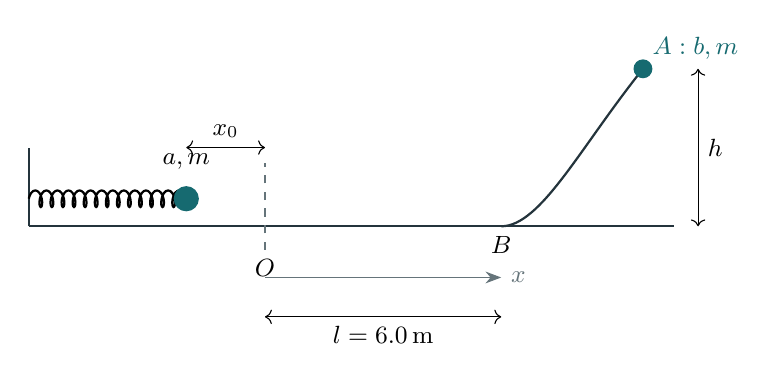
\begin{tikzpicture}[font=\small,spring/.style={decorate,decoration={coil,aspect=.45,segment length=4pt,amplitude=3pt},thick}]
\draw[object](-1,0)--(7.2,0);\draw[object](-1,0)--(-1,1);
\draw[spring](-1,.35)--(1,.35);\fill[accent](1,.35)circle(.16);\node[above]at(1,.6){$a,m$};
\draw[guide](2,-.3)--(2,.8);\node[below]at(2,-.3){$O$};
\draw[object](5,0)..controls(5.5,0)and(6,1)..(6.8,2);
\fill[accent](6.8,2)circle(.12)node[above right]{$A:b,m$};\node[below]at(5,0){$B$};
\draw[<->](1,1)--(2,1)node[midway,above]{$x_0$};
\draw[<->](2,-1.15)--(5,-1.15)node[midway,below]{$l=6.0\,\mathrm m$};
\draw[axis](2,-.65)--(5,-.65)node[right]{$x$};
\draw[<->](7.5,0)--(7.5,2)node[midway,right]{$h$};
\end{tikzpicture}\figcaption{图 7.1}\end{minipage}\end{center}

\Needspace{5\baselineskip}

\pdfbookmark[3]{题型定位}{q1-h0}

\subsection*{题型定位}

匀速来球与简谐振子相遇后粘合。先求第一次交点和两条轨迹的斜率，再由动量求粘合速度，以碰撞位置与速度作为新振动初值。

\Needspace{5\baselineskip}

\pdfbookmark[3]{知识点}{q1-h1}

\subsection*{知识点}

来球在曲面上由重力势能转化出动能，进入水平面后匀速运动。短暂粘合满足水平动量守恒，弹簧势能在碰撞前后相同。质量增加使频率改为 $\omega/\sqrt{1+\eta}$，碰后位移和速度共同确定振幅与相位。


\Needspace{5\baselineskip}

\pdfbookmark[3]{物理图像}{q1-h2}

\subsection*{物理图像}

图7.1中来球从右侧 $B$ 向左运动。解图7.1A的交点给出同一时刻的相同位置，两条切线斜率分别给出碰前速度。解图7.1B的粘合初始相点位于第二象限，其余弦相位由 $v/\omega^{\prime}=-A\sin\phi$ 取第三象限。


\Needspace{5\baselineskip}

\pdfbookmark[3]{解题入口}{q1-h3}

\subsection*{解题入口}

释放时刻取 $t=0$，来球到 $B$ 后另记 $s=t-t_{AB}$。先用振幅范围排除早期相遇，再在 $(3,3.5)$ 内求根。将有向速度 $v_a$、$-v_B$ 代入动量式，最后令碰后时间 $\tau=t-t_c$。

\Needspace{5\baselineskip}

\pdfbookmark[3]{标准解法}{q1-h4}

\subsection*{标准解法}

\begin{center}\begin{minipage}{\linewidth}\centering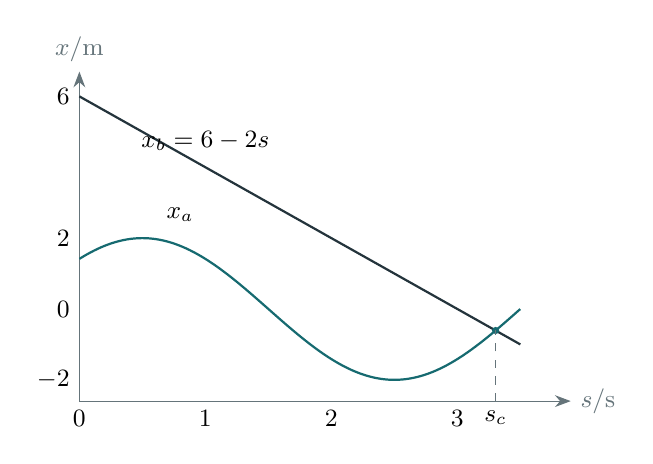
\begin{tikzpicture}[font=\small,x=1.6cm,y=.45cm]
\draw[axis](0,-2.6)--(3.9,-2.6)node[right]{$s/\mathrm s$};
\draw[axis](0,-2.6)--(0,6.7)node[above]{$x/\mathrm m$};
\draw[traj,domain=0:3.5,samples=121]plot(\x,{2*cos(90*\x+315)});
\draw[object](0,6)--(3.5,-1);
\fill[accent](3.303613612,-.607227224)circle(1.3pt);
\draw[guide](3.303613612,-2.6)--(3.303613612,-.607227224);
\node[below]at(3.303613612,-2.6){$s_c$};
\foreach \x in {0,1,2,3}{\node[below]at(\x,-2.6){$\x$};}
\foreach \y in {-2,0,2,6}{\node[left]at(0,\y){$\y$};}
\node[above]at(1,4.2){$x_b=6-2s$};\node[above]at(.8,2.2){$x_a$};
\end{tikzpicture}\figcaption{解图 7.1A}\end{minipage}\end{center}
以平衡点 $O$ 为原点，向右为正；释放时刻记为 $t=0$，碰后另用 $\tau$ 计时。曲面上质点到 $B$ 时由机械能守恒有
\[v_B=\sqrt{2gh}=2.00\,\mathrm{m/s}.\]
它在 $B$ 后向左匀速运动。令 $s=t-t_{AB}\ge0$，两质点的坐标分别为
\[x_b(s)=6-2s,\qquad x_a(s)=-2\cos\left[\frac\pi2(1.5+s)\right]
=2\cos\left(\frac\pi2s+\frac{7\pi}4\right).\]
解图7.1A中直线与正弦曲线的第一次交点才是实际碰撞。方程为
\[6-2s=2\cos\left(\frac\pi2s+\frac{7\pi}4\right).\]
按相同时间步长列表，可先夹住交点：
\begin{center}\begin{tabular}{c|rrrrrrrr}
$s/\mathrm s$&0&0.5&1&1.5&2&2.5&3&3.5\\\hline
$x_b/\mathrm m$&6&5&4&3&2&1&0&$-1$\\
$x_a/\mathrm m$&1.414&2&1.414&0&$-1.414$&$-2$&$-1.414$&0
\end{tabular}\end{center}
$s<2$ 时来球尚在振子右侧；$2\le s\le3$ 时来球非负而振子非正。第一次相遇在 $(3,3.5)$。这段内 $x_b-x_a$ 严格递减，故根唯一。用二分或牛顿迭代求出 $s_c$，再计算
\[t_c=1.5+s_c,\quad x_c=6-2s_c,\quad
v_a=\pi\sin\left[\frac\pi2(1.5+s_c)\right].\]
碰撞期间弹簧冲量可忽略，水平方向动量守恒：
\[2m v_c=m v_a-m v_B,\qquad v_c=\frac{v_a-v_B}{2}.\]
质量变为 $2m$ 后圆频率为 $\omega'=\omega/\sqrt2=\pi/(2\sqrt2)$。因此取碰撞为 $\tau=0$，最直接的表达式为
\[\boxed{x(\tau)=x_c\cos(\omega'\tau)+\frac{v_c}{\omega'}\sin(\omega'\tau).}\]
它在零时刻同时满足 $x(0)=x_c$、$\dot x(0)=v_c$。若改写为 $A\cos(\omega'\tau+\phi)$，则
\[A=\sqrt{x_c^2+(v_c/\omega')^2},\qquad
\phi=\operatorname{atan2}(-v_c/\omega',x_c)\pmod{2\pi}.\]
\begin{center}\begin{minipage}{\linewidth}\centering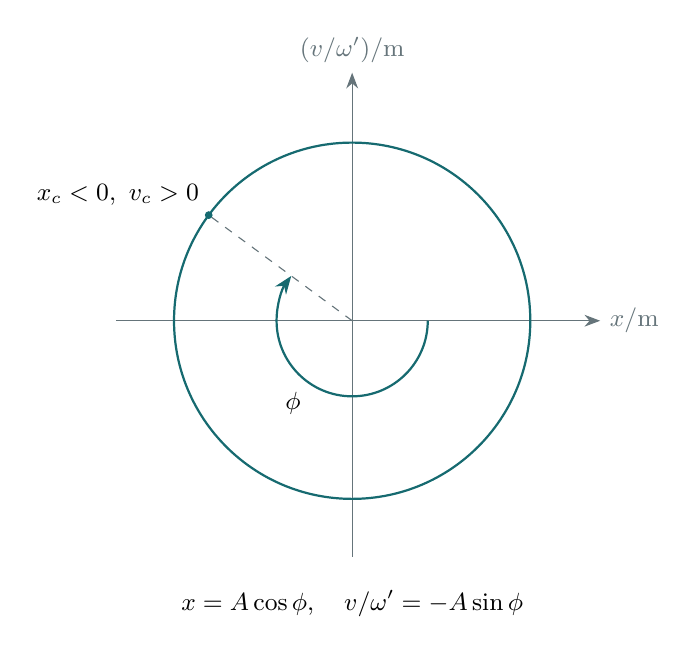
\begin{tikzpicture}[font=\small,x=3cm,y=3cm]
\draw[axis](-1,0)--(1.05,0)node[right]{$x/\mathrm m$};
\draw[axis](0,-1)--(0,1.05)node[above]{$(v/\omega')/\mathrm m$};
\draw[traj](0,0)circle(.754094661);
\fill[accent](-.607227224,.447139638)circle(1.4pt);
\draw[guide](0,0)--(-.607227224,.447139638);
\node[above left]at(-.607227224,.447139638){$x_c<0,\ v_c>0$};
\draw[motion](.32,0)arc(0:-216.3666:.32);
\node at(-.25,-.35){$\phi$};
\node[below]at(0,-1.1){$x=A\cos\phi,\quad v/\omega'=-A\sin\phi$};
\end{tikzpicture}\figcaption{解图 7.1B}\end{minipage}\end{center}
解图7.1B中的初始相点位于 $x<0,v>0$ 区域，满足 $\cos\phi<0,\sin\phi<0$，因此余弦相位在第三象限。下面用交点的未舍入数值计算振幅与相位。
\[\begin{aligned}s_c&=3.303614\,\mathrm s,&t_c&=4.803614\,\mathrm s,\\x_c&=-0.607227\,\mathrm m,&v_a&=2.993295\,\mathrm{m/s},\\v_c&=0.496647\,\mathrm{m/s},&A&=0.754095\,\mathrm m,\\\phi&=3.776309\,\mathrm{rad}& &=216.3666^\circ.\end{aligned}\]
碰撞损失的机械能为 $m(v_a+v_B)^2/4$；它只发生在粘合过程，碰后振动本身守恒机械能。
\subsubsection*{释放、到达曲面底部和碰撞三个时刻}
图7.1以平衡点$O$为零点，压缩量$x_0$是正的长度，
振子的初始坐标却为$-x_0$。
先由释放位置和速度确定碰前振动的两个积分常数，得
\[
x_a(t)=x_0\cos(\omega t+\phi_0),\qquad
x_a(0)=-x_0,\quad\dot x_a(0)=0,
\]
\[
\cos\phi_0=-1,\quad\sin\phi_0=0,
\quad\phi_0=\pi\pmod{2\pi},\qquad
x_a(t)=-2\cos(\pi t/2).
\]
另一质点沿光滑曲面下滑时，支持力不做功，
$mgh=mv_B^2/2$给$v_B=2\,\mathrm{m/s}$。
下滑高度决定到达 $B$ 时的速率，曲面的形状还影响滑行历时。本题直接给出这段历时为 $t_{AB}=1.5\,\mathrm s$。
到达$B$后才作向左匀速运动，因此其位置和速度初值应在$t_{AB}=1.5\,\mathrm s$处接续。
令$s=t-t_{AB}$，代入振子方程的相位应逐项为
\[
\omega(t_{AB}+s)+\pi
=\frac\pi2s+\frac34\pi+\pi
=\frac\pi2s+\frac74\pi.
\]
这样在 $s=0$ 时，振子已经运动 $t_{AB}$，位置和速度从释放状态接续而来。

\subsubsection*{第一次相遇的筛选和数值迭代}
解图7.1A的两条曲线按同一时间、位置刻度绘制。
设$F(s)=x_b(s)-x_a(s)$。
对$0\leq s<2$，$x_b>2\,\mathrm m$而$x_a\leq2\,\mathrm m$，没有相遇；
$s=2$时$x_b=2$、$x_a=-\sqrt2$，也不相等。
在$2\leq s\leq3$上，$x_b\geq0$而$x_a<0$，仍不相遇。
接着计算
\[
F(3)=\sqrt2>0,\qquad F(3.5)=-1<0.
\]
该区间内$\pi s/2+7\pi/4$按$2\pi$约去后位于$[5\pi/4,3\pi/2]$，
所以其正弦为负，
\[
F'(s)=-2+\pi\sin\left(\frac\pi2s+\frac{7\pi}4\right)<-2<0.
\]
因而这里有且仅有一个根，并且就是实际发生的第一次碰撞。
二分法保持$F$异号的两端；若用牛顿法，则迭代式为
\[
s_{n+1}=s_n-
\frac{6-2s_n-2\cos(\pi s_n/2+7\pi/4)}
{-2+\pi\sin(\pi s_n/2+7\pi/4)}.
\]
以$s_0=3.3$起算，可收敛到$s_c=3.303613612\cdots$。
在求根和随后计算中保留这些有效位，最后才按所需精度取值。
将根代回两条轨迹，分别得到同一$x_c$，
而碰前速度须分别求斜率：
\[
\dot x_b=-2,\qquad
\dot x_a=-\pi\sin\left(\frac\pi2s+\frac{7\pi}4\right).
\]
这与$\dot x_a=\pi\sin[\pi(1.5+s)/2]$完全相同，
振子的速度为正，来球速度为负，二者迎面碰撞。动量式中的两个有向速度分别是 $v_a$ 和 $-v_B$。

\subsubsection*{碰后初值、振幅及相位的完整恢复}
碰撞历时远小于振动周期，弹簧在这段时间内可以取碰撞位置处的伸长量。弹簧的冲量可略，两物体以碰前速度的质量加权平均值一同运动。
动量守恒计算的中间数值为
\[
v_c=\frac{2.993294535-2}{2}
=0.496647267\cdots\,\mathrm{m/s},
\qquad \omega'=\frac{\pi}{2\sqrt2}=1.110720735\cdots\,\mathrm{s}^{-1}.
\]
将碰后时间记为$\tau$，线性组合中两项系数由初值分别确定：
\[
x=C_1\cos\omega'\tau+C_2\sin\omega'\tau,
\quad C_1=x_c,
\quad \dot x(0)=\omega'C_2=v_c,
\quad C_2=v_c/\omega'.
\]
因此可直接给出带数值的振动式
\[
x(\tau)=
(-0.607227224\cdots)\cos(1.110720735\cdots\tau)
+(0.447139638\cdots)\sin(1.110720735\cdots\tau)
\quad\mathrm m.
\]
展开幅相式$A\cos(\omega'\tau+\phi)$并逐项比较，
\[
A\cos\phi=x_c<0,\qquad
-A\sin\phi=v_c/\omega'>0.
\]
所以$\cos\phi<0$且$\sin\phi<0$，$\phi$在第三象限，
而解图7.1B中的相点$(x,v/\omega')$在第二象限；
由 $v/\omega^{\prime}=-A\sin\phi$，相点从正横轴量起的极角为 $-\phi$。
\[
\phi=\pi+\arctan\frac{v_c}{\omega'|x_c|}
=3.776308779\cdots\,\mathrm{rad},
\quad A=0.754094661\cdots\,\mathrm m.
\]
据此也可写成$x=A\cos(1.110720735\cdots\tau+3.776308779\cdots)$。
$\cos\phi$ 的符号由左侧位置给出，$\sin\phi$ 的符号由向右的初速度给出。这两个符号将正切相同而相差 $\pi$ 的候选相位区分开。

\subsubsection*{碰撞损失与后续振动能量}
碰撞前后弹簧势能相同，故失能只由两质点动能差计算：
\[
\begin{aligned}
Q&=\frac m2(v_a^2+v_B^2)
-\frac12(2m)\left(\frac{v_a-v_B}{2}\right)^2\\
&=\frac m4(v_a^2+2v_av_B+v_B^2)
=\frac m4(v_a+v_B)^2>0.
\end{aligned}
\]
碰后则是质量$2m$的单一振子，
\[
E_f=mv_c^2+\frac12kx_c^2
=\frac12k\left(x_c^2+\frac{v_c^2}{\omega'^2}\right)
=\frac12kA^2.
\]
第一式用$2m$计平动能，第二式代入 $k=2m\omega^{\prime 2}$ 将速度项改写为位移平方。
碰撞中的动能损失与碰后振动的机械能守恒属于不同时间段。


\Needspace{5\baselineskip}

\pdfbookmark[3]{关键洞察}{q1-h5}

\subsection*{关键洞察}

碰撞位置连续，粘合速度由两物体的动量确定，新的惯性质量决定频率。用 $x_c\cos\omega_c\tau+(v_c/\omega_c)\sin\omega_c\tau$ 可让位移与速度分别进入两个系数，再由两系数恢复振幅与相位。


\Needspace{5\baselineskip}

\pdfbookmark[3]{易错点}{q1-h6}

\subsection*{易错点}

\begin{itemize}
\item $s=0$ 时振子已运动 $t_{AB}$，其相位包含这段时间。
\item 来球速度向左，在向右为正的动量式中取 $-v_B$。
\item 粘合体的质量为两质量之和，振幅式中的频率也取碰后频率。
\item 余弦相位满足 $A\cos\phi=x_c$、$-A\omega_c\sin\phi=v_c$。
\end{itemize}


\Needspace{5\baselineskip}

\pdfbookmark[3]{课堂讲解建议}{q1-h7}

\subsection*{课堂讲解建议}

让学生在解图7.1A上标出释放、到达 $B$ 和碰撞三个时刻。来球在振子振幅范围以外时先排除相遇，再利用两条曲线的单调性找到第一次交点。

在交点分别作两条切线，问两物体各向哪边运动。将相应有向速度写入动量式，再从质量变化说明 $\omega_c$ 的取值。在解图7.1B上标出 $x_c$ 和 $v_c/\omega_c$，由余弦和正弦的符号选相位。

比较变图7.1V1中不同来球质量对应的振幅。图中每一点都使用相同碰前轨迹，变化的是粘合速度与新频率，因而两者同时进入振幅计算。


\Needspace{5\baselineskip}

\pdfbookmark[3]{变式训练}{q1-h8}

\subsection*{变式训练}

\begin{enumerate}
\item 令来球质量为 $\eta m$，初始运动条件保持题给值。曲面与水平运动均由加速度决定，因此相遇位置与时刻仍为 $x_c,t_c$。向右取正，
\[
mv_a-\eta mv_B=(1+\eta)mv_c,\qquad
v_c=\frac{v_a-\eta v_B}{1+\eta},\qquad
\omega_c=\frac{\omega}{\sqrt{1+\eta}}.
\]
碰后振幅与相位为
\[
A^2=x_c^2+\frac{(v_a-\eta v_B)^2}{(1+\eta)\omega^2},
\qquad
\phi=\operatorname{atan2}(-v_c/\omega_c,x_c)\pmod{2\pi}.
\]
变图7.1V1给出振幅随来球质量的变化。取 $\eta=2$ 时，$v_c\approx-0.33557\,\mathrm{m/s}$，$\omega_c\approx0.90690\,\mathrm{s}^{-1}$，振幅约为 $0.7111\,\mathrm m$。粘合损失的一般式为 $\eta m(v_a+v_B)^2/[2(1+\eta)]$，可由约化质量直接求得。
\begin{center}\begin{minipage}{.98\linewidth}\centering
\begin{tikzpicture}[scale=.85,transform shape]
\draw[axis](0,0)--(6.9,0)node[right]{$\eta$};
\draw[axis](0,0)--(0,3.5)node[above]{$A/\mathrm m$};
\draw[traj,domain=0:3,samples=100]plot({2*\x},{1.45*sqrt(.607227224^2+(2.993294535-2*\x)^2/((1+\x)*(pi/2)^2))});
\foreach \e in {1,2}{\fill ({2*\e},{1.45*sqrt(.607227224^2+(2.993294535-2*\e)^2/((1+\e)*(pi/2)^2))})circle(1.6pt);\node[below]at({2*\e},0){$\e$};}
\node[left]at(0,1.45){$1$};
\end{tikzpicture}
\figcaption{变图7.1V1\quad 来球质量变化同时影响碰后速度与频率}
\end{minipage}\end{center}
\item 改为等质量完全弹性碰撞。短时间内动量与动能守恒，解得两质点交换速度。振子碰后速度为 $-v_B$，自由球速度为 $v_a$。振子的质量仍为 $m$，所以
\[
x_{\rm osc}=x_c\cos\omega\tau-\frac{v_B}{\omega}\sin\omega\tau,\qquad
A_{\rm el}=\sqrt{x_c^2+(v_B/\omega)^2}.
\]
自由球的位置为 $x_{\rm free}=x_c+v_a\tau$，对应变图7.1V2中的上升直线。它约在 $0.674\,\mathrm s$ 到达振子最大右伸位置 $A_{\rm el}$；振子到此时还在向左运动，首次左端转折约在 $0.717\,\mathrm s$。此前两者间距一直增大，此后自由球已在振动范围右侧，故这一初态下不会再次相撞。
\begin{center}\begin{minipage}{.98\linewidth}\centering
\begin{tikzpicture}[scale=.85,transform shape]
\draw[axis](0,0)--(6.5,0)node[right]{$\omega\tau$};
\draw[axis](0,-2)--(0,3)node[above]{$x/\mathrm m$};
\draw[traj,domain=0:4,samples=90]plot({1.4*\x},{-.607227224*cos(deg(\x))-2/(pi/2)*sin(deg(\x))});
\draw[motion,-,domain=0:1.5,samples=45]plot({1.4*\x},{-.607227224+2.993294535*\x/(pi/2)});
\node[right]at(2.1,2.25){自由球};
\node[right]at(5.45,1.4){弹簧振子};
\draw[guide](0,1.410627)--(5.6,1.410627)node[right]{$A_{\rm el}$};
\end{tikzpicture}
\figcaption{变图7.1V2\quad 弹性碰撞后自由球向右离开，振子先向左运动}
\end{minipage}\end{center}
\item 调节释放条件，使粘合恰在 $O$ 发生。此时 $x_c=0$，由短时动量求得有向初速 $v_c$，粘合体质量所对应的频率为 $\omega_c$。解为
\[
x(\tau)=\frac{v_c}{\omega_c}\sin\omega_c\tau,\qquad A=\frac{|v_c|}{\omega_c}.
\]
变图7.1V3取 $v_c>0$，四分之一周期首次到达右端。若写作余弦形式，$A\cos\phi=0$、$-A\sin\phi>0$，得到 $\phi=3\pi/2$ 模 $2\pi$。
\begin{center}\begin{minipage}{.98\linewidth}\centering
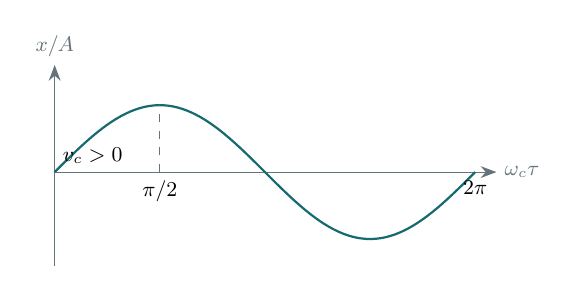
\begin{tikzpicture}[scale=.85,transform shape]
\draw[axis](0,0)--(6.6,0)node[right]{$\omega_c\tau$};
\draw[axis](0,-1.4)--(0,1.6)node[above]{$x/A$};
\draw[traj,domain=0:6.283185,samples=90]plot(\x,{sin(deg(\x))});
\draw[guide](1.570796,0)--(1.570796,1);
\node[below]at(1.570796,0){$\pi/2$};
\node[above right]at(0,0){$v_c>0$};
\node[below]at(6.283185,0){$2\pi$};
\end{tikzpicture}
\figcaption{变图7.1V3\quad 平衡点粘合且初速向右，位移从零开始增加}
\end{minipage}\end{center}
\item 另将两物体放在同一非零位置 $x_c$，均从静止开始粘合。动量式给 $v_c=0$，于是
\[
x(\tau)=x_c\cos\omega_c\tau,\qquad A=|x_c|.
\]
变图7.1V4的初始相点在椭圆的左端，回复力向右。粘合增加惯性，使周期取 $2\pi/\omega_c$，初始势能 $kx_c^2/2$ 决定转折距离。若两物体初始就在 $O$ 且均静止，则保持平衡。
\begin{center}\begin{minipage}{.98\linewidth}\centering
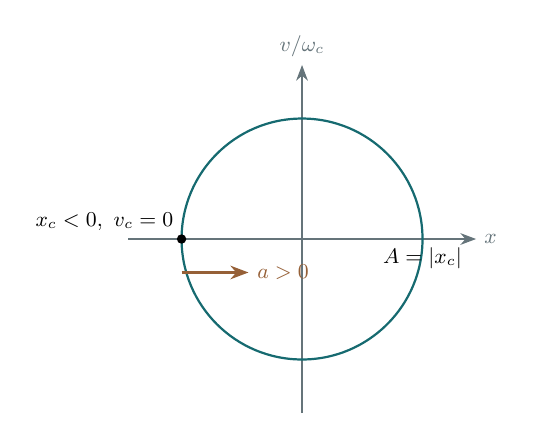
\begin{tikzpicture}[scale=.85,transform shape]
\draw[axis](-2.6,0)--(2.6,0)node[right]{$x$};
\draw[axis](0,-2.6)--(0,2.6)node[above]{$v/\omega_c$};
\draw[traj](0,0)circle(1.8);
\fill(-1.8,0)circle(2pt)node[above left]{$x_c<0,\ v_c=0$};
\draw[force](-1.8,-.5)--(-.8,-.5)node[right]{$a>0$};
\node[below]at(1.8,0){$A=|x_c|$};
\end{tikzpicture}
\figcaption{变图7.1V4\quad 两物体在同一位置静置粘合，初态是转折点}
\end{minipage}\end{center}
\item 用自释放时刻起算的总时间 $t$ 写碰后解。变图7.1V5在同一时间轴标出 $t_{AB}$ 与 $t_c$。由于 $\tau=t-t_c$，
\[
x(t)=x_c\cos[\omega_c(t-t_c)]
+\frac{v_c}{\omega_c}\sin[\omega_c(t-t_c)],\qquad t\geq t_c.
\]
若碰后原写作 $A\cos(\omega_c\tau+\phi_\tau)$，展开相位得 $\phi_t=\phi_\tau-\omega_ct_c$。在 $t=t_c$，两个三角函数的自变量同时归零，位置为 $x_c$，速度为 $v_c$。
\begin{center}\begin{minipage}{.98\linewidth}\centering
\begin{tikzpicture}[scale=.85,transform shape]
\draw[axis](0,0)--(7.7,0)node[right]{$t$};
\fill(1.1,0)circle(1.8pt)node[below]{$0$（释放）};
\fill(3.2,0)circle(1.8pt)node[below]{$t_{AB}$};
\fill(6.0,0)circle(1.8pt)node[below]{$t_c$};
\draw[<->](3.2,.6)--(6,.6)node[midway,above]{$s_c$};
\draw[axis](6,1.65)--(7.7,1.65)node[right]{$\tau$};
\draw[guide](6,0)--(6,1.65)node[above left]{$\tau=0$};
\end{tikzpicture}
\figcaption{变图7.1V5\quad 两个时间原点相隔碰撞时刻，位置曲线按同一初态接续}
\end{minipage}\end{center}
\item 求等质量粘合碰撞的机械能损失。变图7.1V6只比较碰撞前后的动能，弹簧在两侧处于同一伸长。将 $v_c=(v_a-v_B)/2$ 代入，
\[
Q=\frac12m(v_a^2+v_B^2)-m\left(\frac{v_a-v_B}{2}\right)^2
=\frac m4(v_a+v_B)^2.
\]
题给数值对应 $Q/m\approx6.23325\,\mathrm{m^2/s^2}$。碰后剩余的机械能为 $mv_c^2+kx_c^2/2=kA^2/2$，它在粘合后的振动中于弹性势能和平动动能之间转换。
\begin{center}\begin{minipage}{.98\linewidth}\centering
\begin{tikzpicture}[scale=.85,transform shape]
\draw[axis](0,0)--(6.5,0)node[right]{能量};
\fill[accent!18](0,.65)rectangle(6.7,1.2);
\fill[warm!20](0,1.6)rectangle(.255,2.15);
\draw[<->](.255,2.35)--(6.7,2.35)node[midway,above]{$Q$};
\node[left]at(0,.92){碰前动能};
\node[left]at(0,1.87){碰后动能};
\node[below]at(3.4,-.25){弹簧势能在碰撞前后相同};
\end{tikzpicture}
\figcaption{变图7.1V6\quad 由两物体动能之差计算粘合耗散}
\end{minipage}\end{center}
\end{enumerate}


\Needspace{18\baselineskip}

\pdfbookmark[2]{第 2 题 密度线性分层液体中的浮力振动}{q2}

\section*{第 2 题\quad 密度线性分层液体中的浮力振动}

\tagline{M-07-02}

如图,某液体的密度随深度线性地增加,液体表面的密度为\(\rho_{0}\),深度为\(D\)处的密度为\(2\rho_{0}\),一密度为\(2\rho_{0}\)的小球在深度为\(\frac{D}{2}\)处从静止释放.忽略液体的阻力.试求小球的振动表达式.

小球尺度远小于密度变化长度；密度规律在运动所达深度内成立，忽略液体附加质量。

\begin{center}\begin{minipage}{\linewidth}\centering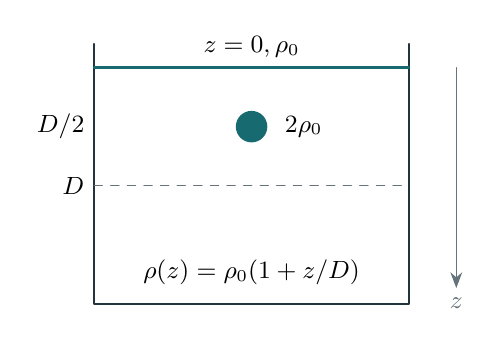
\begin{tikzpicture}[line cap=round,line join=round,spring/.style={decorate,decoration={coil,aspect=.45,segment length=4pt,amplitude=3pt},thick}]\draw[object] (0,3)--(0,-.3)--(4,-.3)--(4,3);\draw[traj] (0,2.7)--(4,2.7);\node[above] at (2,2.7) {$z=0,\rho_0$};\draw[axis] (4.6,2.7)--(4.6,-.1) node[below] {$z$};\draw[guide](0,1.2)--(4,1.2);\node[left]at(0,1.2){$D$};\fill[accent] (2,1.95) circle (.2);\node[right] at (2.3,1.95) {$2\rho_0$};\node[left] at (0,1.95) {$D/2$};\node at (2,.1) {$\rho(z)=\rho_0(1+z/D)$};\end{tikzpicture}\figcaption{图 7.2}\end{minipage}\end{center}

\Needspace{5\baselineskip}

\pdfbookmark[3]{题型定位}{q2-h0}

\subsection*{题型定位}

液体密度随深度线性增加，使完全浸没的小球受到线性回复力。先找浮重平衡深度，再将深度平移为平衡位移。

\Needspace{5\baselineskip}

\pdfbookmark[3]{知识点}{q2-h1}

\subsection*{知识点}

小球质量为 $\rho_sV$，浮力为 $\rho(z)Vg$。密度的正梯度提供回复系数，除以惯性质量得到频率。线性模型内频率由梯度与球密度决定，释放位置和初速度决定振幅与相位。


\Needspace{5\baselineskip}

\pdfbookmark[3]{物理图像}{q2-h2}

\subsection*{物理图像}

解图7.2A中浅端 $D/2$ 的重力大于浮力，球从静止向下加速。经过 $D$ 时两力相等而速度最大，随后浮力占优，球仍向下运动至 $3D/2$ 才停止。解图7.2B的曲线高度是深度，其斜率是向下速度。


\Needspace{5\baselineskip}

\pdfbookmark[3]{解题入口}{q2-h3}

\subsection*{解题入口}

由两处密度值写出 $\rho(z)=\rho_0(1+z/D)$，用 $m=2\rho_0V$ 列向下的合力。令合力为零求得 $z_e=D$，再设 $x=z-D$，将释放条件改为 $x(0)=-D/2,\dot x(0)=0$。

\Needspace{5\baselineskip}

\pdfbookmark[3]{标准解法}{q2-h4}

\subsection*{标准解法}

\begin{center}\begin{minipage}{\linewidth}\centering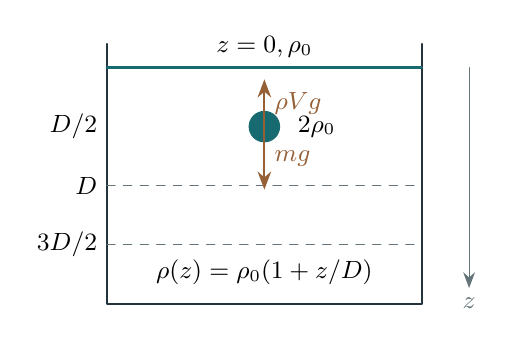
\begin{tikzpicture}[line cap=round,line join=round,spring/.style={decorate,decoration={coil,aspect=.45,segment length=4pt,amplitude=3pt},thick}]\draw[object] (0,3)--(0,-.3)--(4,-.3)--(4,3);\draw[traj] (0,2.7)--(4,2.7);\node[above] at (2,2.7) {$z=0,\rho_0$};\draw[axis] (4.6,2.7)--(4.6,-.1) node[below] {$z$};\draw[guide] (0,1.2)--(4,1.2);\node[left]at(0,1.2){$D$};\fill[accent] (2,1.95) circle (.2);\node[right] at (2.3,1.95) {$2\rho_0$};\node[left] at (0,1.95) {$D/2$};\node at (2,.1) {$\rho(z)=\rho_0(1+z/D)$};\draw[force](2,1.95)--(2,1.15)node[midway,right]{$mg$};\draw[force](2,1.95)--(2,2.55)node[midway,right]{$\rho Vg$};\draw[guide] (0,.45)--(4,.45);\node[left]at(0,.45){$3D/2$};\end{tikzpicture}\figcaption{解图 7.2A}\end{minipage}\end{center}
解图7.2A以液面为零深度，$z$ 向下为正。线性密度规律由两个给定值确定：
\[\rho(z)=\rho_0+\frac{\rho_0}{D}z=\rho_0(1+z/D).\]
设球体积为 $V$，质量为 $m=2\rho_0V$。重力向下，浮力向上，故
\[m\ddot z=mg-\rho(z)Vg
=\rho_0Vg(1-z/D),\qquad
\ddot z+\frac g{2D}(z-D)=0.\]
浮力所用的密度是小球所在深度的液体密度。若球从$z$向下再移$\Delta z$，重力不变，浮力增加$\rho_0Vg\Delta z/D$，因而合力变化为
\[\Delta F_z=-\frac{\rho_0Vg}{D}\Delta z.\]
这个负斜率给回复系数$K=\rho_0Vg/D$；除以球自身质量$2\rho_0V$才得到$\omega^2$。给定密度在所用液层中为线性函数，所以回复合力在整个运动范围内都与 $x$ 成正比。

平衡深度为 $z_e=D$。令 $x=z-D$，才有齐次的简谐方程
\[\ddot x+\omega^2x=0,\qquad\omega=\sqrt{g/(2D)}.\]
从深度 $D/2$ 静止释放，初值是 $x(0)=-D/2$、$\dot x(0)=0$，因此
\[x(t)=-\frac D2\cos(\omega t),\qquad
\boxed{z(t)=D-\frac D2\cos\left(\sqrt{\frac g{2D}}t\right).}\]
解图7.2A的初始位置在平衡点上方，故$z(0)<D$时向下合力为正，初始加速度应向下。由解得
\[\dot z=\frac D2\omega\sin\omega t,
\qquad \dot z(T/4)=\frac D2\omega=\sqrt{gD/8}.\]
四分之一周期到达平衡点时速率最大，半周期到图中的深端并瞬时停下。余弦项在初始时取负值，表示从上方浅端释放。

解图中的两个转折深度为 $D/2$ 与 $3D/2$，相应平衡位移为 $-D/2$ 与 $D/2$。液面深度由平衡位移加上 $D$ 得到。本题按小球自身质量计惯性，线性密度规律覆盖它经过的整个液层。
也可定义相对于平衡的有效势能 $U=\rho_0Vg x^2/(2D)$；由 $m\dot x^2/2+U$ 守恒得到同一频率。
\subsubsection*{合力、平衡位移和释放初值的逐步代入}
解图7.2A的$z$从液面向下量，$x=z-D$从平衡深度量。
在同一初态，两种坐标分别是$z_0=D/2$和$x_0=-D/2$。
先代质量和密度，再约去共同的$\rho_0V$，
\[
2\rho_0V\ddot z=2\rho_0Vg-
\rho_0\left(1+\frac zD\right)Vg,
\]
\[
\ddot z=\frac g2-\frac g{2D}z
=-\frac g{2D}(z-D).
\]
因此在液面下深度 $D$ 处浮力与重力相等。
令$x=A\cos(\omega t+\phi)$，
释放条件给
\[
A\cos\phi=-D/2,\qquad -A\omega\sin\phi=0,
\quad A=D/2,\quad\phi=\pi.
\]
这恢复$x=-(D/2)\cos\omega t$，加回$D$才是题目所问的液面下深度。
周期为$T=2\pi\sqrt{2D/g}$；频率量纲为$1/\mathrm s$，与球体积无关。

\subsubsection*{浅端、平衡点与深端的浮力和速率}
初态$z=D/2$处液体密度为$3\rho_0/2$，
浮力与重力之比是$3/4$，故初始向下加速度为$g/4$。
在$z=D$，两力相等、加速度为零，但速率最大；
在$z=3D/2$，浮力与重力之比为$5/4$，加速度为向上的$g/4$，
速度则在转折瞬间为零。
在解图7.2B中，曲线从浅端以零斜率出发，深度随向下加速而增加。过平衡深度时斜率绝对值最大，到深端时斜率降为零，随后开始上浮。
\begin{center}\begin{minipage}{\linewidth}\centering
\begin{tikzpicture}[x=.95cm,y=1.65cm,font=\small]
\draw[axis](0,.25)--(6.7,.25)node[right]{$\omega t$};
\draw[axis](0,.25)--(0,1.85)node[above]{$z/D$};
\draw[traj,domain=0:6.283185307,samples=101]plot(\x,{1-.5*cos(\x*180/pi)});
\draw[guide](0,1)--(6.283185307,1);
\foreach \x/\lab in {1.570796327/{\pi/2},3.141592654/{\pi},4.712388980/{3\pi/2},6.283185307/{2\pi}}
 {\draw(\x,.25)--(\x,.2);\node[below]at(\x,.2){$\lab$};}
\foreach \y/\lab in {.5/{1/2},1/{1},1.5/{3/2}}{\node[left]at(0,\y){$\lab$};}
\fill(0,.5)circle(1.1pt);\fill(3.141592654,1.5)circle(1.1pt);
\node[above]at(3.141592654,1.5){最深，$v=0$};
\end{tikzpicture}
\figcaption{解图7.2B\quad 深度先增后减，过平衡位置时曲线的斜率绝对值最大。}
\end{minipage}\end{center}
回复合力$F_z=-Kx$对应
\[
K=\frac{\rho_0Vg}{D},\qquad
U(x)=\int_0^x K\xi\dd\xi=\frac12Kx^2.
\]
从静止释放，能量常数为
\[
E=\frac12K(D/2)^2=\frac{\rho_0VgD}{8}
=\frac{mgD}{16}.
\]
到平衡点时$U=0$，$mv_{\max}^2/2=mgD/16$给
$v_{\max}=\sqrt{gD/8}$，与对振动式求导相同。
另一转折点满足同一$U$而位移反号，故$x=D/2$、$z=3D/2$。

\subsubsection*{液面、底部和密度模型的范围}
小球的中心运动范围为$D/2\leq z\leq3D/2$。
若球的半径为 $r$，浅端的球顶深度为 $D/2-r$，深端的球底深度为 $3D/2+r$。前者为正、后者小于容器深度，给出完全浸没且无底面接触的范围。题设用无阻力、无附加质量的小球模型，因而回复系数除以球自身质量得到频率。


\Needspace{5\baselineskip}

\pdfbookmark[3]{关键洞察}{q2-h5}

\subsection*{关键洞察}

浮力梯度给出 $K=\rho_0Vg/D$，球的惯性质量为 $2\rho_0V$，因此 $\omega^2=g/(2D)$。绝对深度和回复力中的位移相差 $D$，同一个运动可分别用 $z(t)$ 与 $x(t)$ 表示。


\Needspace{5\baselineskip}

\pdfbookmark[3]{易错点}{q2-h6}

\subsection*{易错点}

\begin{itemize}
\item 球密度 $\rho_s=2\rho_0$ 为常量，液体密度 $\rho(z)$ 随深度改变。
\item 回复合力写成 $-Kx$ 时，$x=z-D$ 从平衡点量起。
\item 球的运动范围由两个转折深度连同半径确定，整个球体所占区域都处于题设液层内。
\end{itemize}


\Needspace{5\baselineskip}

\pdfbookmark[3]{课堂讲解建议}{q2-h7}

\subsection*{课堂讲解建议}

先在解图7.2A的三个标记深度分别比较重力与浮力。要求同时画速度和加速度箭头，说明球经过 $D$ 后受到向上的合力，向下速度仍会持续一段时间。

写出液面坐标中的非齐次方程，再把 $z$ 换成 $D+x$。让学生将两个坐标的初值对应到同一点，随后沿解图7.2B读出四分之一周期和半周期处的深度与斜率。用变图7.2V5比较只改变惯性时周期怎样变化，回复力曲线保持题给梯度。


\Needspace{5\baselineskip}

\pdfbookmark[3]{变式训练}{q2-h8}

\subsection*{变式训练}

\begin{enumerate}
\item 球密度改为 $c\rho_0$。变图7.2V1中平衡由球密度的水平线与液体密度线相交确定，故
\[
z_e=(c-1)D,\qquad
c\rho_0V\ddot x=-\frac{\rho_0Vg}{D}x,\qquad
\omega_c^2=\frac{g}{cD}.
\]
对所取液面以下的完全浸没平衡，$c>1$，并按小球半径与容器深度选择可达的 $z_e$。球密度提高时，平衡位置加深，惯性增大而浮力梯度相同，周期随 $\sqrt c$ 增大。
\begin{center}\begin{minipage}{.98\linewidth}\centering
\begin{tikzpicture}[scale=.85,transform shape]
\draw[axis](0,0)--(6.3,0)node[right]{$z/D$};
\draw[axis](0,0)--(0,3.2)node[above]{$\rho/\rho_0$};
\draw[traj](0,1)--(4,3)node[right]{液体};
\draw[guide](0,1.5)--(4,1.5)node[right]{$c=1.5$};
\draw[guide](0,2.5)--(4,2.5)node[right]{$c=2.5$};
\fill(1,1.5)circle(1.7pt);\fill(3,2.5)circle(1.7pt);
\node[below]at(1,0){$0.5$};\node[below]at(3,0){$1.5$};
\end{tikzpicture}
\figcaption{变图7.2V1\quad 球密度的水平线与液体密度线的交点给出平衡深度}
\end{minipage}\end{center}
\item 在平衡深度 $D$ 给球向下速度 $u$。初位移为零，初速度为 $u$，积分常数依次确定为
\[
x=C_1\cos\omega t+C_2\sin\omega t,\quad
C_1=0,\quad C_2=\frac u\omega,\quad
z=D+\frac u\omega\sin\omega t.
\]
变图7.2V2取 $u>0$，深端与浅端为 $D+|u|/\omega$ 和 $D-|u|/\omega$。若球半径为 $r$，球体扫过的最浅和最深位置分别为 $D-|u|/\omega-r$ 与 $D+|u|/\omega+r$。前一深度取正，后一深度小于池底深度，整个球始终处于给定的分层液体中。
\begin{center}\begin{minipage}{.98\linewidth}\centering
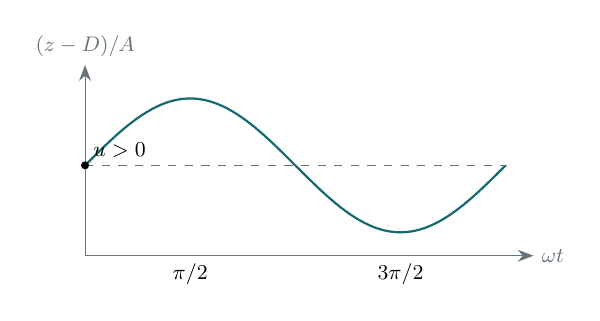
\begin{tikzpicture}[scale=.85,transform shape]
\draw[axis](0,-1.35)--(6.7,-1.35)node[right]{$\omega t$};
\draw[axis](0,-1.35)--(0,1.5)node[above]{$(z-D)/A$};
\draw[traj,domain=0:6.283185,samples=90]plot(\x,{sin(deg(\x))});
\draw[guide](0,0)--(6.3,0);
\fill(0,0)circle(1.7pt)node[above right]{$u>0$};
\node[below]at(1.570796,-1.35){$\pi/2$};
\node[below]at(4.712389,-1.35){$3\pi/2$};
\end{tikzpicture}
\figcaption{变图7.2V2\quad 平衡点向下出发，先达到较深的转折位置}
\end{minipage}\end{center}
\item 液体密度为 $\rho_{\rm top}+bz$，球密度为 $\rho_s$。令浮力等于重力，
\[
z_e=\frac{\rho_s-\rho_{\rm top}}b .
\]
将 $z=z_e+x$ 代入合力，常量项相消，得
\[
\rho_sV\ddot x=-bVgx,\qquad \omega^2=\frac{bg}{\rho_s}.
\]
变图7.2V3的回复力是过原点的斜直线。$b>0$ 时斜率为负，围绕可达的完全浸没平衡振动；给定 $x_i,u_i$ 后，$x=x_i\cos\omega t+(u_i/\omega)\sin\omega t$。
\begin{center}\begin{minipage}{.98\linewidth}\centering
\begin{tikzpicture}[scale=.85,transform shape]
\draw[axis](-2.7,0)--(2.7,0)node[right]{$x=z-z_e$};
\draw[axis](0,-1.7)--(0,1.9)node[above]{$F_z$};
\draw[traj](-2,1.3)--(2,-1.3)node[right]{$-bVgx$};
\draw[guide](-1.6,0)--(-1.6,1.04);
\draw[force](-1.6,-.35)--(-.6,-.35)node[right]{向下回复};
\draw[force](1.6,.35)--(.6,.35)node[left]{向上回复};
\end{tikzpicture}
\figcaption{变图7.2V3\quad 正密度梯度给负的合力斜率}
\end{minipage}\end{center}
\item 令梯度 $b<0$，并选择参数使存在完全浸没的平衡。球在 $x>0$ 处所排液体更轻，合力沿向下正方向。方程与解为
\[
\ddot x=\Omega^2x,\qquad
\Omega=\sqrt{\frac{|b|g}{\rho_s}},\qquad
x=x_i\cosh\Omega t+\frac{u_i}{\Omega}\sinh\Omega t.
\]
变图7.2V4取 $x_i>0,u_i=0$，曲线从零斜率开始，向下位移加速增长。等价的指数解含 $e^{\Omega t}$ 与 $e^{-\Omega t}$ 两项，初态决定系数。这里假定给定分层在讨论时段内维持。
\begin{center}\begin{minipage}{.98\linewidth}\centering
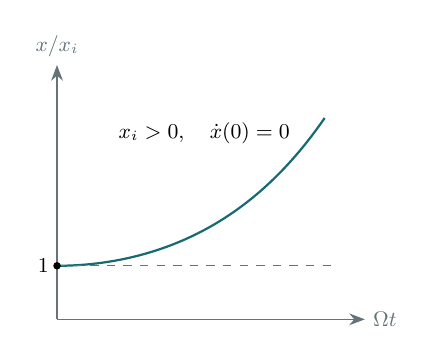
\begin{tikzpicture}[scale=.85,transform shape]
\draw[axis](0,0)--(4.6,0)node[right]{$\Omega t$};
\draw[axis](0,0)--(0,3.8)node[above]{$x/x_i$};
\draw[traj,domain=0:2,samples=60]plot({2*\x},{.8*(exp(\x)+exp(-\x))/2});
\draw[guide](0,.8)--(4.2,.8);
\fill(0,.8)circle(1.6pt)node[left]{$1$};
\node[above]at(2.2,2.5){$x_i>0,\quad\dot x(0)=0$};
\end{tikzpicture}
\figcaption{变图7.2V4\quad 负密度梯度使静止偏离状态继续远离平衡点}
\end{minipage}\end{center}
\item 取恒定的流体附加质量 $m_a$。静止时浮重平衡仍为 $z_e=D$，运动时惯性取 $m+m_a$。因此
\[
\omega_a^2=\frac{\rho_0Vg}{D(m+m_a)}
=\frac{\omega^2}{1+m_a/m},\qquad
T_a=T\sqrt{1+\frac{m_a}{m}} .
\]
变图7.2V5用 $m_a/m$ 为横坐标。附加质量等于球质量时，频率变为 $\omega/\sqrt2$，周期变为 $\sqrt2T$。该变式将 $m_a$ 在运动液层及频率范围内视为常量。
\begin{center}\begin{minipage}{.98\linewidth}\centering
\begin{tikzpicture}[scale=.85,transform shape]
\draw[axis](0,0)--(6.3,0)node[right]{$m_a/m$};
\draw[axis](0,0)--(0,3.3)node[above]{$\omega_a/\omega$};
\draw[traj,domain=0:5.7,samples=80]plot(\x,{2.8/sqrt(1+\x)});
\fill(0,2.8)circle(1.6pt)node[left]{$1$};
\fill(1,1.979899)circle(1.6pt)node[above right]{$(1,1/\sqrt2)$};
\end{tikzpicture}
\figcaption{变图7.2V5\quad 恒定附加质量增加惯性，使频率降低}
\end{minipage}\end{center}
\item 从液面下深度 $z_i$ 以向下初速 $u$ 开始。将初始深度转为 $x_i=z_i-D$，得到
\[
z=D+(z_i-D)\cos\omega t+\frac u\omega\sin\omega t,\qquad
A=\sqrt{(z_i-D)^2+\frac{u^2}{\omega^2}} .
\]
变图7.2V6取 $x_i=-D/2,u=\omega D/4$，相圆满足 $(x/D)^2+[v/(\omega D)]^2=5/16$，因此 $A=\sqrt5D/4$。深度范围为 $D-A$ 至 $D+A$，计入球半径后得到整个球体扫过的液层。初相位由 $\cos\phi=x_i/A$、$\sin\phi=-u/(\omega A)$ 确定。
\begin{center}\begin{minipage}{.98\linewidth}\centering
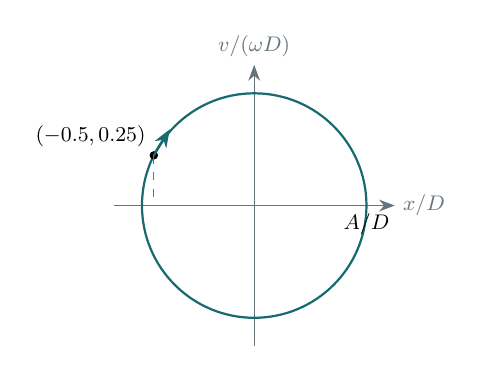
\begin{tikzpicture}[scale=.85,transform shape]
\draw[axis](-2.1,0)--(2.1,0)node[right]{$x/D$};
\draw[axis](0,-2.1)--(0,2.1)node[above]{$v/(\omega D)$};
\draw[traj](0,0)circle(1.677051);
\fill(-1.5,.75)circle(1.8pt)node[above left]{$(-0.5,0.25)$};
\draw[motion](-1.5,.75)--(-1.26,1.14);
\draw[guide](-1.5,.75)--(-1.5,0);
\node[below]at(1.677051,0){$A/D$};
\end{tikzpicture}
\figcaption{变图7.2V6\quad 一般初态在同一相圆上运动，半径决定振幅}
\end{minipage}\end{center}
\end{enumerate}


\clearpage

\pdfbookmark[2]{第 3 题 两滚轮支承木板的微小振动}{q3}

\section*{第 3 题\quad 两滚轮支承木板的微小振动}

\tagline{M-07-03}

如图7.3,两个完全相同的圆柱状滚轮在水平面内平行放置,各绕自身的轴线按图示方向等角速转动,两轴线之间的距离为\(2l\).在两滚轮上平放一块重量为\(G\)的均匀木板,木板与滚轮之间的摩擦系数为\(\mu\).若木板重心偏离两轴中心位置一个微小的距离,试描述木板的运动.

左轮顶面向右、右轮顶面向左。木板视为薄板，微小振动时两接触始终滑动且摩擦方向保持不变。

\begin{center}\begin{minipage}{\linewidth}\centering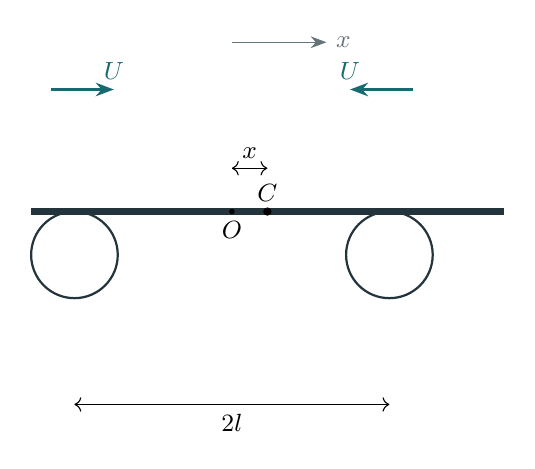
\begin{tikzpicture}[font=\small]
\draw[object,fill=white](0,0)circle(.55);\draw[object,fill=white](4,0)circle(.55);
\draw[object,line width=2.5pt](-.55,.55)--(5.45,.55);
\fill(2.45,.55)circle(1.5pt)node[above]{$C$};\fill(2,.55)circle(1pt)node[below]{$O$};
\draw[motion](-.3,2.1)--(.5,2.1)node[above]{$U$};
\draw[motion](4.3,2.1)--(3.5,2.1)node[above]{$U$};
\draw[axis](2,2.7)--(3.2,2.7)node[right]{$x$};
\draw[<->](0,-1.9)--(4,-1.9)node[midway,below]{$2l$};
\draw[<->](2,1.1)--(2.45,1.1)node[midway,above]{$x$};
\end{tikzpicture}\figcaption{图 7.3}\end{minipage}\end{center}

\Needspace{5\baselineskip}

\pdfbookmark[3]{题型定位}{q3-h0}

\subsection*{题型定位}

支持力随板位置改变，因而两处滑动摩擦的差形成回复合力。由竖直平衡与力矩平衡确定载荷，再列水平运动方程。

\Needspace{5\baselineskip}

\pdfbookmark[3]{知识点}{q3-h1}

\subsection*{知识点}

木板薄且保持水平，摩擦的竖直力臂在该近似下取零。两个支持力之和为重力，力矩给出载荷差；两轮相向的顶面速度维持相反摩擦方向，使载荷差转为线性回复力。


\Needspace{5\baselineskip}

\pdfbookmark[3]{物理图像}{q3-h2}

\subsection*{物理图像}

图7.3的均匀板向右整体移动时，右支点到质心的距离缩短，右支持力增大。解图7.3A中向左的右轮摩擦随之增强，合力向左。解图7.3B给出这支合力随位置变化的负斜率直线。


\Needspace{5\baselineskip}

\pdfbookmark[3]{解题入口}{q3-h3}

\subsection*{解题入口}

取两轮中点为 $O$，从 $N_1+N_2=mg$ 和 $N_1(l+x)=N_2(l-x)$ 求两支持力。将 $F_x=\mu N_1-\mu N_2$ 代入 $m\ddot x=F_x$，用释放条件确定振动相位。

\Needspace{5\baselineskip}

\pdfbookmark[3]{标准解法}{q3-h4}

\subsection*{标准解法}

\begin{center}\begin{minipage}{\linewidth}\centering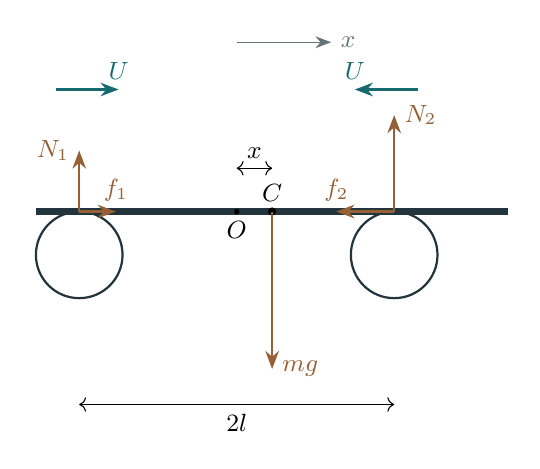
\begin{tikzpicture}[font=\small]
\draw[object,fill=white](0,0)circle(.55);\draw[object,fill=white](4,0)circle(.55);
\draw[object,line width=2.5pt](-.55,.55)--(5.45,.55);
\fill(2.45,.55)circle(1.5pt)node[above]{$C$};\fill(2,.55)circle(1pt)node[below]{$O$};
\draw[motion](-.3,2.1)--(.5,2.1)node[above]{$U$};
\draw[motion](4.3,2.1)--(3.5,2.1)node[above]{$U$};
\draw[axis](2,2.7)--(3.2,2.7)node[right]{$x$};
\draw[<->](0,-1.9)--(4,-1.9)node[midway,below]{$2l$};
\draw[<->](2,1.1)--(2.45,1.1)node[midway,above]{$x$};
\draw[force](0,.55)--(0,1.325)node[left]{$N_1$};
\draw[force](4,.55)--(4,1.775)node[right]{$N_2$};
\draw[force](2.45,.55)--(2.45,-1.45)node[right]{$mg$};
\draw[force](0,.55)--(.465,.55)node[above]{$f_1$};
\draw[force](4,.55)--(3.265,.55)node[above]{$f_2$};
\end{tikzpicture}\figcaption{解图 7.3A}\end{minipage}\end{center}
取两轮中点为 $O$，质心偏移 $x$ 向右为正。左轮顶面向右、右轮顶面向左，故木板受 $f_1=\mu N_1$ 向右、$f_2=\mu N_2$ 向左。薄板竖直方向平衡且不俯仰：
\[N_1+N_2=mg,\qquad N_1(l+x)=N_2(l-x).\]
取木板质心为力矩中心时，左支持点在它左侧$l+x$处，右支持点在它右侧$l-x$处。重力通过质心不贡献力矩，故两支持力的力矩大小相等。将$N_2=mg-N_1$代入，
\[N_1(l+x)=(mg-N_1)(l-x)
\ \Longrightarrow\ 2lN_1=mg(l-x).\]
载荷随质心位置重新分配，中心位置 $x=0$ 对应两轮各承担一半重量。

解得
\[N_1=\frac{mg}{2}(1-x/l),\qquad
N_2=\frac{mg}{2}(1+x/l).\]
解图7.3A显示向右偏移后右轮承重增大；其向左摩擦也增大。于是
\[m\ddot x=f_1-f_2=\mu(N_1-N_2)=-\frac{\mu mg}{l}x.\]
从 $x(0)=a$ 静止释放时
\[\boxed{x(t)=a\cos\left(\sqrt{\frac{\mu g}{l}}t\right),\quad
T=2\pi\sqrt{\frac l{\mu g}}.}\]
解图7.3A中的两个摩擦力始终分别由轮面相对木板的滑动决定。当$x>0$时，$N_2>N_1$，合力向左；当$x<0$时则反向，故合力总与位移反向。将运动方程写成$\ddot x+\Omega^2x=0$，再以初值确定余弦项，所得周期与木板质量无关，是因为载荷产生的摩擦和木板惯性都正比于$m$。驱动装置持续维持两轮转速，两接触持续滑动。装置输入的功率分配给木板动能的变化和接触发热。

取振幅为 $|a|$，两轮都保持正压力时 $|a|<l$。最大板速 $|a|\sqrt{\mu g/l}$ 小于轮顶速率时，两接触的滑动方向在整个周期内均保持图示方向，两支摩擦分别向右和向左。
\subsubsection*{力臂、压力和回复力的全步消元}
图7.3和解图7.3A均以两轮中点为$O$，$C$向右偏$x>0$。
均匀板的几何中心与质心重合，$x$ 同时描述整块木板相对于两轮的水平移动。
左、右支点相对$C$的坐标是$-(l+x)$与$l-x$。
薄板近似把水平摩擦的竖直力臂忽略，支持力矩平衡给
\[
N_1(l+x)=N_2(l-x),\qquad N_2=mg-N_1.
\]
展开右端并把两项$N_1$合并，
\[
N_1[(l+x)+(l-x)]=mg(l-x),\quad
N_1=\frac{mg(l-x)}{2l},
\]
\[
N_2=mg-\frac{mg(l-x)}{2l}
=\frac{mg(l+x)}{2l},\qquad N_1-N_2=-\frac{mg}{l}x.
\]
左轮顶面相对板向右滑，右轮顶面相对板向左滑，
所以取向右为正时，合力为$\mu N_1-\mu N_2$。
两处的相对滑动方向给出水平方向合力的正负号。
\begin{center}\begin{minipage}{\linewidth}\centering
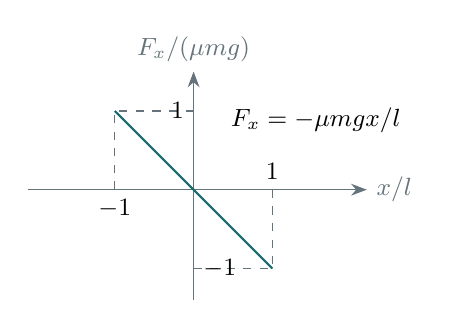
\begin{tikzpicture}[font=\small]
\draw[axis](-2.1,0)--(2.2,0)node[right]{$x/l$};
\draw[axis](0,-1.4)--(0,1.5)node[above]{$F_x/(\mu mg)$};
\draw[traj](-1,1)--(1,-1);
\draw[guide](-1,0)--(-1,1)--(0,1);
\draw[guide](1,0)--(1,-1)--(0,-1);
\node[below]at(-1,0){$-1$};\node[above]at(1,0){$1$};
\node[left]at(0,1){$1$};\node[right]at(0,-1){$-1$};
\node[above right]at(.35,.6){$F_x=-\mu mgx/l$};
\end{tikzpicture}
\figcaption{解图7.3B\quad 固定滑动方向下的回复合力；端点对应左轮或右轮支持力为零。}
\end{minipage}\end{center}
于是$\Omega^2=\mu g/l$，一般初值$x_i,v_i$给
\[
x=x_i\cos\Omega t+\frac{v_i}{\Omega}\sin\Omega t,
\quad A=\sqrt{x_i^2+(v_i/\Omega)^2},\quad v_{\max}=A\Omega.
\]
静止偏移释放只是$v_i=0$的特例。

\subsubsection*{振幅、轮速及有限板长的共同限制}
两接触的相对滑速分别为$U-\dot x$和$-U-\dot x$，
$U>0$是两轮顶面速率。
两接触的滑速分别保持一正一负，给出 $-U<\dot x<U$。用全程最大速率与振幅表示，得到
\[
A\Omega<U,\qquad A<l.
\]
前一条件防止相对滑动反向，后一条件保证两个支持力都严格为正。
若均匀板总长为$L_b$，还需两个滚轮始终落在板的范围内：
\[
L_b/2>l+A.
\]
严格大于时，两个支点在每个转折位置仍位于板内；板的几何范围、两处正压力和相对滑速共同确定这段振动所适用的振幅。

\subsubsection*{驱动功、木板动能和接触发热}
解图7.3A两轮由装置维持$+U,-U$的顶面速度。
木板所受功率为
\[
P_{\rm board}=(f_1-f_2)\dot x
=-\frac{\mu mg}{l}x\dot x=\frac{\dd K_{\rm board}}{\dd t}.
\]
它随位置、速度的乘积变号，摩擦可使板加速也可使板减速。
两轮受到相反的接触反力，维持轮速所需的驱动功率为
\[
P_{\rm drive}=U(f_1+f_2)=\mu mgU.
\]
滑动发热率逐接触相加为
\[
\dot Q=f_1(U-\dot x)+f_2(U+\dot x)
=\mu mgU-(f_1-f_2)\dot x.
\]
故$P_{\rm drive}=\dot Q+\dot K_{\rm board}$，
在所给速度范围内每一接触的发热都非负。
板的方程还可积分成
$K_{\rm board}+\mu mgx^2/(2l)=\text{常量}$，
其中第二项由净回复力对位置积分而定义，它将木板的运动方程写成能量积分的形式。
一完整周期内板动能回到初值，驱动做功$\mu mgUT$全部成为接触热量。


\Needspace{5\baselineskip}

\pdfbookmark[3]{关键洞察}{q3-h5}

\subsection*{关键洞察}

各接触的摩擦与载荷成正比，载荷差随位置线性变化，所以净力为 $-\mu mgx/l$。载荷与惯性质量同时含 $m$，相除后频率与板质量无关。维持轮速的驱动装置则持续供给滑动发热所需能量。


\Needspace{5\baselineskip}

\pdfbookmark[3]{易错点}{q3-h6}

\subsection*{易错点}

\begin{itemize}
\item 摩擦方向由接触点轮面相对板的速度确定，左轮向右、右轮向左。
\item 两支持力相等只对应 $x=0$，偏移时按力矩重新分配。
\item 全过程取 $A<l$、$A\Omega<U$，并用板半长大于 $l+A$ 保证两个支点位于板内。
\end{itemize}


\Needspace{5\baselineskip}

\pdfbookmark[3]{课堂讲解建议}{q3-h7}

\subsection*{课堂讲解建议}

将木板整体右移，先问两个支持力哪一个较大，再在图7.3A上标出两个力臂。由载荷差求净摩擦，沿解图7.3B解释左右两侧的回复方向。

比较变图7.3V1的轮距变化与变图7.3V2的摩擦系数变化，要求学生同时计算频率及最大板速。随后用变图7.3V4解释两摩擦系数不同时平衡点为何移动。最后将电机输入、木板动能变化和接触发热逐项相加，用对应功率式说明整个周期的能量分配。


\Needspace{5\baselineskip}

\pdfbookmark[3]{变式训练}{q3-h8}

\subsection*{变式训练}

\begin{enumerate}
\item 两轮间距从 $2l$ 增为 $4l$，即半轮距变成 $2l$。变图7.3V1中，两力矩的力臂改为 $2l+x$ 与 $2l-x$，消元得
\[
N_1-N_2=-\frac{mgx}{2l},\qquad
\ddot x=-\frac{\mu g}{2l}x,\qquad
\Omega_1=\frac{\Omega}{\sqrt2},\quad T_1=\sqrt2T.
\]
相同板长下，覆盖条件取 $L_b/2>2l+A$。载荷差对位置的变化率减半，因此图中虚线斜率绝对值为实线的一半。水平距离取同一单位 $l$，实线和虚线分别画到 $|x|=l$ 与 $|x|=2l$，端点处一侧支持力降为零；双轮支承的振幅取在端点以内。
\begin{center}\begin{minipage}{.98\linewidth}\centering
\begin{tikzpicture}[scale=.85,transform shape]
\draw[axis](-2.4,0)--(2.6,0)node[right]{$x/l$};
\draw[axis](0,-1.8)--(0,1.85)node[above]{$F_x/(\mu mg)$};
\draw[traj](-1,1)--(1,-1)node[below left]{$2l$轮距};
\draw[object,dashed](-2,1)--(2,-1)node[right]{$4l$轮距};
\foreach \pos in {-2,-1,1,2} {\draw[muted] (\pos,-.08)--(\pos,.08);\node[below] at (\pos,-.08){$\pos$};}
\end{tikzpicture}
\figcaption{变图7.3V1\quad 轮距加倍，净回复力直线的斜率绝对值减半}
\end{minipage}\end{center}
\item 两处动摩擦系数均改为 $4\mu$。支持力仍由原几何分配，净力整体变为四倍，
\[
\ddot x=-\frac{4\mu g}{l}x,\qquad
\Omega_2=2\Omega,\qquad
x(t)=A\cos(2\Omega t).
\]
变图7.3V2的两曲线取相同初始位移和零初速度，虚线周期为实线的一半。最大板速变为 $2A\Omega$，固定相对滑动方向的轮速条件相应取 $U>2A\Omega$。
\begin{center}\begin{minipage}{.98\linewidth}\centering
\begin{tikzpicture}[scale=.85,transform shape]
\draw[axis](0,0)--(5.6,0)node[right]{$\Omega t$};
\draw[axis](0,-1.4)--(0,1.7)node[above]{$x/A$};
\draw[traj,domain=0:4.8,samples=90]plot(\x,{cos(deg(\x))});
\draw[object,dashed,domain=0:4.8,samples=120]plot(\x,{cos(deg(2*\x))});
\node[above]at(2.1,1.3){实线$\mu$，虚线$4\mu$};
\end{tikzpicture}
\figcaption{变图7.3V2\quad 摩擦系数变为四倍，相同振幅下振动频率加倍}
\end{minipage}\end{center}
\item 木板质量从 $m$ 增至 $2m$，尺寸与摩擦条件保持题给值。两支持力和两摩擦均为原来的两倍，水平运动式为
\[
2m\ddot x=-\frac{2\mu mg}{l}x,\qquad \ddot x=-\frac{\mu g}{l}x.
\]
变图7.3V3的频率曲线保持水平。给定 $U$ 时，驱动功率变为 $2\mu mgU$；同一位置、速度处的板动能变化率和接触发热率也同时加倍，满足输入功率的分配关系。
\begin{center}\begin{minipage}{.98\linewidth}\centering
\begin{tikzpicture}[scale=.85,transform shape]
\draw[axis](0,0)--(6,0)node[right]{$m'/m$};
\draw[axis](0,0)--(0,3.2)node[above]{归一化量};
\draw[traj](.8,1)--(5.2,1)node[right]{$\Omega'/\Omega=1$};
\draw[object,dashed](.5,.5)--(2.6,2.6)node[above right]{$P'/P=m'/m$};
\node[below]at(2,0){$2$};
\fill(2,1)circle(1.7pt);
\end{tikzpicture}
\figcaption{变图7.3V3\quad 频率与质量无关，给定轮速下驱动功率随质量增加}
\end{minipage}\end{center}
\item 左、右摩擦系数为 $\mu_1,\mu_2>0$。把支持力分别乘相应系数，
\[
F_x=\frac{mg}{2}\left[(\mu_1-\mu_2)-\frac{\mu_1+\mu_2}{l}x\right].
\]
变图7.3V4取 $\mu_1=2\mu_2$，零合力点在 $x_e=l/3$。一般有
\[
x_e=l\frac{\mu_1-\mu_2}{\mu_1+\mu_2},\qquad
\ddot y=-\frac{g(\mu_1+\mu_2)}{2l}y,\quad y=x-x_e.
\]
围绕新平衡点取振幅 $A$ 时，$|x_e|+A<l$ 使两压力为正，$L_b/2>l+|x_e|+A$ 保证覆盖；最大速率仍与两轮顶速比较。
\begin{center}\begin{minipage}{.98\linewidth}\centering
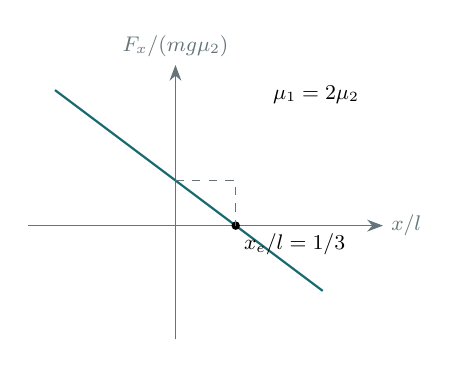
\begin{tikzpicture}[scale=.85,transform shape]
\draw[axis](-2.2,0)--(3.1,0)node[right]{$x/l$};
\draw[axis](0,-1.7)--(0,2.4)node[above]{$F_x/(mg\mu_2)$};
\draw[traj](-1.8,2.025)--(2.2,-.975);
\fill(.9,0)circle(1.8pt)node[below right]{$x_e/l=1/3$};
\draw[guide](0,.675)--(.9,.675)--(.9,0);
\node[above]at(2.1,1.7){$\mu_1=2\mu_2$};
\end{tikzpicture}
\figcaption{变图7.3V4\quad 不同摩擦系数将零合力位置移至中心右侧}
\end{minipage}\end{center}
\item 两轮顶速率均为 $U$，板从 $x=A>0$ 静止释放。初值得 $x=A\cos\Omega t$，因此全过程有 $|\dot x|\leq A\Omega$。变图7.3V5以 $A/l$ 和 $U/(\Omega l)$ 作图，两轮相对滑速始终一正一负要求落在斜线上方。结合正压力和覆盖条件，
\[
A<\min\left(l,\frac{U}{\Omega},\frac{L_b}{2}-l\right).
\]
图中阴影表示前两个严格不等式的共同范围，板长再给出一条相应的竖直上限。
\begin{center}\begin{minipage}{.98\linewidth}\centering
\begin{tikzpicture}[scale=.85,transform shape]
\draw[axis](0,0)--(6.1,0)node[right]{$A/l$};
\draw[axis](0,0)--(0,3.6)node[above]{$U/(\Omega l)$};
\fill[accent!13](0,0)--(3.1,1.86)--(3.1,3.1)--(0,3.1)--cycle;
\draw[traj](0,0)--(5,3);
\draw[object,dashed](3.1,0)--(3.1,3.2)node[above]{$A/l=1$};
\node at(1.4,2.5){固定滑动方向};
\node[right]at(4,1.65){$U=A\Omega$};
\end{tikzpicture}
\figcaption{变图7.3V5\quad 相对滑速给斜线限制，正压力再限定振幅小于半轮距}
\end{minipage}\end{center}
\item 两轮改成背向转动，在持续滑动的阶段两摩擦均反向。由同一载荷差得到
\[
m\ddot x=\mu(N_2-N_1)=\frac{\mu mg}{l}x,\qquad
x=x_i\cosh\Omega t+\frac{v_i}{\Omega}\sinh\Omega t.
\]
变图7.3V6的合力直线斜率为正。若 $x_i>0,v_i=0$，板向右偏移后继续向右加速。该解适用于两压力为正、板覆盖两轮、相对滑动保持图示方向的过程。
\begin{center}\begin{minipage}{.98\linewidth}\centering
\begin{tikzpicture}[scale=.85,transform shape]
\draw[axis](-2.4,0)--(2.4,0)node[right]{$x/l$};
\draw[axis](0,-1.9)--(0,2.1)node[above]{$F_x/(\mu mg)$};
\draw[traj](-1.7,-1.7)--(1.7,1.7);
\draw[force](.9,-.4)--(1.8,-.4);
\draw[force](-.9,.4)--(-1.8,.4);
\node[above left]at(-.6,1.5){背向转动};
\end{tikzpicture}
\figcaption{变图7.3V6\quad 背向转动时，净力与偏移同向}
\end{minipage}\end{center}
\end{enumerate}


\Needspace{18\baselineskip}

\pdfbookmark[2]{第 4 题 地球贯通隧道中的简谐运动}{q4}

\section*{第 4 题\quad 地球贯通隧道中的简谐运动}

\tagline{M-07-04}

牛顿曾证明:一个均匀球壳,对球壳内物质的万有引力为零,而对球壳外物质的万有引

力不为零,并且其作用就相当于球壳的质量都集中到球心那样(参看力学第三章题11).如图所示,设想沿地球直径开凿一条贯通地球的隧道,将一小球从洞口由静止释放,试求小球到达隧道另一洞口所用的时间.已知地球的半径为\(R\),质量为\(M\),设地球的质量均匀分布.

忽略地球自转、空气阻力及开凿对质量分布的影响。

\begin{center}\begin{minipage}{\linewidth}\centering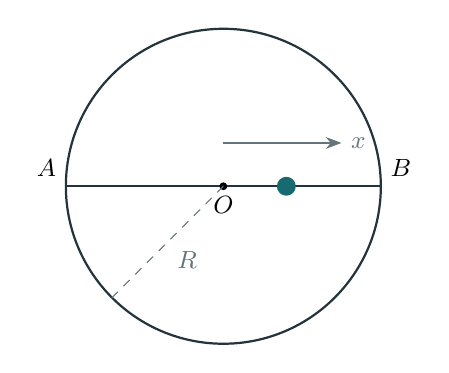
\begin{tikzpicture}[line cap=round,line join=round,spring/.style={decorate,decoration={coil,aspect=.45,segment length=4pt,amplitude=3pt},thick}]\draw[object] (0,0) circle (2);\draw[object] (-2,0)--(2,0);\fill[accent] (.8,0) circle (.12);\fill (0,0) circle (.05);\draw[axis] (0,.55)--(1.5,.55) node[right] {$x$};\node[below] at (0,0) {$O$};\node[above left] at (-2,0) {$A$};\node[above right] at (2,0) {$B$};\draw[guide] (0,0)--(-1.414213562,-1.414213562) node[midway,below right] {$R$};\end{tikzpicture}\figcaption{图 7.4}\end{minipage}\end{center}

\Needspace{5\baselineskip}

\pdfbookmark[3]{题型定位}{q4-h0}

\subsection*{题型定位}

由均匀球内部引力建立简谐方程，再从释放初值求首次到达另一洞口的时间。任意弦的情形把总引力投影到隧道方向。

\Needspace{5\baselineskip}

\pdfbookmark[3]{知识点}{q4-h1}

\subsection*{知识点}

外侧完整球壳对内部质点合引力为零，内侧包围质量为 $M(r)=Mr^3/R^3$。内部引力矢量为 $-GMm\boldsymbol r/R^3$，沿任意弦的回复系数相同。端到端释放对应半周期。


\Needspace{5\baselineskip}

\pdfbookmark[3]{物理图像}{q4-h2}

\subsection*{物理图像}

解图7.4A中右洞口释放后，小球朝地心加速，过地心时速度最大，再向左洞口减速。解图7.4B中弦中点 $H$ 是沿隧道的平衡点，光滑壁支持力抵消横向引力。


\Needspace{5\baselineskip}

\pdfbookmark[3]{解题入口}{q4-h3}

\subsection*{解题入口}

用包围质量和球壳定理写有符号引力 $F_x=-GMmx/R^3$，由 $x(0)=R,\dot x(0)=0$ 得到余弦运动。对 $x=-R$ 取第一次到达的正根 $\omega t=\pi$。

\Needspace{5\baselineskip}

\pdfbookmark[3]{标准解法}{q4-h4}

\subsection*{标准解法}

\begin{center}\begin{minipage}{\linewidth}\centering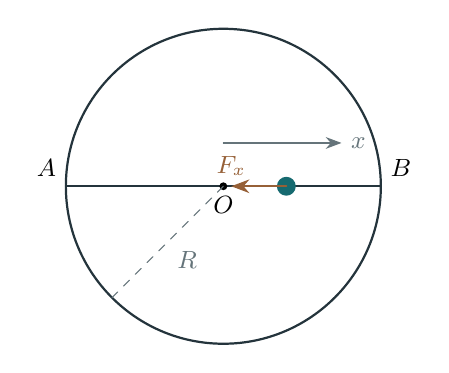
\begin{tikzpicture}[line cap=round,line join=round,spring/.style={decorate,decoration={coil,aspect=.45,segment length=4pt,amplitude=3pt},thick}]\draw[object] (0,0) circle (2);\draw[object] (-2,0)--(2,0);\fill[accent] (.8,0) circle (.12);\fill (0,0) circle (.05);\draw[axis] (0,.55)--(1.5,.55) node[right] {$x$};\node[below] at (0,0) {$O$};\node[above left] at (-2,0) {$A$};\node[above right] at (2,0) {$B$};\draw[guide] (0,0)--(-1.414213562,-1.414213562) node[midway,below right] {$R$};\draw[force] (.8,0)--(.1,0) node[above] {$F_x$};\end{tikzpicture}\figcaption{解图 7.4A}\end{minipage}\end{center}
在地球内部，半径 $r$ 以内的质量为
\[M(r)=\frac{M}{4\pi R^3/3}\frac{4\pi r^3}{3}=M\frac{r^3}{R^3}.\]
外侧球壳的合引力为零。以球心为原点，隧道坐标 $x$ 为有符号量，球受力为
\[F_x=-\frac{GMm}{R^3}x,\qquad
\ddot x+\frac{GM}{R^3}x=0.\]
解图7.4A的力箭头始终指向球心，力的大小与偏心距离成正比；取右洞口$B$为释放处。由 $x(0)=R$、$\dot x(0)=0$，
\[x(t)=R\cos(\omega t),\quad\omega=\sqrt{GM/R^3},\quad
T=2\pi\sqrt{R^3/(GM)}.\]
到另一洞口 $x=-R$ 是第一次达到另一端点，耗时半周期：
\[\boxed{t_{\text{穿越}}=\pi\sqrt{\frac{R^3}{GM}}=\pi\sqrt{\frac R{g_s}},\qquad g_s=GM/R^2.}\]
由能量求得球心速率为 $v_{\max}=\omega R=\sqrt{GM/R}$。地表圆轨道速度也是该值，走半圆的时间 $\pi R/v_{\max}$ 与穿越时间相同；圆周运动投影到直径即为此简谐轨迹。这一等时关系由均匀密度下的线性引力和非旋转模型给出。
若把隧道改为距地心 $b<R$ 的任意弦，以弦中点为坐标原点，则 $\mathbf r=x\hat{\mathbf e}_x+b\hat{\mathbf e}_b$。球内引力的向量式为 $\mathbf F=-m\omega^2\mathbf r$，沿弦仍有 $F_x=-m\omega^2x$；壁的支持力抵消横向分量，大小 $m\omega^2b$，不做功。两洞口坐标为 $x=\pm\sqrt{R^2-b^2}$，振幅改为 $\sqrt{R^2-b^2}$，频率与端到端的半周期不变，最大速度却随弦长减小。解图7.4B把沿弦分量与横向分量分别画出。
\subsubsection*{半径与有符号隧道坐标的区别}
解图7.4A取右洞口$B$为释放处，$x(0)=R$。
半径$r=|x|\geq0$用于计算球内包围质量，
而运动方程用可正可负的$x$，过球心后无需重设正方向。
先由均匀密度逐项消去体积因子，
\[
\rho=\frac{M}{4\pi R^3/3},\qquad
M(r)=\rho\frac{4\pi r^3}{3}=M\frac{r^3}{R^3}.
\]
外侧每一完整球壳对内部小球的合引力都为零，
内侧球体的作用等效于其质量集中在球心。
在$r>0$处，
\[
\boldsymbol F=-\frac{GmM(r)}{r^3}\boldsymbol r
=-\frac{Gm}{r^3}\frac{Mr^3}{R^3}\boldsymbol r
=-\frac{GMm}{R^3}\boldsymbol r.
\]
约去 $r^3$ 后，引力与位矢成正比，在 $r=0$ 连续取零。
沿直径投影再除以$m$，得到$\ddot x+\omega^2x=0$。
这里均匀密度使 $M(r)/r^3=M/R^3$ 成为常量，从而产生线性回复力。

\subsubsection*{从一侧洞口到地心和另一侧洞口的时间}
齐次方程的一般解为$C_1\cos\omega t+C_2\sin\omega t$。
释放条件分别给$C_1=R$、$\omega C_2=0$，故$x=R\cos\omega t$。
第一次到达另一洞口要求$\cos\omega t=-1$，
最小正解为$\omega t=\pi$。地心在两个洞口之间，第一次到地心的时刻为$\pi/(2\omega)$，再经过同样长的时间到另一侧洞口。
在两端，速度为零而加速度朝地心；在地心，速度最大而加速度为零。

引力在直径上的势能差为
\[
U(x)-U(0)=\int_0^x m\omega^2\xi\dd\xi
=\frac12m\omega^2x^2.
\]
以洞口初态作能量常数，
\[
\frac12m\dot x^2+\frac12m\omega^2x^2
=\frac12m\omega^2R^2,
\qquad \dot x=-\omega\sqrt{R^2-x^2}.
\]
负号对应从右洞口向左运动。
用上面的速度将时间写成位移积分，从右侧洞口$R$积到左侧洞口$-R$：
\[
t=\int_R^{-R}\frac{-\dd x}{\omega\sqrt{R^2-x^2}}
=\frac1\omega\left[\arcsin\frac xR\right]_{-R}^{R}
=\frac\pi\omega.
\]
在两端附近，速度按到端点距离的平方根减小。因此时间被积函数虽在端点发散，积分仍收敛。
球心速率$\omega R$与地表圆轨道速率相同，
圆轨道的半圈时间因此也为$\pi/\omega$。
两种运动在直径上的坐标满足同一方程和同一初值，因此投影轨迹相同。

\subsubsection*{任意弦的力分解及模型范围}
解图7.4B取弦中点为$H$，$OH=b$，
沿弦坐标为$x$；相对球心的距离满足$r^2=x^2+b^2$。
\begin{center}\begin{minipage}{\linewidth}\centering
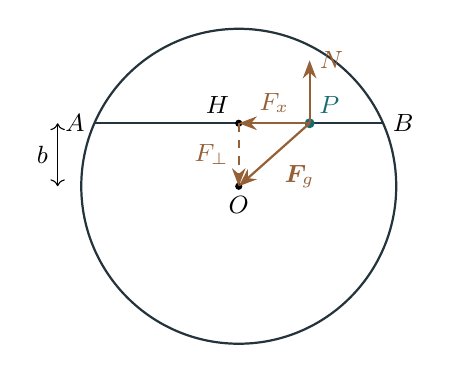
\begin{tikzpicture}[font=\small]
\draw[object](0,0)circle(2);
\draw[object](-1.833030278,.8)--(1.833030278,.8);
\fill(0,0)circle(1.3pt)node[below]{$O$};
\fill(0,.8)circle(1.3pt)node[above left]{$H$};
\fill[accent](.9,.8)circle(1.8pt)node[above right]{$P$};
\draw[force](.9,.8)--(0,0)node[midway,below right]{$\boldsymbol F_g$};
\draw[force](.9,.8)--(0,.8)node[midway,above]{$F_x$};
\draw[force,dashed](0,.8)--(0,0)node[midway,left]{$F_\perp$};
\draw[force](.9,.8)--(.9,1.6)node[right]{$N$};
\draw[<->](-2.3,0)--(-2.3,.8)node[midway,left]{$b$};
\node[left]at(-1.833030278,.8){$A$};\node[right]at(1.833030278,.8){$B$};
\end{tikzpicture}
\figcaption{解图7.4B\quad 弦隧道变式；沿弦回复力指向$H$，横向引力由光滑壁的支持力抵消。}
\end{minipage}\end{center}
球内引力为$-m\omega^2\boldsymbol r$，
两个分量分别是$F_x=-m\omega^2x$与$F_\perp=-m\omega^2b$。
光滑壁给$N=m\omega^2b$，其方向与沿弦速度垂直，不做功。
所以弦的半长虽变为$A=\sqrt{R^2-b^2}$，
时间积分仍是$\int_{-A}^{A}\dd x/[\omega\sqrt{A^2-x^2}]=\pi/\omega$。
行程 $2A$ 与最大速率 $\omega A$ 均按半弦长缩放，所以比值与 $A$ 无关。

均匀密度、忽略自转与阻力、隧道足够窄而不改变球体质量分布，
是上述理想模型的条件。
进入球面时取 $t=0$，令入球位置的有向隧道坐标为 $x_i$、沿隧道的有向速度为 $u_i$。回到球面的这段球内运动可写成 $x=x_i\cos\omega t+(u_i/\omega)\sin\omega t$，其中随时有 $r\leq R$。


\Needspace{5\baselineskip}

\pdfbookmark[3]{关键洞察}{q4-h5}

\subsection*{关键洞察}

均匀密度使内部引力的每个笛卡尔分量都与对应坐标成正比。换一条弦后，沿弦的平衡点和振幅改变，回复斜率保持 $-GMm/R^3$，所以不同弦具有相同的端到端静止释放时间。


\Needspace{5\baselineskip}

\pdfbookmark[3]{易错点}{q4-h6}

\subsection*{易错点}

\begin{itemize}
\item $r=|\boldsymbol r|$ 用于包围质量，隧道坐标 $x$ 则带方向。
\item 地表 $g_s$ 只给洞口处的引力加速度大小，地心处引力为零。
\item 从洞口到地心为四分之一周期，到另一洞口为半周期。
\end{itemize}


\Needspace{5\baselineskip}

\pdfbookmark[3]{课堂讲解建议}{q4-h7}

\subsection*{课堂讲解建议}

指着解图7.4A，先以球壳定理和均匀密度求包围质量，再让学生写出左右两侧共用的有符号受力式。沿轨迹依次标出速度和加速度，明确洞口、地心对应的相位。

在解图7.4B取两个不同 $x$ 的位置，将总引力分别分解。横向分量由壁力抵消，沿弦分量只含 $x$。再比较变图7.4V2中的两条弦，分别计算行程和最大速率，说明它们按同一比例缩放。最后用变图7.4V6读出弱阻力下首次另一侧转折的位置。


\Needspace{5\baselineskip}

\pdfbookmark[3]{变式训练}{q4-h8}

\subsection*{变式训练}

\begin{enumerate}
\item 从直径洞口静止释放，$x(0)=R,\dot x(0)=0$。简谐方程的解为
\[
x=R\cos\omega t,\qquad \dot x=-R\omega\sin\omega t,\qquad
\omega^2=\frac{GM}{R^3}.
\]
变图7.4V1中，$B$ 到 $O$ 首次对应 $\omega t=\pi/2$，此时速率 $\omega R=\sqrt{GM/R}$；到 $A$ 首次对应 $\omega t=\pi$，速度又归零。因此 $t_{\rm cross}=\pi\sqrt{R^3/(GM)}$。
\begin{center}\begin{minipage}{.98\linewidth}\centering
\begin{tikzpicture}[scale=.85,transform shape]
\draw[axis](0,-1.4)--(6.6,-1.4)node[right]{$\omega t$};
\draw[axis](0,-1.4)--(0,1.6)node[above]{$x/R$};
\draw[traj,domain=0:6.283185,samples=100]plot(\x,{cos(deg(\x))});
\foreach \x/\y/\lab in {0/1/B,1.570796/0/O,3.141593/-1/A}{\fill(\x,\y)circle(1.6pt)node[above right]{$\lab$};}
\node[below]at(1.570796,-1.4){$\pi/2$};\node[below]at(3.141593,-1.4){$\pi$};
\end{tikzpicture}
\figcaption{变图7.4V1\quad 右洞口释放，到另一洞口对应半个周期}
\end{minipage}\end{center}
\item 隧道距地心为 $b<R$。变图7.4V2中，半弦长由直角三角形得到 $A=\sqrt{R^2-b^2}$。以弦中点为原点，沿弦的运动为
\[
\ddot x=-\omega^2x,\qquad x=A\cos\omega t,\qquad v_{\max}=\omega A.
\]
从一洞口静止出发，首次到另一洞口仍取 $\omega t=\pi$。直径与弦的行程比为 $R/A$，最大速率比也为 $R/A$，相同的角频率使端到端时间一致。
\begin{center}\begin{minipage}{.98\linewidth}\centering
\begin{tikzpicture}[scale=.85,transform shape]
\draw[object](0,0)circle(2);
\draw[traj](-2,0)--(2,0);
\draw[traj](-1.6,1.2)--(1.6,1.2);
\draw[guide](0,0)--(0,1.2)node[midway,left]{$b$};
\draw[<->](-1.6,1.8)--(1.6,1.8)node[midway,above]{$2A$};
\node[right]at(2,0){直径};\node[right]at(1.6,1.2){弦};
\fill(0,1.2)circle(1.5pt)node[above right]{$H$};
\end{tikzpicture}
\figcaption{变图7.4V2\quad 弦的行程缩短，最大速率按同一半弦长缩小}
\end{minipage}\end{center}
\item 球半径固定，均匀密度变为 $2\rho$。用总质量与密度关系，
\[
M=\frac{4\pi}3\rho R^3,\quad
\omega^2=\frac{4\pi G\rho}{3},\quad
\omega'=\sqrt2\omega,\quad t'_{\rm cross}=\frac{t_{\rm cross}}{\sqrt2}.
\]
变图7.4V3把密度放大因子推广为 $\rho'/\rho$，纵坐标为穿越时间比。若给定的是质量与半径的另一种改动，应由 $\omega^2=GM/R^3$ 将相应质量、半径代入。
\begin{center}\begin{minipage}{.98\linewidth}\centering
\begin{tikzpicture}[scale=.85,transform shape]
\draw[axis](0,0)--(5.9,0)node[right]{$\rho'/\rho$};
\draw[axis](0,0)--(0,3.1)node[above]{$t'/t$};
\draw[traj,domain=.5:5,samples=70]plot(\x,{1.7/sqrt(\x)});
\fill(1,1.7)circle(1.6pt)node[above right]{$(1,1)$};
\fill(2,1.202082)circle(1.6pt)node[above right]{$(2,1/\sqrt2)$};
\end{tikzpicture}
\figcaption{变图7.4V3\quad 固定球半径时，穿越时间与密度平方根成反比}
\end{minipage}\end{center}
\item 在半长为 $A$ 的弦中点给沿弦初速 $u>0$。图7.4V4的球内解为
\[
x=\frac u\omega\sin\omega t,\qquad
\dot x=u\cos\omega t.
\]
当 $u<\omega A$ 时，第一次转折距中点为 $u/\omega<A$。当 $u=\omega A$ 时，首次到洞口的时刻为 $\pi/(2\omega)$，到达速度为零。若 $u>\omega A$，首次到洞口满足
\[
t_B=\frac1\omega\arcsin\frac{\omega A}{u},\qquad
v_B=\sqrt{u^2-\omega^2A^2}>0 .
\]
最后两式给出到球外运动时的位置和速度初值；球外的引力大小取 $GMm/r^2$。
\begin{center}\begin{minipage}{.98\linewidth}\centering
\begin{tikzpicture}[scale=.85,transform shape]
\draw[axis](0,0)--(5.9,0)node[right]{$\omega t$};
\draw[axis](0,0)--(0,3.1)node[above]{$x/A$};
\draw[guide](0,2)--(5.4,2)node[right]{洞口};
\draw[traj,domain=0:1.570796,samples=60]plot({2.6*\x},{2*sin(deg(\x))});
\draw[object,dashed,domain=0:.98511,samples=60]plot({2.6*\x},{2.4*sin(deg(\x))});
\fill(2.561286,2)circle(1.6pt)node[above left]{$u=1.2\omega A$};
\fill(4.08407,2)circle(1.6pt)node[below right]{$u=\omega A$};
\end{tikzpicture}
\figcaption{变图7.4V4\quad 从弦中点出发，较大初速在非零速度下到达洞口}
\end{minipage}\end{center}
\item 求距球心 $b$ 的光滑隧道壁支持力。变图7.4V5把总引力分成沿弦与垂直弦两支，
\[
F_x=-m\omega^2x,\qquad F_\perp=-m\omega^2b,\qquad N=m\omega^2b.
\]
横向加速度为零，故 $N$ 与横向引力相抵。在同一条弦上，$b$ 固定，支持力大小恒定。支持力垂直沿弦速度，功率 $N\boldsymbol e_\perp\cdot\boldsymbol v=0$。取 $b=0$ 恢复直径隧道的零横向支持力。
\begin{center}\begin{minipage}{.98\linewidth}\centering
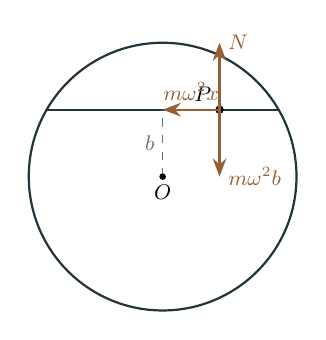
\begin{tikzpicture}[scale=.85,transform shape]
\draw[object](0,0)circle(2);
\draw[object](-1.732051,1)--(1.732051,1);
\fill(.85,1)circle(1.8pt)node[above left]{$P$};
\draw[force](.85,1)--(.85,2)node[right]{$N$};
\draw[force](.85,1)--(.85,0)node[right]{$m\omega^2b$};
\draw[force](.85,1)--(0,1)node[midway,above]{$m\omega^2x$};
\draw[guide](0,0)--(0,1)node[midway,left]{$b$};
\fill(0,0)circle(1.4pt)node[below]{$O$};
\end{tikzpicture}
\figcaption{变图7.4V5\quad 恒定横向引力与支持力抵消，沿弦运动保持不受壁力做功}
\end{minipage}\end{center}
\item 加入线性阻力 $-c\dot x$，取弱阻尼 $\beta=c/(2m)<\omega$，$\omega_d=\sqrt{\omega^2-\beta^2}$。从洞口静止释放，解为
\[
x=Ae^{-\beta t}\left(\cos\omega_dt+\frac{\beta}{\omega_d}\sin\omega_dt\right),
\qquad
\dot x=-\frac{A\omega^2}{\omega_d}e^{-\beta t}\sin\omega_dt.
\]
第二式的正弦第一次再过零给 $t_1=\pi/\omega_d$。代入第一式，
\[
x(t_1)=-Ae^{-\beta\pi/\omega_d},\qquad |x(t_1)|<A.
\]
变图7.4V6取 $\beta/\omega_d=0.15$，首次左侧转折约为 $-0.624A$。此后振动幅度继续衰减，各转折点保持在洞内。图解及弦的比较均采用均匀球、窄隧道和题设的非旋转条件。
\begin{center}\begin{minipage}{.98\linewidth}\centering
\begin{tikzpicture}[scale=.85,transform shape]
\draw[axis](0,-1.4)--(7.4,-1.4)node[right]{$\omega_dt$};
\draw[axis](0,-1.4)--(0,1.5)node[above]{$x/A$};
\draw[traj,domain=0:6.9,samples=110]plot(\x,{exp(-.15*\x)*(cos(deg(\x))+.15*sin(deg(\x)))});
\draw[guide](0,-1)--(6.9,-1)node[right]{另一洞口};
\fill(3.141593,-.624228)circle(1.7pt)node[above]{$-e^{-\beta\pi/\omega_d}$};
\node[below]at(3.141593,-1.4){$\pi$};
\end{tikzpicture}
\figcaption{变图7.4V6\quad 弱阻力下首次反向转折的位置位于洞内}
\end{minipage}\end{center}
\end{enumerate}


\clearpage

\pdfbookmark[2]{第 5 题 斜面上弹簧连接滚动圆柱的振动周期}{q5}

\section*{第 5 题\quad 斜面上弹簧连接滚动圆柱的振动周期}

\tagline{M-07-05}

如图7.5,在倾角为\(\theta\)的斜面上有一劲度系数为\(k\)的弹簧,一端固定,另一端与质量为\(m\)的实心圆柱体的轴连接,圆柱体在斜面上作纯滚动.忽略轴承的摩擦.试求振动周期.

\begin{center}\begin{minipage}{\linewidth}\centering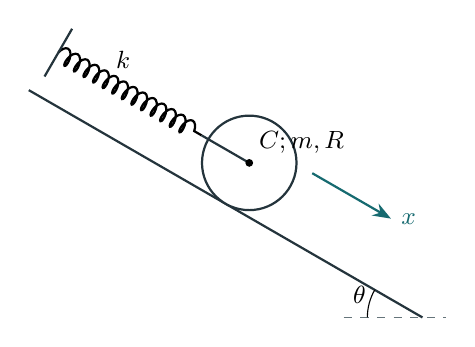
\begin{tikzpicture}[font=\small,spring/.style={decorate,decoration={coil,aspect=.45,segment length=4pt,amplitude=3pt},thick}]
\coordinate(P)at(.5,-.288675135);\coordinate(C)at(.8,.230940108);\coordinate(S)at(-1.624871131,1.630940108);\coordinate(E)at(.193782217,.580940108);
\draw[object](-2,1.154700538)--(3,-1.732050808);\draw[guide](2,-1.732050808)--(3.3,-1.732050808);
\draw[object,fill=white](C)circle(.6);\draw[spring](S)--(E);\draw[object](E)--(C);
\draw[object](-1.799871131,1.327831217)--(-1.449871131,1.934048999);
\fill(C)circle(1.4pt);\node[above right]at(C){$C;m,R$};\node[above]at(-.8,1.3){$k$};
\draw[motion](1.6,.1)--(2.6,-.477350269)node[right]{$x$};
\draw(2.3,-1.732050808)arc(180:150:.7);\node at(2.2,-1.45){$\theta$};
\end{tikzpicture}\figcaption{图 7.5}\end{minipage}\end{center}

\Needspace{5\baselineskip}

\pdfbookmark[3]{题型定位}{q5-h0}

\subsection*{题型定位}

平动与自转折算成单自由度的滚动振动题。重力改变平衡伸长，频率则由弹簧刚度和等效惯性决定。

\Needspace{5\baselineskip}

\pdfbookmark[3]{知识点}{q5-h1}

\subsection*{知识点}

纯滚动；圆柱惯量；摩擦力矩；平衡位移；动能相加；不滑动幅值范围。

无滑约束把自旋角速度与质心速度联系为$|\dot\varphi|=|\dot x|/R$，所以惯性折算为$m+I/R^2$。静摩擦由转动方程给出所需值，临界无滑状态才达到$\mu_sN$。


\Needspace{5\baselineskip}

\pdfbookmark[3]{物理图像}{q5-h2}

\subsection*{物理图像}

以平衡点为原点，回复增量为\(-kx\)。接触摩擦提供角加速度，方向随$x$改变，在平衡点两侧分别向上坡与下坡。

解图7.5A的位移从平衡位置量起，弹簧真实伸长是$x_0+x$。在$x>0$端点，质心加速度向上坡，摩擦却可向下坡；它提供使平动与自转相容的角加速度，方向由滚动约束和力矩共同确定。


\Needspace{5\baselineskip}

\pdfbookmark[3]{解题入口}{q5-h3}

\subsection*{解题入口}

扣除静态\(mg\sin\theta\)，列平动、自转和滚动约束三式。能量法将质心平动与绕心自转动能相加。

先列静态的$kx_0=mg\sin\theta$，再在动态式中减去它，保留增量$-kx$。这一步将重力对平衡的影响与对频率的影响分开，随后用滚动约束消去摩擦和角加速度。


\Needspace{18\baselineskip}

\Needspace{5\baselineskip}

\pdfbookmark[3]{标准解法}{q5-h4}

\subsection*{标准解法}

\begin{center}\begin{minipage}{\linewidth}\centering\begin{tikzpicture}[font=\small]
\coordinate(P)at(.5,-.288675135);\coordinate(C)at(.8,.230940108);
\draw[object](-2,1.154700538)--(3,-1.732050808);\draw[object](C)circle(.6);
\fill(C)circle(1.4pt)node[below left]{$C$};\node[below left]at(P){$P$};
\draw[force](C)--(-1.278460969,1.430940108)node[above left]{$k(x_0+x)$};
\draw[force](C)--(1.579422863,1.580940108)node[right]{$N$};
\draw[force](C)--(.8,-1.569059892)node[below right]{$mg$};
\draw[force](P)--(.933012702,-.538675135)node[right]{$f$};
\node[align=left,anchor=west]at(2,1.4){$x>0$\\$f>0$向下坡};
\end{tikzpicture}\figcaption{解图 7.5A}\end{minipage}\end{center}
取下坡方向为正，$x$ 从圆柱平衡位置量起，弹簧平衡伸长为 $x_0$。静态时摩擦不需提供转矩，故
\[kx_0=mg\sin\theta.\]
任意位移时，解图7.5A中的 $f$ 先按向下坡的有符号量定义。平移、绕心转动和无滑约束分别为
\[m\ddot x=mg\sin\theta-k(x_0+x)+f,
\quad I\beta=fR,\quad\beta=-\ddot x/R.\]
绕心转动与滚动约束联立给
\[f=\frac{I\beta}{R}=-\frac I{R^2}\ddot x.\]
把它代入平动式，相当于同一个质心加速度还须带动转动自由度，故有效惯性增加$I/R^2$。静态的$mg\sin\theta$与$kx_0$相消，剩下的弹簧增量$kx$才提供回复力。解图7.5A中$x>0$时圆柱向上坡加速，所需摩擦却向下坡，以产生相应自旋加速度。

消去 $f,\beta$ 并减掉平衡式：
\[\left(m+\frac I{R^2}\right)\ddot x=-kx.\]
均匀实心圆柱 $I=mR^2/2$，于是
\[\boxed{\omega=\sqrt{\frac{2k}{3m}},\qquad
T=2\pi\sqrt{\frac{3m}{2k}}.}\]
重力只改变平衡伸长，没有改变线性回复系数。摩擦实际为
\[f=-\frac I{R^2}\ddot x=\frac{kx}{3},\]
随 $x$ 改变方向，$x>0$时向下坡，$x<0$时向上坡。振幅 $A$ 需满足 $kA/3\le\mu_smg\cos\theta$ 才能保持纯滚。
能量另解保留转动能：
\[E=\frac12m\dot x^2+\frac12I(\dot x/R)^2+\frac12kx^2
=\frac34m\dot x^2+\frac12kx^2.\]
对时间求导，仍得 $(3m/2)\ddot x+kx=0$。
\subsubsection*{扣除静态平衡后的完整动力学消元}
图7.5中弹簧通过轴承作用于圆柱中心，方向平行于斜面，
所以它不直接产生绕心力矩，也不改变法向支持力$N=mg\cos\theta$。
取下坡平移为正、逆时针自转为正，无滑约束的有符号式为
$\dot\varphi=-\dot x/R$、$\beta=-\ddot x/R$。
静止平衡时$\beta=0$，由$fR=I\beta$得$f=0$，
再从平动平衡求$x_0=mg\sin\theta/k$。

动态的三个方程逐个代入，
\[
f=\frac I R\beta=-\frac I{R^2}\ddot x,
\]
\[
m\ddot x=mg\sin\theta-kx_0-kx-\frac I{R^2}\ddot x,
\]
\[
\left(m+\frac I{R^2}\right)\ddot x
=\underbrace{mg\sin\theta-kx_0}_{0}-kx.
\]
代$I=mR^2/2$，有$\ddot x=-2kx/(3m)$、
$f=-m\ddot x/2=kx/3$。
解图7.5A画$x>0$时的力：弹簧实际力为$k(x_0+x)$，
扣除重力后的增量才是$kx$；受力图应分别标明实际弹力与回复增量。
当$x<0$时$f<0$，摩擦向上坡。

\subsubsection*{两项动能、重力与弹簧势的展开}
质心从平衡点下移$x$，重力势能变化为$-mgx\sin\theta$，
弹簧势能变化为
\[
\frac k2[(x_0+x)^2-x_0^2]=kx_0x+\frac12kx^2.
\]
用$kx_0=mg\sin\theta$，两项线性势能相消，
总有效势只剩$kx^2/2$。
动能则为
\[
\frac12m\dot x^2+\frac12\frac{mR^2}{2}
\frac{\dot x^2}{R^2}=\frac34m\dot x^2.
\]
所以能量求导的完整形式是
\[
0=\frac{\dd E}{\dd t}
=\dot x\left(\frac32m\ddot x+kx\right).
\]
在速度非零的运动段消去$\dot x$得到动力学方程，
转折点处则由方程连续延伸，不在零因子上作除法。

静摩擦对质心平移的功率是$f\dot x$，
对绕心自转的功率为$(fR)\dot\varphi=-f\dot x$，
两者相消，等价于接触材料点相对静止斜面的速度为零。
接触点静止使摩擦总功为零；相加的平动和自转动能共同给出有效惯性。

\subsubsection*{振动初值与纯滚动的可实现范围}
一般初值$x_i,v_i$须同时满足初始无滑自转$\dot\varphi_i=-v_i/R$，
随后
\[
x=x_i\cos\omega t+\frac{v_i}{\omega}\sin\omega t,
\qquad A=\sqrt{x_i^2+(v_i/\omega)^2}.
\]
最大所需静摩擦发生在位移端点，而非速度最大处，
\[
|f|_{\max}=\frac{kA}{3},\qquad
A\leq\frac{3\mu_smg\cos\theta}{k}.
\]
在平衡点$x=0$，质心速率最大，但瞬时角加速度与所需摩擦都为零。
若弹簧可受拉也可受压，$x_0+x$取有符号伸长；
若连接只能拉而会松弛，还须$A\leq x_0$，否则需另分松弛运动段。
增大斜角会增大$x_0$、减小法向载荷及纯滚幅值上限，
却不改变当前模型中的周期。


\Needspace{5\baselineskip}

\pdfbookmark[3]{关键洞察}{q5-h5}

\subsection*{关键洞察}

惯性变成\(m+I/R^2\)。斜角不直接进入频率，却通过支持力决定静摩擦可维持多大的振幅。

静摩擦对静止斜面接触点不做功，但对质心平移和绕心转动的功率可分别非零、相互转移。能量法保留两部分动能，动力学法保留摩擦，二者才会得到同一等效惯性。


\Needspace{5\baselineskip}

\pdfbookmark[3]{易错点}{q5-h6}

\subsection*{易错点}

平动与转动动能分别计算，再用无滑约束相连。轴心弹力对圆心的矩为零，静摩擦提供自转力矩。求得周期后，把最大所需摩擦$kA/3$与$\mu_smg\cos\theta$比较；超过该范围时，按滑动接触另列平动和转动方程。


\Needspace{5\baselineskip}

\pdfbookmark[3]{课堂讲解建议}{q5-h7}

\subsection*{课堂讲解建议}

先比较实心圆柱与薄圆环的动能，再预测哪一个周期较长。
沿图7.5指出弹簧连轴心且平行于斜面；
在解图7.5A区分实际弹力$k(x_0+x)$与扣平衡后的回复增量$kx$。
由静态转矩先求$f=0$，再列$kx_0=mg\sin\theta$。

分别用动力学和能量求周期。
动力学保留摩擦并消去$\beta$，能量展开重力和弹簧势的一次项，
再将质心平动与自旋动能相加。
用$f\dot x+(fR)\dot\varphi=0$解释静摩擦净功为零，
同时说明它仍提供转动所需的力矩。

在两个位移端点画摩擦方向，检查$kA/3\leq\mu_smg\cos\theta$。
再问平衡点处速率最大，为何所需摩擦反而为零：这里加速度与角加速度都为零。
初始角速度不匹配时先分析滑动，单拉连接松弛时也须另分运动段。

逐项比较增大斜角对平衡伸长、周期和允许幅值的影响。
由三个式子分别解释伸长增大、线性周期不变、静摩擦幅值上限下降，
分别对应平衡位置、运动时间尺度与接触可实现幅值这三项物理量。


\Needspace{5\baselineskip}

\pdfbookmark[3]{变式训练}{q5-h8}

\subsection*{变式训练}

\begin{enumerate}
\item 换成薄圆环，弹簧仍连中心且平行斜面。
$I=mR^2$给等效惯性$2m$，故$T=2\pi\sqrt{2m/k}$，
比实心圆柱的$2\pi\sqrt{3m/(2k)}$长。
所需摩擦为$kx/2$，同一允许静摩擦下的振幅上限也须重新计算。
图V1用$\kappa=I/(mR^2)$给出的频率曲线标出圆环与圆柱。圆环的平动式$m\ddot x=-kx+f$和转动式$f=-m\ddot x$联立得$2m\ddot x=-kx$，故$f=kx/2$，幅值还取$A\le2\mu_smg\cos\theta/k$。
\begin{center}\begin{minipage}{.98\linewidth}\centering
\begin{tikzpicture}[scale=.88,transform shape]
\draw[axis](0,0)--(6.7,0)node[right]{$\kappa=I/(mR^2)$};\draw[axis](0,0)--(0,3.4)node[above]{$\omega/\sqrt{k/m}$};
\draw[traj,domain=0:1.5,samples=90]plot({4*\x},{3/sqrt(1+\x)});
\fill(2,2.44949)circle(1.7pt)node[above]{圆柱};\fill(4,2.12132)circle(1.7pt)node[below]{圆环};
\end{tikzpicture}
\figcaption{变图7.5V1\quad 转动惯量增大使滚动振动频率降低。}
\end{minipage}\end{center}
\item 换成均匀实心球。
$I=2mR^2/5$，故等效惯性$7m/5$，
$T=2\pi\sqrt{7m/(5k)}$，所需摩擦为$2kx/7$。
弹力通过球心时，其绕心矩为零；偏心连接时将弹力矩一并加入转动方程。
图V2中球心的增量弹力$-kx$不产生绕心力矩，接触点的$fR=I\beta$与$\beta=-\ddot x/R$给$f=-(2m/5)\ddot x$。代回平动式，得到$(7m/5)\ddot x=-kx$，从而$f=2kx/7$，幅值上限为$7\mu_smg\cos\theta/(2k)$。
\begin{center}\begin{minipage}{.98\linewidth}\centering
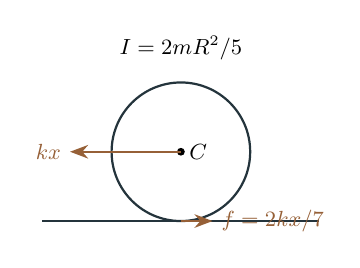
\begin{tikzpicture}[scale=.88,transform shape]
\draw[object](-2,0)--(2,0);\draw[object](0,1)circle(1);\fill(0,1)circle(1.6pt)node[right]{$C$};
\draw[force](0,1)--(-1.6,1)node[left]{$kx$};\draw[force](0,0)--(.45714,0)node[right]{$f=2kx/7$};
\node[above]at(0,2.2){$I=2mR^2/5$};
\end{tikzpicture}
\figcaption{变图7.5V2\quad 沿斜面坐标展开的球体增量受力，摩擦提供转动力矩。}
\end{minipage}\end{center}
\item 只改变斜角$\theta$。
静态伸长$x_0=mg\sin\theta/k$随角度改变，
小振动频率仍由$m+I/R^2$与$k$决定。
支持力$mg\cos\theta$减小会降低可维持的静摩擦和允许振幅；
如连接只能受拉，还应检查最小伸长是否保持张紧。
图V3把两个长度分别归一。$\hat x_0=kx_0/(mg)=\sin\theta$，$\hat A=kA_{\max}/(3\mu_smg)=\cos\theta$。若仅受拉，最小伸长$x_0-A$取非负，最终幅值取两项上限中较小者。
\begin{center}\begin{minipage}{.98\linewidth}\centering
\begin{tikzpicture}[scale=.88,transform shape]
\draw[axis](0,0)--(6.4,0)node[right]{$\theta$};\draw[axis](0,0)--(0,3.5)node[above]{归一化长度};
\draw[traj,domain=0:85,samples=90]plot({\x/15},{3*sin(\x)});
\draw[object,color=warm,domain=0:85,samples=90]plot({\x/15},{3*cos(\x)});
\node[right]at(5.7,3){$\hat x_0$};\node[right]at(5.7,.26){$\hat A$};
\end{tikzpicture}
\figcaption{变图7.5V3\quad 增大斜角使平衡伸长增大，允许幅值降低。}
\end{minipage}\end{center}
\item 实心圆柱的幅值条件。
平动和自转式消元得$f=kx/3$，两端所需摩擦最大值$kA/3$。
无滑要求$kA/3\le\mu_smg\cos\theta$，
故$A\le3\mu_smg\cos\theta/k$。摩擦方向随$x$变号，
仅在最大所需值等于$\mu_sN$的临界幅值处达到摩擦上限。
图V4横轴$\xi=kx/(3\mu_sN)$，纵轴$f/(\mu_sN)$，两者相等。端点 $|\xi|=1$ 对应最大静摩擦。过平衡点时平动和转动的加速度都为零，故 $f=0$；此时圆柱的平动速率与自转角速率达到最大。
\begin{center}\begin{minipage}{.98\linewidth}\centering
\begin{tikzpicture}[scale=.88,transform shape]
\draw[axis](-3.5,0)--(3.5,0)node[right]{$\xi$};\draw[axis](0,-2.6)--(0,2.6)node[above]{$f/(\mu_sN)$};
\draw[traj](-2.3,-2.3)--(2.3,2.3);\draw[guide](-3,2.3)--(3,2.3);\draw[guide](-3,-2.3)--(3,-2.3);
\node[below]at(2.3,0){$1$};\node[above]at(-2.3,0){$-1$};
\end{tikzpicture}
\figcaption{变图7.5V4\quad 摩擦随位移线性变号，两条虚线给静摩擦上限。}
\end{minipage}\end{center}
\item 在平衡点给向下坡速度$u$并匹配无滑角速度。
此时$x(0)=0$、$\dot x(0)=u$，
$x=(u/\omega)\sin\omega t$、$A=|u|/\sqrt{2k/(3m)}$。
若初始自旋不满足接触点静止，则先有滑动阶段，须先求其冲量及耗散，
滑动结束后，以当时相容的平动、自转初值开始纯滚动阶段。
图V5按初值画出相轨道$(x/A)^2+(\dot x/u)^2=1$，起点为$(0,1)$。振幅代回摩擦条件得到$|u|\le\omega\,3\mu_smg\cos\theta/k$；相应初自旋为$-u/R$。
\begin{center}\begin{minipage}{.98\linewidth}\centering
\begin{tikzpicture}[scale=.88,transform shape]
\draw[axis](-2.6,0)--(2.6,0)node[right]{$x/A$};\draw[axis](0,-2.6)--(0,2.6)node[above]{$\dot x/u$};\draw[traj](0,0)circle(2);
\fill(0,2)circle(1.8pt)node[above left]{初态};\draw[motion,domain=15:45,samples=25]plot({2*sin(\x)},{2*cos(\x)});
\end{tikzpicture}
\figcaption{变图7.5V5\quad 匹配无滑初速度时，相轨道由平衡点的速度端起始。}
\end{minipage}\end{center}
\item 刚度增为$4k$，并使新的静态平衡条件成立。
频率加倍、周期减半；同幅值的所需摩擦变为4倍，
允许纯滚动幅值上限降为四分之一。
保持原振幅时所需摩擦增大；若超过摩擦上限，则进入滑动阶段。
图V6用比值表示参数变化：$x_{0,\rm new}/x_0=1/4$、$\omega_{\rm new}/\omega=2$、$A_{\max,\rm new}/A_{\max}=1/4$。这些分别来自静态式、惯性不变的频率式和摩擦上限式。
\begin{center}\begin{minipage}{.98\linewidth}\centering
\begin{tikzpicture}[scale=.88,transform shape]
\draw[axis](0,0)--(7.3,0);\draw[axis](0,0)--(0,3)node[above]{新值/旧值};
\fill[accent!30](1,0)rectangle(2,.35);\fill[accent!30](3,0)rectangle(4,2.8);\fill[accent!30](5,0)rectangle(6,.35);
\node[below]at(1.5,0){$x_0$};\node[below]at(3.5,0){$\omega$};\node[below]at(5.5,0){$A_{\max}$};
\node[above]at(1.5,.35){$1/4$};\node[above]at(3.5,2.8){$2$};\node[above]at(5.5,.35){$1/4$};
\end{tikzpicture}
\figcaption{变图7.5V6\quad 刚度四倍时，平衡伸长、频率与允许幅值各按所示比例改变。}
\end{minipage}\end{center}\end{enumerate}
统一写$I=\kappa mR^2$，有$\omega^2=k/[m(1+\kappa)]$，
$f=\kappa kx/(1+\kappa)$，从而
$A\le(1+\kappa)\mu_smg\cos\theta/(\kappa k)$。
分别代$\kappa=1/2,1,2/5$给出圆柱、圆环、球各自的周期与摩擦约束；
静摩擦总功率为零仍需接触点相对静止这一条件。


\clearpage

\pdfbookmark[2]{第 6 题 直角均匀杆连弹簧的微小摆动}{q6}

\section*{第 6 题\quad 直角均匀杆连弹簧的微小摆动}

\tagline{M-07-06}

如图,直角形均匀细杆的水平杆长为\(l\)、质量为\(m\),竖直杆长为\(2l\)、质量为\(2m\),细杆可绕拐角处的固定轴\(O\)无摩擦地转动.水平杆的一端与劲度系数为\(k\)的弹簧相连,平衡时水平杆呈

水平状态,竖直杆竖直下垂．试求微小摆动的周期．

弹簧上端固定在水平杆端点的正上方；只计算微小摆动的一阶回复力矩。

\begin{center}\begin{minipage}{\linewidth}\centering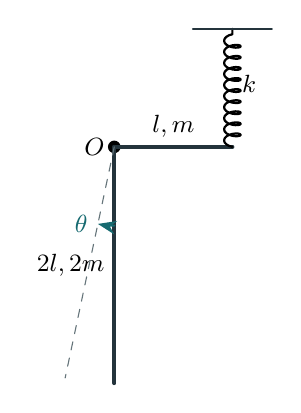
\begin{tikzpicture}[line cap=round,line join=round,spring/.style={decorate,decoration={coil,aspect=.45,segment length=4pt,amplitude=3pt},thick}]\fill (0,0) circle (.08);\node[left] at (0,0) {$O$};\draw[object,line width=1.5pt] (0,0)--(1.5,0);\draw[object,line width=1.5pt] (0,0)--(0,-3);\draw[spring] (1.5,0)--(1.5,1.5);\draw[object] (1,1.5)--(2,1.5);\node[right] at (1.5,.8) {$k$};\node[above] at (.75,0) {$l,m$};\node[left] at (0,-1.5) {$2l,2m$};\draw[guide] (0,0)--(-.623735073,-2.934442802);\draw[motion] (0,-1) arc[start angle=-90,end angle=-102,radius=1] node[left] {$\theta$};\end{tikzpicture}\figcaption{图 7.6}\end{minipage}\end{center}

\Needspace{5\baselineskip}

\pdfbookmark[3]{题型定位}{q6-h0}

\subsection*{题型定位}

非对称直角刚体的弹簧预载和微小摆动题。静态矩确定弹簧预伸长；在该平衡附近，各力矩的一阶变化共同给出角度刚度。

\Needspace{5\baselineskip}

\pdfbookmark[3]{知识点}{q6-h1}

\subsection*{知识点}

两杆端点惯量；质心；预载平衡；端点几何位移；力矩小角展开。

转矩线性化保留小角的一阶项，转动惯量则关于固定铰点$O$求和。平衡预拉力消去常数矩，不会消去长臂重力产生的角度刚度$2mgl$。


\Needspace{5\baselineskip}

\pdfbookmark[3]{物理图像}{q6-h2}

\subsection*{物理图像}

水平臂长l、质量m，下垂臂长2l、质量2m。水平端向下移动\(l\theta\)使拉力增加，下垂臂质心横移产生重力回复力矩。

解图7.6A中短臂端点的竖直位移为$l\theta$的一阶量，水平移动为二阶量。长臂质心距铰点为$l$，因此它的重力臂是$l\sin\theta$，其中$l$是长臂质心到轴的距离。


\Needspace{5\baselineskip}

\pdfbookmark[3]{解题入口}{q6-h3}

\subsection*{解题入口}

先求弹簧静态拉力，随后展开总力矩。每杆绕端点惯量为质量乘该杆长度平方的三分之一，转轴固定于杆端$O$，两臂均按杆端惯量计算。

先把弹簧力写成$k(x_0+l\theta)$，将静态项和增量项分开。在矩方程中逐项标阶，再代入$I_O=3ml^2$；若一开始把$\sin\theta$置零，会把真正的重力回复机制删掉。


\Needspace{18\baselineskip}

\Needspace{5\baselineskip}

\pdfbookmark[3]{标准解法}{q6-h4}

\subsection*{标准解法}

\begin{center}\begin{minipage}{\linewidth}\centering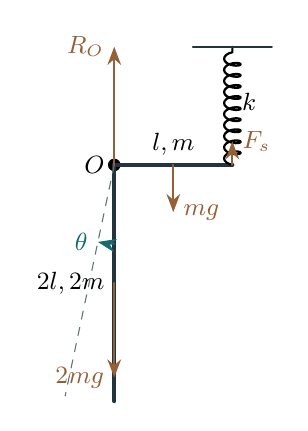
\begin{tikzpicture}[line cap=round,line join=round,spring/.style={decorate,decoration={coil,aspect=.45,segment length=4pt,amplitude=3pt},thick}]\fill (0,0) circle (.08);\node[left] at (0,0) {$O$};\draw[object,line width=1.5pt] (0,0)--(1.5,0);\draw[object,line width=1.5pt] (0,0)--(0,-3);\draw[spring] (1.5,0)--(1.5,1.5);\draw[object] (1,1.5)--(2,1.5);\node[right] at (1.5,.8) {$k$};\node[above] at (.75,0) {$l,m$};\node[left] at (0,-1.5) {$2l,2m$};\draw[guide] (0,0)--(-.623735073,-2.934442802);\draw[motion] (0,-1) arc[start angle=-90,end angle=-102,radius=1] node[left] {$\theta$};\draw[force] (1.5,0)--(1.5,.3)node[right]{$F_s$};\draw[force] (.75,0)--(.75,-.6) node[right] {$mg$};\draw[force] (0,-1.5)--(0,-2.7) node[left] {$2mg$};\draw[force](0,0)--(0,1.5)node[left]{$R_O$};\end{tikzpicture}\figcaption{解图 7.6A}\end{minipage}\end{center}
以顺时针微转角 $\theta$ 为正。平衡时水平杆端点受弹簧向上的力，抵消该臂重力矩：
\[kx_0l=mg\frac l2,\qquad x_0=\frac{mg}{2k}.\]
转动后，水平臂端点向下位移 $x=l\sin\theta=l\theta+O(\theta^3)$；水平位移为二阶，弹簧方向偏离竖直也只产生二阶及更高修正。到一阶时，合矩为
\[\begin{aligned}
\tau&=mg\frac l2\cos\theta-k(x_0+x)l\cos\theta-2mgl\sin\theta+O(\theta^3)\\
&=-(kl^2+2mgl)\theta+O(\theta^3).
\end{aligned}\]
\Needspace{11\baselineskip}解图7.6A中竖直长臂的质心距 $O$ 为 $l$，故其重力回复矩为 $-2mgl\theta$，其力臂从轴量至长臂中点。两臂的转动惯量相加：
\[I_O=\frac13ml^2+\frac13(2m)(2l)^2=3ml^2.\]
于是
\[\ddot\theta+\frac{kl+2mg}{3ml}\theta=0,\qquad
\boxed{T=2\pi\sqrt{\frac{3ml}{kl+2mg}}.}\]
在同一平衡附近展开势能，也能求出角度刚度。令平衡时势能为零，短臂质心向下移动$(l/2)\sin\theta$，长臂质心升高$l(1-\cos\theta)$，弹簧额外伸长在所保留阶次为$l\sin\theta$。因此
\[\begin{aligned}
\Delta U={}&\frac k2[(x_0+l\sin\theta)^2-x_0^2]
-\frac{mgl}{2}\sin\theta+2mgl(1-\cos\theta)+O(\theta^4)\\
={}&\frac12kl^2\sin^2\theta+2mgl(1-\cos\theta)+O(\theta^4)
\simeq\frac12(kl^2+2mgl)\theta^2.
\end{aligned}\]
第二行使用了$kx_0=mg/2$，显式显示预拉力的一次势能项与短臂重力项相消。再除以转动惯量$3ml^2$，得到与力矩法相同的$\omega^2$。

小角近似应取 $\sin\theta\simeq\theta$；若直接令它为零，会删去竖直臂的有效回复矩。弹簧静态预拉力与短臂重力的常数矩相抵，额外伸长和长臂重力共同决定频率。
\subsubsection*{固定弹簧的实际几何及近似阶次}
解图7.6B以$O$为原点，向右、向上为坐标正向，
顺时针$\theta>0$。短臂端点和弹簧固定点分别为
\[
A=(l\cos\theta,-l\sin\theta),\qquad S=(l,H),
\]
其中$H>0$是平衡时的实际弹簧长度。
端点向下位移$x=l\sin\theta$，水平位移$l(\cos\theta-1)$从二阶开始。
真实弹簧长度由两点距离确定：
\[
\ell_s=\sqrt{l^2(1-\cos\theta)^2+(H+l\sin\theta)^2}
=\sqrt{H^2+2Hl\sin\theta+2l^2(1-\cos\theta)}.
\]
其相对平衡长度的变化为
\[
\delta\ell=\ell_s-H
=l\sin\theta+\frac{l^2}{8H}\theta^4+O(\theta^5).
\]
因此求一阶力矩或二阶势能时，可用$l\sin\theta$替代真实伸长变化；
计算有限角度运动或高阶频率修正时，须恢复完整长度。
弹簧方向偏转从$\theta^2$开始，配合端点高度的一阶变化，
对力矩的修正从三阶开始，不改变本题的线性周期。

\begin{center}\begin{minipage}{\linewidth}\centering
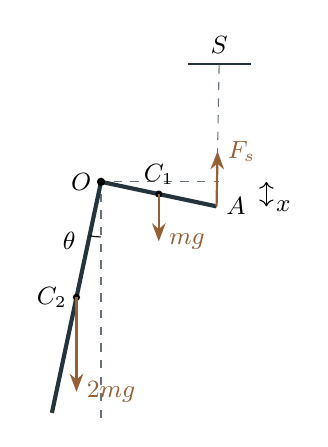
\begin{tikzpicture}[font=\small]
\coordinate(O)at(0,0);\coordinate(A)at(1.467221401,-.311867536);\coordinate(B)at(-.623735073,-2.934442802);\coordinate(S)at(1.5,1.5);
\draw[guide](0,-3)--(O)--(1.5,0);\draw[object,line width=1.5pt](A)--(O)--(B);
\draw[guide](A)--(S);\draw[object](1.1,1.5)--(1.9,1.5);
\fill(O)circle(1.5pt)node[left]{$O$};\node[right]at(A){$A$};\node[above]at(S){$S$};
\fill(.733610700,-.155933768)circle(1.3pt)node[above]{$C_1$};
\fill(-.311867536,-1.467221401)circle(1.3pt)node[left]{$C_2$};
\draw[force](.733610700,-.155933768)--++(0,-.6)node[right]{$mg$};
\draw[force](-.311867536,-1.467221401)--++(0,-1.2)node[right]{$2mg$};
\draw[force](A)--++(.012661668,.699885478)node[right]{$F_s$};
\draw[<->](2.1,0)--(2.1,-.311867536)node[right]{$x$};
\draw(0,-.7)arc(-90:-102:.7);\node[left]at(-.2,-.75){$\theta$};
\end{tikzpicture}
\figcaption{解图7.6B\quad 示例$\theta=12^\circ$；两臂长度不变，弹簧方向由固定点$S$与活动端$A$确定。}
\end{minipage}\end{center}

\subsubsection*{由真实势能求二阶回复系数}
两臂质心分别在$A/2$和长臂中点，
短臂重力势变化为$-mgl\sin\theta/2$，
长臂重力势变化为$2mgl(1-\cos\theta)$。
把真实伸长$\delta\ell$代入弹簧势能，
\[
\Delta U=\frac k2[(x_0+\delta\ell)^2-x_0^2]
-\frac{mgl}{2}\sin\theta+2mgl(1-\cos\theta).
\]
到足够确定二次项的精度，先展开平方：
\[
\Delta U=
\left(kx_0-\frac{mg}{2}\right)l\sin\theta
+\frac12kl^2\sin^2\theta+2mgl(1-\cos\theta)+O(\theta^4).
\]
括号由静态平衡为零，余下
\[
\Delta U=\frac12(kl^2+2mgl)\theta^2+O(\theta^4),
\qquad \tau=-\frac{\dd U}{\dd\theta}
=-(kl^2+2mgl)\theta+O(\theta^3).
\]
短臂重力的低阶项被预载抵消，长臂重力的二阶势能仍为$mgl\theta^2$，
所以它对角度刚度的贡献是$2mgl$。

惯量可按两个独立杆端积分，
\[
I_1=\frac ml\int_0^l r^2\dd r=\frac13ml^2,
\qquad I_2=\frac{2m}{2l}\int_0^{2l}r^2\dd r=\frac83ml^2.
\]
相加为$3ml^2$，再与角度刚度相除，
\[
\omega^2=\frac{kl^2+2mgl}{3ml^2}
=\frac{k}{3m}+\frac{2g}{3l}.
\]
两项量纲均为$1/\mathrm s^2$；质量、惯量或刚度任一处漏长臂，都会破坏这一分解。
若改变$k$或杆质量后仍使用此式，须同时保持题设的水平、下垂平衡构型，
相应调整预伸长；固定自然长和固定点而任意改参数时，平衡位置一般会改变。


\Needspace{5\baselineskip}

\pdfbookmark[3]{关键洞察}{q6-h5}

\subsection*{关键洞察}

预载与水平臂重力的常量力矩相消，但弹力增量和下垂臂重力仍贡献回复项。小角度的$\sin\theta\simeq\theta$保留长臂重力的一阶变化。

同样的小角模型中，一项重力矩是平衡时的常数，另一项重力矩是一阶回复项。判断是否影响频率，要看对$\theta$的导数，再将各项导数与静态矩分别列出。


\Needspace{5\baselineskip}

\pdfbookmark[3]{易错点}{q6-h6}

\subsection*{易错点}

短臂质量$m$、长臂质量$2m$，质心距轴分别为$l/2,l$。两臂的杆端惯量相加为$3ml^2$，长臂重力刚度为$2mgl$。静态预伸长抵消短臂重力的常数矩，增量弹力给$kl^2$。一阶频率使用这些量，有限角度改用固定点与端点距离得到的真实弹簧长度。


\Needspace{5\baselineskip}

\pdfbookmark[3]{课堂讲解建议}{q6-h7}

\subsection*{课堂讲解建议}

先在解图7.6A标两臂质心：短臂距$O$为$l/2$，长臂距$O$为$l$。
静态式只抵消短臂重力矩与弹簧预载矩，
长臂微转后的重力回复矩仍须保留。
分别将两杆全长$l,2l$代入杆端惯量，再与$l/2,l$这两个质心距离作对应。

用解图7.6B 的 $A,S$ 坐标求两点距离，再问水平位移从哪一阶开始，弹簧伸长在哪个阶次可以取 $l\sin\theta$。让学生同时写出一阶力矩和二阶势能，指出预伸长的一阶势能项怎样与短臂重力抵消。把剩下的角度刚度除以 $3ml^2$，即可得到两种计算共同给出的频率平方。
把长臂的质量$2m$与质心距离$l$分别代入力矩，再将两臂全长代入惯量，让学生指出两处使用的长度为何不同。

让学生分别列零角力矩和各项的一阶变化，
追问“零角时两项相消，是否任何小角都相消”，要求比较导数。
最后讨论改变$k$或质量：若仍以同一水平、下垂构型求周期，
须重新调预伸长；固定自然长和固定点时，平衡角一般会改变。


\Needspace{5\baselineskip}

\pdfbookmark[3]{变式训练}{q6-h8}

\subsection*{变式训练}

\begin{enumerate}
\item 改变$k$，并调预伸长保持短臂水平、长臂下垂的同一平衡构型。
静态仍需弹簧拉力$F_0=mg/2$，故预伸长随$1/k$调整。
角度刚度为$kl^2+2mgl$，惯量$3ml^2$，
所以$\omega^2=(kl^2+2mgl)/(3ml^2)$随$k$增大。
若自然长和固定点同时保持，改变刚度后先由新的静态力矩求平衡角。
图V1令$q=kl/(mg)$，则$\omega^2l/g=q/3+2/3$。静态预伸长$x_0=mg/(2k)$随刚度反比变化，而频率平方中的弹簧项与$q$成正比。
\begin{center}\begin{minipage}{.98\linewidth}\centering
\begin{tikzpicture}[scale=.88,transform shape]
\draw[axis](0,0)--(6.5,0)node[right]{$q=kl/(mg)$};\draw[axis](0,0)--(0,4.5)node[above]{$\omega^2l/g$};
\draw[traj](0,1)--(6,4);\node[left]at(0,1){$2/3$};\node[below]at(6,0){$6$};
\end{tikzpicture}
\figcaption{变图7.6V1\quad 保持平衡预载时，频率平方随刚度线性增加。}
\end{minipage}\end{center}
\item 令$g\to0$并重新设定零角平衡。
重力预载与重力刚度均消失，弹簧角度刚度仍为$kl^2$，
故$\omega\to\sqrt{k/(3m)}$。
图V2仍保留两杆绕轴惯量，质量分布并未随重力变化。
图V2没有重力箭头，弹簧自然长调至平衡长度，$x_0=0$。微角运动仍有$\Delta U=kl^2\theta^2/2$和$K=3ml^2\dot\theta^2/2$，所以$\omega^2=k/(3m)$。
\begin{center}\begin{minipage}{.98\linewidth}\centering
\begin{tikzpicture}[scale=.88,transform shape]
\draw[object,line width=1.4pt](2,0)--(0,0)--(0,-4);\fill(0,0)circle(2pt)node[left]{$O$};
\draw[object](2,0)--(2,1.6);\draw[force](2,0)--(2,1.0)node[right]{$kl\theta$};
\node[above]at(1,0){$l,m$};\node[left]at(0,-2){$2l,2m$};\node at(3.4,-1){$g=0$};
\end{tikzpicture}
\figcaption{变图7.6V2\quad 重力消失时，两臂仍共同提供绕轴惯量。}
\end{minipage}\end{center}
\item 去掉下垂臂，短臂及弹簧连接方式保持。
只剩$I=ml^2/3$，静态预载仍平衡短臂重力矩，
短臂重力矩在零角附近无一阶变化，角度刚度为$kl^2$。
故$\omega=\sqrt{3k/m}$；这个结果只在同一水平平衡附近及小角近似内成立。
图V3仅剩短杆。静态$F_0l=mgl/2$；转动后，短杆重力和预载的$\cos\theta$因子一同消去，弹力增量矩为$-kl^2\theta$。惯量取$ml^2/3$得到所列频率。
\begin{center}\begin{minipage}{.98\linewidth}\centering
\begin{tikzpicture}[scale=.88,transform shape]
\draw[object,line width=1.4pt](0,0)--(4,0);\fill(0,0)circle(2pt)node[left]{$O$};
\draw[force](4,0)--(4,1.4)node[right]{$F_s$};
\draw[force](2,0)--(2,-1.3)node[right]{$mg$};\node[above]at(2,0){$l,m$};
\end{tikzpicture}
\figcaption{变图7.6V3\quad 去掉长臂后，短杆的重力常数矩由弹簧预载平衡。}
\end{minipage}\end{center}
\item 所有杆质量加倍，并重新调预伸长保持同一平衡构型。
惯量变为$6ml^2$，长臂重力刚度变为$4mgl$，弹簧刚度仍是$kl^2$，
因此$\omega_{\rm new}^2=k/(6m)+2g/(3l)$。
弹簧贡献减半而重力贡献不变，周期一般不按$\sqrt2$比例变化。
图V4用$q=3$展示质量加倍前后的频率平方。原值$\omega^2l/g=5/3$，新值$7/6$；不变的$2/3$来自长臂重力与惯量同时倍增，另一部分随质量反比。
\begin{center}\begin{minipage}{.98\linewidth}\centering
\begin{tikzpicture}[scale=.88,transform shape]
\draw[axis](0,0)--(7,0);\draw[axis](0,0)--(0,3.6)node[above]{$\omega^2l/g$};
\fill[accent!30](1,0)rectangle(2.4,1.2);\fill[orange!30](1,1.2)rectangle(2.4,3);
\fill[accent!30](4,0)rectangle(5.4,1.2);\fill[orange!30](4,1.2)rectangle(5.4,2.1);
\node[below]at(1.7,0){原质量};\node[below]at(4.7,0){质量加倍};
\node[above]at(1.7,3){$5/3$};\node[above]at(4.7,2.1){$7/6$};
\node[right]at(5.4,.6){重力项};\node[right]at(5.4,1.65){弹簧项};
\end{tikzpicture}
\figcaption{变图7.6V4\quad 质量加倍分别改变弹簧与重力的频率贡献。}
\end{minipage}\end{center}
\item 从微小角$a$静止释放。
初值$\theta(0)=a,\dot\theta(0)=0$给$\theta=a\cos\omega t$，
短端向下位移一阶为$la\cos\omega t$。
最大角速率为$|a|\omega$，能量为$(kl^2+2mgl)a^2/2$；
有限角度时应回到解图7.6B的真实弹簧长度，用固定点与杆端距离决定真实弹簧伸长。
图V5以$(\theta/a,\dot\theta/(a\omega))$作相图，起点为$(1,0)$。转折点只有势能，过零角处只有动能，两者都等于$(kl^2+2mgl)a^2/2$。
\begin{center}\begin{minipage}{.98\linewidth}\centering
\begin{tikzpicture}[scale=.88,transform shape]
\draw[axis](-2.7,0)--(2.7,0)node[right]{$\theta/a$};\draw[axis](0,-2.7)--(0,2.7)node[above]{$\dot\theta/(a\omega)$};
\draw[traj](0,0)circle(2);\fill(2,0)circle(1.8pt)node[above right]{释放};
\draw[motion,domain=10:50,samples=25]plot({2*cos(\x)},{-2*sin(\x)});
\end{tikzpicture}
\figcaption{变图7.6V5\quad 小角静止释放的相轨道从角位移端点出发。}
\end{minipage}\end{center}
\item 从零角给予角速度$u$。
有$\theta=(u/\omega)\sin\omega t$，幅值$|u|/\omega$，
初动能$I_Ou^2/2=3ml^2u^2/2$，
与转折点势能$(kl^2+2mgl)(u/\omega)^2/2$相等。
$u$是角速度而非短端线速度，后者还要乘$l$。
图V6画$\theta/(u/\omega)=\sin\omega t$。初始角速率为$u$时，短端线速率为$lu$；代$I_O=3ml^2$，能量守恒给幅值$|u|/\omega$。
\begin{center}\begin{minipage}{.98\linewidth}\centering
\begin{tikzpicture}[scale=.88,transform shape]
\draw[axis](0,0)--(7,0)node[right]{$\omega t$};\draw[axis](0,-1.9)--(0,1.9)node[above]{$\theta/(u/\omega)$};
\draw[traj,domain=0:6.283185,samples=100]plot(\x,{1.5*sin(deg(\x))});
\node[below]at(3.141593,0){$\pi$};\node[below]at(6.283185,0){$2\pi$};
\end{tikzpicture}
\figcaption{变图7.6V6\quad 零角角速度初值激发正弦形式的小振动。}
\end{minipage}\end{center}\end{enumerate}
若长杆改为长$L$、质量$M$的均匀杆，
$I_O=(ml^2+ML^2)/3$，角度刚度$kl^2+MgL/2$，
所以$T=2\pi\sqrt{I_O/(kl^2+MgL/2)}$。
代$L=2l,M=2m$恢复本题；预载仍由短杆静矩确定，
改变$M,L$不会在这一直立下垂的零角构型额外产生常量重力矩。


\clearpage

\pdfbookmark[2]{第 7 题 有质量弹簧振子的等效质量修正}{q7}

\section*{第 7 题\quad 有质量弹簧振子的等效质量修正}

\tagline{M-07-07}

如图7.7,弹簧振子中的小球质量为\(M\),弹簧的劲度系数为\(k\),弹簧的质量不可忽略,设为
\(m\),假定弹簧的质量分布均匀,忽略摩擦力.试求振动周期.

先采用长波、同相的近似运动形状，说明等效质量结果的适用条件。

\begin{center}\begin{minipage}{\linewidth}\centering\begin{tikzpicture}[font=\small,line cap=round,spring/.style={decorate,decoration={coil,aspect=.45,segment length=4pt,amplitude=3pt},thick}]
\draw[object](0,-.5)--(0,2.4);\draw[spring](0,2)--(4,2);\draw[object,dashed](4,1.7)rectangle(4.7,2.3);\node at(4.35,2){$M$};
\draw[spring](0,0)--(4.7,0);\draw[object,fill=white](4.7,-.3)rectangle(5.4,.3);\node at(5.05,0){$M$};
\draw[guide](4,-.8)--(4,2.3);\draw[<->](0,2.75)--(4,2.75)node[midway,above]{$L$};
\draw[motion](4,-.8)--(4.7,-.8)node[midway,below]{$u(L,t)$};
\draw[axis](0,1.1)--(4.35,1.1)node[right]{材料坐标$x$};\node[below]at(0,1.1){$0$};\node[below]at(4,1.1){$L$};
\node[right]at(5,2){未形变参考};\node[right]at(5.6,0){瞬时位置};\node[above]at(2,.3){$m,\ k$};
\end{tikzpicture}\figcaption{图 7.7}\end{minipage}\end{center}

\Needspace{5\baselineskip}

\pdfbookmark[3]{题型定位}{q7-h0}

\subsection*{题型定位}

有质量弹簧的低频等效质量题。线性速度形状给出近似，精确边界方程用于说明它的适用范围。

\Needspace{5\baselineskip}

\pdfbookmark[3]{知识点}{q7-h1}

\subsection*{知识点}

分布动能积分；长波同相形状；端质量边界；本征根；小质量比展开。

等效质量取决于振型的速度平方积分：$m_{\rm eff}=\int(\dot u/\dot x)^2\dd m$。系数$1/3$属于线性速度分布，由各质元速度平方积分得到。


\Needspace{5\baselineskip}

\pdfbookmark[3]{物理图像}{q7-h2}

\subsection*{物理图像}

解图箭头从固定端零速度向末端增大。远端质元速度较大，对动能贡献也较大；靠固定端的质元贡献较小。

解图7.7A中各速度均沿弹簧轴线：固定端为零，末端为$\dot x$，箭头长度随$\xi$线性增加。这是一种轴向速度分布，近似适用于低频且末端质量较大的情形。


\Needspace{5\baselineskip}

\pdfbookmark[3]{解题入口}{q7-h3}

\subsection*{解题入口}

写\(v(\xi)=\xi\dot x/l_0\)，积分动能后与端质量合并。再将频率条件\(\alpha\tan\alpha=m/M\)作小质量比展开，比较精确式和线性形状近似的一阶项。

课堂先划一个长度$\dd\xi$的弹簧微元，写出它的质量和速度，再积分动能。得到$M+m/3$后，与连续模型$\alpha\tan\alpha=m/M$的小参数展开比较，明确近似式所保留的阶数。


\Needspace{18\baselineskip}

\Needspace{5\baselineskip}

\pdfbookmark[3]{标准解法}{q7-h4}

\subsection*{标准解法}

\begin{center}\begin{minipage}{\linewidth}\centering\begin{tikzpicture}[font=\small,spring/.style={decorate,decoration={coil,aspect=.45,segment length=4pt,amplitude=3pt},thick}]
\draw[object](0,-.4)--(0,2.3);\draw[spring](0,1.8)--(4,1.8);
\draw[object,dashed](4,1.5)rectangle(4.7,2.1);\node at(4.35,1.8){$M$};
\draw[spring](0,0)--(5,0);\draw[object,fill=white](5,-.3)rectangle(5.7,.3);\node at(5.35,0){$M$};
\draw[guide](4,-.8)--(4,2.2);
\draw[<->](0,2.65)--(4,2.65)node[midway,above]{$l_0$};
\draw[<->](4,-.8)--(5,-.8)node[midway,below]{$x$};
\node[right]at(5,1.8){平衡};\node[left]at(0,0){$m,k$};
\foreach \p/\v in {1.25/.3,2.5/.6,3.75/.9,5/1.2}{\draw[guide](\p,.1)--(\p,.55);\draw[motion](\p,.55)--++(\v,0);}
\node at(2.7,1.05){$v(\xi)=\xi\dot x/l_0$};
\node[below]at(2,-.8){示意$x=l_0/4,\ \dot x>0$};
\end{tikzpicture}\figcaption{解图 7.7A\quad 固定端速度为零，材料坐标$\xi$的质元速度按$\xi/l_0$递增；细虚线从质元引出速度箭头。}\end{minipage}\end{center}
设弹簧原长 $l_0$，从固定端沿原长坐标 $\xi$ 量取质元。均匀线密度给 $\dd m=(m/l_0)\dd\xi$。采用长波近似的线性位移形状，
\[u(\xi,t)=\frac{\xi}{l_0}x(t),\qquad
\dot u=\frac{\xi}{l_0}\dot x.\]
解图7.7A的速度从固定端零值线性增到末端 $\dot x$。弹簧动能需沿全长积分：
\[\begin{aligned}
K_s&=\int_0^{l_0}\frac12\dot u^2\dd m
=\frac{m\dot x^2}{2l_0^3}\int_0^{l_0}\xi^2\dd\xi
=\frac16m\dot x^2,\\
K&=\frac12\left(M+\frac m3\right)\dot x^2.
\end{aligned}\]
线性位移形状意味着各段具有相同应变$\partial u/\partial\xi=x/l_0$。以整根弹簧静态刚度$k$写其等效轴向弹性系数为$kl_0$，则
\[U_s=\frac12kl_0\int_0^{l_0}
\left(\frac{\partial u}{\partial\xi}\right)^2\dd\xi
=\frac12kx^2.\]
动能与应变能都采用这一线性位移形状，分别由其时间导数和空间导数积分。

弹性势能仍为 $kx^2/2$，总能量为
\[E=\frac12\left(M+\frac m3\right)\dot x^2+\frac12kx^2.\]
求导并连续延伸到 $\dot x=0$ 的转折点，得
\[\left(M+\frac m3\right)\ddot x+kx=0,\qquad
\boxed{T\simeq2\pi\sqrt{\frac{M+m/3}{k}}.}\]
等效质量 $m/3$ 来自速度平方积分，其中各质元均参与运动。用平均速度会给$m/4$，相差的部分是相对质心动能。该线性振型式适用于低频长波近似，质量比可比时由连续本征方程确定频率。
\Needspace{12\baselineskip}若保留连续弹簧波动，波速 $c=l_0\sqrt{k/m}$；取 $u\propto\sin(\alpha\xi/l_0)$，固定端和末端质量条件给
\[\alpha\tan\alpha=\frac mM,\quad 0<\alpha<\frac\pi2,
\qquad\omega=\alpha\sqrt{k/m}.\]
当 $m/M\ll1$，$\tan\alpha=\alpha+\alpha^3/3+\cdots$，故
\[\alpha^2=\frac mM-\frac13\left(\frac mM\right)^2+\cdots,
\quad\omega^2=\frac kM\left(1-\frac m{3M}+\cdots\right),\]
与等效质量公式的一阶修正一致。
\subsubsection*{材料坐标、位移形状与三分之一的积分}
解图7.7A中$\xi$从固定端沿未伸长弹簧量起，
$l_0$是原长，$x(t)$只是活动端相对平衡的位移。
示意取$x=l_0/4$时，原坐标$\xi$的质元位于
$\xi+u=\xi(1+x/l_0)$，$\xi$标记未伸长时的材料位置，当前空间位置还加上该质元的位移。
线性形状满足$u(0,t)=0,u(l_0,t)=x(t)$，
对时间求导给每一质元的实际轴向速度。
把质元质量和速度同时代入，完整的动能微元为
\[
\dd K_s=\frac12\frac m{l_0}\dd\xi
\left(\frac\xi{l_0}\dot x\right)^2
=\frac{m\dot x^2}{2l_0^3}\xi^2\dd\xi.
\]
沿全长积分，
\[
K_s=\frac{m\dot x^2}{2l_0^3}
\left[\frac{\xi^3}{3}\right]_0^{l_0}
=\frac16m\dot x^2=\frac12\frac m3\dot x^2.
\]
与末端质量动能$M\dot x^2/2$相加，才得到$M+m/3$。
全弹簧的平均速度虽为$\dot x/2$，
但动能由速度平方的平均决定：
\[
\langle v\rangle=\frac{\dot x}{l_0^2}\int_0^{l_0}\xi\dd\xi=\frac{\dot x}{2},
\qquad
\langle v^2\rangle=\frac{\dot x^2}{l_0^3}\int_0^{l_0}\xi^2\dd\xi=\frac{\dot x^2}{3}.
\]
方差$\langle v^2\rangle-\langle v\rangle^2=\dot x^2/12$对应弹簧相对自身质心的运动动能。

由同一线性形状算出的应变能为$kx^2/2$，
能量导数逐项为
\[
\dot E=(M+m/3)\dot x\ddot x+kx\dot x
=\dot x[(M+m/3)\ddot x+kx]=0.
\]
在运动段得到方程，转折点取连续极限。
因采用近似运动形状，求得的周期须保留近似号。

\subsubsection*{连续模型中的固定端与活动端条件}
在连续弹簧模型中，取均匀线密度$\lambda=m/l_0$，
轴向弹性系数为$kl_0$。
小段两端的弹力差给
\[
\lambda\dd\xi\,u_{tt}=kl_0 u_{\xi\xi}\dd\xi,
\quad u_{tt}=c^2u_{\xi\xi},\quad
c=l_0\sqrt{k/m}.
\]
固定端要求$u(0,t)=0$。
另一端连接质量$M$，以该端质量的牛顿方程给端条件：
\[
M u_{tt}(l_0,t)=-kl_0 u_\xi(l_0,t).
\]
取同相基频$u=C\sin(\alpha\xi/l_0)\cos\omega t$，
波动方程先给$\omega=\alpha c/l_0$。
再代端质量条件，逐项消去公共振幅，
\[
M\omega^2\sin\alpha=k\alpha\cos\alpha,
\quad \frac{M\alpha^2}{m}\sin\alpha=\alpha\cos\alpha,
\quad \alpha\tan\alpha=\frac mM.
\]
基频根在$0<\alpha<\pi/2$内，此处$\alpha\tan\alpha$严格递增，
所以正根唯一。更高的根给出不同的振型和相应频率，动能与应变能按各振型分别积分。

\subsubsection*{基频随质量比的变化与试探振型的刚度}
令$\varepsilon=m/M$、$y=\alpha^2$，
把正切展开代入边界式，
\[
\varepsilon=y+\frac{y^2}{3}+\frac{2y^3}{15}+O(y^4).
\]
设$y=\varepsilon+a\varepsilon^2+b\varepsilon^3+\cdots$，
比较同次幂得到
\[
a+\frac13=0,\qquad b+\frac{2a}{3}+\frac{2}{15}=0,
\quad y=\varepsilon-\frac{\varepsilon^2}{3}+\frac{4\varepsilon^3}{45}+\cdots.
\]
因此精确基频的展开为
\[
\omega^2=\frac kM\left(1-\frac\varepsilon3+\frac{4\varepsilon^2}{45}+\cdots\right),
\]
而$k/(M+m/3)$给二阶系数$1/9$，只在一阶修正上相同。
当$m=M$时，数值根$\alpha=0.860333589\cdots$，
线性形状估计$\omega/\sqrt{k/m}=\sqrt{3/4}=0.866025404\cdots$，
频率约高$0.662\%$、周期约低$0.657\%$。
当$M\to0$时，连续模型为自由端$\alpha\to\pi/2$，
等效质量公式却给$\sqrt3$，说明此时线性形状失去依据。

若改用试探形状$u=x(\xi/l_0)^p$，$p>1/2$，
分别用该形状的速度和轴向应变积分，得到
\[
m_{\rm eff}=\frac m{2p+1},\qquad
k_{\rm eff}=\frac{kp^2}{2p-1},\qquad
\omega_{\rm trial}^2=
\frac{kp^2}{(2p-1)[M+m/(2p+1)]}.
\]
形状指数同时改变质元的速度分布和应变分布，因此等效质量与刚度都随指数变化。


\Needspace{5\baselineskip}

\pdfbookmark[3]{关键洞察}{q7-h5}

\subsection*{关键洞察}

三分之一来自速度平方沿材料坐标的空间平均，整根弹簧按各自的局部速度运动。$m/M$较小时，基频振幅沿长度接近直线；比值大时须由端质量边界求本征根。

积分动能是把分布惯性折算到末端坐标，并未把真实弹簧变成一个集中质点。连续弹簧还存在其他振型与频率；一个等效质量无法同时描述所有模态。


\Needspace{5\baselineskip}

\pdfbookmark[3]{易错点}{q7-h6}

\subsection*{易错点}

动能采用$\langle v^2\rangle$，线性形状给$\dot x^2/3$；弹簧质心平动只占$m\dot x^2/8$，余下$m\dot x^2/24$是相对质心动能。质元加速由相邻弹力的差提供。$M+m/3$是低频试探振型的惯性，任意质量比则由端质量动力学的本征根求频率。


\Needspace{5\baselineskip}

\pdfbookmark[3]{课堂讲解建议}{q7-h7}

\subsection*{课堂讲解建议}

先把弹簧分成几段，在解图7.7A上比较靠近固定端和活动端的速度。
写出每段的质量和速度，再由求和过渡到积分。
问“能否只用弹簧质心速度$\dot x/2$算动能”，
要求分别算$\langle v^2\rangle$和$\langle v\rangle^2$，指出漏掉的相对质心动能。

用同一位移形状积分应变能，再对总能量求导。
运动段由能量导数消去非零速度，所得方程在转折点取连续极限。
问$M+m/3$中的质量为何小于总质量。弹簧的各质元都按速度分布运动，把它们的总动能折算到端位移坐标，便得到这项惯性。

在连续模型中分别列固定端位移条件和端质量动力学条件，
从两式推出$\alpha\tan\alpha=m/M$。
比较$m/M\ll1$的一阶展开与$m=M$的数值根，
让学生说明静态刚度仍为$k$，误差由真实振幅沿长度偏离线性形状产生。

最后令$M\to0$，由端点无外力得到$u_\xi(l_0)=0$与$\alpha=\pi/2$。
再与线性形状的$\sqrt3$比较，读出零端质量时的频率差。联系第36题，端部有质量时由牛顿方程把端部的弹性力和加速度联系起来。


\Needspace{5\baselineskip}

\pdfbookmark[3]{变式训练}{q7-h8}

\subsection*{变式训练}

\begin{enumerate}
\item 端质量改为$2M$，弹簧不变。在同一线性形状下，
总惯性由$M+m/3$变成$2M+m/3$，故
\[T\simeq2\pi\sqrt{(2M+m/3)/k}.\]
连续模型的边界根改为$\alpha\tan\alpha=m/(2M)$；
根更靠近零，沿长振幅更接近直线，所以长波近似改善。
图V1将末端归一为1，真实形状为$\sin(\alpha\xi/l_0)/\sin\alpha$。端质量加倍后$\alpha$变小，正弦展开的相对修正从$\alpha^2[1-(\xi/l_0)^2]/6$开始，所以形状更接近直线。
\begin{center}\begin{minipage}{.98\linewidth}\centering
\begin{tikzpicture}[scale=.88,transform shape]
\draw[axis](0,0)--(6.5,0)node[right]{$\xi/l_0$};\draw[axis](0,0)--(0,3.7)node[above]{$u/u(l_0)$};
\draw[guide](0,0)--(6,3);
\draw[traj,domain=0:1,samples=90]plot({6*\x},{3*sin(deg(.860333589*\x))/sin(deg(.860333589))});
\draw[object,color=warm,domain=0:1,samples=90]plot({6*\x},{3*sin(deg(.653271187*\x))/sin(deg(.653271187))});
\draw[traj] (3.75,1.25)--(4.30,1.25) node[right] {$m/M=1$};
\draw[object,color=warm] (3.75,.80)--(4.30,.80) node[right] {$m/M=1/2$};
\draw[guide] (3.75,.35)--(4.30,.35) node[right] {线性振型};
\end{tikzpicture}
\figcaption{变图7.7V1\quad 端质量增大时，真实基频形状更接近端点间直线。}
\end{minipage}\end{center}
\item 令$m\to0$，保留端质量$M$。
由$\alpha^2\sim m/M$与$\omega=\alpha\sqrt{k/m}$，
两个因子的极限须一起取，得到$\omega\to\sqrt{k/M}$。
$\alpha\to0$表示波长相对弹簧变长。这里频率由波长和随质量变化的波速共同决定。
图V2中$\omega/\sqrt{k/M}=\alpha/\sqrt{\varepsilon}$，$\varepsilon=m/M$。以$\alpha^2=\varepsilon-\varepsilon^2/3+\cdots$同时消去分子、分母趋零的量，所得比值趋1。
\begin{center}\begin{minipage}{.98\linewidth}\centering
\begin{tikzpicture}[scale=.88,transform shape]
\draw[axis](0,0)--(6.5,0)node[right]{$\varepsilon=m/M$};\draw[axis](0,0)--(0,3.6)node[above]{$\omega/\sqrt{k/M}$};
\draw[guide](0,3)--(5.5,3)node[right]{$1$};\draw[traj](0,3)--plot coordinates{(0.2500000,2.8761395) (0.5892857,2.7116395) (0.9285714,2.5511909) (1.2678571,2.3946932) (1.6071429,2.2420447) (1.9464286,2.0931428) (2.2857143,1.9478850) (2.6250000,1.8061691) (2.9642857,1.6678939) (3.3035714,1.5329591) (3.6428571,1.4012661) (3.9821429,1.2727180) (4.3214286,1.1472198) (4.6607143,1.0246787) (5.0000000,0.9050038)};
\draw[guide,domain=0:1,samples=90]plot({5*\x},{15*(1/sqrt(1+\x/3)-.8)});
\node[below]at(5,0){$1$};\node[left]at(0,0){$0.8$};\node at(3.8,2.8){实线：连续基频};\node at(3.8,2.35){虚线：线性形状};
\end{tikzpicture}
\figcaption{变图7.7V2\quad 连续基频与线性形状近似在小质量比处接合。}
\end{minipage}\end{center}
\item 末端不附加质量。端点受力为零，
所以$u_\xi(l_0,t)=0$，由余弦条件取最小正根$\alpha=\pi/2$，
\[\omega_1=(\pi/2)\sqrt{k/m}.\]
线性形状给$\sqrt{3k/m}$，不满足自由端零应变条件；
真实自由端振型应满足末端零应变。
图V3在自由端画水平切线。$\cos\alpha=0$的最小根$\pi/2$给$u\propto\sin[\pi\xi/(2l_0)]$，此时末端应变为零。试探直线的末端斜率却为常量，两者的端条件不同。
\begin{center}\begin{minipage}{.98\linewidth}\centering
\begin{tikzpicture}[scale=.88,transform shape]
\draw[axis](0,0)--(6.6,0)node[right]{$\xi/l_0$};\draw[axis](0,0)--(0,3.5)node[above]{振幅};
\draw[traj,domain=0:1,samples=90]plot({6*\x},{3*sin(90*\x)});
\draw[guide](0,0)--(6,3);\draw[object](5.3,3)--(6.6,3);
\end{tikzpicture}
\figcaption{变图7.7V3\quad 自由端振型的端点斜率为零。}
\end{minipage}\end{center}
\item 两端固定，两个端点的纵向位移满足 $u(0)=u(l_0)=0$，
故$u_n\propto\sin(n\pi\xi/l_0)$、$n=1,2,\ldots$，
\[\omega_n=n\pi\sqrt{k/m}.\]
末端位移恒为零，可取内部反节点的位移幅值作为坐标；
须选振型内部的非零振幅作广义坐标。
图V4的一阶振型在中点有非零振幅，可取$u=q(t)\sin(\pi\xi/l_0)$。动能和应变能积分分别给$m\dot q^2/4$与$k\pi^2q^2/4$，故$\omega_1^2=\pi^2k/m$；更高正整数$n$同理。
\begin{center}\begin{minipage}{.98\linewidth}\centering
\begin{tikzpicture}[scale=.88,transform shape]
\draw[axis](0,0)--(6.6,0)node[right]{$\xi/l_0$};\draw[axis](0,-2.5)--(0,2.5)node[above]{振幅};
\draw[traj,domain=0:1,samples=100]plot({6*\x},{2*sin(180*\x)});
\draw[guide,domain=0:1,samples=100]plot({6*\x},{2*sin(360*\x)});
\foreach \xx in {0,6}{\fill(\xx,0)circle(1.7pt);}
\node at(3,2.5){$n=1$};\node at(1.5,-1.1){$n=2$};
\end{tikzpicture}
\figcaption{变图7.7V4\quad 两端固定的振型以内部振幅为广义坐标。}
\end{minipage}\end{center}
\item 给定端点振幅$A$。在线性形状近似中，
末端最大速度为$\omega A$，逐段速度仍乘$\xi/l_0$，
所以弹簧峰值动能为$m\omega^2A^2/6$。
端质量峰值动能为$M\omega^2A^2/2$，比值为$m/(3M)$。
两者峰值在同一过平衡时刻出现；质量比不小时应重新用真实振型积分。
图V5将$\xi/l_0$归一，阴影面积为$\int_0^1s^2\dd s=1/3$。乘$m(\omega A)^2/2$即弹簧峰值动能；末端质量峰值动能与之在同一相位，二者之比为$m/(3M)$。
\begin{center}\begin{minipage}{.98\linewidth}\centering
\begin{tikzpicture}[scale=.88,transform shape]
\draw[axis](0,0)--(6.5,0)node[right]{$s=\xi/l_0$};\draw[axis](0,0)--(0,3.4)node[above]{$v^2/(\omega A)^2$};
\fill[accent!15](0,0)--plot[domain=0:1,samples=80]({6*\x},{3*\x*\x})--(6,0)--cycle;
\draw[traj,domain=0:1,samples=80]plot({6*\x},{3*\x*\x});
\node at(4.7,.9){面积$1/3$};
\end{tikzpicture}
\figcaption{变图7.7V5\quad 速度平方的积分面积给出三分之一质量系数。}
\end{minipage}\end{center}
\item 求质量比的一阶频率修正。
先将$\omega^2$写成$(k/M)[1-m/(3M)+\cdots]$，再开平方，
\[\omega=\sqrt{k/M}[1-m/(6M)+O((m/M)^2)].\]
静态端点刚度仍为$k$；减频来自参与动能的分布惯性，
静态的材料刚度仍为$k$。
图V6的一阶修正线为$(\omega-\omega_0)/\omega_0=-\varepsilon/6$。连续模型再开方给$\omega/\omega_0=1-\varepsilon/6+11\varepsilon^2/360+\cdots$，曲线从一阶直线向上偏离。
\begin{center}\begin{minipage}{.98\linewidth}\centering
\begin{tikzpicture}[scale=.88,transform shape]
\draw[axis](0,0)--(6.5,0)node[right]{$\varepsilon$};\draw[axis](0,-2.2)--(0,.3)node[above]{$(\omega-\omega_0)/\omega_0$};
\draw[guide](0,0)--(6,-2);
\draw[traj,domain=0:1,samples=90]plot({6*\x},{12*(-\x/6+11*\x*\x/360)});
\node[below]at(6,-.05){$1$};
\end{tikzpicture}
\figcaption{变图7.7V6\quad 频率的负一阶修正和正二阶修正。}
\end{minipage}\end{center}\end{enumerate}

取试探位移$u=x(\xi/l_0)^p$，$p>1/2$，端点位移仍为$x$。
动能积分给$m/(2p+1)$，应变能积分同时给$kp^2/(2p-1)$；
$p>1/2$保证后一个积分在固定端附近有限。
频率由这两项积分的比值求得。
$p=1$回到本题近似；其他$p$对应不同试探振型，代入连续方程可进一步比较其近似精度。


\clearpage

\pdfbookmark[2]{第 8 题 小孔圆周运动与悬挂重物的耦合振动}{q8}

\section*{第 8 题\quad 小孔圆周运动与悬挂重物的耦合振动}

\tagline{M-07-08}

如图,一不可伸长的细线穿过光滑桌面上的小孔,一端系质量为\(m\)的小球,另一端系质

量为 \(M\) 的重物．小球在桌面上以角速度 \(\omega_{0}\)
作匀速圆周运动，重物静止不动．若重物受到竖直向上或向下的扰动．试证明，重物将作上、下的简谐振动，并求振动圆频率．

扰动位移远小于原圆轨道半径，细线始终绷紧。

\begin{center}\begin{minipage}{\linewidth}\centering\begin{tikzpicture}[font=\small]
\begin{scope}[shift={(-2,0)}]
\draw[guide](0,0)circle(1.4);\fill(0,0)circle(1.2pt)node[below left]{$O$};
\draw[object](0,0)--(1.4,0);\fill[accent](1.4,0)circle(1.8pt)node[right]{$m$};
\draw[motion](1.315569670,.478828201)arc(20:85:1.4);\node[above]at(1.5,1){$\omega_0$};
\node[below]at(.7,0){$r_0$};\node at(0,2.1){俯视：未扰动圆轨道};
\end{scope}
\begin{scope}[shift={(3,0)}]
\draw[object](-1.6,0)--(1.9,0);\draw[object](0,0)--(0,-1.8);\draw[object](0,0)--(1.4,0);
\fill[accent](1.4,0)circle(1.8pt)node[above right]{$m$};\fill(0,0)circle(1pt)node[above left]{$O$};
\fill[accent](0,-1.8)circle(2.3pt)node[left]{$M$};
\draw[<->](0,.65)--(1.4,.65)node[midway,above]{$r$};
\draw[<->](-.55,0)--(-.55,-1.8)node[midway,left]{$l-r$};
\node at(.4,2.1){侧视：绳长约束};
\end{scope}
\end{tikzpicture}\figcaption{图 7.8}\end{minipage}\end{center}

\Needspace{5\baselineskip}

\pdfbookmark[3]{题型定位}{q8-h0}

\subsection*{题型定位}

固定角动量下径向、竖直耦合的小振动题。半径变化时角速度不恒定，悬挂质量还贡献径向惯性。

\Needspace{5\baselineskip}

\pdfbookmark[3]{知识点}{q8-h1}

\subsection*{知识点}

细线约束；张力消元；角动量；离心项导数；有效势能；圆轨道稳定性。

角动量守恒用于消去切向速度，绳长约束用于联系悬重和径向速度。径向惯性是$M+m$，而固定角动量的离心项随$r^{-3}$变化；两种约束缺一不可。


\Needspace{5\baselineskip}

\pdfbookmark[3]{物理图像}{q8-h2}

\subsection*{物理图像}

半径r增加时孔下线长\(l-r\)减小，重物上升。只有一个径向自由度，却有两物体参与动能；桌上角速度随r改变。

解图7.8A中小球远离孔时，悬重上升，两者位移相反而速度大小相同。转动半径变大又使切向角速度下降，悬重加速度改变张力，需与桌上小球的径向方程联立。


\Needspace{5\baselineskip}

\pdfbookmark[3]{解题入口}{q8-h3}

\subsection*{解题入口}

先列径向与重物竖直两式，用\(mr^2\dot\phi=L_z\)替换角速度，消张力再找平衡、线性化。

先用未扰动圆运动确定$r_0$，再写两物体各自的动力学式以消去张力。把$L=mr_0^2\omega_0$代回后才线性化，常数项由圆运动平衡相消，余下的导数给回复刚度。


\Needspace{18\baselineskip}

\Needspace{5\baselineskip}

\pdfbookmark[3]{标准解法}{q8-h4}

\subsection*{标准解法}

\begin{center}\begin{minipage}{\linewidth}\centering\begin{tikzpicture}[font=\small]
\begin{scope}[shift={(-2,0)}]
\draw[guide](0,0)circle(1.6);\fill(0,0)circle(1.2pt)node[below left]{$O$};
\draw[object](0,0)--(1.4,0);\fill[accent](1.4,0)circle(1.8pt)node[right]{$m$};
\draw[force](1.4,0)--(.402915452,0);\draw[motion](1.4,0)--(1.4,.85);\node[above]at(1.5,1){$r\dot\varphi$};
\node[below]at(.7,0){$r$};\node at(0,2.1){俯视：虚线为平衡圆};
\end{scope}
\begin{scope}[shift={(3,0)}]
\draw[object](-1.6,0)--(1.9,0);\draw[object](0,0)--(0,-1.8);\draw[object](0,0)--(1.4,0);
\fill[accent](1.4,0)circle(1.8pt)node[above right]{$m$};\fill(0,0)circle(1pt)node[above left]{$O$};
\fill[accent](0,-1.8)circle(2.3pt)node[left]{$M$};
\draw[<->](0,1.15)--(1.4,1.15)node[midway,above]{$r$};
\draw[<->](-.55,0)--(-.55,-1.8)node[midway,left]{$l-r$};
\draw[force](1.4,0)--(.402915452,0)node[midway,below]{$T$};
\draw[force](0,-1.8)--(0,-.802915452)node[right]{$T$};
\draw[force](0,-1.8)--(0,-2.6)node[right]{$Mg$};
\draw[force](1.4,0)--(1.4,.8)node[right]{$N$};
\draw[force](1.4,0)--(1.4,-.8)node[right]{$mg$};
\node at(.4,2.1){侧视：张力随运动变化};
\end{scope}
\end{tikzpicture}\figcaption{解图 7.8A\quad 受力示例取$M=m,r=7r_0/8$，此时$T>Mg$；俯视的上箭头为切向速度。}\end{minipage}\end{center}
令桌面小球径向距离为 $r$，细线全长为 $l$；悬重距桌面向下的长度为 $z=l-r$。未扰动时
\[T_0=Mg=mr_0\omega_0^2,\qquad r_0=\frac{Mg}{m\omega_0^2}.\]
扰动不对小球施加绕孔的力矩，角动量 $L=mr^2\dot\varphi=mr_0^2\omega_0$ 保持不变。两个运动方程为
\[Mg-T=M\ddot z=-M\ddot r,
\qquad m(\ddot r-r\dot\varphi^2)=-T.\]
先由悬重方程求$T=Mg+M\ddot r$，再代入桌面小球式，得到
\[(M+m)\ddot r=mr\dot\varphi^2-Mg.\]
半径改变时两物体都在加速，故径向惯性是$M+m$；切向速度则由角动量守恒变为$\dot\varphi=L/(mr^2)$，所以离心项随$r^{-3}$变化。解图7.8A中的两段运动正是通过不可伸长绳约束连接起来。

消去张力和角速度：
\[(M+m)\ddot r-\frac{L^2}{mr^3}+Mg=0.\]
解图7.8A中半径增加对应悬重上升，$\delta=r-r_0$ 与悬重向下位移符号相反。对 $|\delta|\ll r_0$ 展开，
\[\frac1{r^3}=\frac1{r_0^3}\left(1-\frac{3\delta}{r_0}
+O(\delta^2/r_0^2)\right).\]
\Needspace{13\baselineskip}平衡项 $L^2/(mr_0^3)=Mg$ 相消，剩下
\[(M+m)\ddot\delta+\frac{3Mg}{r_0}\delta=0,\qquad
\boxed{\Omega=\sqrt{\frac{3Mg}{(M+m)r_0}}
=\omega_0\sqrt{\frac{3m}{M+m}}.}\]
给定初位移与速度时 $\delta(t)=\delta_0\cos\Omega t+
\dot\delta_0\sin\Omega t/\Omega$；悬重位移为其负值。此处是小振动，并非任意大扰动都严格简谐。
能量另一求法：
\[E=\frac12(M+m)\dot r^2+\frac{L^2}{2mr^2}-Mg(l-r).\]
第一项包括两物体的径向、竖直动能，第二项是小球切向动能。用有效势对$r$求梯度，或将总能量对时间求导，均还原上面的非线性方程；有效势能二阶导数为 $3Mg/r_0$。
\subsubsection*{两种位移的反号和张力消元全步}
解图7.8A分别给俯视和侧视。
桌面小球沿径向向外为$r$正向，悬重向下的坐标为$z=l-r$，
因此$\dot z=-\dot r$、$\ddot z=-\ddot r$。
圆运动初态的两条平衡式是$T_0=Mg$与$T_0=mr_0\omega_0^2$，
所以先有$r_0=Mg/(m\omega_0^2)$，还须$0<r_0<l$使两段绳长都为正。

扰动后悬重的方程给
\[
Mg-T=-M\ddot r,\qquad T=Mg+M\ddot r.
\]
桌面小球的极坐标径向加速度是$\ddot r-r\dot\varphi^2$，
并非单独的$-r\omega_0^2$，故
\[
m\ddot r-mr\dot\varphi^2=-T=-Mg-M\ddot r.
\]
把两个含$\ddot r$项移到一起，
$(M+m)\ddot r=mr\dot\varphi^2-Mg$。
张力沿孔到小球的连线，对孔的竖直轴力矩为零；
竖直重力和支持力也不给这根轴力矩。
所以绕孔角动量守恒，
\[
L=mr^2\dot\varphi=mr_0^2\omega_0,
\quad mr\dot\varphi^2=\frac{L^2}{mr^3}.
\]
将角动量表达式代入径向方程，得到只含$r$的非线性方程。
悬重不再静止时张力一般不等于$Mg$；半径改变时角速度也不等于$\omega_0$。

\subsubsection*{负三次幂展开、回复项与两个初值}
令$r=r_0+\delta$，将倒数的负三次幂完整写成
\[
\frac1{r^3}=\frac1{r_0^3}
\left(1+\frac\delta{r_0}\right)^{-3}
=\frac1{r_0^3}\left[1-\frac{3\delta}{r_0}
+\frac{6\delta^2}{r_0^2}+O(\delta^3/r_0^3)\right].
\]
保留一阶并代回，
\[
(M+m)\ddot\delta-
\frac{L^2}{mr_0^3}
+\frac{3L^2}{mr_0^4}\delta+Mg=0.
\]
用$L^2/(mr_0^3)=Mg$消去常数项，
剩下的刚度为$3Mg/r_0$，除以参与运动的总惯性$M+m$才得到$\Omega^2$。
再用$r_0=Mg/(m\omega_0^2)$逐项替换，
\[
\Omega^2=\frac{3Mg}{(M+m)r_0}
=\frac{3m\omega_0^2}{M+m},
\qquad \Omega=\omega_0\sqrt{\frac{3m}{M+m}}.
\]
$\Omega^2$含$\omega_0^2$，开方后$\Omega$与$\omega_0$同为角频率。
初始给悬重向下位移$\eta_0$和向下速度$w_0$时，
对应$\delta_0=-\eta_0$、$\dot\delta_0=-w_0$，
所以悬重位移直接为
\[
\eta(t)=\eta_0\cos\Omega t+\frac{w_0}{\Omega}\sin\Omega t.
\]
向上扰动只改变这两个有符号初值，不改变线性频率。

\subsubsection*{机械能各项与有效势能曲率}
悬重竖直动能为$M\dot r^2/2$，
桌面小球的径向、切向动能分别为$m\dot r^2/2$与$mr^2\dot\varphi^2/2$。
用角动量守恒消去切向速度，再以桌面为重力势能零点，
\[
E=\frac12M\dot r^2+\frac12m\dot r^2
+\frac{L^2}{2mr^2}-Mg(l-r).
\]
对时间逐项求导，
\[
0=\dot E=(M+m)\dot r\ddot r
-\frac{L^2}{mr^3}\dot r+Mg\dot r.
\]
在运动段约去$\dot r$并延伸到转折点，恢复同一非线性方程。
忽略常数$-Mgl$的有效势为
\[
U(r)=\frac{L^2}{2mr^2}+Mgr,\quad
U'=-\frac{L^2}{mr^3}+Mg,\quad
U''=\frac{3L^2}{mr^4}>0.
\]
平衡是唯一极小，$U''(r_0)=3Mg/r_0$。
令$q=r/r_0$，势能可归一化为$U/(Mgr_0)=1/(2q^2)+q$。
\begin{center}\begin{minipage}{\linewidth}\centering
\begin{tikzpicture}[font=\small,x=3cm,y=1.6cm]
\draw[axis](.4,1.3)--(2.25,1.3)node[right]{$q=r/r_0$};
\draw[axis](.4,1.3)--(.4,3.2)node[above]{$U/(Mgr_0)$};
\draw[traj,domain=.45:2.1,samples=101]plot(\x,{1/(2*\x^2)+\x});
\draw[guide,domain=.7:1.3,samples=51]plot(\x,{1.5+1.5*(\x-1)^2});
\draw[guide](1,1.3)--(1,1.5);\fill(1,1.5)circle(1.2pt);
\node[below]at(1,1.3){$1$};\node[left]at(.4,1.5){$3/2$};
\node[above]at(1.45,2.4){实线：完整势能};\node[above]at(1.45,2.1){虚线：局部二次项};
\end{tikzpicture}
\figcaption{解图7.8B\quad 固定角动量的有效势；局部曲率给小振动频率，远离极小后不再是抛物线。}
\end{minipage}\end{center}
进一步展开有
\[
U-U(r_0)=\frac{3Mg}{2r_0}\delta^2
-\frac{2Mg}{r_0^2}\delta^3
+\frac{5Mg}{2r_0^3}\delta^4+\cdots.
\]
三次及更高项解释了有限幅运动一般不严格简谐；
题设的上下简谐结论限于小扰动。

\subsubsection*{绳长、张力及改变质量时固定的参数}
小振动振幅为$A=\sqrt{\delta_0^2+(\dot\delta_0/\Omega)^2}$，
须$A\ll r_0$，且$A<\min(r_0,l-r_0)$，
使桌面半径和孔下长度在全段都为正。
用完整非线性方程反代张力，
\[
T=Mg+\frac M{M+m}\left(\frac{L^2}{mr^3}-Mg\right)
=\frac{Mm}{M+m}g+\frac{ML^2}{m(M+m)r^3}>0
\quad(r>0).
\]
绳长约束要求 $0<r<l$，完整张力式的两项都为正，所以绳保持绷紧。小扰动区间 $|\delta|\ll r_0$ 内，将张力保留到一阶得 $T\simeq Mg-M\Omega^2\delta$，能直接读出张力随半径增大而减小。计算幅度较大的运动时，使用上面的完整张力式。

改变质量时，频率的变化取决于同时保持的圆运动参数。
固定$r_0$而改变$M$，需同时改变平衡圆角速度，
$\Omega^2=3Mg/[(M+m)r_0]$随$M$增大并趋于$3g/r_0$。
若固定$\omega_0$，则$r_0$随$M$增加，
$\Omega=\omega_0\sqrt{3m/(M+m)}$反而减小，
还须检查增长的$r_0$没有超过绳长$l$。


\Needspace{5\baselineskip}

\pdfbookmark[3]{关键洞察}{q8-h5}

\subsection*{关键洞察}

回复项的3来自\(r^{-3}\)求导。固定角速度会改变频率和稳定性；M既提供重力，又增加径向惯性。

切向动能虽不显含$\dot r$，仍随$r$变化并贡献有效势能曲率。固定角动量后的切向动能$L^2/(2mr^2)$与悬重势能相加，给出平衡位置及回复曲率。


\Needspace{5\baselineskip}

\pdfbookmark[3]{易错点}{q8-h6}

\subsection*{易错点}

将$\omega$与$\omega^2$混写；忽略M动能；半径变了仍固定角速度；漏线长变化方向与绷紧条件。

悬重方程包含悬重加速度，张力只有在加速度为零时才等于$Mg$。半径振动时，$\dot\varphi$随半径改变，$\omega_0$为平衡位置的角速度，实际角速度由$mr^2\dot\varphi=L$给出。


\Needspace{5\baselineskip}

\pdfbookmark[3]{课堂讲解建议}{q8-h7}

\subsection*{课堂讲解建议}

先在解图7.8A画$r$向外和悬重向下的位移箭头，
用$z=l-r$判断两者反号。
分别列两物体方程，问“半径变化时张力还等于$Mg$吗”，
让学生将悬重加速度代入$T=Mg+M\ddot r$，由其方向直接求张力增减。

再问“半径略变时守恒的是角速度还是角动量”。
指出张力沿孔的径向，对绕孔竖直轴无力矩，
所以$mr^2\dot\varphi=L$，角速度随$r^{-2}$改变。
消去张力和角速度后展开$r^{-3}$，逐项说明系数3与总惯性$M+m$的来由。

另从三项动能和悬重势能建立有效势，
对照解图7.8B的极小和局部二次曲线求频率。
追问有限幅度是否仍严格简谐，要求用三次势能项说明。
给出初位移或初速度后，检查$A\ll r_0$及$A<\min(r_0,l-r_0)$。

最后讨论“悬重越重，径向频率越大”。
固定$r_0$时，$\Omega^2=3Mg/[(M+m)r_0]$随$M$增加；
固定$\omega_0$时，平衡半径同时增大，频率反而下降。
要求把固定条件写在结论旁，再检查平衡半径仍小于绳长。


\Needspace{5\baselineskip}

\pdfbookmark[3]{变式训练}{q8-h8}

\subsection*{变式训练}

\begin{enumerate}
\item 令$M\gg m$，固定$\omega_0$。
由完整频率式展开得$\Omega^2\simeq3m\omega_0^2/M$。
同时$r_0=Mg/(m\omega_0^2)$增大；在给定绳长下，圆轨道还取$r_0<l$，相应限制了可取的悬重范围。
图V1令$\eta=M/m$，固定$\omega_0$时有$\Omega/\omega_0=\sqrt{3/(1+\eta)}$。半径条件给$\eta<l\omega_0^2/g$。图中示例$l\omega_0^2/g=8$，只保留竖线左侧的圆轨道；在$\eta\gg1$但仍小于该几何上限时使用渐近式。
\begin{center}\begin{minipage}{.98\linewidth}\centering
\begin{tikzpicture}[scale=.88,transform shape]
\draw[axis](0,0)--(6.5,0)node[right]{$M/m$};\draw[axis](0,0)--(0,3.7)node[above]{$\Omega/\omega_0$};
\draw[traj,domain=0:8,samples=90]plot({.7*\x},{2*sqrt(3/(1+\x))});
\draw[guide](5.6,0)--(5.6,3.3);\node[below]at(5.6,0){$8$};
\node at(3.3,2.9){绳长限制左侧圆轨道};
\end{tikzpicture}
\figcaption{变图7.8V1\quad 固定圆运动角速度时，增大悬重降低径向频率并增大平衡半径。}
\end{minipage}\end{center}
\item 两质量相等。代入得$\Omega=\sqrt{3/2}\omega_0$。
这里$\omega_0$描述绕孔圆运动，$\Omega$描述半径及悬重的小振动，
两者所对应的坐标不同，无需相等。若固定$r_0$，
由平衡式还有$\omega_0=\sqrt{g/r_0}$。
图V2取相同的振幅标度，$\eta_{\rm down}=-\delta$使两条时间曲线反相。$M=m$时$\Omega^2=3g/(2r_0)$，由$mr_0\omega_0^2=Mg$再得$\Omega/\omega_0=\sqrt{3/2}$，两频率对应径向和方位两个坐标。
\begin{center}\begin{minipage}{.98\linewidth}\centering
\begin{tikzpicture}[scale=.88,transform shape]
\draw[axis](0,0)--(7,0)node[right]{$\Omega t$};\draw[axis](0,-1.9)--(0,1.9)node[above]{位移/振幅};
\draw[traj,domain=0:6.283185,samples=100]plot(\x,{1.5*sin(deg(\x))});
\draw[object,color=warm,domain=0:6.283185,samples=100]plot(\x,{-1.5*sin(deg(\x))});
\node at(1.6,1.95){$\delta$};\node at(1.6,-1.95){$\eta_{\rm down}$};
\end{tikzpicture}
\figcaption{变图7.8V2\quad 绳长约束使径向和向下竖直位移反相。}
\end{minipage}\end{center}
\item 角动量$L$和桌面质量$m$不变，平衡半径改为$2r_0$。
由$Mg=L^2/(mr_0^3)$，新的平衡重力须降为八分之一。
因此同一重力场中的新悬重为$M/8$。
改变悬重后，频率还须使用新的总惯性$m+M/8$重新计算。
图V3把新旧有效势放在同一能量标度上。令$q=r/r_0$，旧势为$1/(2q^2)+q$，新势为$1/(2q^2)+q/8$，极小分别在$q=1,2$。新的惯性为$m+M/8$，因此$\Omega_{\rm new}/\Omega=\sqrt{(M+m)/[2(M+8m)]}$。
\begin{center}\begin{minipage}{.98\linewidth}\centering
\begin{tikzpicture}[scale=.88,transform shape]
\draw[axis](0,0)--(7.2,0)node[right]{$q=r/r_0$};\draw[axis](0,0)--(0,3.6)node[above]{$U/(Mgr_0)$};
\draw[traj,domain=.6:3,samples=100]plot({2.1*\x},{1/(2*\x^2)+\x});
\draw[object,color=warm,domain=.6:3,samples=100]plot({2.1*\x},{1/(2*\x^2)+\x/8});
\fill(2.1,1.5)circle(1.6pt)node[above]{$M$};\fill(4.2,.375)circle(1.6pt)node[below]{$M/8$};
\end{tikzpicture}
\figcaption{变图7.8V3\quad 固定角动量后，悬重减为八分之一使势能极小移到两倍半径。}
\end{minipage}\end{center}
\item 在平衡半径处给向外径向初速度$u$，保持角动量不变。
初值为$\delta_0=0,\dot\delta_0=u$，故
\[\delta(t)=(u/\Omega)\sin\Omega t.\]
悬重向下位移为$-\delta$，初速度为$-u$。
振幅$|u|/\Omega$须远小于$r_0$，并小于$r_0$和$l-r_0$。
图V4由$(\delta/A,\dot\delta/u)$相轨道的起点$(0,1)$给出外向初速度。绳下质量在该时刻向上，之后$\eta=-\delta$。取$A=|u|/\Omega$同时满足小扰动和两段绳长为正。
\begin{center}\begin{minipage}{.98\linewidth}\centering
\begin{tikzpicture}[scale=.88,transform shape]
\draw[axis](-2.7,0)--(2.7,0)node[right]{$\delta/A$};\draw[axis](0,-2.7)--(0,2.7)node[above]{$\dot\delta/u$};
\draw[traj](0,0)circle(2);\fill(0,2)circle(1.8pt)node[above right]{径向初速度};
\draw[motion,domain=10:45,samples=25]plot({2*sin(\x)},{2*cos(\x)});
\end{tikzpicture}
\figcaption{变图7.8V4\quad 外向径向初速度对应相轨道的上端点。}
\end{minipage}\end{center}
\item 用有效势复算频率。保留切向动能的半径依赖，
\[U=L^2/(2mr^2)+Mgr,\qquad U''(r_0)=3Mg/r_0.\]
径向动能系数为$m+M$，故曲率除以该系数才是$\Omega^2$。
只用悬重的重力势能会遗漏极小位置与回复曲率。
图V5比较完整径向合力$F_r/(Mg)=q^{-3}-1$与局部直线$-3(q-1)$。在$q=1$处，合力导数为$-3Mg/r_0$，除以共同径向惯性$m+M$即得$\Omega^2$；完整合力在两侧均指向势能极小。
\begin{center}\begin{minipage}{.98\linewidth}\centering
\begin{tikzpicture}[scale=.88,transform shape]
\draw[axis](0,0)--(6.4,0)node[right]{$q$};\draw[axis](2.4,-1.7)--(2.4,2.8)node[above]{$F_r/(Mg)$};
\draw[traj,domain=.75:1.4,samples=90]plot({2.4*\x},{2*(1/\x^3-1)});
\draw[guide,domain=.75:1.4,samples=60]plot({2.4*\x},{-6*(\x-1)});
\node[below]at(2.4,0){$1$};
\end{tikzpicture}
\figcaption{变图7.8V5\quad 负三次幂的局部斜率给回复刚度。}
\end{minipage}\end{center}
\item 求角速度的一阶变化。
由$\dot\varphi/\omega_0=(1+\delta/r_0)^{-2}$展开，得
\[\frac{\dot\varphi-\omega_0}{\omega_0}\simeq-2\delta/r_0.\]
半径增加时角速度下降，这一变化是离心项最终按$r^{-3}$变化的原因。
图V6令$\varepsilon=\delta/r_0$，角速度为$\dot\varphi/\omega_0=(1+\varepsilon)^{-2}=1-2\varepsilon+3\varepsilon^2+\cdots$。切向速度$r\dot\varphi$随$r^{-1}$变化，乘入另一份角速度后，径向离心项才是$r^{-3}$。
\begin{center}\begin{minipage}{.98\linewidth}\centering
\begin{tikzpicture}[scale=.88,transform shape]
\draw[axis](-3.6,0)--(3.6,0)node[right]{$\delta/r_0$};\draw[axis](0,0)--(0,3.7)node[above]{$\dot\varphi/\omega_0$};
\draw[traj,domain=-.2:.2,samples=90]plot({15*\x},{2/(1+\x)^2});
\draw[guide,domain=-.2:.2,samples=60]plot({15*\x},{2*(1-2*\x)});
\fill(0,2)circle(1.6pt)node[left]{$1$};\node[below]at(3,0){$0.2$};
\end{tikzpicture}
\figcaption{变图7.8V6\quad 角速度随半径下降，直线是零位移处的一阶近似。}
\end{minipage}\end{center}\end{enumerate}

取$M=m$并固定$r_0$，有$\Omega=\sqrt{3g/(2r_0)}$。
给径向初速$u$后先写$\delta=(u/\Omega)\sin\Omega t$，
再由绳长约束得到悬重位移$-\delta$。
幅值取$|u|/\Omega<\min(r_0,l-r_0)$且远小于$r_0$；
允许的半径范围内，完整非线性张力式为正。
大幅度运动按完整张力和非线性方程计算。


\clearpage

\pdfbookmark[2]{第 9 题 旋转平板上弹簧质点的相对运动}{q9}

\section*{第 9 题\quad 旋转平板上弹簧质点的相对运动}

\tagline{M-07-09}

如图7.9,光滑的水平平板绕铅垂轴Oz逆时针作匀角速转动,角速度为\(\omega\).在板面上,一质量可略、原长为\(l\)、劲度系数为\(k\)的弹簧一端固定在O点,另一端系一质量为\(m\)的小球.开始时小球位于\((x_0,0)\),初速度为\((v_0,0)\).试求小球相对平板的运动方程\(x=x(t)\),\(y=y(t)\).

给出的初速度为相对地面的速度；平板坐标轴在初始时与地面轴重合。小球运动限于弹簧长度保持正值的区间。

\begin{center}\begin{minipage}{\linewidth}\centering\begin{tikzpicture}[font=\small,spring/.style={decorate,decoration={coil,aspect=.45,segment length=4pt,amplitude=3pt},thick}]
\draw[guide](0,0)circle(2.2);\draw[axis](-.3,0)--(2.9,0)node[right]{$X=x$};
\draw[axis](0,-.3)--(0,2.8)node[above]{$Y=y$（初始）};
\draw[spring](0,0)--(1.7,0);\fill(0,0)circle(1pt)node[below left]{$O$};
\fill[accent](1.7,0)circle(2pt)node[above]{$m$};
\draw[motion](1.230224387,1.82388266)arc(56:105:2.2)node[left]{$\omega$};
\draw[motion](1.7,-.4)--(2.5,-.4)node[right]{$v_0$（地面）};
\draw[<->](0,-.85)--(1.7,-.85)node[midway,below]{$x_0$};
\end{tikzpicture}\figcaption{图 7.9}\end{minipage}\end{center}

\Needspace{5\baselineskip}

\pdfbookmark[3]{题型定位}{q9-h0}

\subsection*{题型定位}

旋转坐标表达与初速度参考系题。采用地面径向初速度时角动量为零；改成相对平板径向速度会产生另一种运动。

\Needspace{5\baselineskip}

\pdfbookmark[3]{知识点}{q9-h1}

\subsection*{知识点}

速度变换；中心力角动量；科里奥利、离心项；自然长度；旋转矩阵；$r>0$的坐标范围。

速度变换为$\boldsymbol v=\boldsymbol v'+\boldsymbol\omega\times\boldsymbol r$，初始地面速度和板面速度相差初始位置的牵连速度。地面系的中心弹力无绕心转矩，初角动量决定是否可将运动化为固定直线上的伸缩。


\Needspace{5\baselineskip}

\pdfbookmark[3]{物理图像}{q9-h2}

\subsection*{物理图像}

小球在地面沿初始径向直线伸缩；平板坐标看见反向旋转的曲线。地面角动量为零使\(\theta_{\text{平板}}=-\omega t\)，这一方位关系由题给的地面径向初速度决定。

地面系中零角动量使质点沿一条不转动的直线运动；同一条直线在平板坐标中却以$-\omega$转动。解图7.9A的相对轨迹来自坐标轴转动，平板上无导轨约束，实际水平力仅为轴心弹簧力。


\Needspace{5\baselineskip}

\pdfbookmark[3]{解题入口}{q9-h3}

\subsection*{解题入口}

先确认初速度的参考系，再解地面径向方程，最后旋转坐标。初始相对横向速度由速度变换给出，为\(-\omega x_0\)。

初角动量先确定地面系轨迹的类型。确认$L=0$后先解$r$，再用$\theta'=-\omega t$转换；若题给的是相对初速度，这一步的$L$通常不为零，解法入口随之改变。


\Needspace{18\baselineskip}

\Needspace{5\baselineskip}

\pdfbookmark[3]{标准解法}{q9-h4}

\subsection*{标准解法}

\begin{center}\begin{minipage}{\linewidth}\centering\begin{tikzpicture}[font=\small]
\fill(0,0)circle(1pt)node[below left]{$O$};\draw[object](0,0)--(2,0);
\fill[accent](2,0)circle(2pt)node[below left]{$P$};
\draw[axis](2,0)--(3.4,0)node[right]{$\hat{\boldsymbol r}$};
\draw[axis](2,0)--(2,1.5)node[above]{$\hat{\boldsymbol\theta}$};
\draw[motion](2,0)--(2.8,0)node[above]{$\boldsymbol v_{\text{地}}$};
\draw[motion](2,0)--(2.8,-1.1)node[midway,below left]{$\boldsymbol v'$};
\draw[motion](2.8,-1.1)--(2.8,0)node[midway,right]{$\boldsymbol\omega\times\boldsymbol r$};
\draw[force](2,0)--(.9,0)node[midway,below]{$-k(r-l)\hat{\boldsymbol r}$};
\node at(1.9,-1.8){初始：$\boldsymbol v_{\text{地}}=\boldsymbol v'+\boldsymbol\omega\times\boldsymbol r,\quad L_z=0$};
\end{tikzpicture}\figcaption{解图 7.9A}\end{minipage}\end{center}
用地面惯性系先确定运动，再变换到逆时针转动的平板坐标。题给初速度是地面速度，初始位置和速度共线，弹簧力也沿半径，所以关于 $O$ 的角动量为零且保持零值。小球沿初始地面 $X$ 轴往复运动，限于 $r>0$ 的区间：
\[m\ddot r=-k(r-l),\qquad\Omega_0=\sqrt{k/m}.\]
由 $r(0)=x_0$、$\dot r(0)=v_0$，直接解得
\[r(t)=l+(x_0-l)\cos\Omega_0t+\frac{v_0}{\Omega_0}\sin\Omega_0t.\]
平板轴转过 $\omega t$，同一地面方向在板面坐标中的角度为 $-\omega t$，故
\[\boxed{\begin{aligned}
x(t)&=r(t)\cos\omega t,\\
y(t)&=-r(t)\sin\omega t.
\end{aligned}}\]
若用振幅相位形式，$A=\sqrt{(x_0-l)^2+(v_0/\Omega_0)^2}$，$\phi=\operatorname{atan2}(-v_0/\Omega_0,x_0-l)$，则 $r=l+A\cos(\Omega_0t+\phi)$。要求 $l>A$ 可以保证整个周期中弹簧长度为正；若触及 $O$，中心力方向和弹簧几何须重新处理。
将同一运动写入转动系的分量方程。解图7.9A标出 $\hat{\boldsymbol r}$、$\hat{\boldsymbol\theta}$，相对速度为
\[\boldsymbol v'=\dot r\hat{\boldsymbol r}-\omega r\hat{\boldsymbol\theta},\quad
\boldsymbol\omega\times\boldsymbol v'
=\omega\dot r\hat{\boldsymbol\theta}+\omega^2r\hat{\boldsymbol r}.\]
转动系方程
\[m\boldsymbol a'=-k(r-l)\hat{\boldsymbol r}
+m\omega^2r\hat{\boldsymbol r}-2m\boldsymbol\omega\times\boldsymbol v'\]
的径向分量为 $m(\ddot r-\omega^2r)=-k(r-l)-m\omega^2r$，相消后仍为上述径向方程；切向分量两端都是 $-2m\omega\dot r$。
因此初始相对板的横向速度为 $\dot y(0)=-\omega x_0$，与平板转动方向相反。若把初速 $(v_0,0)$ 改为相对平板给定，换回地面后便有 $L=m\omega x_0^2$，相应的径向方程为
\[m\ddot r=\frac{L^2}{mr^3}-k(r-l),\qquad
\dot\theta'=\frac{L}{mr^2}-\omega.\]
此时从 $r(0)=x_0,\dot r(0)=v_0,\theta'(0)=0$ 积分，相对角速度由前一式确定，区别于 $\theta'=-\omega t$。
\subsubsection*{先变换初速度，再判断角动量}
图7.9中地面轴记为$X,Y$，板面轴记为$x,y$，初始两套轴重合。
板面以$\boldsymbol\omega=\omega\hat{\boldsymbol z}$逆时针转动，
任意时刻的速度变换为
\[
\boldsymbol v_{\text{地}}=\boldsymbol v'
+\boldsymbol\omega\times\boldsymbol r.
\]
初始位置$(x_0,0)$处的牵连速度为$(0,\omega x_0)$。
题给地面初速度$(v_0,0)$，所以解图7.9A的相对初速度须为
\[
(\dot x(0),\dot y(0))=(v_0,-\omega x_0).
\]
地面角动量的初值是$m(x_0v_Y-0v_X)=0$，
而弹力为$-k(r-l)\boldsymbol r/r$，对$O$无力矩，
故$mr^2\dot\Theta=0$。
只要$r>0$，有$\dot\Theta=0$；取初始方向$\Theta=0$，
才得到板系方位角$\theta=\Theta-\omega t=-\omega t$。
这里角度关系由零地面角动量的初值确定；平板光滑只说明没有板面摩擦。

\subsubsection*{径向初值、相位象限与坐标投影}
令$q=r-l$，由$m\ddot r=-k(r-l)$得
$\ddot q+\Omega_0^2q=0$。
写$q=C\cos\Omega_0t+D\sin\Omega_0t$，逐项代初值，
\[
C=x_0-l,\qquad \Omega_0D=v_0.
\]
与$A\cos(\Omega_0t+\phi)$比较，
\[
A\cos\phi=x_0-l,\quad -A\sin\phi=v_0/\Omega_0,
\quad A^2=(x_0-l)^2+(v_0/\Omega_0)^2.
\]
应同时由正弦、余弦定象限。
仅用一个反正切比值会漏掉相差$\pi$的相位；
$A=0$时径向运动恒定，初相位没有唯一值。

\begin{center}\begin{minipage}{\linewidth}\centering
\begin{tikzpicture}[font=\small]
\draw[axis](-.3,0)--(2.7,0)node[right]{$X$};
\draw[axis](0,-.4)--(0,2.7)node[above]{$Y$};
\draw[axis](0,0)--(2.25166605,1.3)node[right]{$x$};
\draw[axis](0,0)--(-1.3,2.25166605)node[above]{$y$};
\fill(0,0)circle(1.2pt)node[below left]{$O$};
\fill[accent](1.7,0)circle(2pt)node[below]{$P$};
\draw[object](0,0)--(1.7,0)node[midway,below]{$r$};
\draw[guide](1.7,0)--(1.275,.736121593);\fill(1.275,.736121593)circle(1pt);
\draw[motion](.606217783,.35)arc(30:0:.7);
\node[right]at(.78,.25){$\theta=-\omega t$};
\node[above,rotate=30]at(.65,.375){$x=r\cos\omega t$};
\node[right]at(1.6,.72){$y=-r\sin\omega t$};
\end{tikzpicture}
\figcaption{解图7.9B\quad 地面方向$OP$不转，板面轴逆时针转；负的板面$y$坐标由垂线投影确定。}
\end{minipage}\end{center}
解图7.9B对应旋转矩阵
\[
\begin{pmatrix}x\\y\end{pmatrix}
=\begin{pmatrix}\cos\omega t&\sin\omega t\\-\sin\omega t&\cos\omega t\end{pmatrix}
\begin{pmatrix}r\\0\end{pmatrix}.
\]
分别求导，两个初速度由下式读出：
\[
\dot x=\dot r\cos\omega t-\omega r\sin\omega t,
\quad\dot y=-\dot r\sin\omega t-\omega r\cos\omega t.
\]
若$\omega/\Omega_0$为有理数，正长度运动的两个相位有公共周期，
相对轨迹可闭合；比值无理且径向振幅非零时，一般没有这样的公共周期。
$A=0$时仅余坐标旋转，相对轨迹只按坐标旋转的频率重复。

\subsubsection*{转动系的径向方程与非零角动量的初值}
取$\hat{\boldsymbol r}\times\hat{\boldsymbol\theta}=\hat{\boldsymbol z}$，
则$\hat{\boldsymbol z}\times\hat{\boldsymbol r}=\hat{\boldsymbol\theta}$、
$\hat{\boldsymbol z}\times\hat{\boldsymbol\theta}=-\hat{\boldsymbol r}$。
代$\dot\theta=-\omega$后，
\[
\boldsymbol a'=(\ddot r-\omega^2r)\hat{\boldsymbol r}
-2\omega\dot r\hat{\boldsymbol\theta},
\quad
\boldsymbol F_{\rm Cor}=-2m\omega^2r\hat{\boldsymbol r}
-2m\omega\dot r\hat{\boldsymbol\theta}.
\]
科里奥利力的径向项与离心力$m\omega^2r\hat{\boldsymbol r}$相加后，
径向净惯性力为$-m\omega^2r$。
径向方程两侧各有一项$-\omega^2r$乘质量，相消后剩下弹簧回复方程。切向两端同为$-2m\omega\dot r$。惯性项与相对加速度中的对应项相消，所得径向自然频率与$\omega$无关。

若改给板面径向初速度，地面初速度变成$(v_0,\omega x_0)$，
角动量为$m\omega x_0^2$。
其有效势为
\[
U_{\rm eff}=\frac{L^2}{2mr^2}+\frac12k(r-l)^2,
\quad E=\frac12m\dot r^2+U_{\rm eff}.
\]
在相邻转折点之间由能量取与运动方向相符的根，
\[
\dot r=\pm\sqrt{\frac2m[E-U_{\rm eff}(r)]},\qquad
\theta(t)=\int_0^t\frac{L}{mr(s)^2}\dd s-\omega t.
\]
能量式先给径向位置随时间的变化，再沿该径向运动积分角速度，得到板上的方位角。
长度正值只保证径向几何有定义；若连接只可拉不可压，
还须$r(t)\ge l$。要在$l$两侧往复使用线性弹力，需能承受拉压的理想弹簧。


\Needspace{5\baselineskip}

\pdfbookmark[3]{关键洞察}{q9-h5}

\subsection*{关键洞察}

地面径向速度和相对平板径向速度差一个旋转速度。后者给非零角动量，径向有效势中保留角动量项。自然长度非零时，弹簧力由长度与自然长度之差给出，\(-k\mathbf r\)对应零自然长度。

参考系转动能够改变轨迹的坐标表达，真实弹力的功由同一组物理位移与弹性势能变化决定。科里奥利力与离心力须和相对加速度一起变换；只在原地面方程中额外添加离心项，会重复计算转动效应。


\Needspace{5\baselineskip}

\pdfbookmark[3]{易错点}{q9-h6}

\subsection*{易错点}

先按$\boldsymbol v_{\text{地}}=\boldsymbol v\prime+\boldsymbol\omega\times\boldsymbol r$换算初速度，再用地面速度求角动量。题给径向地速使$L=0$，板系初切向速度为$-\omega x_0$。只在$r>0$区间使用正长度径向式；零自然长时可用地面笛卡尔方程穿过原点。相对轨迹的弯曲由转动坐标的投影给出。


\Needspace{5\baselineskip}

\pdfbookmark[3]{课堂讲解建议}{q9-h7}

\subsection*{课堂讲解建议}

在图7.9的初始位置画两套重合的轴。
先问$v_0$属于哪个参考系，再在解图7.9A按首尾相接相加速度，
写出板系初速度$(v_0,-\omega x_0)$和地面初角动量零。
问相对切向速度由哪一项给出。地面初速度沿径向，减去牵连速度后得到板上的横向分量。

确认地面方向不转后，求普通弹簧的径向运动，
再用解图7.9B投影到板面轴。
让学生对两个坐标式求导，在初始时刻读出板上的速度分量与符号。
让学生说明“固定地面直线为何在板系看起来弯曲”：
转的是坐标轴，角动量仍须用地面速度计算。

把地面解代回转动系的径向、切向两分量，
在两个方向分别代入科里奥利力，读出哪一项与离心力相加，哪些项在等式两侧相消。
再将初速度改成相对板面径向，重算角动量，
请学生说明$\theta=-\omega t$依赖地面方位不变。非零角动量时先由径向位置求地面角速度，再扣去板的转角。

由径向解读出长度为正的时间区间和初相位的象限。$A=0$时直接取恒定半径。
若弹簧只可拉，要求另标松弛段；如果采用拉压弹簧，
则明确理想线性模型的几何范围。


\Needspace{5\baselineskip}

\pdfbookmark[3]{变式训练}{q9-h8}

\subsection*{变式训练}

\begin{enumerate}
\item 初地面速度为零。代入初值得$r=l+(x_0-l)\cos\Omega_0t$。
初始球在地面静止，随后受弹簧力沿固定地面直线运动；板面初速度为$(0,-\omega x_0)$。
将此$r$乘$\cos\omega t,-\sin\omega t$，对两个投影求导即可读出初速度的分量。
图V1取$x_0=1.25l,\ \omega=\Omega_0/2$。两相位在$t=4\pi/\Omega_0$同时复原，故相对曲线闭合。初始导数为$\dot x=0,\dot y=-\omega x_0$，正是速度变换所需的值。
\begin{center}\begin{minipage}{.98\linewidth}\centering
\begin{tikzpicture}[scale=.88,transform shape]
\draw[axis](-2.7,0)--(2.7,0)node[right]{$x/l$};\draw[axis](0,-2.7)--(0,2.7)node[above]{$y/l$};
\draw[traj,domain=0:720,samples=220]plot({1.8*(1+.25*cos(\x))*cos(.5*\x)},{-1.8*(1+.25*cos(\x))*sin(.5*\x)});
\fill(2.25,0)circle(1.7pt)node[above right]{初态};
\end{tikzpicture}
\figcaption{变图7.9V1\quad 地面径向振动投影到板坐标后形成闭合相对曲线。}
\end{minipage}\end{center}
\item 题给速度改成板面$(v_0,0)$。地面速度变为$(v_0,\omega x_0)$，
故$L=m\omega x_0^2$，径向式为
\[\ddot r=\frac{L^2}{m^2r^3}-\frac{k}{m}(r-l).\]
由有效势求转折点，再积分$\dot\theta=L/(mr^2)-\omega$。
离心势垒与弹簧势共同决定径向运动，方位角也随之改变。
图V2取$x_0=l,\ v_0=0,\ \omega=\Omega_0/2$，地面初角动量非零。归一化$q=r/l$后，$U_{\rm eff}/(kl^2)=1/(8q^2)+(q-1)^2/2$，初能为$1/8$。求$U=E$得到两个转折点；因$r^{-2}$势垒，内侧长度保持正值。
\begin{center}\begin{minipage}{.98\linewidth}\centering
\begin{tikzpicture}[scale=.88,transform shape]
\draw[axis](0,0)--(6.7,0)node[right]{$q=r/l$};\draw[axis](0,0)--(0,3.4)node[above]{$U/(kl^2)$};
\draw[traj,domain=.7:1.65,samples=110]plot({5*(\x-.5)},{8*(1/(8*\x^2)+.5*(\x-1)^2)});
\draw[guide](0,1)--(6,1)node[right]{$E/(kl^2)=1/8$};
\fill(2.5,1)circle(1.6pt)node[below]{$1$};
\end{tikzpicture}
\figcaption{变图7.9V2\quad 非零角动量的有效势确定两个径向转折点。}
\end{minipage}\end{center}
\item 令$\omega=0$。旋转矩阵成为单位阵，板面与地面坐标一致，
$x=r,y=0$，结果回到普通弹簧运动。
此时牵连速度为零，$y$在全过程保持为零。
图V3的地面方向与板方向重合，普通弹簧解直接给$x(t)$；$y$及其速度恒为零。$\omega\to0$时旋转矩阵的正、余弦也分别趋于0、1。
\begin{center}\begin{minipage}{.98\linewidth}\centering
\begin{tikzpicture}[scale=.88,transform shape]
\draw[axis](0,0)--(6.8,0)node[right]{$\Omega_0t$};\draw[axis](0,0)--(0,3.1)node[above]{$x/l$};
\draw[traj,domain=0:6.283185,samples=100]plot(\x,{1.8*(1+.25*cos(deg(\x)))});
\draw[guide](0,1.8)--(6.3,1.8)node[right]{$1$};\node[below]at(6.283185,0){$2\pi$};
\end{tikzpicture}
\figcaption{变图7.9V3\quad 不转动平板上的运动回到普通一维弹簧振动。}
\end{minipage}\end{center}
\item 令自然长$l=0$。弹力成为$-k\boldsymbol r$，
地面两个坐标各满足$\ddot X+\Omega_0^2X=0$、$\ddot Y+\Omega_0^2Y=0$。
任意二维初值可分别解成正余弦，再整体旋转到板系。
此时用笛卡尔坐标可连续通过$O$，无须在$r=0$处延续失去方向定义的极坐标。
图V4先在地面写$\boldsymbol R(t)=\boldsymbol R_0\cos\Omega_0t+\boldsymbol V_0\sin\Omega_0t/\Omega_0$。板坐标乘$R(-\omega t)$。图中地面取$X=1.5\cos\Omega_0t,\ Y=0.7\sin\Omega_0t$，再用$\omega=0.4\Omega_0$变换；通过原点时笛卡尔式仍连续。
\begin{center}\begin{minipage}{.98\linewidth}\centering
\begin{tikzpicture}[scale=.88,transform shape]
\draw[axis](-3.2,0)--(3.2,0)node[right]{$x$};\draw[axis](0,-3.2)--(0,3.2)node[above]{$y$};
\draw[guide](0,0)ellipse(2.55 and 1.19);
\draw[traj,domain=0:1800,samples=360]plot({1.7*(1.5*cos(\x)*cos(.4*\x)+.7*sin(\x)*sin(.4*\x))},{1.7*(-1.5*cos(\x)*sin(.4*\x)+.7*sin(\x)*cos(.4*\x))});
\end{tikzpicture}
\figcaption{变图7.9V4\quad 零自然长的地面椭圆经坐标转动形成板面轨迹。}
\end{minipage}\end{center}
\item 取$x_0=l,v_0=0$。弹簧无形变且地面球静止，
$x=l\cos\omega t,y=-l\sin\omega t$。
这一圆轨迹由板的坐标轴转动产生。板系中的离心力与科里奥利力相加，给出相应的相对向心加速度。
图V5的$r=l$恒定，在地面弹力为零。板系速度为$-\omega l\hat{\boldsymbol\theta}$，相对加速度为$-\omega^2l\hat{\boldsymbol r}$。离心项$+m\omega^2l\hat{\boldsymbol r}$和科里奥利项$-2m\omega^2l\hat{\boldsymbol r}$相加，恰给这一加速度。
\begin{center}\begin{minipage}{.98\linewidth}\centering
\begin{tikzpicture}[scale=.88,transform shape]
\draw[axis](-2.6,0)--(2.6,0)node[right]{$x$};\draw[axis](0,-2.6)--(0,2.6)node[above]{$y$};
\draw[traj](0,0)circle(2);\draw[motion](2,0)arc(0:-45:2);
\draw[guide](0,0)--(2,0)node[midway,above]{$l$};
\node at(0,2.85){地面质点静止};
\end{tikzpicture}
\figcaption{变图7.9V5\quad 恒定地面位置在转动坐标中沿顺时针圆周移动。}
\end{minipage}\end{center}
\item 要求全程正长度。由$r_{\min}=l-A$，条件为
\[\sqrt{(x_0-l)^2+(v_0/\Omega_0)^2}<l.\]
等号时触及$O$，极坐标方向退化；全程正长度取严格小于号。
若只要求某一时段有效，则先求首次$r=0$的时刻，再限定解的时间区间。
图V6以$x_0/l$和$v_0/(\Omega_0l)$为坐标。圆心$(1,0)$、半径1的圆内部满足$A<l$；圆周是恰触及原点的临界初值，圆外先求首次$r=0$再限定时间。若采用仅受拉连接，还要在$r=l$处切换接触模型。
\begin{center}\begin{minipage}{.98\linewidth}\centering
\begin{tikzpicture}[scale=.88,transform shape]
\draw[axis](-.4,0)--(5.4,0)node[right]{$x_0/l$};\draw[axis](0,-2.7)--(0,2.7)node[above]{$v_0/(\Omega_0l)$};
\fill[accent!12](2.4,0)circle(2.4);\draw[traj,dashed](2.4,0)circle(2.4);
\fill(2.4,0)circle(1.5pt)node[below]{$1$};\node[below]at(4.8,0){$2$};\node at(2.4,1){$A<l$};
\end{tikzpicture}
\figcaption{变图7.9V6\quad 初值圆内部保证弹簧长度全程为正。}
\end{minipage}\end{center}\end{enumerate}

把初速度改为相对板面的纯径向速度$u$，先由速度变换算$L=m\omega x_0^2$。
有效势$U_{\rm eff}=L^2/(2mr^2)+k(r-l)^2/2$确定转折半径，
再从$\dot\theta=L/(mr^2)-\omega$求相对方位。
将这组初速度分别代入角动量和机械能的初值，再用有效势确定径向变化范围。


\Needspace{18\baselineskip}

\pdfbookmark[2]{第 10 题 狭长湖泊湖震的整体振荡模型}{q10}

\section*{第 10 题\quad 狭长湖泊湖震的整体振荡模型}

\tagline{M-07-10}

狭长、较浅的湖泊可出现湖震，即水体的长周期整体振荡。这里采用矩形容器和平面液面的近似模型，描述水体的长波整体振荡。

我们用一只矩形容器作模型．容器的长度为\(L\)，水高为\(h\)．假定水面开始时与水平面成一小角度．水面开始振荡，振荡时水面仍保持平面，只是绕位于容器长度一半处的水平轴作振荡．

试建立水运动的模型,并求出振荡周期 \(T\) 的表达式.
初始右端液面升高\(\xi\)、左端降低\(\xi\)，从静止开始振荡。 假定
\(\xi \ll h\).

2.下面两个表显示在两种不同长度的容器中,不同深度的水

的振荡时间．以适当的方法检查你得出的公式，看它是否与实验数据很好吻合，并说明你对这种
物理模型的适用性的意见．

表 1 \(L=479 \mathrm{mm}\)

{\def\LTcaptype{none} % do not increment counter
\begin{longtable}[]{@{}ll@{}}
\toprule\noalign{}
h /mm & T /s \\
\midrule\noalign{}
\endhead
\bottomrule\noalign{}
\endlastfoot
30 & 1.78 \\
50 & 1.40 \\
69 & 1.18 \\
88 & 1.08 \\
107 & 1.00 \\
124 & 0.91 \\
142 & 0.82 \\
\end{longtable}
}

表 2 \(L=143 \mathrm{mm}\)

{\def\LTcaptype{none} % do not increment counter
\begin{longtable}[]{@{}ll@{}}
\toprule\noalign{}
$h/\mathrm{mm}$ & \(T/s\) \\
\midrule\noalign{}
\endhead
\bottomrule\noalign{}
\endlastfoot
31 & 0.52 \\
38 & 0.48 \\
58 & 0.43 \\
67 & 0.35 \\
124 & 0.28 \\
\end{longtable}
}

瑞典 Vattern 湖的北端 Bastedalen 与南端 Jonköping
分别测量了湖震时的液面变化。 该湖长度为 123 km,平均深度为 50 m.
在此情况下,时间标度应是什么?

\begin{center}\begin{minipage}{\linewidth}\centering\begin{tikzpicture}[font=\small]
\draw[object](-3,1.7)--(-3,-1)--(3,-1)--(3,1.7);
\draw[guide](-3,.6)--(3,.6);\draw[traj](-3,.1)--(3,1.1);
\draw[<->](3.5,.6)--(3.5,1.1)node[midway,right]{$\xi$};
\draw[<->](-3.5,-1)--(-3.5,.6)node[midway,left]{$h$};
\draw[<->](-3,-1.5)--(3,-1.5)node[midway,below]{$L$};
\draw[axis](0,-.2)--(0,1.9)node[above]{$y$};
\draw[axis](0,-.2)--(3.9,-.2)node[right]{$x$};\node[below left]at(0,-.2){$O$};
\end{tikzpicture}\figcaption{图 7.10}\end{minipage}\end{center}
\begin{center}\begin{minipage}{.97\linewidth}\centering
\begin{tikzpicture}[x=.75cm,y=.75cm,font=\small]
\begin{scope}[yshift=4.4cm]
\draw[axis] (0,-.45)--(0,4.1) node[above]{记录读数};
\draw[axis] (0,0)--(10.6,0) node[right]{时间};
\foreach \v in {0,10,20}{\draw (0,{\v/5})--(-.1,{\v/5}) node[left]{$\v$};}
\node at (5.2,3.55){Bastedalen};
\draw[traj] plot coordinates{(0.069,3.6667) (0.1034,3.3158) (0.1379,2.693) (0.1724,2.3333) (0.2069,1.7193) (0.2414,1.1579) (0.2759,0.4561) (0.3103,0.6842) (0.3448,0.9123) (0.3793,1.1404) (0.4138,1.3684) (0.4483,1.5965) (0.4828,1.8246) (0.5172,1.6667) (0.5517,1.5789) (0.5862,1.4912) (0.6207,1.2281) (0.6552,1.0702) (0.6897,0.9474) (0.7241,0.807) (0.7586,0.6667) (0.7931,0.5439) (0.8276,0.4035) (0.8621,0.5088) (0.8966,0.5965) (0.931,0.7018) (0.9655,0.7895) (1.0,0.8947) (1.0345,1.0526) (1.069,1.2105) (1.1034,1.386) (1.1379,1.5789) (1.1724,1.7018) (1.2069,1.8596) (1.2414,1.8246) (1.2759,1.7895) (1.3103,1.5439) (1.3448,1.0702) (1.3793,0.5965) (1.4138,0.5965) (1.4483,0.614) (1.4828,0.614) (1.5172,0.7018) (1.5517,0.8772) (1.5862,1.0526) (1.6207,1.2281) (1.6552,1.4035) (1.6897,1.4737) (1.7241,1.5614) (1.7586,1.6316) (1.7931,1.7018) (1.8276,1.7895) (1.8621,1.8596) (1.8966,1.8947) (1.931,1.8772) (1.9655,1.8596) (2.0,1.8421) (2.0345,1.6667) (2.069,1.3684) (2.1034,1.0702) (2.1379,0.7719) (2.1724,0.7018) (2.2069,0.6491) (2.2414,0.5789) (2.2759,0.5789) (2.3103,0.6316) (2.3448,0.7018) (2.3793,0.7544) (2.4138,0.8246) (2.4483,0.8772) (2.4828,0.9474) (2.5172,1.0) (2.5517,1.1053) (2.5862,1.193) (2.6207,1.2982) (2.6552,1.4035) (2.6897,1.5088) (2.7241,1.5965) (2.7586,1.7018) (2.7931,1.7368) (2.8276,1.7719) (2.8621,1.807) (2.8966,1.5965) (2.931,0.9825) (2.9655,0.8596) (3.0,0.7544) (3.0345,0.6842) (3.069,0.5965) (3.1034,0.6667) (3.1379,0.7368) (3.1724,0.7895) (3.2069,0.8596) (3.2414,0.9298) (3.2759,1.0) (3.3103,1.0877) (3.3448,1.1754) (3.3793,1.2632) (3.4138,1.3333) (3.4483,1.4211) (3.4828,1.5088) (3.5172,1.614) (3.5517,1.6667) (3.5862,1.7544) (3.6207,1.8246) (3.6552,1.4737) (3.6897,1.1053) (3.7241,0.7719) (3.7586,0.614) (3.7931,0.4211) (3.8276,0.0877) (3.8621,-0.193) (3.8966,-0.0877) (3.931,-0.0877) (3.9655,0.1579) (4.0,0.2632) (4.0345,0.4386) (4.069,0.6316) (4.1034,0.8421) (4.1379,1.0351) (4.1724,1.0526) (4.2069,0.8596) (4.2414,0.6667) (4.2759,0.4737) (4.3103,0.3158) (4.3448,0.1579) (4.3793,0.0877) (4.4138,-0.1579) (4.4483,-0.0877) (4.4828,0.0877) (4.5172,0.2105) (4.5517,0.3333) (4.5862,0.4211) (4.6207,0.4912) (4.6552,0.5614) (4.6897,0.6316) (4.7241,0.7368) (4.7586,0.7719) (4.7931,0.8421) (4.8276,0.8772) (4.8621,0.8947) (4.8966,0.9123) (4.931,0.9298) (4.9655,0.9474) (5.0,0.9649) (5.0345,0.9825) (5.069,1.0351) (5.1034,0.9474) (5.1379,0.5965) (5.1724,0.4912) (5.2069,0.386) (5.2414,0.2807) (5.2759,0.1754) (5.3103,0.0877) (5.3448,0.1228) (5.3793,0.193) (5.4138,0.2456) (5.4483,0.3158) (5.4828,0.3684) (5.5172,0.4561) (5.5517,0.5789) (5.5862,0.7018) (5.6207,0.8246) (5.6552,0.9474) (5.6897,1.0) (5.7241,0.9825) (5.7586,0.9649) (5.7931,0.9474) (5.8276,0.7895) (5.8621,0.6316) (5.8966,0.4737) (5.931,0.3158) (5.9655,0.2105) (6.0,0.1579) (6.0345,0.1053) (6.069,0.0877) (6.1034,0.1228) (6.1379,0.1754) (6.1724,0.2456) (6.2069,0.3158) (6.2414,0.3684) (6.2759,0.4737) (6.3103,0.5965) (6.3448,0.7193) (6.3793,0.8596) (6.4138,0.9825) (6.4483,0.8772) (6.4828,0.7719) (6.5172,0.6667) (6.5517,0.5614) (6.5862,0.4737) (6.6207,0.3684) (6.6552,0.2807) (6.6897,0.1754) (6.7241,0.0877) (6.7586,0.1404) (6.7931,0.1053) (6.8276,0.2695) (6.8621,0.3301) (6.8966,0.2982) (6.931,0.3333) (6.9655,0.4035) (7.0,0.4561) (7.0345,0.5614) (7.069,0.614) (7.1034,0.6316) (7.1379,0.6842) (7.1724,0.7368) (7.2069,0.7544) (7.2414,0.7544) (7.2759,0.7544) (7.3103,0.7368) (7.3448,0.7018) (7.3793,0.6491) (7.4138,0.5965) (7.4483,0.5263) (7.4828,0.4386) (7.5172,0.3509) (7.5517,0.2632)};
\draw[traj] plot coordinates{(7.8621,-0.0175) (7.8966,0.0205) (7.931,0.0585) (7.9655,0.1053) (8.0,0.1404) (8.0345,0.1754) (8.069,0.2105) (8.1034,0.2456) (8.1379,0.2632) (8.1724,0.2982) (8.2069,0.3333) (8.2414,0.3684) (8.2759,0.386) (8.3103,0.4211)};
\end{scope}
\draw[axis] (0,-.25)--(0,4.15) node[above]{记录读数};
\draw[axis] (0,0)--(10.6,0) node[right]{时间};
\foreach \v in {0,10,20}{\draw (0,{\v/5})--(-.1,{\v/5}) node[left]{$\v$};}
\node at (5.3,3.95){J\"onk\"oping};
\draw[traj] plot coordinates{(0.0517,1.1228) (0.0862,1.4486) (0.1207,1.7744) (0.1552,2.1003) (0.1897,2.3225) (0.2241,2.4413) (0.2586,2.5601) (0.2931,2.6788) (0.3276,2.7976) (0.3621,2.9163) (0.3966,3.1754) (0.431,3.2456) (0.4655,3.3684) (0.5,3.5263) (0.5345,3.1404) (0.569,2.7368) (0.6034,2.5088) (0.6379,2.4211) (0.6724,2.3333) (0.7069,2.2456) (0.7414,2.1579) (0.7759,2.0702) (0.8103,2.2632) (0.8448,2.4737) (0.8793,2.6667) (0.9138,2.8596) (0.9483,2.9825) (0.9828,3.0175) (1.0172,3.0877) (1.0517,3.0702) (1.0862,3.0526) (1.1207,2.9825) (1.1552,2.8947) (1.1897,2.807) (1.2241,2.5789) (1.2586,2.3509) (1.2931,2.1228) (1.3276,1.9825) (1.3621,1.9649) (1.3966,1.9298) (1.431,1.9123) (1.4655,2.0351) (1.5,2.1579) (1.5345,2.2807) (1.569,2.4035) (1.6034,2.4912) (1.6379,2.5965) (1.6724,2.7193) (1.7069,2.7895) (1.7414,2.807) (1.7759,2.8246) (1.8103,2.7719) (1.8448,2.7193) (1.8793,2.4912) (1.9138,2.0526) (1.9483,2.193) (1.9828,2.3509) (2.0172,2.4912) (2.0517,2.5789) (2.0862,2.614) (2.1207,2.6491) (2.1552,2.6667) (2.1897,2.7018) (2.2241,2.7368) (2.2586,2.7544) (2.2931,2.7719) (2.3276,2.7719) (2.3621,2.5614) (2.3966,2.3333) (2.431,2.1228) (2.4655,2.0351) (2.5,1.9474) (2.5345,1.8596) (2.569,1.9474) (2.6034,2.0526) (2.6379,2.1404) (2.6724,2.2281) (2.7069,2.3509) (2.7414,2.4737) (2.7759,2.5965) (2.8103,2.7193) (2.8448,2.7719) (2.8793,2.7544) (2.9138,2.7193) (2.9483,2.6842) (2.9828,2.6316) (3.0172,2.5789) (3.0517,2.5263) (3.0862,2.4737) (3.1207,2.2281) (3.1552,2.0175) (3.1897,2.0351) (3.2241,2.0702) (3.2586,2.0877) (3.2931,2.1228) (3.3276,2.2105) (3.3621,2.2982) (3.3966,2.386) (3.431,2.4737) (3.4655,2.5614) (3.5,2.6316) (3.5345,2.7018) (3.569,2.7544) (3.6034,2.8246) (3.6379,2.8947) (3.6724,2.7368) (3.7069,2.5614) (3.7414,2.4737) (3.7759,2.3684) (3.8103,2.2807) (3.8448,2.1754) (3.8793,2.0877) (3.9138,2.1754) (3.9483,2.2632) (3.9828,2.3509) (4.0172,2.4386) (4.0517,2.5614) (4.0862,2.6842) (4.1207,2.807) (4.1552,2.9298) (4.1897,2.9474) (4.2241,2.9649) (4.2586,3.0) (4.2931,3.0175) (4.3276,3.0351) (4.3621,2.9825) (4.3966,2.7895) (4.431,2.6667) (4.4655,2.5614) (4.5,2.4561) (4.5345,2.3684) (4.569,2.2632) (4.6034,2.2456) (4.6379,2.2807) (4.6724,2.3509) (4.7069,2.4386) (4.7414,2.5088) (4.7759,2.5439) (4.8103,2.5789) (4.8448,2.5789) (4.8793,2.614) (4.9138,2.6667) (4.9483,2.7368) (4.9828,2.7719) (5.0172,2.8596) (5.0517,2.9298) (5.0862,3.0) (5.1207,3.0702) (5.1552,3.1404) (5.1897,3.1228) (5.2241,3.0351) (5.2586,2.9298) (5.2931,2.8421) (5.3276,2.5088) (5.3621,2.1579) (5.3966,2.2105) (5.431,2.2807) (5.4655,2.386) (5.5,2.4561) (5.5345,2.5439) (5.569,2.6316) (5.6034,2.7018) (5.6379,2.7895) (5.6724,2.8772) (5.7069,2.8596) (5.7414,2.8596) (5.7759,2.8421) (5.8103,2.8246) (5.8448,2.7719) (5.8793,2.6667) (5.9138,2.5614) (5.9483,2.4561) (5.9828,2.386) (6.0172,2.3333) (6.0517,2.2982) (6.0862,2.2456) (6.1207,2.2105) (6.1552,2.2456) (6.1897,2.2807) (6.2241,2.3333) (6.2586,2.3684) (6.2931,2.4211) (6.3276,2.4912) (6.3621,2.5614) (6.3966,2.6491) (6.431,2.7193) (6.4655,2.7895) (6.5,2.8596) (6.5345,2.8596) (6.569,2.8772) (6.6034,2.8772) (6.6379,2.7368) (6.6724,2.5789) (6.7069,2.4386) (6.7414,2.3509) (6.7759,2.3333) (6.8103,2.2982) (6.8448,2.2632) (6.8793,2.2456) (6.9138,2.2281) (6.9483,2.2456) (6.9828,2.2632) (7.0172,2.2632) (7.0517,2.2807) (7.0862,2.3333) (7.1207,2.386) (7.1552,2.4211) (7.1897,2.4737) (7.2241,2.5263) (7.2586,2.5789) (7.2931,2.6316) (7.3276,2.7018) (7.3621,2.7719) (7.3966,2.8421) (7.431,2.9123) (7.4655,2.9825) (7.5,2.9825) (7.5345,2.8947) (7.569,2.8246) (7.6034,2.7368) (7.6379,2.6316) (7.6724,2.5263) (7.7069,2.4386) (7.7414,2.3333) (7.7759,2.2281) (7.8103,2.1579) (7.8448,2.1053) (7.8793,2.0702) (7.9138,2.0) (7.9483,1.9474) (7.9828,1.8772) (8.0172,1.8246) (8.0517,1.7895) (8.0862,1.7544) (8.1207,1.7193) (8.1552,1.6842) (8.1897,1.6491) (8.2241,1.614) (8.2586,1.5789) (8.2931,1.5439)};
\end{tikzpicture}\figcaption{图 7.10B　湖泊两端的液面记录。图上可辨认各自的起伏和上幅曲线的间断，若要换算振幅和周期，需给出纵向单位和时间刻度。}\end{minipage}\end{center}

\Needspace{5\baselineskip}

\pdfbookmark[3]{题型定位}{q10-h0}

\subsection*{题型定位}

湖震的集体振动模型与数据比较。质心位移给出简化惯性，连续性给出含内部流动的惯性，浅水本征方程再给空间模态；各自周期系数与实验值逐项对应。

\Needspace{5\baselineskip}

\pdfbookmark[3]{知识点}{q10-h1}

\subsection*{知识点}

三角形增减水体的质量与一次矩；势能；质心动能与全流场动能；浅水连续性；长波驻荡；有限水深自由面基模。比较周期时同时保留$Lh^{-1/2}$标度和各模型的数值系数。


\Needspace{5\baselineskip}

\pdfbookmark[3]{物理图像}{q10-h2}

\subsection*{物理图像}

两端液面反向升降。解图A的质心移动很小，解图B的内部水流在中部最大，说明仅计算质心动能会漏掉流体运动。

解图7.10A中右增、左减的三角水块决定质心位移与势能增量。液面用倾斜平面描述，水体质心的移动由两侧水量的增减求出。各水元的运动由流场决定。解图7.10C用相邻峰间的间距表示一次振荡。


\Needspace{5\baselineskip}

\pdfbookmark[3]{解题入口}{q10-h3}

\subsection*{解题入口}

取端点升高量$\xi$为坐标，用左右水块求$x_C,y_C$，得到$U(\xi)$。先按题设写$K_C(\dot\xi)$，再按连续性积分水流动能。把预测周期和实测值逐行相除，结合各组$h/L$说明偏差与适用范围。

\Needspace{5\baselineskip}

\pdfbookmark[3]{标准解法}{q10-h4}

\subsection*{标准解法}

\begin{center}\begin{minipage}{\linewidth}\centering\begin{tikzpicture}[font=\small]
\fill[accent!14](0,.6)--(3,.6)--(3,1.1)--cycle;\draw[guide](-3,.6)--(-3,.1)--(0,.6)--cycle;
\draw[object](-3,1.7)--(-3,-1)--(3,-1)--(3,1.7);
\draw[guide](-3,.6)--(3,.6);\draw[traj](-3,.1)--(3,1.1);
\draw[<->](3.5,.6)--(3.5,1.1)node[midway,right]{$\xi$};
\draw[<->](-3.5,-1)--(-3.5,.6)node[midway,left]{$h$};
\draw[<->](-3,-1.5)--(3,-1.5)node[midway,below]{$L$};
\draw[axis](0,-.2)--(0,1.9)node[above]{$y$};
\draw[axis](0,-.2)--(3.9,-.2)node[right]{$x$};\node[below left]at(0,-.2){$O$};

\fill[accent](2,.766666667)circle(1.2pt)node[above left]{$C_1$};
\fill(-2,.433333333)circle(1.2pt)node[below]{$C_2$};
\draw[object](1.15,.6)--(1.35,.6)--(1.35,.825)--(1.15,.791666667)--cycle;\node[above]at(1.25,1.15){$\dd m$};
\fill[accent](.3125,-.173958333)circle(1.6pt)node[above right]{$C$};
\draw[force](.3125,-.173958333)--(.3125,-.773958333)node[right]{$Mg$};
\end{tikzpicture}\figcaption{解图 7.10A}\end{minipage}\end{center}
取容器宽度为 $b$，液体质量 $M=\rho bLh$。解图7.10A中原点在矩形液体中央，水平为 $x$、竖直为 $y$；右端比静水面升高 $\xi$，左端降低 $\xi$。倾斜面为
\[y_s(x)=h/2+2\xi x/L.\]
将液体看成原矩形加右侧三角块、减左侧三角块。右块微元质量与微元自身中点高度为
\[\dd m=\rho b\frac{2\xi x}{L}\dd x,\qquad y'=h/2+\xi x/L.\]
积分上下限为 $0,L/2$，因此
\[m_1=\rho bL\xi/4,\quad
x_1=\frac{\int_0^{L/2}x^2\dd x}{\int_0^{L/2}x\dd x}=L/3,\quad
y_1=h/2+\xi/3.\]
左侧被减去的三角块有 $m_2=m_1,x_2=-L/3,y_2=h/2-\xi/3$。矩形块质心在原点，故总质心为
\[x_C=\frac{m_1x_1-m_2x_2}{M}=\frac{L\xi}{6h},\qquad
y_C=\frac{m_1y_1-m_2y_2}{M}=\frac{\xi^2}{6h}.\]
其速度分别是 $\dot x_C=L\dot\xi/(6h)$、$\dot y_C=\xi\dot\xi/(3h)$。$\xi\ll h$ 且湖泊狭长时横向质心运动占主导；重力势能增量为 $U=Mg\xi^2/(6h)$。
先采用整体质心运动的近似模型，将内部相对运动动能略去：
\[K_C\simeq\frac M2\dot x_C^2=\frac{ML^2}{72h^2}\dot\xi^2,\qquad
E_C=\frac{ML^2}{72h^2}\dot\xi^2+\frac{Mg}{6h}\xi^2.\]
令此近似能量守恒并求导，得
\[\ddot\xi+\frac{12gh}{L^2}\xi=0,\qquad
\boxed{T_C=\frac{\pi L}{\sqrt{3gh}}.}\]
它预测 $T\propto Lh^{-1/2}$。液面倾角、整体质心的周期相同，但 $K_C$ 不等于液体真实总动能，周期系数的精度由下表中的数据比较确定。
\begin{center}\begin{minipage}{\linewidth}\centering\begin{tikzpicture}[font=\small]
\draw[object](-3,1.7)--(-3,-1)--(3,-1)--(3,1.7);
\draw[guide](-3,.6)--(3,.6);\draw[traj](-3,.1)--(3,1.1);
\draw[<->](3.5,.6)--(3.5,1.1)node[midway,right]{$\xi$};
\draw[<->](-3.5,-1)--(-3.5,.6)node[midway,left]{$h$};
\draw[<->](-3,-1.5)--(3,-1.5)node[midway,below]{$L$};
\draw[axis](0,-.2)--(0,1.9)node[above]{$y$};
\draw[axis](0,-.2)--(3.9,-.2)node[right]{$x$};\node[below left]at(0,-.2){$O$};

\draw[motion](-2,-.45)--(-1.222222222,-.45);
\draw[motion](0,-.45)--(1.4,-.45);
\draw[motion](2,-.45)--(2.777777778,-.45);
\node at(0,-2.2){$u(x)=\dot\xi(L^2/4-x^2)/(Lh),\quad\dot\xi>0$};
\end{tikzpicture}\figcaption{解图 7.10B}\end{minipage}\end{center}
取 $g=9.8\,\mathrm{m/s^2}$，在解图7.10B的同一几何模型下，周期与实测数据比较如下，没有用提前舍入的周期算比值。
\begin{center}\begin{tabular}{r|rrr}\multicolumn{4}{c}{$L=0.479\,\mathrm m$}\\$h/\mathrm{mm}$&$T_{\text{测}}/\mathrm s$&$T_{\rm CM}/\mathrm s$&$T_{\text{测}}/T_{\rm CM}$\\\hline
30&1.78&1.6023&1.1109\\
50&1.40&1.2412&1.1280\\
69&1.18&1.0565&1.1168\\
88&1.08&0.9356&1.1544\\
107&1.00&0.8484&1.1786\\
124&0.91&0.7881&1.1546\\
142&0.82&0.7365&1.1134\\
\end{tabular}\end{center}
\begin{center}\begin{tabular}{r|rrr}\multicolumn{4}{c}{$L=0.143\,\mathrm m$}\\$h/\mathrm{mm}$&$T_{\text{测}}/\mathrm s$&$T_{\rm CM}/\mathrm s$&$T_{\text{测}}/T_{\rm CM}$\\\hline
31&0.52&0.4706&1.1050\\
38&0.48&0.4250&1.1293\\
58&0.43&0.3440&1.2499\\
67&0.35&0.3201&1.0934\\
124&0.28&0.2353&1.1900\\
\end{tabular}\end{center}
两组数据总体随 $h^{-1/2}$ 下降，实测周期大于 $T_C$，全体比值的算术平均约$1.144$；个别点偏离更多。以 $1.15T_C$ 作这组数据的经验修正可以估算量级，却不是新的普适常数。$L=123\,\mathrm{km},h=50\,\mathrm m$ 时，
\[T_C\simeq2.80\,\mathrm h,\qquad 1.15T_C\simeq3.22\,\mathrm h.\]
进一步用速度场计算质心近似之外的内部动能。以底面为 $z=0$，浅水连续性要求
\[\partial_xu=-\frac{\dot\eta}{h}=-\frac{2x\dot\xi}{Lh},\qquad
u(\pm L/2)=0,\]
于是 $u(x)=\dot\xi(L^2/4-x^2)/(Lh)$。速度随截面位置变化，取每一截面的局部速度平方乘对应的水质量元，再求和得到水平动能，
\[K_x=\frac12\rho bh\int_{-L/2}^{L/2}u^2\dd x
=\frac{ML^2}{60h^2}\dot\xi^2>K_C.\]
用该平面液面试探流场得到 $T_{\text{试探}}=2\pi L/\sqrt{10gh}$；它比 $T_C$ 大，说明漏计内部动能会低估周期。更完整的浅水方程为
\[\eta_t+hu_x=0,\quad u_t+g\eta_x=0
\quad\Longrightarrow\quad\eta_{tt}=gh\eta_{xx}.\]
闭合两端的基模 $\eta\propto\cos(\pi x/L)$（此处 $0\le x\le L$）给
\[T_{\text{浅水}}=\frac{2L}{\sqrt{gh}},\qquad
T_{\text{浅水}}/T_C=2\sqrt3/\pi\simeq1.103.\]
湖震是水体的长波驻荡，这个空间基模将整体振荡与浅水波动方程联系起来。平面液面、均匀深度、忽略黏性和复杂岸形都是估算条件；第二组较深容器尤其不满足长浅几何。真实湖泊的周期还随岸形和深度分布变化，这里用平均深度估计时间量级。

\textbf{湖泊记录的相位与时间标度。}
\begin{center}\begin{minipage}{.97\linewidth}\centering
\begin{tikzpicture}[x=.75cm,y=.75cm,font=\small]
\begin{scope}[yshift=4.4cm]
\draw[axis] (0,-.45)--(0,4.1) node[above]{记录读数};
\draw[axis] (0,0)--(10.6,0) node[right]{时间};
\foreach \v in {0,10,20}{\draw (0,{\v/5})--(-.1,{\v/5}) node[left]{$\v$};}
\node at (5.2,3.55){Bastedalen};
\draw[traj] plot coordinates{(0.069,3.6667) (0.1034,3.3158) (0.1379,2.693) (0.1724,2.3333) (0.2069,1.7193) (0.2414,1.1579) (0.2759,0.4561) (0.3103,0.6842) (0.3448,0.9123) (0.3793,1.1404) (0.4138,1.3684) (0.4483,1.5965) (0.4828,1.8246) (0.5172,1.6667) (0.5517,1.5789) (0.5862,1.4912) (0.6207,1.2281) (0.6552,1.0702) (0.6897,0.9474) (0.7241,0.807) (0.7586,0.6667) (0.7931,0.5439) (0.8276,0.4035) (0.8621,0.5088) (0.8966,0.5965) (0.931,0.7018) (0.9655,0.7895) (1.0,0.8947) (1.0345,1.0526) (1.069,1.2105) (1.1034,1.386) (1.1379,1.5789) (1.1724,1.7018) (1.2069,1.8596) (1.2414,1.8246) (1.2759,1.7895) (1.3103,1.5439) (1.3448,1.0702) (1.3793,0.5965) (1.4138,0.5965) (1.4483,0.614) (1.4828,0.614) (1.5172,0.7018) (1.5517,0.8772) (1.5862,1.0526) (1.6207,1.2281) (1.6552,1.4035) (1.6897,1.4737) (1.7241,1.5614) (1.7586,1.6316) (1.7931,1.7018) (1.8276,1.7895) (1.8621,1.8596) (1.8966,1.8947) (1.931,1.8772) (1.9655,1.8596) (2.0,1.8421) (2.0345,1.6667) (2.069,1.3684) (2.1034,1.0702) (2.1379,0.7719) (2.1724,0.7018) (2.2069,0.6491) (2.2414,0.5789) (2.2759,0.5789) (2.3103,0.6316) (2.3448,0.7018) (2.3793,0.7544) (2.4138,0.8246) (2.4483,0.8772) (2.4828,0.9474) (2.5172,1.0) (2.5517,1.1053) (2.5862,1.193) (2.6207,1.2982) (2.6552,1.4035) (2.6897,1.5088) (2.7241,1.5965) (2.7586,1.7018) (2.7931,1.7368) (2.8276,1.7719) (2.8621,1.807) (2.8966,1.5965) (2.931,0.9825) (2.9655,0.8596) (3.0,0.7544) (3.0345,0.6842) (3.069,0.5965) (3.1034,0.6667) (3.1379,0.7368) (3.1724,0.7895) (3.2069,0.8596) (3.2414,0.9298) (3.2759,1.0) (3.3103,1.0877) (3.3448,1.1754) (3.3793,1.2632) (3.4138,1.3333) (3.4483,1.4211) (3.4828,1.5088) (3.5172,1.614) (3.5517,1.6667) (3.5862,1.7544) (3.6207,1.8246) (3.6552,1.4737) (3.6897,1.1053) (3.7241,0.7719) (3.7586,0.614) (3.7931,0.4211) (3.8276,0.0877) (3.8621,-0.193) (3.8966,-0.0877) (3.931,-0.0877) (3.9655,0.1579) (4.0,0.2632) (4.0345,0.4386) (4.069,0.6316) (4.1034,0.8421) (4.1379,1.0351) (4.1724,1.0526) (4.2069,0.8596) (4.2414,0.6667) (4.2759,0.4737) (4.3103,0.3158) (4.3448,0.1579) (4.3793,0.0877) (4.4138,-0.1579) (4.4483,-0.0877) (4.4828,0.0877) (4.5172,0.2105) (4.5517,0.3333) (4.5862,0.4211) (4.6207,0.4912) (4.6552,0.5614) (4.6897,0.6316) (4.7241,0.7368) (4.7586,0.7719) (4.7931,0.8421) (4.8276,0.8772) (4.8621,0.8947) (4.8966,0.9123) (4.931,0.9298) (4.9655,0.9474) (5.0,0.9649) (5.0345,0.9825) (5.069,1.0351) (5.1034,0.9474) (5.1379,0.5965) (5.1724,0.4912) (5.2069,0.386) (5.2414,0.2807) (5.2759,0.1754) (5.3103,0.0877) (5.3448,0.1228) (5.3793,0.193) (5.4138,0.2456) (5.4483,0.3158) (5.4828,0.3684) (5.5172,0.4561) (5.5517,0.5789) (5.5862,0.7018) (5.6207,0.8246) (5.6552,0.9474) (5.6897,1.0) (5.7241,0.9825) (5.7586,0.9649) (5.7931,0.9474) (5.8276,0.7895) (5.8621,0.6316) (5.8966,0.4737) (5.931,0.3158) (5.9655,0.2105) (6.0,0.1579) (6.0345,0.1053) (6.069,0.0877) (6.1034,0.1228) (6.1379,0.1754) (6.1724,0.2456) (6.2069,0.3158) (6.2414,0.3684) (6.2759,0.4737) (6.3103,0.5965) (6.3448,0.7193) (6.3793,0.8596) (6.4138,0.9825) (6.4483,0.8772) (6.4828,0.7719) (6.5172,0.6667) (6.5517,0.5614) (6.5862,0.4737) (6.6207,0.3684) (6.6552,0.2807) (6.6897,0.1754) (6.7241,0.0877) (6.7586,0.1404) (6.7931,0.1053) (6.8276,0.2695) (6.8621,0.3301) (6.8966,0.2982) (6.931,0.3333) (6.9655,0.4035) (7.0,0.4561) (7.0345,0.5614) (7.069,0.614) (7.1034,0.6316) (7.1379,0.6842) (7.1724,0.7368) (7.2069,0.7544) (7.2414,0.7544) (7.2759,0.7544) (7.3103,0.7368) (7.3448,0.7018) (7.3793,0.6491) (7.4138,0.5965) (7.4483,0.5263) (7.4828,0.4386) (7.5172,0.3509) (7.5517,0.2632)};
\draw[traj] plot coordinates{(7.8621,-0.0175) (7.8966,0.0205) (7.931,0.0585) (7.9655,0.1053) (8.0,0.1404) (8.0345,0.1754) (8.069,0.2105) (8.1034,0.2456) (8.1379,0.2632) (8.1724,0.2982) (8.2069,0.3333) (8.2414,0.3684) (8.2759,0.386) (8.3103,0.4211)};
\draw[guide] (1.88,-.25)--(1.88,2.3) (2.88,-.25)--(2.88,2.3);
\draw[<->] (1.88,2.55)--(2.88,2.55) node[midway,above]{$T$};
\node[below] at (1.88,-.2){$P_1$};\node[below] at (2.88,-.2){$P_2$};
\end{scope}
\draw[axis] (0,-.25)--(0,4.15) node[above]{记录读数};
\draw[axis] (0,0)--(10.6,0) node[right]{时间};
\foreach \v in {0,10,20}{\draw (0,{\v/5})--(-.1,{\v/5}) node[left]{$\v$};}
\node at (5.3,3.95){J\"onk\"oping};
\draw[traj] plot coordinates{(0.0517,1.1228) (0.0862,1.4486) (0.1207,1.7744) (0.1552,2.1003) (0.1897,2.3225) (0.2241,2.4413) (0.2586,2.5601) (0.2931,2.6788) (0.3276,2.7976) (0.3621,2.9163) (0.3966,3.1754) (0.431,3.2456) (0.4655,3.3684) (0.5,3.5263) (0.5345,3.1404) (0.569,2.7368) (0.6034,2.5088) (0.6379,2.4211) (0.6724,2.3333) (0.7069,2.2456) (0.7414,2.1579) (0.7759,2.0702) (0.8103,2.2632) (0.8448,2.4737) (0.8793,2.6667) (0.9138,2.8596) (0.9483,2.9825) (0.9828,3.0175) (1.0172,3.0877) (1.0517,3.0702) (1.0862,3.0526) (1.1207,2.9825) (1.1552,2.8947) (1.1897,2.807) (1.2241,2.5789) (1.2586,2.3509) (1.2931,2.1228) (1.3276,1.9825) (1.3621,1.9649) (1.3966,1.9298) (1.431,1.9123) (1.4655,2.0351) (1.5,2.1579) (1.5345,2.2807) (1.569,2.4035) (1.6034,2.4912) (1.6379,2.5965) (1.6724,2.7193) (1.7069,2.7895) (1.7414,2.807) (1.7759,2.8246) (1.8103,2.7719) (1.8448,2.7193) (1.8793,2.4912) (1.9138,2.0526) (1.9483,2.193) (1.9828,2.3509) (2.0172,2.4912) (2.0517,2.5789) (2.0862,2.614) (2.1207,2.6491) (2.1552,2.6667) (2.1897,2.7018) (2.2241,2.7368) (2.2586,2.7544) (2.2931,2.7719) (2.3276,2.7719) (2.3621,2.5614) (2.3966,2.3333) (2.431,2.1228) (2.4655,2.0351) (2.5,1.9474) (2.5345,1.8596) (2.569,1.9474) (2.6034,2.0526) (2.6379,2.1404) (2.6724,2.2281) (2.7069,2.3509) (2.7414,2.4737) (2.7759,2.5965) (2.8103,2.7193) (2.8448,2.7719) (2.8793,2.7544) (2.9138,2.7193) (2.9483,2.6842) (2.9828,2.6316) (3.0172,2.5789) (3.0517,2.5263) (3.0862,2.4737) (3.1207,2.2281) (3.1552,2.0175) (3.1897,2.0351) (3.2241,2.0702) (3.2586,2.0877) (3.2931,2.1228) (3.3276,2.2105) (3.3621,2.2982) (3.3966,2.386) (3.431,2.4737) (3.4655,2.5614) (3.5,2.6316) (3.5345,2.7018) (3.569,2.7544) (3.6034,2.8246) (3.6379,2.8947) (3.6724,2.7368) (3.7069,2.5614) (3.7414,2.4737) (3.7759,2.3684) (3.8103,2.2807) (3.8448,2.1754) (3.8793,2.0877) (3.9138,2.1754) (3.9483,2.2632) (3.9828,2.3509) (4.0172,2.4386) (4.0517,2.5614) (4.0862,2.6842) (4.1207,2.807) (4.1552,2.9298) (4.1897,2.9474) (4.2241,2.9649) (4.2586,3.0) (4.2931,3.0175) (4.3276,3.0351) (4.3621,2.9825) (4.3966,2.7895) (4.431,2.6667) (4.4655,2.5614) (4.5,2.4561) (4.5345,2.3684) (4.569,2.2632) (4.6034,2.2456) (4.6379,2.2807) (4.6724,2.3509) (4.7069,2.4386) (4.7414,2.5088) (4.7759,2.5439) (4.8103,2.5789) (4.8448,2.5789) (4.8793,2.614) (4.9138,2.6667) (4.9483,2.7368) (4.9828,2.7719) (5.0172,2.8596) (5.0517,2.9298) (5.0862,3.0) (5.1207,3.0702) (5.1552,3.1404) (5.1897,3.1228) (5.2241,3.0351) (5.2586,2.9298) (5.2931,2.8421) (5.3276,2.5088) (5.3621,2.1579) (5.3966,2.2105) (5.431,2.2807) (5.4655,2.386) (5.5,2.4561) (5.5345,2.5439) (5.569,2.6316) (5.6034,2.7018) (5.6379,2.7895) (5.6724,2.8772) (5.7069,2.8596) (5.7414,2.8596) (5.7759,2.8421) (5.8103,2.8246) (5.8448,2.7719) (5.8793,2.6667) (5.9138,2.5614) (5.9483,2.4561) (5.9828,2.386) (6.0172,2.3333) (6.0517,2.2982) (6.0862,2.2456) (6.1207,2.2105) (6.1552,2.2456) (6.1897,2.2807) (6.2241,2.3333) (6.2586,2.3684) (6.2931,2.4211) (6.3276,2.4912) (6.3621,2.5614) (6.3966,2.6491) (6.431,2.7193) (6.4655,2.7895) (6.5,2.8596) (6.5345,2.8596) (6.569,2.8772) (6.6034,2.8772) (6.6379,2.7368) (6.6724,2.5789) (6.7069,2.4386) (6.7414,2.3509) (6.7759,2.3333) (6.8103,2.2982) (6.8448,2.2632) (6.8793,2.2456) (6.9138,2.2281) (6.9483,2.2456) (6.9828,2.2632) (7.0172,2.2632) (7.0517,2.2807) (7.0862,2.3333) (7.1207,2.386) (7.1552,2.4211) (7.1897,2.4737) (7.2241,2.5263) (7.2586,2.5789) (7.2931,2.6316) (7.3276,2.7018) (7.3621,2.7719) (7.3966,2.8421) (7.431,2.9123) (7.4655,2.9825) (7.5,2.9825) (7.5345,2.8947) (7.569,2.8246) (7.6034,2.7368) (7.6379,2.6316) (7.6724,2.5263) (7.7069,2.4386) (7.7414,2.3333) (7.7759,2.2281) (7.8103,2.1579) (7.8448,2.1053) (7.8793,2.0702) (7.9138,2.0) (7.9483,1.9474) (7.9828,1.8772) (8.0172,1.8246) (8.0517,1.7895) (8.0862,1.7544) (8.1207,1.7193) (8.1552,1.6842) (8.1897,1.6491) (8.2241,1.614) (8.2586,1.5789) (8.2931,1.5439)};
\node[align=left] at (7.9,1.0){各记录保留自己的读数零点\\横轴没有数值时间刻度};
\end{tikzpicture}\figcaption{解图 7.10C　上图相邻较清楚的峰$P_1,P_2$之间约为一次振荡；两记录的纵轴零点分别保留。}\end{minipage}\end{center}
解图7.10C中，上端记录起初下降、下端记录起初上升，两处都有数次往复，但振幅、基线和局部波形不同。模型的长波基模预期两端相反，$\eta(0,t)=-\eta(L,t)$；比较两端相位时，将两条记录按同一时间标记对齐，并各自减去平均液面。图中两记录保留各自的读数零点，且未标共同绝对起点；当前记录给出多次往复的形状，可能含多个模态，进一步的峰谷配对和水量分析需要同步、统一基准的位移。

记录横轴保留了相邻峰的相对间距，绝对秒数另需时间标记。模型给出的约3小时是单次主要振荡的时间标度：质心近似$2.80\,\mathrm h$，容器数据经验修正约$3.22\,\mathrm h$，浅水基模则为$2L/\sqrt{gh}\simeq3.09\,\mathrm h$。因此$P_1P_2$所示的一次较完整往复应以数小时标定；三种估算给出不同模型的时间标度，图上一次峰间距对应单次振荡的数小时量级。
\subsubsection*{三角水块与总质心的积分全步}
解图7.10A用右侧实三角块表示增加的水，左侧虚三角块表示扣去的水。
宽度$b$保持在每个质量微元中，最后才约去。
对$\xi>0$，右块质量为
\[
m_1=\frac{2\rho b\xi}{L}\int_0^{L/2}x\dd x
=\frac{2\rho b\xi}{L}\left[\frac{x^2}{2}\right]_0^{L/2}
=\frac{\rho bL\xi}{4}.
\]
右块的两个一次矩为
\[
\begin{aligned}
m_1x_1&=\frac{2\rho b\xi}{L}\left[\frac{x^3}{3}\right]_0^{L/2}
=\frac{\rho b\xi L^2}{12},\\
m_1y_1&=\frac h2m_1+
\frac{2\rho b\xi^2}{L^2}\left[\frac{x^3}{3}\right]_0^{L/2}
=m_1\left(\frac h2+\frac\xi3\right).
\end{aligned}
\]
左块是被减去的体积，故其质量用正数$m_2=m_1$表示，
但在总一次矩中带负号。
它的横坐标为$-L/3$，于是减去左块的负横矩会使总横矩增加；
右增块的正横矩与减去左块的负横矩同向相加，使$x_C$向右。
逐项合并得
\[
\begin{aligned}
M&=\rho bLh+m_1-m_2=\rho bLh,\\
Mx_C&=m_1(L/3)-m_1(-L/3)=\rho b\xi L^2/6,\\
My_C&=m_1(h/2+\xi/3)-m_1(h/2-\xi/3)
=\rho bL\xi^2/6.
\end{aligned}
\]
当$\xi$改变符号时两端角色互换，$x_C$为奇函数、$y_C$为偶函数，
所以这两个质心表达式连续适用于整个小振动。
静水面时$y_C=0$，倾斜后$y_C>0$，重力势能有极小，回复方向正确。

\subsubsection*{质心近似的阶数与能量求导}
由质心坐标分别得到
\[
\left|\frac{y_C}{x_C}\right|=\frac{|\xi|}{L},\qquad
\left|\frac{\dot y_C}{\dot x_C}\right|=\frac{2|\xi|}{L},\qquad
\frac{K_{Cy}}{K_{Cx}}=\frac{4\xi^2}{L^2}.
\]
因此忽略质心竖直动能要求$|\xi|\ll L$；
题给$|\xi|\ll h$配合$h\ll L$足以保证它。
全水体动能还含水元相对质心的运动，其二阶贡献在小振幅下与质心动能同阶。

在明确采用质心动能模型后，对其能量完整求导，
\[
0=\dot E_C=\frac{ML^2}{36h^2}\dot\xi\ddot\xi
+\frac{Mg}{3h}\xi\dot\xi
=\frac{ML^2}{36h^2}\dot\xi
\left(\ddot\xi+\frac{12gh}{L^2}\xi\right).
\]
先在$\dot\xi\ne0$段得到方程，再连续延伸到两端。
若初态右端升高$\xi_0$、全水静止，则
\[
\xi(t)=\xi_0\cos(\sqrt{12gh}\,t/L),\quad
x_C(t)=\frac{L\xi_0}{6h}\cos(\sqrt{12gh}\,t/L).
\]
液面端点与横向质心同周期；
$y_C\propto\cos^2(\sqrt{12gh}\,t/L)$则含二倍频，
竖直质心在一个液面周期内有两次极小，液面端点的一次完整往复仍取基频周期。

\subsubsection*{连续性、内部动能与平面液面的限制}
解图7.10B把水深方向平均流速记为$u(x,t)$。
从$\eta=2\xi x/L$和两端不透水条件积分，
\[
u_x=-\frac{2x\dot\xi}{Lh},\quad
u=-\frac{x^2\dot\xi}{Lh}+C(t),\quad
C=\frac{L\dot\xi}{4h}.
\]
两端同为零，中部流速最大，与图中箭头一致。
横向速度的空间平均是
\[
\bar u=\frac1L\int_{-L/2}^{L/2}u\dd x
=\frac{L\dot\xi}{6h}=\dot x_C,
\]
而平方积分须展开四次多项式，
\[
\int_{-L/2}^{L/2}(L^2/4-x^2)^2\dd x
=\frac{L^5}{16}-\frac{L^5}{24}+\frac{L^5}{80}
=\frac{L^5}{30}.
\]
于是$K_x/K_{Cx}=6/5$，
\[
K_x-K_{Cx}=\frac{ML^2}{360h^2}\dot\xi^2>0.
\]
这部分就是相对质心的内部水平动能，和振幅同为二阶，
在振幅趋零时仍占固定比例。
相同势能下，试探周期比为$\sqrt{6/5}$，约增$9.54\%$，
给出漏计内部动能时周期偏小的定量修正，实验的其余差异还涉及水深、激发模态和容器条件。

以底面$z=0$，由不可压缩和底面不透水，
\[
w_z=-u_x,\quad w(x,0)=0
\quad\Longrightarrow\quad w=\frac{2xz\dot\xi}{Lh}.
\]
它在$z=h$满足线性自由面运动条件$w=\eta_t$，
对应竖直动能$K_z=M\dot\xi^2/18$，
与$K_x$之比为$10h^2/(3L^2)$。
小幅条件由$\xi/h$控制，竖直动能相对水平动能的量级则由$h/L$控制。
该流场只满足所取液面形状的连续性；
其$u_t$随$x$呈抛物线，而平面液面的$-g\eta_x$与$x$无关，
两者在$x$上的形状不同，因而这一平面液面流场满足连续性，却是水平动量方程的试探近似。自由面本征解的空间形状由完整方程和壁面条件确定。

\subsubsection*{逐行周期比与有限水深基模}
表中毫米先换算成米再计算。两组$T/T_C$的平均值分别为
$1.13668$和$1.15354$；全部12点的算术平均为$1.14370$。
用$1.15$作便于估算的经验因子可以描述总体偏差，
这个取值与数据平均略有区别，适用范围限于这里的经验估计。
第一组比值约在$1.111$至$1.179$间，
第二组约在$1.093$至$1.250$间；数据离散程度不应被一个修正系数掩盖。

两组的水深与长度比分别为：第一组$h/L$从$0.063$到$0.296$，
第二组从$0.217$到$0.867$，后一组较深端的$h/L$已为一阶量，应使用保留有限水深的公式。
在不可压缩、无旋、小振幅、矩形自由液面的模型中，
取$0\le X\le L$、底面$z=0$，基模波数$\kappa=\pi/L$。
底面条件使速度势的竖直形状为$\cosh(\kappa z)$；
令
\[
\begin{aligned}
\eta&=a\cos(\kappa X)\cos\omega t,\\
\Phi&=-\frac{ga}{\omega}\cos(\kappa X)
\frac{\cosh(\kappa z)}{\cosh(\kappa h)}\sin\omega t.
\end{aligned}
\]
它在两端满足$\Phi_X=0$，在底面满足$\Phi_z=0$，
自由面动态条件$\Phi_t+g\eta=0$也成立。
再用$\eta_t=\Phi_z$得到
\[
\omega_1^2=g\kappa\tanh(\kappa h),\qquad
T_1=\frac{2\pi}{\sqrt{g\kappa\tanh(\kappa h)}}.
\]
当$\kappa h\ll1$，$\tanh(\kappa h)\simeq\kappa h$，
恢复$2L/\sqrt{gh}$。在深水极限，
$T_1\to2\sqrt{\pi L/g}$，周期不会随深度无限下降。
例如$L=0.143\,\mathrm m$时此下限约$0.4282\,\mathrm s$，
而给定深端的$0.35\,\mathrm s$、$0.28\,\mathrm s$均低于该下限。
这两个深端数据已超出同一自由面基模的周期范围。它们的解释需要实际激发模态、有效长度和容器条件；当前给定数据支持的是模型量级与比例的比较。

最后将$123\,\mathrm{km}=123000\,\mathrm m$代入，
质心模型给$10078.5\,\mathrm s=2.7996\,\mathrm h$，
乘$1.15$得$3.2195\,\mathrm h$，浅水基模给$3.0870\,\mathrm h$。
解图7.10C的相邻峰距应以单次约三小时标定，
整段记录则覆盖多次这样的往复。
真实湖泊的深度和岸线不均匀，以上数字用于时间量级估计。



\Needspace{5\baselineskip}

\pdfbookmark[3]{关键洞察}{q10-h5}

\subsection*{关键洞察}

相同势能搭配不同的速度形状，会给出不同有效惯性。内部动能为正，使同一平面液面模型的周期大于质心模型。浅水本征驻波由流体方程选定空间形状，给出另一项明确的周期系数。容器数据的经验比例用于本组量级估计。


\Needspace{5\baselineskip}

\pdfbookmark[3]{易错点}{q10-h6}

\subsection*{易错点}

水元速度随水平位置改变，总动能由速度平方积分给出。表中毫米换成米后，先求未舍入周期再作比值。每个周期对应相邻同相峰之间的一次往复，记录的纵轴零点与绝对时间标记各有定义。浅水范围取$h/L\ll1$，真实湖泊的地形与深度分布还影响其本征周期。


\Needspace{5\baselineskip}

\pdfbookmark[3]{课堂讲解建议}{q10-h7}

\subsection*{课堂讲解建议}

沿解图7.10A分别圈右增、左减两块，问“减去左边负横矩后，总横矩朝哪边？”由两个一次矩得到$x_C$，再用$y_C$的二次项求势能。把液面端点的周期与$y_C$中的二倍频各画一条时间曲线。

在图7.10B的三个截面比较流速，问“这些水元速度的平均与速度平方的平均，分别决定什么？”将$K_C$和$K_x$积分并列，求出$6/5$的比值。按同一势能比较周期，说明增加内部惯性为何延长周期。

将两张表的$T/T_C$逐行列出，指出范围与最偏离点。让学生分别计算两组$h/L$，再把$1.14370$的数据平均与便于估计的$1.15$写在不同位置。用有限水深公式算第二组深水周期下限，对照低于下限的数据，讨论实际模态、有效长度与容器条件。

最后在图7.10C标一次相邻峰间距，按模型给出单次约三小时的量级。两端相位的进一步比较，先对齐时间标记，再分别减去各自平均液面。


\Needspace{5\baselineskip}

\pdfbookmark[3]{变式训练}{q10-h8}

\subsection*{变式训练}

\begin{enumerate}
\item 仅将$L$加倍，水深$h$不变。长浅模型中所有周期式都含$L/\sqrt{gh}$，故周期加倍，$h/L$减半。图V1保留有限水深时，令$a=\pi h/L$，有
\[
\frac{T(2L,h)}{T(L,h)}
=\sqrt{\frac{2\tanh a}{\tanh(a/2)}}.
\]
$a\ll1$时比值趋2，$a\gg1$时趋$\sqrt2$。这给出长度比例从浅水到深水的连续变化。
\begin{center}\begin{minipage}{.98\linewidth}\centering
\begin{tikzpicture}[scale=.88,transform shape]
\draw[axis](0,0)--(6.7,0)node[right]{$a=\pi h/L$};\draw[axis](0,0)--(0,3.5)node[above]{周期比};
\draw[traj]plot[smooth] coordinates {
  (0.000000,3.000000) (0.150000,2.994173) (0.300000,2.977070) (0.450000,2.949768) (0.600000,2.913878) (0.750000,2.871329) (0.900000,2.824138)
  (1.050000,2.774224) (1.200000,2.723278) (1.350000,2.672690) (1.500000,2.623536) (1.650000,2.576592) (1.800000,2.532377) (1.950000,2.491195)
  (2.100000,2.453186) (2.250000,2.418363) (2.400000,2.386652) (2.550000,2.357919) (2.700000,2.331989) (2.850000,2.308668) (3.000000,2.287754)
  (3.150000,2.269043) (3.300000,2.252334) (3.450000,2.237439) (3.600000,2.224180) (3.750000,2.212390) (3.900000,2.201918) (4.050000,2.192625)
  (4.200000,2.184383) (4.350000,2.177079) (4.500000,2.170609) (4.650000,2.164881) (4.800000,2.159811) (4.950000,2.155327) (5.100000,2.151360)
  (5.250000,2.147854) (5.400000,2.144754) (5.550000,2.142014) (5.700000,2.139593) (5.850000,2.137455) (6.000000,2.135565)
};
\draw[guide](0,3)--(6.2,3)node[right]{$2$};\draw[guide](0,2.12132)--(6.2,2.12132)node[right]{$\sqrt2$};
\end{tikzpicture}
\figcaption{变图7.10V1\quad 长度加倍的周期比在浅水极限为二，深水极限为根号二。}
\end{minipage}\end{center}
\item 仅把$h$改为$4h$。长浅模型给周期减半，同时$h/L$增至四倍，使用浅水近似时仍取新的$4h/L\ll1$。图V2的有限水深比值为
\[
\frac{T(L,4h)}{T(L,h)}=\sqrt{\frac{\tanh a}{\tanh(4a)}}.
\]
它从浅水端的$1/2$逐渐趋向深水端的1，反映水深增大后周期趋于有限下限$2\sqrt{\pi L/g}$。
\begin{center}\begin{minipage}{.98\linewidth}\centering
\begin{tikzpicture}[scale=.88,transform shape]
\draw[axis](0,0)--(6.7,0)node[right]{$a=\pi h/L$};\draw[axis](0,0)--(0,3.6)node[above]{周期比};
\draw[traj]plot[smooth] coordinates {
  (0.000000,1.500000) (0.150000,1.520777) (0.300000,1.579573) (0.450000,1.667416) (0.600000,1.773405) (0.750000,1.887642) (0.900000,2.002604)
  (1.050000,2.113269) (1.200000,2.216678) (1.350000,2.311358) (1.500000,2.396821) (1.650000,2.473188) (1.800000,2.540928) (1.950000,2.600688)
  (2.100000,2.653191) (2.250000,2.699168) (2.400000,2.739326) (2.550000,2.774328) (2.700000,2.804782) (2.850000,2.831239) (3.000000,2.854196)
  (3.150000,2.874093) (3.300000,2.891323) (3.450000,2.906231) (3.600000,2.919120) (3.750000,2.930258) (3.900000,2.939877) (4.050000,2.948181)
  (4.200000,2.955346) (4.350000,2.961526) (4.500000,2.966856) (4.650000,2.971451) (4.800000,2.975412) (4.950000,2.978825) (5.100000,2.981765)
  (5.250000,2.984299) (5.400000,2.986481) (5.550000,2.988360) (5.700000,2.989979) (5.850000,2.991373) (6.000000,2.992573)
};
\draw[guide](0,1.5)--(6.2,1.5)node[right]{$1/2$};\draw[guide](0,3)--(6.2,3)node[right]{$1$};
\end{tikzpicture}
\figcaption{变图7.10V2\quad 水深四倍的周期比在有限水深下逐渐偏离一半。}
\end{minipage}\end{center}
\item 计算表1首行。先换$L=0.479\,\mathrm m,h=0.030\,\mathrm m$，代入$T_C=\pi L/\sqrt{3gh}$，用$g=9.8$得到$T_C=1.6023268\,\mathrm s$。图V3在同一秒数轴标出该模型值与实测$1.78\,\mathrm s$，二者相差约$0.17767\,\mathrm s$，未舍入值之比为$1.1108845$。以同样方法逐行比较，数值系数的偏差与水深标度分别判断。
\begin{center}\begin{minipage}{.98\linewidth}\centering
\begin{tikzpicture}[scale=.88,transform shape]
\draw[axis](0,0)--(6.5,0)node[right]{$T/\mathrm s$};
\draw[traj,line width=2pt](0,.8)--(4.80698,.8)node[right]{$1.60233$};
\draw[object,color=warm,line width=2pt](0,1.8)--(5.34,1.8)node[right]{$1.78$};
\node[left]at(0,.8){质心模型};\node[left]at(0,1.8){实测};
\draw[guide](4.80698,0)--(4.80698,2.3);\draw[guide](5.34,0)--(5.34,2.3);
\end{tikzpicture}
\figcaption{变图7.10V3\quad 首行周期按统一单位比较，实测比模型值高约百分之十一。}
\end{minipage}\end{center}
\item 从连续性流场求动能。以$x=0$在容器中点，$u=\dot\xi(L^2/4-x^2)/(Lh)$。图V4中两端速度为零，中部最大。展开平方并积分，
\[
\int_{-L/2}^{L/2}(L^2/4-x^2)^2\dd x=L^5/30,
\quad K_x=\frac12\rho bh\int u^2\dd x=\frac{ML^2}{60h^2}\dot\xi^2.
\]
与$K_C$比较得$K_x/K_C=6/5$。同一势能$Mg\xi^2/(6h)$给$T_{\text{试探}}=2\pi L/\sqrt{10gh}$，周期比$\sqrt{6/5}$。这一速度形状由平面液面的连续性确定，自由本征模态还由水平动量方程确定。
\begin{center}\begin{minipage}{.98\linewidth}\centering
\begin{tikzpicture}[scale=.88,transform shape]
\draw[axis](-3.6,0)--(3.6,0)node[right]{$x/L$};\draw[axis](0,0)--(0,3.5)node[above]{$u/[L\dot\xi/(4h)]$};
\draw[traj,domain=-.5:.5,samples=100]plot({6*\x},{3*(1-4*\x*\x)});
\fill(-3,0)circle(1.6pt)node[below]{$-1/2$};\fill(3,0)circle(1.6pt)node[below]{$1/2$};
\end{tikzpicture}
\figcaption{变图7.10V4\quad 连续性试探流速在两端为零，在容器中部最大。}
\end{minipage}\end{center}
\item 矩形湖浅水基模。将连续性和水平动量方程合并为$\eta_{tt}=gh\eta_{XX}$。两端无流使$u(0)=u(L)=0$，取$\eta=a\cos(\pi X/L)\cos\omega t$，代回得$\omega^2=gh(\pi/L)^2$，故
\[
T_1=\frac{2L}{\sqrt{gh}},\qquad \frac{T_1}{T_C}=\frac{2\sqrt3}{\pi}\simeq1.103.
\]
图V5两端液面反相，中点为液面节点；与之相配的水平流速空间因子为$\sin(\pi X/L)$，在端点为零。
\begin{center}\begin{minipage}{.98\linewidth}\centering
\begin{tikzpicture}[scale=.88,transform shape]
\draw[axis](0,0)--(6.7,0)node[right]{$X/L$};\draw[axis](0,-2.1)--(0,2.1)node[above]{$\eta/a$};
\draw[traj,domain=0:1,samples=100]plot({6*\x},{1.6*cos(180*\x)});
\draw[guide,domain=0:1,samples=100]plot({6*\x},{-1.6*cos(180*\x)});
\fill(3,0)circle(1.7pt)node[below]{$1/2$};\node[below]at(6,0){$1$};
\end{tikzpicture}
\figcaption{变图7.10V5\quad 半周期前后的液面形状反号，两端反相而中点固定。}
\end{minipage}\end{center}
\item 以$L=123\,\mathrm{km},h=50\,\mathrm m$估计时间。将长度换为$123000\,\mathrm m$，秒换小时除以3600，得到$T_C=2.7996\,\mathrm h$，经验比例$1.15T_C=3.2195\,\mathrm h$，浅水基模$2L/\sqrt{gh}=3.0870\,\mathrm h$。图V6在同一小时数轴标出三值。它们给单次主要往复数小时的尺度；湖泊的实际本征周期还取决于岸形、深度分布与激发模态，记录中的绝对时间另由时间刻度标定。
\begin{center}\begin{minipage}{.98\linewidth}\centering
\begin{tikzpicture}[scale=.88,transform shape]
\draw[axis](0,0)--(7.3,0)node[right]{$T/\mathrm h$};
\draw[traj,line width=2pt](0,.7)--(5.5992,.7)node[right]{$2.7996$};
\draw[object,color=warm,line width=2pt](0,1.7)--(6.439,1.7)node[right]{$3.2195$};
\draw[guide,line width=2pt](0,2.7)--(6.174,2.7)node[right]{$3.0870$};
\node[left]at(0,.7){质心};\node[left]at(0,1.7){经验};\node[left]at(0,2.7){浅水基模};
\end{tikzpicture}
\figcaption{变图7.10V6\quad 同一湖泊参数代入三种估算，均给数小时量级。}
\end{minipage}\end{center}\end{enumerate}

固定$L$、仅增深与保持几何相似是两种比较。
若$L,h$同时放大$\lambda$倍，$h/L$不变，长浅式给$T\propto\sqrt\lambda$；
有限深式中的$\tanh(\pi h/L)$也不变，同样得到$\sqrt\lambda$。
要求学生先写明哪些参数改变，再由改变后的$h/L$说明近似范围。


\clearpage

\pdfbookmark[2]{第 11 题 滑块摆系统的轨迹与小角振动}{q11}

\section*{第 11 题\quad 滑块摆系统的轨迹与小角振动}

\tagline{M-07-11}

如图,质量为\(m_{1}\)的滑块可在光滑水平直导轨上滑动.滑块经长为\(l\)质量可略的细杆

与质量为 \(m_{2}\) 的重锤相连,细杆与重锤可绕滑块无摩擦地自由转动.设
\(t=0\) 时,细杆与导轨构成铅垂面,细杆与铅锤线夹角
\(\theta_{0}\),从静止释放开始摆动.试求:1.重锤 \(m_{2}\)
的运动轨迹.2.系统作小角摆动时,滑块位置随时间的变化.

\begin{center}\begin{minipage}{\linewidth}\centering\begin{tikzpicture}[font=\small]
\draw[object](-2.6,0)--(2.6,0);\draw[object,fill=white](-.697618262,-.15)rectangle(-.147618262,.15);
\node[above]at(-.422618262,.25){$m_1$};
\draw[object](-.422618262,0)--(.845236523,-2.718923361);
\fill[accent](.845236523,-2.718923361)circle(2.5pt)node[right]{$m_2$};
\draw[guide](-.422618262,0)--(-.422618262,-1.25);
\draw[motion](-.422618262,-.65)arc(-90:-65:.65);\node at(-.13,-.95){$\theta$};
\node[right]at(.35,-1.55){$l$};
\draw[axis](-2.3,.8)--(-1.2,.8)node[right]{$x$};
\end{tikzpicture}\figcaption{图 7.11}\end{minipage}\end{center}

\Needspace{5\baselineskip}

\pdfbookmark[3]{题型定位}{q11-h0}

\subsection*{题型定位}

移动悬点摆的轨迹与小振动题。水平动量先约束两个质量的位移，再由总动能确定摆角惯性。

\Needspace{5\baselineskip}

\pdfbookmark[3]{知识点}{q11-h1}

\subsection*{知识点}

水平质心；椭圆参数轨迹；速度合成；角度依赖惯量；非惯性系；小角频率。

水平外力为零只保证水平质心匀速；竖直外力含导轨支持力，质心的纵坐标随摆角变化。用水平约束消去滑块坐标后，剩余的角度动能系数决定比固定支点更高的振动频率。


\Needspace{5\baselineskip}

\pdfbookmark[3]{物理图像}{q11-h2}

\subsection*{物理图像}

滑块与摆球横向位移相反、幅值按质量反比分担。摆球绝对轨迹是椭圆的一段；竖向质心随摆角作周期变化。

解图7.11A中两质量的水平位移方向相反，以保持水平质心坐标。小角时摆球的竖直位移为二阶，才可在第三种线性方法中暂把整个质心近似固定；有限振幅时保留质心纵坐标的完整角度关系。


\Needspace{5\baselineskip}

\pdfbookmark[3]{解题入口}{q11-h3}

\subsection*{解题入口}

联立水平质心条件与\(x_2-x_1=l\sin\theta\)，求绝对速度、总动能，先列完整方程再小角化。

先由水平动量确定质心垂线，再用杆长和两质量的质心距离确定两端坐标。有限角能量式同时保留水平、竖直速度；线性化时解释质心高度变化为二阶，质心水平坐标精确固定，纵坐标按角度变化。另用滑块系求解时，惯性力的切向分量与重力一起列入方程，两种方法的坐标含义应能逐项对应。

先从$x_2=x_1+l\sin\theta$和$m_1x_1+m_2x_2=\text{常量}$消去$x_1$。再将两个物体的速度代入总动能，读出角度方程；总动能中的滑块项体现悬点反冲对角惯性的贡献。


\Needspace{18\baselineskip}

\Needspace{5\baselineskip}

\pdfbookmark[3]{标准解法}{q11-h4}

\subsection*{标准解法}

\begin{center}\begin{minipage}{\linewidth}\centering\begin{tikzpicture}[font=\small]
\draw[object](-2.6,0)--(2.6,0);\draw[object,fill=white](-.697618262,-.15)rectangle(-.147618262,.15);
\node[above]at(-.422618262,.25){$m_1$};
\draw[object](-.422618262,0)--(.845236523,-2.718923361);
\fill[accent](.845236523,-2.718923361)circle(2.5pt)node[right]{$m_2$};
\draw[guide](-.422618262,0)--(-.422618262,-1.25);
\draw[motion](-.422618262,-.65)arc(-90:-65:.65);\node at(-.13,-.95){$\theta$};
\node[right]at(.35,-1.55){$l$};

\draw[axis](0,0)--(2.6,0)node[right]{$x$};\draw[axis](0,0)--(0,-3.5)node[below]{$y$};
\node[above right]at(0,0){$O$};
\draw[traj,domain=-25:25,samples=65]plot({2*sin(\x)},{-3*cos(\x)});
\fill[accent](0,-.906307787)circle(1.5pt)node[right]{$C$};
\node[above]at(.4,.75){示意$m_1=2m_2$，质心只沿竖线移动};
\draw[force](.845236523,-2.718923361)--(.845236523,-3.35)node[right]{$m_2g$};
\end{tikzpicture}\figcaption{解图 7.11A}\end{minipage}\end{center}
设 $l_1$ 为滑块到系统质心的距离，$l_2$ 为重锤到质心的距离。由 $m_1l_1=m_2l_2$、$l_1+l_2=l$，
\[l_1=\frac{m_2l}{m_1+m_2},\qquad l_2=\frac{m_1l}{m_1+m_2}.\]
水平外力为零且初始总动量为零，系统质心水平坐标固定。以该垂线与导轨交点为原点，$y$ 向下，几何约束给
\[x_1=-l_1\sin\theta,\qquad x_2=l_2\sin\theta,\qquad y_2=l\cos\theta.\]
消去 $\theta$ 得重锤轨迹
\[\boxed{\frac{x_2^2}{l_2^2}+\frac{y_2^2}{l^2}=1.}\]
解图7.11A画的是椭圆下半部上由实际摆幅截取的一段；质心的高度仍可变化，只有水平位置固定。
\par\textbf{能量法。} 对几何式求导，
\[\dot x_1=-l_1\cos\theta\dot\theta,\quad
\dot x_2=l_2\cos\theta\dot\theta,\quad
\dot y_2=-l\sin\theta\dot\theta.\]
令 $A=m_1l_1^2+m_2l_2^2=m_1m_2l^2/(m_1+m_2)$，则完整机械能为
\[E=\frac12[A\cos^2\theta+m_2l^2\sin^2\theta]\dot\theta^2
-m_2gl\cos\theta.\]
用 $D(\theta)=A\cos^2\theta+m_2l^2\sin^2\theta$，对时间求导得到
\[D\ddot\theta+\frac12D'\dot\theta^2+m_2gl\sin\theta=0.\]
微小振动时 $D=A+O(\theta^2)$，$D'\dot\theta^2$ 为高阶，故
\[\ddot\theta+\frac{(m_1+m_2)g}{m_1l}\theta=0,\qquad
\Omega=\sqrt{\frac{(m_1+m_2)g}{m_1l}}.\]
由从 $\theta_0$ 静止释放，$\theta=\theta_0\cos\Omega t$，滑块的位置为
\[\boxed{x_1(t)\simeq-\frac{m_2l}{m_1+m_2}\theta_0\cos\Omega t.}\]
若以滑块初始位置为坐标原点，则右端再加 $l_1\theta_0$；原点选择同时确定了这一常量位移。
\par\textbf{滑块系另解。} 滑块的加速度为 $a_1$，重锤切向方程含惯性力：
\[m_2l\ddot\theta=-m_2g\sin\theta-m_2a_1\cos\theta.\]
水平动量和相对运动给一阶 $a_1=-m_2l\ddot\theta/(m_1+m_2)$，代回并取 $\cos\theta\simeq1,\sin\theta\simeq\theta$，得到同一 $\Omega$。
\par\Needspace{9\baselineskip}\textbf{质心附近另解。} 质心竖直位移是二阶，小振动中可暂视其固定。杆张力一阶近似为 $T\simeq m_2g$，滑块方程
\[m_1\ddot x_1=T\sin\theta\simeq m_2g\theta
=-\frac{m_2g}{l_1}x_1\]
仍给 $\ddot x_1+[(m_1+m_2)g/(m_1l)]x_1=0$。第三法取一阶运动，有限角则按前面的完整能量及质心坐标求解。
\subsubsection*{质心垂线、椭圆弧与初始原点}
解图7.11A以水平质心垂线为$y$轴，向下为正。
图示取$m_1=2m_2$，故$l_1=l/3,l_2=2l/3$；
一般质量比时仍由前述质心关系确定两段长度。
初始总水平动量为零，任何时刻均有
\[
m_1\dot x_1+m_2\dot x_2=0,\quad
m_1x_1+m_2x_2=0,\quad x_2-x_1=l\sin\theta.
\]
把$x_2=x_1+l\sin\theta$代入第二式，
\[
(m_1+m_2)x_1=-m_2l\sin\theta,
\quad x_2=\frac{m_1l}{m_1+m_2}\sin\theta.
\]
再以杆的竖直投影给$y_2=l\cos\theta$，
两坐标平方相加才消去摆角得到椭圆。
从静止释放且$|\theta_0|<\pi$时，能量只允许两端$\pm\theta_0$之间的摆弧；
运动范围由释放能量给定，时间规律由下面的能量方程求出。
固定的是质心横坐标，质心纵坐标为$y_C=l_1\cos\theta$，
相对最低构型的变化为$l_1(\cos\theta-1)$，小角时从二阶开始。

若采用滑块初位置为原点，则精确相对位移为
\[
\Delta x_1=-l_1(\sin\theta-\sin\theta_0).
\]
小角代入后为$l_1\theta_0(1-\cos\Omega t)$，
在$t=0$确为零；横向质心原点下的$x_1(0)$却为负。
横向质心原点下，正振幅对应初相位$\pi$；换到初位置原点，再加入上述常量位移。

\subsubsection*{能量法中惯量与导数的全展开}
先将各方向动能逐项相加，水平部分的系数为
\[
m_1l_1^2+m_2l_2^2
=\frac{m_1m_2^2l^2+m_2m_1^2l^2}{(m_1+m_2)^2}
=\frac{m_1m_2l^2}{m_1+m_2}=A.
\]
竖直部分只由重锤贡献，系数为$m_2l^2\sin^2\theta$。
由此
\[
D'=2(m_2l^2-A)\sin\theta\cos\theta,
\quad m_2l^2-A=\frac{m_2^2l^2}{m_1+m_2}.
\]
对能量完整求导，
\[
\dot E=\dot\theta\left[D\ddot\theta+
(m_2l^2-A)\sin\theta\cos\theta\dot\theta^2
+m_2gl\sin\theta\right]=0.
\]
在非转折点约去$\dot\theta$，转折点由连续性恢复。
小角下保留一阶项，
$A\ddot\theta+m_2gl\theta=0$；
代$A$后分别约去$m_2l$，得到
$\Omega^2=(m_1+m_2)g/(m_1l)$。
由$\theta(0)=\theta_0,\dot\theta(0)=0$，
角度的初相位为零，而$x_1=-l_1\theta$的初相位相差$\pi$。

\subsubsection*{滑块参考系的加速度消元全步}
在随滑块平移而不转动的系中，重锤除重力、杆力外，
还受$-m_2a_1$的水平惯性力。
切向正向取增大$\theta$，杆力没有切向分量，故
\[
m_2l\ddot\theta=-m_2g\sin\theta-m_2a_1\cos\theta.
\]
同时，地面系水平加速度关系为
\[
m_1a_1+m_2a_2=0,\qquad
a_2-a_1=l(\cos\theta\ddot\theta-\sin\theta\dot\theta^2).
\]
第一式给$a_2=-m_1a_1/m_2$，代第二式才得
\[
a_1=-\frac{m_2l}{m_1+m_2}
(\cos\theta\ddot\theta-\sin\theta\dot\theta^2).
\]
有限角时相对水平加速度同时含切向投影和向心投影。
把完整$a_1$代切向式，
\[
\left[l-\frac{m_2l}{m_1+m_2}\cos^2\theta\right]\ddot\theta
+\frac{m_2l}{m_1+m_2}\sin\theta\cos\theta\dot\theta^2
+g\sin\theta=0.
\]
全式乘$m_2l$后，第一项系数恰为$D$，
第二项系数恰为$D'/2$，与能量法逐项一致。
最后才令$\cos\theta\simeq1,\sin\theta\simeq\theta$，
\[
\frac{m_1l}{m_1+m_2}\ddot\theta+g\theta=0,
\]
恢复同一频率。这样保留了移动悬点的惯性作用，
支点加速度通过惯性力进入重锤的切向方程。

\subsubsection*{质心附近方法与小质量滑块的限制}
第三种方法只保留一阶运动。
$y_C-l_1=-l_1\theta^2/2+\cdots$为二阶，
所以质心系的竖直惯性修正暂不进入线性式。
杆力的零阶值为$T=m_2g$，滑块的水平式给
\[
m_1\ddot x_1=T\sin\theta\simeq m_2g\theta,
\quad\theta\simeq-x_1/l_1.
\]
合并得
\[
\ddot x_1+\frac{m_2g}{m_1l_1}x_1=0,
\quad\frac{m_2g}{m_1l_1}=\frac{(m_1+m_2)g}{m_1l}.
\]
用$x_1(0)=-l_1\theta_0,\dot x_1(0)=0$定常数，
正振幅为$l_1\theta_0$，相位为$\pi$。
有限角质心纵坐标仍为$l_1\cos\theta$，重锤轨迹保持前面求出的椭圆弧。

质量比极端时，角度惯性的近似还含一个控制参数。令$q=m_2/m_1$，
\[
D=A(1+q\sin^2\theta).
\]
当 $|\theta_0|\ll1$ 且 $q\theta_0^2\ll1$ 时，角度惯性可取常量 $A$。滑块越轻，$q=m_2/m_1$ 越大，这个近似允许的摆角就越小。有限摆幅下保留 $D(\theta)$，用完整能量式求周期。
由完整能量可保留周期积分，
\[
T=4\int_0^{\theta_0}
\sqrt{\frac{D(\theta)}{2m_2gl(\cos\theta-\cos\theta_0)}}\,\dd\theta.
\]
在上述两个小量条件下作展开，
$T/T_0=1+(1/16+q/4)\theta_0^2+\cdots$，
显示自由悬点的有限幅修正还受质量比控制。


\Needspace{5\baselineskip}

\pdfbookmark[3]{关键洞察}{q11-h5}

\subsection*{关键洞察}

悬点自由移动降低摆角惯性，因此小角频率高于固定悬点值。水平质心约束精确成立，纵向变化则保留在二阶及更高阶。

滑块运动减小给定摆角速度对应的总动能系数，所以同样的重力回复势能产生更高的角频率。$m_1\to\infty$时反冲消失，才恢复$\sqrt{g/l}$，相应的轨迹也趋向固定支点的圆弧。


\Needspace{5\baselineskip}

\pdfbookmark[3]{易错点}{q11-h6}

\subsection*{易错点}

杆的相对速度与两质量的地面速度由水平动量联系，总动能分别计入滑块水平项、摆球水平项及竖直项。有限角的动能系数为$D(\theta)$，其导数也进入方程。小角坐标$x_1=-l_1\theta$以水平质心垂线为零点，改问相对初位置的位移时，再加$l_1\theta_0$。极轻滑块还取$(m_2/m_1)\theta_0^2\ll1$，使惯性系数可近似为常量。


\Needspace{5\baselineskip}

\pdfbookmark[3]{课堂讲解建议}{q11-h7}

\subsection*{课堂讲解建议}

先由水平质心条件画两端横向位移比例，
在解图7.11A标出$C$，说明固定的是它的横坐标。
问“系统质心是否完全固定”，要求写$y_C=l_1\cos\theta$，
指出其小角高度变化为二阶，有限角时继续保留这一竖直变化。

从两个物体的绝对速度分别算动能，完整求导后再线性化。
取$m_1\to\infty$说明固定支点极限，
再以等质量例子说明支点反冲怎样降低角惯性、提高频率。
反冲改变的是同一角速度下的动能系数，系统没有耗散力。

第二次求解切换到滑块系，画惯性力$-m_2a_1$，
用水平动量及相对加速度两式消去$a_1$。
要求把有限角式与能量法的$D,D'/2$逐项对应。
第三法则只保留一阶，说明为何可取$T\simeq m_2g$和近似固定的质心，
有限角计算则回到完整的$D(\theta)$与质心纵坐标。

最后问“若以释放位置作原点，初值怎样改变”，答“加入常量$l_1\theta_0$，使$t=0$的位移为零”。
讨论$m_1$很小的情况，从$D/A=1+(m_2/m_1)\sin^2\theta$读出
$(m_2/m_1)\theta_0^2\ll1$，这两个小量共同控制线性频率的适用范围。


\Needspace{5\baselineskip}

\pdfbookmark[3]{变式训练}{q11-h8}

\subsection*{变式训练}

\begin{enumerate}
\item $m_1\gg m_2$。由$l_1=m_2l/(m_1+m_2)$知滑块幅值趋零，
$l_2\to l$，重锤轨迹趋固定支点圆弧。
频率$\Omega^2=(1+m_2/m_1)g/l\to g/l$，恢复单摆极限。
图V1令$q=m_2/m_1$，频率比为$\Omega/\sqrt{g/l}=\sqrt{1+q}$，滑块位移系数为$l_1/l=q/(1+q)$。沿$q\to0$，滑块运动减弱，摆球的横向半轴$l_2=l/(1+q)$趋向竖向半轴$l$，轨迹趋圆。
\begin{center}\begin{minipage}{.98\linewidth}\centering
\begin{tikzpicture}[scale=.88,transform shape]
\draw[axis](0,0)--(6.5,0)node[right]{$q=m_2/m_1$};\draw[axis](0,0)--(0,3.5)node[above]{频率与位移比};
\draw[traj,domain=0:3,samples=90]plot({2*\x},{1.5*sqrt(1+\x)});
\draw[object,color=warm,domain=0:3,samples=90]plot({2*\x},{1.5*\x/(1+\x)});
\node[right]at(6,3){$\Omega/\sqrt{g/l}$};\node[right]at(6,1.125){$l_1/l$};
\end{tikzpicture}
\figcaption{变图7.11V1\quad 质量比决定滑块位移份额和小角频率。}
\end{minipage}\end{center}
\item 两质量相等。$l_1=l_2=l/2$，两者水平位移等大反向。
一阶动能为$ml^2\dot\theta^2/4$，势能为$mgl\theta^2/2$，
所以$\Omega=\sqrt{2g/l}$。摆球竖向半轴仍是$l$，地面轨迹的两半轴分别为$l/2,l$。
图V2以$l=2$画等质量示例，两水平位移为$\mp(l/2)\sin\theta$。一阶总动能$m l^2\dot\theta^2/4$对应角惯性$ml^2/2$，重力刚度为$mgl$，故频率平方为$2g/l$。
\begin{center}\begin{minipage}{.98\linewidth}\centering
\begin{tikzpicture}[scale=.88,transform shape]
\draw[object](-2.4,0)--(2.4,0);\draw[object,fill=white](-.8,-.14)rectangle(-.2,.14);
\draw[object](-.5,0)--(.5,-1.73205);\fill(.5,-1.73205)circle(2pt)node[right]{$m$};
\node[above]at(-.5,.2){$m$};\draw[guide](0,0)--(0,-2.2);\fill(0,-.866025)circle(1.6pt)node[left]{$C$};
\draw[<->](-.5,.65)--(.5,.65)node[midway,above]{$l\sin\theta$};
\end{tikzpicture}
\figcaption{变图7.11V2\quad 等质量时两水平位移相反，质心仍有二阶竖直变化。}
\end{minipage}\end{center}
\item 系统质心初有水平速度$V$。水平外力仍为零，
质心作匀速运动，所有地面横坐标在质心系结果上加$Vt$。
匀速参考系不改变内部角频率，但地面轨迹不再是一条位置固定的椭圆；
只有随质心平移的坐标满足原有椭圆方程。
图V3将重锤的地面位置写为$x_2=Vt+l_2\sin\theta,\ y_2=l\cos\theta$。减去匀速项$Vt$后才形成固定椭圆；共同平动能$(m_1+m_2)V^2/2$不参与内部回复，故内部小角频率保持原值。
\begin{center}\begin{minipage}{.98\linewidth}\centering
\begin{tikzpicture}[scale=.88,transform shape]
\draw[axis](0,0)--(7,0)node[right]{$t$};\draw[axis](0,-.9)--(0,3.3)node[above]{$x_2$};
\draw[guide](0,0)--(6.4,1.92)node[right]{$Vt$};
\draw[traj,domain=0:6.283185,samples=110]plot(\x,{.3*\x+.65*cos(deg(\x))});
\node at(4.8,3){匀速平移上叠加内部摆动};
\end{tikzpicture}
\figcaption{变图7.11V3\quad 匀速质心运动在地面坐标中叠加一个线性平移项。}
\end{minipage}\end{center}
\item 初摆角$a$且从静止释放。在小角且$(m_2/m_1)a^2\ll1$时，
\[\theta=a\cos\Omega t,\qquad
x_1=-\frac{m_2la}{m_1+m_2}\cos\Omega t.\]
若问相对初位置的位移，则为$m_2la(1-\cos\Omega t)/(m_1+m_2)$。
代$t=0$，质心原点下位置为$-l_1a$，相对初位置的位移为零。
图V4两条曲线分别为$x_1/(l_1a)=-\cos\Omega t$与$\Delta x_1/(l_1a)=1-\cos\Omega t$。它们相差常量1，在释放时分别取$-1$、0。变换原点只改变该常量。
\begin{center}\begin{minipage}{.98\linewidth}\centering
\begin{tikzpicture}[scale=.88,transform shape]
\draw[axis](0,0)--(7,0)node[right]{$\Omega t$};\draw[axis](0,-1.5)--(0,2.7)node[above]{位移/$l_1a$};
\draw[traj,domain=0:6.283185,samples=100]plot(\x,{-cos(deg(\x))});
\draw[object,color=warm,domain=0:6.283185,samples=100]plot(\x,{1-cos(deg(\x))});
\node[above]at(3.141593,2){$\Delta x_1$};\node[below]at(0,-1){$x_1$};
\end{tikzpicture}
\figcaption{变图7.11V4\quad 两种原点使同一振动的坐标相差常量。}
\end{minipage}\end{center}
\item 求摆球椭圆半轴。由参数式$x_2=l_2\sin\theta,y_2=l\cos\theta$，
横向半轴为$m_1l/(m_1+m_2)$，竖向半轴为$l$。
释放能量限制$|\theta|\le|\theta_0|$；有限幅时间规律由完整角度能量方程决定。
图V5用同一长度单位画完整椭圆导线与实际摆幅弧。$x_2/l_2=\sin\theta$、$y_2/l=\cos\theta$平方相加为1；机械能给$|\theta|\le|\theta_0|$，于是运动只截取这一段。
\begin{center}\begin{minipage}{.98\linewidth}\centering
\begin{tikzpicture}[scale=.88,transform shape]
\draw[axis](-1.7,0)--(1.7,0)node[right]{$x_2$};\draw[axis](0,.4)--(0,-2.7)node[below]{$y_2$};
\draw[guide](0,0)ellipse(1 and 2);
\draw[traj,line width=1.5pt,domain=-30:30,samples=80]plot({sin(\x)},{-2*cos(\x)});
\node[right]at(1,-1.3){$l_2=l/2$};\node[below left]at(0,-2){$\theta=0$};
\end{tikzpicture}
\figcaption{变图7.11V5\quad 能量选取椭圆上的有限摆弧。}
\end{minipage}\end{center}
\item 固定滑块。固定装置提供水平外力，摆球绕定点运动。
改用固定支点能量$ml^2\dot\theta^2/2+mgl(1-\cos\theta)$，
得到$\ddot\theta+(g/l)\sin\theta=0$，小角频率为$\sqrt{g/l}$。

图V6固定悬点后，摆球速度为$l\dot\theta$，动能为$m_2l^2\dot\theta^2/2$，势能为$m_2gl(1-\cos\theta)$。这组固定支点能量给完整单摆方程，线性化后取$\sqrt{g/l}$。
\begin{center}\begin{minipage}{.98\linewidth}\centering
\begin{tikzpicture}[scale=.88,transform shape]
\draw[object](-.7,0)--(.7,0);\fill(0,0)circle(2pt)node[above]{$O$};
\draw[object](0,0)--(1,-2.74748);\fill(1,-2.74748)circle(2.5pt)node[right]{$m_2$};
\draw[guide](0,0)--(0,-3.15);\node[right]at(.6,-1.4){$l$};
\draw[force](1,-2.74748)--(1,-3.7)node[right]{$m_2g$};
\end{tikzpicture}
\figcaption{变图7.11V6\quad 固定滑块后，以固定悬点单摆的能量重新建模。}
\end{minipage}\end{center}\end{enumerate}

等质量例子中，两质量的水平动能合计$ml^2\dot\theta^2/4$，
势能为$mgl\theta^2/2$，故$\Omega^2=2g/l$。
这个比较固定了同一摆角、同一角速度，直接显示反冲怎样改变有效角惯性。
取$m_1\to0$时，同时控制$(m_2/m_1)\theta_0^2\ll1$；有限幅情况使用完整周期积分。


\clearpage

\pdfbookmark[2]{第 12 题 实心球在球形碗底纯滚动的小振动}{q12}

\section*{第 12 题\quad 实心球在球形碗底纯滚动的小振动}

\tagline{M-07-12}

如图,质量为 \(m\),半径为 \(r\) 的均匀实心小球在半径为 \(R\)
的球形碗底作纯滚动.试求微小振动的周期.

\begin{center}\begin{minipage}{\linewidth}\centering\begin{tikzpicture}[font=\small]
\draw[object](-2,0)arc(180:360:2);\fill(0,0)circle(1.2pt)node[above]{$O$};
\draw[guide](0,0)--(.813473286,-1.827090915);\draw[guide](0,0)--(0,-2);
\draw[object,fill=white](.683317561,-1.534756369)circle(.32);
\fill(.683317561,-1.534756369)circle(.8pt)node[above right]{$C$};
\fill(.813473286,-1.827090915)circle(1pt)node[below right]{$P$};
\draw[motion](0,-.7)arc(-90:-66:.7);\node at(.2,-.92){$\theta$};
\draw[<->](-2.5,0)--(-2.5,-2)node[midway,left]{$R$};
\node[left]at(.2,-1.05){$R-r$};\node[right]at(1.13,-1.4){$m,r$};
\end{tikzpicture}\figcaption{图 7.12}\end{minipage}\end{center}

\Needspace{5\baselineskip}

\pdfbookmark[3]{题型定位}{q12-h0}

\subsection*{题型定位}

曲面纯滚动球的小振动题。轨道角与自转角分开，球心轨道半径为\(R-r\)，平动和自转共同构成振动惯性。

\Needspace{5\baselineskip}

\pdfbookmark[3]{知识点}{q12-h1}

\subsection*{知识点}

球心几何；纯滚动；实心球惯量；切向力、摩擦力矩；能量；法向接触。

球心轨道半径是$R-r$，自旋半径是$r$，两个半径分别进入轨道速度和滚动约束。先用$v_C=(R-r)\dot\theta$，再用$|\dot\varphi|=v_C/r$，才可正确合并平动与转动动能。


\Needspace{5\baselineskip}

\pdfbookmark[3]{物理图像}{q12-h2}

\subsection*{物理图像}

球心沿半径\(R-r\)圆弧运动。接触点位于碗壁，球心弧速为$(R-r)\dot\theta$，自转角速度的大小由这一弧速除以$r$求得。

解图7.12A中的$\theta$表示球心绕碗心的方位，自旋角$\varphi$表示球相对自身的转动；它们按$r\dot\varphi=(R-r)\dot\theta$联系。球越接近碗底，重力切向分量越小，但仍保留决定回复的一阶项。


\Needspace{5\baselineskip}

\pdfbookmark[3]{解题入口}{q12-h3}

\subsection*{解题入口}

令\(a=R-r\)，取自旋顺时针为正，用$ r\dot\varphi=a\dot\theta$合并动能；动力学先列切向与自转式，再消摩擦和小角化。

动力学法先沿球心轨道切向列式，再绕球心取矩消去摩擦；能量法先保留$1-\cos\theta$的完整势能，最后才作小角展开。两条路线应给出相同的$7/5$惯性因子。


\Needspace{18\baselineskip}

\Needspace{5\baselineskip}

\pdfbookmark[3]{标准解法}{q12-h4}

\subsection*{标准解法}

\begin{center}\begin{minipage}{\linewidth}\centering\begin{tikzpicture}[font=\small]
\draw[object](-2,0)arc(180:360:2);\fill(0,0)circle(1.2pt)node[above]{$O$};
\draw[guide](0,0)--(.813473286,-1.827090915);\draw[guide](0,0)--(0,-2);
\draw[object,fill=white](.683317561,-1.534756369)circle(.32);
\fill(.683317561,-1.534756369)circle(.8pt)node[above right]{$C$};
\fill(.813473286,-1.827090915)circle(1pt)node[below right]{$P$};
\draw[motion](0,-.7)arc(-90:-66:.7);\node at(.2,-.92){$\theta$};
\draw[<->](-2.5,0)--(-2.5,-2)node[midway,left]{$R$};
\node[left]at(.2,-1.05){$R-r$};\node[right]at(1.05,-.45){$m,r$};\draw[guide](.86,-1.27)--(1.15,-.6);

\draw[force](.683317561,-1.534756369)--(.683317561,-3.334756369)node[right]{$mg$};
\draw[force](.813473286,-1.827090915)--(.144642943,-.324873369)node[left]{$N$};
\draw[force](.813473286,-1.827090915)--(1.004567670,-1.742010214)node[above right]{$f$};
\node at(.1,-3.9){示意右端静止释放：$\theta=24^\circ,\quad f>0$沿上坡};
\end{tikzpicture}\figcaption{解图 7.12A}\end{minipage}\end{center}
小球质心绕碗心运动的半径为 $a=R-r$，由两球面的内切几何确定。以偏离碗底的轨道角 $\theta$ 为变量，切向朝增大 $\theta$ 的方向为正，摩擦 $f$ 也按该方向记符号。切向平移、绕心转动与无滑条件给
\[ma\ddot\theta=-mg\sin\theta+f,\qquad
f=-\frac{I}{r^2}a\ddot\theta,\qquad I=\frac25mr^2.\]
消去摩擦：
\[\frac75ma\ddot\theta=-mg\sin\theta,\qquad
\ddot\theta+\frac{5g}{7(R-r)}\sin\theta=0.\]
在线性近似 $\sin\theta\simeq\theta$ 下，
\[\boxed{\Omega=\sqrt{\frac{5g}{7(R-r)}},\qquad
T=2\pi\sqrt{\frac{7(R-r)}{5g}}.}\]
解图7.12A中的轨道角与小球顺时针自旋角$\varphi$是不同变量；$r|\dot\varphi|=a|\dot\theta|$。
能量另解为
\[E=\frac12m a^2\dot\theta^2+\frac12I\left(\frac ar\dot\theta\right)^2
+mga(1-\cos\theta)
=\frac7{10}ma^2\dot\theta^2+mga(1-\cos\theta).\]
小角时势能为 $mga\theta^2/2$，求导给 $(7/5)ma^2\ddot\theta+mga\theta=0$，与动力学一致。
从动力学式还能把摩擦的作用解释清楚。消元后$a\ddot\theta=-(5/7)g\sin\theta$，代回转动约束得
\[f=-\frac25ma\ddot\theta=\frac27mg\sin\theta.\]
在右侧$\theta>0$时，重力使球向碗底加速，摩擦向上坡以增加自旋。摩擦减小质心加速度，同时增大自转角速度：固定碗面上的接触点瞬时不滑动，摩擦的平动功与转动功相互抵消。解图7.12A中的球心轨道运动与球面自旋分别对应这两项动能。

所需摩擦大小为 $|f|=2mg|\sin\theta|/7$；法向压力为 $N=mg\cos\theta+ma\dot\theta^2$。纯滚需 $|f|\le\mu_sN$，对足够小的振幅可以满足。$R>r$ 给出正的球心轨道半径；角幅远小于一弧度，接触斑尺寸远小于轨道半径，采用小角、刚性点接触模型。
\subsubsection*{接触几何与两种转角的符号}
图7.12与解图7.12A标出碗心$O$、球心$C$和接触点$P$。
三点共线，$OP=R,CP=r$，因此$OC=a=R-r$。
质心沿$OC$的圆弧移动，而接触点位于半径$R$的碗面，
两条弧的半径分别为$a$与$R$，滚动条件使用球心速度和球面自旋的接触点速度。
取$\theta$从碗底竖直方向向右增加，
球心速度沿$\hat{\boldsymbol t}$，大小为$a\dot\theta$。
自旋角$\varphi$取顺时针为正，实际矢量自旋角速度为
$\boldsymbol\omega_s=-\dot\varphi\hat{\boldsymbol z}$。
接触点的速度为
\[
\boldsymbol v_P=\boldsymbol v_C+\boldsymbol\omega_s\times\boldsymbol r_{CP}
=(a\dot\theta-r\dot\varphi)\hat{\boldsymbol t}=0.
\]
所以$r\dot\varphi=a\dot\theta$。
若改把自旋逆时针记正，这一标量式须带负号；
动能使用角速度平方，转矩与角加速度则沿选定的同一正向取分量。

\subsubsection*{摩擦力矩消元与能量逐项相消}
以切向增大$\theta$为摩擦正向，接触点摩擦对$C$的力矩逆时针，
故其对顺时针角的方程为
\[
-fr=I\ddot\varphi,\quad
\ddot\varphi=\frac ar\ddot\theta,\quad
f=-\frac{Ia}{r^2}\ddot\theta=-\frac25ma\ddot\theta.
\]
代入平移式，先把两项惯性移到同侧，
\[
ma\ddot\theta+\frac25ma\ddot\theta=-mg\sin\theta,
\quad\frac75ma\ddot\theta=-mg\sin\theta.
\]
除以$7ma/5$后得到完整摆角方程，再小角化。
转动惯量中的$r^2$约去，但$a=R-r$保留，
轨道半径仍为$a$，而$I/r^2=2m/5$使自旋动能始终占平动动能的$2/5$。

能量法的两项动能分别为
\[
K_{\text{平}}=\frac12ma^2\dot\theta^2,
\quad K_{\text{转}}=\frac12\frac25mr^2
\frac{a^2}{r^2}\dot\theta^2=\frac15ma^2\dot\theta^2.
\]
相加为$7ma^2\dot\theta^2/10$。
用完整势能求导，
\[
\dot E=\dot\theta\left(\frac75ma^2\ddot\theta+mga\sin\theta\right)=0,
\]
与动力学逐项相同。摩擦的两项功率为
\[
P_{\text{平}}=fa\dot\theta,\quad
P_{\text{转}}=(-fr)\dot\varphi=-fa\dot\theta,
\quad P_f=0.
\]
右侧向下滚时$\dot\theta<0$、$f>0$，摩擦对平动做负功、对转动做正功；
返程时两项符号反转，总和仍为零。

\subsubsection*{两端的最小支持力与纯滚所需静摩擦}
设两端角幅为$\theta_0$，从一端静止释放。
由能量先求任意角速度，
\[
\dot\theta^2=\frac{10g}{7a}(\cos\theta-\cos\theta_0).
\]
沿指向$O$的法向列式为$N-mg\cos\theta=ma\dot\theta^2$，
代入后
\[
N=\frac{mg}{7}(17\cos\theta-10\cos\theta_0),
\quad |f|=\frac27mg|\sin\theta|.
\]
若$0<\theta_0<\pi/2$，全段$N>0$，
最小值出现在两端，为$mg\cos\theta_0$。
在$0\le|\theta|\le\theta_0$上，$|\sin\theta|$随$|\theta|$增加，
而$N$下降，故摩擦比在两端最大，
\[
\max\frac{|f|}{N}=\frac27\tan\theta_0,
\qquad\boxed{\mu_s\ge\frac27\tan\theta_0}.
\]
从静止释放时，两端的摩擦比最大，静摩擦系数按这个最大值确定。球经过碗底时$f=0$，这里的静摩擦比反而最小。
小角时条件为$\theta_0\lesssim7\mu_s/2$，还要与$\theta_0\ll1$同时满足。

\subsubsection*{有限角周期、底部初速度与模型范围}
若底部给定满足纯滚的速率$u$，能量给
\[
\frac7{10}mu^2=mga(1-\cos\theta_0),
\quad 1-\cos\theta_0=\frac{7u^2}{10ga}.
\]
小角才可化为$\theta_0\simeq u/(a\Omega)$，
相应角幅还满足$\mu_s\ge2\tan\theta_0/7$和$\theta_0<\pi/2$，以维持全段纯滚与接触。
有限角方程虽与单摆同形，周期仍随角幅变化：
\[
T(\theta_0)=4\sqrt{\frac{7a}{5g}}
\int_0^{\pi/2}\frac{\dd\psi}{\sqrt{1-\sin^2(\theta_0/2)\sin^2\psi}}.
\]
令$\theta_0\to0$恢复题求周期；展开有
$T/T_0=1+\theta_0^2/16+\cdots$。
这里取同一铅垂平面内往复、碗面固定、刚性点接触且无滑动的模型，
初始自旋沿该平面的法线，大小由纯滚条件确定。
底部速率与角幅满足$u^2=10ga(1-\cos\theta_0)/7$；减小$a$而保持小角时，$u$也随$\sqrt a$减小。点接触近似还取接触斑尺寸远小于$a$。


\Needspace{5\baselineskip}

\pdfbookmark[3]{关键洞察}{q12-h5}

\subsection*{关键洞察}

$7/5=1+I/(mr^2)$合并平动与自转惯性，$R-r$确定球心路径。静摩擦在平动与自转间传递能量，固定碗面接触点的总速度为零，所以总功率为零。改变球尺寸会改变轨道半径；在纯滚条件下，实心球的自转与平动动能之比仍为$2/5$。


\Needspace{5\baselineskip}

\pdfbookmark[3]{易错点}{q12-h6}

\subsection*{易错点}

几何上取$OC=R-r$，动能取球心平动加绕球心自转；若改用瞬时接触点转动惯量，则全部动能已包含在这一项内。摩擦力按转动方程求出，$\mu_sN$给出它的可用上限。法向式含向心项$m(R-r)\dot\theta^2$。从端点静止释放时，$|f|/N$在端点最大，取$\mu_s\ge2\tan\theta_0/7$；小角周期另取$\theta_0\ll1$。


\Needspace{5\baselineskip}

\pdfbookmark[3]{课堂讲解建议}{q12-h7}

\subsection*{课堂讲解建议}

先在解图7.12A标$O,C,P$三点及$R,r,R-r$，
要求区分球心轨道与接触点所在的碗面。
把轨道角和自旋角分别定正，利用接触点速度为零推滚动关系，
问“球心沿右上切向运动时球怎样自旋”，答“顺时针自旋，使接触点相对球心的速度抵消球心速度”。

动力学沿切向列平移式，再绕球心列摩擦力矩，消元得到$7/5$。
能量法分别写平动、转动动能，说明小球即使半径很小，
$I/r^2=2m/5$也不消失。
与相同球心轨道上的滑动质点比较周期，把“转动增加惯性”落实到公式。

问“静摩擦总功为零，为什么还能改变自旋”。
让学生分别算$f a\dot\theta$和$-fr\dot\varphi$，
说明它们在平动与转动之间转移能量，总和为零。
在右侧下行、上行两段分别判断功率符号。

最后从静止端点释放，用能量求全段$N$，
请学生说明$|f|/N$为何在端点最大，并由此得到$\mu_s\ge2\tan\theta_0/7$。碗底$f=0$，两端则以最小支持力承受最大所需摩擦。支持力满足$N>0$时全程接触，小角周期还要求角幅远小于一弧度。有限角周期由完整运动方程求得。


\Needspace{5\baselineskip}

\pdfbookmark[3]{变式训练}{q12-h8}

\subsection*{变式训练}

\begin{enumerate}
\item 换成均匀薄球壳，保持球心轨道半径$a=R-r$。
由$I=2mr^2/3$，总动能的惯性因子改为$1+2/3=5/3$，
\[T=2\pi\sqrt{5(R-r)/(3g)}.\]
所需静摩擦随转动惯量一并改变。
图V1以$\kappa=I/(mr^2)$为横轴。将切向式$ma\ddot\theta=-mg\sin\theta+f$与转动式$f=-\kappa ma\ddot\theta$相加，得$(1+\kappa)a\ddot\theta=-g\sin\theta$。薄球壳取$\kappa=2/3$，故$f=2mg\sin\theta/5$，从端点静止释放所需$\mu_s\ge(2/5)\tan\theta_0$。图中纵轴$T^2/(4\pi^2a/g)=1+\kappa$直接对应总动能的惯性系数。
\begin{center}\begin{minipage}{.98\linewidth}\centering
\begin{tikzpicture}[scale=.88,transform shape]
\draw[axis](0,0)--(5,0)node[right]{$\kappa$};\draw[axis](0,0)--(0,3.2)node[above]{$T^2/(4\pi^2a/g)$};
\draw[traj](0,1.5)--(4.5,3);
\foreach \k/\lab in {0/{滑动},.4/{实心球},.666667/{薄球壳}}{\fill({4.5*\k},{1.5*(1+\k)})circle(2pt);\draw[guide]({4.5*\k},0)--({4.5*\k},{1.5*(1+\k)});\node[below]at({4.5*\k},0){\lab};}
\node[left]at(0,1.5){$1$};
\end{tikzpicture}
\figcaption{变图7.12V1\quad 平动与转动共同决定周期平方。}
\end{minipage}\end{center}
\item 沿同一半径$a$的轨道作无摩擦滑动。
切向方程为$a\ddot\theta=-g\sin\theta$，小角周期$2\pi\sqrt{a/g}$。
无摩擦滑动的动能只有沿轨道平移一项。保持$a$相同，便能比较纯滑和纯滚的周期。
图V2比较相同小角初值$\theta(0)=\theta_0,\dot\theta(0)=0$。令$\tau=t\sqrt{g/a}$，滑动质点为$\theta/\theta_0=\cos\tau$，实心球纯滚为$\cos(\sqrt{5/7}\tau)$。前者动能系数为$ma^2$，后者为$7ma^2/5$，势能系数相同，故$T_{\text{滚}}/T_{\text{滑}}=\sqrt{7/5}$。
\begin{center}\begin{minipage}{.98\linewidth}\centering
\begin{tikzpicture}[scale=.88,transform shape]
\draw[axis](0,0)--(7,0)node[right]{$\tau$};\draw[axis](0,-1.4)--(0,1.6)node[above]{$\theta/\theta_0$};
\draw[traj,domain=0:6.283185,samples=110]plot(\x,{cos(deg(\x))});
\draw[object,color=warm,domain=0:6.283185,samples=110]plot(\x,{cos(deg(sqrt(5/7)*\x))});
\node at(4.8,1.4){蓝：滑动\quad 橙：纯滚};
\end{tikzpicture}
\figcaption{变图7.12V2\quad 相同轨道和角幅下，纯滚的角频率较低。}
\end{minipage}\end{center}
\item $R$增加而$r$不变。$a=R-r$增大，
小角周期按$\sqrt a$增加，同一角位移的切向重力不变而角惯性增加。
在同一小角幅从静止释放时，所需摩擦比$2\tan\theta_0/7$不含$a$，
但给定底部线速度时角幅会随$a$改变。
图V3用$\lambda=R/r>1$表示碗尺寸，则$T/[2\pi\sqrt{7r/(5g)}]=\sqrt{\lambda-1}$。固定角幅时$f/(mg)=2\sin\theta/7$与$N/(mg)=(17\cos\theta-10\cos\theta_0)/7$都与$a$无关；固定底部速率时则由$1-\cos\theta_0=7u^2/(10ga)$得$a$越大、$\theta_0$越小。两种比较分别固定角幅和线速度。
\begin{center}\begin{minipage}{.98\linewidth}\centering
\begin{tikzpicture}[scale=.88,transform shape]
\draw[axis](0,0)--(5.8,0)node[right]{$\lambda-1$};\draw[axis](0,0)--(0,3)node[above]{归一化周期};
\draw[traj,domain=.05:5,samples=100]plot(\x,{sqrt(\x)});\fill(1,1)circle(1.8pt);
\node[right]at(3.5,1.6){$T\propto\sqrt{R-r}$};
\end{tikzpicture}
\figcaption{变图7.12V3\quad 保持球半径时，周期随球心轨道半径的平方根增加。}
\end{minipage}\end{center}
\item 给定角幅$\theta_0$，从端点静止释放。
最大所需摩擦为$2mg\sin\theta_0/7$，端点支持力为$mg\cos\theta_0$。
两者相除得到$\mu_s\ge2\tan\theta_0/7$。
小角时才可将最大摩擦写为$2mg\theta_0/7$。
图V4画端点所需摩擦系数。为说明端点给出最大值，令$x=|\theta|$，则$q(x)=2\sin x/(17\cos x-10\cos\theta_0)$，其导数为$q'=2(17-10\cos\theta_0\cos x)/(17\cos x-10\cos\theta_0)^2>0$。因此$q(\theta_0)=2\tan\theta_0/7$；图中虚线$2\theta_0/7$为小角近似。
\begin{center}\begin{minipage}{.98\linewidth}\centering
\begin{tikzpicture}[scale=.88,transform shape]
\draw[axis](0,0)--(6.2,0)node[right]{$\theta_0$};
\draw[axis](0,0)--(0,3.2)node[above]{$\mu_{s,\min}$};
\draw[traj,domain=0:1,samples=90]plot({5.5*\x},{6*tan(deg(\x))/7});
\draw[guide,domain=0:1,samples=30]plot({5.5*\x},{6*\x/7});
\node[right]at(5.5,1.334){$2\tan\theta_0/7$};\node[below right]at(5.5,.857){$2\theta_0/7$};
\end{tikzpicture}
\figcaption{变图7.12V4\quad 从任一端点静止释放，纵轴给出全程纯滚所需的最小静摩擦系数。}
\end{minipage}\end{center}
\item 底部给满足纯滚的速度$u$。先由
$1-\cos\theta_0=7u^2/(10ga)$求角幅，
小角时才得$\theta_0\simeq u/(a\Omega)$。
初始自旋取$r\dot\varphi=u$，接触点初速度因而为零，随后按静摩擦条件维持纯滚。
图V5将势能除以$mga$，静止端点与总能量线相交。纯滚初值给$E/(mga)=7u^2/(10ga)$，在转折点动能为零，便有$1-\cos\theta_0=E/(mga)$。用$1-\cos\theta_0\simeq\theta_0^2/2$得到$\theta_0\simeq u\sqrt{7/(5ga)}=u/(a\Omega)$。底部速度与自旋同时按此初值设置。
\begin{center}\begin{minipage}{.98\linewidth}\centering
\begin{tikzpicture}[scale=.88,transform shape]
\draw[axis](-3.2,0)--(3.4,0)node[right]{$\theta$};\draw[axis](0,0)--(0,2.3)node[above]{$U/(mga)$};
\draw[traj,domain=-1.3:1.3,samples=100]plot({2*\x},{2*(1-cos(deg(\x)))});
\draw[guide](-2.8,.919395)--(2.8,.919395)node[right]{$E/(mga)$};
\fill(-2,.919395)circle(2pt);\fill(2,.919395)circle(2pt);
\node[below]at(-2,0){$-\theta_0$};\node[below]at(2,0){$\theta_0$};
\end{tikzpicture}
\figcaption{变图7.12V5\quad 底部纯滚初速度由总能量确定转折角。}
\end{minipage}\end{center}
\item 保留有限角。方程为$\ddot\theta+5g\sin\theta/(7a)=0$，
由能量转成周期积分后可见周期随角幅增大。
小幅展开$T/T_0=1+\theta_0^2/16+\cdots$；
回复项含完整正弦函数，能量守恒而周期仍随幅度增加。
图V6画$T/T_0$随角幅的变化。由能量求$\dot\theta^2=10g(\cos\theta-\cos\theta_0)/(7a)$，再作$\sin(\theta/2)=\sin(\theta_0/2)\sin\psi$，四分之一周期化为$\sqrt{7a/(5g)}\int_0^{\pi/2}[1-k^2\sin^2\psi]^{-1/2}\,\dd\psi$，$k=\sin(\theta_0/2)$。展开被积函数并积分，得$T/T_0=1+\theta_0^2/16+11\theta_0^4/3072+\cdots$。图取这一四阶式；纯滚仍按同一角幅确定所需静摩擦。
\begin{center}\begin{minipage}{.98\linewidth}\centering
\begin{tikzpicture}[scale=.88,transform shape]
\draw[axis](0,0)--(6.2,0)node[right]{$\theta_0$};
\draw[axis](0,0)--(0,2.7)node[above]{$T/T_0$};
\draw[traj,domain=0:1,samples=100]plot({5.5*\x},{1+18*(\x*\x/16+11*\x^4/3072)});
\draw[guide](0,1)--(5.5,1);\node[left]at(0,1){$1$};
\node at(3.7,2.5){四阶幅度修正，纵轴放大};
\end{tikzpicture}
\figcaption{变图7.12V6\quad 有限角幅使周期增加；纵轴按相对增量放大18倍。}
\end{minipage}\end{center}\end{enumerate}

对$I=\kappa mr^2$的球形滚动物体，
\[\Omega^2=\frac{g}{(1+\kappa)(R-r)},\qquad
f=\frac{\kappa}{1+\kappa}mg\sin\theta.\]
端点静止释放且角幅小于$\pi/2$时，摩擦条件为
$\mu_s\ge[\kappa/(1+\kappa)]\tan\theta_0$。
滑动质点取$\kappa=0$，实心球取$2/5$，薄球壳取$2/3$；
比较时球心半径保持相同，动能、摩擦和周期一并改变。


\Needspace{18\baselineskip}

\pdfbookmark[2]{第 13 题 物体在两薄壁圆筒上纯滚的振动}{q13}

\section*{第 13 题\quad 物体在两薄壁圆筒上纯滚的振动}

\tagline{M-07-13}

如图7.13,质量为\(M\)的物体放置在两个完全相同的质量均为\(m\)的薄壁中空圆筒上.物体两侧系着两个完全相同的劲度系数均为\(k\)的弹簧,两弹簧的另一端固定,开始时两弹簧均为原长.设物体在两薄圆筒上作纯滚动.试求振动圆频率.
两筒与地面、上方物体接触处均不滑动；上方物体不转动，两处接触保持。

\begin{center}\begin{minipage}{\linewidth}\centering\begin{tikzpicture}[line cap=round,line join=round,spring/.style={decorate,decoration={coil,aspect=.45,segment length=4pt,amplitude=3pt},thick}]\draw[object] (-2,-.5)--(5,-.5);\draw[object] (0,0) circle (.5);\draw[object] (3,0) circle (.5);\draw[object,fill=rulegray] (-.8,.5) rectangle (3.8,.7);\node[above] at (1.5,.7) {$M$};\draw[object](-2.1,.1)--(-2.1,1.1);\draw[spring](-2.1,.6)--(-.8,.6);\draw[spring](3.8,.6)--(5.1,.6);\draw[object](5.1,.1)--(5.1,1.1);\node[above] at (-1.4,.6) {$k$};\node[above] at (4.5,.6) {$k$};\node at (0,0) {$m$};\node at (3,0) {$m$};\draw[motion] (1.3,1.3)--(2.3,1.3) node[right] {$x$};\end{tikzpicture}\figcaption{图 7.13}\end{minipage}\end{center}

\Needspace{5\baselineskip}

\pdfbookmark[3]{题型定位}{q13-h0}

\subsection*{题型定位}

上下两接触均纯滚的等效惯性题。木板速度与圆筒质心速度不同，摩擦力须由两接触和圆筒自转共同确定。

\Needspace{5\baselineskip}

\pdfbookmark[3]{知识点}{q13-h1}

\subsection*{知识点}

瞬时速度关系；薄壁圆筒惯量；平动、自转；上下摩擦；双弹簧回复；总动能。

双面无滑约束先给$v=2v_C$，因此每筒的平动和转动都须用上物体速度的一半计算。两弹簧的刚度相加为$2k$，两圆筒折算到$x$的惯性合计为$m$，两个“二”来自不同物理关系。


\Needspace{5\baselineskip}

\pdfbookmark[3]{物理图像}{q13-h2}

\subsection*{物理图像}

解图7.13A把一个圆筒的底点$P$、中心$C$和顶点$Q$分开。底点对地静止，顶点随板移动，两处速度关系给$v_Q=2v_C$。薄壁筒的上下摩擦方程还给地面摩擦$H=0$；这一结果同时使用$I_C=mr^2$。


\Needspace{5\baselineskip}

\pdfbookmark[3]{解题入口}{q13-h3}

\subsection*{解题入口}

以板位移x为坐标，写圆筒质心位移x/2和角速度\(\dot x/(2r)\)。再求各部分动能，或用圆筒平转动方程解出上下摩擦。

先完成接触点速度分析，再决定用动力学或能量。动力学中保留顶、底摩擦两个未知量；能量中统一使用绕心惯量。若改用底点瞬轴惯量，就不再另加同一圆筒的平移动能。


\Needspace{18\baselineskip}

\Needspace{5\baselineskip}

\pdfbookmark[3]{标准解法}{q13-h4}

\subsection*{标准解法}

\begin{center}\begin{minipage}{\linewidth}\centering\begin{tikzpicture}[font=\small]
\draw[object](-1.2,-.6)--(2,-.6);\draw[object](0,0)circle(.6);
\draw[object,fill=rulegray](-1.2,.6)rectangle(2,.8);
\fill(0,-.6)circle(1pt)node[below]{$P:v_P=0$};
\fill(0,.6)circle(1pt)node[above left]{$Q$};\node at(-.25,.22){$m$};
\draw[motion](0,0)--(.7,0)node[midway,below]{$v_C$};
\draw[motion](0,1.1)--(1.4,1.1)node[midway,above]{$v_Q=2v_C$};
\draw[guide](0,.6)--(0,1.1);\node at(.4,-1.35){$M_{\rm eff}=M+m,\quad H=0$（薄壁筒）};
\end{tikzpicture}\figcaption{解图 7.13A\quad 一个代表圆筒的接触点速度；另一个圆筒具有相同运动。}\end{minipage}\end{center}
令上方物体平衡位移为 $x$，速度 $v=\dot x$；两个圆筒各有质心速度 $v_C$ 和自旋角速度大小 $\omega_r$。底面不滑给 $v_C=r\omega_r$，顶面也不滑给
\[v=v_C+r\omega_r=2v_C,\qquad a_C=\ddot x/2.\]
解图7.13A中的顶点速度是筒心速度的两倍。令物体给每筒的顶面摩擦为 $F$ 向右，地面摩擦为 $H$ 向右记号，取顺时针角加速度为正：
\[ma_C=F+H,\qquad I\beta=(F-H)r,\qquad a_C=r\beta.\]
将转动式除以$r$，并用$a_C=r\beta$，得$F-H=Ia_C/r^2$。它与平动式组成两个关于$F,H$的方程：
\[F=\frac12\left(m+\frac I{r^2}\right)a_C,
\qquad H=\frac12\left(m-\frac I{r^2}\right)a_C.\]
解图7.13A中底摩擦为零，由薄壁筒的$I=mr^2$与这两条动力学方程共同给出。顶点速度为质心速度两倍，则来自上下两处分别不滑动的速度叠加，与这个特殊惯量条件无关。

薄壁筒 $I=mr^2$，于是 $F-H=ma_C$，与平移式相减得 $H=0$、$F=ma_C=m\ddot x/2$。物体受反作用 $-2F$，两弹簧合力为 $-2kx$，因此
\[M\ddot x=-2kx-m\ddot x,\qquad
\boxed{\Omega=\sqrt{\frac{2k}{M+m}}.}\]
摩擦是有符号的约束力；$x>0$ 时 $\ddot x<0$，顶面实际摩擦方向与预设箭头相反。
能量另解需区分质心惯量与接触点惯量。用绕心的 $I_C=mr^2$，两筒总动能为
\[K_{
\text{筒}}=2\left[\frac12m(v/2)^2+\frac12mr^2(v/(2r))^2\right]
=\frac12mv^2.\]
物体动能 $Mv^2/2$，两个弹簧总势能 $kx^2$，故
\[E=\frac12(M+m)\dot x^2+kx^2.\]
求导还原同一方程。若改用底点瞬轴惯量 $2mr^2$，其动能项已经同时包含该筒的质心平移和绕心自转。
\subsubsection*{两处不滑动如何给出二倍速度}
解图7.13A单独放大一个代表圆筒，底接触点记为$P$，顶接触点记为$Q$。
质心向右速度为$v_C$，顺时针自旋角速度为$\omega_r$，
两接触点的水平速度分别为
\[
v_P=v_C-r\omega_r=0,\qquad
v_Q=v_C+r\omega_r=\dot x.
\]
相减、相加才得到$r\omega_r=v_C$与$\dot x=2v_C$。
在半径固定且两处约束持续成立时求导，
$a_C=r\beta=\ddot x/2$。
从某一平衡状态量位移，筒心位移为$x/2$，
所以物体相对每个圆筒有$x/2$的位移，接触位置随之改变。

由平移与转动方程相加、相减，
\[
2F=(m+I_C/r^2)a_C,\qquad
2H=(m-I_C/r^2)a_C.
\]
薄壁筒$I_C=mr^2$时，$F=ma_C,H=0$。
这里$F$是物体作用在圆筒上的摩擦，物体所受力为$-F$。
故两个圆筒对物体的合力为$-2F=-m\ddot x$，
代$M\ddot x=-2kx-2F$后，将惯性项移到同侧，
\[
(M+m)\ddot x+2kx=0.
\]
$-m\ddot x$表示圆筒的惯性反作用，与速度耗散无关。

也可对每个圆筒在该瞬间取地面接触点为取矩点。
顶摩擦力臂为$2r$，底摩擦力臂为零，
平行轴定理给$I_P=I_C+mr^2=2mr^2$，因此
\[
2Fr=2mr^2\beta,\quad F=mr\beta=ma_C.
\]
这是同一动力学的另一写法。
瞬轴惯量包含筒心平移的惯性贡献，用它计算的动能就是该筒的完整动能。

\subsubsection*{动能全项与上接触的能量传递}
一个筒的两项动能分别为
\[
K_{C}=\frac12m(\dot x/2)^2=\frac18m\dot x^2,
\quad K_{s}=\frac12mr^2(\dot x/(2r))^2=\frac18m\dot x^2.
\]
相加后再乘两个筒，得到总筒动能$m\dot x^2/2$。
两弹簧一伸一缩，均提供回复，势能是
$kx^2/2+kx^2/2=kx^2$。
所以
\[
\dot E=(M+m)\dot x\ddot x+2kx\dot x
=\dot x[(M+m)\ddot x+2kx]=0.
\]
在转折点由连续性恢复方程。
给定初始位移$x_0$和匹配纯滚的初始速度$u$，
\[
x(t)=x_0\cos\Omega t+\frac u\Omega\sin\Omega t,
\quad A=\sqrt{x_0^2+(u/\Omega)^2}.
\]
每筒初始质心速度取$u/2$，自旋取$u/(2r)$，使两处接触速度匹配。

底点相对地面静止，底摩擦的功率为零。
顶点却随物体移动，作用在单个筒上的顶摩擦功率为
$F\dot x=2Fv_C$，一般不为零；
物体在同一接触处的功率为$-F\dot x$，二者相消。
接触处两个材料点速度相同，两摩擦力的功率大小相等、方向相反，因此摩擦在两个物体之间传递机械能，接触处没有滑动耗散。

\subsubsection*{一般惯量、静摩擦与接触范围}
令$I_C=\kappa mr^2$，则
\[
F=\frac{m(1+\kappa)}4\ddot x,\quad
H=\frac{m(1-\kappa)}4\ddot x,
\quad M_{\rm eff}=M+\frac{m(1+\kappa)}2.
\]
两筒总动能为$m(1+\kappa)\dot x^2/4$，
所以$\Omega^2=2k/M_{\rm eff}$。
薄壁筒与实心筒分别取$\kappa=1,1/2$；
实心筒的底摩擦随加速度变化，由静摩擦维持底点相对地面静止。

若第$j$个上接触法向力为$N_j$，它的地面法向力为$mg+N_j$，
则每处接触满足
\[
N_j>0,\quad |F|\le\mu_{\text{上}}N_j,
\qquad |H|\le\mu_{\text{地}}(mg+N_j).
\]
$N_1+N_2=Mg$给总支持力；各处的分担还由板的转动平衡确定。
例如上方取不转动的均匀薄板，两筒初始对称、间距为$d$，
薄板质心移动$x$而两筒只移$x/2$，竖直力矩给
\[
N_{1,2}=\frac{Mg}{2}(1\mp x/d).
\]
接触要求$A<d$；薄壁筒所需顶摩擦为$mk|x|/(M+m)$，
在最小支持力的一端还满足
\[
\frac{mkA}{M+m}\le\mu_{\text{上}}\frac{Mg}{2}(1-A/d).
\]
若薄板长为$B$，两接触始终位于板底还要求$B>d+A$。
这些条件给出持续纯滚的振幅范围；滑动阶段则将板位移、筒心位移与转角分别列入动力学方程。


\Needspace{5\baselineskip}

\pdfbookmark[3]{关键洞察}{q13-h5}

\subsection*{关键洞察}

每筒的中心速度为板速的一半，平动与转动合计给等效质量$m/2$，两个圆筒共贡献$m$。两弹簧则各提供$k$的回复刚度，总刚度为$2k$。速度比由接触几何确定，惯量比由质量分布确定，两者分别进入动能折算。


\Needspace{5\baselineskip}

\pdfbookmark[3]{易错点}{q13-h6}

\subsection*{易错点}

板、筒心、底点的水平速度分别为$\dot x,\dot x/2,0$。动能可取筒心平动加绕心转动，也可取绕瞬时静止底点的转动，两种写法各自已经包含完整动能。板方程中的顶摩擦由圆筒平移和转动方程消去，地面摩擦的数值随$I_C/(mr^2)$改变。纯滚阶段逐处满足静摩擦上限，支持力还随接触位置变化。


\Needspace{5\baselineskip}

\pdfbookmark[3]{课堂讲解建议}{q13-h7}

\subsection*{课堂讲解建议}

先问“圆筒底、心、顶三点在地面系中各以多大速度运动”。沿解图7.13A写$v_P=v_C-r\omega_r=0$、$v_Q=v_C+r\omega_r=\dot x$，相加得$\dot x=2v_C$。再问“若木板位移$x$，筒心走多远”，答“$x/2$，所以板与筒的接触位置也在改变”。

列圆筒的平移式与绕心转动式，问“底点静止是否足以决定$H=0$”。答“底点静止给零功率；$H=0$还用到薄壁惯量$I_C=mr^2$”。随即改成实心圆柱，求出$H=m\ddot x/8$，具体说明质量分布如何改变地面摩擦。

用绕心惯量逐项相加动能，再让学生以$I_P=I_C+mr^2$写同一动能，说明两个写法各含哪些运动。问“上接触的一对摩擦怎样交换能量”，答“共同速度$\dot x$使两功率为$\pm F\dot x$，相加为零”。

最后给初速度$u$，同时写出两筒的$u/2$与$u/(2r)$。将接触位置、正支持力和静摩擦上限写在对应图旁。改变两弹簧刚度时问“共同无形变点的合力是多少”，答“仍为零”；有预伸长时再由两弹力平衡确定振动中心。


\Needspace{5\baselineskip}

\pdfbookmark[3]{变式训练}{q13-h8}

\subsection*{变式训练}

\begin{enumerate}
\item 只用一个薄壁圆筒，另加不提供水平功的适当支承维持物体不转动。
单筒动能为$m\dot x^2/4$，所以$M_{\rm eff}=M+m/2$，
$\Omega^2=2k/(M+m/2)$。
另设的支承约束板的转动，使板位移继续作为唯一自由坐标。
图V1画辅助导向使板保持水平的单筒模型。由$\dot y=\dot x/2$、$\omega_r=\dot x/(2r)$，单筒动能为$m\dot x^2/4$；加板动能与双弹簧势能，得$E=(M+m/2)\dot x^2/2+kx^2$。求导便得$(M+m/2)\ddot x+2kx=0$，辅助导向只承担维持姿态的约束反力。
\begin{center}\begin{minipage}{.98\linewidth}\centering
\begin{tikzpicture}[scale=.88,transform shape]
\draw[object](-1,-.5)--(4,-.5);\draw[object](1,0)circle(.5);
\draw[object,fill=rulegray](-.5,.5)rectangle(3,.7);\node[above]at(1,.7){$M$};
\draw[guide](-.7,.7)--(3.2,.7);\node[right]at(3.2,.7){水平导向};
\draw[motion](1,0)--(1.7,0)node[below]{$\dot x/2$};
\draw[motion](1,1.3)--(2.4,1.3)node[above]{$\dot x$};\node at(1,-1.2){单筒折算质量$m/2$};
\end{tikzpicture}
\figcaption{变图7.13V1\quad 辅助导向保持板不转动，单筒贡献$m/2$的等效质量。}
\end{minipage}\end{center}
\item 换成两个实心圆柱。每筒$I_C=mr^2/2$，
平动与转动合计折算质量$3m/8$，两筒给$M_{\rm eff}=M+3m/4$，
\[\Omega=\sqrt{2k/(M+3m/4)}.\]
同时$H=m\ddot x/8$由地面静摩擦提供，并满足相应上限。
图V2以向右加速度为示例。取$\kappa=1/2$，上下摩擦为$F=3m\ddot x/8$、$H=m\ddot x/8$；对一筒有$F+H=m\ddot x/2$，$(F-H)r=(mr^2/2)\ddot x/(2r)$。两筒对板的反力合计$-3m\ddot x/4$，因而$(M+3m/4)\ddot x=-2kx$。图中箭头按上述符号取向，加速度反向时各摩擦分量一并反向。
\begin{center}\begin{minipage}{.98\linewidth}\centering
\begin{tikzpicture}[scale=.88,transform shape]
\draw[object](0,0)circle(.7);\draw[guide](-1,-.7)--(2,-.7);
\draw[force](0,.7)--(1.5,.7)node[right]{$F=3m\ddot x/8$};
\draw[force](0,-.7)--(.5,-.7)node[right]{$H=m\ddot x/8$};
\draw[motion](0,0)--(1,0)node[right]{$a_C=\ddot x/2>0$};
\node at(0,1.5){实心圆柱};
\end{tikzpicture}
\figcaption{变图7.13V2\quad 实心筒同时需要上下摩擦来产生平移和自转。}
\end{minipage}\end{center}
\item $M\gg m$。由有效质量展开，频率趋于$\sqrt{2k/M}$，
滚筒惯性只给小修正，但上下接触的几何约束仍给$v=2v_C$。
质量近似只简化惯性系数，几何速度关系保持原式。
图V3将频率除以忽略筒质量的值，令$\epsilon=m/M$，得$\Omega/\sqrt{2k/M}=(1+\epsilon)^{-1/2}=1-\epsilon/2+3\epsilon^2/8+\cdots$。一阶相对修正为$-\epsilon/2$；图中同时画精确比值与一阶式，几何关系$\dot y=\dot x/2$贯穿这一极限。
\begin{center}\begin{minipage}{.98\linewidth}\centering
\begin{tikzpicture}[scale=.88,transform shape]
\draw[axis](0,0)--(5.7,0)node[right]{$\epsilon=m/M$};\draw[axis](0,0)--(0,3)node[above]{归一化频率};
\draw[traj,domain=0:1,samples=80]plot({5*\x},{2.5/sqrt(1+\x)});
\draw[guide,domain=0:1,samples=30]plot({5*\x},{2.5*(1-\x/2)});
\node[left]at(0,2.5){$1$};\node[right]at(5,1.7678){精确};\node[right]at(5,1.25){一阶};
\end{tikzpicture}
\figcaption{变图7.13V3\quad 小质量滚筒对频率的首阶修正。}
\end{minipage}\end{center}
\item 物体在平衡处获初速度$u$，各转动速度同时匹配纯滚。
$x=(u/\Omega)\sin\Omega t$，位移振幅为$|u|/\Omega$。
每筒初速为$u/2$、顺时针自旋为$u/(2r)$；
这一初值同时给板和滚筒匹配的运动；只冲击板的初始滑动可按第六变式列式。
图V4以$\tau=\Omega t$比较板位移$x/A=\sin\tau$及筒心位移$y/A=\sin\tau/2$，$A=u/\Omega$取$u>0$。对图中曲线求导，在原点分别给$u,u/2$，自旋为$u/(2r)$；从而$K(0)=(M+m)u^2/2=kA^2$，能量恰好转换到转折点的双弹簧势能。
\begin{center}\begin{minipage}{.98\linewidth}\centering
\begin{tikzpicture}[scale=.88,transform shape]
\draw[axis](0,0)--(7,0)node[right]{$\tau$};\draw[axis](0,-1.4)--(0,1.7)node[above]{位移/$A$};
\draw[traj,domain=0:6.283185,samples=100]plot(\x,{sin(deg(\x))});
\draw[object,color=warm,domain=0:6.283185,samples=100]plot(\x,{.5*sin(deg(\x))});
\node at(4.5,1.4){蓝：板\quad 橙：筒心};
\end{tikzpicture}
\figcaption{变图7.13V4\quad 板与筒心同相振动，位移和速度振幅均相差两倍。}
\end{minipage}\end{center}
\item 两弹簧改成$k_1,k_2$。若仍在同一位置均无形变，
沿$x$的两回复力分别为$-k_1x,-k_2x$，平衡点不移，
\[\Omega^2=(k_1+k_2)/(M+m).\]
若有不平衡的预伸长，先求两弹力相等的新平衡位置，再以位移增量写同一回复系数。
图V5用总弹力随板位置的直线表示不同预伸长。设$x=0$时两弹力合值为$F_0$，则$F_{\text{弹}}=F_0-(k_1+k_2)x$，平衡点$x_e=F_0/(k_1+k_2)$。令$\xi=x-x_e$，板与两筒的动能系数仍为$M+m$，于是$(M+m)\ddot\xi+(k_1+k_2)\xi=0$。共同无形变点对应$F_0=0$。
\begin{center}\begin{minipage}{.98\linewidth}\centering
\begin{tikzpicture}[scale=.88,transform shape]
\draw[axis](-1,0)--(5,0)node[right]{$x$};\draw[axis](0,-1.5)--(0,2.4)node[above]{$F_{\text{弹}}$};
\draw[traj](-.5,2)--(4,-1.6);\draw[guide](-.5,.4)--(2,-1.6);
\fill(2,0)circle(2pt)node[above right]{$x_e$};\node[left]at(0,1.6){$F_0$};
\node at(3,2){斜率$-(k_1+k_2)$};
\end{tikzpicture}
\figcaption{变图7.13V5\quad 预伸长改变合力截距，合刚度决定直线斜率。}
\end{minipage}\end{center}
\item 上接触开始滑动。板速度与筒顶速度之差给相对滑动速度，板位移与筒心位移分别作为坐标。
分别列物体平动、圆筒平动与转动，按相对速度方向取动摩擦；
重新达到无滑条件后，才讨论能否切换回纯滚阶段。
图V6给出上接触滑动的一段具体运动。取薄壁筒底部仍纯滚，并用附加导向维持上方两法向力各为$Mg/2$。令$s=\operatorname{sgn}(\dot x-2\dot y)$、$f_k=\mu_k Mg/2$，在$s$固定的一段，每筒有$m\ddot y=sf_k,H=0$，板有$M\ddot x+2kx=-2sf_k$。令$\omega_b=\sqrt{2k/M}$、$x_s=-sf_k/k$，则$x=x_s+(x_0-x_s)\cos\omega_bt+(v_0/\omega_b)\sin\omega_bt$，$\dot y=v_{C0}+sf_kt/m$。图取$M=m=k=1,f_k=1/2,x_0=v_{C0}=0,v_0=1,s=1$，画出相对速度$\dot x-2\dot y=\cos(\sqrt2t)-\sin(\sqrt2t)/\sqrt2-t$，图中在$t_*=0.42495$首次归零。若接续纯滚，每个筒心的加速度应为 $\ddot x/2$，薄壁筒底摩擦为零，故上接触所需静摩擦大小是 $m|\ddot x|/2=mk|x|/(M+m)$。算例在 $t_*$ 的板位移约为 $0.31222$，所需静摩擦约为 $0.15611$。若该值不超过 $\mu_s Mg/2$，即可从此时接入纯滚解；否则仍用板与圆筒各自的运动方程，根据相对速度确定摩擦方向。
\begin{center}\begin{minipage}{.98\linewidth}\centering
\begin{tikzpicture}[scale=.88,transform shape]
\draw[axis](0,0)--(5.5,0)node[right]{$t$};\draw[axis](0,-1.4)--(0,2.3)node[above]{$\dot x-2\dot y$};
\draw[traj,domain=0:.424953443,samples=100]plot({6*\x},{2*(cos(deg(sqrt(2)*\x))-sin(deg(sqrt(2)*\x))/sqrt(2)-\x)});
\node at(3.5,2){上接触相对速度};\draw[guide](0,0)--(5,0);
\fill[accent] ({6*.424953443},0) circle (1.6pt) node[below] {$t_*$};
\end{tikzpicture}
\figcaption{变图7.13V6\quad 按滑动方向积分到相对速度首次归零，再衔接下一阶段。}
\end{minipage}\end{center}\end{enumerate}

一般$I_C=\kappa mr^2$时，两筒总动能为$m(1+\kappa)\dot x^2/4$，
故$M_{\rm eff}=M+m(1+\kappa)/2$。
取$\kappa=1$还原薄壁筒，取$1/2$还原实心圆柱；
无滑动速度比与惯量无关，所需上、下摩擦及频率则随惯量一起改变。


\Needspace{18\baselineskip}

\pdfbookmark[2]{第 14 题 旋转圆盘导轨中弹簧小球的振动}{q14}

\section*{第 14 题\quad 旋转圆盘导轨中弹簧小球的振动}

\tagline{M-07-14}

如图,圆盘绕通过中心O点的竖直轴在水平面内匀速转动,角速度为\(\omega\),质量为\(m\)的小球被约束在圆盘上的光滑导轨AB内运动.小球与劲度系数为\(k\)的弹簧相连(\(k>m\omega^{2}\)),弹簧另一端固定在圆盘A点.弹簧为原长时,小球位于\(P\)点,\(OP=r_{0}\),且\(OP\perp AB\),将小球从\(P\)点沿导轨拉开距离\(a\)后从静止释放.在圆盘参考系中考察小球的运动.

试求小球的平衡位置. 2. 试证明小球作简谐振动, 并求圆频率. 3.
试求导轨施于小球的水平力随时间的变化规律. 4. 试问当 \(k<m \omega^{2}\)
时小球怎样运动.

\begin{center}\begin{minipage}{\linewidth}\centering\begin{tikzpicture}[font=\small,spring/.style={decorate,decoration={coil,aspect=.45,segment length=4pt,amplitude=3pt},thick}]
\draw[guide](0,0)circle(2.3);\fill(0,0)circle(1pt)node[below left]{$O$};
\draw[axis](0,0)--(3,0)node[right]{$x$};\draw[axis](0,0)--(0,3)node[above]{$y$};
\draw[object](1,-2)--(1,2);\draw[spring](1,-2)--(1,1.5);
\node[left]at(1,-2){$A$};\fill(1,0)circle(1pt)node[below right]{$P$};\node[right]at(1,2){$B$};
\fill[accent](1,1.5)circle(2pt)node[right]{$m$};\node[left]at(.85,-1){$k$};
\draw[<->](0,-.5)--(1,-.5)node[midway,below]{$r_0$};
\draw[<->](1.7,0)--(1.7,1.5)node[midway,right]{$y$};
\draw[motion](-1.319225804,1.884049702)arc(125:155:2.3)node[left]{$\omega$};
\end{tikzpicture}\figcaption{图 7.14}\end{minipage}\end{center}

\Needspace{5\baselineskip}

\pdfbookmark[3]{题型定位}{q14-h0}

\subsection*{题型定位}

旋转导轨中弹簧回复与离心软化竞争的题。振动沿导轨发生，横向约束反力同时含静态离心分量与科里奥利分量。

\Needspace{5\baselineskip}

\pdfbookmark[3]{知识点}{q14-h1}

\subsection*{知识点}

旋转系动力学；导轨约束；科里奥利力；有效刚度\(k-m\omega ^{2}\)；稳定、临界和不稳定解。

转动系中离心力对沿轨位移贡献正的$m\omega^2y$，弹簧贡献$-ky$；科里奥利力垂直轨道，进入侧向约束力。有效回复系数$k-m\omega^2$的符号，决定振荡、漂移或指数离开的三类解。


\Needspace{5\baselineskip}

\pdfbookmark[3]{物理图像}{q14-h2}

\subsection*{物理图像}

图中导轨位于固定\(x=r_{0}\)，球沿y移动。离心力的y分量减小回复刚度，科里奥利项指向x，改变导轨侧向反力而不直接进入y方程。

解图7.14A的导轨固定在转盘坐标中，球沿$y$运动而$x=r_0$保持不变。沿轨方程与侧向压力方程用途不同：前者决定沿轨运动，后者给维持横坐标所需的约束力。


\Needspace{5\baselineskip}

\pdfbookmark[3]{解题入口}{q14-h3}

\subsection*{解题入口}

把x固定、\(\dot x=0\)代入旋转系两分量方程，先求y振动，再由x式求约束反力；侧向反力沿导轨法线。

先选随盘转动坐标，分别投影到沿轨和垂轨方向。解沿轨方程之前就按$k-m\omega^2$分类；在临界值上直接积分$\ddot y=0$，得到由初始位置和速度确定的匀速运动。


\Needspace{18\baselineskip}

\Needspace{5\baselineskip}

\pdfbookmark[3]{标准解法}{q14-h4}

\subsection*{标准解法}

\begin{center}\begin{minipage}{\linewidth}\centering\begin{tikzpicture}[font=\small,spring/.style={decorate,decoration={coil,aspect=.45,segment length=4pt,amplitude=3pt},thick}]
\draw[guide](0,0)circle(2.3);\fill(0,0)circle(1pt)node[below left]{$O$};
\draw[axis](0,0)--(3,0)node[right]{$x$};\draw[axis](0,0)--(0,3)node[above]{$y$};
\draw[object](1,-2)--(1,2);\draw[spring](1,-2)--(1,1.5);
\node[left]at(1,-2){$A$};\fill(1,0)circle(1pt)node[below right]{$P$};\node[left]at(1,2){$B$};
\fill[accent](1,1.5)circle(2pt)node[right]{$m$};\node[left]at(.85,-1){$k$};
\draw[<->](0,-.5)--(1,-.5)node[midway,below]{$r_0$};
\draw[<->](1.7,0)--(1.7,1.5)node[midway,right]{$y$};
\draw[motion](-1.319225804,1.884049702)arc(125:155:2.3)node[left]{$\omega$};

\draw[force](1,1.5)--(1,-.3)node[midway,left]{$-ky$};
\draw[force](1,1.5)--(.4,1.5)node[above left]{$N_x$};
\draw[force](1,1.5)--(1.6,2.4)node[right]{$m\omega^2\boldsymbol r$};
\node at(.4,-2.8){释放瞬间：$\dot y=0$，图示$k=2m\omega^2$};
\end{tikzpicture}\figcaption{解图 7.14A}\end{minipage}\end{center}
在盘面坐标中取 $x$ 沿 $OP$、$y$ 沿导轨，$\boldsymbol\omega=\omega\hat{\boldsymbol z}$。小球位置为 $(r_0,y)$，相对速度为 $\dot y\hat{\boldsymbol y}$。离心力为 $m\omega^2(r_0\hat{\boldsymbol x}+y\hat{\boldsymbol y})$；科里奥利力为 $2m\omega\dot y\hat{\boldsymbol x}$。导轨水平力记为有符号的 $N_x$，分量式为
\[N_x+m\omega^2r_0+2m\omega\dot y=0,
\quad N_z=mg,\quad m\ddot y=-(k-m\omega^2)y.\]
科里奥利方向可直接由叉乘给出：$\hat{\boldsymbol z}\times\hat{\boldsymbol y}=-\hat{\boldsymbol x}$，所以$-2m\boldsymbol\omega\times\boldsymbol v_{\rm rel}$的有符号分量为$2m\omega\dot y$；$\dot y>0$时指向$+x$，$\dot y<0$时指向$-x$。它沿导轨的投影为零，导轨的侧向力抵消它与离心力的横向分量之和。离心力的$y$分量却为$m\omega^2y$，与偏离同向，会抵消一部分弹簧回复；这就是解图7.14A中沿轨稳定性由$k-m\omega^2$决定的原因。

当 $k>m\omega^2$，平衡位于 $P$，即 $y=0$，回复系数为 $k-m\omega^2>0$。由 $y(0)=a,\dot y(0)=0$，
\[\boxed{y=a\cos\Omega t,\quad\Omega=\sqrt{k/m-\omega^2},\quad
N_x=2am\omega\Omega\sin\Omega t-m\omega^2r_0.}\]
双侧槽中，侧向力由正变负时，施力面从一侧转到另一侧。
当 $k=m\omega^2$ 时回复系数为零，$\ddot y=0$。所给零初速使 $y=a$ 保持不变；一般初速则匀速漂移，并无振动周期。
当 $k<m\omega^2$，令 $\lambda=\sqrt{\omega^2-k/m}$，运动方程为 $\ddot y=\lambda^2y$。乘 $\dot y$ 积分：
\[\dot y^2=\lambda^2y^2+C,\quad C=-\lambda^2a^2,
\quad\int_a^y\frac{\dd Y}{\sqrt{Y^2-a^2}}=\lambda t.\]
对 $a>0,t\ge0$ 取外移支，积分为 $\operatorname{arcosh}(y/a)=\lambda t$，故
\[\boxed{y=a\cosh\lambda t,\quad
N_x=-m\omega^2r_0-2m\omega a\lambda\sinh\lambda t.}\]
若 $a<0$，同一个双曲余弦解向负方向离开平衡；有限导轨只允许该解用到碰到端点之前。科里奥利力垂直导轨运动，不改变沿轨频率，却决定侧向压力。
\subsubsection*{盘系横坐标与地面横向加速度}
解图7.14A取释放瞬间$\dot y=0$，科里奥利力暂为零。
图中$N_x$向$O$一侧，抵消离心力的$x$分量，
沿轨弹力和离心力之差决定释放加速度。
对一般时刻先逐项写出
\[
\boldsymbol F_{\text{离}}=m\omega^2(r_0\hat{\boldsymbol x}+y\hat{\boldsymbol y}),
\quad\boldsymbol F_{\rm Cor}=2m\omega\dot y\hat{\boldsymbol x}.
\]
盘系的$x$不变，所以相对$x$加速度为零，才有
$N_x=-m\omega^2r_0-2m\omega\dot y$。
这里为零的是相对加速度的横向分量，地面加速度还须计入坐标轴转动。

地面系写法直接给出真实水平力。将盘系位置$(r_0,y)$旋转$\omega t$后求两次导数，
再把加速度投回盘系，得到
\[
a_{{\text{地}},x}=-\omega^2r_0-2\omega\dot y,
\qquad a_{{\text{地}},y}=\ddot y-\omega^2y.
\]
真实水平力只有$N_x\hat{\boldsymbol x}-ky\hat{\boldsymbol y}$，
因此$N_x=ma_{{\text{地}},x}$、$-ky=ma_{{\text{地}},y}$，
恢复同一侧向力和沿轨方程。

\subsubsection*{平衡、初值与三种有效刚度}
沿轨平衡条件是$(k-m\omega^2)y=0$。
若$k\ne m\omega^2$，唯一平衡在$P$；
正刚度时稳定，负刚度时仍是平衡位置但不稳定。
临界值$k=m\omega^2$时，每个允许的$y$都可相对圆盘静止，
只是没有回复作用，给定非零速度便沿轨漂移。

稳定情形取$\Omega^2=k/m-\omega^2>0$。
通解$y=C\cos\Omega t+D\sin\Omega t$中，
$C=a,\Omega D=0$，故$y=a\cos\Omega t$。
求导再代侧向式，
\[
\dot y=-a\Omega\sin\Omega t,
\quad N_x=-m\omega^2r_0+2ma\omega\Omega\sin\Omega t.
\]
释放端点处速度项为零；过$P$的两次速率同大，
速度方向相反，所以侧向力也分别取两个不同极值。

失稳情形取$\lambda^2=\omega^2-k/m>0$。
从静止释放的第一次积分为
\[
\frac12\dot y^2-\frac12\lambda^2y^2=-\frac12\lambda^2a^2.
\]
对$a>0,t>0$，初始加速度$\lambda^2a>0$，
故应选正的外移支$\dot y=\lambda\sqrt{y^2-a^2}$。
令$Y=a\cosh s$，则$\dd Y=a\sinh s\dd s$、
$\sqrt{Y^2-a^2}=a\sinh s$，积分直接给$s=\lambda t$。
于是$y=a\cosh\lambda t$；$a<0$时向负侧离开。
若$a=0$且初速度也零，这组初值给恒定解$y=0$，对应不稳定平衡。

\begin{center}\begin{minipage}{\linewidth}\centering
\begin{tikzpicture}[font=\small,x=3cm,y=.9cm]
\draw[axis](0,0)--(2.2,0)node[right]{$\tau=\nu t$};
\draw[axis](0,-.5)--(0,3.6)node[above]{$y/a$};
\draw[traj,domain=0:1.8,samples=81]plot(\x,{cos(deg(\x))});
\draw[guide](0,1)--(1.8,1);
\draw[object,domain=0:1.8,samples=81]plot(\x,{(exp(\x)+exp(-\x))/2});
\node[left]at(0,1){$1$};\node[right]at(1.8,-.227202095){稳定};
\node[right]at(1.8,1){临界，零初速};\node[right]at(1.8,3.107473176){失稳};
\node[below left]at(0,0){$0$};
\end{tikzpicture}
\figcaption{解图7.14B\quad 取$0<\nu<\omega$，分别令$k/m-\omega^2=\nu^2,0,-\nu^2$，三种零初速运动由同一$y(0)=a>0$开始。}
\end{minipage}\end{center}
若另给初速度$u$，三类解分别为
\[
\begin{aligned}
y&=a\cos\Omega t+(u/\Omega)\sin\Omega t,&&k>m\omega^2,\\
y&=a+ut,&&k=m\omega^2,\\
y&=a\cosh\lambda t+(u/\lambda)\sinh\lambda t,&&k<m\omega^2.
\end{aligned}
\]
失稳方程含增长、衰减两个指数分量；
特选$u=-\lambda a$会消去增长分量，只留下沿衰减方向的运动。
极小的增长分量仍会随时间放大。

\subsubsection*{侧向力极值、单侧导轨与可用时间}
在$\omega>0,r_0\ge0$的稳定情形，
\[
N_{x,\min}=-m\omega^2r_0-2m\omega|a|\Omega,
\quad N_{x,\max}=-m\omega^2r_0+2m\omega|a|\Omega.
\]
真正变号要求$2|a|\Omega>\omega r_0$；
等号时最大值触零，整个周期的反力仍为非正。
双侧光滑槽可承担两种符号。
若仅允许向$-x$施压，整周期可行的条件为
$2|a|\Omega\le\omega r_0$；
仅允许向$+x$施压且$r_0>0$时，负的平均值已排除整周期运动。

有限导轨上的完整振动取振幅小于$PA$和$PB$，使球留在两端之间、弹簧保持正长度。
若失稳向正侧、$PB=b>a>0$，模型只适用到
\[
t_{\text{端}}=\lambda^{-1}\operatorname{arcosh}(b/a).
\]
到端点的时刻给出这段双曲余弦运动的终点。

\subsubsection*{有效能量与维持匀速转盘的功}
将沿轨方程乘$\dot y$，得
\[
\mathcal E=\frac12m\dot y^2+\frac12(k-m\omega^2)y^2=\text{常量}.
\]
它的势能曲率直接区分稳定、临界和失稳。
地面系机械能还包含转盘带来的运动：
真实地面速度在盘面方向的分量为$(-\omega y,\dot y+\omega r_0)$，故
\[
E_{\text{地}}=\frac m2[\omega^2y^2+(\dot y+\omega r_0)^2]+\frac12ky^2.
\]
地面角动量为$L_z=m[r_0\dot y+\omega(r_0^2+y^2)]$，
相减给
\[
E_{\text{地}}-\omega L_z=\mathcal E-\frac12m\omega^2r_0^2.
\]
因此$\dot E_{\text{地}}=\omega\dot L_z$，
维持圆盘匀速的装置与小球、弹簧交换机械能。
科里奥利力垂直相对速度，故相对运动有上式的有效能量常量；地面机械能的变化率由转动力矩给定。


\Needspace{5\baselineskip}

\pdfbookmark[3]{关键洞察}{q14-h5}

\subsection*{关键洞察}

离心力把沿轨刚度减为$k-m\omega^2$，科里奥利力则给与沿轨速度成正比的侧向分量。刚度正时有振动，零时有匀速漂移，负时有增长与衰减的指数解。双侧槽的施力面随$N_x$符号切换；单侧槽在其法线所允许的符号范围内维持接触。


\Needspace{5\baselineskip}

\pdfbookmark[3]{易错点}{q14-h6}

\subsection*{易错点}

用$-2m\boldsymbol\omega\times\boldsymbol v_{\rm rel}$确定科里奥利力的方向与系数。侧向式含静态项$-m\omega^2r_0$及速度项$-2m\omega\dot y$；沿轨的离心项与位移同向，故回复刚度取$k-m\omega^2$。临界运动直接写$y=a+ut$。比较两次过$P$时的速度，便可算出两个侧向力极值。


\Needspace{5\baselineskip}

\pdfbookmark[3]{课堂讲解建议}{q14-h7}

\subsection*{课堂讲解建议}

先预测提高转速怎样改变沿轨回复，再将力投影到$x,y$两方向。
在解图7.14A的释放时刻画弹力、离心力与侧向力，
此时速度为零，科里奥利项也为零；随后在过$P$的两个时刻比较速度项。
问“两次过$P$的压力为何不同”，答“沿轨速度方向相反，$-2m\omega\dot y$随之反号”。

问“$r_0$是否影响频率”。由沿轨刚度$k-m\omega^2$和侧向式分别回答：
它改变静态侧向反力，不改变这里的沿轨频率。
再把地面加速度投影到盘的两条轴上。盘系$x$固定时，坐标轴的转动仍会产生地面系的横向加速度。

按刚度正、零、负三种情况求初值解，对照解图7.14B。
临界时给非零初速，要求写$y=a+ut$；零初速才停在释放点。
失稳时由加速度与位移同向解释双曲解，
再指出精确零扰动仍停在不稳定平衡，特选初值还可落在衰减分量上。

最后讨论导轨可从一侧还是两侧施力，求$N_x$极值后判断符号。
有限导轨上令$y$等于端点坐标，解出这一阶段的终止时刻。
用有效能量区分相对运动的守恒量和地面机械能，
说明维持转盘匀速的装置怎样参与能量交换。


\Needspace{5\baselineskip}

\pdfbookmark[3]{变式训练}{q14-h8}

\subsection*{变式训练}

\begin{enumerate}
\item $\omega=0$。离心、科里奥利两项同时消失，
沿轨为$\ddot y+(k/m)y=0$，频率$\sqrt{k/m}$；
横向无加速度也无真实水平力，故$N_x=0$。
图V1画静止导轨。沿轨只有弹力，$m\ddot y=-ky$，以$y(0)=a,\dot y(0)=0$定出$y=a\cos(\sqrt{k/m}\,t)$。垂轨位移固定且坐标轴静止，真实横向加速度为零，所以导轨水平侧力也为零。
\begin{center}\begin{minipage}{.98\linewidth}\centering
\begin{tikzpicture}[scale=.88,transform shape]
\draw[object](-2,0)--(2,0);\draw[object](-2,-.4)--(-2,.6);
\draw[object,decorate,decoration={coil,segment length=4pt,amplitude=2pt}](-2,.2)--(.8,.2);
\fill[accent](.8,.2)circle(2.6pt)node[above]{$m$};\draw[guide](0,-.4)--(0,.5)node[above]{$P$};
\draw[force](.8,.2)--(.16,.2)node[above left]{$-ky$};\draw[axis](-.2,-.8)--(2.3,-.8)node[right]{$y$};
\node at(.9,-1.2){$\omega=0,\ N_x=0$};
\end{tikzpicture}
\figcaption{变图7.14V1\quad 静止导轨的沿轨弹力及位移方向。}
\end{minipage}\end{center}
\item $r_0=0$。静态侧向离心项为零，
但$N_x=-2m\omega\dot y$仍随速度变化，频率不变。
非零振动的速度交替变号，完整往复由槽的两侧轮流施力。
图V2画过盘心的导轨。用$y=a\cos\Omega t$求$\dot y=-a\Omega\sin\Omega t$，得到$N_x/(2ma\omega\Omega)=\sin\Omega t$（取$a,\omega>0$）。球在$\Omega t=\pi/2,3\pi/2$通过盘心，侧向力分别取正负极值；各转折点侧向力为零。
\begin{center}\begin{minipage}{.98\linewidth}\centering
\begin{tikzpicture}[scale=.88,transform shape]
\draw[axis](0,0)--(7,0)node[right]{$\Omega t$};
\draw[axis](0,-1.4)--(0,1.65)node[above]{$N_x/(2ma\omega\Omega)$};
\draw[traj,domain=0:6.283185,samples=100]plot(\x,{sin(deg(\x))});
\foreach \xx/\yy in {1.570796/1,4.712389/-1}{\fill(\xx,\yy)circle(1.8pt);\draw[guide](\xx,0)--(\xx,\yy);}
\node[above]at(1.570796,1){过$P$向$-y$};\node[below]at(4.712389,-1){过$P$向$+y$};
\end{tikzpicture}
\figcaption{变图7.14V2\quad 导轨经过盘心时，侧向力只随沿轨速度变化。}
\end{minipage}\end{center}
\item $k=m\omega^2$。方程退化为$\ddot y=0$，
零初速时$y=a$，给初速$u$时$y=a+ut$。
沿轨合力为零，初速度决定保持原位或匀速漂移。
图V3以相同初位移$a$比较三种初速度。由$m\ddot y=(m\omega^2-k)y=0$，第一次积分为$\dot y=u$，第二次得$y=a+ut$；图中三直线的斜率即为$u$。若$u>0$且正端坐标$b>a$，则持续时间为$(b-a)/u$；负速度则用负端坐标代同一式。
\begin{center}\begin{minipage}{.98\linewidth}\centering
\begin{tikzpicture}[scale=.88,transform shape]
\draw[axis](0,0)--(6.1,0)node[right]{$t$};\draw[axis](0,0)--(0,3.5)node[above]{$y$};
\fill(0,1.6)circle(2pt)node[left]{$a$};\draw[traj](0,1.6)--(5.5,3)node[right]{$u>0$};
\draw[guide](0,1.6)--(5.5,1.6)node[right]{$u=0$};
\draw[object,color=warm](0,1.6)--(5.5,.2)node[right]{$u<0$};
\end{tikzpicture}
\figcaption{变图7.14V3\quad 临界条件下初速度决定轨迹的斜率。}
\end{minipage}\end{center}
\item $k<m\omega^2$。令$\lambda^2=\omega^2-k/m$，
静止释放得$y=a\cosh\lambda t$。
一般初速给附加项$(u/\lambda)\sinh\lambda t$；
增长分量系数为$(a+u/\lambda)/2$，只有特别匹配的初值可消去它，平衡仍不稳定。
图V4将解写成$y=A_+e^{\lambda t}+A_-e^{-\lambda t}$，初值联立$A_++A_-=a,\ \lambda(A_+-A_-)=u$，得$A_\pm=(a\pm u/\lambda)/2$。零初速两系数相等，给双曲余弦；初速取$\pm\lambda a$时，分别给纯增长和纯衰减，图中三条曲线从同一位置起步。
\begin{center}\begin{minipage}{.98\linewidth}\centering
\begin{tikzpicture}[scale=.88,transform shape]
\draw[axis](0,0)--(5.7,0)node[right]{$\lambda t$};
\draw[axis](0,0)--(0,3.4)node[above]{$y/a$};\node[left]at(0,1){$1$};
\draw[traj,domain=0:1.15,samples=70]plot({4.6*\x},{exp(\x)});
\draw[guide,domain=0:1.15,samples=70]plot({4.6*\x},{exp(-\x)});
\draw[object,color=warm,domain=0:1.15,samples=70]plot({4.6*\x},{(exp(\x)+exp(-\x))/2});
\node[right]at(5.29,3.158){$u=\lambda a$};\node[right]at(5.29,1.737){$u=0$};\node[right]at(5.29,.317){$u=-\lambda a$};
\end{tikzpicture}
\figcaption{变图7.14V4\quad 负有效刚度的增长、衰减与零初速运动。}
\end{minipage}\end{center}
\item 稳定情形在$y=a$静止释放。
先求$\dot y=-a\Omega\sin\Omega t$，再代侧向式，
\[N_x=-m\omega^2r_0+2ma\omega\Omega\sin\Omega t.\]
前项维持固定横坐标的转动，后项随沿轨速度变号；
两个过平衡时刻的反力因此不同。
图V5用$\tau=\Omega t$，将$N_x$拆成均值$-m\omega^2r_0$及振幅$2m\omega a\Omega$。图取$\omega r_0=4a\Omega$，纵轴除以$m\omega^2r_0$，曲线为$-1+\tfrac12\sin\tau$。释放与另一端反力均为均值；过$P$时分别为均值加、减振幅。
\begin{center}\begin{minipage}{.98\linewidth}\centering
\begin{tikzpicture}[scale=.88,transform shape]
\draw[axis](0,0)--(7,0)node[right]{$\tau$};
\draw[axis](0,-2)--(0,.65)node[above]{$N_x/(m\omega^2r_0)$};
\draw[guide](0,-1)--(6.4,-1);\node[left]at(0,-1){$-1$};
\draw[traj,domain=0:6.283185,samples=100]plot(\x,{-1+.5*sin(deg(\x))});
\fill(1.570796,-.5)circle(1.6pt)node[above]{$N_{x,\max}$};
\fill(4.712389,-1.5)circle(1.6pt)node[below]{$N_{x,\min}$};
\end{tikzpicture}
\figcaption{变图7.14V5\quad 恒定离心偏置与周期科里奥利项叠加。}
\end{minipage}\end{center}
\item 求反力由负变正的条件。设 $\omega>0,r_0\ge0$。$N_x$ 的最大值为 $-m\omega^2r_0+2m\omega |a|\Omega$，最大值为正且最小值为负时，反力交替改变方向，即 $2|a|\Omega>\omega r_0$。等号时曲线与零轴相切；其余时刻反力沿负 $x$ 方向（若 $a=r_0=0$，反力恒为零）。
双侧槽可提供两种符号；单侧接触只在$N_x$方向与可施力法线一致时保持。
图V6固定$r_0>0$并令$\gamma=2a\Omega/(\omega r_0)$，其中$a>0$。归一化反力是$-1+\gamma\sin\tau$，最大值为$-1+\gamma$。当$\gamma>1$时，起步后首次零点为$\tau_*=\arcsin(1/\gamma)$，随后需由另一侧施力；$\gamma=1$的曲线与零轴相切，$\gamma<1$全程由同一侧施力。
\begin{center}\begin{minipage}{.98\linewidth}\centering
\begin{tikzpicture}[scale=.88,transform shape]
\draw[axis](0,0)--(6.7,0)node[right]{$\tau$};\draw[axis](0,-1.3)--(0,1)node[above]{归一化反力};
\draw[traj,domain=0:3.141593,samples=100]plot({2*\x},{-1+1.6*sin(deg(\x))});
\draw[object,color=warm,domain=0:3.141593,samples=100]plot({2*\x},{-1+sin(deg(\x))});
\draw[guide,domain=0:3.141593,samples=100]plot({2*\x},{-1+.6*sin(deg(\x))});
\fill(1.350263,0)circle(1.7pt)node[above left]{$\tau_*$};
\node[right]at(3.5,.57){$\gamma=1.6$};\node[below]at(3.15,-.39){$\gamma=0.6$};\node[above right]at(4.65,-.26){$\gamma=1$};
\end{tikzpicture}
\figcaption{变图7.14V6\quad 反力曲线的正峰、触零与全负三种情况。}
\end{minipage}\end{center}\end{enumerate}

若只允许向$-x$施压，稳定完整往复要求$N_{x,\max}\le0$，
即$2|a|\Omega\le\omega r_0$。
若只允许向$+x$施压且$r_0>0$，反力的负平均值已排除整周期运动。
几何上取振幅小于两端距离，并保持弹簧长度为正；
符号可行和几何可行是两项独立条件。


\clearpage

\pdfbookmark[2]{第 15 题 圆周弹簧质点受径向轻击后的径向频率}{q15}

\section*{第 15 题\quad 圆周弹簧质点受径向轻击后的径向频率}

\tagline{M-07-15}

如图,质量为\(m\)的小球在光滑水平桌面上以角速度\(\omega\)作匀速圆周运动.所需的向心力由与小球相连的弹簧提供,弹簧的劲度系数为\(k\),另一端固定.今沿径向轻击小球.试求小球径向振动的频率.

\begin{center}\begin{minipage}{\linewidth}\centering\begin{tikzpicture}[font=\small,spring/.style={decorate,decoration={coil,aspect=.45,segment length=4pt,amplitude=3pt},thick}]
\draw[guide](0,0)circle(2);\fill(0,0)circle(1.2pt)node[below left]{$O$};
\draw[spring](0,0)--(2,0);\fill[accent](2,0)circle(2pt)node[below right]{$m$};
\draw[motion](2,0)--(2,.85)node[right]{$R\omega$};
\draw[force](2,0)--(2.9,0)node[right]{$J_r$（径向）};
\draw[<->](0,-.65)--(1.2,-.65)node[midway,below]{$r_0$};
\draw[<->](0,-1.25)--(2,-1.25)node[midway,below]{$R$};
\end{tikzpicture}\figcaption{图 7.15}\end{minipage}\end{center}

\Needspace{5\baselineskip}

\pdfbookmark[3]{题型定位}{q15-h0}

\subsection*{题型定位}

中心力圆轨道受径向扰动的题。径向本征频率与绕转角频率不同，关键约束是角动量保持。

\Needspace{5\baselineskip}

\pdfbookmark[3]{知识点}{q15-h1}

\subsection*{知识点}

自然长度弹簧；圆轨道平衡；角动量；有效径向势能；一阶回复系数；圆轨道存在条件。

未扰动圆轨道以固定角速度满足平衡，扰动后的轨迹则以固定角动量演化。轻击只改变径向速度，故$L=mR^2\omega$不变，而$r\dot\varphi^2=L^2/(m^2r^3)$的导数带来额外的$3\omega^2$。


\Needspace{5\baselineskip}

\pdfbookmark[3]{物理图像}{q15-h2}

\subsection*{物理图像}

题图轻击沿半径，不改变角动量。偏离后弹力改变，离心项也因角速度改变而变化；两者合起来决定径向频率。

解图7.15A以虚圆标出圆轨道半径$R$，弹簧原长为$r_0$，球的当前位置在$r=R+\delta$。半径增大时角速度下降，这使向外的有效项减弱，与弹簧增大的向内拉力共同形成径向回复。


\Needspace{5\baselineskip}

\pdfbookmark[3]{解题入口}{q15-h3}

\subsection*{解题入口}

先写圆轨道平衡，再用$r^2\dot\varphi=R^2\omega$代入径向方程，令$r=R+\delta$展开。
自然长$r_0$进入弹力，圆半径$R$进入轻击前的角动量。

用$k(R-r_0)=mR\omega^2$消去平衡常数，再分别展开$r^{-3}$与弹力。
扰动后的角速度由同一个$L$确定，径向外向项按$r^{-3}$变化。

\Needspace{5\baselineskip}

\pdfbookmark[3]{标准解法}{q15-h4}

\subsection*{标准解法}

\begin{center}\begin{minipage}{\linewidth}\centering\begin{tikzpicture}[font=\small,spring/.style={decorate,decoration={coil,aspect=.45,segment length=4pt,amplitude=3pt},thick}]
\draw[guide](0,0)circle(2);\fill(0,0)circle(1.2pt)node[above left]{$O$};
\draw[spring](0,0)--(2.3,0);\fill[accent](2.3,0)circle(2pt)node[below right]{$m$};
\draw[motion](2.3,0)--(2.3,.739130435)node[right]{$r\dot\varphi$};
\draw[motion](2.3,0)--(3,0)node[right]{$\dot r$};
\draw[guide](2,-.3)--(2,.25);\draw[<->](2,-.35)--(2.3,-.35)node[midway,below]{$\delta$};
\draw[<->](0,-.85)--(1.2,-.85)node[midway,below]{$r_0$};
\draw[<->](0,-1.45)--(2.3,-1.45)node[midway,below]{$r=R+\delta$};
\node at(.5,-2.6){$L=mr^2\dot\varphi=mR^2\omega$；虚圆为未扰动半径$R$};
\end{tikzpicture}\figcaption{解图 7.15A}\end{minipage}\end{center}
分别以 $r_0$、$R$、$r$ 表示弹簧原长、未扰动圆轨道半径、扰动后的距离。圆轨道平衡满足
\[k(R-r_0)=mR\omega^2.\]
径向轻击不改变绕 $O$ 的角动量，$L=mr^2\dot\varphi=mR^2\omega$。径向运动方程为
\[m\ddot r=\frac{L^2}{mr^3}-k(r-r_0).\]
令 $\delta=r-R$，利用 $(1+\delta/R)^{-3}=1-3\delta/R+O(\delta^2/R^2)$，则
\[m\ddot\delta=mR\omega^2\left(1-3\delta/R\right)-k(R-r_0)-k\delta
=-(k+3m\omega^2)\delta.\]
平衡常数项相消，得
\[\boxed{\Omega_r=\sqrt{k/m+3\omega^2},\qquad
\nu_r=\frac{\Omega_r}{2\pi}.}\]
解图7.15A显示半径增大时角速度降为 $R^2\omega/r^2$；沿径向往复的每一时刻均用$r^2\dot\varphi=R^2\omega$确定角速度。若初始纯径向小冲量给径向速度 $u$，则 $\delta(0)=0$、$\dot\delta(0)=u$，所以 $\delta=(u/\Omega_r)\sin\Omega_rt$。
径向冲量只给径向速度，故碰后瞬间角动量不变。线性解的振幅为$|u|/\Omega_r$，取$|u|/(R\Omega_r)\ll1$，并使弹簧在整个径向振幅内保持线性伸缩。将角速度按同一小量展开
\[\dot\varphi=\omega\frac{R^2}{(R+\delta)^2}
\simeq\omega\left(1-\frac{2\delta}{R}\right).\]
半径变大时切向角速度下降，角动量约束因此使径向回复中多出$3m\omega^2$；这项回复来自切向运动随半径重新分配。

有效势能 $U_{
\rm eff}=L^2/(2mr^2)+k(r-r_0)^2/2$ 在 $R$ 处的二阶导数为 $k+3m\omega^2$，给相同判据。圆轨道的存在还要求 $k>m\omega^2$（$r_0>0$ 时）；这与扰动后的正回复曲率是两个条件。
\subsubsection*{三个半径和圆轨道存在条件}
图7.15把弹簧自然长标为$r_0$，未扰动圆半径标为$R$；
切向速度由圆轨道半径给出，为$R\omega$。
弹簧力提供向心力时，$R-r_0>0$，平衡式可整理为
\[
(k-m\omega^2)R=kr_0,\qquad
R=\frac{kr_0}{k-m\omega^2}.
\]
若$r_0>0$，有限正圆轨道对应$k>m\omega^2$。
当转速接近$\sqrt{k/m}$，这个半径趋于无穷；
在这一极限中，$R$随转速一起增大。
若$r_0=0$，平衡式化为$(k-m\omega^2)R=0$；取$R>0$得$\omega^2=k/m$，
此时任何正的$R$都满足力学平衡。

径向冲量$J_r$与位置矢量共线，其冲量矩为零，
故轻击前后角动量相同，径向速度增加$u=J_r/m$。
轻击瞬间切向速度仍是$R\omega$；新增的径向速度使机械能增加$mu^2/2$。
解图7.15A画的是轻击后$r=R+\delta$的时刻，
虚圆为未扰动轨道，球与虚圆之间的径向距离由$\delta$标出。

\subsubsection*{负三次幂及平衡消项的全计算}
将$L=mR^2\omega$代入径向式，
\[
\ddot\delta=\frac{R^4\omega^2}{(R+\delta)^3}
-\frac{k}{m}(R+\delta-r_0)
=R\omega^2(1+\delta/R)^{-3}
-\frac{k}{m}(R-r_0)-\frac{k}{m}\delta.
\]
这里固定的是$L$，因而外向项的分母为三次幂。
展开到所需阶，
\[
\ddot\delta=
\underbrace{R\omega^2-\frac{k}{m}(R-r_0)}_{=0}
-\left(3\omega^2+\frac{k}{m}\right)\delta
+\frac{6\omega^2}{R}\delta^2+O(\delta^3/R^2).
\]
二次项说明有限幅运动不再严格简谐，
线性角频率才是$\Omega_r=\sqrt{k/m+3\omega^2}$。
普通频率为$\nu_r=\Omega_r/(2\pi)$。
由冲量初值，径向振幅$A_r=|J_r|/(m\Omega_r)$，
要求$A_r/R\ll1$；若弹簧只能受拉，还须$A_r<R-r_0$，
使线性估计的整个运动不进入压缩或松弛区。

\subsubsection*{有效势、能量与角度变化}
真实机械能可写成
\[
E=\frac12m\dot r^2+U_{\rm eff}(r),\quad
U_{\rm eff}=\frac{L^2}{2mr^2}+\frac12k(r-r_0)^2.
\]
有效势的第一项就是按角动量改写的切向动能。
对半径分别求导，
\[
U'=-\frac{L^2}{mr^3}+k(r-r_0),\quad
U''=\frac{3L^2}{mr^4}+k>0.
\]
圆轨道先由$U'(R)=0$确定，
再由$U''(R)=k+3m\omega^2>0$得稳定圆轨道，
曲率除以$m$恢复同一$\Omega_r^2$。
轻击后能量为$U_{\rm eff}(R)+mu^2/2$，
两个径向转折点由$U_{\rm eff}(r)=E$求得；
它们只在线性近似下关于$R$等距。
对于只受拉的连接，$E<U_{\rm eff}(r_0)$使内端转折点位于自然长外侧。

角速度的一阶变化须与径向解同步。
当$\delta=(u/\Omega_r)\sin\Omega_rt$、$\varphi(0)=0$时，
\[
\dot\varphi\simeq\omega\left(1-\frac{2\delta}{R}\right),\qquad
\varphi(t)\simeq\omega t+
\frac{2\omega u}{R\Omega_r^2}(\cos\Omega_rt-1).
\]
每次径向往复期间，小球仍绕$O$转动。
在线性阶，每个径向周期内的方位增量为
$2\pi\omega/\Omega_r$。
若$r_0>0$且$\omega>0$，存在条件还给$\Omega_r>2\omega$；
自然长为零时才取等号。

自然长为零时，地面直角坐标给出完整轨迹。
取$\omega^2=k/m$，轻击后的地面坐标精确为
\[
X=R\cos\omega t+(u/\omega)\sin\omega t,\qquad
Y=R\sin\omega t.
\]
两坐标都满足同一线性谐振方程。
非零径向冲量使$r^2=X^2+Y^2$出现角频率$2\omega$的变化，因此径向周期为$\pi/\omega$；
实际半径为 $r=\sqrt{X^2+Y^2}$，对有限冲量应保留这个平方根。小冲量时将它展开到一阶，才得到角频率 $2\omega$ 的正弦变化。


\Needspace{5\baselineskip}

\pdfbookmark[3]{关键洞察}{q15-h5}

\subsection*{关键洞察}

固定角动量时，外向项随$r^{-3}$变化，其在圆半径处的斜率是$-3m\omega^2$。这项与弹簧刚度相加给$\Omega_r^2=k/m+3\omega^2$。先由平衡式求正的圆半径，再用有效势曲率确定该圆轨道的稳定性。自然长为正时有$k>m\omega^2$，所以$\Omega_r>2\omega$。


\Needspace{5\baselineskip}

\pdfbookmark[3]{易错点}{q15-h6}

\subsection*{易错点}

圆半径$R$决定轻击前的角动量，弹簧自然长$r_0$决定形变量。轻击后的角速度取$L/(mr^2)$，对外向项求导时固定$L$。径向角频率记$\Omega_r$，普通频率为$\Omega_r/(2\pi)$，未扰动的绕心角速度另记$\omega$。小振动取$A_r\ll R$，并使弹簧全程处于线性拉压范围。


\Needspace{5\baselineskip}

\pdfbookmark[3]{课堂讲解建议}{q15-h7}

\subsection*{课堂讲解建议}

先在图7.15分别指出自然长$r_0$、圆轨道半径$R$和扰动半径$r$。
由切向速度$R\omega$写圆轨道平衡式，求出正自然长时的半径及转速范围。
径向轻击不产生冲量矩，但会增加径向动能；要求学生分别报告这两个变化。

问“向外轻移后角速度增还是减”，从$mr^2\dot\varphi=L$回答。
再将离心项与弹力分别展开，逐项消去平衡常数，
说明外移使$L^2/(mr^3)$下降，与弹力增量一起增加回复。
问“$3m\omega^2$在有效势中从哪里来”，答“切向动能$L^2/(2mr^2)$对$r$求两次导数”。

追问“冲量沿半径，为何还要保留切向动能”。
让学生指出它随半径变化，并计算与径向运动交换的能量。
给定径向初速度后写振幅，将两个转折位置标在弹簧的拉压范围内，
再积分一阶角速度，区分径向周期与绕行周期。

最后取零自然长，用地面两个线性谐振坐标验证$\Omega_r=2\omega$。
再与$r_0>0$时$\Omega_r>2\omega$比较，
分别说明平衡关系确定圆半径、曲率确定径向频率。


\Needspace{5\baselineskip}

\pdfbookmark[3]{变式训练}{q15-h8}

\subsection*{变式训练}

\begin{enumerate}
\item 令绕转角速度$\omega=0$。平衡半径回到自然长$r_0$，
线性径向频率为$\sqrt{k/m}$。可拉压弹簧在自然长两侧都有线性回复；仅能受拉的连接到达自然长时转入松弛段。
图V1画可拉压弹簧的径向合力。零角动量时$m\ddot r=-k(r-r_0)$；令$x=r-r_0$，以$x(0)=a,\dot x(0)=0$得$x=a\cos(\sqrt{k/m}\,t)$。图中直线斜率为$-k$，两端分别对应拉伸与压缩。取$a<r_0$，球始终在支点同侧。
\begin{center}\begin{minipage}{.98\linewidth}\centering
\begin{tikzpicture}[scale=.88,transform shape]
\draw[axis](-3,0)--(3.3,0)node[right]{$r-r_0$};\draw[axis](0,-1.7)--(0,2)node[above]{$F_r$};
\draw[traj](-2.6,1.6)--(2.6,-1.6);
\node[above]at(-1.6,1.1){压缩};\node[below]at(1.6,-1.05){拉伸};
\fill(0,0)circle(1.8pt);\node[above right]at(0,0){$r=r_0$};
\end{tikzpicture}
\figcaption{变图7.15V1\quad 零角动量时的拉压弹力曲线。}
\end{minipage}\end{center}
\item 自然长为零。正圆轨道直接要求$\omega^2=k/m$，
而$\Omega_r^2=k/m+3\omega^2=4\omega^2$，故$\Omega_r=2\omega$。
平衡式$(k-m\omega^2)R=0$给任意正的圆轨道半径。
图V2取零自然长，令$\tau=\omega t,q=u/(\omega R)$。地面方程为$\ddot X+\omega^2X=0$、$\ddot Y+\omega^2Y=0$，初值给$X/R=\cos\tau+q\sin\tau,\ Y/R=\sin\tau$。平方相加得$r^2/R^2=1+q\sin2\tau+q^2\sin^2\tau$，故非零轻击后半径以$\pi/\omega$为周期，图中椭圆每转一圈经历两次半径往复。
\begin{center}\begin{minipage}{.98\linewidth}\centering
\begin{tikzpicture}[scale=.88,transform shape]
\draw[axis](-2.8,0)--(3,0)node[right]{$X/R$};
\draw[axis](0,-2.5)--(0,2.7)node[above]{$Y/R$};
\draw[guide](0,0)circle(2);\draw[traj,domain=0:360,samples=130]plot({2*(cos(\x)+.4*sin(\x))},{2*sin(\x)});
\fill(2,0)circle(1.9pt)node[below right]{轻击点};
\node at(-1.65,2.35){$q=0.4$};
\end{tikzpicture}
\figcaption{变图7.15V2\quad 零自然长时，轻击后沿以$O$为中心的椭圆运动；虚圆为轻击前轨道。}
\end{minipage}\end{center}
\item 给予径向初速度$u$。初始$\delta=0,\dot\delta=u$，
\[\delta=(u/\Omega_r)\sin\Omega_rt.\]
振幅$|u|/\Omega_r$须远小于$R$；角动量不变，
若只能受拉，还须该振幅小于$R-r_0$。
图V3将径向振幅取为$A_r=u/\Omega_r$（$u>0$）。由$m\ddot\delta=-(k+3m\omega^2)\delta$和给定初值，得$\delta/A_r=\sin\tau,\ \dot\delta/u=\cos\tau$，$\tau=\Omega_rt$。轻击后初始径向能量为$mu^2/2$；转折点等于二次有效势增量$(k+3m\omega^2)A_r^2/2$。
\begin{center}\begin{minipage}{.98\linewidth}\centering
\begin{tikzpicture}[scale=.88,transform shape]
\draw[axis](0,0)--(7,0)node[right]{$\tau$};\draw[axis](0,-1.4)--(0,1.7)node[above]{归一化位移与速度};
\draw[traj,domain=0:6.283185,samples=100]plot(\x,{sin(deg(\x))});
\draw[object,color=warm,domain=0:6.283185,samples=100]plot(\x,{cos(deg(\x))});
\node at(4.7,1.4){蓝：$\delta/A_r$\quad 橙：$\dot\delta/u$};
\end{tikzpicture}
\figcaption{变图7.15V3\quad 径向冲量规定零位移、非零速度的初始相位。}
\end{minipage}\end{center}
\item 保持角动量，将半径微移$a$，在径向瞬时静止时释放。
此处“静止”只指径向速度零，切向速度仍由$L$决定。
$\delta=a\cos\Omega_rt$，且$\dot\varphi-\omega\simeq-2\omega\delta/R$。
释放位置的切向速度为$L/[m(R+a)]$，与零径向速度共同给出初始状态。
图V4从径向外端释放，取$a>0$，则$\delta/a=\cos\tau$。固定$L$还给$\dot\varphi=\omega(1+\delta/R)^{-2}$，一阶角速度变化归一化为$(\dot\varphi-\omega)/(2\omega a/R)=-\cos\tau$。两曲线相位相反：外端半径最大、角速度最小，内端则相反。
\begin{center}\begin{minipage}{.98\linewidth}\centering
\begin{tikzpicture}[scale=.88,transform shape]
\draw[axis](0,0)--(7,0)node[right]{$\tau$};\draw[axis](0,-1.45)--(0,1.6)node[above]{归一化变化量};
\draw[traj,domain=0:6.283185,samples=100]plot(\x,{cos(deg(\x))});
\draw[object,color=warm,domain=0:6.283185,samples=100]plot(\x,{-cos(deg(\x))});
\node at(4.25,1.4){蓝：半径\quad 橙：角速度};
\end{tikzpicture}
\figcaption{变图7.15V4\quad 保持角动量时，半径与角速度的一阶变化反相。}
\end{minipage}\end{center}
\item 固定正自然长$r_0$，令$\omega\to\sqrt{k/m}$的下侧。
\[R=\frac{r_0}{1-m\omega^2/k}\to\infty.\]
径向频率趋近$2\sqrt{k/m}$。实际半径还取桌面与弹簧线性伸长范围内的值。
图V5用$\eta=m\omega^2/k$表示转速。由平衡式和径向曲率得$R/r_0=(1-\eta)^{-1}$及$\Omega_r/\sqrt{k/m}=\sqrt{1+3\eta}$。从$\eta=0$向1增大，两条曲线分别趋向无穷和2。若装置允许的最大半径为$R_{\max}>r_0$，则平衡式要求$\eta\le1-r_0/R_{\max}$。
\begin{center}\begin{minipage}{.98\linewidth}\centering
\begin{tikzpicture}[scale=.88,transform shape]
\draw[axis](0,0)--(6.4,0)node[right]{$\eta$};\draw[axis](0,0)--(0,3.1)node[above]{归一化半径与频率};
\draw[traj,domain=0:.8,samples=100]plot({6*\x},{.55/(1-\x)});
\draw[object,color=warm,domain=0:1,samples=100]plot({6*\x},{.55*sqrt(1+3*\x)});
\draw[guide](6,0)--(6,2.9);\node[below]at(6,0){$1$};
\node[right]at(4.8,2.75){$R/r_0$};\node[right]at(6,1.1){$\Omega_r/\sqrt{k/m}$};
\end{tikzpicture}
\figcaption{变图7.15V5\quad 平衡半径发散而径向频率趋向有限值。}
\end{minipage}\end{center}
\item 改施小切向冲量$J_t$。角动量变为$L'=mR^2\omega+RJ_t$，
新圆半径先由$L'^2/(mR_e^3)=k(R_e-r_0)$求出。
对平衡式一阶展开可得$R_e-R\simeq2\omega J_t/(k+3m\omega^2)$。
释放瞬间半径仍为$R$，因此相对新平衡的径向初位移为$R-R_e$，
随后的小振动围绕$R_e$展开。
图V6画切向冲量前后的径向合力。设$G(r,L)=L^2/(mr^3)-k(r-r_0)$，则在旧平衡点$G_r=-(k+3m\omega^2)$、$G_L=2\omega/R$，而$\Delta L=RJ_t$。所以$0\simeq G_r(R_e-R)+G_LRJ_t$，给$R_e-R\simeq2\omega J_t/(k+3m\omega^2)$。正切向冲量使零点右移；以$R-R_e$为初位移、零径向初速，得到围绕$R_e$的余弦振动，频率平方为$k/m+3[L'/(mR_e^2)]^2$。
\begin{center}\begin{minipage}{.98\linewidth}\centering
\begin{tikzpicture}[scale=.88,transform shape]
\draw[axis](0,0)--(6.2,0)node[right]{$r$};\draw[axis](0,-1.4)--(0,2.7)node[above]{$G(r,L)$};
\draw[guide,domain=.8:1.38,samples=85]plot({10*(\x-.8)},{1/\x^3-2*(\x-.5)});
\draw[traj,domain=.8:1.38,samples=85]plot({10*(\x-.8)},{1.22^2/\x^3-2*(\x-.5)});
\fill(2,0)circle(1.8pt)node[below left]{$R$};\fill(2.84097135,0)circle(1.8pt)node[above right]{$R_e$};\node at(4.1,1.7){蓝：冲量后\quad 虚线：冲量前};
\end{tikzpicture}
\figcaption{变图7.15V6\quad 切向冲量后的合力零点右移；图取$m=R=\omega=1,k=2,r_0=0.5,J_t=0.22$。}
\end{minipage}\end{center}\end{enumerate}

零自然长时，地面$X,Y$各自以$\sqrt{k/m}$谐振，轨迹为中心在$O$的椭圆。
非退化椭圆一周绕行中，半径完成两次往复，因此径向周期为绕行周期的一半。
计算有限冲量后的半径时，使用 $\sqrt{X^2+Y^2}$；求小冲量的一阶位移时，再对这个平方根作线性展开。


\clearpage

\pdfbookmark[2]{第 16 题 有限振幅单摆周期的二级近似}{q16}

\section*{第 16 题\quad 有限振幅单摆周期的二级近似}

\tagline{M-07-16}

计算单摆周期时,若摆幅 \(\theta_{0}\) 较小,可采用一级近似
\(\sin \theta \approx \theta\),算出的周期为
\(T_{0}=2 \pi \sqrt{\frac{l}{g}}\),其中 \(l\) 为摆长.若 \(\theta_{0}\)
不算小,就应取二级近似.试导出单摆周期 \(T\) 与摆幅 \(\theta_{0}\) 的关系.

\begin{center}\begin{minipage}{\linewidth}\centering\begin{tikzpicture}[font=\small]
\fill(0,0)circle(1.2pt)node[above]{$O$};
\draw[object](0,0)--(1.5,-2.598076211);\fill[accent](1.5,-2.598076211)circle(2pt);
\draw[guide](0,0)--(0,-3);\draw[guide](0,0)--(-1.5,-2.598076211);
\draw[traj](-1.5,-2.598076211)arc(-120:-60:3);
\draw[motion](0,-.8)arc(-90:-60:.8);\node at(.4,-1.05){$\theta_0$};
\node[right]at(.8,-1.3){$l$};
\end{tikzpicture}\figcaption{图 7.16}\end{minipage}\end{center}

\Needspace{5\baselineskip}

\pdfbookmark[3]{题型定位}{q16-h0}

\subsection*{题型定位}

单摆有限振幅周期的受控展开题。先从精确能量积分出发，再作消除端点奇性的变量替换，在固定积分区间中按角幅逐阶计算。

\Needspace{5\baselineskip}

\pdfbookmark[3]{知识点}{q16-h1}

\subsection*{知识点}

摆能量；四分之一周期；椭圆积分形态；半角替换；小参数级数；角度与弧度。

能量守恒给的是$\dot\theta^2$，四分之一周期积分使用其正速率。代换$\sin(\theta/2)=\sin(\theta_0/2)\sin\phi$将随振幅改变的积分限固定下来，之后才可按摆幅展开被积函数。


\Needspace{5\baselineskip}

\pdfbookmark[3]{物理图像}{q16-h2}

\subsection*{物理图像}

图中摆到\(\theta _{0}\)时速度零，周期积分在端点有根式奇性。半角替换把运动端点换成固定积分界，便于保持积分与展开的正确顺序。

解图7.16A的端点速度为零，在普通转折点，时间积分的平方根奇性可积，摆球在有限时间到达端点。振幅接近顶端时，摆球在弱回复区停留越来越久，周期呈对数增长。


\Needspace{5\baselineskip}

\pdfbookmark[3]{解题入口}{q16-h3}

\subsection*{解题入口}

写\(\dot\theta^2=2g(\cos\theta-\cos\theta_0)/l\)，再令\(\sin(\theta/2)=\sin(\theta_0/2)\sin u\)。只在新积分中展开小参数。

完整的$\cos\theta-\cos\theta_0$同时确定速度和转折点。换元后按$\theta_0$计阶，将半角参数展开成$s^2=\theta_0^2/4+O(\theta_0^4)$。


\Needspace{18\baselineskip}

\Needspace{5\baselineskip}

\pdfbookmark[3]{标准解法}{q16-h4}

\subsection*{标准解法}

\begin{center}\begin{minipage}{\linewidth}\centering\begin{tikzpicture}[font=\small]
\fill(0,0)circle(1.2pt)node[above]{$O$};
\draw[object](0,0)--(1.5,-2.598076211);\fill[accent](1.5,-2.598076211)circle(2pt);
\draw[guide](0,0)--(0,-3);\draw[guide](0,0)--(-1.5,-2.598076211);
\draw[traj](-1.5,-2.598076211)arc(-120:-60:3);
\draw[motion](0,-.8)arc(-90:-60:.8);\node at(.4,-1.05){$\theta_0$};
\node[right]at(.8,-1.3){$l$};

\fill(0,-3)circle(1pt)node[below left]{$D$};\node[right]at(1.5,-2.598076211){$E$};
\draw[motion](0,-3)arc(-90:-60:3);\node[right]at(1.2,-3.15){$D\to E:T/4$};
\draw[guide](0,0)--(.776457135,-2.897777479);\fill(.776457135,-2.897777479)circle(1pt);
\node[left]at(.15,-1.5){$\theta$};
\node at(0,-3.9){$K=mgl(\cos\theta-\cos\theta_0)$};
\end{tikzpicture}\figcaption{解图 7.16A}\end{minipage}\end{center}
先采用固定摆长的理想模型，设$0<\theta_0<\pi$，最大摆角处速度为零。由机械能守恒，
\[\frac12ml^2\dot\theta^2+mgl(1-\cos\theta)
=mgl(1-\cos\theta_0),\]
故 $|\dot\theta|=\sqrt{2g/l}\sqrt{\cos\theta-\cos\theta_0}$。从零角走到端点是四分之一周期，取速率作积分：
\[\frac T4=\sqrt{\frac l{2g}}\int_0^{\theta_0}
\frac{\dd\theta}{\sqrt{\cos\theta-\cos\theta_0}}.\]
解图7.16A标出积分的一段，四段由对称性补全。令 $s=\sin(\theta_0/2)$、$\sin(\theta/2)=s\sin\phi$，则
\[\dd\theta=\frac{2s\cos\phi}{\sqrt{1-s^2\sin^2\phi}}\dd\phi,
\quad\cos\theta-\cos\theta_0=2s^2\cos^2\phi.\]
将端点从 $\theta=0,\theta_0$ 变成 $\phi=0,\pi/2$，得到无端点奇异性的形式
\[T=4\sqrt{l/g}\int_0^{\pi/2}\frac{\dd\phi}{\sqrt{1-s^2\sin^2\phi}}.\]
\Needspace{13\baselineskip}当摆幅适度，保留 $\theta_0^2$ 项：
\[(1-s^2\sin^2\phi)^{-1/2}=1+\frac{s^2}{2}\sin^2\phi+O(s^4),
\quad s^2=\theta_0^2/4+O(\theta_0^4).\]
利用 $\int_0^{\pi/2}\sin^2\phi\dd\phi=\pi/4$，可得
\[\boxed{T=T_0\left[1+\frac{\theta_0^2}{16}+O(\theta_0^4)\right],
\qquad T_0=2\pi\sqrt{l/g}.}\]
上述二级系数可直接从积分逐步看出：
\[\frac{T}{T_0}=\frac2\pi\left(\frac\pi2+
\frac{s^2}{2}\frac\pi4+O(s^4)\right)
=1+\frac{s^2}{4}+O(s^4)
=1+\frac{\theta_0^2}{16}+O(\theta_0^4).\]
它必为正修正：$\sin\theta<\theta$意味着真实回复力弱于同角度的线性模型，摆走完整条弧所需时间更长。求四阶项时，保留被积式的$3s^4\sin^4\phi/8$，并用
\[\int_0^{\pi/2}\sin^4\phi\dd\phi=\frac{3\pi}{16},
\qquad s^2=\frac{\theta_0^2}{4}-\frac{\theta_0^4}{48}+O(\theta_0^6),\]
便有$T/T_0=1+s^2/4+9s^4/64+\cdots$，四次项为$-1/192+9/1024=11/3072$。解图7.16A的端点虽速度为零，原时间积分仍收敛；新变量把这个可积奇点消去了。

级数中的角度用弧度。$2.5^\circ=0.043633\,\mathrm{rad}$ 时，相对增加约 $1.19\times10^{-4}$。接近竖直向上的分离轨道时，使用完整周期积分；当$\theta_0\to\pi$，周期呈对数增长。
\subsubsection*{四分之一周期与换元中的正负号}
解图7.16A以最低点$D$到右端点$E$为积分弧。
从$D$向$E$的角速度为正，从$E$返回$D$则为负，
两段所需时间相同。能量先给角速度的平方，
取出程的正速率积分，回程按相同的弧长和速率计时。
由$\cos\theta-\cos\theta_0=
2[\sin^2(\theta_0/2)-\sin^2(\theta/2)]$，
四分之一周期可写成
\[
\frac T4=\frac12\sqrt{\frac lg}
\int_0^{\theta_0}\frac{\dd\theta}{\sqrt{s^2-\sin^2(\theta/2)}},
\quad s=\sin(\theta_0/2).
\]
换元$\sin(\theta/2)=s\sin\phi$时，$s$是常数，
\[
\frac12\cos(\theta/2)\dd\theta=s\cos\phi\dd\phi,
\quad \cos(\theta/2)=\sqrt{1-s^2\sin^2\phi}>0.
\]
在$0\le\phi\le\pi/2$有$\cos\phi\ge0$，
所以分母的$\sqrt{s^2\cos^2\phi}=s\cos\phi$，
与微分中的同因子相消，没有额外负号。
这里的$1/2$与微分中的2相消，最后乘四个等时段，
才得到$T=4\sqrt{l/g}\int_0^{\pi/2}(1-s^2\sin^2\phi)^{-1/2}\dd\phi$。

\subsubsection*{按同一小参数计阶和定量误差}
二阶近似指周期保留到幅值的平方阶。运动方程中的$\sin\theta$为奇函数，其首个非线性项为$-\theta^3/6$。
在固定积分区间内，取
\[
(1-q)^{-1/2}=1+\frac q2+\frac{3q^2}{8}+\cdots,
\qquad q=s^2\sin^2\phi.
\]
因$s=\theta_0/2+O(\theta_0^3)$，
$q$是幅值二阶，而$q^2$是幅值四阶。
只求二阶时，$s^2$用$\theta_0^2/4$已足够；
四阶系数由$s^2/4$的$-\theta_0^4/192$与$9s^4/64$的$9\theta_0^4/1024$相加得到。

以精确的积分数值作比较，定义
$T_2/T_0=1+\theta_0^2/16$、
$T_4/T_0=1+\theta_0^2/16+11\theta_0^4/3072$，有
\begin{center}\begin{tabular}{r|rrr}
$\theta_0$&精确积分$T/T_0$&$T_2/T_0$&$T_4/T_0$\\\hline
$2.5^\circ$&1.000119004&1.000118991&1.000119004\\
$5^\circ$&1.000476172&1.000475965&1.000476172\\
$30^\circ$&1.017408798&1.017134730&1.017403862\\
$60^\circ$&1.073182007&1.068538919&1.072845038\\
$90^\circ$&1.180340599&1.154212569&1.176012292\\
\end{tabular}\end{center}
表中区分了两种误差：小角式$T_0$遗漏的有限幅修正，
与二阶式$T_2$相对于精确周期的截断误差。
$2.5^\circ$时前者约$1.19\times10^{-4}$，
后者只有约$1.30\times10^{-8}$；报告误差时应注明采用哪个周期作比较。
$60^\circ$时二阶式对精确周期的相对误差已约$0.433\%$，
$90^\circ$时约$2.21\%$，可按所需精度选二阶、四阶或完整周期积分。

若只用$T_0$而要求相对修正小于$\varepsilon$，
平方阶估计给$\theta_0\lesssim4\sqrt\varepsilon$。
例如$\varepsilon=10^{-3}$，阈值约$7.25^\circ$。
这是二阶角幅估计；给定严格误差上限时，将完整周期积分与该上限联立求角幅。
摆长只乘在共同时间因子上，不改变相对修正；
绝对时间差$T-T_0$仍随$\sqrt l$变化。

\subsubsection*{普通端点、近顶端和细线的拉力条件}
固定$0<\theta_0<\pi$，令$\epsilon=\theta_0-\theta$，
\[
\cos\theta-\cos\theta_0=\sin\theta_0\,\epsilon+O(\epsilon^2).
\]
所以端点附近$\dd t$正比$\dd\epsilon/\sqrt\epsilon$，
这个端点积分收敛，所以摆球在有限时间到达普通转折点，速率在那里降为零。
但当$\theta_0\to\pi$，半角积分中的
$\sqrt{1-s^2\sin^2\phi}$在$\phi\to\pi/2$变小。
令$q=\pi/2-\phi$，局部分母近似
$\sqrt{\cos^2(\theta_0/2)+q^2}$，
其积分呈对数增长，故周期发散。
二阶或四阶多项式在$\theta_0=\pi$仍有限，正说明它们在该极限已经失效。

上述接近顶端的讨论采用固定摆长、可维持圆弧的数学模型。
若用只能受拉的细线，并从端点静止释放，张力满足
\[
\mathcal T-mg\cos\theta=ml\dot\theta^2,
\quad\mathcal T(\theta_0)=mg\cos\theta_0.
\]
由能量再代入可得$\mathcal T=mg(3\cos\theta-2\cos\theta_0)$，在往复段的最小值出现在端点。
因此$\theta_0\le\pi/2$既是初始绷紧条件，也保证这段圆弧运动的张力始终非负。
从大于直角的位置静止释放时，细线先松弛；摆球按抛体运动，细线再次绷紧后再转入圆弧运动。
要保持大于直角乃至近$\pi$的固定摆长往复，可采用能承受拉压的轻杆。
所以数学周期积分的角度范围与具体摆线装置的接触约束要分别说明。


\Needspace{5\baselineskip}

\pdfbookmark[3]{关键洞察}{q16-h5}

\subsection*{关键洞察}

周期的首个相对修正为$\theta_0^2/16$，反映较大摆角下回复力较弱。二级近似对周期按角幅计阶，完整表达式包含小角周期与平方修正；由给定的相对修正上限可反求允许角幅。


\Needspace{5\baselineskip}

\pdfbookmark[3]{易错点}{q16-h6}

\subsection*{易错点}

解图7.16A的$D$到$E$是一段四分之一周期，积分取正速率，最后乘四。半角代换固定积分区间并消去转折点根式，随后按弧度制的$\theta_0$展开。二阶式为$T_0(1+\theta_0^2/16)$，首个省略项是四阶；接近顶端时用完整积分描述周期增长。


\Needspace{5\baselineskip}

\pdfbookmark[3]{课堂讲解建议}{q16-h7}

\subsection*{课堂讲解建议}

先预测有限幅周期比小角周期长，再沿解图7.16A的$D\to E$弧写四分之一周期积分。
问“为什么把这段时间乘四”，答“出程、返程在两侧各有一段，对称位置的速率相同”。
换元时逐项写半角微分、根式和新积分界，说明正因子怎样相消。

将$s=\sin(\theta_0/2)$与$\theta_0$区分，统一按角幅计阶。
求二阶只留$s^2$项；求四阶还要展开$s^2$本身，
分别写出两项贡献$-1/192$和$9/1024$，相加得$11/3072$。
问“二阶针对哪个量”，答“对周期按摆幅保留到$\theta_0^2$，而正弦回复项的首个非线性幂次是三”。

算$2.5^\circ$时先显式换弧度，分别报告$T-T_0$的相对修正，
以及$T_2$相对精确周期的截断误差。
再改变摆长，问相对修正是否变化：它只由角幅控制，
而绝对时间差仍带$\sqrt l$因子。

最后比较普通转折点的可积根式与近顶端的对数增长，
说明靠近顶端时应取完整积分。问“怎样实现超过直角的静止端点”，答“用可受压的轻杆维持圆弧；细线在该端点先松弛，随后按分段轨迹运动”。


\Needspace{5\baselineskip}

\pdfbookmark[3]{变式训练}{q16-h8}

\subsection*{变式训练}

\begin{enumerate}
\item 幅值$5^\circ$。先换算为$5\pi/180$弧度，
二阶相对修正为$(5\pi/180)^2/16\simeq4.76\times10^{-4}$。
小角范围内角幅加倍使该修正约增四倍，这一倍数指相对修正，完整周期仍含常数项。
图V1令$\Delta=(T-T_0)/T_0$，二阶近似给$\Delta=\theta_0^2/16$。$5^\circ$时$\theta_0=\pi/36$，所以$\Delta=\pi^2/20736=0.000475965$；$10^\circ$时为$0.001903859$。图中两点的纵坐标之比为4，绝对周期分别为$T_0(1+\Delta)$。
\begin{center}\begin{minipage}{.98\linewidth}\centering
\begin{tikzpicture}[scale=.88,transform shape]
\draw[axis](0,0)--(6,0)node[right]{$\theta_0$};\draw[axis](0,0)--(0,2.9)node[above]{$(T-T_0)/T_0$};
\draw[traj,domain=0:11,samples=60]plot({.5*\x},{1000*(\x*pi/180)^2/16});
\fill(2.5,.475965)circle(1.8pt)node[above left]{$5^\circ$};\fill(5,1.903859)circle(1.8pt)node[above left]{$10^\circ$};
\draw[guide](2.5,0)--(2.5,.475965);\draw[guide](5,0)--(5,1.903859);
\end{tikzpicture}
\figcaption{变图7.16V1\quad 小幅时角度加倍，周期的二阶相对修正增为四倍。}
\end{minipage}\end{center}
\item 要求使用$T_0$的周期修正小于$0.1\%$。
二阶估计给$\theta_0<\sqrt{0.016}\simeq0.1265\,\mathrm{rad}\simeq7.25^\circ$。
正的高阶项使这条二阶曲线略低于精确曲线。给定同一误差上限时，精确曲线先达到上限，对应的允许摆幅略小。
图V2把$0.1\%$画为水平线。按$\theta_0^2/16=0.001$求得二阶交点$7.24741^\circ$；按$2K(\sin(\theta_0/2))/\pi-1=0.001$数值求根，交点为$7.24409^\circ$，其中$K$的自变量取模数。精确周期随角幅单调增加，因此要求严格小于$0.1\%$时取角幅小于后一个交点。
\begin{center}\begin{minipage}{.98\linewidth}\centering
\begin{tikzpicture}[scale=.88,transform shape]
\draw[axis](0,0)--(6,0)node[right]{$\theta_0$};\draw[axis](0,-.15)--(0,3.85)node[above]{放大的相对修正};
\draw[guide](0,2)--(5.7,2)node[right]{$0.1\%$};
\node[below left]at(0,0){$7.240^\circ$};
\node[right]at(5.4,3.358){精确};\node[right]at(5.4,2.440){二阶};
\fill(2.45199576,2)circle(1.8pt);\fill(4.44392583,2)circle(1.8pt);
\draw[traj] plot coordinates {(0.0000000,0.8710106) (0.1542857,0.9420305) (0.3085714,1.0130531) (0.4628571,1.0840781) (0.6171429,1.1551057) (0.7714286,1.2261358) (0.9257143,1.2971685) (1.0800000,1.3682037) (1.2342857,1.4392414) (1.3885714,1.5102816) (1.5428571,1.5813244) (1.6971429,1.6523697) (1.8514286,1.7234175) (2.0057143,1.7944679) (2.1600000,1.8655208) (2.3142857,1.9365763) (2.4685714,2.0076342) (2.6228571,2.0786947) (2.7771429,2.1497578) (2.9314286,2.2208233) (3.0857143,2.2918914) (3.2400000,2.3629620) (3.3942857,2.4340352) (3.5485714,2.5051109) (3.7028571,2.5761891) (3.8571429,2.6472698) (4.0114286,2.7183531) (4.1657143,2.7894389) (4.3200000,2.8605273) (4.4742857,2.9316182) (4.6285714,3.0027116) (4.7828571,3.0738075) (4.9371429,3.1449060) (5.0914286,3.2160070) (5.2457143,3.2871105) (5.4000000,3.3582166)};
\draw[object,color=warm] plot coordinates {(0.0000000,-0.0428710) (0.1542857,0.0280190) (0.3085714,0.0989116) (0.4628571,0.1698068) (0.6171429,0.2407044) (0.7714286,0.3116046) (0.9257143,0.3825072) (1.0800000,0.4534124) (1.2342857,0.5243201) (1.3885714,0.5952304) (1.5428571,0.6661431) (1.6971429,0.7370584) (1.8514286,0.8079761) (2.0057143,0.8788964) (2.1600000,0.9498193) (2.3142857,1.0207446) (2.4685714,1.0916724) (2.6228571,1.1626028) (2.7771429,1.2335357) (2.9314286,1.3044711) (3.0857143,1.3754090) (3.2400000,1.4463495) (3.3942857,1.5172924) (3.5485714,1.5882379) (3.7028571,1.6591859) (3.8571429,1.7301364) (4.0114286,1.8010894) (4.1657143,1.8720450) (4.3200000,1.9430030) (4.4742857,2.0139636) (4.6285714,2.0849267) (4.7828571,2.1558923) (4.9371429,2.2268605) (5.0914286,2.2978311) (5.2457143,2.3688043) (5.4000000,2.4397800)};
\end{tikzpicture}
\figcaption{变图7.16V2\quad 以精确积分和二阶式分别求$0.1\%$的角幅交点。}
\end{minipage}\end{center}
\item 摆长增为$4l$、固定角幅。
精确周期积分的无量纲部分不变，共同因子$\sqrt{l/g}$变为两倍，
所以任意允许角幅下周期都变两倍，相对幅值修正不变。
图V3取$l'=\lambda l$，角幅固定。设$C(\theta_0)=4\int_0^{\pi/2}[1-\sin^2(\theta_0/2)\sin^2\phi]^{-1/2}\,\dd\phi$，则$T(l')=C(\theta_0)\sqrt{l'/g}$，故$T(l')/T(l)=\sqrt\lambda$。小角周期同乘这一因子，因而$(T-T_0)/T_0$不变，时间差本身增为$\sqrt\lambda$倍。图标出$\lambda=1,4$。
\begin{center}\begin{minipage}{.98\linewidth}\centering
\begin{tikzpicture}[scale=.88,transform shape]
\draw[axis](0,0)--(6.2,0)node[right]{$l'/l$};\draw[axis](0,0)--(0,2.8)node[above]{$T(l')/T(l)$};
\draw[traj,domain=.1:5.5,samples=85]plot(\x,{sqrt(\x)});
\foreach \a/\b in {1/1,4/2}{\fill(\a,\b)circle(1.8pt);\draw[guide](\a,0)--(\a,\b);\node[below]at(\a,0){$\a$};}
\node[above]at(4,2){$(4,2)$};
\end{tikzpicture}
\figcaption{变图7.16V3\quad 固定角幅时，摆长只改变共同时间尺度。}
\end{minipage}\end{center}
\item 保留四次项。在被积函数中取$3s^4\sin^4\phi/8$，
同时用$s^2=\theta_0^2/4-\theta_0^4/48+\cdots$，
\[T/T_0=1+\theta_0^2/16+11\theta_0^4/3072+\cdots.\]
半角参数的展开和被积函数的展开共同给出四阶系数。
图V4画二阶式留下的周期差。积分$\sin^4\phi$得$3\pi/16$，故被积函数的$3s^4\sin^4\phi/8$贡献$9s^4/64$。把$s^2=\theta_0^2/4-\theta_0^4/48+\cdots$代入，四阶项为$(-1/192+9/1024)\theta_0^4=11\theta_0^4/3072$。图比较该项与精确的$(T-T_2)/T_0$，两曲线之差始于六阶。
\begin{center}\begin{minipage}{.98\linewidth}\centering
\begin{tikzpicture}[scale=.88,transform shape]
\draw[axis](0,0)--(6.3,0)node[right]{$\theta_0$};\draw[axis](0,0)--(0,3)node[above]{$(T-T_2)/T_0$};
\node[below]at(5.5,0){$90^\circ$};
\node[right]at(5.5,2.613){精确差值};\node[right]at(5.5,2.180){四阶项};
\draw[traj] plot coordinates {(0.0000000,0.0000000) (0.0932203,0.0000002) (0.1864407,0.0000029) (0.2796610,0.0000146) (0.3728814,0.0000461) (0.4661017,0.0001126) (0.5593220,0.0002335) (0.6525424,0.0004329) (0.7457627,0.0007391) (0.8389831,0.0011848) (0.9322034,0.0018074) (1.0254237,0.0026489) (1.1186441,0.0037556) (1.2118644,0.0051790) (1.3050847,0.0069748) (1.3983051,0.0092040) (1.4915254,0.0119324) (1.5847458,0.0152306) (1.6779661,0.0191748) (1.7711864,0.0238461) (1.8644068,0.0293311) (1.9576271,0.0357218) (2.0508475,0.0431160) (2.1440678,0.0516172) (2.2372881,0.0613349) (2.3305085,0.0723848) (2.4237288,0.0848888) (2.5169492,0.0989754) (2.6101695,0.1147797) (2.7033898,0.1324441) (2.7966102,0.1521177) (2.8898305,0.1739575) (2.9830508,0.1981281) (3.0762712,0.2248019) (3.1694915,0.2541598) (3.2627119,0.2863915) (3.3559322,0.3216955) (3.4491525,0.3602798) (3.5423729,0.4023621) (3.6355932,0.4481704) (3.7288136,0.4979433) (3.8220339,0.5519306) (3.9152542,0.6103938) (4.0084746,0.6736066) (4.1016949,0.7418554) (4.1949153,0.8154404) (4.2881356,0.8946755) (4.3813559,0.9798898) (4.4745763,1.0714279) (4.5677966,1.1696510) (4.6610169,1.2749374) (4.7542373,1.3876841) (4.8474576,1.5083072) (4.9406780,1.6372435) (5.0338983,1.7749515) (5.1271186,1.9219125) (5.2203390,2.0786324) (5.3135593,2.2456430) (5.4067797,2.4235036) (5.5000000,2.6128030)};
\draw[object,color=warm] plot coordinates {(0.0000000,0.0000000) (0.0932203,0.0000002) (0.1864407,0.0000029) (0.2796610,0.0000146) (0.3728814,0.0000461) (0.4661017,0.0001124) (0.5593220,0.0002332) (0.6525424,0.0004320) (0.7457627,0.0007369) (0.8389831,0.0011804) (0.9322034,0.0017990) (1.0254237,0.0026340) (1.1186441,0.0037305) (1.2118644,0.0051383) (1.3050847,0.0069112) (1.3983051,0.0091077) (1.4915254,0.0117902) (1.5847458,0.0150258) (1.6779661,0.0188857) (1.7711864,0.0234454) (1.8644068,0.0287848) (1.9576271,0.0349881) (2.0508475,0.0421438) (2.1440678,0.0503448) (2.2372881,0.0596881) (2.3305085,0.0702753) (2.4237288,0.0822122) (2.5169492,0.0956088) (2.6101695,0.1105796) (2.7033898,0.1272433) (2.7966102,0.1457229) (2.8898305,0.1661459) (2.9830508,0.1886439) (3.0762712,0.2133530) (3.1694915,0.2404134) (3.2627119,0.2699698) (3.3559322,0.3021711) (3.4491525,0.3371707) (3.5423729,0.3751261) (3.6355932,0.4161993) (3.7288136,0.4605565) (3.8220339,0.5083682) (3.9152542,0.5598093) (4.0084746,0.6150590) (4.1016949,0.6743007) (4.1949153,0.7377224) (4.2881356,0.8055162) (4.3813559,0.8778784) (4.4745763,0.9550099) (4.5677966,1.0371158) (4.6610169,1.1244055) (4.7542373,1.2170927) (4.8474576,1.3153954) (4.9406780,1.4195360) (5.0338983,1.5297412) (5.1271186,1.6462421) (5.2203390,1.7692738) (5.3135593,1.8990761) (5.4067797,2.0358928) (5.5000000,2.1799723)};
\end{tikzpicture}
\figcaption{变图7.16V4\quad 二阶周期遗漏的精确差值及其四阶近似。}
\end{minipage}\end{center}
\item 令$\theta_0\to\pi$。在能承受拉压、保持圆弧的轻杆模型中，
精确积分的近顶端部分呈对数增长，周期趋向无穷。
若改用从端点静止释放的细线，初始张力为$mg\cos\theta_0$，
大于直角时细线先松弛，按自由运动与绷紧后的圆弧分段求解。
图V5令$\epsilon=\pi-\theta_0$、$k'=\cos(\theta_0/2)\simeq\epsilon/2$，用$q=\pi/2-\phi$分段积分。取$k'\ll\eta\ll1$，靠近顶端的$0<q<\eta$段给$\int_0^\eta\dd q/\sqrt{k'^2+q^2}\simeq\ln(2\eta/k')$；余段近似$\int_\eta^{\pi/2}\csc q\,\dd q=-\ln\tan(\eta/2)\simeq\ln(2/\eta)$。相加得$T/T_0\sim(2/\pi)\ln(8/\epsilon)$，图中横轴取$\ln(1/\epsilon)$。
\begin{center}\begin{minipage}{.98\linewidth}\centering
\begin{tikzpicture}[scale=.88,transform shape]
\draw[axis](0,0)--(6.1,0)node[right]{$\ln(1/\epsilon)$};
\draw[axis](0,0)--(0,4.25)node[above]{$T/T_0$};
\node at(3,3.7){实线：积分\quad 虚线：对数式};
\draw[traj] plot coordinates {(0.0000000,1.3969138) (0.0683544,1.4236947) (0.1367089,1.4508617) (0.2050633,1.4783891) (0.2734177,1.5062525) (0.3417722,1.5344296) (0.4101266,1.5628990) (0.4784810,1.5916410) (0.5468354,1.6206372) (0.6151899,1.6498701) (0.6835443,1.6793235) (0.7518987,1.7089822) (0.8202532,1.7388320) (0.8886076,1.7688594) (0.9569620,1.7990522) (1.0253165,1.8293985) (1.0936709,1.8598874) (1.1620253,1.8905089) (1.2303797,1.9212534) (1.2987342,1.9521119) (1.3670886,1.9830763) (1.4354430,2.0141387) (1.5037975,2.0452920) (1.5721519,2.0765294) (1.6405063,2.1078447) (1.7088608,2.1392321) (1.7772152,2.1706862) (1.8455696,2.2022019) (1.9139241,2.2337746) (1.9822785,2.2653999) (2.0506329,2.2970738) (2.1189873,2.3287926) (2.1873418,2.3605528) (2.2556962,2.3923512) (2.3240506,2.4241848) (2.3924051,2.4560508) (2.4607595,2.4879468) (2.5291139,2.5198703) (2.5974684,2.5518192) (2.6658228,2.5837915) (2.7341772,2.6157853) (2.8025316,2.6477989) (2.8708861,2.6798306) (2.9392405,2.7118791) (3.0075949,2.7439430) (3.0759494,2.7760210) (3.1443038,2.8081121) (3.2126582,2.8402150) (3.2810127,2.8723289) (3.3493671,2.9044529) (3.4177215,2.9365861) (3.4860759,2.9687278) (3.5544304,3.0008773) (3.6227848,3.0330339) (3.6911392,3.0651970) (3.7594937,3.0973661) (3.8278481,3.1295408) (3.8962025,3.1617205) (3.9645570,3.1939048) (4.0329114,3.2260933) (4.1012658,3.2582857) (4.1696203,3.2904817) (4.2379747,3.3226809) (4.3063291,3.3548831) (4.3746835,3.3870880) (4.4430380,3.4192955) (4.5113924,3.4515052) (4.5797468,3.4837170) (4.6481013,3.5159307) (4.7164557,3.5481461) (4.7848101,3.5803632) (4.8531646,3.6125817) (4.9215190,3.6448015) (4.9898734,3.6770226) (5.0582278,3.7092448) (5.1265823,3.7414680) (5.1949367,3.7736921) (5.2632911,3.8059171) (5.3316456,3.8381429) (5.4000000,3.8703694)};
\draw[guide] plot coordinates {(0.0000000,1.3238136) (0.0683544,1.3560475) (0.1367089,1.3882814) (0.2050633,1.4205153) (0.2734177,1.4527493) (0.3417722,1.4849832) (0.4101266,1.5172171) (0.4784810,1.5494510) (0.5468354,1.5816849) (0.6151899,1.6139188) (0.6835443,1.6461527) (0.7518987,1.6783866) (0.8202532,1.7106206) (0.8886076,1.7428545) (0.9569620,1.7750884) (1.0253165,1.8073223) (1.0936709,1.8395562) (1.1620253,1.8717901) (1.2303797,1.9040240) (1.2987342,1.9362579) (1.3670886,1.9684919) (1.4354430,2.0007258) (1.5037975,2.0329597) (1.5721519,2.0651936) (1.6405063,2.0974275) (1.7088608,2.1296614) (1.7772152,2.1618953) (1.8455696,2.1941292) (1.9139241,2.2263632) (1.9822785,2.2585971) (2.0506329,2.2908310) (2.1189873,2.3230649) (2.1873418,2.3552988) (2.2556962,2.3875327) (2.3240506,2.4197666) (2.3924051,2.4520005) (2.4607595,2.4842345) (2.5291139,2.5164684) (2.5974684,2.5487023) (2.6658228,2.5809362) (2.7341772,2.6131701) (2.8025316,2.6454040) (2.8708861,2.6776379) (2.9392405,2.7098718) (3.0075949,2.7421058) (3.0759494,2.7743397) (3.1443038,2.8065736) (3.2126582,2.8388075) (3.2810127,2.8710414) (3.3493671,2.9032753) (3.4177215,2.9355092) (3.4860759,2.9677431) (3.5544304,2.9999771) (3.6227848,3.0322110) (3.6911392,3.0644449) (3.7594937,3.0966788) (3.8278481,3.1289127) (3.8962025,3.1611466) (3.9645570,3.1933805) (4.0329114,3.2256144) (4.1012658,3.2578484) (4.1696203,3.2900823) (4.2379747,3.3223162) (4.3063291,3.3545501) (4.3746835,3.3867840) (4.4430380,3.4190179) (4.5113924,3.4512518) (4.5797468,3.4834857) (4.6481013,3.5157197) (4.7164557,3.5479536) (4.7848101,3.5801875) (4.8531646,3.6124214) (4.9215190,3.6446553) (4.9898734,3.6768892) (5.0582278,3.7091231) (5.1265823,3.7413570) (5.1949367,3.7735910) (5.2632911,3.8058249) (5.3316456,3.8380588) (5.4000000,3.8702927)};
\end{tikzpicture}
\figcaption{变图7.16V5\quad 靠近顶端时，周期随$\ln(1/\epsilon)$近似线性增长。}
\end{minipage}\end{center}
\item 从最低点给速度$u$。由能量
$1-\cos\theta_0=u^2/(2gl)$先求转折角，再用于周期近似。
轻杆往复要求$u^2<4gl$，等号为分离轨道；
细线若要始终绷紧并到静止端点再返回，还需$\theta_0\le\pi/2$，即$u^2\le2gl$。
小角展开另要求$u^2/(gl)\ll1$。
图V6画底部初速与转折角的能量关系。令$w=u^2/(2gl)$，由$mu^2/2=mgl(1-\cos\theta_0)$得$\theta_0=\arccos(1-w)$；$w=1$给细线往复的直角端点，$w=2$给轻杆分离轨道。小速率时$\theta_0^2\simeq u^2/(gl)$，因此$T/T_0=1+u^2/(16gl)+O(u^4/(g^2l^2))$。
\begin{center}\begin{minipage}{.98\linewidth}\centering
\begin{tikzpicture}[scale=.88,transform shape]
\draw[axis](0,0)--(7,0)node[right]{$\theta_0$};
\draw[axis](0,0)--(0,3.1)node[above]{$u^2/(2gl)$};
\draw[traj,domain=0:180,samples=100]plot({\x/30},{1.3*(1-cos(\x))});
\draw[guide](0,1.3)--(3,1.3)--(3,0);\draw[guide](0,2.6)--(6,2.6)--(6,0);
\fill(3,1.3)circle(2pt)node[above left]{细线端点};\fill(6,2.6)circle(2pt)node[above left]{轻杆分离轨道};
\node[below]at(3,0){$\pi/2$};\node[below]at(6,0){$\pi$};
\node[left]at(0,1.3){$1$};\node[left]at(0,2.6){$2$};
\end{tikzpicture}
\figcaption{变图7.16V6\quad 最低点初速决定角幅，轻杆与细线的端点条件不同。}
\end{minipage}\end{center}\end{enumerate}

一般相对精度$\varepsilon$的二阶估计为$\theta_0\lesssim4\sqrt\varepsilon$，角度用弧度。
取$\varepsilon=10^{-3}$得约$7.25^\circ$。
这里的误差是$(T-T_0)/T_0$，二阶周期自身的截断误差则由$T-T_2$另行计算。严格角幅上限由完整积分求得。


\Needspace{18\baselineskip}

\pdfbookmark[2]{第 17 题 谐振子的相积分与能量频率关系}{q17}

\section*{第 17 题\quad 谐振子的相积分与能量频率关系}

\tagline{M-07-17}

对于谐振子,若广义动量为\(p\),广义坐标为\(q\),则有\(\oint p\mathrm{d}q=\frac{E}{\nu}\),其中\(E\)为谐振子的能量,\(\nu\)为振动频率.积分在振动的一个周期内进行.试就弹簧振子和单摆的情况证明此式.

\begin{center}\begin{minipage}{\linewidth}\centering\begin{tikzpicture}[line cap=round,line join=round,spring/.style={decorate,decoration={coil,aspect=.45,segment length=4pt,amplitude=3pt},thick}]\draw[axis] (-2.4,0)--(2.5,0) node[right] {$x$};\draw[axis] (0,-1.7)--(0,1.8) node[above] {$p_x$};\draw[traj] (0,0) ellipse (2 and 1.3);\node at (0,-2.1) {弹簧振子};\begin{scope}[xshift=6cm]\draw[axis] (-2.4,0)--(2.5,0) node[right] {$\theta$};\draw[axis] (0,-1.7)--(0,1.8) node[above] {$p_\theta$};\draw[traj] (0,0) ellipse (2 and 1.3);\node at (0,-2.1) {小角单摆};\end{scope}\end{tikzpicture}\figcaption{图 7.17}\end{minipage}\end{center}

\Needspace{5\baselineskip}

\pdfbookmark[3]{题型定位}{q17-h0}

\subsection*{题型定位}

谐振子相积分与能量关系题。相图以广义坐标及其共轭动量为轴，面积的单位为焦耳秒。

\Needspace{5\baselineskip}

\pdfbookmark[3]{知识点}{q17-h1}

\subsection*{知识点}

共轭动量；相椭圆；闭合面积；能量、周期、频率；谐振与非谐振的区别；作用量微分。

相积分使用正则共轭的一对量：平移时为$x,p$，摆动时为$\theta,p_\theta=ml^2\dot\theta$。面积的量纲是能量乘时间，故与普通频率相连为$E/\nu$，与角频率相连则为$2\pi E/\Omega$。


\Needspace{5\baselineskip}

\pdfbookmark[3]{物理图像}{q17-h2}

\subsection*{物理图像}

解图7.17A的横轴是坐标，纵轴是共轭动量。上半椭圆上$p>0$，相点向右；下半椭圆上$p<0$，相点向左，组成顺时针轨道。两段的$p\dd q$均为正，和就是椭圆面积。对于摆，纵轴为角动量$p_\theta=ml^2\dot\theta$。


\Needspace{5\baselineskip}

\pdfbookmark[3]{解题入口}{q17-h3}

\subsection*{解题入口}

用能量写椭圆半轴，再求\(\pi\)乘两半轴。另一法用\(\oint p\,d\theta=\int_0^T ml^2\dot\theta^2dt\)积分。

可先从能量式读取相椭圆两半轴，求面积；时间参数法把$p\dd q$写为$2K\dd t$，用$\langle\sin^2\Omega t\rangle=1/2$从周期平均动能得到相面积。


\Needspace{18\baselineskip}

\Needspace{5\baselineskip}

\pdfbookmark[3]{标准解法}{q17-h4}

\subsection*{标准解法}

\begin{center}\begin{minipage}{\linewidth}\centering\begin{tikzpicture}[font=\small]
\foreach \sh/\xx/\pp/\aa/\bb in {0/x/p_x/a_x/b_x,6/\theta/p_\theta/a_\theta/b_\theta}{
\begin{scope}[xshift=\sh cm]
\fill[accent!10](0,0)ellipse(1.8 and 1.2);
\draw[axis](-2.2,0)--(2.3,0)node[right]{$\xx$};\draw[axis](0,-1.5)--(0,1.6)node[above]{$\pp$};
\draw[traj](0,0)ellipse(1.8 and 1.2);
\draw[motion,domain=80:35,samples=21]plot({1.8*cos(\x)},{1.2*sin(\x)});
\draw[motion,domain=260:215,samples=21]plot({1.8*cos(\x)},{1.2*sin(\x)});
\node[below right]at(1.8,0){$\aa$};\node[above left]at(0,1.2){$\bb$};
\node at(0,-1.9){$J=\oint\pp\,\dd\xx>0$};
\end{scope}}
\end{tikzpicture}\figcaption{解图 7.17A}\end{minipage}\end{center}
对弹簧振子，$p=m\dot x$，以平衡势能为零，
\[E=\frac{p^2}{2m}+\frac12kx^2,
\qquad\frac{x^2}{2E/k}+\frac{p^2}{2mE}=1.\]
相平面是解图7.17A中的椭圆，半轴为 $a=\sqrt{2E/k}$、$b=\sqrt{2mE}$。沿实际运动一周，$p\dd x$ 的积分等于椭圆正面积：
\[\oint p\dd x=\pi ab=2\pi E\sqrt{m/k}
=\frac{2\pi E}{\Omega}=\frac E\nu,\quad\nu=\frac\Omega{2\pi}.\]
也可显式参数化 $x=A\cos\Omega t$、$p=-mA\Omega\sin\Omega t$，于是
\[\oint p\dd x=mA^2\Omega^2\int_0^T\sin^2\Omega t\dd t
=mA^2\Omega^2T/2=ET.\]
\Needspace{14\baselineskip}单摆在线性近似下，广义坐标为 $\theta$，对应的广义动量为角动量
\[p_\theta=ml^2\dot\theta,\quad
E=\frac{p_\theta^2}{2ml^2}+\frac12mgl\theta^2.\]
它也给椭圆
\[\frac{\theta^2}{2E/(mgl)}+\frac{p_\theta^2}{2ml^2E}=1.\]
两半轴相乘并乘 $\pi$，得到
\[\boxed{\oint p_\theta\dd\theta=2\pi E\sqrt{l/g}=\frac E\nu.}\]
相图中的积分符号由上下两支的运动方向确定。上支$p>0$时质点向右，$\dd x>0$；下支$p<0$时向左，$\dd x<0$，两支的$p\dd x$均为正。故
\[J=2\int_{-A}^{A}\sqrt{2m(E-kx^2/2)}\dd x>0.\]
对$H=p^2/(2m)+U(x)$、质量为常量的一维束缚系统，若转折点为$x_\pm(E)$，求导时端点处$p=0$，移动积分限的端点项为零，于是
\[\frac{\dd J}{\dd E}=2\int_{x_-}^{x_+}\frac{m\,\dd x}{p(x,E)}=T(E).\]
最后一个积分的被积式正是$\dd t= m\dd x/p$。谐振子周期不依赖能量，积分并用$J(0)=0$才得到$J=ET$；有限摆幅时，周期随能量变化，保留对$T(E)$的积分。

摆的角动量$p_\theta$由转动惯量$ml^2$乘角速度得到。有限摆幅的相曲线由完整重力势能确定，面积随能量的增长率仍是周期$\dd J/\dd E=T(E)$。
\subsubsection*{相椭圆的方向、半轴与正面积}
解图7.17A横轴为坐标，纵轴为它的共轭动量。
弹簧振子能量式除以$E$后，分别在$p=0$、$x=0$处读出半轴，
\[
a_x=\sqrt{2E/k},\qquad b_x=\sqrt{2mE}.
\]
两轴单位不同，图上厘米长度的比较没有长短半轴的物理意义；
这里的$a_x,b_x$只表示两个方向的物理半轴。
上支$p>0$时$\dot x>0$，相点向右走；
右端点处$\dot p=-kx<0$，相点向下走，所以实际绕行方向为顺时针。
沿顺时针轨道积$p\dd x$时，上、下半周各积出正值，总和为闭合面积。
逐支写出积分可看清符号，
\[
\begin{aligned}
J&=\int_{-a_x}^{a_x}p_+(x)\dd x+
\int_{a_x}^{-a_x}p_-(x)\dd x\\
&=2\int_{-a_x}^{a_x}\sqrt{2mE}\sqrt{1-x^2/a_x^2}\dd x.
\end{aligned}
\]
令$x=a_x\sin u$，$u\in[-\pi/2,\pi/2]$，
\[
J=2a_xb_x\int_{-\pi/2}^{\pi/2}\cos^2u\dd u
=\pi a_xb_x=2\pi E\sqrt{m/k}.
\]
积分覆盖上下两支，对应一个完整周期。

\subsubsection*{摆的共轭动量与两半轴全计算}
以$\theta$为坐标，拉格朗日量的动能部分为$ml^2\dot\theta^2/2$，
按定义$p_\theta=\partial\mathcal L/\partial\dot\theta=ml^2\dot\theta$。
它等于质点切向动量$ml\dot\theta$乘力臂$l$。
小角能量式给半轴
\[
a_\theta=\sqrt{\frac{2E}{mgl}},\qquad
b_\theta=\sqrt{2ml^2E}.
\]
相乘时逐项约去质量，
\[
\pi a_\theta b_\theta
=\pi\sqrt{\frac{2E}{mgl}\,2ml^2E}
=2\pi E\sqrt{l/g}=ET=E/\nu.
\]
两种坐标的相面积有相同单位：$p_x\dd x$是动量乘长度，
$p_\theta\dd\theta$是角动量乘无量纲角度，均为焦耳秒。
若把普通频率$\nu$改为角频率$\Omega$，关系须写$2\pi E/\Omega$。

\subsubsection*{坐标改变与能量零点}
改用弧长$s=l\theta$时，$p_s=p_\theta/l=m\dot s$，
所以$p_s\dd s=p_\theta\dd\theta$，即作用积分不因这种坐标改变而变。
若用真正的水平投影$x=l\sin\theta$，则在$\cos\theta>0$的单一坐标支上，
\[
p_x=\frac{p_\theta}{l\cos\theta}
=\frac{m\dot x}{\cos^2\theta},\qquad p_x\dd x=p_\theta\dd\theta.
\]
只有小角时才可进一步用$p_x\simeq m\dot x$。
水平投影在极值两侧对应不同的摆角支；大幅轨道可直接使用$\theta$，或分别在单值支上作坐标变换。

$J=E/\nu$还默认将稳定平衡的能量取为零。
若改能量标记$E'=E+C$，轨道和面积都不变，正确式应为
$J=(E'-C)/\nu$；作用量由高出势阱底部的能量决定。
在零振幅处相椭圆收缩，$J=0$，但线性频率仍是有限值。

\subsubsection*{一般周期轨道的面积与能量}
对$H=p^2/(2m)+U(x)$、质量$m$为常量的束缚运动，
上支$p=\sqrt{2m[E-U(x)]}$，故$\partial p/\partial E=m/p$。
转折点$p=0$，移动积分限的端点项为零；
积分内出现的$1/p$虽在普通端点发散，却是可积的时间因子。
两支合起来得$\dd J/\dd E=T(E)$。
更一般的正则哈密顿形式可写成
\[
\frac{\dd J}{\dd E}=\oint\frac{\dd q}{\partial H/\partial p}
=\oint\dd t=T(E).
\]
若势阱底为零，积分后才是$J(E)=\int_0^E T(E_1)\dd E_1$。
谐振子$T$不随能量变化，才可把周期提到积分号外。
例如$U=cx^{2n}/(2n)$，尺度变换$x=A u$给
$J\propto E^{(n+1)/(2n)}$，于是
\[
J=\frac{2n}{n+1}ET.
\]
四次势阱$n=2$便为$J=4ET/3$，此时$T\propto E^{-1/4}$，故面积累积式给末端矩形$ET$的$4/3$。


\Needspace{5\baselineskip}

\pdfbookmark[3]{关键洞察}{q17-h5}

\subsection*{关键洞察}

谐振子的周期与能量无关，故$J=ET=E/\nu$。一般束缚运动的$T(E)$随能量变化，面积按$J(E)=\int_0^E T(E_1)\dd E_1$计算。摆的共轭动量含$l^2$，其与角位移的乘积给焦耳秒。


\Needspace{5\baselineskip}

\pdfbookmark[3]{易错点}{q17-h6}

\subsection*{易错点}

摆的角动量取$ml^2\dot\theta$，坐标取$\theta$；若改用弧长，成对改为$s=l\theta$与$p_s=m\dot s$。相图积分沿整个闭合轨道进行，面积有焦耳秒的单位。普通频率$\nu$和角频率$\Omega$满足$2\pi\nu=\Omega$，因此同一面积可写$E/\nu$或$2\pi E/\Omega$。有限幅摆按能量逐段积累周期。


\Needspace{5\baselineskip}

\pdfbookmark[3]{课堂讲解建议}{q17-h7}

\subsection*{课堂讲解建议}

先问“解图7.17A的上半椭圆向哪边走”。答“$p>0$给$\dot q>0$，向右；下支两者同为负，向左”。逐支写$p\dd q$，看出两段都给正面积。用能量读两半轴，再用一个周期中的$\sin^2$平均值说明时间积分中的$1/2$。

问“摆的动量里为何有$l^2$”。从$ml^2\dot\theta^2/2$对$\dot\theta$求导。随后分别改用弧长$s$和水平投影$x$，写两种坐标的导数，从$p_\theta\dd\theta$读出各自的共轭动量。

问“把谐振子的相面积加倍，哪些量随之改变”。答“能量加倍，振幅变为$\sqrt2$倍，频率保持”；再画四次势阱的$T(E)$曲线，用$J=\int_0^E T(E_1)\dd E_1$说明同一关系怎样改变。有限幅摆的周期随能量增加，图中积分面积小于末端周期乘能量的矩形。

末尾把能量零点移高$C$，说明相面积由能量高于阱底的部分确定。若采用$I=J/(2\pi)$，写成$I=E/\Omega$。联系第20题，在每周期参数只变化很小的比例时，作用量在慢变过程中近似恒定。

\Needspace{5\baselineskip}

\pdfbookmark[3]{变式训练}{q17-h8}

\subsection*{变式训练}

\begin{enumerate}
\item 改用弧长$s=l\theta$，共轭动量$p_s=m\dot s=p_\theta/l$，
所以$p_s\dd s=p_\theta\dd\theta$，相积分不变。
真正水平投影$x=l\sin\theta$则须用$p_x=p_\theta/(l\cos\theta)$；
只在小角时才有$p_x\simeq m\dot x$，这时水平投影的一阶变化才与弧长相同。
图V1把球的弧长$s$与水平投影$x$画在同一位置。由$\dd s=l\,\dd\theta$、$\dd x=l\cos\theta\,\dd\theta$，保持相面积微元$p_\theta\dd\theta=p_s\dd s=p_x\dd x$，得$p_s=p_\theta/l$、$p_x=p_\theta/(l\cos\theta)$。水平投影的速度为$\dot x=l\cos\theta\,\dot\theta$，故$p_x=m\dot x/\cos^2\theta$，在$\cos\theta>0$的支上使用。
\begin{center}\begin{minipage}{.98\linewidth}\centering
\begin{tikzpicture}[scale=.88,transform shape]
\fill(0,0)circle(1.4pt)node[above]{$O$};
\draw[guide](0,0)--(0,-2.8);
\draw[object](0,0)--(1.606014,-2.293626);
\draw[traj](0,-2.8)arc(-90:-55:2.8)node[midway,below]{$s$};
\fill[accent](1.606014,-2.293626)circle(2pt)node[right]{$m$};
\draw[<->](0,-1.85)--(1.606014,-1.85)node[midway,above]{$x$};
\draw[guide](1.606014,-2.293626)--(1.606014,-1.8);
\draw[motion](0,-.7)arc(-90:-55:.7)node[midway,below right]{$\theta$};
\end{tikzpicture}
\figcaption{变图7.17V1\quad 弧长、水平投影和摆角的坐标关系。}
\end{minipage}\end{center}
\item 谐振能量增为4倍。由两个半轴各正比$\sqrt E$，
它们各增为2倍，面积增为4倍。
周期、频率保持不变；在二次势阱内，能量改变两半轴而频率由固定的曲率和质量决定。
图V2将$E$与$4E$的相椭圆同轴叠画。两半轴$a=\sqrt{2E/k}$、$b=\sqrt{2mE}$都乘2，故新面积$\pi(2a)(2b)=4J$。时间方程$\ddot x+(k/m)x=0$中的系数不随振幅变化，因而新轨道以同一周期走完。
\begin{center}\begin{minipage}{.98\linewidth}\centering
\begin{tikzpicture}[scale=.88,transform shape]
\draw[axis](-2.7,0)--(3,0)node[right]{$q$};\draw[axis](0,-1.8)--(0,2)node[above]{$p$};
\draw[traj](0,0)ellipse(1 and .7);\draw[object,color=warm](0,0)ellipse(2 and 1.4);
\node[above left]at(-.65,.52){$E$};\node[above right]at(1.4,1.03){$4E$};
\node[below right]at(1,0){$a$};\node[below right]at(2,0){$2a$};
\end{tikzpicture}
\figcaption{变图7.17V2\quad 能量增为四倍，两条半轴各增为两倍。}
\end{minipage}\end{center}
\item 用角频率写结果。普通频率$\nu=\Omega/(2\pi)$，
故$J=2\pi E/\Omega$。
若另定义$I=J/(2\pi)$，才有$I=E/\Omega$，图中以完整闭合积分记$J$。
图V3画$p\dot q=2K$随$\tau=\Omega t$的变化。令$q=A\cos\tau$，则$2K=2E\sin^2\tau$，一周期平均值为$E$。以$\dd t=\dd\tau/\Omega$积分，得$J=(2E/\Omega)\int_0^{2\pi}\sin^2\tau\,\dd\tau=2\pi E/\Omega$。除以$2\pi$定义$I$时，才写$I=E/\Omega$。
\begin{center}\begin{minipage}{.98\linewidth}\centering
\begin{tikzpicture}[scale=.88,transform shape]
\draw[axis](0,0)--(7,0)node[right]{$\tau$};\draw[axis](0,0)--(0,2.6)node[above]{$p\dot q/E$};
\draw[traj,domain=0:6.283185,samples=130]plot(\x,{2*sin(deg(\x))^2});
\draw[guide](0,1)--(6.4,1)node[right]{平均值};
\node[left]at(0,1){$1$};\node[left]at(0,2){$2$};
\node[below]at(6.283185,0){$2\pi$};
\end{tikzpicture}
\figcaption{变图7.17V3\quad 一个周期内$p\dot q$的平均值为$E$。}
\end{minipage}\end{center}
\item 能量相对阱底趋零。相椭圆收缩到平衡点，$J\to0$，
但线性频率仍为有限值。
若给势能加常数$C$，则式中应使用$E'-C$，面积由相对阱底的能量确定。
图V4画势阱整体上移$C$。在同一位置，动能为$E'-[U(q)+C]=E-U(q)$，所以各点的动量及两个转折点都相同，相面积仍为$(E'-C)/\nu$。令$E'-C\to0$时，两半轴按其平方根缩小；阱底曲率$k$保持原值，线性频率仍为$\sqrt{k/m}/(2\pi)$。
\begin{center}\begin{minipage}{.98\linewidth}\centering
\begin{tikzpicture}[scale=.88,transform shape]
\draw[axis](-3,0)--(3.4,0)node[right]{$q$};\draw[axis](0,0)--(0,3.5)node[above]{$U$};
\draw[traj,domain=-2.4:2.4,samples=75]plot(\x,{.28*(\x)^2});
\draw[object,color=warm,domain=-2.4:2.4,samples=75]plot(\x,{1+.28*(\x)^2});
\draw[guide](-2.2,1.12)--(2.2,1.12)node[right]{$E$};
\draw[guide](-2.2,2.12)--(2.2,2.12)node[right]{$E+C$};
\draw[<->](-1.4,.5488)--(-1.4,1.5488)node[midway,left]{$C$};
\foreach \a in {-2,2}{\fill(\a,1.12)circle(1.4pt);\fill(\a,2.12)circle(1.4pt);}
\end{tikzpicture}
\figcaption{变图7.17V4\quad 势阱与能量一同平移，转折点和相面积不变。}
\end{minipage}\end{center}
\item 有限幅单摆。取阱底为零，先由精确周期求
$J(E)=\int_0^E T(E_1)\dd E_1$。
因$T$随能量增加，积分面积小于末端矩形$ET(E)$；
小振幅时恢复等时近似，才回到$J\simeq ET_0$。
图V5令$e=E/(mgl)$、$s^2=e/2$。完整周期为$T/T_0=2K(s)/\pi$，故$J/(ET_0)=e^{-1}\int_0^e[2K(\sqrt{e_1/2})/\pi]\,\dd e_1$。把周期展开为$1+e_1/8+O(e_1^2)$，积分后得$J/(ET_0)=1+e/16+O(e^2)$。图中两曲线在零能量的极限都为1，随后末端周期曲线始终较高。
\begin{center}\begin{minipage}{.98\linewidth}\centering
\begin{tikzpicture}[scale=.88,transform shape]
\draw[axis](0,0)--(6.1,0)node[right]{$e=E/(mgl)$};
\draw[axis](0,0)--(0,3.1)node[above]{归一化周期与相面积};
\node[left]at(0,1){$1$};\draw[guide](0,1)--(5.6,1);
\node[right]at(5.4,2.92379324){$T/T_0$};\node[right]at(5.4,1.59463332){$J/(ET_0)$};
\draw[traj] plot coordinates {(0.0000000,1.0000000) (0.0150000,1.0018776) (0.0877703,1.0110625) (0.1605405,1.0203753) (0.2333108,1.0298195) (0.3060811,1.0393985) (0.3788514,1.0491159) (0.4516216,1.0589755) (0.5243919,1.0689812) (0.5971622,1.0791370) (0.6699324,1.0894472) (0.7427027,1.0999162) (0.8154730,1.1105486) (0.8882432,1.1213492) (0.9610135,1.1323231) (1.0337838,1.1434754) (1.1065541,1.1548116) (1.1793243,1.1663374) (1.2520946,1.1780589) (1.3248649,1.1899823) (1.3976351,1.2021141) (1.4704054,1.2144613) (1.5431757,1.2270311) (1.6159459,1.2398311) (1.6887162,1.2528693) (1.7614865,1.2661540) (1.8342568,1.2796942) (1.9070270,1.2934990) (1.9797973,1.3075785) (2.0525676,1.3219428) (2.1253378,1.3366031) (2.1981081,1.3515708) (2.2708784,1.3668583) (2.3436486,1.3824786) (2.4164189,1.3984455) (2.4891892,1.4147737) (2.5619595,1.4314788) (2.6347297,1.4485774) (2.7075000,1.4660873) (2.7802703,1.4840275) (2.8530405,1.5024181) (2.9258108,1.5212809) (2.9985811,1.5406392) (3.0713514,1.5605181) (3.1441216,1.5809444) (3.2168919,1.6019473) (3.2896622,1.6235581) (3.3624324,1.6458109) (3.4352027,1.6687425) (3.5079730,1.6923930) (3.5807432,1.7168063) (3.6535135,1.7420300) (3.7262838,1.7681165) (3.7990541,1.7951234) (3.8718243,1.8231140) (3.9445946,1.8521584) (4.0173649,1.8823345) (4.0901351,1.9137287) (4.1629054,1.9464378) (4.2356757,1.9805704) (4.3084459,2.0162490) (4.3812162,2.0536124) (4.4539865,2.0928188) (4.5267568,2.1340493) (4.5995270,2.1775130) (4.6722973,2.2234527) (4.7450676,2.2721524) (4.8178378,2.3239478) (4.8906081,2.3792389) (4.9633784,2.4385078) (5.0361486,2.5023427) (5.1089189,2.5714713) (5.1816892,2.6468090) (5.2544595,2.7295286) (5.3272297,2.8211670) (5.4000000,2.9237932)};
\draw[object,color=warm] plot coordinates {(0.0000000,1.0000000) (0.0150000,1.0009384) (0.0877703,1.0055160) (0.1605405,1.0101359) (0.2333108,1.0147990) (0.3060811,1.0195061) (0.3788514,1.0242580) (0.4516216,1.0290558) (0.5243919,1.0339003) (0.5971622,1.0387925) (0.6699324,1.0437334) (0.7427027,1.0487240) (0.8154730,1.0537654) (0.8882432,1.0588587) (0.9610135,1.0640050) (1.0337838,1.0692055) (1.1065541,1.0744615) (1.1793243,1.0797741) (1.2520946,1.0851447) (1.3248649,1.0905747) (1.3976351,1.0960654) (1.4704054,1.1016184) (1.5431757,1.1072351) (1.6159459,1.1129172) (1.6887162,1.1186662) (1.7614865,1.1244839) (1.8342568,1.1303721) (1.9070270,1.1363326) (1.9797973,1.1423674) (2.0525676,1.1484785) (2.1253378,1.1546679) (2.1981081,1.1609379) (2.2708784,1.1672908) (2.3436486,1.1737290) (2.4164189,1.1802550) (2.4891892,1.1868715) (2.5619595,1.1935812) (2.6347297,1.2003870) (2.7075000,1.2072921) (2.7802703,1.2142996) (2.8530405,1.2214129) (2.9258108,1.2286356) (2.9985811,1.2359714) (3.0713514,1.2434244) (3.1441216,1.2509988) (3.2168919,1.2586991) (3.2896622,1.2665299) (3.3624324,1.2744964) (3.4352027,1.2826038) (3.5079730,1.2908580) (3.5807432,1.2992650) (3.6535135,1.3078314) (3.7262838,1.3165641) (3.7990541,1.3254706) (3.8718243,1.3345591) (3.9445946,1.3438382) (4.0173649,1.3533175) (4.0901351,1.3630069) (4.1629054,1.3729178) (4.2356757,1.3830622) (4.3084459,1.3934532) (4.3812162,1.4041054) (4.4539865,1.4150349) (4.5267568,1.4262592) (4.5995270,1.4377981) (4.6722973,1.4496734) (4.7450676,1.4619098) (4.8178378,1.4745350) (4.8906081,1.4875806) (4.9633784,1.5010829) (5.0361486,1.5150836) (5.1089189,1.5296315) (5.1816892,1.5447839) (5.2544595,1.5606096) (5.3272297,1.5771918) (5.4000000,1.5946333)};
\end{tikzpicture}
\figcaption{变图7.17V5\quad 有限幅摆的末端周期与相面积；纵轴从1起的增量放大三倍。}
\end{minipage}\end{center}
\item 谐振参数缓慢改变，且过程无耗散并满足绝热条件。
$J=2\pi E/\Omega$近似不变，故$E/\Omega$近似守恒。
由$J=\pi m_{\rm eff}\Omega A^2$，振幅按$(m_{\rm eff}\Omega)^{-1/2}$变化；
参数突变时按改变前后的坐标和动量接续，再由新参数求相面积。
图V6把慢变过程的两个瞬时相椭圆叠画。记惯性系数为$M$，则$K=p^2/(2M)$、$U=M\Omega^2q^2/2$，由显式参数变化有$\dot E=-(\dot M/M)K+(\dot M/M+2\dot\Omega/\Omega)U$。一周期内参数近似固定，$\langle K\rangle=\langle U\rangle=E/2$，所以$\langle\dot E\rangle\simeq E\dot\Omega/\Omega$，$E/\Omega$近似恒定。相椭圆面积$\pi M\Omega A^2$随之保持；若$M\Omega$变为四倍，坐标半轴减半，动量半轴加倍。
\begin{center}\begin{minipage}{.98\linewidth}\centering
\begin{tikzpicture}[scale=.88,transform shape]
\draw[axis](-2.6,0)--(2.9,0)node[right]{$q$};\draw[axis](0,-1.8)--(0,2.1)node[above]{$p$};
\draw[traj](0,0)ellipse(2 and .65);
\draw[object,color=warm](0,0)ellipse(1 and 1.3);
\node[right]at(1.8,.4){初态};\node[above right]at(.7,1.0){慢变后};
\node[below]at(0,-1.55){$\pi(2)(0.65)=\pi(1)(1.3)$};
\end{tikzpicture}
\figcaption{变图7.17V6\quad 慢变时相椭圆改变形状，面积近似不变。}
\end{minipage}\end{center}\end{enumerate}

对$U=cx^{2n}/(2n)$，$A\propto E^{1/(2n)}$而动量尺度为$\sqrt{mE}$。
令$x=Au$得$J\propto E^{(n+1)/(2n)}$，
所以$T\propto E^{(1-n)/(2n)}$，且$J=2nET/(n+1)$。
四次势阱给$4ET/3$，只有$n=1$才回到$J=ET$；这些比值由能量的幂次直接确定。


\Needspace{18\baselineskip}

\pdfbookmark[2]{第 18 题 T形导轨约束细杆的小振动与碰撞}{q18}

\section*{第 18 题\quad T形导轨约束细杆的小振动与碰撞}

\tagline{M-07-18}

如图7.18,T形导轨固定在铅垂面内,质量为\(m\)、全长为\(l\)的刚性均匀细杆两端约束在T形导轨中,可沿导轨作无摩擦的滑动.1.试求细杆作小振幅摆动时的振动周期.2.当细杆摆至右方适当角度刚好达到静止时(如图7.18中虚线所示),一质量也为\(m\)的小球以速度\(v_{0}\)沿水平方向经导轨与细杆上端相碰.设碰撞无机械能损失,碰后小球速度变为零,细杆则回摆到左方与水平导轨平行时刚好静止.试问\(v_{0}\)应为多大?

\begin{center}\begin{minipage}{\linewidth}\centering\begin{tikzpicture}[font=\small]
\draw[object](-2,0)--(3.7,0);\draw[object](0,.8)--(0,-3.3);
\draw[object,very thick](1.5,0)--(0,-2.598076211);
\fill[accent](1.5,0)circle(1.3pt)node[above]{$A$};
\fill[accent](0,-2.598076211)circle(1.3pt)node[below]{$B$};
\node[above left]at(0,0){$O$};\node[right]at(.9,-1.5){$l,m$};
\draw[motion](0,-1.998076211)arc(90:60:.6);\node at(.3,-1.78){$\theta$};

\draw[object,dashed](2.298133329,0)--(0,-1.928362829);
\node[above]at(2.298133329,0){$A_0$};\node[left]at(0,-1.928362829){$B_0$};
\fill[accent](3.4,0)circle(2pt)node[above]{$m$};\draw[motion](3.2,.35)--(2.55,.35)node[midway,above]{$v_0$};
\end{tikzpicture}\figcaption{图 7.18}\end{minipage}\end{center}

\Needspace{5\baselineskip}

\pdfbookmark[3]{题型定位}{q18-h0}

\subsection*{题型定位}

两端沿正交导轨运动的杆，先由总动能求小振动，再在弹性碰撞瞬间用两导轨冲量作用线的交点取矩。

\Needspace{5\baselineskip}

\pdfbookmark[3]{知识点}{q18-h1}

\subsection*{知识点}

刚体质心平动、自转；几何约束；瞬时中心；冲量角动量；摆动能量；正交导轨。

杆的动能须同时包括质心平动和绕心转动。碰撞阶段另选导轨冲量作用线的交点$P$取矩；连续运动中瞬心随两端位置改变。


\Needspace{5\baselineskip}

\pdfbookmark[3]{物理图像}{q18-h2}

\subsection*{物理图像}

图中A水平、B竖直，质心在杆中点。解图B的P位于A竖线与B横线交点，碰撞瞬间两导轨反力冲量对P无矩；随后P位置不断改变。

解图7.18A中两端位移受直角导轨约束，质心在半径$l/2$的圆上运动。解图B的$P$随杆姿态改变，它是当前两端速度垂线的交点，逐时由构型确定。


\Needspace{5\baselineskip}

\pdfbookmark[3]{解题入口}{q18-h3}

\subsection*{解题入口}

先由两端坐标写质心速度和自转，合并总动能求振动。碰撞另列对P角动量，得到初角速度，再用碰后机械能求幅值。

先单独完成无碰撞时的能量和小振动，再转入极短碰撞。碰撞中用导轨冲量对$P$无矩消去未知冲量，同时用弹性条件；碰后从新速度出发，用机械能求转折位置。


\Needspace{18\baselineskip}

\Needspace{5\baselineskip}

\pdfbookmark[3]{标准解法}{q18-h4}

\subsection*{标准解法}

\begin{center}\begin{minipage}{\linewidth}\centering\begin{tikzpicture}[font=\small]
\draw[object](-2,0)--(3.7,0);\draw[object](0,.8)--(0,-3.3);
\draw[object,very thick](1.5,0)--(0,-2.598076211);
\fill[accent](1.5,0)circle(1.3pt)node[above]{$A$};
\fill[accent](0,-2.598076211)circle(1.3pt)node[below]{$B$};
\node[above left]at(0,0){$O$};\node[right]at(.9,-1.5){$l,m$};
\draw[motion](0,-1.998076211)arc(90:60:.6);\node at(.3,-1.78){$\theta$};

\fill[accent](.75,-1.299038106)circle(1pt)node[right]{$C$};
\draw[force](.75,-1.299038106)--(.75,-2.899038106)node[right]{$mg$};
\draw[force](1.5,0)--(1.5,1.3)node[right]{$N_A$};
\draw[force](0,-2.598076211)--(-.519615242,-2.598076211)node[left]{$N_B$};
\node at(.7,-3.9){受力示例：$\theta=30^\circ$，端点静止释放};
\end{tikzpicture}\figcaption{解图 7.18A\quad 杆的中点$C$是质心，重力从$C$向下；$A,B$分别沿两条直导轨运动。}\end{minipage}\end{center}
按解图7.18A，以导轨交点为原点，$x$ 向右、$y$ 向下。杆上端 $A=(l\sin\theta,0)$、下端 $B=(0,l\cos\theta)$，质心坐标为
\[x_C=\frac l2\sin\theta,\qquad y_C=\frac l2\cos\theta,\qquad
v_C^2=\frac{l^2}{4}\dot\theta^2.\]
质心惯量 $I_C=ml^2/12$，因此完整能量为
\[E=\frac12m v_C^2+\frac12I_C\dot\theta^2-mg\frac l2\cos\theta
=\frac{ml^2}{6}\dot\theta^2-\frac{mgl}{2}\cos\theta.\]
求导给 $\ddot\theta+(3g/2l)\sin\theta=0$，小角时
\[\boxed{T=2\pi\sqrt{\frac{2l}{3g}}.}\]
动力学另一解法保留约束力。令上端竖直支持为 $N_A$ 向上，下端水平力为 $N_B$ 向左记号：
\[m\ddot x_C=-N_B,\quad m\ddot y_C=mg-N_A,
\quad I_C\ddot\theta=\frac l2(N_B\cos\theta-N_A\sin\theta).\]
坐标二次求导为
\[\ddot x_C=\frac l2(\cos\theta\ddot\theta-\sin\theta\dot\theta^2),\quad
\ddot y_C=-\frac l2(\sin\theta\ddot\theta+\cos\theta\dot\theta^2).\]
代回转动式，$\dot\theta^2$ 项相消，得到 $(I_C+ml^2/4)\ddot\theta=-(mgl/2)\sin\theta$，与能量法一致。
\begin{center}\begin{minipage}{\linewidth}\centering\begin{tikzpicture}[font=\small]
\draw[object](-1,0)--(4,0);\draw[object](0,.5)--(0,-2.3);
\coordinate(A)at(2.449489743,0);\coordinate(B)at(0,-1.732050808);\coordinate(P)at(2.449489743,-1.732050808);
\draw[object,very thick](A)--(B);\draw[guide](A)--(P)--(B);
\node[above]at(A){$A$};\node[left]at(B){$B$};\node[right]at(P){$P$};
\fill[accent](1.224744872,-.866025404)circle(1pt)node[above left]{$C$};\draw[guide](1.224744872,-.866025404)--(P);
\fill[accent](3.55,0)circle(2pt)node[above]{$m$};\draw[motion](3.35,.4)--(2.65,.4)node[midway,above]{$v_0$};
\draw[force](A)--(1.600961606,0)node[midway,above]{$J$};
\draw[force](A)--(2.449489743,-.600000000)node[right]{$J_A$};
\draw[force](B)--(.424264069,-1.732050808)node[below]{$J_B$};
\node at(1.6,-2.8){$PC=l/2,\quad \cos\theta_0=1/\sqrt3$};
\end{tikzpicture}\figcaption{解图 7.18B}\end{minipage}\end{center}
碰撞前杆在 $\theta_0$ 静止。解图7.18B的瞬心 $P=(l\sin\theta_0,l\cos\theta_0)$ 是两端速度垂线的交点，$PC=l/2$，杆关于它的惯量为
\[I_P=I_C+m(l/2)^2=ml^2/3.\]
碰撞瞬间两个导轨冲量关于 $P$ 均无矩，重力冲量矩可忽略。球碰后静止且不失能，因此
\[mv_0l\cos\theta_0=I_P|\omega_+|,\qquad
\frac12mv_0^2=\frac12I_P\omega_+^2.\]
消去 $\omega_+$，得 $I_P=ml^2\cos^2\theta_0$，所以右侧构型取 $\cos\theta_0=1/\sqrt3$。这也可看作杆端等效质量 $I_P/(l^2\cos^2\theta_0)$ 恰等于球质量，弹性碰撞才使球停下。
碰后杆回摆到左侧水平时质心升到导轨高度，所需势能为 $(mgl/2)\cos\theta_0$。再用能量：
\[\frac12mv_0^2=\frac{mgl}{2}\cos\theta_0,\qquad
\boxed{v_0=\sqrt{\frac{gl}{\sqrt3}}\simeq0.760\sqrt{gl}.}\]
瞬心随杆移动，可逐时用于计算动能；关于它的角动量导数还含下面的参考点速度项。
\subsubsection*{质心速度和两约束力的消元全步}
解图7.18A以向下的$y$为正，$A$沿水平轨、$B$沿竖直轨。
两端满足$OA=l\sin\theta,OB=l\cos\theta$，
质心是杆中点，因此
\[
\dot x_C=\frac l2\cos\theta\dot\theta,
\quad\dot y_C=-\frac l2\sin\theta\dot\theta,
\quad v_C^2=\frac{l^2}{4}(\cos^2\theta+\sin^2\theta)\dot\theta^2.
\]
水平、竖直动能与绕心动能相加，
\[
K=\frac{ml^2}{8}\dot\theta^2+\frac{ml^2}{24}\dot\theta^2
=\frac{ml^2}{6}\dot\theta^2.
\]
从端点角$\theta_m$静止释放的能量式还可写成
\[
\frac{ml^2}{6}\dot\theta^2=\frac{mgl}{2}(\cos\theta-\cos\theta_m),
\quad l\dot\theta^2=3g(\cos\theta-\cos\theta_m).
\]
求导得到完整角度方程，非转折段先约去$\dot\theta$，
转折点再由连续性恢复，小角才将$\sin\theta$换为$\theta$。

动力学法先由两平移式求两约束力。
将质心加速度分别代入两平移式，
\[
\begin{aligned}
N_A&=m\left[g+\frac l2(\sin\theta\ddot\theta+\cos\theta\dot\theta^2)\right],\\
N_B&=\frac{ml}{2}(\sin\theta\dot\theta^2-\cos\theta\ddot\theta).
\end{aligned}
\]
再代$C$点转矩，
\[
\begin{aligned}
I_C\ddot\theta
={}&\frac{ml^2}{4}\sin\theta\cos\theta\dot\theta^2
-\frac{ml^2}{4}\cos^2\theta\ddot\theta
-\frac{mgl}{2}\sin\theta\\
&-\frac{ml^2}{4}\sin^2\theta\ddot\theta
-\frac{ml^2}{4}\sin\theta\cos\theta\dot\theta^2\\
={}&-\frac{ml^2}{4}\ddot\theta-\frac{mgl}{2}\sin\theta.
\end{aligned}
\]
两个含$\dot\theta^2$的项恰好相消，
这一消元在有限角下也成立。
用$I_C=ml^2/12$合并惯性项，得到
$\ddot\theta+3g\sin\theta/(2l)=0$，与能量法完全一致。

\subsubsection*{瞬心的转动动能与移动参考点的力矩}
解图7.18B中的$P$是$A$竖线与$B$横线交点，
在每个构型都有$P=(l\sin\theta,l\cos\theta)$，
$C=P/2$，所以$PC=l/2$。
瞬时刚体速度可写成绕该位置的转动，
\[
I_P=I_C+mPC^2=ml^2/3,\qquad K=\frac12I_P\dot\theta^2.
\]
本题的$I_P$为常数，上式给出每个构型的动能。$P$随杆的位置移动，用各质点的地面速度定义关于$P$的角动量时，其导数为
\[
\frac{\dd\boldsymbol L_P}{\dd t}
=\boldsymbol\tau_P-\boldsymbol v_P\times(m\boldsymbol v_C).
\]
本题由于$\boldsymbol v_P=2\boldsymbol v_C$，叉积项恰为零；
因此关于$P$的角动量变化率等于所受合力矩。重力矩随构型改变，角动量随相应的力矩演化。

\subsubsection*{弹性碰撞中的两条守恒与构型匹配}
碰撞前杆已在右侧转折点静止，小球沿水平向左入射。
取碰撞瞬间的空间点$P$为取矩点，在极短时间内视几何构型不变。
上端导轨冲量沿$AP$、下端导轨冲量沿$BP$，都对$P$无矩；
重力的冲量矩相对碰撞冲量矩可忽略。
所以球杆系统关于这个点的碰撞前后角动量相等，
入射冲量臂为竖直距离$PA=l\cos\theta_0$。
记杆碰后角速度大小为$\omega_+$，两条关系为
\[
mv_0l\cos\theta_0=I_P\omega_+,\qquad
mv_0^2=I_P\omega_+^2.
\]
用第一式给$\omega_+=mv_0l\cos\theta_0/I_P$，代入第二式，
\[
mv_0^2=\frac{m^2v_0^2l^2\cos^2\theta_0}{I_P},
\quad I_P=ml^2\cos^2\theta_0.
\]
正入射速度可约去，代$I_P=ml^2/3$得
$\cos^2\theta_0=1/3$。
右侧杆仍在水平导轨以下，故取$0<\theta_0<\pi/2$、
$\cos\theta_0=1/\sqrt3$；另一符号不符合该构型。

杆端沿碰撞方向的速度为$v_A=l\cos\theta_0\omega_+$，
因此它的等效质量为$I_P/(l^2\cos^2\theta_0)$。
在该构型恰为$m$，弹性碰撞使小球停下并使$A$接过入射速度。
由两端速度关系得$|v_A|=v_0$、$|v_B|=\sqrt2v_0$及$\omega_+=\sqrt3v_0/l$。

\subsubsection*{约束冲量、碰后上升与模型条件}
水平总动量一般不守恒，因为竖直导轨对$B$可施加水平冲量。
题设等质量匹配构型中，杆碰后质心水平速度为$-v_0/2$，
而碰前球的水平动量为$-mv_0$，
故导轨给系统的水平冲量为$+mv_0/2$。
杆质心向下速度为$v_0/\sqrt2$，
所以上端导轨还给向下冲量$mv_0/\sqrt2$。
上端用双侧导轨承担这一向下冲量，下端由竖直导轨承担水平冲量。

题设为弹性碰撞，球的入射动能全部转为杆的动能。
碰撞后小球静止，杆的初动能为$mv_0^2/2$；
之后无摩擦摆动再单独使用杆的机械能守恒。
当杆摆到左侧水平，$y_C$从$l\cos\theta_0/2$降为0，
其实际高度上升$l\cos\theta_0/2$，因此
\[
\frac12mv_0^2=\frac12mgl\cos\theta_0,
\quad v_0^2=\frac{gl}{\sqrt3},\quad
v_0=3^{-1/4}\sqrt{gl}.
\]
击速由精确的$\cos\theta_0=1/\sqrt3$开方求得。
碰后从右侧出发的角速度使$\theta$减小，
杆先过竖直位置，再到左侧水平。
两个导轨约束力在各自端点的允许速度方向上均不做功，
但它们仍可改变系统动量，零功与零冲量要分开判断。


\Needspace{5\baselineskip}

\pdfbookmark[3]{关键洞察}{q18-h5}

\subsection*{关键洞察}

本题每个构型的瞬心惯量都为$I_P=ml^2/3$，所以可逐时用$K=I_P\dot\theta^2/2$。
瞬心随构型移动，角动量方程含有$-\boldsymbol v_P\times m\boldsymbol v_C$。本题$\boldsymbol v_P=2\boldsymbol v_C$，两速度共线使这一项为零。

碰撞阶段两个外部约束冲量对当时的$P$无矩，可用系统角动量守恒消去它们。
小球碰后恰静止还要求杆端等效质量与球质量匹配，
构型改变会改变这项等效质量；之后摆动有重力矩，角动量一般不守恒。


\Needspace{5\baselineskip}

\pdfbookmark[3]{易错点}{q18-h6}

\subsection*{易错点}

杆的两端分别沿两条导轨移动，质心动能和绕心转动动能共同给出$ml^2/6$的角速度平方系数。瞬心$P$随构型变化；以它计算角动量变化率时，移动参考点项在本题因$\boldsymbol v_P=2\boldsymbol v_C$而为零。

碰撞中用当时的空间点$P$取矩，水平冲量的力臂为$l\cos\theta_0$，导轨冲量对该点的矩为零。球杆系统的碰撞能量由弹性条件保持；杆碰后的上升则由无摩擦导轨中的机械能决定。


\Needspace{5\baselineskip}

\pdfbookmark[3]{课堂讲解建议}{q18-h7}

\subsection*{课堂讲解建议}

先在解图7.18A标$A,B,C$的速度方向。问“杆的质心走哪条曲线”，答“$x_C^2+y_C^2=l^2/4$，是一段圆弧”。算平动和自转动能后，再用$N_A,N_B$作动力学消元，让学生看到两个$\dot\theta^2$项怎样相消。

在两个构型分别画两端速度的垂线。问“为什么$P$在移动，$I_P$却不变”，答“$C=P/2$且$PC=l/2$”。再对这组坐标求导，说明$\boldsymbol v_P=2\boldsymbol v_C$使移动参考点叉积为零。

碰撞时以当时的$P$取矩。问“球的入射速度垂直于哪条力臂”，答“$PA=l\cos\theta_0$”；两导轨冲量作用线则穿过$P$。联立弹性能量与角动量，得到杆端等效质量恰为球的质量，因而碰后$A$接过球的速度。

把碰撞和上升分开，问“碰后杆先往哪边走”。答“$A$向左，$\theta$下降；杆经过竖直构型，随后到左侧水平”。沿质心圆弧读出上升高度，求击速。再由碰前、碰后质心速度求两约束冲量，说明上端的向下冲量由双侧导轨提供。


\Needspace{5\baselineskip}

\pdfbookmark[3]{变式训练}{q18-h8}

\subsection*{变式训练}

\begin{enumerate}
\item 小幅释放。完整动能为$ml^2\dot\theta^2/6$，
小角势能为$mgl\theta^2/4$，两者系数之比给$\Omega^2=3g/(2l)$。
等效惯量由质心平动的$ml^2/4$与自转的$ml^2/12$相加。
图V1把完整势能$U=(mgl/2)(1-\cos\theta)$与小角二次势能并排比较。取$I_{\rm eff}=m(l/2)^2+I_C=ml^2/3$，能量求导给$I_{\rm eff}\ddot\theta=-(mgl/2)\sin\theta$。在近平衡段，$U\simeq mgl\theta^2/4$、$\ddot\theta\simeq-3g\theta/(2l)$，所以周期为$2\pi\sqrt{2l/(3g)}$。
\begin{center}\begin{minipage}{.98\linewidth}\centering
\begin{tikzpicture}[scale=.88,transform shape]
\draw[axis](-3.3,0)--(3.5,0)node[right]{$\theta$};\draw[axis](0,0)--(0,3)node[above]{$U/(mgl/2)$};
\draw[traj,domain=-1.4:1.4,samples=85]plot({2*\x},{2.4*(1-cos(deg(\x)))});
\draw[guide,domain=-1.4:1.4,samples=85]plot({2*\x},{1.2*(\x)^2});
\node[above left]at(-1.5,2.5){虚线：$\theta^2/2$};\node[anchor=west]at(3.12,1.06){实线：$1-\cos\theta$};
\end{tikzpicture}
\figcaption{变图7.18V1\quad 完整重力势能与小角二次势能的比较。}
\end{minipage}\end{center}
\item 杆长加倍。小角周期按$\sqrt l$增加为$\sqrt2$倍。
若给同一水平冲量$J$、构型角不变，由$\Delta\dot\theta=Jl\cos\theta/I_P$，
广义角速度增量按$1/l$减半。
图V2画相同姿态的两杆。冲量的力臂$PA=l\cos\theta$随长度成正比，$I_P=ml^2/3$则随长度平方增加。给同质量两杆相同冲量，角速度增量之比为$(2l)/(2l)^2$与$l/l^2$之比，即$1/2$；而小角重力刚度只增为两倍，频率降为$1/\sqrt2$。
\begin{center}\begin{minipage}{.98\linewidth}\centering
\begin{tikzpicture}[scale=.88,transform shape]
\draw[object](-.5,0)--(3,0);\draw[object](0,.4)--(0,-3.7);
\draw[object](1,0)--(0,-1.732051);\draw[traj](2,0)--(0,-3.464102);
\draw[guide](1,0)--(1,-1.732051)--(0,-1.732051);
\draw[guide](2,0)--(2,-3.464102)--(0,-3.464102);
\draw[force](1,.28)--(.45,.28)node[above]{$J$};\draw[force](2,.28)--(1.45,.28)node[above]{$J$};
\node[left]at(0,-1.73){$l$};\node[left]at(0,-3.46){$2l$};
\node[right]at(2,-3.46){$P_{2l}$};\node[right]at(1,-1.73){$P_l$};
\end{tikzpicture}
\figcaption{变图7.18V2\quad 相同构型下，冲量臂随杆长增大，瞬心惯量按平方增大。}
\end{minipage}\end{center}
\item 在$A$施水平冲量$J$。关于当时的$P$取矩，
$I_P\Delta\dot\theta=\pm Jl\cos\theta$，符号由冲量方向和角度正向决定。
若杆碰前已有运动，应求角速度的增量；只有碰前静止时才等于碰后值。
图V3取向右的水平冲量$J$为正，$P$在$A$的竖线和$B$的横线交点。由于$A$的虚位移为$\dd x_A=l\cos\theta\,\dd\theta$，广义冲量为$Jl\cos\theta$，所以$\dot\theta_+=\dot\theta_-+Jl\cos\theta/I_P$。当$\cos\theta>0$时向右冲量增大$\dot\theta$，向左则减小。碰前已有运动时，动能增量为$I_P(\dot\theta_+^2-\dot\theta_-^2)/2$。
\begin{center}\begin{minipage}{.98\linewidth}\centering
\begin{tikzpicture}[scale=.88,transform shape]
\draw[object](-.4,0)--(3.2,0);\draw[object](0,.3)--(0,-2.6);
\draw[object,very thick](1.5,0)--(0,-2.25);
\draw[guide](1.5,0)--(1.5,-2.25)--(0,-2.25);
\fill(1.5,0)circle(1.6pt)node[below right]{$A$};\fill(0,-2.25)circle(1.6pt)node[left]{$B$};
\fill(1.5,-2.25)circle(1.6pt)node[right]{$P$};
\draw[force](1.5,.15)--(2.8,.15)node[above]{$J>0$};
\draw[<->](1.95,-2.25)--(1.95,0)node[midway,right]{$l\cos\theta$};
\end{tikzpicture}
\figcaption{变图7.18V3\quad 水平冲量通过构型的速度关系改变广义角速度。}
\end{minipage}\end{center}
\item 在$A$改施竖直冲量。它沿$AP$，对$P$力矩为零，
也与$A$允许的水平虚位移垂直。
理想刚性导轨会以约束冲量平衡这项法向冲量，所以杆的广义角速度保持原值。
图V4将竖直冲量画在$AP$上。约束给$y_A=0$、$\partial y_A/\partial\theta=0$，其广义冲量为零，因此$I_P(\dot\theta_+-\dot\theta_-)=0$。理想导轨以反向冲量抵消施加在$A$的法向冲量，两端速度在碰前后相同。
\begin{center}\begin{minipage}{.98\linewidth}\centering
\begin{tikzpicture}[scale=.88,transform shape]
\draw[object](-.4,0)--(2.9,0);\draw[object](0,.3)--(0,-2.6);
\draw[object,very thick](1.5,0)--(0,-2.25);
\draw[guide](1.5,0)--(1.5,-2.25)--(0,-2.25);
\fill(1.5,0)circle(1.6pt)node[above left]{$A$};\fill(1.5,-2.25)circle(1.6pt)node[right]{$P$};
\draw[force](1.5,0)--(1.5,1.2)node[right]{$J_y$};
\draw[force](1.5,0)--(1.5,-1.15)node[right]{$-J_y$};
\node[above]at(0,0){$O$};\node[left]at(0,-2.25){$B$};
\end{tikzpicture}
\figcaption{变图7.18V4\quad 竖直冲量沿瞬心连线，由上导轨约束冲量抵消。}
\end{minipage}\end{center}
\item 求题设击速。由匹配构型$\cos\theta_0=1/\sqrt3$，
碰后上升能量给$v_0=3^{-1/4}\sqrt{gl}$。
先保留精确余弦再开方，数值约$0.760\sqrt{gl}$；
碰后角速度的方向使杆回摆，越过竖直位置后到达左侧水平。
图V5中$C_0$为碰撞处的质心，$C_L$为左侧水平时的质心。碰撞端点等效质量为$I_P/(l\cos\theta_0)^2$，与球质量$m$匹配给$\cos\theta_0=1/\sqrt3$。碰后初动能为$mv_0^2/2$；沿图中圆弧至$C_L$，高度增加$(l/2)\cos\theta_0$，故$v_0^2=gl/\sqrt3$。杆的质心在撞后先向左下，经过最低点$C_D$再升至$C_L$。
\begin{center}\begin{minipage}{.98\linewidth}\centering
\begin{tikzpicture}[scale=.88,transform shape]
\draw[object](-2.1,0)--(2.1,0);\draw[guide](0,0)--(0,-1.7);
\draw[traj](1.224744872,-.866025404)arc(-35.26438968:-180:1.5);
\draw[motion](1.224744872,-.866025404)arc(-35.26438968:-70:1.5);
\fill(1.224744872,-.866025404)circle(1.7pt)node[right]{$C_0$};
\fill(0,-1.5)circle(1.7pt)node[below]{$C_D$};\fill(-1.5,0)circle(1.7pt)node[above]{$C_L$};
\draw[guide](1.224744872,-.866025404)--(2.45,-.866025404);
\draw[<->](2.35,-.866025404)--(2.35,0)node[midway,right]{$(l/2)\cos\theta_0$};
\end{tikzpicture}
\figcaption{变图7.18V5\quad 碰后质心先降后升，终点与起点高度差决定击速。}
\end{minipage}\end{center}
\item 在竖直构型赋杆广义角速度$u$。初值$\theta(0)=0,\dot\theta(0)=u$，
小角解为$\theta=(u/\Omega)\sin\Omega t$。
$u$为杆的姿态角速度；
若给端点线速度，先用几何约束换算。
图V6取$u>0$与$\tau=\Omega t$，角幅$A=u/\Omega\ll1$。由$\theta/A=\sin\tau$，求得$\dot\theta/u=\cos\tau$。上端速度$v_A=l\cos\theta\,\dot\theta\simeq l\dot\theta$，下端向下速度$v_B=-l\sin\theta\,\dot\theta$为二阶，初时分别为$lu,0$。若给的是竖直构型的上端线速度$V$，则取$u=V/l$。
\begin{center}\begin{minipage}{.98\linewidth}\centering
\begin{tikzpicture}[scale=.88,transform shape]
\draw[axis](0,0)--(7,0)node[right]{$\tau$};\draw[axis](0,-1.45)--(0,1.75)node[above]{归一化角度与端速};
\draw[traj,domain=0:6.283185,samples=100]plot(\x,{sin(deg(\x))});
\draw[object,color=warm,domain=0:6.283185,samples=100]plot(\x,{cos(deg(\x))});
\node at(4.4,1.5){蓝：$\theta/A$\quad 橙：$v_A/(lu)$};
\end{tikzpicture}
\figcaption{变图7.18V6\quad 竖直构型给角速度时，角度与上端速度相差四分之一周期。}
\end{minipage}\end{center}\end{enumerate}

若碰撞球质量为$\mu$，杆端的等效质量仍为
$m_{\rm eff}=I_P/(l^2\cos^2\theta_0)$。
弹性碰撞使球停下要求$m_{\rm eff}=\mu$，故
\[\cos^2\theta_0=\frac{m}{3\mu},\qquad\mu\ge m/3.\]
等号对应竖直退化构型；若要求严格在右侧转折点，须$\mu>m/3$。
再由碰后到水平的能量条件，
\[v_0^2=\frac{mgl}{\mu}\cos\theta_0
=\frac{gl}{\sqrt3}(m/\mu)^{3/2}.\]
质量匹配给碰撞构型，能量给击速。碰后角速度须指向回摆一侧，上端导轨须能施加所求的向下冲量。


\clearpage

\pdfbookmark[2]{第 19 题 两质量弹簧系统的相对振动}{q19}

\section*{第 19 题\quad 两质量弹簧系统的相对振动}

\tagline{M-07-19}

如图,在光滑水平面上,质量为\(m_{1}\)和\(m_{2}\)的两物体用劲度系数为\(k\)的弹簧相连.当弹簧为原长时,\(m_{1}\)与\(m_{2}\)相距\(l_{0}\),把弹簧压缩距离\(a\)后从静止释放.试求\(m_{1}\)和\(m_{2}\)的振动表达式.

\begin{center}\begin{minipage}{\linewidth}\centering\begin{tikzpicture}[font=\small,spring/.style={decorate,decoration={coil,aspect=.45,segment length=4pt,amplitude=3pt},thick}]
\draw[object,fill=white](-2.55,-.25)rectangle(-1.95,.25);\node at(-2.25,0){$m_1$};
\draw[object,fill=white](.45,-.25)rectangle(1.05,.25);\node at(.75,0){$m_2$};
\draw[spring](-1.95,0)--(.45,0);\node[above]at(-.75,.3){$k,l_0$};
\draw[guide](-3.5,-.3)--(1.6,-.3);\draw[guide](0,.25)--(0,.85);\node[above]at(0,.85){$C$};
\draw[<->](-2.25,-.65)--(.75,-.65)node[midway,below]{$l_0-a$};
\draw[axis](-3.5,-1.3)--(1.6,-1.3)node[right]{$x$};\node[below]at(0,-1.3){$0$};
\node at(-.6,-1.95){初始压缩状态，图示位置取$m_2=3m_1$};
\end{tikzpicture}\figcaption{图 7.19}\end{minipage}\end{center}

\Needspace{5\baselineskip}

\pdfbookmark[3]{题型定位}{q19-h0}

\subsection*{题型定位}

无外力双质量弹簧的质心与相对坐标题。自由度包括整体平移和内部振动，只有后一项具有非零本征频率。

\Needspace{5\baselineskip}

\pdfbookmark[3]{知识点}{q19-h1}

\subsection*{知识点}

质心守恒；相对位移；约化质量；原长；幅值与相位；动量和能量分离。

把两条动力学式相减得到相对坐标的约化质量，把两式相加得到质心运动。两种坐标对应不同守恒与回复机制；弹簧原长$l_0$只改变静态坐标，不进入相对振动频率。


\Needspace{5\baselineskip}

\pdfbookmark[3]{物理图像}{q19-h2}

\subsection*{物理图像}

解图的质心线保持不动，两端围绕自己的平衡位置反向运动。弹簧伸长量由两坐标差决定，等于两端相对各自平衡位置的位移之差。

解图7.19A中的两端都在运动，较轻的一端幅度更大，但频率相同。两端相对各自平衡点反相；绝对坐标包含常数偏置，相位由减去这些偏置后的振动分量确定。


\Needspace{5\baselineskip}

\pdfbookmark[3]{解题入口}{q19-h3}

\subsection*{解题入口}

先定义质心X和伸长q，再将两牛顿方程相减。相对方程使用约化质量\(\mu\)，最后由X与q反解每个坐标。

先写伸长$q=x_2-x_1-l_0$，再由质心约束分配到两个物体。初始压缩量$a$是相对振幅，按另一端的质量分数将它分为两个单端振幅。


\Needspace{18\baselineskip}

\Needspace{5\baselineskip}

\pdfbookmark[3]{标准解法}{q19-h4}

\subsection*{标准解法}

\begin{center}\begin{minipage}{\linewidth}\centering\begin{tikzpicture}[font=\small,spring/.style={decorate,decoration={coil,aspect=.45,segment length=4pt,amplitude=3pt},thick}]
\draw[object,dashed](-3.3,-.25)rectangle(-2.7,.25);\draw[object,dashed](.7,-.25)rectangle(1.3,.25);
\draw[object,fill=white](-2.925,-.25)rectangle(-2.325,.25);\node at(-2.625,0){$m_1$};
\draw[object,fill=white](.575,-.25)rectangle(1.175,.25);\node at(.875,0){$m_2$};
\draw[spring](-2.325,0)--(.575,0);\node[above]at(-1,.3){$k,l_0$};
\draw[guide](0,.25)--(0,.85);\node[above]at(0,.85){$C$};
\draw[motion](-2.625,-.65)--(-3.675,-.65)node[midway,below]{$\dot x_1$};
\draw[motion](.875,-.65)--(1.225,-.65)node[midway,below]{$\dot x_2$};
\draw[axis](-3.8,-1.4)--(1.7,-1.4)node[right]{$x$};\node[below]at(0,-1.4){$0$};
\node at(-1,-2.15){$q=-l_0/8,\quad\dot q>0,\quad m_2=3m_1$（位置与速度示意）};
\end{tikzpicture}\figcaption{解图 7.19A\quad 质心系中的速度分配；虚框为各自平衡位置，图示压缩后的回弹阶段。}\end{minipage}\end{center}
取两物体质心为原点，向右为正，$m_1$ 在左、$m_2$ 在右。水平外力为零且从静止释放，故
\[m_1x_1+m_2x_2=0.\]
令弹簧伸长量为 $q=x_2-x_1-l_0$，两物体的平移方程是
\[m_1\ddot x_1=kq,\qquad m_2\ddot x_2=-kq.\]
相减得到相对振动方程
\[\ddot q+k\left(\frac1{m_1}+\frac1{m_2}\right)q=0,\qquad
\mu=\frac{m_1m_2}{m_1+m_2},\quad\Omega=\sqrt{k/\mu}.\]
由压缩 $a$ 后静止释放，$q(0)=-a$、$\dot q(0)=0$，所以 $q=-a\cos\Omega t$。将 $x_2-x_1=l_0+q$ 与质心式联立：
\[\boxed{\begin{aligned}
x_1(t)&=-\frac{m_2}{m_1+m_2}(l_0-a\cos\Omega t),\\
x_2(t)&=\frac{m_1}{m_1+m_2}(l_0-a\cos\Omega t).
\end{aligned}}\]
解图7.19A的静态位置分别为 $x_{1e}=-m_2l_0/(m_1+m_2)$、$x_{2e}=m_1l_0/(m_1+m_2)$。位移 $X_1=x_1-x_{1e}$、$X_2=x_2-x_{2e}$ 分别是正、负的余弦，故
\[A_1=\frac{m_2a}{m_1+m_2},\quad A_2=\frac{m_1a}{m_1+m_2},
\quad A_1/A_2=m_2/m_1,\quad\phi_2-\phi_1=\pi.\]
分别解两端的方程时，也应保留平衡坐标。由质心关系得
\[
 x_2=-\frac{m_1}{m_2}x_1,\qquad
 q=-\frac{m_1+m_2}{m_2}x_1-l_0
   =-\frac{m_1+m_2}{m_2}X_1.
\]
于是 $m_1\ddot X_1=-k(m_1+m_2)X_1/m_2$。同理，
$q=(m_1+m_2)X_2/m_1$，故 $m_2\ddot X_2=-k(m_1+m_2)X_2/m_1$。
两式都含同一个约化质量 $\mu$。
\[
 X_1=C_1\cos\Omega t+D_1\sin\Omega t,\quad
 X_2=C_2\cos\Omega t+D_2\sin\Omega t.
\]
零初速度使 $D_1=D_2=0$；压缩初态给
$C_1=m_2a/(m_1+m_2)$、$C_2=-m_1a/(m_1+m_2)$，所以两端相位相反。
约化质量也可从动能的完整分解得到。设一般质心坐标为$X$，两球间距为$l_0+q$，则
\[x_1=X-\frac{m_2}{m_1+m_2}(l_0+q),
\qquad x_2=X+\frac{m_1}{m_1+m_2}(l_0+q).\]
代入$m_1\dot x_1^2/2+m_2\dot x_2^2/2$，交叉项相消，剩下
\[K=\frac12(m_1+m_2)\dot X^2+\frac12\mu\dot q^2.\]
图7.19A中两端反向运动只改变$q$，并未使$X$振动。求相对频率用$\mu$，求共同漂移则用总质量，两种“质量”对应不同运动变量。

相对位移法与逐球消元给出同一频率和幅相。总能量在质心系为 $E=\mu\dot q^2/2+kq^2/2=ka^2/2$。非零总初动量时，还须为两个坐标共同加上质心匀速漂移项。
\subsubsection*{分别求解两端的平衡偏置与相位}
令$M=m_1+m_2$，质心原点给$m_1x_1+m_2x_2=0$。
从初始间距$l_0-a$与这个条件联立，
\[
x_1(0)=-\frac{m_2}{M}(l_0-a),\qquad
x_2(0)=\frac{m_1}{M}(l_0-a).
\]
第一物体的牛顿式使用间距减自然长作为形变量，
\[
m_1\ddot x_1=k[(x_2-x_1)-l_0]
=-k\left(\frac{M}{m_2}x_1+l_0\right).
\]
乘$m_2/M$后，将平衡坐标从未知量中减去，
\[
\mu\ddot x_1=-k\left(x_1+\frac{m_2l_0}{M}\right),
\quad X_1=x_1+\frac{m_2l_0}{M},\quad
\ddot X_1+\Omega^2X_1=0.
\]
取正振幅$A_1$，$X_1=A_1\cos(\Omega t+\phi_1)$，
两个初值分别给
\[
A_1\cos\phi_1=\frac{m_2a}{M}>0,\qquad
-A_1\Omega\sin\phi_1=0.
\]
由正余弦符号一起确定$\phi_1=0\pmod{2\pi}$，
所以$A_1=m_2a/M$；正的初位移选定初相位为0。

对第二物体同样从它自己的受力式开始，
\[
m_2\ddot x_2=-k[(x_2-x_1)-l_0]
=-k\left(\frac{M}{m_1}x_2-l_0\right).
\]
乘$m_1/M$，令$X_2=x_2-m_1l_0/M$，得到
\[
\mu\ddot X_2=-kX_2,\quad
A_2\cos\phi_2=-\frac{m_1a}{M}<0,\quad
-A_2\Omega\sin\phi_2=0.
\]
故$\phi_2=\pi\pmod{2\pi}$、$A_2=m_1a/M$。
解图7.19A的虚框表示各自平衡位置，
初始压缩使左物体在自身平衡点右侧、右物体在自身平衡点左侧，
这正是两个初相位相差$\pi$的几何意义。
最后恢复绝对坐标，平衡间距仍为$l_0$，
两端振幅之和$A_1+A_2=a$才是弹簧的相对振幅。

\subsubsection*{动能交叉项、动量与能量分配}
一般地面初值下，质心坐标为$X$，速度为$V$，
相对伸长速度为$\dot q$。
两个绝对速度代入动能后逐项展开，
\[
\begin{aligned}
2K={}&m_1\left(V^2-2\frac{m_2}{M}V\dot q+\frac{m_2^2}{M^2}\dot q^2\right)\\
&+m_2\left(V^2+2\frac{m_1}{M}V\dot q+\frac{m_1^2}{M^2}\dot q^2\right)\\
={}&MV^2+\frac{m_1m_2(m_1+m_2)}{M^2}\dot q^2
=MV^2+\mu\dot q^2.
\end{aligned}
\]
两个交叉项相消，剩下的相对速度平方系数给约化质量。
总能量分成互不耦合的质心平动与内部振动，
\[
E=\frac12MV^2+\frac12\mu\dot q^2+\frac12kq^2.
\]
本题$V=0$，从压缩端静止释放得$E=ka^2/2$。
在质心系，$m_1\dot x_1=-m_2\dot x_2$，
两端动量等大反向，分别把同一个动量大小的平方除以各自两倍质量，得到动能比例，
\[
\frac{K_1}{K_2}=\frac{m_2}{m_1},\qquad
K_{1,\max}=\frac{m_2}{M}\frac{ka^2}{2},\quad
K_{2,\max}=\frac{m_1}{M}\frac{ka^2}{2}.
\]
较轻一端速度与动能更大，弹簧势能是系统共有的一项，在压缩端为$ka^2/2$。
若初始质心速度为$V_0$、相对初速度为$u$，
先取$X=X(0)+V_0t$、
$q=-a\cos\Omega t+(u/\Omega)\sin\Omega t$，
再按质量分数恢复两个地面坐标。
共同平移不改变内部频率，却会改变地面轨迹的极值时刻。

\subsubsection*{零频平移与无碰撞范围}
用两端相对平衡的位移写矩阵方程，特征式为
\[
\det\begin{pmatrix}k-m_1\omega^2&-k\\-k&k-m_2\omega^2\end{pmatrix}
=\omega^2[m_1m_2\omega^2-kM]=0.
\]
零根对应两端同位移的整体平移，
非零根$\Omega^2=kM/(m_1m_2)$对应$m_1X_1+m_2X_2=0$的内部模式。
质心用总质量描述匀速平移，相对坐标用约化质量描述有限频率的振动。
点质量模型要求压缩量$a<l_0$，使两端始终保持左右次序；
实际物体还须给彼此尺寸和弹簧压缩极限留出距离。
本题采用可拉压的线性弹簧，使压缩端和伸长端都遵循同一回复规律。


\Needspace{5\baselineskip}

\pdfbookmark[3]{关键洞察}{q19-h5}

\subsection*{关键洞察}

质量加权的位移和为零，两端的内部振幅与质量成反比、相位相反。约化质量使相对动能写成$\mu\dot q^2/2$，任何正质量比都可采用。若一端质量趋向无穷，其振幅趋零，约化质量趋向另一端质量，恢复固定端弹簧振子。质心漂移叠加在两个地面坐标上，内部相位仍由各自去掉漂移后的振动分量确定。


\Needspace{5\baselineskip}

\pdfbookmark[3]{易错点}{q19-h6}

\subsection*{易错点}

从质心原点量绝对坐标时，平衡位置相隔$l_0$；从各自平衡点量振动位移时，形变量为$X_2-X_1$。压缩初态给$q(0)=-a$，两端各分到另一端的质量分数。相对方程用$\mu$，共同平移用$M$。压缩到最短处仍保持正间距，实际物体还给自身尺寸和弹簧线性压缩量留出空间。


\Needspace{5\baselineskip}

\pdfbookmark[3]{课堂讲解建议}{q19-h7}

\subsection*{课堂讲解建议}

在解图7.19A指出质心原点和两个虚框。问“弹簧压缩$a$时谁移动得多”，答“由$m_1X_1+m_2X_2=0$知轻端移动得多；两端朝内的位移幅度相加为$a$”。用$m_2=3m_1$在图上画出$3a/4$与$a/4$。

相对坐标法先求$q$，逐端法则保留$l_0$给出的常量偏置。问“两个速度起初都为零，初相位怎样区分”，答“左端的相对位移为正、右端为负，正振幅约定下分别取0与$\pi$”。将绝对坐标代入初始间距和质心式，说明它们怎样同时给出压缩初态。

仍取$1:3$质量比，问“哪端动能大”。答“两端动量等大反向，$p^2/(2m)$使轻端动能为重端三倍”。经过自然长时，弹簧能量全部按这一比例转成两端动能。

最后让一端质量增大，说明轻端频率趋向固定端结果。再给整体初速度，分开画质心直线与内部余弦，说明矩阵的零频平移和非零频相对振动各用哪个质量。


\Needspace{5\baselineskip}

\pdfbookmark[3]{变式训练}{q19-h8}

\subsection*{变式训练}

\begin{enumerate}
\item 两质量均为$m$。约化质量$\mu=m/2$，故$\Omega=\sqrt{2k/m}$。
质心固定使两个单端振幅均为$a/2$，相位相反；弹簧压缩量的幅值仍是$a$。
图V1以$a$为长度单位。等质量时$X_2-X_1=q$且$X_1+X_2=0$，所以$X_1=(a/2)\cos\Omega t$、$X_2=-(a/2)\cos\Omega t$。任一端受力大小为$k|q|=2k|X_i|$，牛顿方程给$m\ddot X_i=-2kX_i$，频率为$\sqrt{2k/m}$。
\begin{center}\begin{minipage}{.98\linewidth}\centering
\begin{tikzpicture}[scale=.88,transform shape]
\draw[axis](0,0)--(7,0)node[right]{$\Omega t$};\draw[axis](0,-1.4)--(0,1.7)node[above]{位移/$a$};
\draw[traj,domain=0:6.283185,samples=100]plot(\x,{cos(deg(\x))});
\draw[object,color=warm,domain=0:6.283185,samples=100]plot(\x,{-cos(deg(\x))});
\node[left]at(0,1){$1/2$};\node[left]at(0,-1){$-1/2$};
\node at(4.7,1.4){蓝：$X_1$\quad 橙：$X_2$};
\end{tikzpicture}
\figcaption{变图7.19V1\quad 等质量的两个内部位移同幅反相。}
\end{minipage}\end{center}
\item $m_2\gg m_1$。$\mu\to m_1$，频率趋$\sqrt{k/m_1}$。
重端幅值$m_1a/(m_1+m_2)$趋零，轻端幅值趋$a$，恢复固定另一端的弹簧极限。
图V2令$\lambda=m_2/m_1$，则$A_1/a=\lambda/(1+\lambda)$、$A_2/a=1/(1+\lambda)$。频率比$\Omega/\sqrt{k/m_1}=\sqrt{1+1/\lambda}=1+1/(2\lambda)+O(\lambda^{-2})$。随$\lambda$增加，重端振幅按$1/\lambda$下降，轻端振幅趋$a$，频率也趋近固定端值。
\begin{center}\begin{minipage}{.98\linewidth}\centering
\begin{tikzpicture}[scale=.88,transform shape]
\draw[axis](0,0)--(6,0)node[right]{$\lambda$};\draw[axis](0,0)--(0,3)node[above]{振幅比};
\draw[traj,domain=1:10,samples=100]plot({.6*(\x-1)},{2.5*\x/(1+\x)});
\draw[object,color=warm,domain=1:10,samples=100]plot({.6*(\x-1)},{2.5/(1+\x)});
\draw[guide](0,2.5)--(5.4,2.5);\node[left]at(0,2.5){$1$};
\node[below]at(0,0){$1$};\node[below]at(5.4,0){$10$};
\node[right]at(5.4,2.272727){$A_1/a$};\node[right]at(5.4,.227273){$A_2/a$};
\end{tikzpicture}
\figcaption{变图7.19V2\quad 质量比增加时，重端趋静止而轻端振幅趋$a$。}
\end{minipage}\end{center}
\item 质心另有速度$V$。将所有坐标加$Vt$，
相对伸长$q$、内部幅值和频率不变。
地面坐标的极值受漂移影响，减去$Vt$后可读出内部相位。
图V3取$m_2=3m_1,l_0=4a,V/(a\Omega)=0.15$。从质心与间距反解$x_1/a=-3+0.15\tau+0.75\cos\tau$、$x_2/a=1+0.15\tau-0.25\cos\tau$，其中$\tau=\Omega t$。两曲线之差为$4-\cos\tau$；去掉共同直线后，振动分量仍反相。
\begin{center}\begin{minipage}{.98\linewidth}\centering
\begin{tikzpicture}[scale=.88,transform shape]
\draw[axis](0,0)--(7,0)node[right]{$\tau$};\draw[axis](0,-4)--(0,2.55)node[above]{坐标/$a$};
\draw[guide](0,0)--(6.283185,.942478)node[right]{$X_C/a$};
\draw[traj,domain=0:6.283185,samples=100]plot(\x,{-3+.15*\x+.75*cos(deg(\x))});
\draw[object,color=warm,domain=0:6.283185,samples=100]plot(\x,{1+.15*\x-.25*cos(deg(\x))});
\node[right]at(6.283185,-1.307522){$x_1/a$};\node[right]at(6.283185,1.692478){$x_2/a$};
\end{tikzpicture}
\figcaption{变图7.19V3\quad 地面运动是匀速质心平移与反相内部振动的叠加。}
\end{minipage}\end{center}
\item 初伸长为零、相对初速度为$u$。
$q(0)=0,\dot q(0)=u$，故$q=(u/\Omega)\sin\Omega t$。
质心系速度为$\dot x_1=-m_2\dot q/(m_1+m_2)$、
$\dot x_2=m_1\dot q/(m_1+m_2)$，确保总动量为零。
图V4取$u>0$和$m_2=3m_1$。初始相对速度与总动量联立给$\dot x_1(0)=-3u/4$、$\dot x_2(0)=u/4$，与图中反向箭头一致。相对方程以$q(0)=0,\dot q(0)=u$给$q=(u/\Omega)\sin\Omega t$；每端位移由其速度初值除以$\Omega$确定正弦系数。
\begin{center}\begin{minipage}{.98\linewidth}\centering
\begin{tikzpicture}[scale=.88,transform shape]
\draw[object,fill=white](-3.35,-.25)rectangle(-2.65,.25);
\draw[object,fill=white](.65,-.25)rectangle(1.35,.25);
\node at(-3,0){$m_1$};\node at(1,0){$m_2$};
\draw[object,decorate,decoration={coil,segment length=5pt,amplitude=2pt}](-2.65,0)--(.65,0);
\draw[motion](-3,.62)--(-4.35,.62)node[midway,above]{$-3u/4$};
\draw[motion](1,.62)--(1.45,.62)node[midway,above]{$u/4$};
\draw[<->](-3,-.55)--(1,-.55)node[midway,below]{$l_0$};\draw[guide](0,.3)--(0,.8)node[above]{$C$};
\end{tikzpicture}
\figcaption{变图7.19V4\quad 零初形变时，相对初速度由两端反向速度组成。}
\end{minipage}\end{center}
\item 相对振幅为$a$。内部能量为$ka^2/2$，
过自然长时转为两端动能，分别占$m_2/(m_1+m_2)$与$m_1/(m_1+m_2)$。
两端动能之和等于弹簧在端点储存的$ka^2/2$。
图V5取质量比$1:3$。令$E=ka^2/2$、$\tau=\Omega t$，则弹簧势能$U/E=\cos^2\tau$，总动能$K/E=\sin^2\tau$。用$\dot x_1=-m_2\dot q/M$与$\dot x_2=m_1\dot q/M$，得到$K_1/E=(3/4)\sin^2\tau$、$K_2/E=(1/4)\sin^2\tau$；三曲线的同刻纵坐标之和恒为1。
\begin{center}\begin{minipage}{.98\linewidth}\centering
\begin{tikzpicture}[scale=.88,transform shape]
\draw[axis](0,0)--(6.9,0)node[right]{$\tau$};\draw[axis](0,0)--(0,3)node[above]{能量/$E$};
\draw[traj,domain=0:6.283185,samples=125]plot(\x,{2.5*cos(deg(\x))^2});
\draw[object,color=warm,domain=0:6.283185,samples=125]plot(\x,{1.875*sin(deg(\x))^2});
\draw[guide,domain=0:6.283185,samples=125]plot(\x,{.625*sin(deg(\x))^2});
\node[above]at(3.141593,2.5){$U$};\node[above]at(1.570796,1.875){$K_1$};
\node[above]at(4.712389,.625){$K_2$};
\end{tikzpicture}
\figcaption{变图7.19V5\quad 弹簧势能与两端动能在同一周期内交换。}
\end{minipage}\end{center}
\item 弹簧处于自然长，两端都向右以同速$u$运动。
此时$\dot q=0,q=0$，没有内部振动，只有质心匀速平移。
两端以同一速度随质心平移，内部模式的振幅为零。
图V6是零频平移。由初值$q=\dot q=0$解相对方程，得到$q(t)=0$；总动量$Mu$恒定，故$X_C=X_C(0)+ut$。两端地面坐标分别为$x_{1,2}(0)+ut$，图中两条平行直线保持间距$l_0$。能量仅为质心动能$Mu^2/2$。
\begin{center}\begin{minipage}{.98\linewidth}\centering
\begin{tikzpicture}[scale=.88,transform shape]
\draw[axis](0,0)--(6.1,0)node[right]{$t$};\draw[axis](0,-1.15)--(0,3.4)node[above]{$x$};
\draw[traj](0,-.8)--(5.5,1.4)node[right]{$x_1$};
\draw[object,color=warm](0,.7)--(5.5,2.9)node[right]{$x_2$};
\draw[<->](3,.4)--(3,1.9)node[midway,right]{$l_0$};\node at(3.2,2.7){共同斜率$u$};
\end{tikzpicture}
\figcaption{变图7.19V6\quad 无形变、无相对初速时，两端保持间距匀速前行。}
\end{minipage}\end{center}\end{enumerate}

一般初始质心速度$V$与相对初速$u$下，
$q=-a\cos\Omega t+(u/\Omega)\sin\Omega t$，
$X_C=X_C(0)+Vt$。
再按质量分数恢复两个地面坐标；
两端速度按质量加权给总动量，坐标差减自然长给相对伸长；质心与伸长一起确定地面运动。


\Needspace{18\baselineskip}

\pdfbookmark[2]{第 20 题 缓慢缩短摆长时的振幅变化}{q20}

\section*{第 20 题\quad 缓慢缩短摆长时的振幅变化}

\tagline{M-07-20}

如图,单摆的原长为\(l_{0}\),在摆动过程中缓慢上拉,悬点位置不变而摆长逐渐缩短.试求当摆长缩短为原长之半,即\(l=\frac{l_{0}}{2}\)时的振幅与原振幅之比.

采用小角、缓慢变化的近似；分别说明角振幅与弧长振幅的变化。

\begin{center}\begin{minipage}{\linewidth}\centering\begin{tikzpicture}[font=\small]
\fill(0,0)circle(1.2pt)node[above]{$O$};\draw[object](0,0)--(1.026060430,-2.819077862);
\fill[accent](1.026060430,-2.819077862)circle(2pt);\draw[guide](0,0)--(0,-3.2);
\draw[guide](0,0)--(-1.026060430,-2.819077862);
\draw[motion](.7,-1.923234838)--(.35,-.961617419);\node[right]at(1.25,-1.1){缓慢上拉};
\draw[motion](0,-.75)arc(-90:-70:.75);\node at(.2,-1.0){$\theta$};
\node[right]at(.8,-2){$l$};
\end{tikzpicture}\figcaption{图 7.20\quad $l$为当前摆长，$\theta$为瞬时摆角；箭头表示缓慢上拉。}\end{minipage}\end{center}

\Needspace{5\baselineskip}

\pdfbookmark[3]{题型定位}{q20-h0}

\subsection*{题型定位}

缓慢改变参数的单摆振幅题。当摆长在一个周期内改变很少时，可用周期平均或作用量近似求角幅，再由当时的摆长求弧长幅。

\Needspace{5\baselineskip}

\pdfbookmark[3]{知识点}{q20-h1}

\subsection*{知识点}

张力平均；拉绳做功；重力势能基准变化；绝热作用量；变摆长方程；小角与慢变条件。

慢变条件是$|\dot l|/(l\Omega)\ll1$，用来保证一个局部周期内参数近似不变。平均功率把每周期的小变化积累为整个收绳过程的振幅变化，作用量给出同一演化。


\Needspace{5\baselineskip}

\pdfbookmark[3]{物理图像}{q20-h2}

\subsection*{物理图像}

图中缓慢缩短摆长，重物整体上升，振动能也改变。摆长缩短时，角幅增大，弧长幅由摆长与角幅的乘积决定，并随摆长减小。

解图7.20A中上拉方向与绳长减少方向相反，所以外力做功为$-F\dd l>0$。角幅$a$与弧长幅$la$表示不同的几何量，绳缩短时二者可以一增一减。


\Needspace{5\baselineskip}

\pdfbookmark[3]{解题入口}{q20-h3}

\subsection*{解题入口}

先用小角振动求平均张力，保留决定振动能的幅值平方阶项，再比较做功与总能量微分。第二法用\(J=E/\nu\)保持。

用能量法时先把总能量拆成静态项$-mgl$和振动项$mgla^2/2$。计算平均张力后，在功能式中先消去静态提升的功，再比较二阶振动量，才能正确得到$3/4$的指数。


\Needspace{18\baselineskip}

\Needspace{5\baselineskip}

\pdfbookmark[3]{标准解法}{q20-h4}

\subsection*{标准解法}

\begin{center}\begin{minipage}{\linewidth}\centering\begin{tikzpicture}[font=\small]
\fill(0,0)circle(1.2pt)node[above]{$O$};\draw[object](0,0)--(1.026060430,-2.819077862);
\fill[accent](1.026060430,-2.819077862)circle(2pt);\draw[guide](0,0)--(0,-3.2);
\draw[guide](0,0)--(-1.026060430,-2.819077862);
\draw[motion](.7,-1.923234838)--(.35,-.961617419);\node[right]at(1.25,-1.1){缓慢上拉};
\draw[motion](0,-.75)arc(-90:-70:.75);\node at(.2,-1.0){$\theta$};
\node[right]at(.8,-2){$l$};
\node at(0,-3.9){$a(l)l^{3/4}=\mathrm{const}$};
\end{tikzpicture}\figcaption{解图 7.20A\quad $\theta$为瞬时摆角，$a$表示角振幅。}\end{minipage}\end{center}
用 $a(l)$ 表示角振幅，$P$ 表示振动周期，避免张力与周期都用 $T$。缓慢缩短要求 $|\dot l|/(l\Omega)\ll1$，且角振幅始终很小。每个局部周期内近似
\[\theta=a\cos(\Omega t+\phi),\quad\Omega=\sqrt{g/l},\quad
\langle\theta^2\rangle=a^2/2,\quad
\langle\dot\theta^2\rangle=a^2\Omega^2/2.\]
以悬点为重力势能零点，在局部定长近似中，角度转折处的能量为
\[E_{
\text{总}}=-mgl\cos a\simeq-mgl+\frac12mgla^2.\]
解图7.20A中径向张力满足局部准定长式 $F-mg\cos\theta=ml\dot\theta^2$，因此周期平均为
\[\langle F\rangle\simeq mg\left(1-\frac{a^2}{4}\right)
+ml\frac{a^2\Omega^2}{2}=mg(1+a^2/4).\]
\Needspace{17\baselineskip}$\dd l<0$ 时上拉力做正功 $-\langle F\rangle\dd l$。由功能关系，
\[-mg(1+a^2/4)\dd l
=\dd(-mgl+mgla^2/2)
=-mg\dd l+\frac12mga^2\dd l+mgla\dd a.\]
约去静态提升能量后，
\[\frac34a^2\dd l+la\dd a=0,
\quad\frac{\dd a}{a}=-\frac34\frac{\dd l}{l},
\quad a(l)l^{3/4}=a(l_0)l_0^{3/4}.\]
于是
\[\boxed{\frac{a(l_0/2)}{a(l_0)}=2^{3/4}\simeq1.682.}\]
这是角振幅的增加；线性弧长振幅 $A=la$ 的比值则为 $2^{-1/4}\simeq0.841$，两种振幅用各自的长度或角度单位表示。
从振幅关系可同时写出三种量随摆长的变化：
\[a\propto l^{-3/4},\qquad A=la\propto l^{1/4},
\qquad E_{\rm osc}=\frac12mgla^2\propto l^{-1/2}.\]
因此摆长减半时，角幅增大而弧长幅减小，振动能却增为$\sqrt2$倍。解图7.20A中小球的平均位置随绳收短而上升，拉力做功还包括静态势能增加$mg(l_0-l)$。平均张力的$mg$项贡献静态提升，$mga^2/4$项使振动能随收绳而增大。

用相椭圆的面积也可得到振幅关系。小角摆的振动能量 $E_{
\text{振}}=mgla^2/2$，慢变的作用量 $J=2\pi E_{
\text{振}}/\Omega\propto l^{3/2}a^2$ 保持，仍得 $al^{3/4}$ 恒定。慢变上拉使振动能随频率升高；给定变化较快的$l(t)$时，可直接按线性方程$\ddot\theta+2(\dot l/l)\dot\theta+(g/l)\theta=0$求瞬时摆角。
\subsubsection*{先从变摆长运动方程说明慢变的含义}
以$\theta$为角坐标，角动量为$p_\theta=ml^2\dot\theta$。
张力沿悬点连线，对悬点无矩，因此
\[
\frac{\dd}{\dd t}(ml^2\dot\theta)=-mgl\sin\theta,
\quad\ddot\theta+2\frac{\dot l}{l}\dot\theta+\frac gl\sin\theta=0.
\]
小角下将$\sin\theta$换为$\theta$，收绳引起的$2\dot l\dot\theta/l$保留。
该项在一个周期里较小，但在漫长的缩短过程中持续改变振幅。
局部频率$\Omega=\sqrt{g/l}$随长度变化，
相位应理解为$\int\Omega(t)\dd t+\phi_0$，
$\Omega t$只用于一个参数近似固定的短时间段。

缓慢且平滑的收绳满足
\[
\frac{|\dot l|}{l\Omega}\ll1,\qquad
\frac{|\ddot l|}{l\Omega^2}\ll1.
\]
起止时平滑改变收绳速度；缩短过程中的最大角幅也取远小于一弧度。

\subsubsection*{平方平均与功能关系的逐项计算}
在局部周期$P=2\pi/\Omega$内，$a,l$近似不变，
\[
\begin{aligned}
\langle\theta^2\rangle
&=\frac{a^2}{P}\int_0^P\cos^2(\Omega t+\phi)\dd t
=\frac{a^2}{2},\\
\langle\dot\theta^2\rangle
&=\frac{a^2\Omega^2}{P}\int_0^P\sin^2(\Omega t+\phi)\dd t
=\frac{a^2\Omega^2}{2}.
\end{aligned}
\]
平均张力中的重力投影为$mg(1-a^2/4)$，
向心项为$mla^2\Omega^2/2=mga^2/2$，
相加得到$mg(1+a^2/4)$，平方阶给振动部分的平均做功。
由于$\dd l<0$，张力方向向内，故它的功$-\langle F\rangle\dd l$为正。
用总能量微分，静态项$-mg\dd l$在两边相消后，
\[
-\frac14mga^2\dd l
=\frac12mga^2\dd l+mgla\dd a,
\quad\frac{\dd a}{a}=-\frac34\frac{\dd l}{l}.
\]
在$l_0$至$l$之间作定积分，
\[
\ln\frac{a(l)}{a(l_0)}=-\frac34\ln\frac l{l_0},
\quad\frac{a(l)}{a(l_0)}=(l/l_0)^{-3/4}.
\]
角振幅由上式给出，乘当前摆长$l$得到弧长振幅。

\subsubsection*{径向基线动能与径向加速度的功}
严格的径向方程和地面机械能为
\[
F=mg\cos\theta+ml\dot\theta^2-m\ddot l,
\quad E_{\text{地}}=\frac12m\dot l^2+\frac12ml^2\dot\theta^2-mgl\cos\theta.
\]
角度达到转折点时 $\dot\theta=0$，切向速度为零。若仍在收绳，摆球在这一刻沿径向以速度 $\dot l$ 向内移动。
将总能量分成基线
$E_b=m\dot l^2/2-mgl$与小角振动能$E_{\rm osc}$，
周期平均张力为$mg(1+a^2/4)-m\ddot l$。
由$\dot E_{\text{地}}=-F\dot l$并减去
$\dot E_b=m\dot l\ddot l-mg\dot l$，
径向加速度所做的功与径向基线动能变化恰好相消，剩下
\[
\langle\dot E_{\rm osc}\rangle=-\frac14mga^2\dot l.
\]
这与$E_{\rm osc}=mgla^2/2$的微分再次给出$3/4$指数。
局部定长的计算等效于先扣除径向基线。角度转折点的切向速度为零，径向速度仍是收绳速度。

\subsubsection*{相椭圆面积、角幅与弧长幅}
小角摆的共轭动量为$ml^2\dot\theta$，相椭圆面积
\[
J=\pi ml^2\Omega a^2=\pi m\sqrt g\,l^{3/2}a^2.
\]
参数缓变时$J$近似守恒，开平方仍得$al^{3/4}$恒定。
相平面取角度和角动量，惯量为$ml^2$。若改用弧长，质点的质量$m$进入相应的动能。

也可令弧长变量$s=l\theta$。
将线性角度方程完整变换后，
\[
\ddot s+\left(\frac gl-\frac{\ddot l}{l}\right)s=0.
\]
慢变时后项远小于$g/l$，局部谐振的弧长包络满足
$A\propto\Omega^{-1/2}\propto l^{1/4}$，
角幅$a=A/l$因而为$l^{-3/4}$。
从角度换成弧长时，保留角度方程中的一阶慢变项，弧长方程由此化为上式。先由局部频率求弧长幅，再除以摆长得到角幅。

\begin{center}\begin{minipage}{\linewidth}\centering
\begin{tikzpicture}[font=\small,x=7cm,y=4cm]
\draw[axis](.43,.72)--(1.13,.72)node[right]{$\lambda=l/l_0$};
\draw[axis](.43,.72)--(.43,1.82)node[above]{相对初值};
\draw[traj,domain=.5:1,samples=61]plot(\x,{\x^(-.75)});
\draw[object,domain=.5:1,samples=61]plot(\x,{\x^(-.5)});
\draw[guide,domain=.5:1,samples=61]plot(\x,{\x^(.25)});
\draw[guide](.5,.72)--(.5,1.681792831);\node[below]at(.5,.72){$1/2$};\node[below]at(1,.72){$1$};
\foreach \yy in {1,1.4,1.8}{\draw(.42,\yy)--(.44,\yy);\node[left]at(.42,\yy){$\yy$};}
\draw[traj](1.02,1.68)--(1.08,1.68)node[right]{角幅$a/a_0$};
\draw[object](1.02,1.42)--(1.08,1.42)node[right]{振动能$E_{\rm osc}/E_{{\rm osc},0}$};
\draw[guide](1.02,.9)--(1.08,.9)node[right]{弧长幅$A/A_0$};
\end{tikzpicture}
\figcaption{解图7.20B\quad 随摆长缓慢缩短，角幅、振动能与弧长幅分别按$\lambda^{-3/4},\lambda^{-1/2},\lambda^{1/4}$变化。}
\end{minipage}\end{center}
解图7.20B在$\lambda=1/2$给角幅$1.68179$、振动能$1.41421$、弧长幅$0.84090$。
拉绳总功还包括静态势能增加$mg(l_0-l)$；
若起止径向速度均为零，平均总功为这项提升能量加上振动能增量。
大角幅下，摆长缓变时仍可用作用量描述振幅演化，计算面积时取完整摆的非线性势能。


\Needspace{5\baselineskip}

\pdfbookmark[3]{关键洞察}{q20-h5}

\subsection*{关键洞察}

慢变相椭圆面积近似固定，给出$al^{3/4}$恒定；弧长幅$A=la$随$l^{1/4}$变化。角度方程中的$2\dot l\dot\theta/l$在一个周期内较小，逐周期积累后改变振幅。上拉的功同时提高平衡位置的势能和振动能，后者随局部频率增长。


\Needspace{5\baselineskip}

\pdfbookmark[3]{易错点}{q20-h6}

\subsection*{易错点}

总能量分为平衡位置的重力势能、收绳的径向动能和振动能。平均张力的$mg$项提高平衡位置，平方阶修正决定振动能。角幅、弧长幅及振动能分别按$l^{-3/4},l^{1/4},l^{-1/2}$变化；减半时比值为$2^{3/4},2^{-1/4},\sqrt2$。这些幂次用于整个过程均为小角、缓变的情形。


\Needspace{5\baselineskip}

\pdfbookmark[3]{课堂讲解建议}{q20-h7}

\subsection*{课堂讲解建议}

先在解图7.20A指出瞬时角$\theta$、角幅$a$和弧长幅$la$。问“收绳后球走的弧更短，角幅能增大吗”，答“能，弧长还乘一个变小的$l$”；让学生从解图7.20B读两个比值。

在一个局部周期计算$\langle\theta^2\rangle$与$\langle\dot\theta^2\rangle$，分别给出张力的重力投影和向心项。问“平均张力的哪部分改变振动能”，答“$mga^2/4$；$mg$项提高平衡位置”。从功能微分约去静态项，再积分得$al^{3/4}$恒定。

问“绳仍收短时，角度转折点的小球速度是什么”。答“切向速度为零，径向速度为$\dot l$”。随后用严格径向方程说明$-m\ddot l$对应基线径向动能变化，振动能的平均式保持原值。

从角动量推变摆长方程，指出$2\dot l\dot\theta/l$的累计作用。再用$s=l\theta$读出弧长包络，或用相椭圆面积直接求角幅。最后从解图7.20B同时读角幅、弧长幅和振动能，按全过程最大角幅与变化速率选用小角慢变模型。

\Needspace{5\baselineskip}

\pdfbookmark[3]{变式训练}{q20-h8}

\subsection*{变式训练}

\begin{enumerate}
\item 摆长减半。由角幅不变量得$a_f/a_i=2^{3/4}\simeq1.682$，
弧长幅$A=la$还要乘长度比$1/2$，所以$A_f/A_i=2^{-1/4}\simeq0.841$。
振动能增为$\sqrt2$倍，三个对象应分别报告。
图V1画同一悬点的两个极端摆位。两相椭圆面积相同，给$l_i^{3/2}a_i^2=l_f^{3/2}a_f^2$。代$l_f/l_i=1/2$，得到$a_f/a_i=2^{3/4}$、$A_f/A_i=(l_f/l_i)(a_f/a_i)=2^{-1/4}$。振动能$mgla^2/2$则增为$\sqrt2$倍。图取初始角幅$10^\circ$，收绳后为约$16.82^\circ$。
\begin{center}\begin{minipage}{.98\linewidth}\centering
\begin{tikzpicture}[scale=.88,transform shape]
\fill(0,0)circle(1.5pt)node[above]{$O$};\draw[guide](0,0)--(0,-3.25);
\draw[object](0,0)--({3*sin(10)},{-3*cos(10)})node[right]{$l_i,a_i$};
\draw[traj](0,-3)arc(-90:-80:3);
\draw[object,color=warm](0,0)--({1.5*sin(16.8179283)},{-1.5*cos(16.8179283)})node[right]{$l_f,a_f$};
\draw[object,color=warm](0,-1.5)arc(-90:-73.1820717:1.5);
\node[left]at(0,-2.9){$A_i$};\node[left]at(0,-1.4){$A_f$};
\end{tikzpicture}
\figcaption{变图7.20V1\quad 收绳后角幅增加，弧长幅缩小。}
\end{minipage}\end{center}
\item 摆长缓慢增为$4l$。角幅乘$4^{-3/4}=1/(2\sqrt2)$，
弧长幅乘$4^{1/4}=\sqrt2$。
频率降低为一半、振动能降低为一半，符合$E_{\rm osc}/\Omega$近似不变。
图V2令$\lambda=l_f/l_i$。作用量式给$a_f/a_i=\lambda^{-3/4}$，故$A_f/A_i=\lambda^{1/4}$。频率与振动能均按$\lambda^{-1/2}$变化，所以$\lambda=4$处三曲线依次取$1/(2\sqrt2),\sqrt2,1/2$。若初末径向速度为零，总功还包括平衡位置降低所对应的重力势能变化$mg(l_i-l_f)$。
\begin{center}\begin{minipage}{.98\linewidth}\centering
\begin{tikzpicture}[scale=.88,transform shape]
\draw[axis](0,0)--(6.4,0)node[right]{$\lambda$};\draw[axis](0,0)--(0,2.65)node[above]{相对初值};
\draw[traj,domain=1:4,samples=90]plot({2*(\x-1)},{1.5*\x^(-.75)});
\draw[object,color=warm,domain=1:4,samples=90]plot({2*(\x-1)},{1.5*\x^.25});
\draw[guide,domain=1:4,samples=90]plot({2*(\x-1)},{1.5/sqrt(\x)});
\node[below]at(0,0){$1$};\node[below]at(6,0){$4$};
\node[right]at(6,2.1213){$A_f/A_i$};\node[right]at(6,.75){$E_f/E_i$};\node[below right]at(6,.5303){$a_f/a_i$};
\end{tikzpicture}
\figcaption{变图7.20V2\quad 缓慢放长至四倍时，弧长幅增大，角幅与振动能减小。}
\end{minipage}\end{center}
\item 缓慢改变$g$、$l$固定。角惯量$ml^2$不变，
由$J=\pi ml^2\Omega a^2$与$\Omega\propto\sqrt g$，
得到$a\propto g^{-1/4}$，频率正比$\sqrt g$。
取$g(t)$平滑变化，一个局部周期中的相对改变量很小，并保持小角振动。
图V3取$\gamma=g_f/g_i$。由$\Omega_f/\Omega_i=\sqrt\gamma$和$\Omega_fa_f^2=\Omega_i a_i^2$，得$a_f/a_i=\gamma^{-1/4}$；振动能随$\sqrt\gamma$变，弧长幅因$l$固定而与角幅同比。若$\gamma=4$，角幅变为$1/\sqrt2$，频率及振动能增为两倍。慢变取$|\dot g|/(g\Omega)\ll1$。
\begin{center}\begin{minipage}{.98\linewidth}\centering
\begin{tikzpicture}[scale=.88,transform shape]
\draw[axis](0,0)--(6.4,0)node[right]{$\gamma$};\draw[axis](0,0)--(0,3.15)node[above]{相对初值};
\draw[traj,domain=1:4,samples=90]plot({2*(\x-1)},{1.4*\x^(-.25)});
\draw[object,color=warm,domain=1:4,samples=90]plot({2*(\x-1)},{1.4*sqrt(\x)});
\node[below]at(0,0){$1$};\node[below]at(6,0){$4$};
\node[right]at(6,.98995){$a_f/a_i$};\node[right]at(6,2.8){$\Omega_f/\Omega_i$};
\end{tikzpicture}
\figcaption{变图7.20V3\quad 摆长固定时改变重力，频率与角幅按不同幂次变化。}
\end{minipage}\end{center}
\item 突然缩短。按收绳时间、作用方向和缩短瞬间的相位匹配初值。
$3/4$指数适用于缓慢缩短。突然缩短时，不同的拉绳过程可给不同的最终振幅。
图V4给出短时径向收绳的一个极限。若收绳时间远小于周期，期间重力角冲量可略，则$\theta_f\simeq\theta_i$且$ml_f^2\dot\theta_f\simeq ml_i^2\dot\theta_i$。令$\theta_i=a_i\cos\phi,\dot\theta_i=-\Omega_i a_i\sin\phi,\lambda=l_f/l_i$，由新小角振动的$a_f^2=\theta_f^2+\dot\theta_f^2/\Omega_f^2$得$a_f/a_i\simeq\sqrt{\cos^2\phi+\lambda^{-3}\sin^2\phi}$。减半时，转折点收绳给比值1，过平衡点收绳给$2\sqrt2$；图中水平线是同一长度比的慢变结果。
\begin{center}\begin{minipage}{.98\linewidth}\centering
\begin{tikzpicture}[scale=.88,transform shape]
\draw[axis](0,0)--(6.7,0)node[right]{$\phi$};\draw[axis](0,0)--(0,3.25)node[above]{$a_f/a_i$};
\draw[traj,domain=0:6.283185,samples=110]plot(\x,{sqrt(cos(deg(\x))^2+8*sin(deg(\x))^2)});
\draw[guide](0,1.681793)--(6.3,1.681793)node[right]{慢变};
\node[left]at(0,1){$1$};\node[above]at(1.570796,2.828427){$2\sqrt2$};
\node[below]at(1.570796,0){$\pi/2$};\node[below]at(3.141593,0){$\pi$};
\end{tikzpicture}
\figcaption{变图7.20V4\quad 同一长度比的快速收绳结果依赖初相位。}
\end{minipage}\end{center}
\item 给定角幅$a$、摆长$l$。振动能$E_{\rm osc}=mgla^2/2$，
相积分$J=2\pi E_{\rm osc}/\Omega=\pi m\sqrt g\,l^{3/2}a^2$。
若用普通频率$\nu$，则为$J=E_{\rm osc}/\nu$；
相积分使用的是相对静态平衡高度的振动能。
图V5横轴为$\theta$，纵轴为$p_\theta$。由$E_{\rm osc}=p_\theta^2/(2ml^2)+mgl\theta^2/2$，在动量轴截距处得$p_{\max}=ml^2\Omega a$，在角度轴截距处得$a$，故$J=\pi a p_{\max}=\pi m\sqrt g\,l^{3/2}a^2$。同时$E_{\rm osc}=\Omega J/(2\pi)$，给出相面积和振动能的换算。
\begin{center}\begin{minipage}{.98\linewidth}\centering
\begin{tikzpicture}[scale=.88,transform shape]
\draw[axis](-2.8,0)--(3,0)node[right]{$\theta$};\draw[axis](0,-1.8)--(0,2.1)node[above]{$p_\theta$};
\fill[accent!12](0,0)ellipse(2 and 1.35);\draw[traj](0,0)ellipse(2 and 1.35);
\node[below right]at(2,0){$a$};\node[above left]at(0,1.35){$ml^2\Omega a$};
\node at(.7,.55){$J$};
\end{tikzpicture}
\figcaption{变图7.20V5\quad 相椭圆面积等于两条物理半轴乘$\pi$。}
\end{minipage}\end{center}
\item 写出缓慢缩短的条件。一个振动周期内的相对摆长变化须小，满足$|\dot l|/(l\Omega)\ll1$。平滑控制还取$|\ddot l|/(l\Omega^2)\ll1$，同时保持小角幅。
若缩短后的角幅较大，则取完整摆势能计算慢变作用量。
图V6给出平滑收绳的一种安排。取$s=t/\tau\in[0,1]$，$l/l_i=1-(1-\lambda)S(s)$，$S=10s^3-15s^4+6s^5$，两端速度及加速度均为零。由$S'=30s^2(1-s)^2$和$S''=60s(1-s)(1-2s)$得最大绝对值$15/8$和$10/\sqrt3$。于是$|\dot l|/(l\Omega)\le15(1-\lambda)/(8\sqrt\lambda\,\tau\Omega_i)$，$|\ddot l|/(l\Omega^2)\le10(1-\lambda)/[\sqrt3(\tau\Omega_i)^2]$；取两式都远小于1，并使$a_i\lambda^{-3/4}\ll1$。
\begin{center}\begin{minipage}{.98\linewidth}\centering
\begin{tikzpicture}[scale=.88,transform shape]
\draw[axis](0,0)--(6.5,0)node[right]{$t/\tau$};\draw[axis](0,0)--(0,2.5)node[above]{$l/l_i$};
\draw[traj,domain=0:1,samples=100]plot({6*\x},{2-10*\x^3+15*\x^4-6*\x^5});
\draw[guide](0,1)--(6,1)--(6,0);
\node[left]at(0,2){$1$};\node[left]at(0,1){$\lambda=1/2$};
\node[below]at(6,0){$1$};\node[above]at(3,2.25){起止时收绳速度为零};
\end{tikzpicture}
\figcaption{变图7.20V6\quad 五次平滑收绳曲线的两端斜率和曲率均为零。}
\end{minipage}\end{center}\end{enumerate}

一般$l_f=\lambda l_i$时，角幅、弧长幅和振动能的比分别为
$\lambda^{-3/4},\lambda^{1/4},\lambda^{-1/2}$。
后者与$E_{\rm osc}/\Omega$近似不变一致。
收绳的总功还包含静态势能提升；若起止径向速度不为零，还须计入基线径向动能差。


\clearpage

\pdfbookmark[2]{第 21 题 小虫沿刚性摆杆爬行时的频率与振幅}{q21}

\section*{第 21 题\quad 小虫沿刚性摆杆爬行时的频率与振幅}

\tagline{M-07-21}

如图,质量为\(M\)、长为\(L\)的均匀刚性细杆的一端悬挂,可在铅垂面内绕悬点无摩擦地

摆动．质量为 \(m=\frac{M}{3}\) 的小虫相对杆以速度 \(v_{\mathrm{L}}\)
缓慢地沿杆向下爬行．开始时,杆静止并与竖直线夹 \(\theta_{0}\) 角(设
\(\theta_{0}\)
很小)；小虫位于杆上端的悬点．放开后,杆开始摆动,小虫开始爬行．

试求:1. 小虫沿杆爬行 \(l\) 距离时,杆摆动的圆频率.2.
小虫爬到杆下端时,杆摆动的幅度.

\begin{center}\begin{minipage}{\linewidth}\centering\begin{tikzpicture}[font=\small]
\fill(0,0)circle(1.2pt)node[above]{$O$};\draw[object,very thick](0,0)--(2,-3.464101615);
\fill[accent](1,-1.732050808)circle(2pt)node[right]{$m=M/3$};\draw[guide](0,0)--(0,-4.1);
\draw[<->](-.476313972,-.275)--(1.523686028,-3.739101615)node[midway,left]{$L,M$};
\draw[<->](.476313972,.275)--(1.476313972,-1.457050808)node[midway,right]{$s=l$};
\draw[motion](1.4,-2.2)--(1.7,-2.719615242)node[right]{$v_{\rm L}$};
\draw[motion](0,-.7)arc(-90:-60:.7);\node at(.3,-.9){$\theta$};
\end{tikzpicture}\figcaption{图 7.21}\end{minipage}\end{center}

\Needspace{5\baselineskip}

\pdfbookmark[3]{题型定位}{q21-h0}

\subsection*{题型定位}

刚性摆杆上缓慢迁移质量的振动题。虫的位置同时改变惯量和重力刚度，瞬时频率与振幅需要分开求。

\Needspace{5\baselineskip}

\pdfbookmark[3]{知识点}{q21-h1}

\subsection*{知识点}

复合惯量；重力力矩；可变惯量方程；虫的径向力；能量平均；作用量与慢变。

角动量平衡含$\dd(I\dot\theta)/\dd t$，因此$I$随虫位置改变时会产生$\dot I\dot\theta$。瞬时频率可由$K/I$求出，振幅则要保留这个小项在长时间内的累计作用。


\Needspace{5\baselineskip}

\pdfbookmark[3]{物理图像}{q21-h2}

\subsection*{物理图像}

虫从悬点向杆端移动，其距离s使惯量含\(s^{2}\)、重力刚度含s。解图径向力f控制虫的位置，做功与虫的上升下降和摆动都有关。

解图7.21A中虫向下移动，同时增大重力回复系数和转动惯量，二者增长方式不同。沿杆移动也改变静态重力势能，将竖直构型的势能变化与偏离竖直后的振动能分开计算。


\Needspace{5\baselineskip}

\pdfbookmark[3]{解题入口}{q21-h3}

\subsection*{解题入口}

在一个局部周期内将$s$视为定值，求\(I(s),K(s)\)及\(\omega\)，再保留\(d(I\dot\theta)/dt\)处理振幅。用虫径向受力求平均功，或直接用作用量。

先将虫位置$s$视为固定参数写$I(s),K(s)$，求局部频率；再开放$s$的缓慢变化，用平均功或作用量求幅度。局部频率由比值$K/I$决定，振幅还随$I K$的乘积演化。


\Needspace{18\baselineskip}

\Needspace{5\baselineskip}

\pdfbookmark[3]{标准解法}{q21-h4}

\subsection*{标准解法}

\begin{center}\begin{minipage}{\linewidth}\centering\begin{tikzpicture}[font=\small]
\fill(0,0)circle(1.2pt)node[above]{$O$};\draw[object,very thick](0,0)--(2,-3.464101615);
\fill[accent](1,-1.732050808)circle(2pt)node[right]{$m=M/3$};\draw[guide](0,0)--(0,-4.1);
\draw[<->](-.476313972,-.275)--(1.523686028,-3.739101615)node[midway,left]{$L,M$};
\draw[<->](.476313972,.275)--(1.476313972,-1.457050808)node[midway,right]{$s=l$};
\draw[motion](1.4,-2.2)--(1.7,-2.719615242)node[right]{$v_{\rm L}$};
\draw[motion](0,-.7)arc(-90:-60:.7);\node at(.3,-.9){$\theta$};

\draw[force](1,-1.732050808)--(.350480947,-.607050808)node[left]{$f$};
\draw[force](1,-1.732050808)--(1,-3.232050808)node[below left]{$mg$};
\draw[force](1,-1.732050808)--(1.129903811,-1.657050808);
\draw[guide](1.129903811,-1.657050808)--(2,-1.2)node[right]{$Q$（切向约束）};
\node at(.7,-4.7){受力示例取$s=L/2$，角速度瞬时为零；摆角示意放大};
\end{tikzpicture}\figcaption{解图 7.21A}\end{minipage}\end{center}
用 $s$ 表示虫离悬点的距离，以 $\theta$ 为小摆角。杆、虫系统惯量与重力回复系数分别为
\[I(s)=\frac13ML^2+ms^2=\frac M3(L^2+s^2),\qquad
K(s)=g(ML/2+ms)=\frac{Mg}{6}(3L+2s).\]
关于悬点的角动量方程应写成
\[\frac{\dd}{\dd t}(I\dot\theta)=-K\sin\theta,
\quad I\ddot\theta+\dot I\dot\theta+K\theta\simeq0.\]
在一个局部周期内可将 $s$ 暂视不变，用它求瞬时频率：
\[\boxed{\Omega(s)=\sqrt{\frac{K(s)}{I(s)}}
=\sqrt{\frac{g(3L/2+s)}{L^2+s^2}}.}\]
振幅随整个爬行过程变化，需保留$\dot I\dot\theta$的累计作用。
解图7.21A中虫以小恒速向下爬，沿杆的摩擦向上。径向准平衡给 $f=mg\cos\theta+ms\dot\theta^2$。设局部振幅为 $a$、振动能量为 $E=Ia^2\Omega^2/2=Ka^2/2$，则
\[\langle\theta^2\rangle=E/K,\quad
\langle\dot\theta^2\rangle=E/I,\quad
\langle f\rangle=mg-\frac{mg}{2}\langle\theta^2\rangle
+ms\langle\dot\theta^2\rangle.\]
沿杆作用在系统中的机械功 $-\langle f\rangle\dd s$ 包括虫静态下降的 $-mg\dd s$；扣除此静态势能项后，振动能量变化为
\[\dd E=\left(\frac{mg}{2}\langle\theta^2\rangle
-ms\langle\dot\theta^2\rangle\right)\dd s.\]
代入 $m=M/3$、$I,K$，得
\[\frac{\dd E}{E}=\left[\frac1{3L+2s}-\frac{s}{L^2+s^2}\right]\dd s.\]
从 $0$ 积分到 $L$，
\[\ln\frac{E_L}{E_0}=\left[\frac12\ln(3L+2s)
-\frac12\ln(L^2+s^2)\right]_0^L
=\frac12\ln\frac56,\quad\frac{E_L}{E_0}=\sqrt{5/6}.\]
开始 $E_0=MgLa_0^2/4$，到端点时 $E_L=5MgLa_L^2/12$，因此
\[\boxed{\frac{a_L}{a_0}=\left(\frac3{10}\right)^{1/4}\simeq0.740.}\]
也可用慢变作用量 $E/\Omega$ 保持：$\Omega_L/\Omega_0=\sqrt{5/6}$，振幅 $a\propto(IK)^{-1/4}$，得到相同结果。这里把虫视为与杆共角速度、仅沿杆缓慢迁移的质点，沿杆作用与切向约束均计入相应方程，系统没有另加外力矩。
\subsubsection*{变惯量角动量与径向、切向作用的区分}
题中小虫爬行距离$l$在此记为$s$，即$s=l$，范围$0\le s\le L$。
解图7.21A的虫与杆具有共同的角速度，
虫相对杆的速度为沿杆的$v_{\rm L}$，地面速度还含切向分量$s\dot\theta$。
惯量与回复系数代入角动量方程，完整展开为
\[
\frac M3(L^2+s^2)\ddot\theta
+\frac{2M}{3}s\dot s\dot\theta
+\frac{Mg}{6}(3L+2s)\sin\theta=0.
\]
小角后，除以$M(L^2+s^2)/3$，
\[
\ddot\theta+\frac{2s\dot s}{L^2+s^2}\dot\theta
+\frac{g(3L/2+s)}{L^2+s^2}\theta=0.
\]
局部频率按当前$s$求出，振幅的演化由中间的缓变项给出。
可用$|\dot I|/(I\Omega)\ll1$和$|\dot K|/(K\Omega)\ll1$
表明局部周期内惯量与刚度的相对变化都很小，并使全过程角幅保持小。

解图7.21A将虫受杆的作用分为沿杆向上的$f$与切向的$Q$。
在杆系中，离心项沿杆，科里奥利和角加速度惯性项沿切向。
它们在径向式中的投影为零，切向和整体角动量方程仍须保留相应作用。
一般径向方程给
\[
f=mg\cos\theta+ms\dot\theta^2-m\ddot s.
\]
题设相对匀速爬行使$\ddot s=0$，才回到所用的$f$。
切向约束作用保证虫随杆摆动；对杆、虫系统列角动量时，
这些内部作用成对抵消，外力矩仍只有重力矩。

\subsubsection*{平均功与振动能微分的全步骤}
从局部谐振的动能、势能平均值分别等于$E/2$，
\[
\frac12I\langle\dot\theta^2\rangle=\frac E2,
\quad\frac12K\langle\theta^2\rangle=\frac E2,
\]
故$\langle\dot\theta^2\rangle=E/I$、$\langle\theta^2\rangle=E/K$。
用$\cos\theta\simeq1-\theta^2/2$平均沿杆作用，
\[
\langle f\rangle=mg-\frac{mgE}{2K}+\frac{msE}{I}.
\]
虫沿杆向下移动$\dd s>0$，相对滑移的机械功为$-\langle f\rangle\dd s$。
其中$-mg\dd s$同时改变静态重力势能；
扣除它后才是振动能的变化，
\[
\frac{\dd E}{E}=\left(\frac{mg}{2K}-\frac{ms}{I}\right)\dd s
=\left(\frac1{3L+2s}-\frac{s}{L^2+s^2}\right)\dd s.
\]
积分到任意位置$s$得
\[
\ln\frac{E(s)}{E(0)}
=\frac12\ln\frac{3L+2s}{3L}
-\frac12\ln\frac{L^2+s^2}{L^2}.
\]
因此
\[
\frac{E(s)}{E(0)}=
\sqrt{\frac{L(3L+2s)}{3(L^2+s^2)}}
=\frac{\Omega(s)}{\Omega(0)}.
\]
到$s=L$才取$\sqrt{5/6}$。
两端的回复系数分别为$MgL/2$、$5MgL/6$，
能量比等于角幅比的平方再乘刚度比：
\[
\frac{E_L}{E_0}=\frac{5MgLa_L^2/12}{MgLa_0^2/4}
=\frac53\frac{a_L^2}{a_0^2}.
\]
解出$a_L/a_0=(3/10)^{1/4}$。

\subsubsection*{直接对变参数振动能求导}
令$E_{\rm osc}=I\dot\theta^2/2+K\theta^2/2$。
由完整线性方程$I\ddot\theta+\dot I\dot\theta+K\theta=0$，
\[
\dot E_{\rm osc}
=-\frac12\dot I\dot\theta^2+\frac12\dot K\theta^2.
\]
用$\dot I=2ms\dot s$、$\dot K=mg\dot s$并作周期平均，
再次得到$\dot E/E=\dot K/(2K)-\dot I/(2I)$。
于是$E/\Omega$近似保持，而
\[
a(s)=a_0\left[\frac{I(0)K(0)}{I(s)K(s)}\right]^{1/4}.
\]
这条推导把缓变惯量的累计作用保留在能量导数中，
与平均沿杆作用的功逐项一致。

\subsubsection*{频率和振动能先升后降，角幅始终下降}
令$x=s/L$，局部频率和角幅可写成
\[
\frac{\Omega^2}{g/L}=\frac{3/2+x}{1+x^2},\qquad
\frac{a(s)}{a_0}=\left[\frac3{(1+x^2)(3+2x)}\right]^{1/4}.
\]
前一式对$x$求导，分子为
\[
1+x^2-2x(3/2+x)=1-3x-x^2.
\]
所以频率在$x_*=(\sqrt{13}-3)/2\simeq0.302776$达到最大，
$\Omega(x_*)/\Omega(0)\simeq1.04925$；
到杆端才下降到$\sqrt{5/6}\simeq0.91287$。
由于$E/\Omega$近似保持，振动能也先增后减。
而$I,K$均随$s$增加，它们的乘积单调增，故角幅一直减小。

\begin{center}\begin{minipage}{\linewidth}\centering
\begin{tikzpicture}[font=\small,x=6cm,y=8cm]
\draw[axis](0,.69)--(1.15,.69)node[right]{$x=s/L$};
\draw[axis](0,.69)--(0,1.13)node[above]{相对初值};
\draw[traj,domain=0:1,samples=101]plot(\x,{sqrt((3+2*\x)/(3*(1+\x^2)))});
\draw[object,domain=0:1,samples=101]plot(\x,{(3/((1+\x^2)*(3+2*\x)))^(.25)});
\fill[accent](.302775638,1.049249833)circle(1pt);\draw[guide](.302775638,.69)--(.302775638,1.049249833);
\node[above]at(.48,1.067){$\Omega/\Omega_0=E/E_0$};\node[right]at(.64,.80){$a/a_0$};
\foreach \yy in {.7,.8,.9,1,1.1}{\draw(-.01,\yy)--(.01,\yy);\node[left]at(-.01,\yy){$\yy$};}
\node[below]at(1,.69){$1$};\node[below]at(.302775638,.69){$x_*$};
\end{tikzpicture}
\figcaption{解图7.21B\quad 频率与振动能先升后降；角幅随虫离悬点的距离增加而单调下降。}
\end{minipage}\end{center}
解图7.21B的能量曲线指偏离竖直构型的振动能。小虫向杆端爬行时，沿杆作用对总机械能做负功。起步一段，竖直构型的重力势能下降得更快，两者之差进入图中的振动能，故振动能先上升。


\Needspace{5\baselineskip}

\pdfbookmark[3]{关键洞察}{q21-h5}

\subsection*{关键洞察}

局部频率取$\sqrt{K/I}$，角幅取与$(IK)^{-1/4}$成正比的值。随着虫向杆端移动，$K/I$先增后减，频率和振动能随之先升后降；$IK$始终增加，角幅持续减小。总机械能还包括虫的静态重力势能，按沿杆作用的功变化。


\Needspace{5\baselineskip}

\pdfbookmark[3]{易错点}{q21-h6}

\subsection*{易错点}

以虫的当前位置$s$求$I,K$。角动量方程中的$\dot I\dot\theta$在慢变过程中累积，振幅由此演化。径向式含向心项$ms\dot\theta^2$；平均功中先扣掉竖直构型的势能变化$-mg\,\dd s$，剩下的是振动能变化。


\Needspace{5\baselineskip}

\pdfbookmark[3]{课堂讲解建议}{q21-h7}

\subsection*{课堂讲解建议}

在解图7.21A指出虫的位置$s$。问“虫向下走时，惯量和重力刚度各怎样变”，答“惯量加$ms^2$，重力刚度加$mgs$”。以当前构型求$\Omega=\sqrt{K/I}$，再对$I\dot\theta$求导，说明小的$\dot I\dot\theta$项怎样逐周期改变振幅。

把虫受杆作用分为沿杆的$f$与切向的$Q$。问“径向式里的$s\dot\theta^2$从哪里来”，答“虫随杆转动，径向加速度为$\ddot s-s\dot\theta^2$”。切向约束使虫与杆共角速度；杆、虫合在一起列角动量时，它们的相互作用成对抵消。

用图7.21B问“前段角幅下降时，振动能为何可以上升”。答“$E/\Omega$近似保持，$\Omega$先增；$E=Ka^2/2$的$K$也增大，因而$a$持续减小”。再从平均沿杆功中扣除静态势能，说明总机械能和振动能的变化为何不同。

最后分别报$s=s_f$时的$\Omega_f$与$a_f$，在$s_f=L$代入$K_L/K_0=5/3$，得$E_L/E_0=\sqrt{5/6}$和$a_L/a_0=(3/10)^{1/4}$。


\Needspace{5\baselineskip}

\pdfbookmark[3]{变式训练}{q21-h8}

\subsection*{变式训练}

\begin{enumerate}
\item 虫在悬点。$s=0$使虫对惯量与重力矩的贡献都为零，
因此$\Omega_0^2=3g/(2L)$，恢复均匀杆的物理摆频率。
虫在悬点时，转动半径与重力力臂均为零。
图V1标出均匀杆质心$C$和悬点处的小虫。虫位于$O$，所以$I=ML^2/3$、$K=MgL/2$均由杆贡献。线性方程$I\ddot\theta+K\theta=0$给$\Omega_0^2=3g/(2L)$。等效单摆的长度由$g/\Omega_0^2$给出，为$2L/3$，图中记作$P$的位置。
\begin{center}\begin{minipage}{.98\linewidth}\centering
\begin{tikzpicture}[scale=.88,transform shape]
\fill(0,0)circle(2pt)node[above]{$O$（虫）};\draw[guide](0,0)--(0,-3.2);
\draw[object,very thick](0,0)--({3*sin(20)},{-3*cos(20)});
\fill[accent]({1.5*sin(20)},{-1.5*cos(20)})circle(1.7pt)node[right]{$C$};
\fill[white]({2*sin(20)},{-2*cos(20)})circle(2pt);
\draw[traj]({2*sin(20)},{-2*cos(20)})circle(2pt)node[right]{$P$};
\node[right]at({3*sin(20)},{-3*cos(20)}){杆端};
\draw[<->](-.46984631,-.17101007)--(.21419398,-2.05039531)node[midway,left]{$2L/3$};
\node at(1,-3.35){$OP=2L/3$};
\end{tikzpicture}
\figcaption{变图7.21V1\quad 虫在悬点时，重力刚度和惯量均由杆提供。}
\end{minipage}\end{center}
\item 虫到杆端。代$s=L$得$\Omega_L^2=5g/(4L)$，
所以$\Omega_L/\Omega_0=\sqrt{5/6}$。
中途频率由同一$K/I$随$s$的变化给出，先达到极大值再下降。
图V2比较杆端构型相对初始的惯量与刚度：$I_L/I_0=2$、$K_L/K_0=5/3$。频率平方的比值为$(5/3)/2=5/6$，因为惯量的相对增量更大。若只考察固定在杆端的运动，等效摆长为$I_Lg/K_L=4L/5$。
\begin{center}\begin{minipage}{.98\linewidth}\centering
\begin{tikzpicture}[scale=.88,transform shape]
\draw[axis](0,0)--(6.1,0); \draw[axis](0,0)--(0,2.75)node[above]{相对初值};
\fill[accent!26](.8,0)rectangle(1.6,2.4);\draw[traj](.8,0)rectangle(1.6,2.4);
\fill[warm!28](2.5,0)rectangle(3.3,2);\draw[object](2.5,0)rectangle(3.3,2);
\fill[accent!15](4.2,0)rectangle(5,1);\draw[traj](4.2,0)rectangle(5,1);
\node[above]at(1.2,2.4){$2$};\node[above]at(2.9,2){$5/3$};\node[above]at(4.6,1){$5/6$};
\node[below]at(1.2,0){$I_L/I_0$};\node[below]at(2.9,0){$K_L/K_0$};\node[below]at(4.6,0){$\Omega_L^2/\Omega_0^2$};
\end{tikzpicture}
\figcaption{变图7.21V2\quad 杆端构型的频率平方是刚度比除以惯量比。}
\end{minipage}\end{center}
\item 全程缓慢从0爬到$L$。作用量给$E_L/E_0=\sqrt{5/6}$，
但$K_L/K_0=5/3$，所以
\[a_L/a_0=[(E_L/E_0)(K_0/K_L)]^{1/2}=(3/10)^{1/4}.\]
角幅同时含频率比与重力刚度比。
图V3画迁移前后的相椭圆。$p_\theta=I\dot\theta$，两半轴为$a$与$I\Omega a$，面积$J=\pi I\Omega a^2=\pi\sqrt{IK}\,a^2$。迁移缓慢时面积近似保持，$I_LK_L/(I_0K_0)=10/3$，故角度半轴变为$(3/10)^{1/4}$倍，动量半轴增为倒数倍。振动能随$\Omega$变为$\sqrt{5/6}$倍。
\begin{center}\begin{minipage}{.98\linewidth}\centering
\begin{tikzpicture}[scale=.88,transform shape]
\draw[axis](-2.65,0)--(2.95,0)node[right]{$\theta$};
\draw[axis](0,-1.65)--(0,1.85)node[above]{$p_\theta$};
\draw[traj](0,0)ellipse(2 and .9);
\draw[object,color=warm](0,0)ellipse(1.48016561 and 1.21608014);
\node[right]at(1.8,.55){悬点};\node[above right]at(.9,1){杆端};
\end{tikzpicture}
\figcaption{变图7.21V3\quad 慢变前后的相椭圆保持面积，改变两半轴。}
\end{minipage}\end{center}
\item 一般虫质量$m$。仍有$I=ML^2/3+ms^2$、$K=MgL/2+mgs$。
在沿杆缓变且无额外外力矩的质点模型中，
$a(s)/a(0)=[I(0)K(0)/(I(s)K(s))]^{1/4}$。
取$m=M/3$才得到本题的具体终点比例。
图V4令$\beta=m/M$并比较终点。$I_L/I_0=1+3\beta$、$K_L/K_0=1+2\beta$，故$\Omega_L/\Omega_0=\sqrt{(1+2\beta)/(1+3\beta)}$，$a_L/a_0=[(1+3\beta)(1+2\beta)]^{-1/4}$。图中$\beta=0$时两个比值均为1，$\beta=1/3$处分别恢复$\sqrt{5/6}$与$(3/10)^{1/4}$。任意位置则保留$s$计算$I(s)K(s)$。
\begin{center}\begin{minipage}{.98\linewidth}\centering
\begin{tikzpicture}[scale=.88,transform shape]
\draw[axis](0,0)--(6.3,0)node[right]{$\beta$};\draw[axis](0,0)--(0,2.9)node[above]{终点相对初值};
\draw[traj,domain=0:2,samples=90]plot({2.8*\x},{2.5*sqrt((1+2*\x)/(1+3*\x))});
\draw[object,color=warm,domain=0:2,samples=90]plot({2.8*\x},{2.5/((1+2*\x)*(1+3*\x))^.25});
\draw[guide](.933333,0)--(.933333,2.282177); \node[below]at(.933333,0){$1/3$};
\node[right]at(5.6,2.112886){$\Omega_L/\Omega_0$};
\node[right]at(5.6,1.027834){$a_L/a_0$};
\end{tikzpicture}
\figcaption{变图7.21V4\quad 不同虫质量下的终点角幅比与频率比。}
\end{minipage}\end{center}
\item 虫固定在$s$处。沿杆约束力随摆动变化，平均为
$mg(1-a^2/4)+ms\langle\dot\theta^2\rangle$。
前项来自重力沿杆投影，后项来自向心加速度；
固定位置时沿杆力随相位周期变化，沿杆位移为零。
图V5以虫固定在杆端为例。取$\theta=a\cos\tau$、$\tau=\Omega_Lt$，则$f=mg\cos\theta+mL\dot\theta^2$给$(f/mg-1)/a^2\simeq-\tfrac12\cos^2\tau+\tfrac54\sin^2\tau$。转折点取$-1/2$，过竖直位置取$5/4$，平均值为$3/8$。固定时$\dd s=0$，沿杆力虽变，沿杆相对功为零。
\begin{center}\begin{minipage}{.98\linewidth}\centering
\begin{tikzpicture}[scale=.88,transform shape]
\draw[axis](0,0)--(6.8,0)node[right]{$\tau$};
\draw[axis](0,-.8)--(0,1.85)node[above]{$(f/mg-1)/a^2$};
\draw[traj,domain=0:6.283185,samples=110]plot(\x,{1.25*sin(deg(\x))^2-.5*cos(deg(\x))^2});
\draw[guide](0,.375)--(6.3,.375)node[right]{$3/8$};
\fill(1.570796,1.25)circle(1.7pt)node[above]{$5/4$};
\fill(3.141593,-.5)circle(1.7pt)node[below]{$-1/2$};
\end{tikzpicture}
\figcaption{变图7.21V5\quad 虫固定在杆端时，沿杆约束力随摆动相位变化。}
\end{minipage}\end{center}
\item 虫突然改变位置。按迁移的时间、作用方向与发生相位匹配新初值。下面给出短时间沿杆迁移的具体极限。
图V6取短时沿杆迁移，迁移期间重力角冲量可略。角度连续、角动量近似连续，故$\theta_f\simeq\theta_i$、$I_f\dot\theta_f\simeq I_i\dot\theta_i$。若迁移前相位为$\phi$，由$a_f^2=\theta_f^2+(\dot\theta_f/\Omega_f)^2$得$a_f/a_i\simeq\sqrt{\cos^2\phi+[I_iK_i/(I_fK_f)]\sin^2\phi}$。从悬点快速移到杆端时，该比值在$\sqrt{3/10}$和1之间；图中虚线为缓慢迁移的$(3/10)^{1/4}$。
\begin{center}\begin{minipage}{.98\linewidth}\centering
\begin{tikzpicture}[scale=.88,transform shape]
\draw[axis](0,0)--(6.8,0)node[right]{$\phi$};\draw[axis](0,0)--(0,2.6)node[above]{$a_f/a_i$};
\draw[traj,domain=0:6.283185,samples=100]plot(\x,{2*sqrt(cos(deg(\x))^2+.3*sin(deg(\x))^2)});
\draw[guide](0,1.480166)--(6.3,1.480166)node[right]{慢变};
\node[left]at(0,2){$1$};\node[below]at(1.570796,1.095445){$\sqrt{3/10}$};
\end{tikzpicture}
\figcaption{变图7.21V6\quad 快速径向迁移的终点幅值随发生相位变化。}
\end{minipage}\end{center}\end{enumerate}

若只爬到$s_f$，先算$\Omega_f=\sqrt{K_f/I_f}$，
再用$a_f/a_0=[I_0K_0/(I_fK_f)]^{1/4}$。
频率最大在$s/L=(\sqrt{13}-3)/2$，而角幅随$I K$单调增加而持续减小。
在终点$s_f=L$代入相应的$I_f,K_f$，得角幅比$(3/10)^{1/4}$。


\clearpage

\pdfbookmark[2]{第 22 题 旋转圆盘支架上摆球的平衡与小振动}{q22}

\section*{第 22 题\quad 旋转圆盘支架上摆球的平衡与小振动}

\tagline{M-07-22}

如图7.22,圆盘在水平面内以匀角速\(\Omega\)绕竖直轴OO'旋转,盘上固连着两根同样高度的竖直支架.质量为\(m\)的小球与质量可忽略不计的\(T\)字形细杆相连,水平杆由支架支承,与小球相连的杆长为\(l\),悬点\(O'\)在转轴上,整个系统可在支架上无摩擦地摆动.

试求:1. 小球的平衡位置 .2. 小球作小幅摆动时的圆频率.

\begin{center}\begin{minipage}{\linewidth}\centering\begin{tikzpicture}[font=\small,x={(1cm,0cm)},y={(.6cm,.3cm)},z={(0cm,1cm)}]
\draw[object,variable=\u,domain=0:360,samples=101]plot({1.8*cos(\u)},{1.8*sin(\u)},0);
\draw[object](0,-1.5,0)--(0,-1.5,2.8);\draw[guide](0,0,-.35)--(0,0,3.4);
\draw[object,very thick](0,0,2.8)--(1.1,0,.894744112);\fill[accent](1.1,0,.894744112)circle(2pt)node[right]{$m$};
\draw[white,line width=3pt](0,1.5,0)--(0,1.5,2.8);\draw[object](0,1.5,0)--(0,1.5,2.8);
\draw[object,very thick](0,-1.5,2.8)--(0,1.5,2.8);
\fill(0,0,2.8)circle(1.2pt)node[above left]{$O'$};\node[below left]at(0,0,0){$O$};
\draw[motion,variable=\u,domain=0:30,samples=31]plot({.7*sin(\u)},0,{2.8-.7*cos(\u)});
\node[left]at(.22,0,1.85){$\theta$};\node[right]at(.65,0,1.65){$l$};
\draw[motion,variable=\u,domain=210:320,samples=31]plot({2*cos(\u)},{2*sin(\u)},0)node[right]{$\Omega$};
\end{tikzpicture}\figcaption{图 7.22}\end{minipage}\end{center}

\Needspace{5\baselineskip}

\pdfbookmark[3]{题型定位}{q22-h0}

\subsection*{题型定位}

旋转支架摆的平衡分岔题。中心竖直平衡在临界转速发生稳定性变化，倾斜的两个对称平衡由有效势能确定。

\Needspace{5\baselineskip}

\pdfbookmark[3]{知识点}{q22-h1}

\subsection*{知识点}

旋转系；离心势；受限摆平面；平衡角；势能二阶导数；临界四次项；小振动。

离心力向外，势能随离轴距离增加而降低，故离心势取负号：
\[U_{\rm cf}=-\frac12m\Omega^2r^2.\]
将它与重力势能相加，求驻点及曲率；临界点的二阶曲率为零时，由最低非零高阶项判断平衡点附近势能的升降。


\Needspace{5\baselineskip}

\pdfbookmark[3]{物理图像}{q22-h2}

\subsection*{物理图像}

离心力向远离轴的方向，重力向下。低转速时有效势能单谷，高转速时在两个镜像倾角出现势阱。

解图7.22B的势能形状随转速改变：零角的单谷变平，再分成左右两个稳定倾斜谷。零角始终为平衡位置。随着转速超过临界值，它由势能谷底变为两个倾斜谷之间的势垒顶。


\Needspace{5\baselineskip}

\pdfbookmark[3]{解题入口}{q22-h3}

\subsection*{解题入口}

写$U=-mgl\cos\theta-m\Omega^2l^2\sin^2\theta/2$，
由$U'=0$保留$\sin\theta=0$及非零倾斜两类分支。
先从余弦方程确定倾斜分支的存在范围，再由 $U''$ 判断各驻点的稳定性。临界处曲率为零，由四次项判定。

对各稳定点分别将曲率除以$ml^2$求频率。
倾斜分支用 $\theta_*=\arccos[g/(l\Omega^2)]$，在各自的势阱底取曲率。

\Needspace{5\baselineskip}

\pdfbookmark[3]{标准解法}{q22-h4}

\subsection*{标准解法}

\begin{center}\begin{minipage}{\linewidth}\centering\begin{tikzpicture}[font=\small]
\fill(0,0)circle(1.2pt)node[above]{$O'$};\draw[guide](0,0)--(0,-2.7);
\draw[object](0,0)--(2.165063509,-1.25);\fill[accent](2.165063509,-1.25)circle(2pt)node[above right]{$m$};
\draw[motion](0,-.65)arc(-90:-30:.65);\node at(.45,-.85){$\theta_*$};\node[above]at(1.2,-.7){$l$};
\draw[<->](0,-1.8)--(2.165063509,-1.8)node[midway,below]{$r=l\sin\theta_*$};
\draw[force](2.165063509,-1.25)--(2.165063509,-2.45)node[right]{$mg$};
\draw[force](2.165063509,-1.25)--(4.243524478,-1.25)node[right]{$m\Omega^2r$};
\draw[force](2.165063509,-1.25)--(.086602540,-.05)node[above left]{$T$};
\node at(1.8,-3.1){平衡示例：$\beta=2,\quad\theta_*=60^\circ$，相对速度为零};
\end{tikzpicture}\figcaption{解图 7.22A}\end{minipage}\end{center}
盘面参考系中，摆球相对转轴的有符号水平坐标为 $r=l\sin\theta$，离轴距离为 $|r|$。重力势能为 $-mgl\cos\theta$。离心力的水平分量为 $m\Omega^2r$，从轴到 $r$ 的功为
\[W_{
\rm cf}=\int_0^r m\Omega^2R\dd R=\frac12m\Omega^2r^2,\]
故离心势能为其负值。杆力不做相对功，科里奥利力垂直摆动速度，有效势能为
\[U(\theta)=-mgl\cos\theta-\frac12m\Omega^2l^2\sin^2\theta.\]
驻值条件与曲率为
\[U'=ml^2\sin\theta(g/l-\Omega^2\cos\theta)=0,\]
\[U''=ml^2[(g/l)\cos\theta-\Omega^2\cos^2\theta+\Omega^2\sin^2\theta].\]
因此有以下分支：$\theta=0$ 始终是平衡；$\theta=\pi$ 也是平衡但 $U''=-ml^2(g/l+\Omega^2)<0$，始终不稳。倾斜分支只在 $\Omega^2\ge g/l$ 时存在，满足
\[\cos\theta_*=\frac{g}{l\Omega^2},\qquad
\theta=\pm\theta_*\pmod{2\pi}.\]
解图7.22A中的有符号摆角允许两侧镜像构型。对低于临界的转速，$U''(0)>0$，零角稳定；高于临界，零角不稳，倾斜分支的曲率
\[U''(\theta_*)=ml^2\Omega^2\sin^2\theta_*>0\]
给两个稳定位置。
\begin{center}\begin{minipage}{\linewidth}\centering\begin{tikzpicture}[font=\small,x=2cm,y=1.8cm]
\draw[axis](-2.4,0)--(2.5,0)node[right]{$\theta$};
\draw[axis](0,-.5)--(0,1.65)node[above]{$[U-U(0)]/(mgl)$};
\draw[object,domain=-2.2:2.2,samples=121]plot(\x,{1-cos(deg(\x))-.2*sin(deg(\x))^2});
\draw[guide,domain=-2.2:2.2,samples=121]plot(\x,{1-cos(deg(\x))-.5*sin(deg(\x))^2});
\draw[traj,domain=-2.2:2.2,samples=121]plot(\x,{1-cos(deg(\x))-1.1*sin(deg(\x))^2});
\node at(-1.6,1.85){黑实线$\beta=.4$};\node at(1.6,1.85){蓝实线$\beta=2.2$};\node at(0,2.25){虚线$\beta=1$};
\end{tikzpicture}\figcaption{解图 7.22B}\end{minipage}\end{center}
解图7.22B中的势阱曲率决定稳定点附近的回复强弱。运动方程是 $ml^2\ddot\theta=-U'(\theta)$。在稳定点 $\theta_e$ 附近令 $\theta=\theta_e+\delta$，驻值常数项为零，一阶方程为
\[\ddot\delta+\frac{U''(\theta_e)}{ml^2}\delta=0.\]
所以两个转速区域的小振动圆频率分别为
\[\boxed{\omega_{
\text{低}}=\sqrt{g/l-\Omega^2},\qquad
\omega_{
\text{倾斜}}=\Omega|\sin\theta_*|
=\Omega\sqrt{1-\frac{g^2}{l^2\Omega^4}}.}\]
临界 $\Omega^2=g/l$ 时，二阶曲率为零。对非零小角，
\[U(\theta)-U(0)=\frac12mgl(1-\cos\theta)^2
=\frac18mgl\theta^4+O(\theta^6)>0.\]
零角是非线性稳定极小，线性频率为零。临界处的实际小幅运动由四次势能决定，周期见下面的能量积分。
\subsubsection*{支架约束、离心功与广义惯量}
图7.22的水平横杆是摆动的铰轴，球的相对轨迹位于随圆盘转动的竖直平面。
在该平面取水平$\hat{\boldsymbol x}$、竖直向上$\hat{\boldsymbol z}$，
悬杆位置相对$O'$为$l\sin\theta\hat{\boldsymbol x}-l\cos\theta\hat{\boldsymbol z}$。
相对速度为
\[
\boldsymbol v_{\rm rel}=l\dot\theta
(\cos\theta\hat{\boldsymbol x}+\sin\theta\hat{\boldsymbol z}).
\]
因圆盘角速度沿$\hat{\boldsymbol z}$，科里奥利力为
$-2m\Omega l\dot\theta\cos\theta\hat{\boldsymbol y}$，
垂直摆动平面，由支架约束承担，对$\theta$的广义力为零。
横铰杆限制了方位自由度，所以这里按一个摆角求运动。

离心力的切向投影为$m\Omega^2r\cos\theta$，
从$\theta$到$\theta+\dd\theta$的功为
\[
\dd W=m\Omega^2r\cos\theta\,l\dd\theta
=m\Omega^2r\dd r.
\]
从转轴积分至$r=l\sin\theta$，得$W=m\Omega^2r^2/2$，
故有效势的这一项为 $-m\Omega^2r^2/2$。
角动能为 $ml^2\dot\theta^2/2$，所以势阱曲率除以广义惯量 $ml^2$ 得角频率平方。

\subsubsection*{平衡分支逐项代入与存在条件}
定义无量纲转速$\beta=\Omega^2l/g\ge0$，
\[
\frac{U-U(0)}{mgl}=1-\cos\theta-\frac\beta2\sin^2\theta,
\quad U'=mgl\sin\theta(1-\beta\cos\theta).
\]
驻值有两种因子为零：$\sin\theta=0$给$0,\pi\pmod{2\pi}$，
另一因子给$\cos\theta=1/\beta$。
在实角范围 $\beta\ge1$ 取 $\theta=\pm\arccos(1/\beta)$。同时保留由 $\sin\theta=0$ 得到的两条竖直分支。

在$\theta=0$代入曲率，得$U''=mgl(1-\beta)$，
所以$\beta<1$稳定、$\beta>1$不稳。
在倒置位置$\theta=\pi$代入，
$U''=-mgl(1+\beta)<0$，任何转速下均不稳。
在倾斜点代$g/l=\Omega^2\cos\theta_*$，
\[
\frac{U''(\theta_*)}{ml^2}
=\Omega^2\cos^2\theta_*
-\Omega^2\cos^2\theta_*+\Omega^2\sin^2\theta_*
=\Omega^2\sin^2\theta_*>0.
\]
该曲率在 $\beta>1$ 时严格为正，$\beta=1$ 时倾斜分支与零角合并，稳定性由四次项确定。

\subsubsection*{倾斜点的一阶展开与局部幅度限制}
令$S=\sin\theta_*,C=\cos\theta_*$，写$\theta=\theta_*+\delta$。
一阶展开为$\sin\theta=S+C\delta$、$\cos\theta=C-S\delta$，
则回复函数
\[
\begin{aligned}
\left(\frac gl-\Omega^2\cos\theta\right)\sin\theta
={}&\left(\frac gl-\Omega^2 C\right)S\\
&+\left[\left(\frac gl-\Omega^2 C\right)C+\Omega^2S^2\right]\delta
+O(\delta^2).
\end{aligned}
\]
平衡条件使第一项及方括号中的前项相消，
剩下$\ddot\delta+\Omega^2S^2\delta=0$，
与势能曲率法一致。两个镜像位置的$S$符号相反，
回复系数均为 $\Omega^2 S^2$，圆频率同为 $\Omega|S|$。

在临界附近令$\beta=1+\varepsilon$、$0<\varepsilon\ll1$。
由$\cos\theta_*=1/(1+\varepsilon)$得
\[
\theta_*\simeq\sqrt{2\varepsilon},\qquad
\omega_{\text{倾斜}}\simeq\sqrt{2g\varepsilon/l}.
\]
在临界附近，将局部角幅取为 $A\ll|\theta_*|$，运动留在同一势阱的近底部。
势垒高度可直接算为
\[
U(0)-U(\theta_*)=\frac{mgl}{2\beta}(\beta-1)^2.
\]
势垒随 $(\beta-1)^2$ 降低，单阱内运动的能量范围也随之缩小。
从临界下侧逼近时，幅值平方与 $1-\beta$ 同阶便会使四次项与二次项同阶。

\begin{center}\begin{minipage}{\linewidth}\centering
\begin{tikzpicture}[font=\small,x=2cm,y=1.3cm]
\draw[axis](0,-1.5)--(3.2,-1.5)node[right]{$\beta=\Omega^2l/g$};
\draw[axis](0,-1.5)--(0,1.55)node[above]{$\theta_e$};
\draw[traj](0,0)--(1,0);\draw[guide](1,0)--(3,0);
\draw[traj,domain=1:3,samples=101]plot(\x,{rad(acos(1/\x))});
\draw[traj,domain=1:3,samples=101]plot(\x,{-rad(acos(1/\x))});
\fill(1,0)circle(1.2pt);\draw[guide](1,-1.5)--(1,-.1);
\node[below]at(1,-1.5){$1$};\node[left]at(0,0){$0$};
\node[right]at(2.6,1.18){稳定};\node[right]at(2.6,-1.18){稳定};\node[above]at(2.2,0){不稳定};
\end{tikzpicture}
\figcaption{解图7.22C\quad 下垂附近的平衡分支。实线为稳定支，零角的虚线支不稳定；临界点仍非线性稳定。}
\end{minipage}\end{center}
解图7.22C中，$\beta=1$处的零角平衡由高阶势能项维持稳定。
此时有效势相对零角的精确增量为
$mgl(1-\cos\theta)^2/2$，对非零小角严格为正，
零角仍是稳定极小，回复力矩的首项为三次项。

\subsubsection*{临界点的非线性周期}
临界势能首项为$mgl\theta^4/8$，
运动方程首项为$\ddot\theta+g\theta^3/(2l)=0$。
若小角幅为$A$，从端点静止释放，能量给
\[
\dot\theta^2\simeq\frac{g}{4l}(A^4-\theta^4).
\]
用$u=\theta/A$换元，四分之一周期再乘四，
\[
T(A)\simeq\frac8A\sqrt{\frac lg}
\int_0^1\frac{\dd u}{\sqrt{1-u^4}}.
\]
积分为有限的纯数，故$T\propto A^{-1}$。
每个非零小角幅对应周期运动。幅值趋零时，周期按 $A^{-1}$ 发散，对应于临界点的零线性频率。


\Needspace{5\baselineskip}

\pdfbookmark[3]{关键洞察}{q22-h5}

\subsection*{关键洞察}

倾斜支的余弦为 $g/(l\Omega^2)$。临界处的零角仍是孤立极小，势能的首个增量为 $mgl\theta^4/8$，因而有三次回复力矩。周期由实际幅值决定。


\Needspace{5\baselineskip}

\pdfbookmark[3]{易错点}{q22-h6}

\subsection*{易错点}

令 $U'$ 的两个因子分别为零，得到下垂、倒置和成对的倾斜支。倾斜角由反余弦确定，临界时趋零，高转速时趋于直角。倒置支的曲率始终为负。临界零角用四次势能求周期。横铰杆限制了摆动方位，图中只保留一个角自由度。


\Needspace{5\baselineskip}

\pdfbookmark[3]{课堂讲解建议}{q22-h7}

\subsection*{课堂讲解建议}

在图7.22指出横铰轴和随盘转动的平面，让学生画小球的瞬时相对速度。问“科里奥利力由哪个构件承担”，答“它垂直摆动平面，由支架约束承担”。沿解图7.22A的弧段写离心力切向投影，再换成 $r$ 的增量积分。

用解图7.22B的三条势能曲线分别标驻点与极小。让学生先从 $\sin\theta=0$ 得两种竖直构型，再从余弦方程标出倾斜支。比较两个倾斜点的曲率，指出镜像角符号相反而曲率相同。回到临界线，用四次势能和能量积分解释非线性稳定与幅值依赖周期。

沿解图7.22C把转速从临界点稍微调高，问“同样一个小角幅，现在会不会碰到另一侧势阱”。以零角和当前谷底之间的角距离衡量局部角幅，再用势垒高度说明对应的能量条件。


\Needspace{5\baselineskip}

\pdfbookmark[3]{变式训练}{q22-h8}

\subsection*{变式训练}

\begin{enumerate}
\item 取 $\Omega=0$。变图7.22V1的纵坐标是 $[U-U(0)]/(mgl)=1-\cos\theta$。求导得 $\sin\theta=0$，下垂点曲率为 $mgl$，倒置点曲率为 $-mgl$。下垂点令 $\theta=\delta$，方程化为 $\ddot\delta+(g/l)\delta=0$，故 $\omega=\sqrt{g/l}$。倒置点的线性扰动则含指数增长项。
\begin{center}\begin{minipage}{.98\linewidth}\centering
\begin{tikzpicture}[scale=.88,transform shape]
\draw[axis](-3.55,0)--(3.62,0)node[right]{$\theta$};
\draw[axis](0,-.2)--(0,2.56)node[above]{$[U-U(0)]/(mgl)$};
\draw[traj,domain=-3.25:3.25,samples=101]plot(\x,{1-cos(deg(\x))});
\fill[accent](0,0)circle(1.8pt)node[below]{$0$};
\fill[accent](-3.14159,2)circle(1.8pt)node[left]{$-\pi$};
\fill[accent](3.14159,2)circle(1.8pt)node[right]{$\pi$};
\end{tikzpicture}
\figcaption{变图7.22V1\quad 静止圆盘上，向下点是势阱底，向上点是相邻势垒顶}
\end{minipage}\end{center}
\item 取 $\Omega^2=2g/l$。$\beta=2$ 给出 $\cos\theta_*=1/2$，故 $\theta_*=\pm60^\circ$。变图7.22V2画出右倾点的力三角形，离心力为 $m\Omega^2 l\sin60^\circ=\sqrt3\,mg$，杆力的水平、竖直分量分别抵消离心力和重力，大小为 $2mg$。左倾点的三角形左右镜像。将 $\sin^2\theta_*=3/4$ 代入曲率得 $\omega=\Omega\sqrt3/2=\sqrt{3g/(2l)}$。
\begin{center}\begin{minipage}{.98\linewidth}\centering
\begin{tikzpicture}[scale=.88,transform shape]
\coordinate (A) at (0,1.25);\coordinate (B) at (2.165,1.25);\coordinate (C) at (2.165,0);
\draw[force](A)--(B)node[midway,above]{$\sqrt3\,mg$};
\draw[force](B)--(C)node[midway,right]{$mg$};
\draw[force](C)--(A)node[midway,below left]{$2mg$};
\fill (A)circle(1.3pt);\fill (B)circle(1.3pt);\fill (C)circle(1.3pt);
\end{tikzpicture}
\figcaption{变图7.22V2\quad 离心力、重力和杆力首尾闭合}
\end{minipage}\end{center}
\item 从临界下侧令 $\beta=1-\epsilon$。变图7.22V3画 $\omega/\sqrt{g/l}=\sqrt\epsilon$，可见 $\omega$ 趋零。将势能展开至四次，
\[
\frac{U-U(0)}{mgl}=\frac{\epsilon}{2}\theta^2+\frac{4\beta-1}{24}\theta^4+O(\theta^6).
\]
在振幅 $A$ 处，近临界的两项比值约为 $A^2/(4\epsilon)$。随 $\epsilon$ 减小同时取 $A^2\ll\epsilon$，即可用线性周期。临界上侧 $\beta=1+\epsilon$ 时，$\cos\theta_*=(1+\epsilon)^{-1}$ 给 $\theta_*\simeq\sqrt{2\epsilon}$，$\omega_{\text{倾斜}}\simeq\sqrt{2g\epsilon/l}$。如解图7.22C所示，靠近临界的单阱振动取 $A\ll|\theta_*|$。
\begin{center}\begin{minipage}{.98\linewidth}\centering
\begin{tikzpicture}[scale=.88,transform shape]
\draw[axis](0,0)--(5.35,0)node[right]{$\epsilon=1-\beta$};
\draw[axis](0,0)--(0,2.6)node[above]{$\omega/\sqrt{g/l}$};
\draw[traj,domain=0:5,samples=105]plot(\x,{2.3*sqrt(\x/5)});
\draw[guide](5,0)--(5,2.3)--(0,2.3);
\node[below]at(5,0){$1$};\node[left]at(0,2.3){$1$};
\node[below left]at(0,0){$0$};
\end{tikzpicture}
\figcaption{变图7.22V3\quad 临界下侧的线性频率按转速差参数的平方根趋零}
\end{minipage}\end{center}
\item 临界 $\beta=1$ 时，四次势能给 $\ddot\theta+g\theta^3/(2l)=0$。从 $\theta=A$ 静止释放，$\dot\theta^2=g(A^4-\theta^4)/(4l)$。以 $\theta=A u$ 积分四分之一周期，得到
\[
T(A)\simeq\frac{8}{A}\sqrt{\frac{l}{g}}\int_0^1\frac{\dd u}{\sqrt{1-u^4}}.
\]
变图7.22V4把纵轴归一化到某个非零小角幅 $A_0$，振幅加倍时周期减半。
\begin{center}\begin{minipage}{.98\linewidth}\centering
\begin{tikzpicture}[scale=.88,transform shape]
\draw[axis](0,0)--(5.6,0)node[right]{$A/A_0$};
\draw[axis](0,0)--(0,3.6)node[above]{$T/T(A_0)$};
\draw[traj,domain=.85:5.25,samples=101]plot(\x,{2.8/\x});
\fill[accent](2,1.4)circle(1.8pt)node[above right]{$(1,1)$};
\fill[accent](4,.7)circle(1.8pt)node[above right]{$(2,1/2)$};
\node[below left]at(0,0){$0$};
\end{tikzpicture}
\figcaption{变图7.22V4\quad 四次势阱中的周期与振幅成反比}
\end{minipage}\end{center}
\item 在高速支取 $z=g/(l\Omega^2)$。$\cos\theta_*=z$，故 $|\theta_*|=\arccos z$。变图7.22V5的两条曲线分别为 $2|\theta_*|/\pi$ 与 $\omega/\Omega=\sqrt{1-z^2}$。沿横轴往左是转速增大，角度向 $\pm90^\circ$ 靠近，频率比向1靠近。由 $\arcsin z=z+O(z^3)$ 可得有限转速时距水平的角差约为 $g/(l\Omega^2)$。
\begin{center}\begin{minipage}{.98\linewidth}\centering
\begin{tikzpicture}[scale=.88,transform shape]
\draw[axis](0,0)--(5.6,0)node[right]{$z=g/(l\Omega^2)$};
\draw[axis](0,0)--(0,3.25)node[above]{比值};
\draw[traj,domain=0:5,samples=101]plot(\x,{2.65*sqrt(1-(\x/5)^2)});
\draw[object,dashed,domain=0:5,samples=101]plot(\x,{2.65*acos(\x/5)/90});
\node[above]at(2.5,2.38){$\omega/\Omega$};
\node[below]at(2.6,1.48){$2|\theta_*|/\pi$};
\node[left]at(0,2.65){$1$};\node[below]at(5,0){$1$};
\end{tikzpicture}
\figcaption{变图7.22V5\quad 转速升高对应沿横轴趋向零}
\end{minipage}\end{center}
\item 反向旋转用有符号角速度 $\Omega\hat{\boldsymbol z}$。有效势只含 $\Omega^2$，平衡角和摆平面内频率保持。变图7.22V6取同一瞬时 $\dot\theta\cos\theta>0$，故相对速度的水平投影向 $+x$，由 $\boldsymbol F_{\rm co}=-2m\boldsymbol\Omega\times\boldsymbol v_{\rm rel}$ 得 $\Omega>0$ 时科里奥利力向 $-y$，$\Omega<0$ 时向 $+y$。摆球的平面外位移恒为零，约束力 $\boldsymbol N_\perp$ 抵消科里奥利力的这一分量，所以图中两箭头始终反向，转向改变时二者各自反转。
\begin{center}\begin{minipage}{.98\linewidth}\centering
\begin{tikzpicture}[scale=.88,transform shape]
\foreach \xx/\ss/\rot in {0/-1/{\Omega>0},4.4/1/{\Omega<0}}{
\begin{scope}[xshift=\xx cm]
\draw[axis](0,0)--(1.85,0)node[right]{$x$};
\draw[axis](0,-1.15)--(0,1.45)node[above]{$y$};
\draw[motion](0,0)--(1.18,0)node[below right]{$v_{{\rm rel},x}$};
\draw[force](0,0)--(0,{\ss*.85})node[pos=.85,left]{$\boldsymbol F_{\rm co}$};
\draw[force,color=accent](0,0)--(0,{-\ss*.85})node[pos=.88,right]{$\boldsymbol N_\perp$};
\node at(.7,1.88){$\rot$};
\end{scope}}
\end{tikzpicture}
\figcaption{变图7.22V6\quad 从上方看，相同相对速度投影下的平面外约束方向随转向反转}
\end{minipage}\end{center}
\end{enumerate}


\clearpage

\pdfbookmark[2]{第 23 题 弹性碰撞激发弹簧连接双质点振动}{q23}

\section*{第 23 题\quad 弹性碰撞激发弹簧连接双质点振动}

\tagline{M-07-23}

如图,在光滑水平面上有三质点A、B、C,质量分别为\(m_{1}\)、\(m_{2}\)和\(m_{3}\),三质点位于同一直线上,开始时B和C静止,用劲度系数为k的弹簧(质量忽略)相连.开始时弹簧无形变。质点A以初速\(v_{0}\)沿连线方向与B作完全弹性碰撞.

以 \(A\) 和 \(B\) 的碰撞点为坐标原点, 连线为 \(x\) 轴, 试求碰后质点
\(B\) 的运动规律. 2. 设 \(m_{2}=m_{3}=m\), 为使质点 \(A\) 和 \(B\)
在碰后重新相遇, 但不相碰(即相遇时速度相同), 试问比值 \(\frac{m_{1}}{m}\)
应为多少?

\begin{center}\begin{minipage}{\linewidth}\centering\begin{tikzpicture}[line cap=round,line join=round,spring/.style={decorate,decoration={coil,aspect=.45,segment length=4pt,amplitude=3pt},thick}]\fill[accent] (-1.7,0) circle (.17);\node[above] at (-1.7,.2) {$A,m_1$};\draw[motion] (-1.4,0)--(-.65,0) node[above] {$v_0$};\draw[object,fill=white] (-0.3,-.3) rectangle (0.3,.3);\node at (0,0) {$m_2$};\draw[object,fill=white] (1.7,-.3) rectangle (2.3,.3);\node at (2,0) {$m_3$};\draw[spring] (0.30000000000000004,0)--(1.7,0);\draw[guide] (-.6,-.4)--(2.6,-.4);\node[above] at (0,.35) {$B$};\node[above] at (2,.35) {$C$};\node[above] at (1,.1) {$k,l_0$};\end{tikzpicture}\figcaption{图 7.23}\end{minipage}\end{center}

\Needspace{5\baselineskip}

\pdfbookmark[3]{题型定位}{q23-h0}

\subsection*{题型定位}

碰撞激发内部振动以及再碰临界的题。初碰与之后的弹簧运动分开，临界质量比由两条自由轨迹的首次切触确定。

\Needspace{5\baselineskip}

\pdfbookmark[3]{知识点}{q23-h1}

\subsection*{知识点}

弹性碰撞；质心漂移；约化质量；位置重构；首次接触；双根条件；无量纲根的分支。

短时碰撞使用动量与弹性恢复条件，随后的弹簧运动使用质心与相对坐标。第二次接触由两条轨迹的间隙决定，临界的“恰好追上”还要求间隙的一阶导数同时为零。


\Needspace{5\baselineskip}

\pdfbookmark[3]{物理图像}{q23-h2}

\subsection*{物理图像}

碰后B、C边整体漂移边反相振动，A继续直线运动。解图7.23B的间隙曲线在临界处与零线相切。若曲线先穿过零线，第一次再次碰撞便改变后续轨迹。

解图7.23A中的自由来球走直线，弹簧端点则在质心漂移上叠加正弦。两轨迹相切时位置和速度同时相等；普通相交则伴随非零相对速度，物理上会发生新的碰撞并改变后续轨迹。


\Needspace{5\baselineskip}

\pdfbookmark[3]{解题入口}{q23-h3}

\subsection*{解题入口}

初碰求B速度，转入B、C的质心与相对坐标，重建B位置。将间隙 $G=x_B-x_A$ 无量纲化，并联立零间隙和零相对速度。

在第一个负正弦波瓣上求 $-u/\sin u$ 的最小值。其余波瓣由间隙的下界处理。


\Needspace{18\baselineskip}

\Needspace{5\baselineskip}

\pdfbookmark[3]{标准解法}{q23-h4}

\subsection*{标准解法}

\begin{center}\begin{minipage}{\linewidth}\centering\begin{tikzpicture}[font=\small,spring/.style={decorate,decoration={coil,aspect=.45,segment length=4pt,amplitude=3pt},thick}]
\fill[accent] (-1.7,0) circle (.17);\node[above] at (-1.7,.2) {$A,m_1$};\draw[motion] (-1.4,0)--(-.65,0) node[above] {$v_0$};\draw[object,fill=white] (-0.3,-.3) rectangle (0.3,.3);\node at (0,0) {$m_2$};\draw[object,fill=white] (1.7,-.3) rectangle (2.3,.3);\node at (2,0) {$m_3$};\draw[spring] (0.30000000000000004,0)--(1.7,0);\draw[guide] (-.6,-.4)--(2.6,-.4);\node[above] at (0,.35) {$B$};\node[above] at (2,.35) {$C$};\node[above] at (1,.1) {$k,l_0$};
\node at(.3,1.15){碰前构型};
\begin{scope}[yshift=-2.4cm]
\node at(-1.7,.2){$A$};\node at(0,.2){$B$};\node at(2,.2){$C$};
\draw[motion](-1.7,-.35)--(-1.121237043,-.35)node[midway,below]{$v_A$};
\draw[motion](0,-.35)--(1.478762957,-.35)node[midway,below]{$v_B$};

\node at(2,-.35){$0$};\node at(.3,-1.1){碰后速度示例：$m_2=m_3=m,\ m_1/m=r_*$};
\end{scope}
\end{tikzpicture}\figcaption{解图 7.23A\quad 上行给出碰前的位置，下行的箭头给出碰后速度。}\end{minipage}\end{center}
解图7.23A把第一次碰撞与随后两物体的质心运动分开；解图7.23B中的间隙曲线用于判断以后是否再次接触。

碰撞远短于弹簧振动时间，弹簧来不及传递有限冲量。以第一次碰撞后为 $t=0$，一维弹性碰撞的动量和能量关系给
\[v_A=\frac{m_1-m_2}{m_1+m_2}v_0,\qquad
v_B=\frac{2m_1}{m_1+m_2}v_0,\quad v_C=0.\]
求碰后速度的中间步骤是
\[
 m_1v_0=m_1v_A+m_2v_B,\qquad
 m_1v_0^2=m_1v_A^2+m_2v_B^2.
\]
将第二式整理为 $m_1(v_0-v_A)(v_0+v_A)=m_2v_B^2$，
再用第一式的 $m_1(v_0-v_A)=m_2v_B$，非零碰撞支给
$v_0+v_A=v_B$。与动量式联立，便得到前面的两个速度。
弹簧在碰撞前为原长，碰撞极短，$C$ 的速度仍为零。

此后 $B,C$ 的质心匀速运动，速度及初始位置为
\[V=\frac{m_2v_B}{m_2+m_3},\qquad
X(0)=\frac{m_3l_0}{m_2+m_3},\quad X(t)=X(0)+Vt.\]
取弹簧伸长 $q=x_C-x_B-l_0$，相减两质点运动式得
\[\ddot q+\Omega^2q=0,\qquad
\Omega^2=k\left(\frac1{m_2}+\frac1{m_3}\right).\]
初值为 $q(0)=0,\dot q(0)=-v_B$，故 $q=-(v_B/\Omega)\sin\Omega t$。再由质心位置和间距消元，
\[\boxed{x_B(t)=Vt+\frac{m_3}{m_2+m_3}\frac{v_B}{\Omega}\sin\Omega t.}\]
常量 $X(0)$ 正好抵消 $B$ 在质心系中的静态负坐标。在质心系中令 $X_B'=x_B'-x_B'(0)$，则
\[x_B'(0)=-\frac{m_3l_0}{m_2+m_3},\quad
\dot X_B'(0)=v_B-V=\frac{m_3v_B}{m_2+m_3},\quad
\ddot X_B'+\Omega^2X_B'=0.\]
由此仍得上述正弦项，再加质心漂移就是实验室位置。$A$ 则有 $x_A=v_At$。
\begin{center}\begin{minipage}{\linewidth}\centering\begin{tikzpicture}[font=\small,x=1cm,y=1cm]
\draw[axis](0,0)--(6.8,0)node[right]{$u=\Omega t$};
\draw[axis](0,-.7)--(0,3)node[above]{$g(u)/3$};
\draw[traj,domain=0:6.5,samples=181]plot(\x,{(\x+4.603338849*sin(deg(\x)))/3});
\fill[accent](4.493409458,0)circle(1.2pt);\node[below]at(4.493409458,-.3){$u_*$};
\draw[guide](3.141592654,0)--(3.141592654,2.4);\node[below]at(3.141592654,-.1){$\pi$};
\node[below]at(6.283185307,-.1){$2\pi$};\node at(3,2.8){$g(u)=u+r_*\sin u\ge0$};
\end{tikzpicture}\figcaption{解图 7.23B}\end{minipage}\end{center}
当 $m_2=m_3=m$，令 $r=m_1/m$、$u=\Omega t$、$\Omega=\sqrt{2k/m}$。两轨迹为
\[x_B=\frac{rv_0}{r+1}\left(t+\frac{\sin u}{\Omega}\right),
\qquad x_A=\frac{(r-1)v_0}{r+1}t.\]
再次接触但没有相对碰撞速度，需同时满足 $x_B=x_A$、$\dot x_B=\dot x_A$，即
\[u+r\sin u=0,\qquad 1+r\cos u=0.\]
因此 $\sin u=-u/r$、$\cos u=-1/r$，两者均负，最早相切在第三象限。相除及平方相加分别给
\[\tan u=u,\qquad r=\sqrt{1+u^2}.\]
对 $(\pi,3\pi/2)$ 内的根迭代，得
\[u_*=4.493409458,\qquad
\boxed{m_1/m=4.603338849,\quad t_*=u_*/\Omega.}\]
图中间隙 $x_B-x_A\propto u+r\sin u$ 在 $t_*$ 之前始终非负、在这里触零后再增大。后续负波瓣的切触候选对应更大的 $r$。此时首个负波瓣已出现有限相对速度的接触，之后从该次碰撞所得的速度继续计算。
\subsubsection*{初碰、质心系初值与两种动量}
第一次碰撞很短，弹簧力在这段时间内没有有限冲量，
所以只对$A,B$联立动量及弹性能量式。
$C$没有受到碰撞冲量，速度仍为零。
解图7.23A的上行对应碰前构型，下行单列各物体的碰后速度。碰撞点为 $A,B$ 在 $t=0$ 的共同位置。
记 $B,C$ 的总质量为 $N=m_2+m_3$，其质心位置和速度分别为 $X_G,V_G$。
\[
X_G(0)=\frac{m_3l_0}{N},\quad
V_G=\frac{m_2v_B}{N}
=\frac{2m_1m_2v_0}{(m_1+m_2)N}.
\]
两点在质心系的初始坐标与速度分别为
\[
\begin{aligned}
x_B'(0)&=-m_3l_0/N,&v_B'(0)&=v_B-V_G=m_3v_B/N,\\
x_C'(0)&=m_2l_0/N,&v_C'(0)&=-V_G=-m_2v_B/N.
\end{aligned}
\]
两质点在质心系中的动量等大反向，地面系的总动量则为 $NV_G=m_2v_B$。

\subsubsection*{质心系牛顿方程、正振幅和初相位}
用$U_B=x_B'-x_B'(0)$、$U_C=x_C'-x_C'(0)$表示各自偏离平衡的量。
质心条件给$m_2U_B+m_3U_C=0$，
弹簧伸长为$q=U_C-U_B$，故
\[
q=-\frac{m_2+m_3}{m_3}U_B,
\quad m_2\ddot U_B=kq=-\frac{kN}{m_3}U_B.
\]
约化质量与角频率分别为
\[
\mu=\frac{m_2m_3}{N},\qquad
\Omega=\sqrt{k/\mu}=\sqrt{\frac{kN}{m_2m_3}}.
\]
取$U_B=A_B\cos(\Omega t+\phi_B)$、$A_B>0$，
两个初值给
\[
A_B\cos\phi_B=0,\qquad
-A_B\Omega\sin\phi_B=\frac{m_3v_B}{N}>0.
\]
所以$\phi_B=-\pi/2\pmod{2\pi}$，
$A_B=m_3v_B/(N\Omega)$。
先得到完整质心系位置
\[
x_B'(t)=-\frac{m_3l_0}{N}
+\frac{m_3v_B}{N\Omega}\sin\Omega t,
\]
再加回$X_G(0)+V_Gt$，两个静态常数相消，
\[
\begin{aligned}
x_B(t)&=V_Gt+\frac{m_3v_B}{N\Omega}\sin\Omega t\\
&=\frac{2m_1v_0}{(m_1+m_2)(m_2+m_3)}
\left[m_2t+\frac{m_3}{\Omega}\sin\Omega t\right].
\end{aligned}
\]
这给出全部质量和刚度参数；
$x_A=(m_1-m_2)v_0t/(m_1+m_2)$则为自由来球的直线。
在 $t=0$ 正弦位移和漂移位移都为零。对正弦项求导并与漂移速度相加，得 $\dot x_B(0)=m_3v_B/N+V_G=v_B$。

\subsubsection*{弹簧振幅、内部能量与轨迹的适用段}
由$q(0)=0,\dot q(0)=-v_B$，
\[
q=-\frac{v_B}{\Omega}\sin\Omega t,
\qquad E_{\text{内}}=\frac12\mu v_B^2.
\]
$B,C$在碰后的总动能还包含质心平动，
\[
\frac12m_2v_B^2=\frac12NV_G^2+\frac12\mu v_B^2.
\]
上式右端依次为质心平动能与内部振动能。自由振动段取 $v_B/\Omega<l_0$ 以保持 $B,C$ 的左右次序。若考虑弹簧压并或物体尺寸，将允许压缩量代入 $q(t)$ 求自由轨迹的终点。

\subsubsection*{接触的双根与初始分离}
当$m_2=m_3=m$，定义$r=m_1/m$、$u=\Omega t$。
实际间隙可写为
\[
G(t)=x_B-x_A=\frac{v_0}{(r+1)\Omega}g(u),
\quad g(u)=u+r\sin u.
\]
其初始导数为$\dot G(0)=v_0>0$，
表示第一次弹性碰撞后两点立即分开，再次相遇考察 $u>0$。
切触要求$g=0,g'=0$，所以
\[
\sin u_*=-u_*/r,\qquad\cos u_*=-1/r.
\]
由平方相加得$r^2=1+u_*^2$，
因$u_*>0$、$r>0$，正弦余弦同负，首个允许区间是第三象限。
两式相除得到 $\tan u_*=u_*$，并以两式的符号选取第三象限。
对$F(u)=\tan u-u$，在$(\pi,3\pi/2)$有$F'=\tan^2u>0$，
且两端函数异号，因此根唯一。
例如从$u_0=4.5$作牛顿迭代，
\[
u_{n+1}=u_n-\frac{\tan u_n-u_n}{\tan^2u_n},
\]
给出$u_*=4.493409458\cdots$、$r_*=4.603338849\cdots$。
时间也可直接用质量写成
\[
t_*^2=\frac{r_*^2-1}{\Omega^2}
=\frac{m_1^2-m^2}{2km},\qquad m_1>m.
\]

\subsubsection*{切触前后的间隙}
在$0<u\le\pi$，$g(u)>0$。
首个负正弦波瓣$(\pi,2\pi)$内，$g\ge0$等价于
\[
r\le h(u)=-\frac u{\sin u}.
\]
这个函数在两端趋于正无穷，导数的分子为
$Q(u)=-\sin u+u\cos u$，且$Q'=-u\sin u>0$。
由于$Q(\pi)=-\pi<0$、$Q(3\pi/2)=1>0$，
它只有一个零点，正是$u_*$，所以$h$的唯一最小值就是$r_*$。
临界质量比下，首负波瓣内只有这里触零，其他时刻间隙均正。
在 $u=2\pi$ 处直接得 $g(2\pi)=2\pi$。此后对 $u>2\pi$，有
\[
g(u)\ge u-r_*>2\pi-r_*>0.
\]
于是从首次分离到任意以后时刻，临界自由轨迹均不穿过零线。
切点的二阶导数$g''(u_*)=-r_*\sin u_*=u_*>0$，
切触瞬间两点速度相等，$g''(u_*)>0$ 使 $B$ 随即相对 $A$ 加速离开，二者的速度沿自由解连续接续。

若$r<r_*$，两点不再次接触；
若$r>r_*$，首个负波瓣内已有间隙过零，并以非零相对速度碰撞。
较晚第三象限的根所需的 $r$ 更大。这个范围先发生有限速的再碰，随后用新的速度重建轨迹。解图7.23B恰处于有无有限速再碰的临界。


\Needspace{5\baselineskip}

\pdfbookmark[3]{关键洞察}{q23-h5}

\subsection*{关键洞察}

等质量时 $G=x_B-x_A=[v_0/((r+1)\Omega)](u+r\sin u)$。在第一负波瓣，质量比 $r$ 首次达到 $-u/\sin u$ 的最小值，间隙曲线便与零线相切。该处二阶导数为正，因而零相对速度接触后两点重新分离。


\Needspace{5\baselineskip}

\pdfbookmark[3]{易错点}{q23-h6}

\subsection*{易错点}

在地面位置中保留质心漂移。用第一次碰撞所得的瞬时速度给内部振动配初值，再由振动和漂移一起确定后续速度。若发生有限速再碰，在接触点重列动量和弹性关系。用首负波瓣以及 $\sin u,\cos u$ 的符号筛选超越方程的根，最后再按要求舍入质量比。


\Needspace{5\baselineskip}

\pdfbookmark[3]{课堂讲解建议}{q23-h7}

\subsection*{课堂讲解建议}

在解图7.23A分出碰撞和振动的两个时间尺度。先问“$C$ 在第一次碰撞后瞬间的速度是多少”，由短碰撞模型得零。随后在同一时刻写两端在质心系内的位置和速度，让学生为 $U_B$ 配正振幅和初相位。加回质心运动后，代入 $t=0$ 恢复位置零与速度 $v_B$。

在解图7.23B让学生标出 $G=0$ 与 $\dot G=0$ 的读法。先画第一个负波瓣的 $-u/\sin u$，由函数最低点选出首次切触，再估算 $u\ge2\pi$ 时 $g(u)$ 的下界。用切点的正曲率说明接触后间隙从零重新增大。

最后比较变图7.23V3两条质量比稍大、稍小的曲线。问“穿过零线的曲线到哪里为止描述实际运动”，由第一过零点的相对速度判断。若有有限速再碰，在此处重列碰撞条件，之后用新的初值解弹簧运动。


\Needspace{5\baselineskip}

\pdfbookmark[3]{变式训练}{q23-h8}

\subsection*{变式训练}

\begin{enumerate}
\item 取 $m_2=m_3=m$。质心速度为 $v_B/2$，约化质量为 $m/2$，故 $\Omega=\sqrt{2k/m}$。质心系中 $U_B+U_C=0$，又有 $q=U_C-U_B$，所以 $U_B=(v_B/2\Omega)\sin u$、$U_C=-U_B$。变图7.23V1把两端的偏移画在同一坐标内，两曲线的竖直差为 $q$，幅值为 $v_B/\Omega$。
\begin{center}\begin{minipage}{.98\linewidth}\centering
\begin{tikzpicture}[scale=.88,transform shape]
\draw[axis](0,0)--(6.75,0)node[right]{$u$};
\draw[axis](0,-1.27)--(0,1.65)node[above]{$U/(v_B/(2\Omega))$};
\draw[traj,domain=0:6.28318,samples=105]plot(\x,{sin(deg(\x))});
\draw[object,dashed,domain=0:6.28318,samples=105]plot(\x,{-sin(deg(\x))});
\draw[<->](1.5708,-1)--(1.5708,1)node[midway,right]{$|q|$ 对应的差};
\node[above]at(2.57,.65){$U_B$};\node[below]at(2.57,-.65){$U_C$};
\node[below]at(3.14159,0){$\pi$};\node[below]at(6.28318,0){$2\pi$};
\end{tikzpicture}
\figcaption{变图7.23V1\quad 相对质心的两端反相，弹簧形变量由两端位移相减}
\end{minipage}\end{center}
\item 再取 $m_1=m$。等质量弹性碰撞交换速度，故 $A$ 停在原点，$B$ 以 $v_0$ 起步。无量纲间隙 $g=u+\sin u$ 的导数为 $1+\cos u\ge0$，只有离散的零点。变图7.23V2上曲线在 $u=\pi$ 处切线水平，此处 $g=\pi>0$。从 $g(0)=0$ 积分该导数，可知每一正时刻的间隙均为正。
\begin{center}\begin{minipage}{.98\linewidth}\centering
\begin{tikzpicture}[scale=.88,transform shape]
\draw[axis](0,0)--(6.15,0)node[right]{$u$};
\draw[axis](0,0)--(0,3.16)node[above]{$g/2$};
\draw[traj,domain=0:5.82,samples=100]plot(\x,{(\x+sin(deg(\x)))/2});
\draw[guide](3.14159,0)--(3.14159,1.5708)--(0,1.5708);
\draw[object](2.55,1.5708)--(3.73,1.5708);
\fill[accent](3.14159,1.5708)circle(1.6pt);
\node[below]at(3.14159,0){$\pi$};\node[left]at(0,1.5708){$\pi/2$};
\end{tikzpicture}
\figcaption{变图7.23V2\quad 等质量来球碰后静止，间隙保持为正}
\end{minipage}\end{center}
\item 变图7.23V3画 $g(u)=u+r\sin u$。临界由 $r=\min_{\pi<u<2\pi}[-u/\sin u]$ 给出，最小点满足 $\sin u=u\cos u$。取 $\pi<u_*<3\pi/2$、$u_*\simeq4.493409458$，由 $g=0$ 和 $g'=0$ 得 $r_*=\sqrt{1+u_*^2}\simeq4.603338849$，实际时刻 $t_*=u_*/\Omega$。

若指定相遇时的相对速率 $w>0$，比较图中 $r>r_*$ 的第一过零点。来球由左侧追上时 $\dot G=-w$，所以
\[
r=-u/\sin u,\qquad
\frac{w}{v_0}=-\frac{1+r\cos u}{r+1},\qquad \pi<u<u_*.
\]
这两个式子给质量比与首个接触时刻。沿第一过零点取 $w\to0$，便回到切触。
\begin{center}\begin{minipage}{.98\linewidth}\centering
\begin{tikzpicture}[scale=.88,transform shape]
\draw[axis](0,0)--(6.65,0)node[right]{$u$};
\draw[axis](0,-.67)--(0,3.04)node[above]{$g/3$};
\draw[guide,domain=0:6.32,samples=103]plot(\x,{(\x+3.85*sin(deg(\x)))/3});
\draw[traj,domain=0:6.32,samples=117]plot(\x,{(\x+4.603338849*sin(deg(\x)))/3});
\draw[object,dashed,domain=0:3.940228835,samples=103]plot(\x,{(\x+5.5*sin(deg(\x)))/3});
\fill[ink](3.940228835,0)circle(1.6pt)node[above left]{$g=0,\ g'<0$};
\fill[accent](4.493409458,0)circle(1.7pt)node[below]{$u_*$};
\node[above right]at(4.93,.47){$r=r_*$};
\node[above right]at(4.73,.72){$r<r_*$};
\node[above]at(2.7,2.35){$r>r_*$};
\end{tikzpicture}
\figcaption{变图7.23V3\quad 临界曲线相切，较重来球的自由轨迹画至第一次过零}
\end{minipage}\end{center}
\item 将劲度 $k$ 增为 $4k$，由 $\Omega=\sqrt{k/\mu}$ 得新频率为 $2\Omega$，第一次碰撞所给的速度保持。变图7.23V4的两曲线以同一旧频率标时间，新曲线的振幅为旧曲线一半，横向时间间隔也减半。由于无量纲间隙方程用当前刚度所对应的角频率给 $u$，临界质量比和 $u_*$ 保持，实际切触时间由 $u_*/\Omega$ 变为 $u_*/(2\Omega)$。以上沿用线性弹簧且自由运动中 $B,C$ 保持分离。
\begin{center}\begin{minipage}{.98\linewidth}\centering
\begin{tikzpicture}[scale=.88,transform shape]
\draw[axis](0,0)--(6.65,0)node[right]{$\Omega t$};
\draw[axis](0,-1.4)--(0,1.54)node[above]{$q/(v_B/\Omega)$};
\draw[traj,domain=0:6.28318,samples=125]plot(\x,{-sin(deg(\x))});
\draw[object,dashed,domain=0:6.28318,samples=155]plot(\x,{-.5*sin(deg(2*\x))});
\node[above]at(4.2,.92){$k$};\node[below]at(3.93,-.52){$4k$};
\draw[guide](2.246704729,0)--(2.246704729,.86);
\draw[guide](4.493409458,0)--(4.493409458,-.7);
\node[above]at(2.246704729,.86){$u_*/2$};
\node[below]at(4.493409458,-.7){$u_*$};
\end{tikzpicture}
\figcaption{变图7.23V4\quad 刚度升为四倍后，形变量的振幅和切触时刻均减半}
\end{minipage}\end{center}
\item 把 $v_0$ 加倍。碰后各初速度按同一因子变大，$x_A,x_B$ 以及弹簧形变量均加倍。因此 $G$ 与 $\dot G$ 同时乘二，二者的共同零点及临界质量比保持。变图7.23V5用 $a=v_B/\Omega$ 比较两种压缩量的最大值。若保持质点次序需 $2a<l_0$，实际弹簧则将 $l_0$ 换成从原长起允许的压缩量。
\begin{center}\begin{minipage}{.98\linewidth}\centering
\begin{tikzpicture}[scale=.88,transform shape]
\draw[axis](0,0)--(5.73,0)node[right]{初速};
\draw[axis](0,0)--(0,3.22)node[above]{最大压缩量};
\fill[accent!28](.7,0)rectangle(1.65,1.25);
\fill[accent!45](2.9,0)rectangle(3.85,2.5);
\node[above]at(1.175,1.25){$a$};\node[above]at(3.375,2.5){$2a$};
\node[below]at(1.175,0){$v_0$};\node[below]at(3.375,0){$2v_0$};
\end{tikzpicture}
\figcaption{变图7.23V5\quad 速度加倍时，用新的最大压缩量比较装置的可用空间}
\end{minipage}\end{center}
\item 从 $q=-(v_B/\Omega)\sin u$ 求最大伸长。变图7.23V6标出第一次压缩极值在 $u=\pi/2$，第一次伸长极值在 $u=3\pi/2$。在伸长极值处 $\dot q=-v_B\cos u=0$、$\ddot q=-\Omega^2q<0$，故 $q_{\max}=v_B/\Omega$。临界切触只经过零相对速度，无有限碰撞冲量，弹簧仍沿这条曲线达到伸长极值。若更早发生有限速再碰，则用碰撞后的 $q,\dot q$ 重求振幅。
\begin{center}\begin{minipage}{.98\linewidth}\centering
\begin{tikzpicture}[scale=.88,transform shape]
\draw[axis](0,0)--(6.8,0)node[right]{$u$};
\draw[axis](0,-1.45)--(0,1.43)node[above]{$q/(v_B/\Omega)$};
\draw[traj,domain=0:6.28318,samples=105]plot(\x,{-sin(deg(\x))});
\fill[accent](1.5708,-1)circle(1.7pt)node[below]{$\pi/2$};
\fill[accent](4.712389,1)circle(1.7pt)node[above]{$3\pi/2$};
\draw[guide](1.5708,0)--(1.5708,-1);
\draw[guide](4.712389,0)--(4.712389,1);
\node[below]at(3.14159,0){$\pi$};\node[below]at(6.28318,0){$2\pi$};
\end{tikzpicture}
\figcaption{变图7.23V6\quad 碰后最先压缩，再越过原长达到最大伸长}
\end{minipage}\end{center}
\end{enumerate}


\Needspace{18\baselineskip}

\pdfbookmark[2]{第 24 题 三球双弹簧系统的特征频率和振型}{q24}

\section*{第 24 题\quad 三球双弹簧系统的特征频率和振型}

\tagline{M-07-24}

如图7.24,质量为\(M\)的小球两侧分别用劲度系数均为\(k\)的弹簧与两个质量均为\(m\)的小球连成一直线,水平放置,忽略一切阻力和摩擦力.试求特征频率和振动模式.

\begin{center}\begin{minipage}{\linewidth}\centering\begin{tikzpicture}[line cap=round,line join=round,spring/.style={decorate,decoration={coil,aspect=.45,segment length=4pt,amplitude=3pt},thick}]\draw[object,fill=white] (-0.3,-.3) rectangle (0.3,.3);\node at (0,0) {$m$};\draw[object,fill=white] (1.7,-.3) rectangle (2.3,.3);\node at (2,0) {$M$};\draw[spring] (0.30000000000000004,0)--(1.7,0);\draw[object,fill=white] (3.7,-.3) rectangle (4.3,.3);\node at (4,0) {$m$};\draw[spring] (2.3,0)--(3.7,0);\draw[guide] (-.6,-.4)--(4.6,-.4);\node[above] at (1,.15) {$k$};\node[above] at (3,.15) {$k$};\end{tikzpicture}\figcaption{图 7.24}\end{minipage}\end{center}

\Needspace{5\baselineskip}

\pdfbookmark[3]{题型定位}{q24-h0}

\subsection*{题型定位}

自由三质量链的完整简正模态题。中间质量不同使对称模态频率改变，而反对称端球模式中间球静止。

\Needspace{5\baselineskip}

\pdfbookmark[3]{知识点}{q24-h1}

\subsection*{知识点}

相邻位移差给出两弹簧形变量。三自由度对应三个独立振型，其中零频项是共同平移。非等质量时用 $K\boldsymbol A=\omega^2\mathcal M\boldsymbol A$ 求振型，模态间以质量内积正交。


\Needspace{5\baselineskip}

\pdfbookmark[3]{物理图像}{q24-h2}

\subsection*{物理图像}

解图7.24A三行箭头依次画平移、反对称振动和对称内部振动。第一行中弹簧长度保持。第二行中两端反相，对中球的两侧弹力抵消。第三行中两端同相，中球反向，系统质心固定。图中取 $M=m$，一般质量下第三行中球的幅值为端球的 $2m/M$ 倍。


\Needspace{5\baselineskip}

\pdfbookmark[3]{解题入口}{q24-h3}

\subsection*{解题入口}

从两条伸长量 $x_2-x_1$、$x_3-x_2$ 写三个牛顿方程。按交换左右端球的对称性，先从 $x_1=-x_3$、$x_2=0$ 得反对称频率，再从 $x_1=x_3$、质心固定得对称内部频率。共同平移时弹簧保持原长，给零根。

把三个方程写成同一广义特征矩阵，可用行列式一次求全三根。逐根代入方程，求出三条振幅比例，最后用质量内积把任意初位移、初速度分到各模态。


\Needspace{18\baselineskip}

\Needspace{5\baselineskip}

\pdfbookmark[3]{标准解法}{q24-h4}

\subsection*{标准解法}

\begin{center}\begin{minipage}{\linewidth}\centering\begin{tikzpicture}[line cap=round,line join=round,spring/.style={decorate,decoration={coil,aspect=.45,segment length=4pt,amplitude=3pt},thick}]\draw[object,fill=white] (-0.3,-.3) rectangle (0.3,.3);\node at (0,0) {$m$};\draw[object,fill=white] (1.7,-.3) rectangle (2.3,.3);\node at (2,0) {$M$};\draw[spring] (0.30000000000000004,0)--(1.7,0);\draw[object,fill=white] (3.7,-.3) rectangle (4.3,.3);\node at (4,0) {$m$};\draw[spring] (2.3,0)--(3.7,0);\draw[guide] (-.6,-.4)--(4.6,-.4);\node[above] at (1,.15) {$k$};\node[above] at (3,.15) {$k$};\begin{scope}[yshift=1.4cm]\foreach \x in {0,2,4}{\draw[motion] (\x,0)--(\x+.55,0);}\node[right] at (4.7,0) {$\omega=0$};\end{scope}\begin{scope}[yshift=2.4cm]\draw[motion] (0,0)--(.6,0);\draw[motion] (4,0)--(3.4,0);\node at (2,0) {静止};\node[right] at (4.7,0) {$\sqrt{k/m}$};\end{scope}\begin{scope}[yshift=3.4cm]\draw[motion] (0,0)--(.6,0);\draw[motion] (4,0)--(4.6,0);\draw[motion] (2,0)--(.8,0);\node[above] at (2,0) {$-2$};\node[right] at (4.7,0) {$\sqrt{3k/m}$};\end{scope}\node at(2,4.35){位移比例示例：$M=m$};
\end{tikzpicture}\figcaption{解图 7.24A\quad $M=m$时的三个模式；一般质量比的幅向量见下表。}\end{minipage}\end{center}
令三个质点从各自平衡位置的位移为 $x_1,x_2,x_3$，两端质量为 $m$，中间质量为 $M$。方程为
\[\begin{cases}
m\ddot x_1=k(x_2-x_1),\\
M\ddot x_2=k(x_1-2x_2+x_3),\\
m\ddot x_3=k(x_2-x_3).
\end{cases}\]
试探 $x_i=A_i\cos\omega t$，振幅满足 $(K-\omega^2\mathcal M)\boldsymbol A=0$，其中
\[K=k\begin{pmatrix}1&-1&0\\-1&2&-1\\0&-1&1\end{pmatrix},\quad
\mathcal M=\operatorname{diag}(m,M,m).\]
令 $z=\omega^2$，完整的三阶行列式为
\[
 \begin{vmatrix}k-mz&-k&0\\-k&2k-Mz&-k\\0&-k&k-mz\end{vmatrix}
 =(k-mz)[(2k-Mz)(k-mz)-2k^2].
\]
括号展开为 $mMz^2-k(M+2m)z$，故行列式等于
\[
 -m^2M z\left(z-\frac km\right)
 \left(z-\frac km-\frac{2k}{M}\right).
\]
约去非零的质量因子，特征因子为
\[\omega^2(\omega^2-k/m)(\omega^2-k/m-2k/M)=0.\]
三个自由度对应三个模式，解图7.24A分别画其振幅：
\[\boxed{\begin{array}{c|c}
\omega& (A_1,A_2,A_3)\\\hline
0&(1,1,1)\\
\sqrt{k/m}&(1,0,-1)\\
\sqrt{k/m+2k/M}&(1,-2m/M,1)
\end{array}}\]
零频模式描述整体自由平移，通解包含共同的初位移和质心匀速项。反对称模式中间球不动，两端反相；对称振动模式两端同相，中间球反相且振幅按 $2m/M$ 放大或缩小。
这些模式还能用来构造给定初态的运动。以$M=m$、初位移$(a,0,0)$、三球初速全零为例，
\[\begin{pmatrix}a\\0\\0\end{pmatrix}
=\frac a3\begin{pmatrix}1\\1\\1\end{pmatrix}
+\frac a2\begin{pmatrix}1\\0\\-1\end{pmatrix}
+\frac a6\begin{pmatrix}1\\-2\\1\end{pmatrix}.\]
三个系数分别乘各自的时间因子，得到
\[\begin{aligned}
x_1&=\frac a3+\frac a2\cos(\sqrt{k/m}\,t)+\frac a6\cos(\sqrt{3k/m}\,t),\\
x_2&=\frac a3-\frac a3\cos(\sqrt{3k/m}\,t),\\
x_3&=\frac a3-\frac a2\cos(\sqrt{k/m}\,t)+\frac a6\cos(\sqrt{3k/m}\,t).
\end{aligned}\]
在 $t=0$ 两个余弦都取1，恢复初态。任意时刻三坐标之和为 $a$，所以质心停在 $a/3$，即解图7.24A零模带来的共同位移。

另一求法取 $a=x_1-x_3$，相减两端式得 $\ddot a+(k/m)a=0$。非零频对称模满足 $x_1=x_3=q$，总质心固定给 $2mq+Mx_2=0$，代回端点式得 $\ddot q+(k/m+2k/M)q=0$。用这种分法可以直接看到，中球的惯性只进入同相端球子空间。
\subsubsection*{三条振幅方程与行列式的展开}
位移$x_i$从各自的无形变平衡位置量起，
两弹簧的伸长增量分别为$x_2-x_1$与$x_3-x_2$，
所以中球两侧弹力相加为$k(x_1-2x_2+x_3)$。
代$x_i=A_i\cos\omega t$，逐项得到
\[
\begin{cases}
(k-m\omega^2)A_1-kA_2=0,\\
-kA_1+(2k-M\omega^2)A_2-kA_3=0,\\
-kA_2+(k-m\omega^2)A_3=0.
\end{cases}
\]
振幅非全零要求系数行列式为零。
以$z=\omega^2$记，先展开括号，
\[
\begin{aligned}
(2k-Mz)(k-mz)-2k^2
&=2k^2-2kmz-Mkz+mMz^2-2k^2\\
&=z[mMz-k(M+2m)].
\end{aligned}
\]
因此三根分别为$z=0,k/m,k(M+2m)/(mM)$，
各非负根的平方根给出角频率。

\subsubsection*{每个根代回振幅方程}
零根使$A_1=A_2=A_3$，两弹簧均无伸缩，是整体平移。
对应的时间方程为 $\ddot Q_0=0$，积分得 $Q_0=C_0+D_0t$。

对$\omega_a^2=k/m$，第一、三式给$A_2=0$，
第二式再给$A_1=-A_3$。
中球两侧的弹力恰好抵消，故无论$M$多大，它在这个模式中都静止。
对$\omega_s^2=k/m+2k/M$，第一式给
\[
\left[k-m\left(\frac km+\frac{2k}{M}\right)\right]A_1-kA_2=0
\quad\Longrightarrow\quad A_2=-\frac{2m}{M}A_1.
\]
第三式同样给$A_2=-2mA_3/M$，所以$A_1=A_3$。
第一、三式确定振幅比例后，中球式为
\[
-kA_1+\left[k\left(2-\frac M m-2\right)\right]
\left(-\frac{2m}{M}A_1\right)-kA_1=0.
\]
上式左端的中间项为 $2kA_1$，与两端各 $-kA_1$ 相消。解图7.24A画 $M=m$ 的箭头。一般质量比下，中球反向运动，其幅值在 $M<2m$、$M=2m$、$M>2m$ 时分别大于、等于、小于端球幅值。

\subsubsection*{质量加权正交与模态坐标}
记三个幅向量为
$e_0=(1,1,1)$、$e_a=(1,0,-1)$、$e_s=(1,-2m/M,1)$。
以动能中的质量矩阵定义内积，下列三个交叉项均为零
\[
e_0^{\mathsf T}\mathcal M e_a=m-m=0,
\quad e_0^{\mathsf T}\mathcal M e_s=m-2m+m=0,
\quad e_a^{\mathsf T}\mathcal M e_s=m-m=0.
\]
相应范数为
\[
N_0=M+2m,\quad N_a=2m,\quad
N_s=2m+4m^2/M=\frac{2m(M+2m)}M.
\]
将一般位移写成$\boldsymbol x=Q_0e_0+Q_ae_a+Q_se_s$，
用质量内积投影即可直接求系数，
\[
Q_0=\frac{mx_1+Mx_2+mx_3}{M+2m},\quad
Q_a=\frac{x_1-x_3}{2},\quad
Q_s=\frac{M(x_1-2x_2+x_3)}{2(M+2m)}.
\]
反解是
\[
x_1=Q_0+Q_a+Q_s,\quad
x_2=Q_0-\frac{2m}{M}Q_s,\quad
x_3=Q_0-Q_a+Q_s.
\]
这些坐标分别满足
\[
\ddot Q_0=0,\qquad
\ddot Q_a+\frac kmQ_a=0,\qquad
\ddot Q_s+\left(\frac km+\frac{2k}{M}\right)Q_s=0.
\]
初始位移和初始速度都用同样的投影式，
所以$Q_0=C_0+D_0t$，其余两项各由一个余弦系数和一个正弦系数决定。
有总动量 $P$ 的初态给 $D_0=P/(M+2m)$。
已有$M=m$、初位移$(a,0,0)$的例子正对应
$Q_0=a/3,Q_a=a/2,Q_s=a/6$，这些系数由同一质量投影确定。

\subsubsection*{模态能量与两个质量极限}
质量正交使动能中的交叉项消失，
\[
K=\frac12N_0\dot Q_0^2+\frac12N_a\dot Q_a^2+\frac12N_s\dot Q_s^2.
\]
将相邻位移差代回两弹簧势能，
\[
U=\frac k2(x_2-x_1)^2+\frac k2(x_3-x_2)^2
=kQ_a^2+k(1+2m/M)^2Q_s^2.
\]
该势能可写成 $N_a\omega_a^2Q_a^2/2+N_s\omega_s^2Q_s^2/2$，各项分别与同一模态的动能组成独立的振动能。

当$M\to\infty$，去掉共同漂移后中球反冲趋零，
两个非零频率都趋$\sqrt{k/m}$。
退化的对称、反对称向量可再线性组合，表示左右端各自绕近似固定的中心球振动。
当$M\to0$，对称高频模的频率发散。
若只保留有限频率的低频运动，无质量中心满足
$x_2=(x_1+x_3)/2$，两串联弹簧等效为$k/2$；
两端相对运动的约化质量为$m/2$，所以留下的内部频率仍为$\sqrt{k/m}$。
含对称高频分量的初态仍需保留有限 $M$ 的中球惯性。无质量连接点模型适用于有限频率分量。


\Needspace{5\baselineskip}

\pdfbookmark[3]{关键洞察}{q24-h5}

\subsection*{关键洞察}

反对称模中球静止，因而 $\omega_a^2=k/m$ 与 $M$ 无关。对称内部模令 $A_1=A_3$，以 $mA_1+MA_2+mA_3=0$ 得 $A_2=-2mA_1/M$。共同平移可以带有初位移和匀速，整个系统的总动量由这一模式承担。


\Needspace{5\baselineskip}

\pdfbookmark[3]{易错点}{q24-h6}

\subsection*{易错点}

行列式的变量取 $z=\omega^2$，开平方得到非负角频率。三个根包含整体平移。对称模的中球箭头长度随 $M$ 改变，$M=m$ 时才取幅比 $-2$。将得到的幅向量带回中球式，取中球惯性项 $-M\omega^2 A_2$，并区分自由本征频率与外加驱动的参数。


\Needspace{5\baselineskip}

\pdfbookmark[3]{课堂讲解建议}{q24-h7}

\subsection*{课堂讲解建议}

在解图7.24A逐行标出左右弹簧的伸长量。问“哪一行中球的弹力相消”，让学生从反相端球箭头说明中球静止，再改 $M$ 比较两条非零频率。图上第三行取 $M=m$，对一般质量比用 $2mA_1+MA_2=0$ 画箭头。

列三个牛顿方程，再把每一个根代回振幅方程，说明各行箭头的方向和相对长度。零频行令弹簧原长保持，直接对质心方程积分，分别指出共同初位移和漂移速度。

把变图7.24V1的三频率配到等质量初位移 $(a,0,0)$。先投影初位移与零初速再写各自的时间函数，把三个模态相加得到三球坐标。三坐标之和保留为 $a$，说明质心持续停在 $a/3$。

最后用变图7.24V2与V3比较两个质量极限。重中球极限下，两端可以各绕近似固定的中心独立运动。轻中球极限下先取有限频率分量，在中球处写弹力平衡，再求相对振动。


\Needspace{5\baselineskip}

\pdfbookmark[3]{变式训练}{q24-h8}

\subsection*{变式训练}

\begin{enumerate}
\item 取 $M=m$。行列式的根为 $\omega^2=0,k/m,3k/m$，对应 $e_0=(1,1,1)$、$e_a=(1,0,-1)$、$e_s=(1,-2,1)$。变图7.24V1用纵向位置区分三个频率。初位移 $(a,0,0)$ 在这三条振型上的系数分别为 $a/3,a/2,a/6$，可由与振型做点积后除以各自长度平方得到。三球初速取零，时间函数依次为 $1,\cos(\sqrt{k/m}\,t),\cos(\sqrt{3k/m}\,t)$。相加恢复三个坐标，三球坐标之和始终为 $a$。
\begin{center}\begin{minipage}{.98\linewidth}\centering
\begin{tikzpicture}[scale=.88,transform shape]
\draw[axis](0,0)--(0,3.35)node[above]{$\omega/\sqrt{k/m}$};
\foreach \y/\lab/\mode in {0/0/{(1,1,1)},1.62/1/{(1,0,-1)},2.806/{\sqrt{3}}/{(1,-2,1)}}{
\draw[guide](0,\y)--(1.2,\y);
\fill[accent] (1.2,\y) circle(1.8pt);
\node[left] at(0,\y){$\lab$};
\node[right] at(1.35,\y){$\mode$};}
\end{tikzpicture}
\figcaption{变图7.24V1\quad 等质量链的三个圆频率及对应的振幅向量}
\end{minipage}\end{center}
\item 取 $M\to\infty$ 并扣去共同漂移。对称内部模的中球幅值 $2m/M$ 趋零，$\omega_s$ 趋于 $\omega_a=\sqrt{k/m}$。此时 $e_s\to(1,0,1)$，与 $e_a=(1,0,-1)$ 相加、相减，再各除以二，得到变图7.24V2的 $(1,0,0)$ 与 $(0,0,1)$。两端可分别以 $\sqrt{k/m}$ 绕固定中心振动。
\begin{center}\begin{minipage}{.98\linewidth}\centering
\begin{tikzpicture}[scale=.88,transform shape]
\foreach \yy/\side/\txt in {1.6/0/{(1,0,0)},0/4.2/{(0,0,1)}}{
\foreach \x in {0,2.1,4.2}{\fill[ink](\x,\yy)circle(1.7pt);}
\draw[guide](0,\yy)--(4.2,\yy);
\draw[motion](\side,\yy)--({\side+.67},\yy);
\node[below]at(0,\yy){$m$};\node[below]at(2.1,\yy){$M\to\infty$};
\node[below]at(4.2,\yy){$m$};
\node[right] at(5,\yy){$\txt$};}
\end{tikzpicture}
\figcaption{变图7.24V2\quad 重中球极限下，可用左右端各自运动作为振型}
\end{minipage}\end{center}
\item 取 $M\to0$。$\omega_s^2=k/m+2k/M$ 发散。对有限频率分量，中球满足 $k(x_1-2x_2+x_3)=0$，因而 $x_2=(x_1+x_3)/2$。变图7.24V3画端点间距增量 $\delta=x_3-x_1$ 被两弹簧各分担 $\delta/2$。于是每只弹簧的力大小为 $k|\delta|/2$，等效劲度为 $k/2$，与两端的约化质量 $m/2$ 组成相对振动，给 $\omega_a=\sqrt{k/m}$。若保留被初值激发的高频运动，则在中球方程中保留 $M\ddot x_2$。
\begin{center}\begin{minipage}{.98\linewidth}\centering
\begin{tikzpicture}[scale=.88,transform shape]
\coordinate (L) at (0,0);\coordinate (C) at (2.6,0);\coordinate (R) at (5.2,0);
\draw[object,decorate,decoration={coil,aspect=.45,segment length=4pt,amplitude=3pt}](.17,0)--(2.43,0);
\draw[object,decorate,decoration={coil,aspect=.45,segment length=4pt,amplitude=3pt}](2.77,0)--(5.03,0);
\fill[ink](L)circle(2.5pt);\fill[ink](R)circle(2.5pt);\fill[accent](C)circle(2pt);
\node[above=5pt]at(L){$m$};\node[above=5pt]at(C){$M\to0$};\node[above=5pt]at(R){$m$};
\node[below=7pt,align=center]at(1.3,0){$k$\\伸长量 $\delta/2$};
\node[below=7pt,align=center]at(3.9,0){$k$\\伸长量 $\delta/2$};
\end{tikzpicture}
\figcaption{变图7.24V3\quad 拉开两端时，轻中球平分总形变量}
\end{minipage}\end{center}
\item 反对称初态取 $\boldsymbol x(0)=(a,0,-a)$、$\dot{\boldsymbol x}(0)=(b,0,-b)$。投影得 $Q_0=\dot Q_0=Q_s=\dot Q_s=0$，故
\[
x_1(t)=Q_a(t)=a\cos(\omega_a t)+\frac{b}{\omega_a}\sin(\omega_a t),\qquad x_2(t)=0,\quad x_3(t)=-Q_a(t).
\]
变图7.24V4用 $b=0$ 的例子画出两端位移随相位异号，而中球始终在零线上。由于中球没有加速度，$M$ 可任取。
\begin{center}\begin{minipage}{.98\linewidth}\centering
\begin{tikzpicture}[scale=.88,transform shape]
\draw[axis](0,0)--(6.7,0)node[right]{$\omega_a t$};
\draw[axis](0,-1.25)--(0,1.35)node[above]{$x_i/a$};
\draw[traj,domain=0:6.28318,samples=103]plot(\x,{cos(deg(\x))});
\draw[object,dashed,domain=0:6.28318,samples=103]plot(\x,{-cos(deg(\x))});
\node[left]at(0,1){$1$};\node[left]at(0,-1){$-1$};
\node[below]at(6.28318,0){$2\pi$};
\node[above]at(5.66,.86){$x_1/a$};\node[below]at(5.66,-.86){$x_3/a$};
\node[above]at(4.66,0){$x_2=0$};
\end{tikzpicture}
\figcaption{变图7.24V4\quad 纯反对称振动中，两端位移互为相反数}
\end{minipage}\end{center}
\item 三球的初位移和初速分别共同取 $C_0,D_0$。两条相邻位移差均为零，内部坐标 $Q_a,Q_s$ 及其初速度均为零。变图7.24V5取 $D_0>0$，比较两个时刻，三球间距相同，整组向右移动 $D_0\Delta t$。由 $\ddot Q_0=0$ 得 $x_i=C_0+D_0t$，系统总动量 $(M+2m)D_0$ 随平移保持。
\begin{center}\begin{minipage}{.98\linewidth}\centering
\begin{tikzpicture}[scale=.88,transform shape]
\draw[axis](-.15,0)--(6.55,0)node[right]{$x$};
\foreach \x in {0,1.7,3.4}{
\fill[ink](\x,1.65)circle(2pt);
\fill[accent]({\x+.85},.53)circle(2pt);
\draw[guide](\x,1.56)--({\x+.85},.64);}
\draw[object](0,1.65)--(3.4,1.65);
\draw[object](.85,.53)--(4.25,.53);
\node[right]at(4.55,1.65){$t_0$};\node[right]at(4.55,.53){$t_0+\Delta t$};
\draw[<->](0,2.1)--(.85,2.1)node[midway,above]{$D_0\Delta t$};
\end{tikzpicture}
\figcaption{变图7.24V5\quad 共同漂移中，球间距离随时间保持}
\end{minipage}\end{center}
\item 两端初位移均为 $a$。若要只激发对称内部模，中球取 $-2ma/M$，初速度也沿 $(1,-2m/M,1)$ 分配，全零初速是其中一例。若中球初位移为零，则
\[
(a,0,a)=\frac{2ma}{M+2m}(1,1,1)
+\frac{Ma}{M+2m}(1,-2m/M,1).
\]
变图7.24V6取 $M=m$ 展示叠加。共同项移质心，对称内部项给反向的中球位移。两端同相的条件确定对称子空间，在这个子空间内再用质心投影分离两种运动。
\begin{center}\begin{minipage}{.98\linewidth}\centering
\begin{tikzpicture}[scale=.88,transform shape]
\foreach \y/\a/\b/\lab in {2.3/.76/.76/{\frac{2a}{3}e_0},1.15/.38/-.76/{\frac{a}{3}e_s},0/1.14/0/{(a,0,a)}}{
\draw[guide](0,\y)--(4,\y);
\foreach \x in {0,2,4}{\fill[ink](\x,\y)circle(1.4pt);}
\foreach \x in {0,4}{\draw[motion](\x,\y)--({\x+\a},\y);}
\ifdim\b pt=0pt
\node[above]at(2,\y){$0$};
\else
\draw[motion](2,\y)--({2+\b},\y);
\fi
\node[right]at(5.32,\y){$\lab$};}
\end{tikzpicture}
\figcaption{变图7.24V6\quad 等质量例中，两端同位移与中心静止的构型由两个模式叠加}
\end{minipage}\end{center}
\end{enumerate}


\clearpage

\pdfbookmark[2]{第 25 题 两端弹簧支承木板的小振动特征频率}{q25}

\section*{第 25 题\quad 两端弹簧支承木板的小振动特征频率}

\tagline{M-07-25}

如图,质量为 \(m\) 、长为 \(l\) 的均匀长方形木板由劲度系数分别为
\(k_{1}\) 和 \(k_{2}\)
的两竖直弹簧在两端支撑,平衡时木板位于水平面.试求木板作小幅振动时的特征频率.

\begin{center}\begin{minipage}{\linewidth}\centering\begin{tikzpicture}[font=\small,spring/.style={decorate,decoration={coil,aspect=.45,segment length=4pt,amplitude=3pt},thick}]
\draw[object](-2,2.2)--(2,2.2);\draw[spring](-1.5,2.2)--(-1.5,0);\draw[spring](1.5,2.2)--(1.5,0);
\draw[object,very thick](-1.5,0)--(1.5,0);\fill(0,0)circle(1pt)node[below]{$C$};
\node[left]at(-1.5,1.1){$k_1$};\node[right]at(1.5,1.1){$k_2$};
\draw[<->](-1.5,-.65)--(1.5,-.65)node[midway,below]{$l,m$};
\draw[axis](-2.5,-.2)--(-2.5,.9)node[above]{$x$};
\end{tikzpicture}\figcaption{图 7.25}\end{minipage}\end{center}

\Needspace{5\baselineskip}

\pdfbookmark[3]{题型定位}{q25-h0}

\subsection*{题型定位}

刚性木板的平移与倾转耦合。两端弹簧的增量形变决定合力和合矩，二阶线性方程给两个频率与各自振型。

\Needspace{5\baselineskip}

\pdfbookmark[3]{知识点}{q25-h1}

\subsection*{知识点}

\begin{itemize}
\item 薄板绕中心的横向转动惯量为 $ml^2/12$。
\item 两端位移为 $x\mp l\theta/2$。
\item 平衡处两端静力均为 $mg/2$，增量方程中静力相消。
\item 质量矩阵与刚度矩阵共同给广义本征方程。
\item 等刚度时纯平移与纯倾转解耦。
\end{itemize}
用长度坐标 $h=l\theta/2$ 与 $x$ 配合时，惯性系数分别为 $m/3$ 与 $m$。


\Needspace{5\baselineskip}

\pdfbookmark[3]{物理图像}{q25-h2}

\subsection*{物理图像}

解图7.25A 中，板心向上位移 $x$，右端抬高的倾角为正，两端位移相反地增减 $l\theta/2$。解图7.25B 用板上各点的位移幅值画出振型：较软一侧在低模中运动较大，两端同向；高模有板内节点，两端反向。


\Needspace{5\baselineskip}

\pdfbookmark[3]{解题入口}{q25-h3}

\subsection*{解题入口}

先写两端位移，再将增量弹力相加并取绕质心的力矩。取同频的 $x=A\cos\omega t,\theta=B\cos\omega t$，非零振幅要求二阶矩阵行列式为零。求频率后从同一行求幅比，等刚度时直接读解耦方程。

\Needspace{5\baselineskip}

\pdfbookmark[3]{标准解法}{q25-h4}

\subsection*{标准解法}

\begin{center}\begin{minipage}{\linewidth}\centering\begin{tikzpicture}[font=\small,spring/.style={decorate,decoration={coil,aspect=.45,segment length=4pt,amplitude=3pt},thick}]
\draw[object](-2,2.2)--(2,2.2);\draw[guide](-1.8,0)--(1.8,0);
\draw[spring](-1.5,2.2)--(-1.448888739,-.138228568);\draw[spring](1.5,2.2)--(1.448888739,.638228568);
\draw[object,very thick](-1.448888739,-.138228568)--(1.448888739,.638228568);
\fill(0,.25)circle(1pt)node[above left]{$C$};
\node[left]at(-1.5,1.3){$k_1$};\node[right]at(1.5,1.5){$k_2$};
\draw[|-|](-2.1,0)--(-2.1,-.138228568)node[left]{$y_1$};
\draw[|-|](2.1,0)--(2.1,.638228568)node[midway,right]{$y_2$};
\draw[|-|](.45,0)--(.45,.25)node[midway,right]{$x$};
\draw[guide](0,.25)--(.85,.25);\draw[motion](.6,.25)arc(0:15:.6);\node at(.96,.28){$\theta$};
\draw[force](-1.448888739,-.138228568)--(-1.448888739,.461771432)node[right]{$\delta F_1$};
\draw[force](1.448888739,.638228568)--(1.448888739,.038228568)node[right]{$\delta F_2$};
\node at(0,-.95){端点高度：$x\mp(l/2)\sin\theta\simeq x\mp l\theta/2$};
\end{tikzpicture}\figcaption{解图 7.25A\quad 端点位移与增量力方向；静态重力、预载已相消，力的大小由$k_i y_i$确定。}\end{minipage}\end{center}
令质心向上位移为 $x$、右端抬高的微角为 $\theta$。解图7.25A中两端相对于各自静态位置的位移为
\[y_1=x-l\theta/2,\qquad y_2=x+l\theta/2.\]
扣去平衡弹力和重力后，增量弹力为 $-k_1y_1,-k_2y_2$。令 $S=k_1+k_2$、$D=k_2-k_1$，平移和转动式为
\[m\ddot x=-Sx-\frac{lD}{2}\theta,
\qquad I\ddot\theta=-\frac{lD}{2}x-\frac{l^2S}{4}\theta,
\quad I=ml^2/12.\]
代入 $(x,\theta)=(A,B)\cos\omega t$，非零振幅条件为
\[\left(\frac Sm-\omega^2\right)\left(\frac{3S}m-\omega^2\right)
-\frac{3D^2}{m^2}=0.\]
乘回 $m^2$ 并展开，得到
\[
 (S-m\omega^2)(3S-m\omega^2)-3D^2
 =m^2\omega^4-4mS\omega^2+3(S^2-D^2)=0.
\]
由 $(k_1+k_2)^2-(k_2-k_1)^2=4k_1k_2$，才有
$\omega^4-(4S/m)\omega^2+12k_1k_2/m^2=0$，所以
\[\boxed{\omega_\pm^2=\frac2m\left[k_1+k_2
\pm\sqrt{k_1^2-k_1k_2+k_2^2}\right].}\]
当 $D\ne0$，相应倾转与平移的振幅比可由第一行求出：
\[\frac BA=\frac{2(m\omega^2-S)}{lD}.\]
两端刚度不等时，每种模式同时包含平移和倾转，两分量以本征幅比共同振动。若 $k_1=k_2=k$，$D=0$，两个方程直接解耦：
\[\omega_{
\text{平移}}=\sqrt{2k/m},\quad B=0;
\qquad\omega_{
\text{倾转}}=\sqrt{6k/m},\quad A=0.\]
矩阵中的耦合项可从两弹簧储能逐项看出：
\[U=\frac12Sx^2+\frac{lD}{2}x\theta+\frac{l^2S}{8}\theta^2.\]
对$x$的负导数给总竖直增量力，对$\theta$的负导数给增量力矩，两个交叉系数都来自势能中的 $x\theta$ 项，数值相同。由此也可理解图7.25A的模式：等刚度时$D=0$，纯平移中两端弹力同向、力矩相消；纯倾转中两端增量弹力反向、合力相消。刚度不等时两种抵消都不再成立，每个本征模式因而同时包含平移和倾转。

动能 $K=m\dot x^2/2+I\dot\theta^2/2$ 与势能 $U=k_1y_1^2/2+k_2y_2^2/2$ 组成系统能量。两交叉刚度相等。正的两端刚度给两个正频率；保持静态平衡而将一端增量刚度趋于零时，低频趋零。
\subsubsection*{水平平衡的预载与端点几何}
图7.25的弹簧接在木板两端，力臂才是$l/2$。
平衡时竖直合力与绕板心力矩分别为零，
\[
F_{1e}+F_{2e}=mg,\qquad
\frac l2(F_{2e}-F_{1e})=0,
\quad F_{1e}=F_{2e}=mg/2.
\]
两弹簧的静变形量分别为$mg/(2k_1)$与$mg/(2k_2)$。
刚度不等时，要满足题给的水平平衡，自然长或预载应相应匹配，
不同的静变形配合相应自然长或预载，使 $k_1\ne k_2$ 的两弹簧仍提供相同的平衡力。

解图7.25A中$C$相对水平平衡线向上移动$x$，右端抬高取$\theta>0$。
刚性板的精确端点高度是$x\mp(l/2)\sin\theta$，
端点水平坐标为$\mp(l/2)\cos\theta$。
小角时横向改变为二阶，竖向一阶位移才是$y_1=x-l\theta/2$、$y_2=x+l\theta/2$。
图中的板保持真实长度，两个弹簧端点随板端移动；
一阶动力学可使用近似竖直的弹力增量。

\subsubsection*{合力、合矩与两个振幅方程}
在真实平衡处扣去预载和重力，只剩
\[
\delta F_1=-k_1(x-l\theta/2),\quad
\delta F_2=-k_2(x+l\theta/2).
\]
平移式为两力相加，角度式为右力矩减左力矩，
\[
\begin{aligned}
m\ddot x&=-k_1x+k_1l\theta/2-k_2x-k_2l\theta/2,\\
I\ddot\theta&=k_1l(x-l\theta/2)/2-k_2l(x+l\theta/2)/2.
\end{aligned}
\]
整理得相同的两个交叉系数$l(k_2-k_1)/2$。
取薄板$I=ml^2/12$、$(x,\theta)=(A,B)\cos\omega t$，
\[
\begin{pmatrix}
S-m\omega^2&lD/2\\
lD/2&l^2S/4-I\omega^2
\end{pmatrix}\begin{pmatrix}A\\B\end{pmatrix}=0.
\]
同一个模式的两个振幅同时满足矩阵的两行。非零振幅向量要求行列式为零，得到前述关于频率平方的二次方程。
其两根均正，因为
\[
S^2-(k_1^2-k_1k_2+k_2^2)=3k_1k_2>0,
\]
所以平方根严格小于$S$，低频根也不为负。
这个二次方程的两根之和为 $4S/m$、之积为 $12k_1k_2/m^2$，两者由系数直接读出。

\subsubsection*{同单位坐标与端点振型}
令$h=l\theta/2$，使$h$与$x$都具有长度单位。
动能和势能变为
\[
K=\frac12m\dot x^2+\frac12\frac m3\dot h^2,
\quad U=\frac12Sx^2+Dxh+\frac12Sh^2.
\]
因此质量矩阵为$\operatorname{diag}(m,m/3)$，
刚度矩阵为$\left(\begin{smallmatrix}S&D\\D&S\end{smallmatrix}\right)$。
即使两个坐标同单位，质量系数仍不同，应使用各自的惯性系数求模态。
当$D\ne0$，一个模式中的幅比为
\[
\rho=\frac{h}{x}=\frac{lB}{2A}=\frac{m\omega^2-S}{D},
\quad Y_1=A(1-\rho),\quad Y_2=A(1+\rho).
\]
端点高度幅值$Y_1,Y_2$比单独报告$B/A$更便于判断板怎样运动。
板上距质心$s$处的一阶位移为$x+s\theta$，
其零点为$s_*=-A/B=-l/(2\rho)$。

若$k_2>k_1$，低模有$-1<\rho_-<0$，
节点在板外，两端同向，左侧较软端位移更大；
高模有$\rho_+>1$，节点在板内，两端反向。
互换两个刚度时图像左右镜像，频率不变。
等刚度时低模为纯平移，节点退到无穷远；
高模为绕板心的纯倾转，$A=0$、$B$ 可非零，幅值由初态确定。

\begin{center}\begin{minipage}{\linewidth}\centering
\begin{tikzpicture}[font=\small,x=.8cm,y=1cm]
\draw[object,very thick](-1.5,0)--(1.5,0);\draw[guide](1.5,0)--(3.55,0);
\draw[motion](-1.5,0)--(-1.5,.8);\draw[motion](1.5,0)--(1.5,.292820323);
\draw[traj](-1.5,.8)--(1.5,.292820323);\draw[guide](1.5,.292820323)--(3.232050808,0);
\fill(3.232050808,0)circle(1pt)node[below]{$P_-$};\node at(.3,1.35){低模：节点在板外};
\begin{scope}[xshift=6.8cm]
\draw[object,very thick](-1.5,0)--(1.5,0);
\draw[motion](-1.5,0)--(-1.5,-.585640646);\draw[motion](1.5,0)--(1.5,.8);
\draw[traj](-1.5,-.585640646)--(1.5,.8);\fill(-.232050808,0)circle(1pt)node[below]{$P_+$};
\node at(0,1.35){高模：节点在板内};
\end{scope}
\end{tikzpicture}
\figcaption{解图7.25B\quad 位移分布示例取$k_2=2k_1$；黑横线为平衡板的位置，蓝线表示一阶位移幅值的分布。}
\end{minipage}\end{center}
解图7.25B中$\rho_-=3-2\sqrt3$、$\rho_+=3+2\sqrt3$。
它们表示两个不同频率的本征运动；一般初态叠加两模后，
两模的频率不同，叠加后的转角与平移幅比随时间变化。

\subsubsection*{长度抵消与一端刚度趋零的物理条件}
在本题薄板模型中，转动惯量和端点转动刚度都含$l^2$，
所以频率不含$l$；但$B/A$仍随$1/l$变化。
有限板厚时使用包含厚度的转动惯量，转动频率也随该惯量改变。

形式上令$k_2\to0$，特征根为$0,4k_1/m$，
零增量模式满足$y_1=0$，即绕左端转动。
在水平平衡处，左、右端各提供 $mg/2$。右端若仍用弹簧，$k_2$ 越小，提供该静态力所需的伸长 $mg/(2k_2)$ 越大。
直接拆去右弹簧时，只剩左端支持力和重力，两者无法同时满足水平板的合力与合矩平衡。这样的单端支承需先求其新的平衡与运动。
这个零刚度极限只有在另有适当恒力维持原平衡、或明确讨论增量模型时才成立。


\Needspace{5\baselineskip}

\pdfbookmark[3]{关键洞察}{q25-h5}

\subsection*{关键洞察}

平移和转动分别以质量 $m$ 与惯量 $I$ 响应。两端刚度不等产生势能交叉项，所以同一频率下平移与倾转按固定比例同时发生。等刚度使交叉项消失，纯平移和纯倾转独立。


\Needspace{5\baselineskip}

\pdfbookmark[3]{易错点}{q25-h6}

\subsection*{易错点}

\begin{itemize}
\item 两端位移中倾转部分符号相反。
\item 转动惯量用薄板的 $ml^2/12$。
\item 围绕水平平衡写弹力增量，静态重力与预载相消。
\item 等刚度模式由两条解耦方程分别确定。
\item 一般初态为两个频率的叠加，单一振型才有固定幅比。
\item 零增量刚度的极限以相应静态平衡仍由外部恒力维持为条件。
\end{itemize}


\Needspace{5\baselineskip}

\pdfbookmark[3]{课堂讲解建议}{q25-h7}

\subsection*{课堂讲解建议}

先在图7.25 的两端各写 $mg/2$，问不同刚度如何仍使板水平，答为静变形与自然长相应匹配。再让学生用板两端的位移写势能，分别求导得到合力和合矩。用解图7.25B 找高模节点，说明它左右两端为何反向。最后看变图7.25V4，指出零频方向的左端不动，同时说清维持右端静态力的外部条件。


\Needspace{5\baselineskip}

\pdfbookmark[3]{变式训练}{q25-h8}

\subsection*{变式训练}

\begin{enumerate}
\item 取 $k_1=k_2=k$。此时 $D=0$，增量方程直接成为 $\ddot x+(2k/m)x=0$ 与 $\ddot\theta+(6k/m)\theta=0$。变图7.25V1 上图只有质心平移，两端弹力矩相抵；下图只有绕心倾转，两端增量力相抵。两特征频率分别为 $\sqrt{2k/m}$ 和 $\sqrt{6k/m}$。
\begin{center}\begin{minipage}{.98\linewidth}\centering
\begin{tikzpicture}[scale=0.85,transform shape]
\draw[guide] (-2,0)--(2,0);\draw[object,very thick] (-1.7,.6)--(1.7,.6);
\draw[motion] (-1.7,.15)--(-1.7,.75);\draw[motion] (1.7,.15)--(1.7,.75);
\node at (0,1.2) {平移 $\omega^2=2k/m$};
\begin{scope}[shift={(0,-1.6)}]
\draw[guide] (-2,0)--(2,0);\draw[object,very thick] (-1.7,-.5)--(1.7,.5);
\draw[motion] (-1.7,0)--(-1.7,-.65);\draw[motion] (1.7,0)--(1.7,.65);
\node at (0,-1.1) {倾转 $\omega^2=6k/m$};
\end{scope}
\end{tikzpicture}
\figcaption{变图7.25V1\quad 等刚度的两种模式分别是两端同量同向和平衡中心两侧反向。}
\end{minipage}\end{center}
\item 两端刚度同时加倍。广义本征方程 $Kq=\omega^2Mq$ 中，刚度矩阵变为 $2K$，惯性矩阵保持，故原振型 $q$ 仍是本征向量，而两 $\omega^2$ 都乘2。变图7.25V2 给频率乘 $\sqrt2$。为保持题设同一水平平衡，两端静力仍各为 $mg/2$，新的静变形为原来一半，可通过自然长或预载匹配。
\begin{center}\begin{minipage}{.98\linewidth}\centering
\begin{tikzpicture}[scale=0.85,transform shape]
\draw[axis] (0,0)--(5.9,0) node[right] {刚度比例 $c$};\draw[axis] (0,0)--(0,3) node[above] {$\omega/\omega_{c=1}$};
\draw[traj,domain=0:2.5,samples=60] plot ({2*\x},{1.5*sqrt(\x)});
\fill (2,1.5) circle (1.7pt) node[above left] {$(1,1)$};
\fill (4,{1.5*sqrt(2)}) circle (1.7pt) node[above right] {$(2,\sqrt2)$};
\end{tikzpicture}
\figcaption{变图7.25V2\quad 刚度矩阵乘统一比例时，两种频率都按该比例的平方根变化。}
\end{minipage}\end{center}
\item 板长 $l$ 加倍、质量不变，仍采用薄板惯量。$I=ml^2/12$ 与转动刚度 $l^2S/4$ 都增为4倍，所以两频率保持。长度坐标 $h=l\theta/2$ 与 $x$ 的模态幅比仍为 $(m\omega^2-S)/D$。变图7.25V3 中，相同的两端高度差对应两倍长度，因此 $\theta/x$ 减半。有限厚度时则使用包含厚度的实际惯量。
\begin{center}\begin{minipage}{.98\linewidth}\centering
\begin{tikzpicture}[scale=0.85,transform shape]
\draw[object,very thick] (-1.4,0)--(1.4,.28);
\draw[guide] (-1.4,0)--(1.4,0);\node at (0,-.45) {$l$};
\draw[object,very thick] (-2.8,-1.4)--(2.8,-1.12);
\draw[guide] (-2.8,-1.4)--(2.8,-1.4);\node at (0,-1.85) {$2l$};
\node[right] at (3,-.65) {两端高度差相同};
\node[right] at (3,-1.2) {倾角减半};
\end{tikzpicture}
\figcaption{变图7.25V3\quad 保持同样的长度坐标振型，板长加倍时转角幅值减半。}
\end{minipage}\end{center}
\item 令右端增量刚度 $k_2\to0$，并以外部恒力维持水平平衡。特征方程给 $\omega_-\to0$、$\omega_+\to2\sqrt{k_1/m}$。零频时两端增量弹力只由左端决定，因此 $y_1=x-l\theta/2=0$，对应变图7.25V4 的绕左端微转。右端的 $mg/2$ 静态支持由恒力装置提供；直接拆去右支承会改变静态平衡，需要另求运动。
\begin{center}\begin{minipage}{.98\linewidth}\centering
\begin{tikzpicture}[scale=0.85,transform shape]
\draw[guide] (-2.1,0)--(2.1,0);
\draw[object,very thick] (-1.7,0)--(1.7,.7);
\fill (-1.7,0) circle (1.7pt) node[below] {左端固定};
\draw[force] (1.7,.7)--(1.7,1.5) node[above] {$mg/2$ 恒力};
\node[right] at (2.2,.45) {$y_1=0$};
\node[left] at (-1.7,.7) {$k_1$};
\end{tikzpicture}
\figcaption{变图7.25V4\quad 右端静态力由恒力装置维持，右端增量刚度为零，零频方向绕左端微转。}
\end{minipage}\end{center}
\item 初始质心位移为 $a$、倾角和所有速度为零。等刚度时纯平移；若仅有初倾角则为纯倾转。同时有两种初位移时，各以自己的频率演化后相加。刚度不等时，以 $h=l\theta/2$ 写振型 $h=\rho_\pm x$，初值分解满足 $c_-+c_+=a$、$\rho_-c_-+\rho_+c_+=0$，故 $c_-=a\rho_+/(\rho_+-\rho_-)$，$c_+=-a\rho_-/(\rho_+-\rho_-)$。变图7.25V5 取 $k_2=2k_1$，两系数为 $(2+\sqrt3)a/4$、$(2-\sqrt3)a/4$，分别乘各自的 $\cos\omega_\pm t$。叠加后 $h/x$ 随时间改变。
\begin{center}\begin{minipage}{.98\linewidth}\centering
\begin{tikzpicture}[scale=0.85,transform shape]
\draw[axis] (0,0)--(6.1,0) node[right] {$t\sqrt{k_1/m}$};
\draw[axis] (0,-1.35)--(0,1.5) node[above] {$x/a$};
\draw[traj,domain=0:5.5,samples=130] plot (\x,{.933012702*cos(deg(sqrt(6-2*sqrt(3))*\x))+.066987298*cos(deg(sqrt(6+2*sqrt(3))*\x))});
\begin{scope}[shift={(0,-3.2)}]
\draw[axis] (0,0)--(6.1,0) node[right] {$t\sqrt{k_1/m}$};
\draw[axis] (0,-1.15)--(0,1.2) node[above] {$h/a$};
\draw[traj,domain=0:5.5,samples=130] plot (\x,{sqrt(3)/4*(cos(deg(sqrt(6+2*sqrt(3))*\x))-cos(deg(sqrt(6-2*sqrt(3))*\x)))});
\end{scope}
\end{tikzpicture}
\figcaption{变图7.25V5\quad 取 $k_2=2k_1$，初始只有质心位移仍同时激发两频率，倾转随后出现。}
\end{minipage}\end{center}
\item 求两频率平方的和与积。把特征方程写成 $z^2-(4S/m)z+12k_1k_2/m^2=0$，其中 $z=\omega^2$。韦达关系给 $\omega_+^2+\omega_-^2=4(k_1+k_2)/m$、$\omega_+^2\omega_-^2=12k_1k_2/m^2$。变图7.25V6 取 $k_2=2k_1$，归一化后两根为 $6\pm2\sqrt3$，和为12、积为24。正刚度给两个正根，对称极限分别对应平移与倾转。
\begin{center}\begin{minipage}{.98\linewidth}\centering
\begin{tikzpicture}[scale=0.85,transform shape]
\draw[axis] (0,0)--(6.3,0) node[right] {$z=m\omega^2/k_1$};
\draw[axis] (0,-1.4)--(0,2.9) node[above] {特征多项式};
\draw[traj,domain=0:10.3,samples=80] plot ({.55*\x},{.09*(\x^2-12*\x+24)});
\foreach \z/\lab in {2.535898385/{z_-},9.464101615/{z_+}} {\fill ({.55*\z},0) circle (1.7pt);\node[below] at ({.55*\z},0) {$\lab$};}
\end{tikzpicture}
\figcaption{变图7.25V6\quad 示例 $k_2=2k_1$ 的两个正根，其和与积由二次多项式系数确定。}
\end{minipage}\end{center}
\end{enumerate}


\Needspace{18\baselineskip}

\pdfbookmark[2]{第 26 题 两个弹簧耦合单摆的简正模式}{q26}

\section*{第 26 题\quad 两个弹簧耦合单摆的简正模式}

\tagline{M-07-26}

如图7.26,两个完全相同的单摆并排悬挂,摆球质量均为\(m\),摆长均为\(l\),两摆球用劲度系数为\(k\)的轻质弹簧连接,弹簧原长等于两悬点之间的距离.忽略空气阻力.上述振

动系统称为耦合摆．在小角摆动的条件下，1.
试求耦合摆的特征频率，并写出两摆球运动方程的一般表达式. 2.
试讨论耦合摆在不同初始条件下的几种典型运动情况．

\begin{center}\begin{minipage}{\linewidth}\centering\begin{tikzpicture}[line cap=round,line join=round,spring/.style={decorate,decoration={coil,aspect=.45,segment length=4pt,amplitude=3pt},thick}]\draw[object] (-.7,2)--(3.7,2);\draw[object] (0,2)--(0,0);\draw[object] (3,2)--(3,0);\draw[spring] (.16,0)--(2.84,0);\fill[accent] (0,0) circle (.16);\fill[accent] (3,0) circle (.16);\node[below] at (0,0) {$m,x_1$};\node[below] at (3,0) {$m,x_2$};\node[above] at (1.5,.1) {$k$};\node[left] at (0,1) {$l$};\node[right] at (3,1) {$l$};\end{tikzpicture}\figcaption{图 7.26}\end{minipage}\end{center}

\Needspace{5\baselineskip}

\pdfbookmark[3]{题型定位}{q26-h0}

\subsection*{题型定位}

两个相同单摆的简正模式与初值分解。一般运动为同相、反相两模叠加，单球零速释放的等模态幅值给出拍式。弱耦合与特定频率比对应近似交换和精确状态交换。

\Needspace{5\baselineskip}

\pdfbookmark[3]{知识点}{q26-h1}

\subsection*{知识点}

\begin{itemize}
\item 小角位移 $x_i\simeq l\theta_i$，弹簧一阶伸长为 $x_2-x_1$。
\item 相加、相减分别得到同相与反相模式。
\item 每个简正坐标由初位移与初速度共同确定。
\item 和差化积给精确双频乘积式，弱耦合给快慢时间尺度。
\item 简正模态能量分别恒定，单摆能与弹簧能随叠加变化。
\end{itemize}


\Needspace{5\baselineskip}

\pdfbookmark[3]{物理图像}{q26-h2}

\subsection*{物理图像}

解图7.26A 的同相两球同步位移，弹簧长度保持；反相时两端相反移动，伸缩为单球位移的两倍。单球释放同时含两种模式。解图7.26B 中，局部位移的慢包络来自两频率叠加，其符号改变影响用正幅值表示的快因子相位。


\Needspace{5\baselineskip}

\pdfbookmark[3]{解题入口}{q26-h3}

\subsection*{解题入口}

将两条牛顿方程相加、相减，求 $q_+=x_1+x_2$ 与 $q_-=x_1-x_2$。先投影四个初值，再解两个简谐方程，以 $x_1=(q_++q_-)/2,x_2=(q_+-q_-)/2$ 还原。单球零速初态再作和差化积。

\Needspace{5\baselineskip}

\pdfbookmark[3]{标准解法}{q26-h4}

\subsection*{标准解法}

\begin{center}\begin{minipage}{\linewidth}\centering\begin{tikzpicture}[font=\small,spring/.style={decorate,decoration={coil,aspect=.45,segment length=4pt,amplitude=3pt},thick}]
\foreach \sh/\case/\xxone/\xxtwo/\yyone/\yytwo in {0/同相释放/.362346663/2.162346663/.147703843/.147703843,4.8/反相释放/-.362346663/2.162346663/.147703843/.147703843,9.6/只拉球1/.362346663/1.8/.147703843/.1}{
\begin{scope}[xshift=\sh cm]
\draw[object](-.4,1.5)--(2.5,1.5);\fill(0,1.5)circle(.7pt);\fill(1.8,1.5)circle(.7pt);
\draw[guide](0,1.5)--(0,.1);\draw[guide](1.8,1.5)--(1.8,.1);
\draw[object](0,1.5)--(\xxone,\yyone);\draw[object](1.8,1.5)--(\xxtwo,\yytwo);
\draw[spring](\xxone,\yyone)--(\xxtwo,\yytwo);
\fill[accent](\xxone,\yyone)circle(1.5pt)node[below]{$1$};\fill[accent](\xxtwo,\yytwo)circle(1.5pt)node[below]{$2$};
\node at(.9,2.25){\case};\node at(.9,.4){$k$};\node[left]at(.12,.85){$l$};
\draw[<->](0,1.85)--(1.8,1.85)node[midway,above]{$d$};
\end{scope}}
\node at(.9,-.65){$x_1(0)=x_2(0)=a$};
\node at(5.7,-.65){$x_1(0)=-a,\ x_2(0)=a$};
\node at(10.5,-.65){$x_1(0)=a,\ x_2(0)=0$};
\end{tikzpicture}\figcaption{解图 7.26A\quad 三种零初速初态，两摆长均相同；单球初态的弹簧略斜，高度差只影响更高阶项。}\end{minipage}\end{center}
小角时摆球水平位移为 $x_i\simeq l\theta_i$，单摆重力回复力为 $-m(g/l)x_i$，弹簧伸长为 $x_2-x_1$。令 $\omega_0^2=g/l$，则
\[m\ddot x_1=-m\omega_0^2x_1+k(x_2-x_1),\qquad
m\ddot x_2=-m\omega_0^2x_2-k(x_2-x_1).\]
将两式相加、相减，定义 $q_+=x_1+x_2$、$q_-=x_1-x_2$，有
\[\ddot q_++\omega_+^2q_+=0,\quad
\ddot q_-+\omega_-^2q_-=0,\qquad
\boxed{\omega_+=\omega_0,\quad\omega_-^2=\omega_0^2+2k/m.}\]
通解及任意初值可直接写为
\[q_\pm(t)=q_\pm(0)\cos\omega_\pm t+
\frac{\dot q_\pm(0)}{\omega_\pm}\sin\omega_\pm t,
\quad x_1=(q_++q_-)/2,\quad x_2=(q_+-q_-)/2.\]
若用振幅相位表示，也即
\[x_1=A_+\cos(\omega_+t+\phi_+)+A_-\cos(\omega_-t+\phi_-),\]
\[x_2=A_+\cos(\omega_+t+\phi_+)-A_-\cos(\omega_-t+\phi_-).\]
其中 $A_\pm\cos\phi_\pm=q_\pm(0)/2$，$-A_\pm\omega_\pm\sin\phi_\pm=\dot q_\pm(0)/2$，零振幅模式的相位没有意义。
\begin{center}\begin{minipage}{\linewidth}\centering\begin{tikzpicture}[font=\small,x=.6cm,y=.85cm]
\begin{scope}[yshift=3.6cm]
\draw[axis](0,0)--(12.7,0);\draw[axis](0,-1.3)--(0,1.45)node[above]{$x_1/a$};
\draw[guide](6,-1.2)--(6,1.2);
\draw[traj,domain=0:12,samples=1201]plot(\x,{cos(15*\x)*cos(360*\x)});
\draw[guide,domain=0:12,samples=121]plot(\x,{cos(15*\x)});\draw[guide,domain=0:12,samples=121]plot(\x,{-cos(15*\x)});
\foreach \xx in {0,6,12}{\node[below]at(\xx,-1.25){$\xx$};}
\end{scope}
\draw[axis](0,0)--(12.7,0)node[right]{$\tau=t/t_0$};\draw[axis](0,-1.3)--(0,1.45)node[above]{$x_2/a$};
\draw[guide](6,-1.2)--(6,1.2);
\draw[traj,domain=0:12,samples=1201]plot(\x,{sin(15*\x)*sin(360*\x)});
\draw[guide,domain=0:12,samples=121]plot(\x,{sin(15*\x)});\draw[guide,domain=0:12,samples=121]plot(\x,{-sin(15*\x)});
\foreach \xx in {0,6,12}{\node[below]at(\xx,-1.25){$\xx$};}
\node at(6,-1.95){$\tau=6$：首次名义交换；第一球位置为零，速度一般不为零};
\end{tikzpicture}\figcaption{解图 7.26B\quad 示例取$\bar\omega=2\pi/t_0,\Delta\omega=\pi/(6t_0)$。实线为精确双频运动，虚线为包络。}\end{minipage}\end{center}
先按解图7.26A的两个简正坐标讨论三种初值：两球同向等位移 $a$、均零速时，$q_-=0$，有 $x_1=x_2=a\cos\omega_+t$，弹簧不伸缩。两球反向等位移时 $q_+=0$，有 $x_1=-x_2=a\cos\omega_-t$，弹簧提供附加回复力。
只把球1拉开 $a$、球2在原位且均零速时，两模振幅相等：
\[x_1=\frac a2(\cos\omega_+t+\cos\omega_-t),\qquad
x_2=\frac a2(\cos\omega_+t-\cos\omega_-t).\]
用和差化积，令 $\bar\omega=(\omega_-+\omega_+)/2$、$\Delta\omega=\omega_--\omega_+$，
\[x_1=a\cos(\Delta\omega t/2)\cos\bar\omega t,
\qquad x_2=a\sin(\Delta\omega t/2)\sin\bar\omega t.\]
解图7.26B展示单球释放的慢包络。弱耦合 $\Delta\omega\ll\bar\omega$ 时，快摆动被慢包络调制，能量近似交替集中在两个摆上，第一次交换时间为 $\pi/\Delta\omega$。一般运动由两个本征频率叠加。乘积式中的 $\bar\omega$ 表示快时间尺度；若将包络幅值取正，包络过零后的符号改变由快因子相位增加 $\pi$ 表示。
\subsubsection*{弹簧几何与相加相减的完整方程}
记两悬点间距为$d$，它等于弹簧在竖直平衡时的自然长。
小角下$x_i=l\sin\theta_i\simeq l\theta_i$，
两摆球的高度变化为二阶，弹簧伸长的一阶量为$x_2-x_1$。
所以弹力对球1为$+k(x_2-x_1)$，对球2为相反数。
两式相加时弹力消去，相减时弹力加倍，
\[
\begin{aligned}
m(\ddot x_1+\ddot x_2)&=-m\omega_0^2(x_1+x_2),\\
m(\ddot x_1-\ddot x_2)&=-m\omega_0^2(x_1-x_2)-2k(x_1-x_2).
\end{aligned}
\]
由此得到同相频率$\omega_+=\omega_0$与反相频率
$\omega_-=\sqrt{\omega_0^2+2k/m}$。
反相运动中两球同时偏移，弹簧的相对伸缩是单球位移的两倍，因此附加回复刚度为 $2k$。

\subsubsection*{四个任意初值如何确定四个常数}
设初位移为$b_1,b_2$，初速度为$u_1,u_2$。
简正坐标的初值分别为
\[
q_\pm(0)=b_1\pm b_2,\qquad
\dot q_\pm(0)=u_1\pm u_2.
\]
若使用单球贡献的正振幅$A_\pm$，四个条件为
\[
\begin{aligned}
A_+\cos\phi_+&=(b_1+b_2)/2,&
-A_+\omega_+\sin\phi_+&=(u_1+u_2)/2,\\
A_-\cos\phi_-&=(b_1-b_2)/2,&
-A_-\omega_-\sin\phi_-&=(u_1-u_2)/2.
\end{aligned}
\]
因此
\[
A_\pm=\frac12\sqrt{(b_1\pm b_2)^2+
\left(\frac{u_1\pm u_2}{\omega_\pm}\right)^2},
\quad
\phi_\pm=\operatorname{atan2}\left(-\frac{u_1\pm u_2}{\omega_\pm},b_1\pm b_2\right).
\]
单球坐标中的模态幅值为 $A_\pm$，简正坐标 $q_\pm$ 的幅值为 $2A_\pm$。
角度由正余弦一起定象限，某模态振幅为零时其初相位无需指定。

\subsubsection*{三种初态逐一代入}
解图7.26A的三幅小图均取零初速度。
同向等偏移$b_1=b_2=a>0$时，$q_+(0)=2a,q_-(0)=0$，
于是$A_+=a,\phi_+=0,A_-=0$，有
\[
x_1=x_2=a\cos\omega_+t.
\]
两球以相同角度运动，高度也相同，弹簧不伸缩。
反向初态取左球向左、右球向右，即$b_1=-a,b_2=a$，
则$q_+=0,q_-(0)=-2a$，$A_-=a,\phi_-=\pi$，故
\[
x_1=-a\cos\omega_-t,\qquad x_2=a\cos\omega_-t.
\]
若选相反的初始方向，只将这个模式的初相位改为零。

只拉开球1时，$b_1=a,b_2=0$，位置初值给
$2A_+\cos\phi_+=a$、$2A_-\cos\phi_-=a$；
两个零初速条件相加、相减后，
$A_+\omega_+\sin\phi_+=A_-\omega_-\sin\phi_-=0$。
结合余弦为正，得到$A_+=A_-=a/2$、$\phi_+=\phi_-=0$，
才有两种余弦相加、相减的单球解。
这组等模态幅值来自单球位移和两球零初速这四个给定初值。

\subsubsection*{拍频、带符号包络与首次名义交换}
令$\Delta\omega=\omega_--\omega_+>0$、
$\bar\omega=(\omega_-+\omega_+)/2$。
和差化积是精确恒等式；
只有$\Delta\omega\ll\bar\omega$时，才有清楚分开的快运动与慢包络。
应区分三个时间：
\[
T_{\text{有符号包络}}=\frac{4\pi}{\Delta\omega},\qquad
T_{\text{强弱复现}}=\frac{2\pi}{\Delta\omega},\qquad
t_{\text{首次名义交换}}=\frac{\pi}{\Delta\omega}.
\]
普通拍频按强弱复现定义，为$\Delta\omega/(2\pi)$。
两有符号包络分别为$a\cos(\Delta\omega t/2)$和$a\sin(\Delta\omega t/2)$，
采用正振幅表述时，包络变号由相位增加 $\pi$ 表示。两个原坐标的快因子因此随各自包络符号改变相位关系。
解图7.26B同时画两球的精确双频叠加及包络，便于分开读取这些时间。

\subsubsection*{名义交换时刻的速度与各部分能量}
两摆各自的单摆能与耦合弹簧势能分别为
\[
E_1=\frac m2(\dot x_1^2+\omega_0^2x_1^2),\quad
E_2=\frac m2(\dot x_2^2+\omega_0^2x_2^2),\quad
U_c=\frac k2(x_2-x_1)^2.
\]
振动中 $E_1,E_2$ 与连接弹簧能 $U_c$ 随时交换，三项之和 $E_1+E_2+U_c$ 保持恒定。
对单球初态，总能量为
\[
E_{\text{总}}=\frac12m\omega_0^2a^2+\frac12ka^2
=\frac14ma^2(\omega_+^2+\omega_-^2).
\]
简正坐标的两个模态能量为
\[
\mathcal E_\pm=\frac m4(\dot q_\pm^2+\omega_\pm^2q_\pm^2),
\]
它们各自保持不变。两个已解耦的模态各有恒定能量，局部摆能 $E_1,E_2$ 与连接弹簧势能则随干涉在三部分间重新分配。

在$t_e=\pi/\Delta\omega$，第一球位置恰为零，
对精确乘积式求导却给
\[
\dot x_1(t_e)=-\frac{a\Delta\omega}{2}\cos(\bar\omega t_e),
\quad E_1(t_e)=\frac{ma^2\Delta\omega^2}{8}\cos^2(\bar\omega t_e).
\]
它一般不为零，另有$U_c$尚需计入。
弱耦合使这项残余相对初始单摆能很小，才可以说能量近似转到另一摆上。
第一球在 $x_1=0$ 时的能量由当时速度决定，其动能就是上面的 $E_1(t_e)$。

\subsubsection*{特定频率比下可以精确交换状态}
若同时有$\cos(\bar\omega t_e)=0$，上述残余也消失。
这一相位条件等价于
\[
\frac{\omega_-}{\omega_+}=\frac{n+1}{n},\qquad n=1,2,\ldots.
\]
此时$\omega_+t_e=n\pi$、$\omega_-t_e=(n+1)\pi$，
所以$x_1(t_e)=0,x_2(t_e)=(-1)^n a$，两球速度都为零。
例如$k=3m\omega_0^2/2$给$\omega_-=2\omega_+$，
虽不属于弱耦合，仍在$t_e=\pi/\omega_0$精确交换两摆的状态。
状态交换后，连接弹簧的伸缩量与初态大小相同，所以其势能也与初态相同。
弱耦合使两频率接近，并使单球释放等适当初态出现清楚的慢拍和近似交换，
精确状态交换由给定的频率比和初相位匹配产生；弱耦合则给出清楚的慢包络和近似交换。

各式还要求摆角小、弹簧在线性范围内且两球不接触。
同一反相模单端幅值为$a$时，最小间距约为$d-2a$；
单球释放时相对位移幅值为 $a$，一阶最小球心距离为 $d-a$，取 $a<d$ 并保持弹簧在线性伸缩范围内。


\Needspace{5\baselineskip}

\pdfbookmark[3]{关键洞察}{q26-h5}

\subsection*{关键洞察}

同相模的弹簧不伸缩，频率为单摆频率。反相模由弹簧提供额外回复，频率较高。两种模式频率固定，各自能量保持；观测到的拍和局部能量再分配来自叠加。


\Needspace{5\baselineskip}

\pdfbookmark[3]{易错点}{q26-h6}

\subsection*{易错点}

\begin{itemize}
\item 同相频率为 $\sqrt{g/l}$，反相频率平方增加 $2k/m$。
\item 模态投影同时使用初位移和初速度。
\item 单球贡献的幅值是简正坐标幅值的一半。
\item 首次名义交换时间为 $\pi/\Delta\omega$，强弱复现为 $2\pi/\Delta\omega$。
\item 带符号包络的完整周期为 $4\pi/\Delta\omega$。
\item 包络零点时单球速度由精确解求出，连接弹簧势能也计入总能量。
\item 频率比匹配时，强耦合也可精确交换状态。
\end{itemize}


\Needspace{5\baselineskip}

\pdfbookmark[3]{课堂讲解建议}{q26-h7}

\subsection*{课堂讲解建议}

先在解图7.26A 分别画两端位移，问弹簧伸长是否改变，预测两模频率。然后给四个任意初值，实际算出 $q_\pm(0)$ 和 $\dot q_\pm(0)$。在解图7.26B 读出三个慢时间，求名义交换点的速度。最后用变图7.26V4 的频率比2例，说明两球可交换状态，而弹簧在前后仍保持相同的势能。


\Needspace{5\baselineskip}

\pdfbookmark[3]{变式训练}{q26-h8}

\subsection*{变式训练}

\begin{enumerate}
\item 令 $k=0$。两频率合并为 $\omega_0$。单球初态 $x_1(0)=a,x_2(0)=0$、两速度为零时，变图7.26V1 对应 $x_1=a\cos\omega_0t$、$x_2=0$。频差为零，交换时间的极限趋于无穷，第二球始终静止。
\begin{center}\begin{minipage}{.98\linewidth}\centering
\begin{tikzpicture}[scale=0.85,transform shape]
\draw[object] (-.3,2)--(3.3,2);
\draw[object] (0,2)--(0,0);\draw[object] (3,2)--(3,0);
\fill (0,0) circle (3pt) node[below] {$1$};\fill (3,0) circle (3pt) node[below] {$2$};
\draw[motion] (-.6,.4)--(.6,.4) node[right] {$x_1$};
\node at (1.5,1.1) {$k=0$};
\node[right] at (3.4,.8) {$x_2=0$};
\end{tikzpicture}
\figcaption{变图7.26V1\quad 无耦合且第二球初始静止，第二球始终停在平衡位置。}
\end{minipage}\end{center}
\item 两球同相静止释放，$x_1(0)=x_2(0)=a$。变图7.26V2 中弹簧一阶长度增量为零。初态 $q_+(0)=2a,q_-(0)=0$，两简正速度也为零，所以 $x_1=x_2=a\cos\sqrt{g/l}\,t$。若初速度另有差 $u_1-u_2$，则反相坐标获得非零初速度，运动中也包含反相模。
\begin{center}\begin{minipage}{.98\linewidth}\centering
\begin{tikzpicture}[scale=0.85,transform shape]
\draw[object] (-.3,2)--(3.3,2);
\draw[object] (0,2)--(0,0);\draw[object] (3,2)--(3,0);
\fill (0,0) circle (3pt) node[below] {$1$};\fill (3,0) circle (3pt) node[below] {$2$};
\draw[guide] (0,0)--(3,0) node[midway,above] {弹簧长度保持};
\draw[motion] (0,-.45)--(.9,-.45) node[right] {$x_1$};
\draw[motion] (3,-.45)--(3.9,-.45) node[right] {$x_2$};
\end{tikzpicture}
\figcaption{变图7.26V2\quad 同相模式的两端位移相同，弹簧无一阶伸缩。}
\end{minipage}\end{center}
\item 两球反相静止释放。取 $x_1(0)=a,x_2(0)=-a$，有 $q_+(0)=0,q_-(0)=2a$。变图7.26V3 的相对伸缩为 $2x_1$，反相频率为 $\omega_-=\sqrt{g/l+2k/m}$，解为 $x_1=a\cos\omega_-t,x_2=-x_1$。若还给初速度，纯反相要求 $u_1+u_2=0$。
\begin{center}\begin{minipage}{.98\linewidth}\centering
\begin{tikzpicture}[scale=0.85,transform shape]
\draw[object] (-.3,2)--(3.3,2);
\draw[object] (0,2)--(0,0);\draw[object] (3,2)--(3,0);
\fill (0,0) circle (3pt) node[below] {$1$};\fill (3,0) circle (3pt) node[below] {$2$};
\draw[object] (0,0)--(3,0);
\draw[motion] (0,-.4)--(-.85,-.4) node[left] {$x_1$};
\draw[motion] (3,-.4)--(3.85,-.4) node[right] {$x_2=-x_1$};
\node at (1.5,.45) {$|x_2-x_1|=2|x_1|$};
\end{tikzpicture}
\figcaption{变图7.26V3\quad 反相模式中两端位移相反，弹簧的回复作用加倍。}
\end{minipage}\end{center}
\item 只拉开球1且两球零速。初值投影给两模单球幅值均为 $a/2$，于是 $x_1=a(\cos\omega_+t+\cos\omega_-t)/2$、$x_2=a(\cos\omega_+t-\cos\omega_-t)/2$。在 $t=0$ 直接读出 $a,0$，求导后两速度为零。若 $\omega_-/\omega_+=(n+1)/n$，名义交换时刻 $t_e=\pi/(\omega_--\omega_+)$ 满足 $\omega_+t_e=n\pi,\omega_-t_e=(n+1)\pi$。因此 $x_1=0,x_2=(-1)^na$，两速度也为零。变图7.26V4 取 $n=1$，即 $k=3m\omega_0^2/2$，虽为强耦合仍精确交换状态。连接弹簧前后的伸缩量大小均为 $a$，势能保持相同。
\begin{center}\begin{minipage}{.98\linewidth}\centering
\begin{tikzpicture}[scale=0.85,transform shape]
\draw[axis] (0,0)--(6.9,0) node[right] {$\omega_+t$};
\draw[axis] (0,-1.35)--(0,1.5) node[above] {$x_1/a$};
\draw[traj,domain=0:6.2831853,samples=150] plot (\x,{.5*(cos(deg(\x))+cos(deg(2*\x)))});
\draw[guide] (pi,-1.3)--(pi,1.3);
\begin{scope}[shift={(0,-3.3)}]
\draw[axis] (0,0)--(6.9,0) node[right] {$\omega_+t$};
\draw[axis] (0,-1.35)--(0,1.5) node[above] {$x_2/a$};
\draw[traj,domain=0:6.2831853,samples=150] plot (\x,{.5*(cos(deg(\x))-cos(deg(2*\x)))});
\draw[guide] (pi,-1.3)--(pi,1.3);\node[below right] at (pi,0) {$\pi$};
\end{scope}
\end{tikzpicture}
\figcaption{变图7.26V4\quad 频率比2时，单球初态在 $\omega_+t=\pi$ 变成另一球的相反位移，两速度均为零。}
\end{minipage}\end{center}
\item 弱耦合 $k/m\ll g/l$。令 $\epsilon=k/(m\omega_0^2)$，频差为 $\Delta\omega=\omega_0[\sqrt{1+2\epsilon}-1]\simeq k/(m\omega_0)$。变图7.26V5 的曲线与过原点斜率为1的直线相切。首次名义交换时间约为 $\pi m\omega_0/k$，耦合越弱，交换越慢。精确解在包络零点的残余动能为 $ma^2\Delta\omega^2\cos^2(\bar\omega t_e)/8$，与连接弹簧能一起构成当时的总能量。
\begin{center}\begin{minipage}{.98\linewidth}\centering
\begin{tikzpicture}[scale=0.85,transform shape]
\draw[axis] (0,0)--(5.9,0) node[right] {$\epsilon=k/(m\omega_0^2)$};
\draw[axis] (0,0)--(0,3.2) node[above] {$\Delta\omega/\omega_0$};
\draw[traj,domain=0:.25,samples=65] plot ({20*\x},{10*(sqrt(1+2*\x)-1)});
\draw[guide,domain=0:.25,samples=30] plot ({20*\x},{10*\x});
\node[right] at (5,2.24745) {精确};\node[above right] at (5,2.5) {一阶};
\end{tikzpicture}
\figcaption{变图7.26V5\quad 弱耦合时频差与耦合刚度成正比，交换时间与刚度成反比。}
\end{minipage}\end{center}
\item 初位移全零，初速度为 $u,-u$。变图7.26V6 中，$q_+(0)=\dot q_+(0)=0$，而 $q_-(0)=0,\dot q_-(0)=2u$。故 $q_-=2u\sin\omega_-t/\omega_-$，还原得 $x_1=(u/\omega_-)\sin\omega_-t$、$x_2=-x_1$。将初速度相加、相减，同样能将初态投影到单独的反相模式。
\begin{center}\begin{minipage}{.98\linewidth}\centering
\begin{tikzpicture}[scale=0.85,transform shape]
\draw[object] (-.3,2)--(3.3,2);
\draw[object] (0,2)--(0,0);\draw[object] (3,2)--(3,0);
\fill (0,0) circle (3pt) node[below] {$1$};\fill (3,0) circle (3pt) node[below] {$2$};
\draw[motion] (0,-.45)--(.85,-.45) node[right] {$u$};
\draw[motion] (3,-.45)--(2.15,-.45) node[left] {$-u$};
\node at (1.5,1) {$x_1(0)=x_2(0)=0$};
\end{tikzpicture}
\figcaption{变图7.26V6\quad 相反初速度使同相坐标及其速度都为零，只激发反相模式。}
\end{minipage}\end{center}
\end{enumerate}


\clearpage

\pdfbookmark[2]{第 27 题 六球环形弹簧链的特征频率}{q27}

\section*{第 27 题\quad 六球环形弹簧链的特征频率}

\tagline{M-07-27}

如图,6个质量均为\(m\)的小球串在光滑圆环上,彼此间用劲度系数均为\(k\)的6个弹簧相连,整个系统在水平面内.当各小球处在平衡位置时,弹簧均为原长.试求特征频率.

沿环的切向弧长量取位移；弹簧按沿环导向的模型处理，伸长增量为相邻位移之差。

\begin{center}\begin{minipage}{\linewidth}\centering\begin{tikzpicture}[font=\small,line cap=round,spring/.style={decorate,decoration={coil,aspect=.45,segment length=4pt,amplitude=2.5pt},thick,accent}]
\draw[guide](0,0)circle(2);
\foreach \j in {0,...,5}{\pgfmathsetmacro{\aa}{60*\j}\pgfmathsetmacro{\bb}{60*(\j+1)}\draw[spring](\aa:2)arc[start angle=\aa,end angle=\bb,radius=2];}
\foreach \j in {0,...,5}{\pgfmathsetmacro{\aa}{60*\j}\pgfmathtruncatemacro{\nn}{\j+1}\fill[accent](\aa:2)circle(.13);\node at(\aa:2.5){$\nn$};}
\node at(0,.25){沿环导向};\node at(0,-.25){$m,\ k$};
\draw[motion](15:2.85)arc[start angle=15,end angle=45,radius=2.85]node[above right]{位移正向};
\end{tikzpicture}\figcaption{图 7.27}\end{minipage}\end{center}

\Needspace{5\baselineskip}

\pdfbookmark[3]{题型定位}{q27-h0}

\subsection*{题型定位}

六自由度周期环链的简正模式。闭合下标给离散波数，正负波数配成两个实振型，两组二重频率与两个单重模式共计六个方向。

\Needspace{5\baselineskip}

\pdfbookmark[3]{知识点}{q27-h1}

\subsection*{知识点}

\begin{itemize}
\item 沿环导向的弹簧一阶伸长为相邻弧位移之差。
\item 差分方程按 $u_{n+6}=u_n$ 闭合。
\item 允许波数为 $2\pi s/6$。
\item 余弦与正弦给同频的两个实方向。
\item 零模为整体沿环转动，最高频为相邻反向的交错模。
\end{itemize}


\Needspace{5\baselineskip}

\pdfbookmark[3]{物理图像}{q27-h2}

\subsection*{物理图像}

图7.27 的编号按逆时针增加，每球同时连接两邻球，第一与第六球也相接。解图7.27B 的交错振型使每侧相邻位移差都是自身的负二倍。六球同移时弹簧不伸缩，系统可以共同改变角位置或以同一角速度转动。


\Needspace{5\baselineskip}

\pdfbookmark[3]{解题入口}{q27-h3}

\subsection*{解题入口}

逐球写两侧弹簧伸长之差，先把首末编号接上。将 $u_n\propto e^{iqn}$ 代入，闭合给 $q=2\pi s/6$，差分式给频率。再将正负波数换成实余弦、正弦向量，按初值投影重构运动。

\Needspace{5\baselineskip}

\pdfbookmark[3]{标准解法}{q27-h4}

\subsection*{标准解法}

\begin{center}\begin{minipage}{\linewidth}\centering\begin{tikzpicture}[font=\small,line cap=round,spring/.style={decorate,decoration={coil,aspect=.45,segment length=4pt,amplitude=2.5pt},thick,accent}]
\draw[guide](0,0)circle(2);
\foreach \j in {0,...,5}{\pgfmathsetmacro{\aa}{60*\j}\pgfmathsetmacro{\bb}{60*(\j+1)}\draw[spring](\aa:2)arc[start angle=\aa,end angle=\bb,radius=2];}
\foreach \j in {0,...,5}{\pgfmathsetmacro{\aa}{60*\j}\pgfmathtruncatemacro{\nn}{\j+1}\fill[accent](\aa:2)circle(.13);\node at(\aa:2.5){$\nn$};}
\node at(0,.25){沿环导向};\node at(0,-.25){$m,\ k$};
\draw[motion](15:2.85)arc[start angle=15,end angle=45,radius=2.85]node[above right]{位移正向};
\end{tikzpicture}\figcaption{解图 7.27A}\end{minipage}\end{center}
按解图7.27A的环形导向模型，以同一绕行方向量取切向位移 $u_n$，下标周期相接：$u_0=u_6,u_7=u_1$。每球受左右两弹簧增量力，
\[m\ddot u_n=k(u_{n+1}-u_n)-k(u_n-u_{n-1})
=k(u_{n-1}+u_{n+1}-2u_n).\]
试探 $u_n=A_n\cos\omega t$，得到
\[A_{n-1}+\varepsilon A_n+A_{n+1}=0,
\qquad\varepsilon=m\omega^2/k-2.\]
周期连接使第一球与第六球也相邻，完整系数行列式为
\[
 \begin{vmatrix}
 \varepsilon&1&0&0&0&1\\
 1&\varepsilon&1&0&0&0\\
 0&1&\varepsilon&1&0&0\\
 0&0&1&\varepsilon&1&0\\
 0&0&0&1&\varepsilon&1\\
 1&0&0&0&1&\varepsilon
 \end{vmatrix}=0.
\]
矩阵角上的两个 $1$ 对应第一球与第六球之间的同一根弹簧，使两端编号按圆环接续。
将周期向量 $A_n=e^{iqn}$ 代入矩阵，各行给出同一个因子
$\varepsilon+2\cos q$，允许 $q=2\pi s/6$。因此行列式是
\[
 (\varepsilon+2)(\varepsilon+1)^2(\varepsilon-1)^2(\varepsilon-2),
\]
展开为
\[\varepsilon^6-6\varepsilon^4+9\varepsilon^2-4
=(\varepsilon+1)^2(\varepsilon-1)^2(\varepsilon+2)(\varepsilon-2)=0.\]
故六个模式按重数列为
\[\boxed{\omega=0,\ \sqrt{k/m},\ \sqrt{k/m},\
\sqrt{3k/m},\ \sqrt{3k/m},\ 2\sqrt{k/m}.}\]
从运动方程也可直接代入离散傅里叶振型 $A_n=e^{iqn}$，周期性要求 $q=2\pi s/6$。代入运动方程得
\[\omega_s^2=\frac{4k}{m}\sin^2\frac{\pi s}{6},\qquad s=0,\ldots,5.\]
\begin{center}\begin{minipage}{\linewidth}\centering\begin{tikzpicture}[line cap=round,line join=round,spring/.style={decorate,decoration={coil,aspect=.45,segment length=4pt,amplitude=3pt},thick}]\draw[axis] (0,0)--(6.8,0) node[right] {$n$};\foreach \j in {1,...,6}{\pgfmathsetmacro{\yy}{cos(180*(\j-1))}\draw[traj] (\j,0)--(\j,\yy);\fill[accent] (\j,\yy) circle (.06);\node[below] at (\j,-1.25) {\j};}\node at (3.5,1.7) {$q=\pi:\quad(1,-1,1,-1,1,-1)$};\end{tikzpicture}\figcaption{解图 7.27B\quad 节点从$n=1$起依次取$+,-,+,-,+,-$，与上方模态列向量逐项对应。}\end{minipage}\end{center}
解图7.27B画最高频交错振型。其余实基底可直接构造：零模 $(1,1,1,1,1,1)$ 是整体沿环转动；最高频模式为 $(1,-1,1,-1,1,-1)$。两个二重简并频率各有独立的 $\cos(qn)$ 与 $\sin(qn)$ 振型。每个简并频率对应一个二维振型空间。任意初始位移与速度可在这六个实基底上展开。
此推导以相邻切向位移之差为弹簧伸长。若换成没有导向的直弦弹簧，原长未受力的情况下线性切向刚度还要乘 $\cos^2(\pi/6)$；这一投影因子相应改变了该直弦装置的非零频率。
\subsubsection*{沿环的正方向、受力与零频运动}
图7.27及解图7.27A的六条弹簧均沿圆环导向，编号按逆时针递增。
令环半径为$R$，平衡弧间距为$\ell_0=2\pi R/6$。
第$n$与第$n+1$球之间的当前弧间距为
$\ell_0+u_{n+1}-u_n$，故该弹簧的伸长增量为$u_{n+1}-u_n$。
在第$n$球上，这条弹簧的切向力为$k(u_{n+1}-u_n)$；
另一条弹簧给$-k(u_n-u_{n-1})$，两力相加即前面的差分方程。
对第六与第一球同样如此，跨过编号起点时按周期下标计算，第六条弹簧以 $u_1-u_6$ 表示伸长。

六式相加给$m\sum_n\ddot u_n=0$。
因此平均弧位移$\bar u=\sum_nu_n/6$满足
\[
\bar u(t)=\bar u(0)+\dot{\bar u}(0)t.
\]
六球同移时伸长增量为零。共同非零切向初速度使系统沿环匀速转动，角速度为 $\dot{\bar u}/R$，径向约束提供各球所需的向心力。
这里守恒的是绕环心的总角动量$L_z=mR\sum_n\dot u_n$；
各球沿环转动时，速度和笛卡尔线动量的方向随各自位置改变。

\subsubsection*{把两组简并频率还原为六个实方向}
为使第一分量对应球1，取$j=n-1$，相位因子写成$e^{iqj}$。
这与前面的$e^{iqn}$只差统一相位，不改变频率。
把$q=0,\pi/3,2\pi/3,\pi$逐一代入，可取以下不含根号的实基：
\[
\begin{array}{c|c|c}
\text{模式}&\text{六球的带符号振幅向量}&\omega^2\rule{0pt}{13pt}\\ \hline
v_0&(1,1,1,1,1,1)&0\\
c_1&(2,1,-1,-2,-1,1)&k/m\\
s_1&(0,1,1,0,-1,-1)&k/m\\
c_2&(2,-1,-1,2,-1,-1)&3k/m\\
s_2&(0,1,-1,0,1,-1)&3k/m\\
v_3&(1,-1,1,-1,1,-1)&4k/m
\end{array}
\]
其中$c_r$是$2\cos(r\pi j/3)$，$s_r$是
$2\sin(r\pi j/3)/\sqrt3$，$r=1,2$。
例如对$c_1$的第一球，相邻分量为$1,1$，
回复力为$k(1+1-2\times2)=-2k$，
恰等于$-m(k/m)\times2$；对第二球相邻分量为$2,-1$，
回复力为$-k$，也与该球振幅1相符。
对$v_3$，任一球的两个邻球都与它反号，回复力为$-4ku_n$，
直接得到最高频$2\sqrt{k/m}$，这就是解图7.27B的交错杆状图。

两个同频向量可以任意线性组合，但组合仍在同一个二维空间内。
余弦与正弦的相位连续可调，不会产生第三个独立方向。
上述六向量彼此正交，平方范数依次为$6,12,4,12,4,6$，
六个非零正交向量因此张成全部六个位移自由度。

\subsubsection*{任意初位移、初速度的投影}
记初位移向量为$\boldsymbol b$、初速度为$\boldsymbol w$。
对表中任一非零频率向量$v_\alpha$，令
\[
B_\alpha=\frac{\boldsymbol b\cdot v_\alpha}{v_\alpha\cdot v_\alpha},
\qquad W_\alpha=\frac{\boldsymbol w\cdot v_\alpha}{v_\alpha\cdot v_\alpha}.
\]
该模式的时间系数为
$Q_\alpha=B_\alpha\cos\omega_\alpha t+
(W_\alpha/\omega_\alpha)\sin\omega_\alpha t$。
零模另取$Q_0=B_0+W_0t$，再令
$\boldsymbol u=\sum_\alpha Q_\alpha v_\alpha$，
即同时满足十二个位置、速度初值。
零频率对应的时间系数为 $B_0+W_0t$，由整体初位移和初速度确定。

例如仅把球1沿正向移开$a$，六球均由静止释放。
由六向量的首分量及范数可得
\[
\boldsymbol u(t)=\frac a6\left[
v_0+c_1\cos\sqrt{k/m}\,t+
c_2\cos\sqrt{3k/m}\,t+
v_3\cos\bigl(2\sqrt{k/m}\,t\bigr)\right].
\]
代$t=0$时，第一分量为$a(1+2+2+1)/6=a$，
其余五分量均为零；各项导数也同时为零。
在这组以球1为相位起点的实基中，两个正弦模式的系数恰为零。
因此该初态的时间变化包含全部四组不同频率，在这组实基中由四个非零投影表示。
若换一组旋转过的简并基，同一物理运动的两个投影系数可以重新分配，
实际参与的频率和运动本身不变。

\subsubsection*{能量与直弦装置的区别}
沿环导向模型的能量为
\[
T=\frac m2\sum_{n=1}^6\dot u_n^2,\qquad
U=\frac k2\sum_{n=1}^6(u_{n+1}-u_n)^2.
\]
由此可见$U\ge0$，只有整体同移方向的势能为零。
对任一表中向量，$k\sum(v_{n+1}-v_n)^2
=m\omega^2\sum v_n^2$，这将每个模式的弹性势能系数与惯性系数直接联系起来。

若改为球间直接连接、未预拉伸的直弦弹簧，
平衡弦长为$2R\sin(\pi/6)$。
两端相对转角使弦长的一阶变化为
$\delta\ell=\cos(\pi/6)(u_{n+1}-u_n)$。
由$k(\delta\ell)^2/2$对切向位移求力，又出现一个余弦因子，
故线性切向刚度为$k\cos^2(\pi/6)=3k/4$，所有非零频率乘$\sqrt3/2$。
有预张力时，弦长的二阶变化与平衡张力一起贡献几何刚度。该装置的频率再由完整二阶势能和真实平衡求得。


\Needspace{5\baselineskip}

\pdfbookmark[3]{关键洞察}{q27-h5}

\subsection*{关键洞察}

实模式数为 $1+2+2+1=6$。一对正负波数共用一个频率，但在空间中给两个独立实方向。只移开球1的初态在以该球为相位起点的基中，两个正弦投影恰为零，四个频率组仍全部参与。


\Needspace{5\baselineskip}

\pdfbookmark[3]{易错点}{q27-h6}

\subsection*{易错点}

\begin{itemize}
\item 首末球的相互连接保留在矩阵两个角元中。
\item 两个简并频率各有两维实振型空间。
\item 空间相位连续改变是在同一简并空间内换方向。
\item 零模描述共同角位移和匀速转动。
\item 沿环导向时，取相邻弧位移之差作为伸长；六球直弦连接时，取这个差乘 $\cos(\pi/6)$。
\item 任意初态由实基投影，零频方向取线性时间系数。
\end{itemize}


\Needspace{5\baselineskip}

\pdfbookmark[3]{课堂讲解建议}{q27-h7}

\subsection*{课堂讲解建议}

先在图7.27 从第一球数到第六球，再沿最后一根弹簧回到第一球。对零模和交错模，逐球算两侧弹力，分别得到零与 $-4ku_n$。用标准解法中的六向量表求点积，数出六个独立方向。最后在变图7.27V6 由四个非零系数重构单球初位移，说明频率组数和所选基中的非零投影数各描述什么。


\Needspace{5\baselineskip}

\pdfbookmark[3]{变式训练}{q27-h8}

\subsection*{变式训练}

\begin{enumerate}
\item 推广到 $N$ 球。周期条件给 $q_s=2\pi s/N$，差分方程给 $\omega_s=2\sqrt{k/m}|\sin(\pi s/N)|$。偶数 $N$ 的 $q=\pi$ 是单重交错模，最高频为 $2\sqrt{k/m}$。奇数 $N$ 最近的波数是 $\pi\pm\pi/N$，两者给同一最高频 $2\sqrt{k/m}\cos[\pi/(2N)]$，配成二维实空间。变图7.27V1 取 $N=7$，空间振幅 $\cos(6\pi j/7)$ 随编号变化。加上零模后，实模式数分别为 $1+2(N/2-1)+1=N$ 与 $1+2(N-1)/2=N$。
\begin{center}\begin{minipage}{.98\linewidth}\centering
\begin{tikzpicture}[scale=0.85,transform shape]
\draw[guide] (0,0) circle (1.65);
\foreach \j in {0,...,6} {
 \pgfmathsetmacro{\ang}{360*\j/7}
 \pgfmathsetmacro{\amp}{.55*cos(6*pi*\j/7*180/pi)}
 \coordinate (P) at (\ang:1.65);
 \fill (P) circle (1.5pt);
 \draw[motion] (P)--++({-\amp*sin(\ang)},{\amp*cos(\ang)});
 \node at (\ang:2.1) {$\j$};
}
\end{tikzpicture}
\figcaption{变图7.27V1\quad 七球环的最高频示例带有慢包络，相邻球并非处处严格等幅反号。}
\end{minipage}\end{center}
\item 求六球交错模式频率。取振幅向量 $v_3=(1,-1,1,-1,1,-1)$，任一球两邻点都与自身反号，因此差分力为 $k(-u_n-u_n-2u_n)=-4ku_n$。变图7.27V2 的第一与最后一球也反号，闭合保持，故 $\omega^2=4k/m$。
\begin{center}\begin{minipage}{.98\linewidth}\centering
\begin{tikzpicture}[scale=0.85,transform shape]
\draw[guide] (0,0) circle (1.65);
\foreach \j in {0,...,5} {
 \pgfmathsetmacro{\ang}{360*\j/6}
 \pgfmathsetmacro{\amp}{.58*cos(180*\j)}
 \coordinate (P) at (\ang:1.65);
 \fill (P) circle (1.5pt);
 \draw[motion] (P)--++({-\amp*sin(\ang)},{\amp*cos(\ang)});
 \node at (\ang:2.1) {$\j$};
}
\end{tikzpicture}
\figcaption{变图7.27V2\quad 六球交错振型在首末连接处同样满足反号关系。}
\end{minipage}\end{center}
\item 初位移都为 $b$，初速度都为 $w$。变图7.27V3 中相邻差为零，六球的切向加速度都为零，所以 $u_n=b+wt$。这是共同的角位置与沿环匀速转动，角速度 $w/R$。径向约束仍提供各球的向心加速度，零频方向包含两个初值常数。
\begin{center}\begin{minipage}{.98\linewidth}\centering
\begin{tikzpicture}[scale=0.85,transform shape]
\draw[guide] (0,0) circle (1.65);
\foreach \j in {0,...,5} {
 \pgfmathsetmacro{\ang}{360*\j/6}
 \pgfmathsetmacro{\amp}{.55}
 \coordinate (P) at (\ang:1.65);
 \fill (P) circle (1.5pt);
 \draw[motion] (P)--++({-\amp*sin(\ang)},{\amp*cos(\ang)});
 \node at (\ang:2.1) {$\j$};
}
\end{tikzpicture}
\figcaption{变图7.27V3\quad 所有切向位移相同，六根弹簧的长度增量都为零。}
\end{minipage}\end{center}
\item 所有质量加倍、刚度保持。质量矩阵乘2而刚度矩阵保持，广义本征值 $\omega^2$ 减半，因此非零频率乘 $1/\sqrt2$，如变图7.27V4。振型与简并维数保持，零模仍为零。若只将一粒质量加倍，该球的惯性方程单独改变，其余仍取 $m$，应求新的广义本征问题。
\begin{center}\begin{minipage}{.98\linewidth}\centering
\begin{tikzpicture}[scale=0.85,transform shape]
\draw[axis] (0,0)--(6.1,0) node[right] {$m_{\rm new}/m$};\draw[axis] (0,0)--(0,3) node[above] {$\omega_{\rm new}/\omega$};
\draw[traj,domain=.5:3,samples=65] plot ({1.7*\x},{1.6/sqrt(\x)});
\fill (3.4,{1.6/sqrt(2)}) circle (1.7pt) node[right] {$(2,1/\sqrt2)$};
\fill (1.7,1.6) circle (1.7pt) node[above right] {$(1,1)$};
\end{tikzpicture}
\figcaption{变图7.27V4\quad 所有质量同时乘相同比例时，各非零频率按质量比例的负二分之一次方缩放。}
\end{minipage}\end{center}
\item 改用原长未受拉的直弦弹簧。变图7.27V5 的端点切线向弦方向投影，给 $\delta\ell=\cos(\pi/6)(u_{n+1}-u_n)$。将其平方代入弹性势能再求切向力，得到有效刚度 $k\cos^2(\pi/6)=3k/4$，所以非零频率乘 $\sqrt3/2$。球的径向位置仍受圆环约束。若有预张力，另将弦长的二阶变化乘平衡张力计入二阶势能。
\begin{center}\begin{minipage}{.98\linewidth}\centering
\begin{tikzpicture}[scale=0.85,transform shape]
\coordinate (O) at (0,0);\coordinate (P) at (0:1.8);\coordinate (Q) at (60:1.8);
\draw[guide] (P)--(O)--(Q);
\draw[traj] (P) arc(0:60:1.8);\draw[object] (P)--(Q);
\draw[motion] (P)--++(0,.65) node[right] {$u_n$};
\draw[motion] (Q)--++({-.65*sin(60)},{.65*cos(60)}) node[above left] {$u_{n+1}$};
\draw[guide] (P)++(90:.42) arc(90:120:.42);
\node at (1.58,.58) {$\pi/6$};
\node[right] at (2.3,1.05) {$\delta\ell=\cos(\pi/6)\Delta u$};
\end{tikzpicture}
\figcaption{变图7.27V5\quad 直弦方向与端点切线的投影带来一个余弦，势能求力再带来同一个因子。}
\end{minipage}\end{center}
\item 只将球1移开 $a$，全体零初速。以 $j=n-1$ 的六个实基投影，$v_0,c_1,c_2,v_3$ 的系数均为 $a/6$，$s_1,s_2$ 为零。因此
\[
\boldsymbol u(t)=\frac a6[v_0+c_1\cos\sqrt{k/m}\,t+c_2\cos\sqrt{3k/m}\,t+v_3\cos(2\sqrt{k/m}\,t)].
\]
变图7.27V6 上图在 $t=0$ 只留下球1的位移，下图在另一个时刻显示不同频率累积的相位。四组不同频率均参与，简并空间换基只重新分配同频的投影系数。
\begin{center}\begin{minipage}{.98\linewidth}\centering
\begin{tikzpicture}[scale=0.85,transform shape]
\begin{scope}
\draw[axis] (-.25,0)--(6.1,0) node[right] {$j$};
\foreach \j in {0,...,5} {
 \pgfmathsetmacro{\val}{(1+2*cos(60*\j)+2*cos(120*\j)+cos(180*\j))/6}
 \draw[traj] (\j,0)--(\j,{2.5*\val});\fill (\j,{2.5*\val}) circle (1.7pt);
}
\node at (2.6,2.2) {$t=0$};
\end{scope}
\begin{scope}[shift={(0,-2.4)}]
\draw[axis] (-.25,0)--(6.1,0) node[right] {$j$};
\foreach \j in {0,...,5} {
 \pgfmathsetmacro{\val}{(1+2*cos(120*\j)*cos(sqrt(3)*90)-cos(180*\j))/6}
 \draw[traj] (\j,0)--(\j,{2.5*\val});\fill (\j,{2.5*\val}) circle (1.7pt);
}
\node at (2.7,-1.2) {$t\sqrt{k/m}=\pi/2$};
\end{scope}
\end{tikzpicture}
\figcaption{变图7.27V6\quad 四个基向量叠加重构单球初态，随后各频率积累不同相位。}
\end{minipage}\end{center}
\end{enumerate}


\clearpage

\pdfbookmark[2]{第 28 题 圆周弹簧质点链的简正模式与频带}{q28}

\section*{第 28 题\quad 圆周弹簧质点链的简正模式与频带}

\tagline{M-07-28}

三个质量各为\(m\)的质点由未伸长的无质量弹簧连接在一起达到平衡．每个弹簧的劲度系数为\(k\)，它们被限制在圆周上运动，如图7.28所示．

若每一质点 \(m\) 分别有偏离平衡位置的小位移 \(u_{1}, u_{2}\) 和
\(u_{3}\), 试写出每一质点的运动方程

试验证此系统有下列简谐式解

\[
u_{ n } = a_{ n } \cos \omega t
\]

其加速度为\(-\omega^{2}u_{n}\),此处\(a_{n}(n=1,2,3)\)是恒振幅,角频率\(\omega\)有下列三个可能的取值,即

\[
\sqrt{ 3 } \omega_{ 0 } , \sqrt{ 3 } \omega_{ 0 } , 0
\]

其中\(\omega_{0}^{2}=\frac{k}{m}\).

将这由弹簧与质点交替连接的系统扩充到 \(N\) 个质点, 每一质点 \(m\)
由弹簧与相邻质点连接. 起初弹簧未伸长, 处于平衡, 当质点偏离平衡时, 用第
\(n\) 个质点的位移和相邻质点的位移表示出第 \(n\) 个质点
\((n=1,2, \cdots, N)\) 的运动方程. 试验证

\[
u_{ n } ( t ) = a_{ s } \sin \left( \frac{ 2 n s \pi } { N } + \phi \right) \cos \omega_{ s } t
\]

是振荡解,式中 \(s=1,2,\cdots,N,n=1,2,\cdots,N,\varphi\)
为一任意相位,角频率 \(\omega\), 由下式给出

\[
\omega_{ s } = 2 \omega_{ 0 } \sin \bigg ( \frac{ s \pi } { N } \bigg )
\]

而 \(a_{s}(s=1,2,\cdots,N)\) 是与 \(n\) 无关的恒振幅.

试叙述对于一个含有无穷多个质点的链条,频率的可能范围.

试确定\(\frac{u_{n}}{u_{n+1}}\)的比值.

当 \(N\) 很大时,对于下列 \((a),(b)\) 两种情况,试画出说明时刻 \(t\)
质点的位移与该质点在链上编号之间关系的草图.

(a)低频解.

\((b)\omega_{\mathrm{s}}=\omega_{\mathrm{max}}\) ,其中
\(\omega_{\mathrm{max}}\) 是最大的频率解 .

5.若质点之一用质量 \(m^{\prime} \ll m\)
的质点代替,试估计角频率分布将发生怎样的主要变化.

试在上面结果的基础上定性地描述,由质量为 \(m\) 和 \(m'\)
交替联接的双原子链会有怎样形式的频谱.

提示：

\[
\begin{array}{r} { \sin ( A + B ) = \sin A \, \cos B + \cos A \, \sin B } \\{ \sin A + \sin B = 2 \sin \frac{ A + B } { 2 } \, \cos \frac{ A - B } { 2 } } \\{ 2 \sin^{2} A = 1 - \cos 2 A } \end{array}
\]

沿环的切向弧长量取位移；弹簧按沿环导向的模型处理，伸长增量为相邻位移之差。

\begin{center}\begin{minipage}{\linewidth}\centering\begin{tikzpicture}[font=\small,line cap=round,spring/.style={decorate,decoration={coil,aspect=.45,segment length=4pt,amplitude=2pt},thick,accent}]
\foreach \sh/\NN/\tit in {0/3/三质点,6/10/$N$质点示例}{
\begin{scope}[xshift=\sh cm]
\draw[guide](0,0)circle(1.45);
\pgfmathtruncatemacro{\last}{\NN-1}
\foreach \j in {0,...,\last}{\pgfmathsetmacro{\aa}{360*\j/\NN}\pgfmathsetmacro{\bb}{360*(\j+1)/\NN}\draw[spring](\aa:1.45)arc[start angle=\aa,end angle=\bb,radius=1.45];}
\foreach \j in {0,...,\last}{\pgfmathsetmacro{\aa}{360*\j/\NN}\pgfmathtruncatemacro{\nn}{\j+1}\fill[accent](\aa:1.45)circle(.10);\node at(\aa:1.84){$\nn$};}
\node at(0,0){\tit};\node at(0,-2.25){沿环导向，位移按逆时针为正};
\end{scope}}
\end{tikzpicture}\figcaption{图 7.28}\end{minipage}\end{center}

\Needspace{5\baselineskip}

\pdfbookmark[3]{题型定位}{q28-h0}

\subsection*{题型定位}

从三球环的二维简并空间推广到一般周期链，再研究单轻球的局域模式及交替质量链的两条频带。以同一差分受力方程贯穿各问；周期连接决定允许波数，质量分布决定惯性矩阵，振型的空间分布与频率同时求得。

\Needspace{5\baselineskip}

\pdfbookmark[3]{知识点}{q28-h1}

\subsection*{知识点}

周期差分方程、有限离散傅里叶正交性、实模式的简并计数、零模的线性时间系数；奇偶环最高频、相邻绝对差与振幅比；缺陷指数尾部与中心匹配；两球晶胞的布洛赫矩阵、两条色散支、带隙及区端本征向量；质量比展开和长波速度。

单原子晶胞有一个位移，胞长 $d$；交替链每胞有两种质量的两个位移，胞长 $2d$。同一总长度下，后一种表示的波数区宽度为前者一半，每支含 $N/2$ 个波数，两支共 $N$ 个模式。


\Needspace{5\baselineskip}

\pdfbookmark[3]{物理图像}{q28-h2}

\subsection*{物理图像}

解图7.28A把三球模型与一般环链并列。图B的长波在相邻点上变化很小，节点附近的局部比值仍可显著改变；偶数环的最高频逐点反号，奇数环以慢包络完成一圈闭合。

图C中一个轻球的带外局域振型在邻重球上反号、指数衰减，所有点以同一频率运动。图D中轻重质量交替，使每个胞内存在同向协调与反向协调两个方向；区内的幅系数和实际点位相位共同确定运动。低支以重球运动为主，高支以轻球运动为主，区端分别只留一种质量运动，静止点两侧力相消。两支间的空白区间为无限周期链的带隙。


\Needspace{5\baselineskip}

\pdfbookmark[3]{解题入口}{q28-h3}

\subsection*{解题入口}

沿同一绕行方向量取弧位移，先从两侧弹簧伸长差写每球受力。三球用振幅和 $S$ 分离零模与二维非零频空间，一般环用 $e^{iqN}=1$ 固定波数，再以傅里叶正交性构造任意初态。

单轻缺陷处另用质量 $m'$ 写中心方程，邻重球用指数尾部方程，两式匹配 $\lambda$ 和频率。交替链先标邻距 $d$、胞长 $2d$，分别写轻重球惯性，组成二阶矩阵。由 $q=0$、区端及等质量情形读出振型和分支相接方式。

\Needspace{5\baselineskip}

\pdfbookmark[3]{标准解法}{q28-h4}

\subsection*{标准解法}

\begin{center}\begin{minipage}{\linewidth}\centering\begin{tikzpicture}[font=\small,line cap=round,spring/.style={decorate,decoration={coil,aspect=.45,segment length=4pt,amplitude=2pt},thick,accent}]
\foreach \sh/\NN/\tit in {0/3/三质点,6/10/$N$质点示例}{
\begin{scope}[xshift=\sh cm]
\draw[guide](0,0)circle(1.45);
\pgfmathtruncatemacro{\last}{\NN-1}
\foreach \j in {0,...,\last}{\pgfmathsetmacro{\aa}{360*\j/\NN}\pgfmathsetmacro{\bb}{360*(\j+1)/\NN}\draw[spring](\aa:1.45)arc[start angle=\aa,end angle=\bb,radius=1.45];}
\foreach \j in {0,...,\last}{\pgfmathsetmacro{\aa}{360*\j/\NN}\pgfmathtruncatemacro{\nn}{\j+1}\fill[accent](\aa:1.45)circle(.10);\node at(\aa:1.84){$\nn$};}
\node at(0,0){\tit};\node at(0,-2.25){沿环导向，位移按逆时针为正};
\end{scope}}
\end{tikzpicture}\figcaption{解图 7.28A}\end{minipage}\end{center}
\par\textbf{三质点与一般环链。} 解图7.28A左图中每个质点都与另外两个相邻，三质点的运动式为
\[\ddot u_1=\omega_0^2(u_2+u_3-2u_1),\quad
\ddot u_2=\omega_0^2(u_3+u_1-2u_2),\quad
\ddot u_3=\omega_0^2(u_1+u_2-2u_3),\quad\omega_0^2=k/m.\]
试探 $u_n=a_n\cos\omega t$，令 $z=\omega^2/\omega_0^2$，振幅方程为
\[
 \begin{pmatrix}2-z&-1&-1\\-1&2-z&-1\\-1&-1&2-z\end{pmatrix}
 \begin{pmatrix}a_1\\a_2\\a_3\end{pmatrix}=0.
\]
令 $d=2-z$，行列式展开为 $d^3-3d-2=(d-2)(d+1)^2=-z(3-z)^2$。
因此它正比于 $\omega^2(3\omega_0^2-\omega^2)^2$，故频率为 $0,\sqrt3\omega_0,\sqrt3\omega_0$。零模是 $(1,1,1)$；另两模可取 $(1,-1,0)$、$(1,1,-2)$，均满足 $a_1+a_2+a_3=0$。

\subsubsection*{三质点矩阵中两个独立的非零频模式}
解图7.28A左图有三条弹簧，右图才是推广的多质点环。
三质点系统中，球1右侧弹簧给$k(u_2-u_1)$，
左侧弹簧给$k(u_3-u_1)$，两者按同一绕行正方向相加。
令$S=a_1+a_2+a_3$，三条振幅方程也可分别写成
\[
(3\omega_0^2-\omega^2)a_n=\omega_0^2S,\qquad n=1,2,3.
\]
三式相加给$-\omega^2S=0$。
若$\omega=0$，逐式又要求$3a_n=S$，所以三球同移。
若$\omega\ne0$，三式之和给$S=0$，取至少一个$a_n$非零的振型，
从而$\omega^2=3\omega_0^2$。
条件$a_1+a_2+a_3=0$在三维振幅空间中定义一个二维平面，
这个二维平面给出非零频率的两个独立实振型。

取$c=(1,-1,0)$、$s=(1,1,-2)$时，二者点积为零，平方范数为2和6。
给任意初位移$\boldsymbol b$及初速度$\boldsymbol v$，
在这两个向量及$v_0=(1,1,1)$上投影，可写
\[
\begin{aligned}
\boldsymbol u(t)={}&(B_0+V_0t)v_0\\
&+\left[B_c\cos\Omega t+\frac{V_c}{\Omega}\sin\Omega t\right]c
+\left[B_s\cos\Omega t+\frac{V_s}{\Omega}\sin\Omega t\right]s,
\quad\Omega=\sqrt3\omega_0,\\
B_0={}&(b_1+b_2+b_3)/3,\quad B_c=(b_1-b_2)/2,\quad
B_s=(b_1+b_2-2b_3)/6.
\end{aligned}
\]
$V_0,V_c,V_s$由上式将$b_n$换成$v_n$得到。
上述投影把六个位置、速度初值分别带入零模与两个振荡方向；单个$a_n\cos\omega t$对应静止释放时选定的一个简正模式。

对 $N$ 质点，周期连接条件 $u_{n+N}=u_n$，方程为
\[\ddot u_n=\omega_0^2(u_{n+1}+u_{n-1}-2u_n).\]
令 $q_s=2\pi s/N$，代入题给驻波 $u_n=a_s\sin(q_sn+\phi)\cos\omega_st$，利用
\[\sin(q_s(n+1)+\phi)+\sin(q_s(n-1)+\phi)
=2\cos q_s\sin(q_sn+\phi),\]
便得到
\[\boxed{\omega_s^2=2\omega_0^2(1-\cos q_s)
=4\omega_0^2\sin^2(q_s/2),\qquad s=0,\ldots,N-1.}\]
非负频率为 $2\omega_0|\sin(\pi s/N)|$，与将零模编号为 $s=N$ 的记法相同。模式 $s$ 与 $N-s$ 等频，实空间用正弦、余弦分别组成两个独立模式；零模及偶数 $N$ 的交错模各只有一个。题给正弦形式若在这些特殊模取到零振型，应换一个非零相位。

\subsubsection*{一般环链的周期条件与模态计数}
在解图7.28A右图中，以逆时针弧长为正。
第$n$条弹簧的伸长为$u_{n+1}-u_n$，相邻的另一条为$u_n-u_{n-1}$。
对一般$N\ge3$，这两个弹力分别为$k(u_{n+1}-u_n)$、$-k(u_n-u_{n-1})$。
为看清驻波的代入步骤，记$\alpha_n=q_sn+\phi$，则
\[
\begin{aligned}
\sin(\alpha_n+q_s)+\sin(\alpha_n-q_s)
&=2\sin\alpha_n\cos q_s,\\
\ddot u_n&=-a_s\omega_s^2\sin\alpha_n\cos\omega_st,\\
\omega_0^2(u_{n+1}+u_{n-1}-2u_n)
&=2a_s\omega_0^2(\cos q_s-1)\sin\alpha_n\cos\omega_st.
\end{aligned}
\]
对非零振型比较系数，得到前面的频率平方。
频率由整组方程的非零振幅向量确定；节点处的分量为零，该球的方程仍以左右弹力相消的形式满足。
环上闭合要求$e^{iq_sN}=1$，所以$q_s=2\pi s/N$。
对于有限环，频率离散；只有令环的质点数及长度一起趋大、保持局部间距和$k,m$不变，
才得到无限链的连续波数和频带。

以$j=n-1$编号，令复振型$f_s(j)=e^{2\pi isj/N}$。
其正交性来自有限等比数列：
\[
\sum_{j=0}^{N-1}e^{2\pi i(s-r)j/N}
=\begin{cases}N,&s=r\pmod N,\\0,&s\ne r\pmod N.\end{cases}
\]
因此任意实初位移与速度均可离散傅里叶展开。
记$B_s=N^{-1}\sum_j b_j e^{-iq_sj}$、
$V_s=N^{-1}\sum_j v_j e^{-iq_sj}$，非零频率部分为
\[
u_j(t)=\sum_{s:\omega_s>0}
\left[B_s\cos\omega_st+\frac{V_s}{\omega_s}\sin\omega_st\right]e^{iq_sj}
+B_0+V_0t.
\]
实初值使$B_{N-s}=B_s^*$、$V_{N-s}=V_s^*$，最终位移为实数。
每对$s,N-s$的共轭系数合成两个实空间振型，各有独立的位置与速度初值。
偶数环有$1+2(N/2-1)+1=N$个实模，
奇数环有$1+2(N-1)/2=N$个实模。
零模包含整体匀速转动；偶数环的$q=\pi$模只有交错余弦方向，
其正弦向量在所有整数点都为零。题设的任意空间相位只能在已有实空间内选方向。

\par\textbf{频带与位移分布。} 当 $N\to\infty$，频率在 $[0,2\omega_0]$ 内稠密，形成单原子链频带。当 $u_{n+1}\ne0$ 时，约去共同的时间因子，邻点位移比为
\[\frac{u_n}{u_{n+1}}=
\frac{\sin(q_sn+\phi)}{\sin(q_s(n+1)+\phi)}.\]
若第 $n$ 点也在振动，则分子非零，可把上式写成 $1/[\cos q_s+\cot(q_sn+\phi)\sin q_s]$。第 $n$ 点是节点而第 $n+1$ 点在振动时，直接由正弦式得到比值为零。若公共时间因子为零，两点的瞬时位移都为零；空间振幅比例仍取两个空间因子之比，前提是第 $n+1$ 点的空间因子非零。
\begin{center}\begin{minipage}{\linewidth}\centering\begin{tikzpicture}[font=\small,line cap=round]
\begin{scope}[yshift=8.6cm]
\draw[axis](0,0)--(10.1,0)node[right]{$j$};\draw[axis](0,-1.3)--(0,1.35)node[above]{$u_j/A$};
\foreach \j in {0,...,47}{\pgfmathsetmacro{\xx}{\j/5}\pgfmathsetmacro{\yy}{cos(7.5*\j)}\draw[guide](\xx,0)--(\xx,\yy);\fill[accent](\xx,\yy)circle(.035);}
\foreach \j in {0,12,24,36,47}{\node[below]at({\j/5},-1.25){$\j$};}\node at(4.7,1.95){低频：$N=48,\ q=2\pi/48$};
\end{scope}
\begin{scope}[yshift=4.3cm]
\draw[axis](0,0)--(10.1,0)node[right]{$j$};\draw[axis](0,-1.3)--(0,1.35)node[above]{$u_j/A$};
\foreach \j in {0,...,7}{\pgfmathsetmacro{\xx}{1.2*\j}\pgfmathsetmacro{\yy}{cos(180*\j)}\draw[traj](\xx,0)--(\xx,\yy);\fill[accent](\xx,\yy)circle(.05);\node[below]at(\xx,-1.25){$\j$};}
\node at(4.7,1.95){偶数环最高频：$N=8,\ q=\pi$，严格等幅交错};
\end{scope}
\draw[axis](0,0)--(10.1,0)node[right]{$j$};\draw[axis](0,-1.3)--(0,1.35)node[above]{$u_j/A$};
\foreach \j in {0,...,6}{\pgfmathsetmacro{\xx}{1.4*\j}\pgfmathsetmacro{\yy}{cos(1080*\j/7)}\draw[traj](\xx,0)--(\xx,\yy);\fill[accent](\xx,\yy)circle(.05);\node[below]at(\xx,-1.25){$\j$};}
\node at(4.7,1.95){奇数环最高频：$N=7,\ q=6\pi/7$，中间邻点同号};
\end{tikzpicture}\figcaption{解图 7.28B\quad 三种离散位移分布均取公共时间因子为1，编号$j=n-1$；端点按环的周期条件连接。}\end{minipage}\end{center}
对照解图7.28B的位移分布，将波数取在$[-\pi,\pi]$内，低频 $|q_s|\ll1$ 时，远离节点的邻点位移近似相同，整体空间分布为缓慢变化的正弦，随位置依然有峰、谷与节点。偶数 $N$ 的最高频 $q=\pi$ 给
\[u_n=(-1)^nA\cos(2\omega_0t),\quad u_n/u_{n+1}=-1.\]
奇数 $N$ 的最大频率为
\[\omega_{
\max}=2\omega_0\cos\frac\pi{2N}<2\omega_0.\]
例如取 $q=\pi-\pi/N$，位移 $u_n=(-1)^nA\sin(\phi-n\pi/N)\cos\omega_{
\max}t$：远离包络节点的邻点近似反向，慢包络使整圈的位移满足奇数点周期条件。

\subsubsection*{相邻位移比的适用范围与奇偶环的离散图}
解图7.28B的每个点代表一个实际质点，横坐标是编号$j=n-1$，连线仅辅助辨认空间分布。
低频图取$N=48,q=2\pi/48$，从$j=0$到47取样，首尾还须由周期条件连接。
相邻差的精确式为
\[
u_{n+1}-u_n=2a_s\sin(q_s/2)
\cos(q_sn+\phi+q_s/2)\cos\omega_st.
\]
当$|q_s|\ll1$，相邻位移的\emph{绝对差}是$O(|q_s|a_s)$，
但相对差还要除以局部位移：
\[
\frac{u_{n+1}}{u_n}=\cos q_s+\cot(q_sn+\phi)\sin q_s
=1+q_s\cot(q_sn+\phi)+O(q_s^2).
\]
远离空间节点且 $|q_s\cot(q_sn+\phi)|\ll1$ 时，相邻位移比近于1。跨节点的邻点可反号，绝对差仍由上式控制在长波的小量尺度。公共时间因子为零时，图中空间因子继续给出振幅比例。

偶数$N$可取$s=N/2$，$q_s=\pi$。
此时$\sin(n\pi+\phi)=(-1)^n\sin\phi$，
选择$\sin\phi\ne0$即得到严格等幅交错的非零振型。
其频率恰为$2\omega_0$，每条弹簧的伸长量幅值均为单球位移幅值的两倍。
奇数$N$离$\pi$最近的两个波数是$\pi\pm\pi/N$，
代入频率式，得
\[
\sin\frac{q_{\max}}2=\cos\frac\pi{2N},\qquad
2\omega_0-\omega_{\max}=\frac{\pi^2\omega_0}{4N^2}+O(N^{-4}).
\]
最高频与连续带顶的差为 $O(N^{-2})$；对应空间振型还带有周期闭合所需的缓慢包络。
例如解图7.28B最下行取$N=7$、$u_j/A=\cos(6\pi j/7)$，
其七个分量约为
\[
\begin{gathered}
(1,-0.900969,0.623490,-0.222521,\\
-0.222521,0.623490,-0.900969).
\end{gathered}
\]
中间两个邻点同号，七点序列在这段通过包络的零点区，整圈由此闭合。
七点的有向序列可写成
\[
(-1)^j\cos\frac{\pi j}{7}.
\]
交错因子外还有慢包络，
包络过零附近的振幅比随位置显著改变。随 $N$ 增大，远离包络节点的较大区段接近交错分布，包络变化仍分布在整圈之中。

\par\textbf{单个轻质量缺陷。} 将一粒质量改成 $m'\ll m$，其两侧较重质点在高频模中近似不动，轻质点方程 $m'\ddot u=-2ku$ 给
\[\omega_{
\rm loc}\simeq\sqrt{2k/m'}\gg2\sqrt{k/m}.\]
这是带外高频局域模式，振幅主要集中于轻质点，附近重质点反向、小幅响应。有限链其余频率可能移动、简并可能分裂，某些在缺陷处为节点的模式还可保持不变；自由度数目仍为$N$。
对无限链可求出精确的衰减尾部。设轻质量位于 $n=0$，尾部 $a_n=A\lambda^{|n|}$、$|\lambda|<1$。重质点与缺陷方程分别给
\[m\omega^2=k(2-\lambda-\lambda^{-1}),\qquad
m'\omega^2=2k(1-\lambda).\]
令 $\varepsilon=m'/m<1$，排除非局域的 $\lambda=1$，得
\[\lambda=-\frac{\varepsilon}{2-\varepsilon},\qquad
\omega_{
\rm loc}^2=\frac{4k}{m'(2-\varepsilon)}.\]
负 $\lambda$ 表示邻点反相，$\varepsilon\ll1$ 时回到前面的固定邻点估算。

\subsubsection*{轻质量局域模的匹配与频谱计数}
将解图7.28C中的轻质点放在$j=0$。
高频时它周围的重质点运动较小，先固定两邻点可得
$m'\ddot u_0=-k u_0-k u_0=-2ku_0$，
所以估算的惯性系数是轻球质量 $m'$，两侧弹簧合成回复刚度 $2k$。
当$m'\ll m$时，它远高于均匀链的带顶$2\sqrt{k/m}$。
该模式中所有质点共用同一本征频率；重球的振幅较小，且随离轻球的距离增加而衰减。

精确求无限链时，取对称局域尾部$a_j=A\lambda^{|j|}$。
对$j\ge1$，邻点和为$(\lambda+\lambda^{-1})a_j$，
代牛顿式得到前面的体内频率关系。
在$j=0$，两个邻点的振幅都为$\lambda A$，
故$-m'\omega^2 A=2k(\lambda-1)A$。
两式消去$\omega^2$并乘$\lambda$后成为
\[
\varepsilon(2\lambda-\lambda^2-1)=2\lambda(1-\lambda),
\qquad(\lambda-1)[(2-\varepsilon)\lambda+\varepsilon]=0.
\]
$\lambda=1$给全链同移；局域解取绝对值小于1的另一根。
对$0<\varepsilon<1$，$-1<\lambda<0$，邻点反号并随距离指数衰减。
局域频率与带顶平方之比为
\[
\frac{\omega_{\rm loc}^2}{4k/m}
=\frac1{\varepsilon(2-\varepsilon)}>1,
\quad\varepsilon(2-\varepsilon)=1-(1-\varepsilon)^2<1.
\]
当$\varepsilon\to1^-$，$\lambda\to-1$，衰减长度趋于无穷，
局域模接入带端，振动延展到越来越远的重球。
小质量比展开为
\[
\lambda=-\frac\varepsilon2+O(\varepsilon^2),\qquad
\omega_{\rm loc}=\sqrt{\frac{2k}{m'}}
\left[1+\frac\varepsilon4+O(\varepsilon^2)\right].
\]
解图7.28C取$\varepsilon=1/4$，此时$\lambda=-1/7$，
邻重球幅值为轻球的$1/7$且反号，次邻为$1/49$，
$\omega_{\rm loc}^2=64k/(7m)$，确在均匀带外。

有限环仍有$N$个自由度，替换一粒质量只改变广义特征值问题
$K\boldsymbol a=\omega^2M\boldsymbol a$，其矩阵维数及模式总数保持为 $N$。
其余频率的移动及简并的分裂由改变后的质量矩阵决定。
若某个均匀链模式在该粒处恰为节点，$a_0=0$，
则改变该处质量不影响$M\boldsymbol a$，该模式的频率和振型可以完全保持。
无限链的远处仍为相同重质点，延展态连续带与一个带外局域态并存；
有限环的衰减尾部则会绕环相遇，环长应远大于局域长度，才能用上述无限链结果近似。

\begin{center}\begin{minipage}{\linewidth}\centering
\begin{tikzpicture}[font=\small,line cap=round,spring/.style={decorate,decoration={coil,aspect=.45,segment length=4pt,amplitude=2.5pt},thick}]
\begin{scope}[yshift=3.2cm]
\foreach \j in {-2,...,1}{\draw[spring](\j,0)--({\j+1},0);}
\foreach \j in {-2,-1,1,2}{\fill[accent](\j,0)circle(.13);\node[above]at(\j,.2){$m$};}
\draw[fill=white,thick](0,0)circle(.1);\node[above]at(0,.2){$m'$};
\node at(0,-.65){$m'/m=1/4,\quad a_j/A=(-1/7)^{|j|}$};
\end{scope}
\draw[axis](-4.6,0)--(4.8,0)node[right]{$j$};\draw[axis](0,-.65)--(0,1.65)node[above]{$a_j/A$};
\foreach \j in {-4,...,4}{\pgfmathsetmacro{\yy}{pow(-1/7,abs(\j))}\draw[traj](\j,0)--(\j,\yy);\fill[accent](\j,\yy)circle(.045);\node[below]at(\j,-.35){$\j$};}
\node[left]at(0,1){$1$};\node[right]at(1,-.14){$-1/7$};
\end{tikzpicture}
\figcaption{解图 7.28C\quad 单个轻质量的局域振型；杆高有正负，重球的幅值依次衰减。}
\end{minipage}\end{center}

\begin{center}\begin{minipage}{\linewidth}\centering\begin{tikzpicture}[line cap=round,line join=round,spring/.style={decorate,decoration={coil,aspect=.45,segment length=4pt,amplitude=3pt},thick}]\draw[axis] (0,0)--(5.6,0) node[right] {$qd$};\draw[axis] (0,0)--(0,3.2) node[above] {$\omega/\sqrt{k/m^\prime}$};\draw[traj,domain=0:90,samples=100] plot ({\x/18},{sqrt(1.25-sqrt(1.5625-sin(\x)^2))});\draw[traj,domain=0:90,samples=100] plot ({\x/18},{sqrt(1.25+sqrt(1.5625-sin(\x)^2))});\draw[guide] (0,.7071)--(5,.7071);\draw[guide] (0,1.4142)--(5,1.4142);\node[right] at (5,.7) {声学支上端};\node[right] at (5,1.42) {光学支下端};\node at (2.5,1.05) {禁带};\node[below] at (5,0) {$\pi/2$};\node at (2.5,2.3) {$m^\prime/m=1/4$};\end{tikzpicture}\figcaption{解图 7.28D}\end{minipage}\end{center}
\par\textbf{双原子链的完整频谱。} 令重、轻质点交替，邻点间距为 $d$，一个原胞长 $2d$。采用布洛赫振型，偶数点 $u_{2j}=A e^{i(2jqd-\omega t)}$，奇数点 $u_{2j+1}=B e^{i((2j+1)qd-\omega t)}$。代回各自质量的运动式：
\[\begin{pmatrix}2k-m\omega^2&-2k\cos(qd)\\
-2k\cos(qd)&2k-m'\omega^2\end{pmatrix}\binom AB=0.\]
非零振型的条件为
\[(2k-m\omega^2)(2k-m'\omega^2)-4k^2\cos^2(qd)=0,\]
\[\boxed{\omega_\pm^2=k\left(\frac1m+\frac1{m'}\right)
\pm k\sqrt{\left(\frac1m+\frac1{m'}\right)^2
-\frac4{mm'}\sin^2(qd)}.}\]
在第一布里渊区 $|qd|\le\pi/2$，$m'<m$ 时两带边缘为
\[0\le\omega_-\le\sqrt{2k/m},\qquad
\sqrt{2k/m'}\le\omega_+\le\sqrt{2k(1/m+1/m')}.\]
图7.28D中这两段间的空白是带隙；等质量时两带在边缘相接，恢复单原子链折叠的频谱。有限周期链每带有半数的允许波数，总模式数仍等于总质点数。
进一步按轻重质量比展开，令 $\varepsilon=m'/m\ll1$、$X=(\omega/\sqrt{k/m'})^2$，则
\[X^2-2(1+\varepsilon)X+4\varepsilon\sin^2(qd)=0.\]
展开两根时先说明各保留哪一阶。高频根令
$X_+=2+\varepsilon c_1+O(\varepsilon^2)$，代回上面的二次式，
一阶系数给 $2c_1-4+4\sin^2(qd)=0$，所以 $c_1=2\cos^2(qd)$。
低频根令 $X_-=\varepsilon c_2+O(\varepsilon^2)$，一阶给
$-2c_2+4\sin^2(qd)=0$，所以 $c_2=2\sin^2(qd)$。于是两根为
\[X_+\simeq2+2\varepsilon\cos^2(qd),\qquad
X_-\simeq2\varepsilon\sin^2(qd),\]
\[\omega_+\simeq\sqrt{2k/m'}[1+\varepsilon\cos^2(qd)/2],
\quad\omega_-\simeq\sqrt{2k/m}|\sin(qd)|.\]
振幅比从第一行得到 $B/A=(2k-m\omega^2)/(2k\cos qd)$。在区内提出各自的空间相位后，低频支的幅系数$A,B$同号，$B/A$约为$\cos(qd)$；高频支的系数异号，约为$B/A\simeq-1/[\varepsilon\cos(qd)]$，轻质点的幅系数远大于重质点。在区端 $\cos qd=0$，两行矩阵方程分别确定本征向量：低带仅重质点运动，高带仅轻质点运动，归一化选取各支的非零分量。

实际相邻点的相位还含两位置之间的布洛赫因子。对上述复布洛赫模式，
\[
\frac{\widetilde u_{2j+1}}{\widetilde u_{2j}}=\frac BA e^{iqd}.
\]
低支正幅系数之比与空间相位 $qd$ 共同决定相邻运动；长波时这项相位很小，低支近似同相，高支近似反相。
组成实驻波后，还要结合各位置三角因子的符号判断节点两侧的运动方向。

\subsubsection*{两球晶胞怎样给出两条频带}
单个缺陷破坏平移对称性，而轻、重质量交替后每隔$2d$又重复。
若总质点数为偶数$N$，有$N/2$个原胞，每个胞含两个位移自由度。
对第$j$胞，重球左右轻球分别位于$(2j-1)d$及$(2j+1)d$，
各自以对应质量为惯性系数，动力学方程为
\[
\begin{aligned}
m\ddot u_{2j}&=k(u_{2j-1}+u_{2j+1}-2u_{2j}),\\
m'\ddot u_{2j+1}&=k(u_{2j}+u_{2j+2}-2u_{2j+1}).
\end{aligned}
\]
代入前面的布洛赫形式，重球两邻点的相位因子相加为
$e^{-iqd}+e^{iqd}=2\cos(qd)$；轻球两邻点也相同。
相位和给两个相同的耦合元 $-2k\cos(qd)$，对角元分别含重球与轻球的质量，形成前面的 $2\times2$ 矩阵。
将行列式逐项展开，有
\[
mm'\omega^4-2k(m+m')\omega^2+4k^2\sin^2(qd)=0.
\]
除以$mm'$并用二次公式，就得到前面的$\omega_\pm^2$。
同一允许波数下有两根，表示胞内两个自由度的两种协调运动，
两种质量在同一简正模式内仍有相同的$\omega$。

对总周长$Nd$的周期链，$e^{iqNd}=1$，
第一布里渊区只取长度为$\pi/d$的一段，恰有$N/2$个不同波数。
每个波数对应两支，共 $N$ 个模式。第一布里渊区选一端包含、另一端不含的区间，以同一个周期点表示左右端。
有限链只在这些波数上取样，图7.28D连续曲线表示长链的频带，
某一短链未必恰有区边的波数。

在$q=0$，两条振幅式相加给
$-\omega^2(mA+m'B)=0$。
低支$\omega=0$，矩阵要求$A=B$，是两种质量共同平移的声学零模；
高支$\omega_+^2=2k(1/m+1/m')$，有$B/A=-m/m'$，
胞内两质量反相且质心静止。
在$|qd|=\pi/2$，耦合项消失：
低支$\omega_-^2=2k/m$使第二行要求$B=0$，
高支$\omega_+^2=2k/m'$使第一行要求$A=0$。
静止质点的两邻点相位相反，其所受左右弹力恰相消；运动的一类仍受两侧弹簧回复力。

两根之和与积可直接从四次方程读出：
\[
\omega_+^2+\omega_-^2=2k(1/m+1/m'),\qquad
\omega_+^2\omega_-^2=\frac{4k^2}{mm'}\sin^2(qd).
\]
在$0\le qd\le\pi/2$，根号内量随$\sin^2(qd)$增大而减小，
故低支单调上升、高支单调下降。
它们的带端因此正是前面列出的两个区间，
带隙宽度为$\sqrt{2k/m'}-\sqrt{2k/m}>0$。
等质量时$
\omega_-^2=(2k/m)(1-\cos qd)$、
$\omega_+^2=(2k/m)(1+\cos qd)$，
在区边相接。这给出同一单原子谱在半大波数区中的折叠表示，两支在区端相接。

\subsubsection*{轻重质量比展开、振幅关系与长波速度}
记$y=\sin^2(qd)$，$\varepsilon=m'/m$。
无量纲两根还可逐项展开为
\[
\begin{aligned}
X_+&=2+2\varepsilon(1-y)+2\varepsilon^2y(1-y)+O(\varepsilon^3),\\
X_-&=2\varepsilon y-2\varepsilon^2y(1-y)+O(\varepsilon^3).
\end{aligned}
\]
二者相加恰为$2(1+\varepsilon)$；相乘的一阶项为$4\varepsilon y$，
与无量纲二次方程吻合。
对高支开平方保留相对一阶项，得到前面的
$\sqrt{2k/m'}[1+\varepsilon\cos^2(qd)/2]$。
低支 $X_-$ 本身为质量比的一阶量，取非负平方根后得到 $\sqrt{2k/m}|\sin(qd)|$，正比于 $|\sin(qd)|$。

矩阵第一行给出幅系数之比。
在区内$\cos(qd)>0$，有
\[
\frac BA=\frac{2k-m\omega^2}{2k\cos(qd)}
=\frac{2\varepsilon-X}{2\varepsilon\cos(qd)}.
\]
低支代$X_-=2\varepsilon\sin^2(qd)+O(\varepsilon^2)$，
得$B/A=\cos(qd)+O(\varepsilon)$；
高支代$X_+=2+O(\varepsilon)$，得
$B/A=-1/[\varepsilon\cos(qd)]+O(1)$。
低频时轻球近似位于左右重球位移的平均值，
高频时重球的小运动把各轻球耦合起来，因而固定重球所估的单一高频展宽为带。
上述比例近似适用于区内 $\cos(qd)>0$；区端两行方程给出一类质点静止的振型。

长波速度取固定两质量时的 $q\to0$ 斜率。
在声学支$\omega^2$很小时，行列式中的四次项高于二次项，
$\sin(qd)\simeq qd$，因此
\[
-2k(m+m')\omega^2+4k^2(qd)^2\simeq0,
\quad\omega_-\simeq\sqrt{\frac{2k}{m+m'}}|qd|,
\quad c=d\sqrt{\frac{2k}{m+m'}}.
\]
这里 $d$ 为邻球间距，波数 $q$ 与实际位置 $2jd$ 配对，因而速度中的长度因子取 $d$。高支在 $q=0$ 有非零频率，胞内两种质量反相运动，这一类分支称为光学支。
无论单缺陷还是双原子链，实际参与哪些模式都由初位移、初速度的投影决定，
允许频率的分布与一次具体运动中出现的频率应分别回答。


\Needspace{5\baselineskip}

\pdfbookmark[3]{关键洞察}{q28-h5}

\subsection*{关键洞察}

奇数环的最高频为 $2\omega_0\cos[\pi/(2N)]$，其慢包络与整圈闭合共同存在。长波的相邻绝对差为 $O(|q|a)$，局部比值还含节点位置的余切因子。

有限链替换一球后质量矩阵变化，模式总数仍为 $N$；缺陷处恰有节点的模式可保持。无限链的局域态取 $|\lambda|<1$，轻重质量趋同时衰减长度增长并接入带端。

两条色散支对应晶胞的两个位移。区端耦合元为零，直接给一类质量静止的本征向量；等质量时，两支在区端相接，呈现单原子链的折叠频谱。


\Needspace{5\baselineskip}

\pdfbookmark[3]{易错点}{q28-h6}

\subsection*{易错点}

有限环的波数为离散的 $2\pi s/N$，零模占一个实方向，正负波数配成两个实方向。奇数环的最高频振型带慢包络；空间节点处直接比较分量，公共时间因子为零时用振幅比例描述形状。

缺陷的高频惯性由 $m'$ 决定，局域尾部取绝对值小于1的根。双原子链的频率由频率平方开方取得，低支含 $|\sin(qd)|$。在区端选取非零的振幅分量归一化；区内实际相邻复振幅比为 $(B/A)e^{iqd}$，包含位置相位。


\Needspace{5\baselineskip}

\pdfbookmark[3]{课堂讲解建议}{q28-h7}

\subsection*{课堂讲解建议}

在图A左侧逐球写三式。问“$S=0$给几个独立振幅？”答：三维空间中一个线性条件留下二维平面，可取 $(1,-1,0)$ 与 $(1,1,-2)$。换到一般环，让学生由有限等比数列求出正交和，再逐类数出 $N$ 个实方向。

图B中选长波节点两侧，问“绝对差小，局部比值怎样？”答：差仍为长波小量，比值受局部小分母影响。对七球列出最高频七分量，找到中间同号的两点，并用慢包络解释闭合。

图C先固定两邻重球估频，再匹配尾部。问“负 $\lambda$ 与 $|\lambda|<1$分别说明什么？”答：相邻反号与远离中心衰减。有限链仍有 $N$ 维位移空间，缺陷改变其中的频率和振型。

图D先列胞内矩阵，再让学生在区端分别画重球动和轻球动，说明静止球左右力相消。以根的和积组织质量比展开，最后从低支长波斜率求速度。讨论相位时写出 $(B/A)e^{iqd}$，把幅系数与位置因子同时带入。


\Needspace{5\baselineskip}

\pdfbookmark[3]{变式训练}{q28-h8}

\subsection*{变式训练}

\begin{enumerate}
\item 取 $N=8$，允许 $q_s=\pi s/4$。将其代入 $\omega_s=2\omega_0|\sin(\pi s/8)|$，变图7.28V1 的 $s=0,4$分别给零模和交错模，均单重；$(1,7),(2,6),(3,5)$三对各形成余弦、正弦两个实方向，共 $1+6+1=8$。最高频 $2\omega_0$对应 $a_j=A(-1)^j$，最后的 $j=7$ 与第一个 $j=0$也反号，首末弹簧与其余弹簧有同样的伸长幅值 $2A$。
\begin{center}\begin{minipage}{.98\linewidth}\centering
\begin{tikzpicture}[scale=0.85,transform shape]
\draw[axis] (-.3,0)--(8,0) node[right] {$s$};\draw[axis] (0,0)--(0,2.8) node[above] {$\omega_s/\omega_0$};
\foreach \s in {0,...,7} {\pgfmathsetmacro{\v}{2*sin(180*\s/8)}\fill[accent] (\s,\v) circle (2pt);\node[below] at (\s,0) {$\s$};}
\draw[guide] (1,{2*sin(22.5)})--(7,{2*sin(22.5)});\draw[guide] (2,{sqrt(2)})--(6,{sqrt(2)});\draw[guide] (3,{2*sin(67.5)})--(5,{2*sin(67.5)});
\node[above] at (4,2) {$q=\pi$};
\end{tikzpicture}
\figcaption{变图7.28V1\quad 八个允许波数，三对等频点与两个单重点。}
\end{minipage}\end{center}
\item 取 $N=7$。最近于 $\pi$ 的两波数为 $6\pi/7,8\pi/7$，同频为 $2\omega_0\cos(\pi/14)$，给两个实方向。变图7.28V2 选余弦方向 $a_j=A\cos(6\pi j/7)=A(-1)^j\cos(\pi j/7)$。慢包络在中部通过零点区，使 $j=3,4$同号，空间振型按七点周期闭合。正弦方向与其线性独立；允许空间相位改变是在这二维空间中选择方向。
\begin{center}\begin{minipage}{.98\linewidth}\centering
\begin{tikzpicture}[scale=0.85,transform shape]
\draw[axis] (-.3,0)--(7,0) node[right] {$j$};\draw[axis] (0,-1.4)--(0,1.5) node[above] {$a_j/A$};
\foreach \j in {0,...,6} {\pgfmathsetmacro{\v}{cos(1080*\j/7)}\draw[traj] (\j,0)--(\j,\v);\fill[accent] (\j,\v) circle (1.8pt);\node[below] at (\j,-1.22) {$\j$};}
\draw[guide,domain=0:6,samples=80] plot (\x,{cos(180*\x/7)});
\draw[guide,domain=0:6,samples=80] plot (\x,{-cos(180*\x/7)});
\node at (4.7,1.4) {$a_j=(-1)^j A\cos(\pi j/7)$};
\end{tikzpicture}
\figcaption{变图7.28V2\quad 七球最高频的交错因子和慢包络。}
\end{minipage}\end{center}
\item 单轻缺陷令 $\varepsilon=m'/m$。取 $a_j=A\lambda^{|j|}$，重球与轻球分别给 $m\Omega^2=k(2-\lambda-\lambda^{-1})$及 $m'\Omega^2=2k(1-\lambda)$。消去频率得到 $(\lambda-1)[(2-\varepsilon)\lambda+\varepsilon]=0$，取衰减根
\[
\lambda=-\frac{\varepsilon}{2-\varepsilon},\qquad
\Omega^2=\frac{4k}{m'(2-\varepsilon)}.
\]
对 $0<\varepsilon<1$，尾部逐点反号、绝对值递减，频率高于重球链带顶。小质量比下 $\lambda=-\varepsilon/2+O(\varepsilon^2)$，$\Omega=\sqrt{2k/m'}[1+\varepsilon/4+O(\varepsilon^2)]$。变图7.28V3 取 $\varepsilon=1/4$，尾部为 $(-1/7)^{|j|}$，$\Omega^2=64k/(7m)$。有限环的尾部绕行相遇，长环时局部形状接近该解。
\begin{center}\begin{minipage}{.98\linewidth}\centering
\begin{tikzpicture}[scale=0.85,transform shape]
\draw[axis] (-3.5,0)--(3.6,0) node[right] {$j$};\draw[axis] (0,-.5)--(0,2) node[above] {$a_j/A$};
\foreach \j in {-3,...,3} {\pgfmathsetmacro{\v}{pow(-1/7,abs(\j))}\draw[traj] (\j,0)--(\j,{1.6*\v});\fill[accent] (\j,{1.6*\v}) circle (1.8pt);}
\node[right] at (0,1.6) {$1$};\node[below] at (1,-.23) {$-1/7$};\node[above] at (2,.04) {$1/49$};\node at (-2,1.25) {$m'/m=1/4$};
\end{tikzpicture}
\figcaption{变图7.28V3\quad 单轻球处幅值最大，两侧重球尾部逐点反号。}
\end{minipage}\end{center}
\item 交替链取 $m'=m$。矩阵两根化为 $\omega_\pm^2=(2k/m)[1\pm\cos(qd)]$，在第一布里渊区 $|qd|\le\pi/2$内余弦非负。低支可写 $2\omega_0|\sin(qd/2)|$，高支写 $2\omega_0|\cos(qd/2)|$。把单原子链较大波数区的外半段折入这个区间，就得到变图7.28V4 两曲线。区端共同频率 $\sqrt2\omega_0$，带隙闭合；每胞两个位移与减半的波数数目共同保持总模式数。
\begin{center}\begin{minipage}{.98\linewidth}\centering
\begin{tikzpicture}[scale=0.85,transform shape]
\draw[axis] (0,0)--(5.5,0) node[right] {$qd$};\draw[axis] (0,0)--(0,2.5) node[above] {$\omega/\omega_0$};
\draw[traj,domain=0:90,samples=65] plot ({\x/20},{sqrt(2*(1-cos(\x)))});
\draw[traj,domain=0:90,samples=65] plot ({\x/20},{sqrt(2*(1+cos(\x)))});
\fill (4.5,{sqrt(2)}) circle (1.8pt);\node[below] at (4.5,0) {$\pi/2$};\node[right] at (4.5,{sqrt(2)}) {$\sqrt2$};\node at (2.3,2.5) {$m'=m$};
\end{tikzpicture}
\figcaption{变图7.28V4\quad 等质量时折叠后的两条曲线在区端相接。}
\end{minipage}\end{center}
\item 在区端 $qd=\pi/2$且 $m>m'$，$\cos(qd)=0$使振幅矩阵对角化。取低支 $\omega_-^2=2k/m$，第二行给 $(2k-2km'/m)B=0$，故 $B=0,A\ne0$；高支 $\omega_+^2=2k/m'$同理给 $A=0,B\ne0$。变图7.28V5 的同类球在相邻晶胞反相，静止球的左右运动邻点振幅等大、反号，其合弹力为零；运动球则受到刚度 $2k$ 的回复力。两种有限的非零本征向量分别确定两支位移。
\begin{center}\begin{minipage}{.98\linewidth}\centering
\begin{tikzpicture}[scale=0.85,transform shape]
\foreach \h/\tit in {0/低支：重球动,2.3/高支：轻球动} {\begin{scope}[shift={(0,-\h)}]
\draw[guide] (0,0)--(6,0);
\foreach \j in {0,...,6} {\pgfmathtruncatemacro{\parity}{mod(\j,2)}\ifnum\parity=0 \fill (\j,0) circle (3pt);\else \draw[fill=white] (\j,0) circle (2pt);\fi}
\node[right] at (6.4,0) {\tit};\end{scope}}
\foreach \j/\sgn in {0/1,2/-1,4/1,6/-1} {\draw[motion] (\j,0)--++({.62*\sgn},0);}
\foreach \j/\sgn in {1/1,3/-1,5/1} {\draw[motion] (\j,-2.3)--++({.62*\sgn},0);}
\node at (3,1.15) {$qd=\pi/2$};\node at (3,-3.35) {实心：$m$；空心：$m'$};
\end{tikzpicture}
\figcaption{变图7.28V5\quad 区端同类相邻晶胞反相，静止的一类两侧弹力相消。箭头表示纵向位移的正负。}
\end{minipage}\end{center}
\item 长波对完整方程 $mm'\omega^4-2k(m+m')\omega^2+4k^2\sin^2(qd)=0$展开。声学支 $\omega=O(q)$，四次项为 $O(q^4)$，保留 $q^2$项得 $\omega_-^2=2k(qd)^2/(m+m')+O(q^4)$，于是 $c=\lim_{q\to0}\omega_-/|q|=d\sqrt{2k/(m+m')}$，对应变图7.28V6 原点切线。光学支在 $q=0$取 $\omega_+^2=2k(1/m+1/m')$，两行相加给 $mA+m'B=0$，胞内质心静止。

对 $m'\ll m$，高支的轻球在两近似固定的重球间受刚度 $2k$回复，尺度为 $\sqrt{2k/m'}$；低频轻球惯性较小，近似跟随两邻重球位移平均，得到 $\omega_-\simeq\sqrt{2k/m}|\sin(qd)|$。这也把长波质量和 $m+m'$与整个低频带的重球质量尺度联系起来。
\begin{center}\begin{minipage}{.98\linewidth}\centering
\begin{tikzpicture}[scale=0.85,transform shape]
\draw[axis] (0,0)--(5.5,0) node[right] {$qd$};\draw[axis] (0,0)--(0,2.5) node[above] {$\omega/\sqrt{k/m'}$};
\draw[traj,domain=0:90,samples=75] plot ({\x/20},{sqrt(1.25-sqrt(1.5625-sin(\x)^2))});
\draw[traj,domain=0:90,samples=75] plot ({\x/20},{sqrt(1.25+sqrt(1.5625-sin(\x)^2))});
\draw[guide] (0,0)--(1.6,{1.6*pi/9*sqrt(.4)});
\node[above right] at (1.2,.32) {$c=d\sqrt{2k/(m+m')}$};
\fill (0,{sqrt(2.5)}) circle (1.8pt);\node[right] at (.25,1.75) {$\sqrt{2k(1/m+1/m')}$};\node[below] at (4.5,0) {$\pi/2$};
\end{tikzpicture}
\figcaption{变图7.28V6\quad 轻重质量比取1/4，声学支从原点具有有限斜率，光学支具有有限起始频率。}
\end{minipage}\end{center}
\end{enumerate}


\clearpage

\pdfbookmark[2]{第 29 题 带阻尼器摆的等效阻尼振动}{q29}

\section*{第 29 题\quad 带阻尼器摆的等效阻尼振动}

\tagline{M-07-29}

如图,细杆长 \(l\),上端 \(O\) 悬挂,下端与质量为 \(m\) 的摆球相连,摆球可绕
\(O\) 轴无摩擦地摆动. 今在细杆的 \(A\) 点经连杆接一阻尼器,阻尼力 \(f\)
沿水平方向,其大小

与阻尼板的速度 \(v\) 成正比,即 \(f=\gamma v\), \(\gamma\) 为阻力系数. 设
\(OA=a\), 细杆、连杆、阻尼板等的质量均远小于 \(m\), 可忽略不计,
阻尼较弱. 试求小幅阻尼振动的对数减缩, 以及一周期内损失能量的百分比.

\begin{center}\begin{minipage}{\linewidth}\centering\begin{tikzpicture}[font=\small,line cap=round]
\coordinate(O)at(0,0);\coordinate(A)at(.410424172,-1.127631145);\coordinate(B)at(1.026060430,-2.819077862);
\draw[guide](0,0)--(0,-3.15);\draw[object](O)--(B);\fill(O)circle(.06);\node[above]at(O){$O$};
\fill[accent](B)circle(.14);\node[right]at(1.18,-2.82){$m$};\fill(A)circle(.055);\node[above right]at(A){$A$};
\draw[object](A)--(2.2,-1.127631145);\draw[object](2.2,-1.5)rectangle(3.4,-.75);
\draw[object](2.7,-1.43)--(2.7,-.82);\draw[object](3.4,-1.127631145)--(3.85,-1.127631145);
\draw[object](3.85,-1.65)--(3.85,-.6);\node[above]at(2.8,-.65){$\gamma$};
\draw[motion](-90:.65)arc[start angle=-90,end angle=-70,radius=.65];\node at(.17,-.85){$\theta$};
\draw[guide](-.3,-.1)--(.110424172,-1.227631145);\node[left]at(-.1,-.65){$a$};
\draw[guide](.25,.1)--(1.276060430,-2.719077862);\node[right]at(.99,-1.8){$l$};

\end{tikzpicture}\figcaption{图 7.29}\end{minipage}\end{center}

\Needspace{5\baselineskip}

\pdfbookmark[3]{题型定位}{q29-h0}

\subsection*{题型定位}

阻尼器连接点的水平运动折算为广义角阻尼。连接点速度与阻力矩力臂各含一次 $a$，合成角阻尼系数 $\gamma a^2$。由欠阻尼解求同向峰对数比，再以整周期位移、速度的共同缩放求能量损失。

\Needspace{5\baselineskip}

\pdfbookmark[3]{知识点}{q29-h1}

\subsection*{知识点}

连接点水平速度、阻尼力矩与耗散功率；小角线性化、欠阻尼特征根和任意初值；余弦包络与真实极值；同向峰对数比、半周期极值与整周期能量比。

角阻尼系数 $c_\theta=\gamma a^2$，惯量 $I=ml^2$，故 $2\beta=c_\theta/I$。欠阻尼条件 $\beta<\omega_0$，弱阻尼取 $\beta/\omega_0\ll1$；能量首阶近似还以 $\delta\ll1$ 为精度参数。


\Needspace{5\baselineskip}

\pdfbookmark[3]{物理图像}{q29-h2}

\subsection*{物理图像}

图7.29与解图7.29A给悬点 $O$、连接点 $A$、摆球及长度 $a,l$。当 $\dot\theta>0$，$A$ 水平向右，阻尼力向左。阻尼板跟随 $A$ 的水平分量，其速度为 $a\cos\theta\dot\theta$。

解图7.29B上排实线为角位移、虚线为余弦包络、圆点为同向极值。峰值由角速度零点确定，包络接触点由余弦取极值确定。下排能量有小幅周期调制，相隔一个整周期的位置和速度均乘同一因子，因此圆点的能量比由平方得到。


\Needspace{5\baselineskip}

\pdfbookmark[3]{解题入口}{q29-h3}

\subsection*{解题入口}

从 $x_A=a\sin\theta$求速度，水平阻力再乘力臂 $a\cos\theta$，以单位水平传动模型得到阻力矩。小角一阶中角阻尼为 $\gamma a^2$，角刚度为 $mgl$。求特征根、$\omega_d,T_d$，在求导所得的同向极值之间取对数比。

能量先写 $I(\dot\theta^2+\omega_0^2\theta^2)/2$，保留角速度中的指数导数项。比较 $t$ 与 $t+T_d$求准确能量比，再展开损失；同一运动方程乘 $I\dot\theta$即给瞬时耗散功率。

\Needspace{5\baselineskip}

\pdfbookmark[3]{标准解法}{q29-h4}

\subsection*{标准解法}

\begin{center}\begin{minipage}{\linewidth}\centering\begin{tikzpicture}[font=\small,line cap=round]
\coordinate(O)at(0,0);\coordinate(A)at(.410424172,-1.127631145);\coordinate(B)at(1.026060430,-2.819077862);
\draw[guide](0,0)--(0,-3.15);\draw[object](O)--(B);\fill(O)circle(.06);\node[above]at(O){$O$};
\fill[accent](B)circle(.14);\node[right]at(1.18,-2.82){$m$};\fill(A)circle(.055);\node[above right]at(A){$A$};
\draw[object](A)--(2.2,-1.127631145);\draw[object](2.2,-1.5)rectangle(3.4,-.75);
\draw[object](2.7,-1.43)--(2.7,-.82);\draw[object](3.4,-1.127631145)--(3.85,-1.127631145);
\draw[object](3.85,-1.65)--(3.85,-.6);\node[above]at(2.8,-.65){$\gamma$};
\draw[motion](-90:.65)arc[start angle=-90,end angle=-70,radius=.65];\node at(.17,-.85){$\theta$};
\draw[guide](-.3,-.1)--(.110424172,-1.227631145);\node[left]at(-.1,-.65){$a$};
\draw[guide](.25,.1)--(1.276060430,-2.719077862);\node[right]at(.99,-1.8){$l$};
\draw[motion](.410424172,-.9)--(1.1,-.9)node[above]{$v_A>0$};
\draw[force](A)--(-.6,-1.127631145)node[left]{$f_x=-\gamma v_A$};
\draw[force](B)--(1.026060430,-3.65)node[right]{$mg$};
\node at(1.5,-4.15){$x_A=a\sin\theta,\quad v_A=a\cos\theta\,\dot\theta$};
\end{tikzpicture}\figcaption{解图 7.29A}\end{minipage}\end{center}
\begin{center}\begin{minipage}{\linewidth}\centering
\begin{tikzpicture}[font=\small,line cap=round]
\begin{scope}[x=3cm,y=1.6cm,yshift=6.8cm]
\draw[axis](0,0)--(3.35,0)node[right]{$\tau=t/T_d$};\draw[axis](0,-1.1)--(0,1.35)node[above]{$\theta/\theta_i$};
\draw[traj,domain=0:3,samples=601]plot(\x,{exp(-.2*\x)*(cos(360*\x)+(.2/(2*pi))*sin(360*\x))});
\draw[guide,domain=0:3,samples=101]plot(\x,{sqrt(1+(.2/(2*pi))^2)*exp(-.2*\x)});
\draw[guide,domain=0:3,samples=101]plot(\x,{-sqrt(1+(.2/(2*pi))^2)*exp(-.2*\x)});
\foreach \j in {0,...,3}{\fill[accent](\j,{exp(-.2*\j)})circle(.8pt);\node[below]at(\j,-1.15){$\j$};}
\node[left]at(0,1){$1$};\node at(1.6,1.8){静止释放，$\delta=0.2$；虚线为余弦包络，圆点为同向峰};
\end{scope}
\begin{scope}[x=3cm,y=2.5cm]
\draw[axis](0,0)--(3.35,0)node[right]{$\tau=t/T_d$};\draw[axis](0,0)--(0,1.3)node[above]{$E/E(0)$};
\draw[traj,domain=0:3,samples=601]plot(\x,{exp(-.4*\x)*(1+(.2/pi)*sin(360*\x)*cos(360*\x)+2*(.2/(2*pi))^2*sin(360*\x)^2)});
\draw[guide,domain=0:3,samples=101]plot(\x,{exp(-.4*\x)});
\foreach \j in {0,...,3}{\fill[accent](\j,{exp(-.4*\j)})circle(.8pt);\node[below]at(\j,-.1){$\j$};}
\node[left]at(0,1){$1$};\node at(1.6,1.65){实线为瞬时能量，虚线为$e^{-2\delta\tau}$；整数周期处严格相等};
\end{scope}
\end{tikzpicture}\figcaption{解图 7.29B\quad 角位移与机械能的衰减；图中的一周期损失按指数准确式计算。}
\end{minipage}\end{center}
解图7.29A中摆角 $\theta$ 向右为正。阻尼器连接点的水平坐标为 $x_A=a\sin\theta$，因此 $v_A=a\cos\theta\,\dot\theta$。水平阻尼力为 $-\gamma v_A$，水平力的垂直力臂为 $a\cos\theta$，所以对 $O$ 的力矩为
\[\tau_d=-\gamma a^2\cos^2\theta\,\dot\theta.\]
由 $I=ml^2$ 得精确的角运动方程，再按小角保留一阶项：
\[ml^2\ddot\theta=-mgl\sin\theta-\gamma a^2\cos^2\theta\dot\theta,
\qquad \ddot\theta+2\beta\dot\theta+\omega_0^2\theta=0,\]
\[2\beta=\frac{\gamma a^2}{ml^2},\qquad\omega_0^2=\frac gl.
\]
小角展开保留 $\sin\theta$ 的一阶项 $\theta$，重力给线性回复力矩。欠阻尼条件是 $\beta<\omega_0$；弱阻尼进一步要求 $\beta\ll\omega_0$。解为
\[\theta(t)=A e^{-\beta t}\cos(\omega_d t+\phi),\qquad
\omega_d=\sqrt{\omega_0^2-\beta^2},\quad T_d=\frac{2\pi}{\omega_d}.\]
若从角度 $\theta_i$ 静止释放，余弦系数为 $\theta_i$，正弦项的导数抵消指数因子在初始时刻的导数。满足两个初值的解为
\[\theta(t)=\theta_i e^{-\beta t}
\left(\cos\omega_dt+\frac\beta{\omega_d}\sin\omega_dt\right),\]
\[\dot\theta=-\theta_i\frac{\omega_0^2}{\omega_d}e^{-\beta t}\sin\omega_dt.\]
所以同向极值相隔$2\pi/\omega_d$，各峰值按$e^{-\beta T_d}$递减；极值时刻须由角速度为零确定。解图7.29B的虚线给余弦振幅范围与衰减率，实线角位移在特定相位与它接触；圆点由角速度为零确定。

相隔一个周期的同向峰值之比为 $e^{\beta T_d}$。解图7.29B的同向峰值比给出对数减缩
\[\boxed{\delta=\beta T_d=\frac{2\pi\beta}{\sqrt{\omega_0^2-\beta^2}}
=\frac{2\pi\gamma a^2}{\sqrt{4m^2l^3g-\gamma^2a^4}}.}\]
为计算能量，令 $\psi=\omega_dt+\phi$，则
\[\dot\theta=-Ae^{-\beta t}(\beta\cos\psi+\omega_d\sin\psi),\]
\[E=\frac{ml^2}{2}(\dot\theta^2+\omega_0^2\theta^2)
=\frac{ml^2A^2}{2}e^{-2\beta t}
[\omega_d^2+2\beta^2\cos^2\psi+\beta\omega_d\sin2\psi].\]
瞬时能量由指数衰减因子乘一个周期变化的括号组成。经过完整周期，括号恢复同值，所以在线性模型中有
\[\frac{E(t+T_d)}{E(t)}=e^{-2\delta},\qquad
\boxed{\text{一周期损失百分比}=100(1-e^{-2\delta})\%.}\]
弱阻尼且 $\delta\ll1$ 时才可写为 $200\delta\%$，即 $100\times 2\beta T_d\%$。另由方程直接得 $\dot E=-\gamma a^2\dot\theta^2\le0$，与能量损耗方向一致。
\subsubsection*{水平传动的两次几何投影}
解图7.29A画的是$\dot\theta>0$的一瞬间，连接点向右运动，阻尼力向左。
在阻尼板的水平位移等于$A$点水平位移的理想传动模型中，
$x_A=a\sin\theta$给$v_A=a\cos\theta\dot\theta$，
水平力的垂直力臂又为$a\cos\theta$。
速度和力臂各投影一次，才得到$-\gamma a^2\cos^2\theta\dot\theta$。
若实际连杆有有限长度且其另一端仅沿固定水平线滑动，
$A$点的竖直位移还会改变传动比；小角时竖直变化为二阶，
本题保留一阶的$-\gamma a^2\dot\theta$仍成立。
前面未作小角化的方程，是在上述单位水平传动的理想化下成立的。

阻尼器的瞬时耗散功率为
\[
P_d=-\gamma v_A^2=-\gamma a^2\cos^2\theta\dot\theta^2.
\]
与角速度相乘的阻尼力矩给出相同结果。
这也可以由瑞利耗散函数
$\mathcal R=\gamma a^2\cos^2\theta\dot\theta^2/2$
及 $Q_d=-\partial\mathcal R/\partial\dot\theta$ 得到。
小角模型以$I=ml^2$、角阻尼系数$c_\theta=\gamma a^2$、
角刚度$K_\theta=mgl$组成，量纲分别为
$\mathrm{kg\,m^2}$、$\mathrm{kg\,m^2/s}$与$\mathrm{kg\,m^2/s^2}$。

\subsubsection*{完整初值、包络与真实峰值}
特征方程为$\lambda^2+2\beta\lambda+\omega_0^2=0$。
欠阻尼的两根是$-\beta\pm i\omega_d$，
任意初角$\theta_0$、初角速度$u_0$对应
\[
\theta=e^{-\beta t}\left[
\theta_0\cos\omega_dt+\frac{u_0+\beta\theta_0}{\omega_d}\sin\omega_dt\right].
\]
若写成前面的$Ae^{-\beta t}\cos(\omega_dt+\phi)$，则
\[
A=\sqrt{\theta_0^2+\left(\frac{u_0+\beta\theta_0}{\omega_d}\right)^2},
\quad\phi=\operatorname{atan2}\left(-\frac{u_0+\beta\theta_0}{\omega_d},\theta_0\right).
\]
因此 $A$ 由两个初值共同决定。上下包络 $\pm Ae^{-\beta t}$给余弦振幅范围，接触时余弦取 $\pm1$，
这些接触点的角速度为$-\beta\theta$，通常不为零。
真实极值满足
\[
\tan(\omega_dt_p+\phi)=-\frac\beta{\omega_d},\qquad
|\theta(t_p)|=A\frac{\omega_d}{\omega_0}e^{-\beta t_p}.
\]
同向峰相隔$T_d$，相邻异向极值相隔$T_d/2$；
若实验只记录相邻极值的绝对值，其对数比为 $\delta/2$，对应半个振动周期。
解图7.29B中静止释放的正峰在$t/T_d=0,1,2,3$，
连接这些正峰的指数线与严格的余弦包络略有区别。

\subsubsection*{耗能的准确式与一周期近似}
将线性运动方程乘$I\dot\theta$，得到
\[
\frac{d}{dt}\left(\frac I2\dot\theta^2+\frac{I\omega_0^2}2\theta^2\right)
=-\gamma a^2\dot\theta^2.
\]
所以机械能单调不增，在转折点处耗散功率瞬时为零；周期因子与指数因子共同满足这条瞬时功率关系。
相隔$T_d$的角位移和角速度同时乘$e^{-\delta}$，
两项二次能量因而同时乘$e^{-2\delta}$。
解图7.29B 下行实线给出瞬时能量。沿曲线每隔一周期读一次，位移和速度同时恢复到同一振动相位，能量相邻读数恰好按 $e^{-2\delta}$ 缩减。

在一周期内幅值变化很小时，可以近似冻结幅值$A_t$，
用$\dot\theta\simeq-A_t\omega_0\sin(\omega_0t+\phi)$估算：
\[
|\Delta E|\simeq\gamma a^2 A_t^2\omega_0^2\frac{T_d}{2},\quad
E\simeq\frac{I\omega_0^2A_t^2}{2},\quad
\frac{|\Delta E|}{E}\simeq\frac{\gamma a^2T_d}{I}=2\delta.
\]
准确式的展开为$1-e^{-2\delta}=2\delta-2\delta^2+O(\delta^3)$，
所以$2\delta$高估损失，近似的相对误差为$O(\delta)$。
近似损失的误差由 $\delta$ 控制，欠阻尼区内继续取 $\delta\ll1$ 时，首阶百分数达到相应精度。

若测得同向峰相隔时间$T_d$及减缩$\delta$，还可反求
\[
\beta=\frac\delta{T_d},\qquad
\omega_0=\frac{\sqrt{4\pi^2+\delta^2}}{T_d},\qquad
\gamma=\frac{2ml^2\delta}{a^2T_d}.
\]
这些关系直接使用测得的阻尼周期 $T_d$，保留了它与无阻尼周期之间的频率修正。
若定义$Q=\omega_0/(2\beta)$，则
$\delta=2\pi/\sqrt{4Q^2-1}$，大$Q$时才有$\delta\simeq\pi/Q$。


\Needspace{5\baselineskip}

\pdfbookmark[3]{关键洞察}{q29-h5}

\subsection*{关键洞察}

真实峰相位满足 $\tan\psi=-\beta/\omega_d$，峰高为 $A(\omega_d/\omega_0)e^{-\beta t_p}$。两个同向峰之间相位恢复，前置常因子消去，减缩恰为 $\beta T_d$。

瞬时能量是指数因子与周期因子的乘积；整周期后周期因子恢复，能量比为 $e^{-2\delta}$。损失 $1-e^{-2\delta}$直接覆盖整个线性欠阻尼区，$2\delta$为其小减缩展开的首项。


\Needspace{5\baselineskip}

\pdfbookmark[3]{易错点}{q29-h6}

\subsection*{易错点}

速度投影与力臂各含一个 $a$，角阻尼因而含 $a^2$。回复力矩保留小角的一阶 $-mgl\theta$，惯性项为 $ml^2\ddot\theta$。欠阻尼的极值间隔由 $\omega_d$决定，包络接触点的角速度通常非零。

相邻异向极值间隔 $T_d/2$，绝对峰比的对数为 $\delta/2$。能量比等于整周期幅值比的平方，损失分数乘100得到百分数。静止释放的正弦系数取 $\beta\theta_i/\omega_d$，与指数导数相抵后使初角速度为零。


\Needspace{5\baselineskip}

\pdfbookmark[3]{课堂讲解建议}{q29-h7}

\subsection*{课堂讲解建议}

在图A指定 $\dot\theta>0$，问“连接点与阻力方向怎样？”答：水平速度向右，阻力向左，力矩反向。将 $a$在 $2a\le l$范围加倍，速度与力臂各加倍，角阻尼成为四倍。

用任意初值求两系数，问“静止释放为何含正弦项？”答：指数因子在初始时刻也有导数，正弦导数抵消它。再求导定位真实峰，并与图B包络接触点对应。

给同向峰 $A_1,A_2$，先求 $\ln(A_1/A_2)$，再求 $1-(A_2/A_1)^2$；改为相邻异向峰后，时间间隔减半。最后展开动能与势能，指出周期因子，并用整周期缩放证明准确能量比。以 $\delta=0.05$比较准确百分数与首阶近似，说明所取精度。


\Needspace{5\baselineskip}

\pdfbookmark[3]{变式训练}{q29-h8}

\subsection*{变式训练}

\begin{enumerate}
\item 在 $2a\le l$时将连接点移到 $2a$。速度与力臂各加倍，$\beta_{\rm new}=4\beta$，$\omega_{d,\rm new}=\sqrt{\omega_0^2-16\beta^2}$。在 $4\beta<\omega_0$的欠阻尼范围，
\[
\delta_{\rm new}=\frac{8\pi\beta}{\sqrt{\omega_0^2-16\beta^2}},\qquad
\frac{\delta_{\rm new}}\delta=4\sqrt{\frac{\omega_0^2-\beta^2}{\omega_0^2-16\beta^2}}.
\]
变图7.29V1 给 $\beta/\omega_0=.06$的连续外移过程。极弱阻尼时两个周期近似相同，减缩近似四倍；随后频率降低进一步增大减缩。
\begin{center}\begin{minipage}{.98\linewidth}\centering
\begin{tikzpicture}[scale=0.85,transform shape]
\draw[axis] (0,0)--(5.5,0) node[right] {$a_{\rm new}/a$};\draw[axis] (0,0)--(0,2.3) node[above] {$\delta_{\rm new}$};
\draw[traj,domain=0:2,samples=70] plot ({2.2*\x},{2*pi*.06*\x^2/sqrt(1-.0036*\x^4)});
\fill (2.2,{2*pi*.06/sqrt(1-.0036)}) circle (1.8pt);\fill (4.4,{2*pi*.24/sqrt(1-.24^2)}) circle (1.8pt);
\node[below] at (2.2,0) {$1$};\node[below] at (4.4,0) {$2$};\node at (2.5,2.1) {$\beta/\omega_0=0.06$};
\end{tikzpicture}
\figcaption{变图7.29V1\quad 连接点外移同时增大衰减率并改变阻尼周期，曲线保留两项效应。}
\end{minipage}\end{center}
\item 令 $a\to0$。由 $v_A\simeq a\dot\theta$及力臂 $a$，有 $c_\theta=\gamma a^2$，如变图7.29V2。于是 $\beta\to0$，$\omega_d\to\sqrt{g/l}$，$\delta\to0$，能量损失 $1-e^{-2\delta}\to0$。阻尼器连接于悬点时其板静止，摆球恢复无阻尼小角振动，振幅与机械能保持。
\begin{center}\begin{minipage}{.98\linewidth}\centering
\begin{tikzpicture}[scale=0.85,transform shape]
\draw[axis] (0,0)--(5.2,0) node[right] {$a/l$};\draw[axis] (0,0)--(0,2.8) node[above] {$c_\theta/(\gamma l^2)$};
\draw[traj,domain=0:1,samples=60] plot ({4*\x},{2.2*\x^2});\node[below] at (4,0) {$1$};\node[left] at (0,2.2) {$1$};\node at (2.3,2.7) {$c_\theta=\gamma a^2$};\fill (0,0) circle (1.8pt);
\end{tikzpicture}
\figcaption{变图7.29V2\quad 连接点趋近悬点时，速度与力臂共同使角阻尼按距离平方趋零。}
\end{minipage}\end{center}
\item 测得同向峰减缩 $\delta=.05$，整周期幅值乘 $e^{-.05}$，能量乘 $e^{-.1}$，故损失为 $100(1-e^{-.1})\%=9.51626\%$。首阶式 $200\delta\%=10\%$，高出约 $.484$个百分点。变图7.29V3中准确曲线与切线的差由 $2\delta^2+O(\delta^3)$给出。

若同向峰每周期降为 $.9$倍，则 $\delta=-\ln.9$，准确能量损失为 $1-.9^2=19\%$；首阶 $2\delta$约为 $21.072\%$，相同展开解释了这个差。
\begin{center}\begin{minipage}{.98\linewidth}\centering
\begin{tikzpicture}[scale=0.85,transform shape]
\draw[axis] (0,0)--(5.5,0) node[right] {$\delta$};\draw[axis] (0,0)--(0,2.6) node[above] {损失分数};
\draw[traj,domain=0:.2,samples=80] plot ({24*\x},{6*(1-exp(-2*\x))});\draw[guide,domain=0:.2] plot ({24*\x},{12*\x});
\draw[guide] (1.2,0)--(1.2,.6);\node[below] at (1.2,0) {$0.05$};\node[right] at (2,1.1) {$1-e^{-2\delta}$};\node[right] at (3.4,2.1) {$2\delta$};
\end{tikzpicture}
\figcaption{变图7.29V3\quad 准确损失曲线位于首阶切线下方，两者差为二阶小量。}
\end{minipage}\end{center}
\item 连续同向峰的绝对值之比为1.2，$\delta=\ln1.2$。相隔整周期时位置和速度同乘 $1/1.2$，所以能量损失 $1-1/1.2^2=30.5556\%$。若1.2是相邻异向极值的绝对值比，它对应半周期，整周期幅比为 $1.2^2$，能量损失成为 $1-1/1.2^4=51.7747\%$。变图7.29V4以相同归一化初能展示这两种整周期采样结果。
\begin{center}\begin{minipage}{.98\linewidth}\centering
\begin{tikzpicture}[scale=0.85,transform shape]
\draw[axis] (0,0)--(5.5,0) node[right] {$t/T_d$};\draw[axis] (0,0)--(0,2.8) node[above] {$E/E_0$};
\draw[traj,domain=0:2,samples=70] plot ({2.3*\x},{2.2*exp(-2*ln(1.2)*\x)});
\draw[object,domain=0:2,samples=70] plot ({2.3*\x},{2.2*exp(-4*ln(1.2)*\x)});
\foreach \j in {0,1,2} {\fill[accent] ({2.3*\j},{2.2*exp(-2*ln(1.2)*\j)}) circle (1.5pt);\fill ({2.3*\j},{2.2*exp(-4*ln(1.2)*\j)}) circle (1.5pt);}
\draw[guide] (2.3,0)--(2.3,2.2);\node[below] at (2.3,0) {$1$};
\node[right] at (2.4,1.65) {$\delta=\ln1.2$};\node[right] at (2.4,.85) {$\delta=2\ln1.2$};
\end{tikzpicture}
\figcaption{变图7.29V4\quad 峰高比1.2按整周期或半周期采样，给不同的整周期减缩；圆点是整周期能量，连线给指数缩放。}
\end{minipage}\end{center}
\item 临界条件 $\beta=\omega_0$给
\[
\gamma_c=\frac{2ml^2}{a^2}\sqrt{\frac gl}.
\]
重根解为 $\theta=(C+Dt)e^{-\omega_0t}$。从 $\theta_0$静止释放得 $C=\theta_0,D=\omega_0\theta_0$，即变图7.29V5；导数为 $-\theta_0\omega_0^2 t e^{-\omega_0t}$，角位移由一侧单调趋零。此时运动为非周期回归，用重根解与耗散功率描述全过程。
\begin{center}\begin{minipage}{.98\linewidth}\centering
\begin{tikzpicture}[scale=0.85,transform shape]
\draw[axis] (0,0)--(5.5,0) node[right] {$\tau=\omega_0t$};\draw[axis] (0,0)--(0,2.5) node[above] {$\theta/\theta_0$};
\draw[traj,domain=0:5,samples=75] plot (\x,{2*(1+\x)*exp(-\x)});\node[left] at (0,2) {$1$};\node at (3,2.2) {$\beta=\omega_0,\quad\dot\theta(0)=0$};
\end{tikzpicture}
\figcaption{变图7.29V5\quad 临界阻尼从静止释放，角位移单调趋零。}
\end{minipage}\end{center}
\item 给任意初角 $\theta_0$和初角速度 $u_0$。写 $e^{-\beta t}(C\cos\omega_dt+D\sin\omega_dt)$，由初位移得 $C=\theta_0$，由初速度 $-\beta C+\omega_dD=u_0$得 $D=(u_0+\beta\theta_0)/\omega_d$。故 $A=\sqrt{C^2+D^2}$、$\phi=\operatorname{atan2}(-D,C)$。变图7.29V6用正初速度示例，曲线起初上升后转向。代回 $t=0$，位置为 $C$、速度为 $-\beta C+\omega_dD$，两个初值直接确定整个幅相。
\begin{center}\begin{minipage}{.98\linewidth}\centering
\begin{tikzpicture}[scale=0.85,transform shape]
\draw[axis] (0,0)--(7,0) node[right] {$\omega_0t$};\draw[axis] (0,-1.3)--(0,1.6) node[above] {$\theta/\theta_0$};
\draw[traj,domain=0:6.5,samples=150] plot (\x,{exp(-.2*\x)*(cos(sqrt(.96)*\x*180/pi)+.6/sqrt(.96)*sin(sqrt(.96)*\x*180/pi))});
\draw[guide,domain=0:6.5,samples=70] plot (\x,{sqrt(1+.36/.96)*exp(-.2*\x)});
\draw[guide,domain=0:6.5,samples=70] plot (\x,{-sqrt(1+.36/.96)*exp(-.2*\x)});
\node at (3.5,1.65) {$\beta/\omega_0=.2,\ u_0/(\omega_0\theta_0)=.4$};
\end{tikzpicture}
\figcaption{变图7.29V6\quad 给定初角后，初速度改变振幅和相位；虚线为余弦包络。}
\end{minipage}\end{center}
\end{enumerate}


\clearpage

\pdfbookmark[2]{第 30 题 临界阻尼是否最快回到平衡位置}{q30}

\section*{第 30 题\quad 临界阻尼是否最快回到平衡位置}

\tagline{M-07-30}

质量为\(m\)的质点在弹性力和阻尼力的作用下沿\(x\)轴运动．取平衡位置为坐标原点，弹性力为\(-kx\)，阻尼力为\(-\gamma\dot{x}\)．试问，是否在临界阻尼情况下，质点回到平衡位置一定最快？

\begin{center}\begin{minipage}{\linewidth}\centering\begin{tikzpicture}[line cap=round,line join=round,spring/.style={decorate,decoration={coil,aspect=.45,segment length=4pt,amplitude=3pt},thick}]\draw[object] (0,-.6)--(0,.6);\draw[spring] (0,.3)--(2,.3);\draw[object,fill=white] (2,-.2) rectangle (2.7,.7);\node at (2.35,.25) {$m$};\draw[object] (0,-.4)--(.9,-.4);\draw[object] (.9,-.65) rectangle (1.4,-.15);\draw[object] (1.4,-.4)--(2.35,-.4)--(2.35,-.2);\node[below] at (1.1,-.7) {$\gamma$};\draw[axis] (0,-1.1)--(3.5,-1.1) node[right] {$x$};\node[above] at (1,.5) {$k$};\end{tikzpicture}\figcaption{图 7.30}\end{minipage}\end{center}

\Needspace{5\baselineskip}

\pdfbookmark[3]{题型定位}{q30-h0}

\subsection*{题型定位}

固定 $m,k,x_0,v_0$ 后比较不同阻尼的回归过程。分别计算首次过零、绝对残余与进入并留在容差带的时间。对过阻尼两根，初值能选出仅含快模态的运动；静止释放则另有点态大小关系。

\Needspace{5\baselineskip}

\pdfbookmark[3]{知识点}{q30-h1}

\subsection*{知识点}

临界重根的一次时间因子，过阻尼快、慢根和初值投影；零系数条件与过零判定；相同初态的正响应核比较；绝对残余和容差留住时间。晚期的主导项取决于其指数速率和相应系数；系数为零时由另一根决定。


\Needspace{5\baselineskip}

\pdfbookmark[3]{物理图像}{q30-h2}

\subsection*{物理图像}

解图7.30A中，两条曲线从同一位置、同一斜率出发。临界解在 $\tau=1$ 过零，从负侧回归；特选过阻尼解始终为正，沿快指数渐近趋零。

图B取绝对值，交点为 $\tau_*=1.27846\ldots$。临界负侧残余在 $\tau=2$ 达到 $e^{-2}x_0$；低于该峰的容差带在临界过零前后经历一次进入和离开，随后在峰后重新进入。


\Needspace{5\baselineskip}

\pdfbookmark[3]{解题入口}{q30-h3}

\subsection*{解题入口}

把“回得快”换成时间或残余的具体比较量。由同一 $x_0,v_0$ 的两式求 $C_-,C_+$，取 $v_0=-r_+x_0$ 使慢项消失，再将同一初值代入临界重根解。

对照图A的带符号位移与图B的绝对残余读出两种排序。静止释放时，用临界响应核比较过阻尼与临界解；对给定容差，用绝对残余曲线最后一次降至阈值的时刻求留住时间。

\Needspace{5\baselineskip}

\pdfbookmark[3]{标准解法}{q30-h4}

\subsection*{标准解法}

\begin{center}\begin{minipage}{\linewidth}\centering\begin{tikzpicture}[font=\small,line cap=round,x=1.8cm,y=2.5cm]
\draw[axis](0,0)--(5.4,0)node[right]{$\tau=\omega_0t$};\draw[axis](0,-.3)--(0,1.3)node[above]{$x/x_0$};
\draw[traj,domain=0:5,samples=301]plot(\x,{(1-\x)*exp(-\x)});
\draw[object,domain=0:5,samples=301]plot(\x,{exp(-2*\x)});
\draw[guide](1,-.25)--(1,.5);\foreach \j in {0,...,5}{\node[below]at(\j,-.25){$\j$};}\node[left]at(0,1){$1$};
\node[right,text=accent]at(2.4,.8){$x_c/x_0=(1-\tau)e^{-\tau}$};\node[right]at(2.4,.55){$x_o/x_0=e^{-2\tau}$};
\fill[accent](2,{-exp(-2)})circle(.8pt);\node[below]at(2,-.33){临界解的反向残余峰};
\end{tikzpicture}\figcaption{解图 7.30A}\end{minipage}\end{center}
\begin{center}\begin{minipage}{\linewidth}\centering
\begin{tikzpicture}[font=\small,line cap=round,x=1.8cm,y=3cm]
\draw[axis](0,0)--(5.4,0)node[right]{$\tau=\omega_0t$};\draw[axis](0,0)--(0,1.3)node[above]{$|x|/x_0$};
\draw[traj,domain=0:5,samples=501]plot(\x,{abs(1-\x)*exp(-\x)});
\draw[object,domain=0:5,samples=301]plot(\x,{exp(-2*\x)});
\foreach \j in {0,...,5}{\node[below]at(\j,-.06){$\j$};}\node[left]at(0,1){$1$};
\fill[accent](1.278464543,{exp(-2*1.278464543)})circle(.9pt);
\draw[guide](1.278464543,{exp(-2*1.278464543)})--(2,.4);\node[right]at(2,.4){绝对残余交点$\tau_*=1.27846\ldots$};
\node[right,text=accent]at(2.4,.95){临界：$|1-\tau|e^{-\tau}$};\node[right]at(2.4,.7){特选过阻尼：$e^{-2\tau}$};
\end{tikzpicture}
\figcaption{解图 7.30B\quad 相同初值下的绝对残余，晚期交点与A中的带符号位移应分别判断。}
\end{minipage}\end{center}
固定 $m,k,x_0,v_0$，改变阻尼后分别比较首次过零、进入并留在容差带的时间、长期绝对残余的衰减。临界与过阻尼都可有一次过零，取决于指向平衡点的初速度大小。
令 $\beta=\gamma/(2m)$、$\omega_0=\sqrt{k/m}$。方程为
\[\ddot x+2\beta\dot x+\omega_0^2x=0.\]
过阻尼时令 $s=\sqrt{\beta^2-\omega_0^2}$、$r_-=\beta-s$、$r_+=\beta+s$，则
\[x=C_-e^{-r_-t}+C_+e^{-r_+t},\]
\[C_-+C_+=x_0,\quad-r_-C_--r_+C_+=v_0,
\quad C_-=\frac{v_0+r_+x_0}{2s},\quad
C_+=\frac{-v_0-r_-x_0}{2s}.\]
一般初值使 $C_-\ne0$，长期由较慢的 $e^{-r_-t}$ 决定。因 $r_-<\omega_0$，这时长期衰减慢于临界阻尼。临界阻尼的解由重根得到
\[x_c(t)=[x_0+(v_0+\omega_0x_0)t]e^{-\omega_0t}.\]
但若专门选择 $v_0=-r_+x_0$，慢模态完全消失，过阻尼解成为
\[\boxed{x_o(t)=x_0e^{-r_+t},\qquad r_+>\omega_0.}\]
该快模态的长期衰减率较临界解大；若初位移为正，它在每个有限时刻保持正值。下面取同一初态比较两条曲线的过零和晚期绝对残余。
解图7.30A采用相同初值 $x_0>0$、$v_0=-2\omega_0x_0$，取过阻尼 $\beta=5\omega_0/4$，于是 $r_+=2\omega_0$。以 $\tau=\omega_0t$ 表示，两种解分别为
\[x_o/x_0=e^{-2\tau},\qquad x_c/x_0=(1-\tau)e^{-\tau}.\]
\Needspace{14\baselineskip}临界解在 $\tau=1$ 已经过零，过阻尼快模态从正侧渐近趋零。在足够晚的时刻，过阻尼绝对残余较小。解图7.30B中的绝对残余交点满足$\tau-1=e^{-\tau}$，约为$\tau=1.27846$。
若从静止释放，临界解为 $x_0(1+\omega_0t)e^{-\omega_0t}$，过阻尼含非零慢模态。这是“以不越过平衡点的方式迅速趋近”这一常见结论的适用情形。欠阻尼从静止出发有
\[x=x_0e^{-\beta t}\left(\cos\omega_dt+\frac\beta{\omega_d}\sin\omega_dt\right),\quad
 t_{\rm zero}=\frac{\pi-\arctan(\omega_d/\beta)}{\omega_d},\]
其第一次过零是有限的，但后续还会振荡。因此题目的回答是：\textbf{不一定；需同时限定初值和所比较的回归指标。}
\subsubsection*{过阻尼两系数与过零条件}
不失一般性取$x_0>0$；$x_0<0$可将$x,v$同时变号。
若$x_0=0$，第一次位于平衡点已是初始时刻；
若$v_0\ne0$还会先离开，仍应另定义最终留住或长期残余指标。
$x_0=v_0=0$则恒在平衡点，不需比较回归快慢。

过阻尼的两个速率满足
\[
r_-r_+=\omega_0^2,\quad r_-+r_+=2\beta,\quad
0<r_-<\omega_0<r_+.
\]
令$C_-+C_+=x_0$、$-r_-C_--r_+C_+=v_0$，
第二式加上$r_+$倍第一式，便得
$(r_+-r_-)C_-=v_0+r_+x_0$，
故前面的慢模态系数及其消失条件由两个相同初值直接确定。
回到平衡点的情况还可完整分类。
把解写为
\[
x(t)=e^{-r_-t}\bigl[C_-+C_+e^{-2st}\bigr],\qquad s>0.
\]
方括号从正数$x_0$出发，只含一个单调指数。
若$C_-<0$，即$v_0<-r_+x_0$，它恰好穿零一次，
\[
t_{\rm zero}=\frac1{2s}\ln\left(-\frac{C_+}{C_-}\right)>0.
\]
若 $C_-=0$，只有正的快指数，位移渐近趋零。若 $C_->0$，方括号由正的初值单调趋向正的 $C_-$，全程在正侧。过阻尼两实根的解由初值分成一次过零与始终同侧两类。

对于$-r_+x_0\le v_0\le0$，位移始终非负且单调下降。
若$v_0>0$，质点起初还会远离平衡点，随后才转向；
若$v_0<-r_+x_0$，过零后要从负侧回归，整个过程也不单调。
临界解相应由$B=v_0+\omega_0x_0$决定：
$B<0$时有一次有限过零，$B\ge0$时无有限过零。
只有$-\omega_0x_0\le v_0\le0$才是从正侧单调回归。

\subsubsection*{固定初值时怎样选择只含快根的阻尼}
设已有初速度$v_0=-Vx_0$，其中$V>0$。
要求$r_+=V$，再用$r_-r_+=\omega_0^2$可反求
\[
\beta=\frac12\left(V+\frac{\omega_0^2}{V}\right),\qquad
V>\omega_0.
\]
在 $V>\omega_0$ 时，另一根 $\omega_0^2/V<\omega_0$，所以 $V$是快根，且 $\beta>\omega_0$。
例如$V=2\omega_0$给$\beta=5\omega_0/4$，
正是解图7.30A、B使用的同一初态。
静止释放时 $V=0$，慢模态系数为 $r_+x_0/(2s)>0$。

快模态反例对初速度有选择性。
若$v_0=-r_+x_0+\eta$，则$C_-=\eta/(2s)$，
任意非零误差最终都会留下慢指数尾部。
两指数的幅值约相等的时间由
\[
|C_-|e^{-r_-t_*}=|C_+|e^{-r_+t_*},\qquad
t_*\simeq\frac{1}{2s}\ln\frac{|C_+|}{|C_-|}
\]
估计，适用于$|C_-|\ll|C_+|$。
初速度误差越小，慢尾部在越晚时才成为主导项；精确快模态对应零误差。

\subsubsection*{从静止释放时的点态比较}
从同一正初位移静止释放时，可直接比较临界和过阻尼的正位移。
过阻尼从$x_0>0,v_0=0$出发，有
\[
x_o=x_0e^{-\beta t}\left(\cosh st+\frac\beta s\sinh st\right),\qquad
\dot x_o=-\frac{x_0\omega_0^2}{s}e^{-\beta t}\sinh st\le0.
\]
所以$x_o>0$且单调下降。
临界解$x_c=x_0(1+\omega_0t)e^{-\omega_0t}$也正且单调下降。
令$w=x_o-x_c$，把过阻尼方程改写成临界算子的形式，得到
\[
\ddot w+2\omega_0\dot w+\omega_0^2w
=-2(\beta-\omega_0)\dot x_o\ge0,\quad w(0)=\dot w(0)=0.
\]
该重根算子的单位冲量响应为$t e^{-\omega_0t}\ge0$，故
\[
w(t)=2(\beta-\omega_0)\int_0^t(t-\xi)e^{-\omega_0(t-\xi)}
[-\dot x_o(\xi)]\,d\xi\ge0.
\]
由此严格得到静止释放时$x_c(t)\le x_o(t)$。
两解都从正侧单调趋零，因而对同一正容差，临界解达到阈值的时间不晚于过阻尼。这个点态关系适用于共同静止释放且 $\beta\ge\omega_0$ 的比较。

\subsubsection*{图中的交点与容差带要分别读}
解图7.30A画带符号位移，$x_o>0$而$x_c$在$\tau=1$后为负，
在 $0<\tau<1$，由 $e^{-\tau}>1-\tau$ 有 $x_o>x_c$；$\tau\ge1$ 后 $x_o>0\ge x_c$，所以带符号位移只在初始点相等。
解图7.30B另画绝对残余：$e^{-2\tau}$与$|1-\tau|e^{-\tau}$。
其非零交点满足$\tau>1$及
\[
\tau-1=e^{-\tau},\quad
\tau_*=1.278464542\ldots.
\]
左端随$\tau$严格上升、右端严格下降，故该根唯一。
在$0<\tau<\tau_*$，临界绝对残余更小；
在$\tau>\tau_*$，特选过阻尼绝对残余更小。
临界解在 $\tau=1$ 已过零；以 $|x|$ 衡量离平衡点的距离时，$\tau>\tau_*$ 后特选的过阻尼解离平衡点更近。

若回归要求是进入并永久留在$|x|\le\varepsilon x_0$，
过阻尼反例单调下降，所需时间为
$\tau_o=\tfrac12\ln(1/\varepsilon)$。
临界解的负侧绝对残余在$\tau=2$达到$e^{-2}$后再下降。
当$0<\varepsilon<e^{-2}$时，$\tau=1$附近虽然进入过容差带，
随后随负侧残余增大再次离开，最终留住时间取峰值后 $\tau>2$ 的唯一根
\[
(\tau_c-1)e^{-\tau_c}=\varepsilon.
\]
例如$\varepsilon=0.05$时，$\tau_o=1.497866137$，
$\tau_c=4.139934079$。
当$e^{-2}\le\varepsilon<1$时，反向残余峰不再超过容差，
最终留住时间就是$0<\tau_c<1$内$(1-\tau_c)e^{-\tau_c}=\varepsilon$的根。
容差线与两条绝对残余曲线的最后交点决定各自留住时间，因此改变容差可改变回归排序。


\Needspace{5\baselineskip}

\pdfbookmark[3]{关键洞察}{q30-h5}

\subsection*{关键洞察}

过阻尼若有非零慢系数，晚期速率为 $r_-<\omega_0$；取特定初速度使慢系数为零时，晚期速率变为 $r_+>\omega_0$。该快解在有限时刻保持原符号，小初速偏差会留下一个渐显的慢尾部。

同一正位移静止释放时，过阻尼速度为负，代入临界算子给非负驱动，响应核也非负，因此 $x_o(t)\ge x_c(t)$。对过零后的临界解，容差的留住时间还由负侧绝对残余峰决定。


\Needspace{5\baselineskip}

\pdfbookmark[3]{易错点}{q30-h6}

\subsection*{易错点}

两种解以相同的 $x_0,v_0$ 比较。临界重根解含 $t$ 项；它与过阻尼解都可以随初速度取值出现一次过零。纯快模态是同侧渐近解，其长期衰减由快根决定。

图A读符号与过零，图B读大小与最后容差交点。在临界零点处直接比较两个绝对残余；容差小于反向峰时，留住时刻取峰后的下降交点。


\Needspace{5\baselineskip}

\pdfbookmark[3]{课堂讲解建议}{q30-h7}

\subsection*{课堂讲解建议}

给 $x_0>0,v_0=-2\omega_0x_0$，让学生用两种解的初值方程求初导数。问“哪个先到零？”答：临界在 $\tau=1$ 有限过零，纯快模态渐近到零。改看图B，问“晚期哪条残余小？”答：$\tau>\tau_*$ 时过阻尼更小，图A对应一正一负的位移。

把初速度统一改为零，由双曲函数解求过阻尼速度，再用非负响应核证明 $x_o\ge x_c$。问“快模态初速度略有偏差会怎样？”答：$C_-=\eta/(2s)$ 给一个最终主导的慢尾。

给 $\varepsilon=.05$，让学生分别求首次进入和最终留住时刻。临界在过零附近先进入，反向峰超过容差，最终要等峰后下降；过阻尼快解第一次降到阈值后持续留住。

\Needspace{5\baselineskip}

\pdfbookmark[3]{变式训练}{q30-h8}

\subsection*{变式训练}

\begin{enumerate}
\item 临界阻尼从 $x_0>0$静止释放。重根通解为 $(C+Dt)e^{-\omega_0t}$，初值给 $C=x_0,D=\omega_0x_0$。求导得
\[
x=x_0(1+\omega_0t)e^{-\omega_0t},\qquad \dot x=-x_0\omega_0^2 t e^{-\omega_0t}.
\]
变图7.30V1 的斜率在起点为零，随后为负；位移始终为正，长期从正侧趋于零。给定正容差时，在这条单调曲线上取唯一阈值交点。
\begin{center}\begin{minipage}{.98\linewidth}\centering
\begin{tikzpicture}[scale=0.85,transform shape]
\draw[axis] (0,0)--(6.4,0) node[right] {$\tau$};\draw[axis] (0,0)--(0,2.5) node[above] {$x/x_0$};
\draw[traj,domain=0:6,samples=90] plot (\x,{2*(1+\x)*exp(-\x)});\draw[guide] (0,2)--(1.05,2);\node[above] at (.7,2) {$\dot x(0)=0$};\node[left] at (0,2) {$1$};
\node at (3.9,1.6) {$(1+\tau)e^{-\tau}$};
\end{tikzpicture}
\figcaption{变图7.30V1\quad 静止释放的临界解从水平切线出发，全程从正侧趋近零。}
\end{minipage}\end{center}
\item 过阻尼取 $v_0=-r_+x_0$，由 $C_-=(v_0+r_+x_0)/(2s)$得 $C_-=0,C_+=x_0$，故 $x=x_0e^{-r_+t}$。初速度改为 $-r_+x_0+\eta$，则 $C_-=\eta/(2s),C_+=x_0-\eta/(2s)$，长期由非零慢系数的项控制。变图7.30V2 取 $r_-/\omega_0=.5,r_+/\omega_0=2,\eta=.15\omega_0x_0$，慢项系数为 $.1x_0$；两项绝对值相等时 $\tau=\ln9/1.5$，再往后慢项占优。
\begin{center}\begin{minipage}{.98\linewidth}\centering
\begin{tikzpicture}[scale=0.85,transform shape]
\draw[axis] (0,0)--(6.4,0) node[right] {$\tau$};\draw[axis] (0,0)--(0,2.55) node[above] {$x/x_0$};
\draw[traj,domain=0:6,samples=90] plot (\x,{2*exp(-2*\x)});
\draw[object,domain=0:6,samples=90] plot (\x,{2*(.1*exp(-.5*\x)+.9*exp(-2*\x))});
\draw[guide,domain=0:6,samples=60] plot (\x,{.2*exp(-.5*\x)});
\node[right] at (1.35,1.5) {$0.1e^{-\tau/2}+0.9e^{-2\tau}$};\node[right] at (1.35,.72) {$e^{-2\tau}$};
\end{tikzpicture}
\figcaption{变图7.30V2\quad 初速度偏差使慢项恢复。虚线给该慢项，它在晚期控制总位移。}
\end{minipage}\end{center}
\item 令 $\beta=1.25\omega_0,v_0=-2\omega_0x_0$。过阻尼的 $s=.75\omega_0$，两速率为 $.5\omega_0,2\omega_0$，所以慢系数为零。临界解仍由同一初值确定，得到
\[
x_o/x_0=e^{-2\tau},\qquad x_c/x_0=(1-\tau)e^{-\tau}.
\]
两式在 $\tau=0$取1，导数均为 $-2$，与变图7.30V3 的共同切线一致。临界在 $\tau=1$ 有限过零；过阻尼保持正值，较晚时 $e^{-2\tau}$ 比临界的 $|1-\tau|e^{-\tau}$ 衰减快。
\begin{center}\begin{minipage}{.98\linewidth}\centering
\begin{tikzpicture}[scale=0.85,transform shape]
\draw[axis] (0,0)--(6.4,0) node[right] {$\tau$};\draw[axis] (0,-.6)--(0,2.5) node[above] {$x/x_0$};
\draw[traj,domain=0:4,samples=110] plot ({1.5*\x},{2*(1-\x)*exp(-\x)});
\draw[object,domain=0:4,samples=100] plot ({1.5*\x},{2*exp(-2*\x)});
\draw[guide] (0,2)--(.6,.4);\node[above right] at (.35,1.5) {共同初斜率 $-2$};
\fill (1.5,0) circle (1.8pt) node[above right] {$\tau=1$};\fill (3,{-2*exp(-2)}) circle (1.8pt);
\node at (4.3,1.05) {$e^{-2\tau}$};\node at (4.3,-.72) {$(1-\tau)e^{-\tau}$};
\end{tikzpicture}
\figcaption{变图7.30V3\quad 同一初态下，临界解过零后为负，过阻尼快模态保持正值。}
\end{minipage}\end{center}
\item 比较 $|x_c|,|x_o|$。在 $0<\tau<1$有 $1-\tau<e^{-\tau}$，临界残余较小。在 $\tau>1$，交点满足 $\tau-1=e^{-\tau}$；左端严格增、右端严格减，唯一根为 $\tau_*=1.278464543\ldots$。过此根后过阻尼残余较小。变图7.30V4 的交点对应同一大小，实际位移一正一负；$\tau=1$ 的临界残余直接读为零。

取容差 $\varepsilon x_0$，快模态的留住时刻为 $\tau_o=\ln(1/\varepsilon)/2$。临界负侧峰为 $e^{-2}$；当 $0<\varepsilon<e^{-2}$，最终留住时刻是峰后 $(\tau_c-1)e^{-\tau_c}=\varepsilon$ 的根。若 $e^{-2}\le\varepsilon<1$，由正侧下降段的 $(1-\tau_c)e^{-\tau_c}=\varepsilon$ 求得。图中取 $\varepsilon=.05$，两时刻为 $1.497866$ 与 $4.139934$。
\begin{center}\begin{minipage}{.98\linewidth}\centering
\begin{tikzpicture}[scale=0.85,transform shape]
\draw[axis] (0,0)--(7.3,0) node[right] {$\tau$};\draw[axis] (0,0)--(0,2.65) node[above] {$|x|/x_0$};
\draw[traj,domain=0:4.8,samples=150] plot ({1.45*\x},{2.4*abs(1-\x)*exp(-\x)});
\draw[object,domain=0:4.8,samples=120] plot ({1.45*\x},{2.4*exp(-2*\x)});
\draw[guide] (0,.12)--(7,.12);\node[left] at (0,.12) {$\varepsilon$};
\fill (1.85377,{2.4*exp(-2*1.278464543)}) circle (1.5pt);\draw[guide] (1.85377,.186)--(2.1,1.14);\node[right] at (2.1,1.14) {$\tau_*=1.27846\ldots$};
\fill (2.171906,.12) circle (1.5pt);\fill (6.002904,.12) circle (1.5pt);
\draw[guide] (2.171906,.12)--(2.8,.58);\node[right] at (2.8,.58) {$\tau_o=1.49787$};
\draw[guide] (6.002904,.12)--(6.25,.56);\node[above] at (6.25,.56) {$\tau_c=4.13993$};
\end{tikzpicture}
\figcaption{变图7.30V4\quad 绝对残余交点与容差 $\varepsilon=0.05$ 的两个留住时刻。}
\end{minipage}\end{center}
\item 临界解的线性系数为 $B=v_0+\omega_0x_0$。若 $v_0<-\omega_0x_0$，则 $B<0$，在 $t=-x_0/B>0$ 恰过零一次，随后从负侧回归；变图7.30V5 下曲线取 $v_0=-2\omega_0x_0$。若 $-\omega_0x_0\le v_0\le0$，则 $B\ge0$，位移为正，导数 $e^{-\omega_0t}(v_0-\omega_0Bt)\le0$，全程从正侧单调回归。上曲线取 $v_0=-\omega_0x_0/2$。
\begin{center}\begin{minipage}{.98\linewidth}\centering
\begin{tikzpicture}[scale=0.85,transform shape]
\draw[axis] (0,0)--(6.3,0) node[right] {$\tau$};\draw[axis] (0,-.6)--(0,2.5) node[above] {$x/x_0$};
\draw[traj,domain=0:4,samples=95] plot ({1.45*\x},{2*(1-\x)*exp(-\x)});
\draw[object,domain=0:4,samples=90] plot ({1.45*\x},{2*(1+.5*\x)*exp(-\x)});
\fill (1.45,0) circle (1.8pt) node[below left] {$\tau=1$};
\node[right] at (2.2,1.25) {$v_0=-\omega_0x_0/2$};\node[right] at (2.2,-.72) {$v_0=-2\omega_0x_0$};
\end{tikzpicture}
\figcaption{变图7.30V5\quad 同为临界阻尼，初速度决定从正侧回归或过零后从负侧回归。}
\end{minipage}\end{center}
\item 令 $\gamma$ 很大，从静止释放。利用两根乘积，慢速率为
\[
r_-=\frac{\omega_0^2}{\beta+\sqrt{\beta^2-\omega_0^2}}\simeq\frac{\omega_0^2}{2\beta}=\frac{k}{\gamma}.
\]
静止初值给 $C_-=r_+x_0/(2s)>0$，故晚期慢项保留。变图7.30V6 显示增大 $\beta/\omega_0$时 $r_-/\omega_0$下降并接近 $\omega_0/(2\beta)$，长期回归的时间尺度增至 $\gamma/k$。快项主要影响初期调整，随后由慢根决定残余。
\begin{center}\begin{minipage}{.98\linewidth}\centering
\begin{tikzpicture}[scale=0.85,transform shape]
\draw[axis] (0,0)--(6.5,0) node[right] {$\beta/\omega_0$};\draw[axis] (0,0)--(0,2.6) node[above] {$r_-/\omega_0$};
\draw[traj,domain=1:6,samples=95] plot (\x,{2.1/(\x+sqrt(\x^2-1))});
\draw[guide,domain=1:6,samples=75] plot (\x,{2.1/(2*\x)});
\fill (1,2.1) circle (1.8pt);\node[below] at (1,0) {$1$};\node[left] at (0,2.1) {$1$};\node at (4,1.2) {$r_-\simeq k/\gamma$};
\end{tikzpicture}
\figcaption{变图7.30V6\quad 较大阻尼使慢速率减小，虚线为大阻尼近似。}
\end{minipage}\end{center}
\end{enumerate}


\clearpage

\pdfbookmark[2]{第 31 题 容器振动驱动下的阻尼受迫振子}{q31}

\section*{第 31 题\quad 容器振动驱动下的阻尼受迫振子}

\tagline{M-07-31}

如图7.31,充满液体的容器在竖直方向上下振动,质量为\(m\)的重物由劲度系数为\(k\)的弹簧悬挂,浸没在液体之中.设悬点随容器振动的规律为\(x_{H}=A\cos\omega t\),设液体的阻尼系数为\(\gamma\)(弱阻尼),并假定液体的浮力恒定.

若 \(\omega=\omega_{0}\), 试求稳定后重物的振动表达式, 其中
\(\omega_{0}=\sqrt{\frac{k}{m}}\) 为弹簧振子的固有圆频率.

若 \(\omega \gg \omega_{0}\), 试求稳定后重物的振动表达式.

若 \(\omega \gg \omega_{0}\), 且当容器达到最高点时突然停止不动,
试求此后重物的振动表达式.

试画出容器突然停止以前和以后的振动曲线.

\begin{center}\begin{minipage}{\linewidth}\centering\begin{tikzpicture}[font=\small,line cap=round,spring/.style={decorate,decoration={coil,aspect=.45,segment length=4pt,amplitude=3pt},thick}]
\fill[rulegray](-1.1,-1.9)rectangle(1.1,1.85);
\draw[object](-1.2,2.2)--(-1.2,-2)--(1.2,-2)--(1.2,2.2);\draw[object](-1.2,2)--(1.2,2);
\draw[spring](.3,2)--(.3,-.2);\draw[object,fill=white](-.1,-.8)rectangle(.7,-.2);\node at(.3,-.5){$m$};\node[right]at(.5,.8){$k$};
\draw[guide](-1.5,1.4)--(1.7,1.4);\node[right]at(1.7,1.4){$H_0$};
\draw[guide](-1.5,-.9)--(2.5,-.9);\node[right]at(2.5,-.9){$O:\ x=0$};
\draw[motion](-1.7,1.4)--(-1.7,2)node[midway,left]{$x_H$};
\draw[motion](1.6,-.9)--(1.6,-.5)node[midway,right]{$x$};
\draw[axis](2.7,-.5)--(2.7,1.1)node[above]{向上};\node at(.1,-1.55){液体随容器平动};

\end{tikzpicture}\figcaption{图 7.31}\end{minipage}\end{center}

\Needspace{5\baselineskip}

\pdfbookmark[3]{题型定位}{q31-h0}

\subsection*{题型定位}

弹簧悬点和液体随基座同时运动，先求重物的稳态幅相，再按驱动频率与阻尼大小分区。停止后以新平衡为基点，用停前同一时刻的位置、速度接续齐次解。

\Needspace{5\baselineskip}

\pdfbookmark[3]{知识点}{q31-h1}

\subsection*{知识点}

静态弹力与恒定浮力；相对伸长、相对液体速度；实验室与容器坐标；传递函数、正余弦系数与相位象限；高频两种主导项；停止时的平衡点平移与初值连续。

实验室坐标的驱动由悬点位移和液体速度组成，容器坐标的驱动为 $-\ddot x_H$。有阻尼时齐次项随 $e^{-\beta t}$衰减，稳态由受迫项给出；零阻尼时齐次幅值仍由初值确定。


\Needspace{5\baselineskip}

\pdfbookmark[3]{物理图像}{q31-h2}

\subsection*{物理图像}

解图7.31A标出悬点平均位置 $H_0$ 和重物静态平衡 $O$。两位移均向上为正，分别从自己的基点量取。弹簧伸长增量为 $x_H-x$，液体阻力取决于 $\dot x-\dot x_H$。箭头表示扣除静态平衡后两项力的方向。

解图7.31B上排各以自身振幅归一化，用于读相位；下排在同一 $x/A$ 尺度上显示重物停前的微幅振动，以及停后绕 $x=A$ 回归。容器在最高点速度为零，重物的速度由其相位决定，停后曲线沿原切线接续。


\Needspace{5\baselineskip}

\pdfbookmark[3]{解题入口}{q31-h3}

\subsection*{解题入口}

先用静态平衡式消去重力、浮力和静态弹力，得到 $-k(x-x_H)-\gamma(\dot x-\dot x_H)$。求传递函数的实、虚部，分别读同相与正交分量；相位由两个复数的辐角差给出。

高频展开先比较 $\omega/\omega_0$，再比较 $2\beta\omega/\omega_0^2$。停下时记录 $h=x_H(t_0),x_0=x_s(t_0),v_0=\dot x_s(t_0)$，以 $z=x-h$解齐次方程。最后加回 $h$，确定最终趋向的位置。

\Needspace{5\baselineskip}

\pdfbookmark[3]{标准解法}{q31-h4}

\subsection*{标准解法}

\begin{center}\begin{minipage}{\linewidth}\centering\begin{tikzpicture}[font=\small,line cap=round,spring/.style={decorate,decoration={coil,aspect=.45,segment length=4pt,amplitude=3pt},thick}]
\fill[rulegray](-1.1,-1.9)rectangle(1.1,1.85);
\draw[object](-1.2,2.2)--(-1.2,-2)--(1.2,-2)--(1.2,2.2);\draw[object](-1.2,2)--(1.2,2);
\draw[spring](.3,2)--(.3,-.2);\draw[object,fill=white](-.1,-.8)rectangle(.7,-.2);\node at(.3,-.5){$m$};\node[right]at(.5,.8){$k$};
\draw[guide](-1.5,1.4)--(1.7,1.4);\node[right]at(1.7,1.4){$H_0$};
\draw[guide](-1.5,-.9)--(2.5,-.9);\node[right]at(2.5,-.9){$O:\ x=0$};
\draw[motion](-1.7,1.4)--(-1.7,2)node[midway,left]{$x_H$};
\draw[motion](1.6,-.9)--(1.6,-.5)node[midway,right]{$x$};
\draw[axis](2.7,-.5)--(2.7,1.1)node[above]{向上};\node at(.1,-1.55){液体随容器平动};
\draw[force](.65,-.5)--(.65,.35)node[right]{$-k(x-x_H)$};
\draw[force](0,-.5)--(0,-1.2)node[left]{$-\gamma(\dot x-\dot x_H)$};
\node at(.3,-2.6){示例取$x<x_H,\ \dot x>\dot x_H$；只画增量力};
\end{tikzpicture}\figcaption{解图 7.31A}\end{minipage}\end{center}
以容器平均位置对应的重物平衡点为 $x=0$，竖直向上为正。解图7.31A中弹簧的伸长增量取决于 $x-x_H$，液体阻力取决于相对速度 $\dot x-\dot x_H$。恒定重力、浮力与静态弹力已相消，故
\[m\ddot x=-k(x-x_H)-\gamma(\dot x-\dot x_H),\]
\[\ddot x+2\beta\dot x+\omega_0^2x
=A\omega_0^2\cos\omega t-2\beta\omega A\sin\omega t,
\quad 2\beta=\gamma/m.\]
在容器坐标系令 $y=x-x_H$，同一方程写为 $\ddot y+2\beta\dot y+\omega_0^2y=-\ddot x_H$，在这个坐标中，基座的位移与速度项合并为它的反向加速度。
取 $x_s=\Re(AH e^{i\omega t})$，代入得到传递函数
\[H(\omega)=\frac{\omega_0^2+i2\beta\omega}{\omega_0^2-\omega^2+i2\beta\omega},\quad
B=A\frac{\sqrt{\omega_0^4+4\beta^2\omega^2}}
{\sqrt{(\omega_0^2-\omega^2)^2+4\beta^2\omega^2}}.\]
稳态相位为
\[\phi=\operatorname{atan2}(2\beta\omega,\omega_0^2)
-\operatorname{atan2}(2\beta\omega,\omega_0^2-\omega^2),\quad x_s=B\cos(\omega t+\phi).\]
第二项以 $\omega_0^2-\omega^2$ 和 $2\beta\omega$ 为直角坐标取辐角，驱动越过 $\omega_0$ 后进入第二象限。也可令外力幅 $h=A\sqrt{\omega_0^4+4\beta^2\omega^2}$，先求外力相位再减去振子响应的滞后角，得到同一结果。
\textbf{固有频率处。} 当 $\omega=\omega_0$ 时，$H=1-i\omega_0/(2\beta)$，故
\[\boxed{x_s=A\cos\omega_0t+\frac{A\omega_0}{2\beta}\sin\omega_0t.}\]
它的幅值为 $A\sqrt{1+km/\gamma^2}$，相位为 $-\arctan[\omega_0/(2\beta)]$，与 $\arctan(2\beta/\omega_0)-\pi/2$ 等价。
\textbf{高频响应。} 用传递函数的实、虚部分别表示与容器同相和正交的位移分量。设
\[D=(\omega_0^2-\omega^2)^2+4\beta^2\omega^2,\quad
h_r=\frac{\omega_0^2(\omega_0^2-\omega^2)+4\beta^2\omega^2}{D},\quad
h_i=-\frac{2\beta\omega^3}{D},\]
则 $x_s=A(h_r\cos\omega t-h_i\sin\omega t)$。当 $\omega\gg\omega_0,\beta$ 时，
\[x_s\simeq A\left[-\frac{\omega_0^2}{\omega^2}\cos\omega t+
\frac{2\beta}{\omega}\sin\omega t\right],\]
其中余弦系数还略去了$4\beta^2/\omega^2$；它相对余弦主项较小，使用的是弱阻尼条件。若再有 $2\beta\omega\gg\omega_0^2$，阻尼驱动占优，才得到
\[x_s\simeq\frac{\gamma A}{m\omega}\sin\omega t.\]
当 $\beta$ 很小时，仍可有 $\omega_0\ll\omega\ll\omega_0^2/(2\beta)$ 的高频区间，此时反相的弹簧驱动项占优。
\textbf{最高点停下后的运动。} 把停下时刻设为 $t=0$，容器留在 $x_H=A$；重物的新平衡点也上移 $A$。位置和速度连续，精确初值为 $x(0)=Ah_r$、$\dot x(0)=-A\omega h_i$。令 $\omega_d=\sqrt{\omega_0^2-\beta^2}$，由齐次阻尼方程得到
\[\boxed{x(t)=A+e^{-\beta t}\left[(Ah_r-A)\cos\omega_dt+
\frac{-A\omega h_i+\beta(Ah_r-A)}{\omega_d}\sin\omega_dt\right].}\]
停下时容器本来已在速度为零的最高点；所用理想化不向重物施加额外冲量。在阻尼驱动占优的高频极限，$x(0)\simeq0$、$\dot x(0)\simeq2\beta A$，于是
\[x(t)\simeq A+Ae^{-\beta t}\left[-\cos\omega_dt+\frac\beta{\omega_d}\sin\omega_dt\right].\]
正弦项与指数因子的导数在 $t=0$ 各给 $\beta A$，合成所取高频近似的初速度 $2\beta A$。
\begin{center}\begin{minipage}{\linewidth}\centering\begin{tikzpicture}[font=\small,line cap=round]
\begin{scope}[x=2.1cm,y=1.3cm,xshift=7.8cm,yshift=7.3cm]
\draw[axis](-4.2,0)--(.3,0)node[right]{$\sigma=\omega t/\pi$};\draw[axis](-4,-1.2)--(-4,1.3);
\draw[guide,domain=-4:0,samples=301]plot(\x,{cos(180*\x)});
\draw[traj,domain=-4:0,samples=301]plot(\x,{(-.0011011989458185373*cos(180*\x)+.0033407159030450005*sin(180*\x))/.003517530648498977});
\foreach \j in {-4,-2,0}{\node[below]at(\j,-1.25){$\j$};}
\node at(-2,1.85){停下前相位：实线$x_s/B$，虚线$x_H/A$，各自按幅值归一化};
\end{scope}
\begin{scope}[x=1cm,y=1.6cm]
\draw[axis](-1.4,0)--(8.6,0)node[right]{$\tau=\omega_0t$};\draw[axis](0,-.3)--(0,2.6)node[above]{$x/A$};
\draw[guide,domain=-1.2:0,samples=601]plot(\x,{cos(30*180/pi*\x)});\draw[guide](0,1)--(8.2,1);
\draw[traj,domain=-1.2:0,samples=601]plot(\x,{-.0011011989458185373*cos(30*180/pi*\x)+.0033407159030450005*sin(30*180/pi*\x)});
\draw[traj,domain=0:8.2,samples=601]plot(\x,{1+exp(-.05*\x)*(-1.0011011989458185*cos(.998749217771909*180/pi*\x)+.05022924298851959*sin(.998749217771909*180/pi*\x))});
\fill[accent](0,-.0011011989458185373)circle(1pt);\node[right]at(4.7,1.15){新平衡$x=A$};
\foreach \j in {0,2,4,6,8}{\node[below]at(\j,-.3){$\j$};}\node[left]at(0,1){$1$};\node[left]at(0,2){$2$};
\node at(4,2.45){同一物理尺度：实线为重物，虚线为容器位移；$t=0$在最高点停止};
\end{scope}
\end{tikzpicture}\figcaption{解图 7.31B\quad 准确示例取$\beta/\omega_0=0.05,\omega/\omega_0=30$。上行仅比较相位，下行保留实际幅度比及停止前后的位置、速度和加速度接续。}\end{minipage}\end{center}
解图7.31B上行单独比较停下前的相位，下行按共同物理尺度画微幅高频响应和停后的阻尼运动。虚线在停止后固定于$x_H=A$，也对应重物的新静态平衡；实线在$t=0$接续，最终趋于$A$。
\subsubsection*{弹簧伸长、液体阻力与容器坐标中的驱动}
图7.31及解图7.31A分别标出悬点的平均位置$H_0$和重物的静态平衡点$O$。
$x_H$是悬点相对$H_0$的位移，$x$是重物相对$O$的位移，
两位移的竖直正方向相同，分别以各自的平均位置和平衡位置为零点。
设静态弹簧伸长为$\Delta\ell_0$、恒定浮力为$F_b$，有
\[
k\Delta\ell_0+F_b-mg=0,\qquad
\Delta\ell=\Delta\ell_0+x_H-x.
\]
当前向上弹力$k\Delta\ell$减去静态弹力后只剩$k(x_H-x)$。
把液体视为随容器整体平动，液体速度是$\dot x_H$，
相对液体的黏性阻力才是$-\gamma(\dot x-\dot x_H)$。
图A画的是重物偏离平衡时的弹力增量和液体阻力。重力、浮力和静态弹力的常量部分由平衡式相消。

令$y=x-x_H$，则$\ddot x=\ddot y+\ddot x_H$，代回受力式逐项得到
\[
\ddot y+2\beta\dot y+\omega_0^2y=-\ddot x_H
=A\omega^2\cos\omega t.
\]
所以相对位移的传递函数为$H-1=\omega^2/(\omega_0^2-\omega^2+i2\beta\omega)$。
实验室坐标用悬点位移和液体速度表示驱动。改用容器坐标后，驱动合并为悬点加速度的反向项。

\subsubsection*{同相和正交分量的系数方程}
设稳态$x_s=C\cos\omega t+S\sin\omega t$，比较两种时间函数的系数：
\[
\begin{aligned}
(\omega_0^2-\omega^2)C+2\beta\omega S&=A\omega_0^2,\\
-2\beta\omega C+(\omega_0^2-\omega^2)S&=-2\beta\omega A.
\end{aligned}
\]
系数行列式是$D$，解得$C=Ah_r$、$S=-Ah_i$，
与复数传递函数的实部、虚部一致。
若将右端合成$h\cos(\omega t+\phi_1)$，
$h\cos\phi_1=A\omega_0^2$、$h\sin\phi_1=2\beta\omega A$，
外力相位本身也随频率变化。
输出相位等于外力相位减去振子响应滞后角，两个辐角分别由驱动向量与响应分母的两个分量确定。

在$\omega=\omega_0$，上述两代数式直接给
$S=A\omega_0/(2\beta)$、$C=A$。
同相分量为 $A$，正交分量为 $A\omega_0/(2\beta)$；随阻尼减小，正交分量相对增大。
幅值 $B=A\sqrt{1+\omega_0^2/(4\beta^2)}$ 随阻尼减小而增大。题中线性弹簧、恒定浮力模型适用于重物持续浸没、行程留在容器内且弹簧在线性区的振动。
所谓稳定后，已等待齐次项衰减，时间尺度约为$1/\beta$。
取 $\beta=0$ 时，自由项保持初值确定的幅值；若同时共振，受迫项的振幅随时间增长。

\subsubsection*{两个高频区间与极限次序}
从精确实虚部按$1/\omega$展开，有
\[
h_r=\frac{4\beta^2-\omega_0^2}{\omega^2}+O(\omega^{-4}),\qquad
h_i=-\frac{2\beta}{\omega}
+\frac{8\beta^3-4\beta\omega_0^2}{\omega^3}+O(\omega^{-5}).
\]
在弱阻尼$\beta\ll\omega_0$下，$4\beta^2/\omega^2$相对余弦主项的比值
为$4\beta^2/\omega_0^2$，这才允许进一步略去它。
比较余弦与正弦两驱动的量级，分界为
$\omega\sim\omega_0^2/(2\beta)$：
\[
\begin{array}{ll}
\omega_0\ll\omega\ll\omega_0^2/(2\beta):&
x_s\simeq-A\omega_0^2\cos\omega t/\omega^2,\\
\omega\gg\omega_0^2/(2\beta):&
x_s\simeq(2\beta A/\omega)\sin\omega t.
\end{array}
\]
第一段近乎与容器反相，第二段近乎滞后四分之一周期；
两段之间，两项共同决定幅值和连续变化的相位。
对应的统一领先幅值及相位近似为
\[
B\simeq\frac{A}{\omega^2}\sqrt{\omega_0^4+4\beta^2\omega^2},\qquad
\phi\simeq-\pi+\arctan\frac{2\beta\omega}{\omega_0^2}.
\]
固定非零$\beta$而使$\omega\to\infty$，最终进入第二段；
先令$\beta\to0$则没有阻尼驱动项，只余第一段。
两种极限的领先项取决于驱动比 $2\beta\omega/\omega_0^2$。

\subsubsection*{停止时三项接续与自由振动幅相}
最高点停下时$x_H=A$、$\dot x_H=0$，
停下时弹簧力和黏性力保持有限，因此重物的位移和速度以停前的值接续。
先算重物的$x_0=Ah_r$、$v_0=-A\omega h_i$，
再相对新平衡点令$z=x-A$。
齐次解$z=e^{-\beta t}(P\cos\omega_dt+Q\sin\omega_dt)$在$t=0$给
\[
P=x_0-A,\qquad -\beta P+\omega_dQ=v_0,
\qquad Q=\frac{v_0+\beta(x_0-A)}{\omega_d}.
\]
这就是前面准确接续式的两个系数。
若希望改为幅相形式，取
$R=\sqrt{P^2+Q^2}$、$\phi_f=\operatorname{atan2}(-Q,P)$，
有$z=Re^{-\beta t}\cos(\omega_dt+\phi_f)$。
在阻尼驱动占优的领先近似中，$P\simeq-A$、$Q\simeq\beta A/\omega_d$，
故$R\simeq A\sqrt{1+\beta^2/\omega_d^2}$，
$\phi_f\simeq\pi+\arctan(\beta/\omega_d)$（模$2\pi$）。
相位在 $\pi$ 上的修正保留 $Q$ 对初速度的贡献。

最高点停止时 $x_H$ 与 $\dot x_H$ 均连续，弹簧、阻尼增量力也连续。因此重物加速度在停止两侧取同一个值：
\[
\ddot x(0^-)=-A\omega^2h_r
=-2\beta v_0-\omega_0^2(x_0-A)=\ddot x(0^+).
\]
容器停止时加速度改变，实验室坐标中的重物合力仍由弹簧伸长与相对速度确定。解图7.31B用同一组参数计算停前稳态和停后初值解，实线在停止处的位置、切线和曲率连续。


\Needspace{5\baselineskip}

\pdfbookmark[3]{关键洞察}{q31-h5}

\subsection*{关键洞察}

两种高频领先项的量级分别为 $A\omega_0^2/\omega^2$ 与 $2\beta A/\omega$。前者在 $2\beta\omega\ll\omega_0^2$时占优，运动近乎反相；后者在相反不等式下占优，近乎滞后四分之一周期。中间相位由两项的比例连续变化。

停后齐次解的正弦系数与指数导数一起决定初速度。最高点停止时悬点位置和液体速度保持连续，重物合力与加速度也接续；图B的两段曲线同时满足位置、速度和加速度条件。


\Needspace{5\baselineskip}

\pdfbookmark[3]{易错点}{q31-h6}

\subsection*{易错点}

阻力以相对液体速度计算；重力、浮力与静态弹力已经在平衡式抵消。换到容器坐标后右端取 $-\ddot x_H$。相位用有象限的辐角差，高频主导项由两个驱动尺度比较。

停后振动中心为悬点的停留位移，初速度从停前重物曲线取，角频率改为 $\omega_d$。图B上排读各自归一化的相位，下排的共同尺度给实际位移大小。


\Needspace{5\baselineskip}

\pdfbookmark[3]{课堂讲解建议}{q31-h7}

\subsection*{课堂讲解建议}

在图A让学生指出 $H_0$ 与 $O$，分别量取两位移，写静态平衡和增量力。问“改用容器坐标，驱动怎么写？”答：代入 $x=y+x_H$ 后为 $-\ddot x_H$。

用两个系数式求 $\omega=\omega_0$ 的同相项 $A$ 和正弦项 $A\omega_0/(2\beta)$。给两组高频参数，分别算 $2\beta\omega/\omega_0^2$，在图B上排辨认反相与四分之一周期滞后对应的响应。取零阻尼后，齐次项保留初值确定的幅相。

在最高点写出 $h,x_0,v_0$，问“容器零速时重物为何仍有速度？”答：正弦项在该相位有非零导数。用两初值求停后系数，并从增量合力说明加速度连续；最后从共同尺度图读新平衡线 $x=A$。


\Needspace{5\baselineskip}

\pdfbookmark[3]{变式训练}{q31-h8}

\subsection*{变式训练}

\begin{enumerate}
\item 取 $\omega=\omega_0$，传递函数分母为 $i2\beta\omega_0$，所以 $H=1-i\omega_0/(2\beta)$。变图7.31V1 的实、虚分量分别给余弦项 $A$ 和正弦项 $A\omega_0/(2\beta)$，即
\[
x_s=A\cos\omega_0t+\frac{A\omega_0}{2\beta}\sin\omega_0t.
\]
幅值为 $A\sqrt{1+\omega_0^2/(4\beta^2)}$，相位为第四象限的 $-\arctan[\omega_0/(2\beta)]$。阻尼越弱，正弦项相对越大，同相项一直等于 $A$。
\begin{center}\begin{minipage}{.98\linewidth}\centering
\begin{tikzpicture}[scale=0.85,transform shape]
\draw[axis] (-.25,0)--(3.65,0) node[right] {$\Re H$};\draw[axis] (0,-3)--(0,.8) node[above] {$\Im H$};
\draw[guide] (1,0)--(1,-2.5)--(0,-2.5);
\draw[motion] (0,0)--(1,-2.5) node[below right] {$H$};
\node[above] at (1,0) {$1$};\node[left] at (0,-2.5) {$-\omega_0/(2\beta)$};\node at (2.45,-1.35) {$\beta/\omega_0=.2$};
\end{tikzpicture}
\figcaption{变图7.31V1\quad 固有频率处的实分量为1，负虚分量在实时间解中给正弦项。}
\end{minipage}\end{center}
\item 固定 $\omega\ne\omega_0$，先在 $\beta>0$等待齐次项衰减，再取 $\beta\to0^+$，得 $H\to\omega_0^2/(\omega_0^2-\omega^2)$。当 $\omega\gg\omega_0$，$H\simeq-\omega_0^2/\omega^2$，运动近反相，变图7.31V2 用 $\omega=3\omega_0$画准确比值 $-1/8$。从开始就取 $\beta=0$时，另加 $C\cos\omega_0t+D\sin\omega_0t$，两个常数由初位移和初速度给定。
\begin{center}\begin{minipage}{.98\linewidth}\centering
\begin{tikzpicture}[scale=0.85,transform shape]
\draw[axis] (0,0)--(6.5,0) node[right] {$\omega t$};\draw[axis] (0,-1.2)--(0,1.45) node[above] {$x/A$};
\draw[guide,domain=0:360,samples=90] plot ({\x/60},{cos(\x)});
\draw[traj,domain=0:360,samples=90] plot ({\x/60},{-.125*cos(\x)});
\node[below] at (3,-1.02) {$\pi$};\node[below] at (6,0) {$2\pi$};\node[right] at (4.55,.95) {$x_H/A$};\node[right] at (.6,-.27) {$x_s/A$};
\end{tikzpicture}
\figcaption{变图7.31V2\quad 取 $\omega=3\omega_0$，由有阻尼稳态取零阻尼极限后，重物与基座反相。}
\end{minipage}\end{center}
\item 若 $\omega\gg\omega_0,\beta$，精确分母的领先项为 $-\omega^2$。弱阻尼下两位移项的量级为 $A\omega_0^2/\omega^2$、$2\beta A/\omega$，如变图7.31V3。它们的比为 $2\beta\omega/\omega_0^2$。在 $2\beta\omega\gg\omega_0^2$时取 $x_s\simeq(2\beta A/\omega)\sin\omega t$，相位接近 $-\pi/2$；若比值很小，则取 $-A\omega_0^2\cos\omega t/\omega^2$，相位接近 $-\pi$。取 $\beta\to0$ 时正交的阻尼项消失，反相弹簧项保留，这可直接从传递函数取得。
\begin{center}\begin{minipage}{.98\linewidth}\centering
\begin{tikzpicture}[scale=0.85,transform shape]
\draw[axis] (0,0)--(5.7,0) node[right] {$\omega/\omega_0$};\draw[axis] (0,0)--(0,3.35) node[above] {位移系数量级$/A$};
\draw[traj,domain=3:30,samples=90] plot ({\x/6},{25/\x^2});
\draw[object,domain=3:30,samples=90] plot ({\x/6},{2.5/\x});
\draw[guide] ({10/6},0)--({10/6},.25);\fill ({10/6},.25) circle (1.7pt);\node[below] at ({10/6},0) {$10$};\node[below] at (5,0) {$30$};
\node[right] at (.6,2.6) {$\omega_0^2/\omega^2$};\node[right] at (1.4,1.3) {$2\beta/\omega$};\node at (3.6,2.6) {$\beta/\omega_0=.05$};
\end{tikzpicture}
\figcaption{变图7.31V3\quad 弹簧位移项按频率平方的倒数降，阻尼位移项按频率倒数降，交于驱动尺度相等处。}
\end{minipage}\end{center}
\item 在容器最低点停止，并将该时刻设为零。停前驱动相位比最高点晚 $\pi$，所以 $h=-A$、$x_0=-Ah_r$、$v_0=A\omega h_i$。相对新平衡的初位移 $P=x_0-h=A(1-h_r)$，正弦系数 $Q=(v_0+\beta P)/\omega_d$，于是 $x=-A+e^{-\beta t}(P\cos\omega_dt+Q\sin\omega_dt)$。这三个量 $h,P,Q$ 都与最高点停止的对应量反号，变图7.31V4 的两条实线也因此关于 $x=0$反射。
\begin{center}\begin{minipage}{.98\linewidth}\centering
\begin{tikzpicture}[scale=0.85,transform shape]
\draw[axis] (0,0)--(7,0) node[right] {$\tau=\omega_0t$};\draw[axis] (0,-2.05)--(0,2.05) node[above] {$x/A$};
\draw[guide] (0,1)--(6.6,1);\draw[guide] (0,-1)--(6.6,-1);
\draw[traj,domain=0:6.6,samples=145] plot (\x,{1+exp(-.05*\x)*(-1.0011011989458185*cos(.998749217771909*\x*180/pi)+.05022924298851959*sin(.998749217771909*\x*180/pi))});
\draw[object,domain=0:6.6,samples=145] plot (\x,{-1-exp(-.05*\x)*(-1.0011011989458185*cos(.998749217771909*\x*180/pi)+.05022924298851959*sin(.998749217771909*\x*180/pi))});
\node[right] at (5.2,1.65) {最高点停};\node[right] at (5.2,-1.65) {最低点停};\node[left] at (0,1) {$1$};\node[left] at (0,-1) {$-1$};
\end{tikzpicture}
\figcaption{变图7.31V4\quad 最高点与最低点停止的各自时间轴重合，停后两解关于零位移线反射。}
\end{minipage}\end{center}
\item 设在任意时刻 $t_0$停下，悬点固定于 $h=x_H(t_0)$。按有限弹簧力和线性黏性力模型，重物的 $x_0=x_s(t_0)$、$v_0=\dot x_s(t_0)$连续。令 $\tau=t-t_0$，得到
\[
x=h+e^{-\beta\tau}\left[(x_0-h)\cos\omega_d\tau+
\frac{v_0+\beta(x_0-h)}{\omega_d}\sin\omega_d\tau\right].
\]
当停前容器速度非零，停止使液体速度由 $\dot x_H(t_0^-)$变为零，重物加速度跃变量为 $-2\beta\dot x_H(t_0^-)$。变图7.31V5 取容器向下经过平均位置时停下，新平衡为零，曲线在停止点以同一位置、速度接续。
\begin{center}\begin{minipage}{.98\linewidth}\centering
\begin{tikzpicture}[scale=0.85,transform shape]
\draw[axis] (-2.1,0)--(6.4,0) node[right] {$\tau\omega_0$};\draw[axis] (0,-1.65)--(0,1.65) node[above] {$x/A$};
\draw[guide,domain=-1.2:0,samples=65] plot ({1.65*\x},{-1.4*sin(3*\x*180/pi)});
\draw[guide] (0,0)--(6.15,0);
\draw[traj,domain=-1.2:0,samples=65] plot ({1.65*\x},{1.4*(-(-0.11870727159726538)*sin(3*\x*180/pi)+(0.08390304536979491)*cos(3*\x*180/pi))});
\draw[traj,domain=0:3.7,samples=95] plot ({1.65*\x},{1.4*exp(-.1*\x)*(0.08390304536979491*cos(0.99498743710662*\x*180/pi)+0.3663484640456979*sin(0.99498743710662*\x*180/pi))});
\fill (0,0.11746426351771287) circle (1.7pt);\node[below right] at (0,-.12) {$t=t_0$};
\node[right] at (2.15,1.22) {$\omega/\omega_0=3,\ \beta/\omega_0=.1$};
\node at (-1.45,1.55) {$x_H$};
\end{tikzpicture}
\figcaption{变图7.31V5\quad 容器经过平均位置向下运动时停住，虚线给基座，实线以停前重物位置与斜率接续。}
\end{minipage}\end{center}
\item 低频 $\omega\ll\omega_0$时，相对响应为
\[
H-1=\frac{\omega^2}{\omega_0^2-\omega^2+i2\beta\omega}
\simeq \frac{\omega^2}{\omega_0^2},
\]
这里取弱阻尼，故 $2\beta\omega\ll\omega_0^2$。重物近似随容器运动，伸长的振动增量 $x_H-x$小到 $A(\omega/\omega_0)^2$量级，变图7.31V6给这一平方律。静态伸长由 $k\Delta\ell_0+F_b=mg$确定，在平均位置仍保持该值。
\begin{center}\begin{minipage}{.98\linewidth}\centering
\begin{tikzpicture}[scale=0.85,transform shape]
\draw[axis] (0,0)--(5.5,0) node[right] {$\omega/\omega_0$};\draw[axis] (0,0)--(0,2.7) node[above] {$|H-1|$};
\draw[traj,domain=0:.5,samples=90] plot ({10*\x},{7*\x^2/sqrt((1-\x^2)^2+.01*\x^2)});
\draw[guide,domain=0:.5,samples=90] plot ({10*\x},{7*\x^2});
\node[below] at (5,0) {$0.5$};\node at (2.6,2.45) {$\beta/\omega_0=.05$};\node[right] at (2.7,.58) {低频首项};
\end{tikzpicture}
\figcaption{变图7.31V6\quad 相对位移幅比在低频按频率平方趋于零。}
\end{minipage}\end{center}
\end{enumerate}


\Needspace{18\baselineskip}

\pdfbookmark[2]{第 32 题 受周期外力三滑块弹簧链的响应}{q32}

\section*{第 32 题\quad 受周期外力三滑块弹簧链的响应}

\tagline{M-07-32}

如图,质量均为\(m\)的三个滑块放置在光滑水平桌面上,彼此以原长为\(x_{0}\)、劲度系数为

k 的二个相同弹簧连接起来. 开始时三滑块静止, 滑块 A 位于原点 O,
两弹簧均为原长. 对滑块 A 施以周期性外力 F, 已知
\(F=F_{0} \cos \omega t\), 在水平方向并沿三滑块连线.
试求振动系统的特征频率, 并写出滑块 C 的运动方程.

\begin{center}\begin{minipage}{\linewidth}\centering\begin{tikzpicture}[font=\small,line cap=round,spring/.style={decorate,decoration={coil,aspect=.45,segment length=4pt,amplitude=3pt},thick}]
\draw[spring](.3,0)--(1.7,0);\draw[spring](2.3,0)--(3.7,0);
\foreach \xx/\name in {0/A,2/B,4/C}{\draw[object,fill=white](\xx-.3,-.3)rectangle(\xx+.3,.3);\node at(\xx,0){$m$};\node[above]at(\xx,.4){$\name$};}
\draw[guide](-.6,-.4)--(4.8,-.4);\draw[force](-1.6,0)--(-.3,0)node[midway,above]{$F(t)>0$};
\node[above]at(1,.25){$k$};\node[above]at(3,.25){$k$};
\draw[axis](-.6,-1)--(5,-1)node[right]{$x$};
\foreach \xx/\lab in {0/0,2/x_0,4/2x_0}{\draw(\xx,-.95)--(\xx,-1.05);\node[below]at(\xx,-1.05){$\lab$};}
\node[left]at(0,-1.5){$O$};\node at(2,-1.95){初始平衡位置，滑块按质点处理};
\end{tikzpicture}\figcaption{图 7.32}\end{minipage}\end{center}

\Needspace{5\baselineskip}

\pdfbookmark[3]{题型定位}{q32-h0}

\subsection*{题型定位}

三自由度无阻尼弹簧链的受迫初值题。整体平移与两个内部模式共同组成滑块运动。按零初位移、零初速度定出自由项，再由逆变换得到滑块 $C$ 的绝对坐标。共振由完整初值解连续取极限。

\Needspace{5\baselineskip}

\pdfbookmark[3]{知识点}{q32-h1}

\subsection*{知识点}

各自的静态位置与相对位移；零模与实正交振型；外力的模态投影；有效质量和刚度；零初值的受迫与自由响应；共振、恒力及短时展开。

$q_0,q_1,q_2$依次提取整体、反对称和对称内部运动。无阻尼时自由项定幅，余弦差中的两项共同使初位移归零。


\Needspace{5\baselineskip}

\pdfbookmark[3]{物理图像}{q32-h2}

\subsection*{物理图像}

图7.32标初始位置 $0,x_0,2x_0$。解图7.32A以各自静态点量取 $u_A,u_B,u_C$，弹簧伸长由相邻位移差给出。原长只进入最终坐标偏置。

图B三个箭头组分别表示同向平移、两端滑块反向、中间滑块反向且位移两倍。图C画 $q_1$ 共振的线性包络；在滑块 $C$ 中，此项乘 $-1/2$ 后与另两模式相加，再加 $2x_0$。


\Needspace{5\baselineskip}

\pdfbookmark[3]{解题入口}{q32-h3}

\subsection*{解题入口}

先令 $u_A=x_A,u_B=x_B-x_0,u_C=x_C-2x_0$。对牛顿方程取和、首末差、首加末减两倍中间滑块式，得到三个独立方程；各自用零位移和零速度定积分常数。

以 $u_C=q_0/3-q_1/2+q_2/6$重构运动，再加 $2x_0$。三式之和给质心运动；短时逐项代入给 $C$ 的首个 $t^6$ 位移项。

\Needspace{5\baselineskip}

\pdfbookmark[3]{标准解法}{q32-h4}

\subsection*{标准解法}

\begin{center}\begin{minipage}{\linewidth}\centering\begin{tikzpicture}[font=\small,line cap=round,spring/.style={decorate,decoration={coil,aspect=.45,segment length=4pt,amplitude=3pt},thick}]
\foreach \xx in {0,2,4}{\draw[guide](\xx,-1.25)--(\xx,.65);}
\draw[spring](.8,0)--(1.3,0);\draw[spring](1.9,0)--(4.3,0);
\foreach \xx/\name in {.5/A,1.6/B,4.6/C}{\draw[object,fill=white](\xx-.3,-.3)rectangle(\xx+.3,.3);\node at(\xx,0){$m$};\node[above]at(\xx,.4){$\name$};}
\draw[force](-1,0)--(.2,0)node[midway,above]{$F(t)>0$};
\draw[motion,-{Stealth[length=3pt]}](0,-.75)--(.5,-.75)node[midway,below]{$u_A$};
\draw[motion,-{Stealth[length=3pt]}](2,-.75)--(1.6,-.75)node[midway,below]{$u_B$};
\draw[motion,-{Stealth[length=3pt]}](4,-.75)--(4.6,-.75)node[midway,below]{$u_C$};
\node at(2,-1.6){相对静态基点的位移定义示意：伸长为$u_B-u_A$与$u_C-u_B$};
\end{tikzpicture}\figcaption{解图 7.32A}\end{minipage}\end{center}
\begin{center}\begin{minipage}{\linewidth}\centering
\begin{tikzpicture}[font=\small,line cap=round]
\foreach \yy/\tit/\va/\vb/\vc/\vec in {6/零模/.6/.6/.6/{(1,1,1)},3/反对称内部模/.6/0/-.6/{(1,0,-1)},0/对称内部模/.6/-1.2/.6/{(1,-2,1)}}{
\begin{scope}[yshift=\yy cm]
\node[left]at(-.8,0){\tit};
\foreach \xx/\name/\vv in {0/A/\va,2/B/\vb,4/C/\vc}{\fill[accent](\xx,0)circle(.10);\node[below]at(\xx,-.1){$\name$};\ifdim\vv pt=0pt\node[above]at(\xx,.5){$0$};\else\draw[motion](\xx,.5)--({\xx+\vv},.5);\fi}
\node[right]at(5,0){$\vec$};
\end{scope}}
\end{tikzpicture}\figcaption{解图 7.32B\quad 三个实振型各自的代表瞬间，箭头长短与带符号振幅成比例。}
\end{minipage}\end{center}
\begin{center}\begin{minipage}{\linewidth}\centering
\begin{tikzpicture}[font=\small,line cap=round,x=.7cm,y=.4cm]
\draw[axis](0,0)--(13.2,0)node[right]{$\tau=\Omega_1t$};\draw[axis](0,-7)--(0,7)node[above]{$q_1\Omega_1^2/f$};
\draw[traj,domain=0:12.566370614,samples=701]plot(\x,{.5*\x*sin(180/pi*\x)});
\draw[guide](0,0)--(12.566370614,6.283185307);\draw[guide](0,0)--(12.566370614,-6.283185307);
\foreach \xx/\lab in {3.141592654/\pi,6.283185307/2\pi,9.424777961/3\pi,12.566370614/4\pi}{\node[below]at(\xx,-7){$\lab$};}
\node[right]at(7,5.7){包络$\pm\tau/2$};
\end{tikzpicture}\figcaption{解图 7.32C\quad $\omega=\Omega_1$时的单独共振模式；$C$中贡献为$-q_1/2$，仍需叠加其他模式。}
\end{minipage}\end{center}
解图7.32A把静态间距保留在坐标基点中：令 $u_A=x_A$、$u_B=x_B-x_0$、$u_C=x_C-2x_0$，三者初始位移、速度均为零。牛顿方程为
\[\begin{aligned}m\ddot u_A&=F_0\cos\omega t+k(u_B-u_A),\\
m\ddot u_B&=k(u_A-2u_B+u_C),\\
m\ddot u_C&=k(u_B-u_C).\end{aligned}\]
作三种线性组合
\[q_0=u_A+u_B+u_C,\quad q_1=u_A-u_C,\quad
q_2=u_A-2u_B+u_C,\]
相加、第一式减第三式、第一式减两倍第二式再加第三式分别得到
\[\ddot q_0=F_0\cos\omega t/m,\quad
\ddot q_1+\Omega_1^2q_1=F_0\cos\omega t/m,\quad
\ddot q_2+\Omega_2^2q_2=F_0\cos\omega t/m,\]
\[\boxed{\Omega_0=0,\qquad\Omega_1=\sqrt{k/m},\qquad
\Omega_2=\sqrt{3k/m}.}\]
对应振型为$(1,1,1)$、$(1,0,-1)$、$(1,-2,1)$，解图7.32B的箭头给出各单独振型的方向与比例；第三种模式的中心位移是端点的反向两倍。零频率对应无弹簧形变的整体平移；$\omega$为外加驱动的频率，$\Omega_j$由质量和刚度确定。
零初值下，两次积分给出
\[q_0=\frac{F_0}{m\omega^2}(1-\cos\omega t).\]
对非共振的另两式，先取特解 $F_0\cos\omega t/[m(\Omega_j^2-\omega^2)]$，再用自由解抵消初位移，得到
\[q_j=\frac{F_0}{m}\frac{\cos\omega t-\cos\Omega_jt}{\Omega_j^2-\omega^2},\quad j=1,2.\]
具体定积分常量时，$q_0$ 的两次积分先给
\[
 \dot q_0=\frac{F_0}{m\omega}\sin\omega t+C_0,\quad
 q_0=-\frac{F_0}{m\omega^2}\cos\omega t+C_0t+D_0.
\]
由 $q_0(0)=\dot q_0(0)=0$，得 $C_0=0$、$D_0=F_0/(m\omega^2)$。
对 $j=1,2$，令 $a_j=F_0/[m(\Omega_j^2-\omega^2)]$，未定常量的解为
\[
 q_j=a_j\cos\omega t+C_j\cos\Omega_jt+D_j\sin\Omega_jt.
\]
同样的两个初值分别给 $C_j=-a_j$、$D_j=0$，这才得到前式中的余弦之差。
正弦系数由零初速度确定为零，初始间距 $x_0$ 保留在坐标基点中。反解坐标为 $u_C=q_0/3-q_1/2+q_2/6$，因此
\[\begin{aligned}\boxed{x_C(t)}={}&2x_0+\frac{F_0}{3m\omega^2}(1-\cos\omega t)\\
&-\frac{F_0}{2m}\frac{\cos\omega t-\cos\Omega_1t}{\Omega_1^2-\omega^2}
+\frac{F_0}{6m}\frac{\cos\omega t-\cos\Omega_2t}{\Omega_2^2-\omega^2}.
\end{aligned}\]
若使用绝对坐标组合 $Q_0=x_A+x_B+x_C$、$Q_1=x_A-x_C$，则 $Q_0=q_0+3x_0$、$Q_1=q_1-2x_0$；两个常量给绝对坐标组合的初位移，时间导数仍从零开始。
在 $\omega=\Omega_j$ 时，余弦差与频率平方差同时趋零，取其商的极限：
\[\lim_{\omega\to\Omega_j}\frac{\cos\omega t-\cos\Omega_jt}{\Omega_j^2-\omega^2}
=\frac{t\sin\Omega_jt}{2\Omega_j}.\]
相应模式出现线性增长的共振包络。若 $\omega=0$，$q_0=F_0t^2/(2m)$、$q_j=F_0(1-\cos\Omega_jt)/(m\Omega_j^2)$。两种极限均保留零初位移和零初速度。光滑桌面上的自由项以固定幅值持续振动。
\subsubsection*{由三条受力式求简正坐标}
图7.32以初始平衡位置标出$0,x_0,2x_0$，解图7.32A另画相对这些基点的位移。
两个弹簧的伸长增量分别为$u_B-u_A$和$u_C-u_B$。
三条牛顿式相加时内力两两抵消，故$m\ddot q_0=F$。
第一式减第三式时，得到
\[
m(\ddot u_A-\ddot u_C)
=F+k(u_B-u_A)-k(u_B-u_C)=F-kq_1.
\]
第一式减两倍第二式再加第三式，则弹簧项为
\[
k[(u_B-u_A)-2(u_A-2u_B+u_C)+(u_B-u_C)]
=-3k(u_A-2u_B+u_C)=-3kq_2.
\]
两条组合方程的回复项分别为 $-kq_1$ 与 $-3kq_2$，除以同一个 $m$ 后给频率平方比 $1:3$。
若直接使用绝对坐标，三个组合为
\[
Q_0=x_A+x_B+x_C=q_0+3x_0,\quad
Q_1=x_A-x_C=q_1-2x_0,\quad
Q_2=x_A-2x_B+x_C=q_2.
\]
于是$Q_0(0)=3x_0,Q_1(0)=-2x_0,Q_2(0)=0$，
但三个速度初值仍全为零。
将 $Q_1+2x_0$ 作为新变量，位置初值归零；它的导数与 $Q_1$ 相同，初速度仍为零。

\subsubsection*{振型、逆变换与模态能量}
解图7.32B分别取三个纯振型的代表瞬间，箭头给各分量的符号和比例；实际运动由三种振型叠加。
由$q_0,q_1,q_2$的定义解出
\[
u_A=\frac{q_0}{3}+\frac{q_1}{2}+\frac{q_2}{6},\quad
u_B=\frac{q_0}{3}-\frac{q_2}{3},\quad
u_C=\frac{q_0}{3}-\frac{q_1}{2}+\frac{q_2}{6}.
\]
三个实向量的平方范数依次为3、2、6，互相正交。
将逆变换代入总动能和弹性势能，交叉项消去：
\[
T=\frac m2\left(\frac{\dot q_0^2}{3}
+\frac{\dot q_1^2}{2}+\frac{\dot q_2^2}{6}\right),\qquad
U=\frac k4(q_1^2+q_2^2).
\]
因此三个模态的有效质量为$m/3,m/2,m/6$，
内部两模的刚度均为$k/2$，频率平方分别为$k/m,3k/m$。
两模的刚度相同，有效质量不同，因此刚度与质量的比值给出两个频率。
外力的功率为$F\dot u_A$，广义驱动分别为$F/3,F/2,F/6$；
各除以相应有效质量后，三个$q$方程的右端才都成为$F/m$。

\subsubsection*{两个初值确定自由振动项}
记$f=F_0/m$。对任一内部模，先有特解
$q_p=f\cos\omega t/(\Omega^2-\omega^2)$，
再加$C\cos\Omega t+D\sin\Omega t$。
$q(0)=0$要求$C=-f/(\Omega^2-\omega^2)$，
$\dot q(0)=0$要求$D=0$，两者分别确定不同常数。
自由余弦项的初值与特解初值相消，正弦系数由零初速度取零。无阻尼时，自由余弦项以定幅与外驱余弦项叠加。
初始总机械能为零，之后
\[
\frac{d}{dt}(T+U)=F_0\cos\omega t\,\dot u_A.
\]
外力可输入也可取走能量，系统内没有耗散。
零模对应质心$X_{\rm cm}=x_0+q_0/3$，
有$3m\ddot X_{\rm cm}=F$，给出质心项在每个滑块上共有的位移 $q_0/3$。

\subsubsection*{两个共振频率的实际滑块解}
在$\omega=\Omega_1$，只有$q_1$出现共振项，
$q_0,q_2$仍按各自方程响应。把极限代入逆变换，得到
\[
\begin{aligned}
x_C={}&2x_0+\frac f{3\Omega_1^2}(1-\cos\Omega_1t)
-\frac f{4\Omega_1}t\sin\Omega_1t\\
&+\frac f{6(\Omega_2^2-\Omega_1^2)}
(\cos\Omega_1t-\cos\Omega_2t).
\end{aligned}
\]
在$\omega=\Omega_2$，对应
\[
\begin{aligned}
x_C={}&2x_0+\frac f{3\Omega_2^2}(1-\cos\Omega_2t)
-\frac f{2(\Omega_1^2-\Omega_2^2)}
(\cos\Omega_2t-\cos\Omega_1t)\\
&+\frac f{12\Omega_2}t\sin\Omega_2t.
\end{aligned}
\]
在理想无阻尼、持续驱动下，共振项$t\sin\Omega t$的包络随时间线性增长。任一有限时刻的位移由这一包络和当时的相位共同确定。
该线性振动模型的运动区间由弹簧线性行程和滑块间距确定。
解图7.32C画 $q_1$ 的共振项；它在 $C$ 的位移中取权重 $-1/2$，与 $q_0/3,q_2/6$ 一起组成实际位移。

恒力$\omega=0$时，完整坐标则为
\[
x_C=2x_0+\frac{ft^2}{6}
-\frac f{2\Omega_1^2}(1-\cos\Omega_1t)
+\frac f{6\Omega_2^2}(1-\cos\Omega_2t).
\]
项 $ft^2/6$ 是总质量 $3m$ 的质心位移，内部两模在恒力确定的偏置位置附近振动。三项相加给滑块 $C$ 的运动。

\subsubsection*{短时间内三个滑块怎样依次开始移动}
由三条牛顿式，$\ddot u_A(0)=f$、$\ddot u_B(0)=\ddot u_C(0)=0$。
再连续求导，可得力依次经两条弹簧传到$C$的首个非零位移项：
\[
u_A=\frac f2t^2+O(t^4),\qquad
u_B=\frac{fk}{24m}t^4+O(t^6),\qquad
u_C=\frac{fk^2}{720m^2}t^6+O(t^8).
\]
例如从矩阵式$\ddot{\boldsymbol u}+\kappa L\boldsymbol u
=f\cos\omega t\,(1,0,0)^T$看，$\kappa=k/m$，
$L$为对角元$1,2,1$、相邻非对角元$-1$的链矩阵。
幂级数的$t^2$项沿$(1,0,0)$，$t^4$项含$-L(1,0,0)$，
到$t^6$项的$L^2(1,0,0)=(2,-3,1)$才在第三分量留下非零值。
在三个模式的合成式中，$C$的 $t^2,t^4$ 项恰好相消，留下 $t^6$ 作为首个非零位移项。这正对应驱动通过两条弹簧进入第三个分量。


\Needspace{5\baselineskip}

\pdfbookmark[3]{关键洞察}{q32-h5}

\subsection*{关键洞察}

绝对坐标组合的 $Q_1(0)=-2x_0$ 是初位置偏置。平移到 $q_1=Q_1+2x_0$ 后，位置、速度初值同为零。

共振时余弦差和分母同时趋零，商的极限为 $t\sin\Omega t/(2\Omega)$，所以包络线性增长。三个模态在 $C$ 的合成中消去 $t^2,t^4$ 项，最早的 $t^6$ 项来自经过两条弹簧的受力传递。


\Needspace{5\baselineskip}

\pdfbookmark[3]{易错点}{q32-h6}

\subsection*{易错点}

零频对应质心平移，外力频率独立于固有频率。两个初值分别确定自由余弦、正弦系数，绝对位置另加 $2x_0$。图C给单模，完整坐标以三个模式的权重相加。

$\omega\to\Omega_j$取整个余弦差商的极限，$\omega\to0$取 $(1-\cos\omega t)/\omega^2$ 的极限。前者给共振项，后者给恒力质心加速。起初只有滑块 $A$ 有加速度，$C$ 的最早位移由短时展开得到。


\Needspace{5\baselineskip}

\pdfbookmark[3]{课堂讲解建议}{q32-h7}

\subsection*{课堂讲解建议}

在图A让学生写两条弹簧伸长，再逐条相加减。问“哪个组合不受回复力？”答：三式之和，弹簧内力成对消去。对照图B求三个向量的范数，代入能量得到有效质量和内部频率。

写每个受迫特解后，请学生分别用位置、速度初值求两个自由系数。问“把 $x_A-x_C$ 的初值改回绝对坐标会怎样？”答：出现常量 $-2x_0$，导数保持零。把图C的共振项乘正确权重后与另两模式叠加。

从牛顿式展开短时运动，依次得到 $t^2,t^4,t^6$。再把外力移到 $B$ 或同时施于三个滑块，在图B做外力投影。问“为何改施 $B$ 后反对称模不动？”答：该振型的中心分量为零，投影消失。

\Needspace{5\baselineskip}

\pdfbookmark[3]{变式训练}{q32-h8}

\subsection*{变式训练}

\begin{enumerate}
\item 令 $F_0=0$，三个滑块静止且弹簧保持原长。变图7.32V1给三个静态点，故三个 $q_j(0)$和 $\dot q_j(0)$都为零。齐次方程的唯一初值解为 $q_0=q_1=q_2=0$，由逆变换得到 $u_A=u_B=u_C=0$，所以 $x_C=2x_0$。原长只规定三个坐标基点。
\begin{center}\begin{minipage}{.98\linewidth}\centering
\begin{tikzpicture}[scale=0.85,transform shape]
\begin{scope}[spring/.style={decorate,decoration={coil,aspect=.45,segment length=4pt,amplitude=2pt},thick}]
\draw[spring] (.35,0)--(2.35,0);\draw[spring] (3.05,0)--(5.05,0);
\foreach \x/\n in {0/A,2.7/B,5.4/C}{\draw[object,fill=white] (\x-.35,-.27) rectangle (\x+.35,.27);\node[below] at (\x,-.28) {$\n$};\node at (\x,0) {$m$};}
\end{scope}
\node at (2.7,1) {$F_0=0,\quad u_A=u_B=u_C=0$};\draw[guide] (0,-.9)--(5.4,-.9);\node[below] at (0,-.9) {$0$};\node[below] at (2.7,-.9) {$x_0$};\node[below] at (5.4,-.9) {$2x_0$};
\end{tikzpicture}
\figcaption{变图7.32V1\quad 零外力与零初始形变使三个滑块静止在各自的基点。}
\end{minipage}\end{center}
\item 在 $\omega=\Omega_1$，对第一内部模取余弦差商的极限，得 $q_1=ft\sin\Omega_1t/(2\Omega_1)$，其中 $f=F_0/m$。将它乘 $-1/2$，叠加零模和第二内部模，得到
\[
x_C=2x_0+\frac{f(1-\cos\Omega_1t)}{3\Omega_1^2}
-\frac{ft\sin\Omega_1t}{4\Omega_1}
+\frac{f(\cos\Omega_1t-\cos\Omega_2t)}{6(\Omega_2^2-\Omega_1^2)}.
\]
变图7.32V2的虚线给共振贡献，实线给三项合成后的相对位移。各项在零时刻的位移和速度均为零。
\begin{center}\begin{minipage}{.98\linewidth}\centering
\begin{tikzpicture}[scale=0.85,transform shape]
\draw[axis] (0,0)--(7.2,0) node[right] {$\tau=\Omega_1t$};\draw[axis] (0,-2.3)--(0,2.85) node[above] {$u_C\Omega_1^2/f$};
\draw[traj,domain=0:10,samples=150] plot ({.67*\x},{(1-cos(\x*180/pi))/3-\x*sin(\x*180/pi)/4+(cos(\x*180/pi)-cos(sqrt(3)*\x*180/pi))/12});
\draw[guide,domain=0:10,samples=150] plot ({.67*\x},{-\x*sin(\x*180/pi)/4});
\node at (4.1,2.55) {$\omega=\Omega_1$};\node at (2.7,-1.78) {虚线：$-q_1/2$ 的贡献};
\end{tikzpicture}
\figcaption{变图7.32V2\quad 第一内部频率处，完整 $C$ 位移含有共振项和两项有界响应。}
\end{minipage}\end{center}
\item 在 $\omega=\Omega_2$，$q_2=ft\sin\Omega_2t/(2\Omega_2)$，其权重为 $1/6$。合成给
\[
x_C=2x_0+\frac{f(1-\cos\Omega_2t)}{3\Omega_2^2}
-\frac{f(\cos\Omega_2t-\cos\Omega_1t)}{2(\Omega_1^2-\Omega_2^2)}
+\frac{ft\sin\Omega_2t}{12\Omega_2}.
\]
变图7.32V3 的共振贡献仍从零位移和零斜率出发，因为 $t\sin\Omega_2t$ 在原点为二阶小量。完整曲线还叠加质心和第一内部模。
\begin{center}\begin{minipage}{.98\linewidth}\centering
\begin{tikzpicture}[scale=0.85,transform shape]
\draw[axis] (0,0)--(7.2,0) node[right] {$\tau=\Omega_1t$};\draw[axis] (0,-2.3)--(0,2.85) node[above] {$u_C\Omega_1^2/f$};
\draw[traj,domain=0:10,samples=150] plot ({.67*\x},{(1-cos(sqrt(3)*\x*180/pi))/9+(cos(sqrt(3)*\x*180/pi)-cos(\x*180/pi))/4+\x*sin(sqrt(3)*\x*180/pi)/(12*sqrt(3))});
\draw[guide,domain=0:10,samples=150] plot ({.67*\x},{\x*sin(sqrt(3)*\x*180/pi)/(12*sqrt(3))});
\node at (4.15,1.5) {$\omega=\Omega_2$};\node at (3.7,-1.2) {虚线：$q_2/6$ 的贡献};
\end{tikzpicture}
\figcaption{变图7.32V3\quad 第二内部频率处，共振项在 $C$ 上的权重为 $1/6$。}
\end{minipage}\end{center}
\item 取恒力 $\omega=0$。$(1-\cos\omega t)/\omega^2\to t^2/2$，故 $q_0=ft^2/2$；内部两模为 $q_j=f(1-\cos\Omega_jt)/\Omega_j^2$。所以
\[
x_C=2x_0+\frac{ft^2}{6}-\frac{f(1-\cos\Omega_1t)}{2\Omega_1^2}+\frac{f(1-\cos\Omega_2t)}{6\Omega_2^2}.
\]
变图7.32V4中虚线为质心抛物线，质心加速度 $f/3$；实线叠加两个内模的偏置振动，起初的 $t^2$ 项在 $C$ 上抵消。
\begin{center}\begin{minipage}{.98\linewidth}\centering
\begin{tikzpicture}[scale=0.85,transform shape]
\draw[axis] (0,0)--(6.7,0) node[right] {$\tau=\Omega_1t$};\draw[axis] (0,0)--(0,3.65) node[above] {$u_C\Omega_1^2/f$};
\draw[guide,domain=0:5,samples=90] plot ({1.25*\x},{.8*\x^2/6});
\draw[traj,domain=0:5,samples=105] plot ({1.25*\x},{.8*(\x^2/6-(1-cos(\x*180/pi))/2+(1-cos(sqrt(3)*\x*180/pi))/18)});
\node[right] at (3.5,1.65) {虚线：质心};\node[right] at (3.5,.62) {实线：滑块 $C$};
\end{tikzpicture}
\figcaption{变图7.32V4\quad 恒力下质心匀加速，完整 $C$ 位移叠加两个偏置振动。}
\end{minipage}\end{center}
\item 将外力改施于 $B$。组合方程的驱动为 $F/m,0,-2F/m$，变图7.32V5 中反对称振型的中间滑块分量为零，故其零初值解 $q_1=0$。非共振且 $\omega\ne0$时，$q_0=f(1-\cos\omega t)/\omega^2$、$q_2=-2f(\cos\omega t-\cos\Omega_2t)/(\Omega_2^2-\omega^2)$，从而
\[
u_C=\frac{f(1-\cos\omega t)}{3\omega^2}-\frac{f(\cos\omega t-\cos\Omega_2t)}{3(\Omega_2^2-\omega^2)}.
\]
施力位置改变的是各模态投影，刚度和质量矩阵保持。$\omega=\Omega_2$时取第二项的共振极限，$\omega=0$时取恒力极限。
\begin{center}\begin{minipage}{.98\linewidth}\centering
\begin{tikzpicture}[scale=0.85,transform shape]
\begin{scope}[spring/.style={decorate,decoration={coil,aspect=.45,segment length=4pt,amplitude=2pt},thick}]
\draw[spring] (.35,0)--(2.35,0);\draw[spring] (3.05,0)--(5.05,0);
\foreach \x/\n in {0/A,2.7/B,5.4/C}{\draw[object,fill=white] (\x-.35,-.27) rectangle (\x+.35,.27);\node[below] at (\x,-.28) {$\n$};\node at (\x,0) {$m$};}
\end{scope}\draw[force] (2.12,.65)--(3.28,.65) node[above] {$F$};
\node at (2.7,-1.25) {反对称模：$(1,0,-1)$，中间滑块分量为零};
\end{tikzpicture}
\figcaption{变图7.32V5\quad 力施于中间滑块，沿反对称振型的投影为零。}
\end{minipage}\end{center}
\item 三个滑块各受 $F=F_0\cos\omega t$。外力向量沿图B的零模方向，三个组合驱动为 $3F/m,0,0$，故 $q_1=q_2=0$。对 $\ddot q_0=3f\cos\omega t$两次积分并代零初值得
\[
u_A=u_B=u_C=\frac{q_0}{3}=\frac{f}{\omega^2}(1-\cos\omega t).
\]
变图7.32V6中两条弹簧的伸长为零，各滑块加速度为 $F/m$，与总外力 $3F$ 除以总质量 $3m$ 相同。恒力时全体位移为 $ft^2/2$；驱动频率等于内部频率时，内模仍因投影为零而保持静止。
\begin{center}\begin{minipage}{.98\linewidth}\centering
\begin{tikzpicture}[scale=0.85,transform shape]
\begin{scope}[spring/.style={decorate,decoration={coil,aspect=.45,segment length=4pt,amplitude=2pt},thick}]
\draw[spring] (.35,0)--(2.35,0);\draw[spring] (3.05,0)--(5.05,0);
\foreach \x/\n in {0/A,2.7/B,5.4/C}{\draw[object,fill=white] (\x-.35,-.27) rectangle (\x+.35,.27);\node[below] at (\x,-.28) {$\n$};\node at (\x,0) {$m$};}
\end{scope}\foreach \x in {0,2.7,5.4}{\draw[force] (\x-.57,.67)--(\x+.57,.67) node[above] {$F$};}
\node at (2.7,-1.25) {$u_A=u_B=u_C,\quad \Delta\ell_{AB}=\Delta\ell_{BC}=0$};
\end{tikzpicture}
\figcaption{变图7.32V6\quad 三个滑块受到同一驱动，只沿同向平移振型运动。}
\end{minipage}\end{center}
\end{enumerate}


\Needspace{18\baselineskip}

\pdfbookmark[2]{第 33 题 地震波在地幔地芯模型中的传播}{q33}

\section*{第 33 题\quad 地震波在地幔地芯模型中的传播}

\tagline{M-07-33}

考虑一种理想化地球模型，设它是一个半径为 \(R\) 的球体,半径 \(R_{C}\)
以外为均匀各向同性的固态地幔, \(R_{C}\) 以内的地芯为液态,如图7.33 所示.

在地幔内,地震纵波 \(p\) 和横波 \(s\) 的速度分别为常量 \(v_{p}\) 和
\(v_{s}\);在地芯内,纵波的速度为常量 \(v_{Cp}\),且
\(v_{Cp} < v_{p}\),而横波不传播.

在地球表面 E 处发生了一次地震,产生的地震波在地球内传播,且被地球表面 X
处设置有地震仪的观察者观察到。E 点和 X 点的角间隔
\(2\theta=\angle E O X\),其中 O 为地球中心.

1.试证明,对于 \(\theta \leqslant \arccos \frac{R_{C}}{R}\)
的那些X点,从E点发出的地震波沿直线穿过地幔传播到X点的时间为
\(t=\frac{2 R \sin \theta}{v}\),对于p波,\(v=v_{p}\),对于s波\(v=v_{s}\).

对于 \(\theta>\arccos \frac{R_{C}}{R}\)
的那些X点，考察地震$p$波可能经地幔和地芯界面两次折射到达的路径；是否存在此路径由后续角度曲线判断。
画出这种地震p波的传播路径,并求出对于p波, \(\theta\)
和i之间的关系式,这里i是p波在地幔和地芯界面上的入射角.

利用下列数据和第 2 问中所得结果, 画出 \(\theta \sim i\) 图形.
\(R=6370 \mathrm{km}, R_{C}=3470 \mathrm{km}, v_{p}=10.85 \mathrm{km} / \mathrm{s}, v_{s}=6.31 \mathrm{km} / \mathrm{s}, v_{C p}=9.02 \mathrm{km} / \mathrm{s}\).
试评论, 对于地球表面不同地点的观察者, 从上述 \(\theta \sim i\)
图形可得出什么物理结论.

在一次地震后, 某观察者测出 \(s\) 波相对 \(p\) 波的时间延迟为 2 分 11 秒,
试用第 3 问中给出的数据确定地震地点与观察者之间的角间隔.

5.在上述测量中,观察者注意到某次\(p\)波和\(s\)波到达后,地震仪上还有两个相间6分37秒的记录.试解释这一结果,并验证这与第4间所得的角间隔确实相符.

\begin{center}\begin{minipage}{\linewidth}\centering\begin{tikzpicture}[font=\small,line cap=round]
\draw[object](0,0)circle(2.5);\draw[object,fill=rulegray!30](0,0)circle(1.361852433281);
\coordinate(O)at(0,0);\coordinate(E)at(-1.915111108,1.606969024);\coordinate(X)at(1.915111108,1.606969024);\coordinate(M)at(0,1.606969024);
\draw[traj](E)--(X);\draw[guide](E)--(O)--(X);\draw[guide](O)--(M);
\fill(O)circle(.04);\node[below]at(O){$O$};\node[above left]at(E){$E$};\node[above right]at(X){$X$};\node[above]at(M){$M$};
\draw[motion](40:.6)arc[start angle=40,end angle=140,radius=.6];\node at(0,.85){$2\theta$};
\node at(0,-.6){液芯};\node at(0,-1.95){固态地幔};
\draw[guide](0,0)--(-135:1.361852433281)node[midway,left]{$R_C$};\draw[guide](0,0)--(-45:2.5)node[midway,right]{$R$};

\end{tikzpicture}\figcaption{图 7.33}\end{minipage}\end{center}

\Needspace{5\baselineskip}

\pdfbookmark[3]{题型定位}{q33-h0}

\subsection*{题型定位}

均匀两层球体的地震射线题。分别构造地幔直达、两次折射穿芯和一次芯面反射。用直达到时差求地表角，再在同一角度计算后续反射记录。

\Needspace{5\baselineskip}

\pdfbookmark[3]{知识点}{q33-h1}

\subsection*{知识点}

球内弦长、垂距与径向法线；折射定律和正弦定理；半扫角曲线的导数与极小值；扫角折回、分段传播时间、到时差定位；对称反射与芯面可见性。

液芯支持纵波传播，横波的直达和芯面反射段均在固态地幔内。对每类路径，角度范围由对应的弦、折射或可见条件确定。


\Needspace{5\baselineskip}

\pdfbookmark[3]{物理图像}{q33-h2}

\subsection*{物理图像}

解图7.33A的直达弦离球心最近处为 $M$，垂距降至 $R_C$ 时弦与芯面相切。图B在入芯点画半径法线，较慢的芯内纵波由 $i$ 变为较小的 $r$。三段直线分别在芯、幔内传播。

图C上排给未折回的半扫角，下排以实际两地较小夹角给到时。同一角度的多个入射角分别对应不同路径。图D的反射点在 $EOX$ 的平分线上，$ED=DX$；两段反射线留在地幔侧的范围由外法线投影决定。


\Needspace{5\baselineskip}

\pdfbookmark[3]{解题入口}{q33-h3}

\subsection*{解题入口}

直达弦先由 $OM=R\cos\theta$ 求与芯面的关系，再以 $EX=2R\sin\theta$ 除波速。穿芯在图B标 $i,r,\alpha$，用两条正弦关系得到半扫角，求导数零点和端点值，再按较小中心角折回。

用同一直达弦的纵横到时差消去发震时刻。求得半角后，以同一几何位置作芯面反射，按 $R\cos\theta-R_C\ge0$ 确定可见性，并由 $2ED/v$ 给两种反射波的到时。

\Needspace{5\baselineskip}

\pdfbookmark[3]{标准解法}{q33-h4}

\subsection*{标准解法}

\begin{center}\begin{minipage}{\linewidth}\centering\begin{tikzpicture}[font=\small,line cap=round]
\draw[object](0,0)circle(2.5);\draw[object,fill=rulegray!30](0,0)circle(1.361852433281);
\coordinate(O)at(0,0);\coordinate(E)at(-1.915111108,1.606969024);\coordinate(X)at(1.915111108,1.606969024);\coordinate(M)at(0,1.606969024);
\draw[traj](E)--(X);\draw[guide](E)--(O)--(X);\draw[guide](O)--(M);
\fill(O)circle(.04);\node[below]at(O){$O$};\node[above left]at(E){$E$};\node[above right]at(X){$X$};\node[above]at(M){$M$};
\draw[motion](40:.6)arc[start angle=40,end angle=140,radius=.6];\node at(0,.85){$2\theta$};
\node at(0,-.6){液芯};\node at(0,-1.95){固态地幔};
\draw[guide](0,0)--(-135:1.361852433281)node[midway,left]{$R_C$};\draw[guide](0,0)--(-45:2.5)node[midway,right]{$R$};
\draw[guide](-2.096510899081,1.361852433281)--(2.096510899081,1.361852433281);\node[right]at(2.15,1.361852433281){切触极限};
\end{tikzpicture}\figcaption{解图 7.33A}\end{minipage}\end{center}
记 $a=R_C/R$、$b=v_{Cp}/v_p$；本题是给定的均匀两层射线模型。解图7.33A中直达弦的长度为 $2R\sin\theta$，距球心的最近距离为 $R\cos\theta$。因而
\[\theta\le\arccos a\quad\Longrightarrow\quad
\boxed{t_p=2R\sin\theta/v_p,\quad t_s=2R\sin\theta/v_s.}\]
临界直达弦与芯表面相切。代入数值，$\theta_{\rm dir}=56.9930^\circ$ 左右，地表角间隔的上限约 $113.986^\circ$。
\textbf{穿芯纵波。} 解图7.33B将两次折射路径按对称轴分成两半。设界面入射角为 $i$，芯中折射角为 $r$，地表射线与半径夹角为 $\alpha$。折射定律和三角形正弦定理分别给出
\[\sin r=b\sin i,\qquad\sin\alpha=a\sin i.\]
半条路径扫过的中心角为 $(i-\alpha)+(\pi/2-r)$，所以
\[\boxed{\Theta(i)=\frac\pi2+i-\arcsin(b\sin i)-\arcsin(a\sin i).}\]
每个地幔段的长度为
\[s_m=\sqrt{R^2-R_C^2\sin^2i}-R_C\cos i,\]
芯内总路长为 $2R_C\cos r$，分别用芯、幔波速除各段路长后相加：
\[t_{\rm core}(i)=\frac{2s_m}{v_p}+\frac{2R_C\cos r}{v_{Cp}}.\]
\begin{center}\begin{minipage}{\linewidth}\centering\begin{tikzpicture}[font=\small,line cap=round]
\draw[object](0,0)circle(2.5);\draw[object](0,0)circle(1.361852433281);
\coordinate(O)at(0,0);\coordinate(E)at(-2.421209086945,-0.622692987991);\coordinate(A)at(-0.997092314252,-0.927603884690);\coordinate(B)at(0.997092314252,-0.927603884690);\coordinate(X)at(2.421209086945,-0.622692987991);
\draw[traj](E)--(A)--(B)--(X);\draw[guide](E)--(O)--(A);\draw[guide](O)--(B);\draw[guide](O)--(0,-1.6);
\draw[guide](A)--++(222.932315126596:.65);
\draw[guide](A)++(167.915128453120:.35)arc[start angle=167.915128453120,end angle=222.932315126596,radius=.35];\node at(-1.52,-1.08){$i$};
\draw[guide](A)++(0:.30)arc[start angle=0,end angle=42.932315126596,radius=.30];\node at(-.59,-.78){$r$};
\draw[guide](E)++(-12.084871546880:.42)arc[start angle=-12.084871546880,end angle=14.422912080604,radius=.42];\node at(-1.86,-.56){$\alpha$};
\node[above]at(O){$O$};\node[left]at(E){$E$};\node[below left]at(A){$A$};\node[below right]at(B){$B$};\node[right]at(X){$X$};
\node at(0,.7){芯内纵波};\node at(0,-3.1){$i=55.01719^\circ,\quad r=42.93232^\circ,\quad\alpha=26.50778^\circ$};
\end{tikzpicture}\figcaption{解图 7.33B}\end{minipage}\end{center}
\textbf{角度曲线与盲区。} 使用弧度求导，再把结果转为角度显示：
\[\Theta'(i)=1-\frac{b\cos i}{\sqrt{1-b^2\sin^2i}}
-\frac{a\cos i}{\sqrt{1-a^2\sin^2i}}.\]
为求角度曲线的极小值，对任意 $0<c<1$ 定义
$f_c(i)=c\cos i/\sqrt{1-c^2\sin^2i}$，直接求导得
\[
 f_c'(i)=-\frac{c(1-c^2)\sin i}{(1-c^2\sin^2i)^{3/2}}<0.
\]
本题 $a,b$ 都在 $(0,1)$ 内，两个分式随 $i\in(0,\pi/2)$ 严格减小，所以导数从 $1-a-b<0$ 增至 $1$，极小值唯一。计算 $a=0.544741$、$b=0.831336$ 后，解 $\Theta'=0$ 得 $i\simeq55.0172^\circ$、$\Theta_{\min}\simeq75.58^\circ$；端点为 $\Theta(0)=90^\circ$、$\Theta(90^\circ)\simeq90.76^\circ$。
\begin{center}\begin{minipage}{\linewidth}\centering\begin{tikzpicture}[font=\small,line cap=round]
\begin{scope}[x=.1cm,y=.12cm,yshift=7cm]
\draw[axis](0,0)--(96,0)node[right]{$i/(^\circ)$};\draw[axis](0,0)--(0,25)node[above]{$\Theta/(^\circ)$};
\foreach \yy/\ll in {0/70,5/75,10/80,20/90}{\node[left]at(0,\yy){$\ll$};}
\foreach \xx in {0,30,60,90}{\node[below]at(\xx,0){$\xx$};}
\draw[traj,domain=0:90,samples=401]plot(\x,{90+\x-asin(0.831336405530*sin(\x))-asin(0.544740973312*sin(\x))-70});
\draw[guide](55.017186673,0)--(55.017186673,5.577087919);\fill[accent](55.017186673,5.577087919)circle(1pt);
\node[above]at(55.017186673,5.8){$(55.01719,75.57709)$};
\end{scope}
\begin{scope}[x=.055cm,y=.0025cm]
\fill[warm,opacity=.09](113.986071135,0)rectangle(151.154175839,2000);
\draw[axis](0,0)--(190,0)node[right]{$2\theta_{\rm obs}/(^\circ)$};\draw[axis](0,0)--(0,2100)node[above]{$t/\mathrm s$};
\foreach \xx in {0,60,120,180}{\node[below]at(\xx,0){$\xx$};}\foreach \yy in {500,1000,1500,2000}{\node[left]at(0,\yy){$\yy$};}
\draw[traj,domain=0:113.986071135,samples=301]plot(\x,{12740*sin(\x/2)/10.85});
\draw[object,domain=0:113.986071135,samples=301]plot(\x,{12740*sin(\x/2)/6.31});
\draw[warm,thick,domain=0:90,samples=601]plot({2*min(90+\x-asin(0.831336405530*sin(\x))-asin(0.544740973312*sin(\x)),180-(90+\x-asin(0.831336405530*sin(\x))-asin(0.544740973312*sin(\x))))},{12740/10.85*(sqrt(1-(0.544740973312*sin(\x))^2)-0.544740973312*cos(\x))+6940/9.02*sqrt(1-(0.831336405530*sin(\x))^2)});
\draw[guide](113.986071135,0)--(113.986071135,2000);\draw[guide](151.154175839,0)--(151.154175839,2000);
\node at(92,850){直达$p$};\node at(90,1740){直达$s$};\node[warm]at(169,1110){穿芯$p$};\node[rotate=90]at(133,900){直达及穿芯$p$缺段};
\end{scope}
\end{tikzpicture}\figcaption{解图 7.33C\quad 上行给出未折回扫角的极小值；下行比较直达与穿芯时间，芯路径按实际较小地表角折回；阴影只标所列两类纵波路径的缺段。}\end{minipage}\end{center}
解图7.33C给出 $\Theta(i)$ 及分段传播时间。$113.986^\circ<2\theta<151.154^\circ$ 是直达与穿芯纵波两类路径的几何盲区。直达横波也只到芯面相切对应的 $2\theta=113.986^\circ$，对称芯面反射的角度范围见图D下方。这里研究均匀两层中的几何射线。扫角超过半周时，同一对端点的较小角间隔为 $360^\circ-2\Theta$，图C下排按这一关系折回。
\textbf{根据直达时间差定位。} 将 $\Delta t=131\,\mathrm s$ 代入
\[\Delta t=2R\sin\theta(1/v_s-1/v_p),\quad
\sin\theta=\frac{131}{2(6370)(1/6.31-1/10.85)},\]
得到 $\theta\simeq8.9204^\circ$，故
\[\boxed{\angle EOX\simeq17.84^\circ.}\]
该值在直达条件内。由于 $0\le\theta\le90^\circ$，本问的反正弦分支唯一。
\Needspace{24\baselineskip}\textbf{后续记录。} 解图7.33D中反射点 $D$ 位于两地半径夹角的平分线上，$ED=DX$；到达界面的入射角与反射角相等。由余弦定理，
\[ED=\sqrt{R^2+R_C^2-2RR_C\cos\theta}.\]
因此反射纵、横波之间的时间差为
\[\boxed{\Delta t'=2\sqrt{R^2+R_C^2-2RR_C\cos\theta}
(1/v_s-1/v_p)\simeq396.7\,\mathrm s.}\]
这与 $397\,\mathrm s$ 相符。也可消去速度差写成
\[\Delta t'=\frac{\Delta t}{R\sin\theta}
\sqrt{R^2+R_C^2-2RR_C\cos\theta}.\]
两条反射记录沿同一路径走过 $2ED$，路径较直达弦长，纵横波的传播时间差也随路长成比例增大。
\begin{center}\begin{minipage}{\linewidth}\centering\begin{tikzpicture}[font=\small,line cap=round]
\draw[object](0,0)circle(2.5);\draw[object](0,0)circle(1.361852433281);
\coordinate(O)at(0,0);\coordinate(E)at(-0.387654759888,2.469761888753);\coordinate(X)at(0.387654759888,2.469761888753);\coordinate(D)at(0,1.361852433281);
\draw[traj](E)--(D)--(X);\draw[guide](E)--(O)--(X);\draw[guide](O)--(D)--(0,2.8);
\node[left]at(E){$E$};\node[right]at(X){$X$};\node[below right]at(D){$D$};\node[below]at(O){$O$};\node at(1.7,1.8){$ED=DX$};
\node at(0,-3.1){$\theta=8.92039^\circ,\quad ED=2990.770\,\mathrm{km}$};
\end{tikzpicture}\figcaption{解图 7.33D}\end{minipage}\end{center}
\subsubsection*{相切条件与直达到时差的范围}
解图7.33A中，$M$是直达弦中点，$OM\perp EX$。
在直角三角形$OME$中，$EM=R\sin\theta$、$OM=R\cos\theta$，
故整条直达路长为$2EM$，不进入芯的条件为$OM\ge R_C$。
相切时 $OM=R_C$，由余弦关系得半角 $\arccos(R_C/R)$，两地中心角为它的两倍。
以千米与千米每秒计算，传播时间直接以秒计。

纵、横波沿同一条直达弦时，到时差消去发震时刻：
\[
\sin\theta=\frac{\Delta t}{2R(1/v_s-1/v_p)},\qquad
0\le\Delta t\le2\sqrt{R^2-R_C^2}(1/v_s-1/v_p).
\]
后一不等式比仅要求反正弦自变量不大于1更严格，
它保证算得的路径确实不穿过液芯。
本题$\Delta t=131\,\mathrm s$给直达$p,s$的传播时间分别为
$182.073\,\mathrm s$与$313.073\,\mathrm s$，时间差符合记录，
且$\theta=8.9203865^\circ<56.9930356^\circ$，所以可使用该路径定位。

\subsubsection*{折射几何中的法线与链式求导}
在解图7.33B的入芯点$A$，法线就是半径$OA$的延长线。
$i$量入射线与法线的锐角，$r$量芯内线与法线的锐角；
由于$v_{Cp}<v_p$，有$r<i$，入芯后向法线偏折。
地表点$E$处的$\alpha$由射线与半径夹出。
三角形$EOA$的正弦定理给$\sin\alpha/R_C=\sin i/R$，
所以$\sin\alpha=a\sin i$，两个半径的转角为$i-\alpha$。
芯内弦的半中心角为$\pi/2-r$，两段相加才得到前面的$\theta(i)$。
图B按给定速度及$i=55.0171867^\circ$逐点构造，
其$r=42.9323151^\circ$、$\alpha=26.5077836^\circ$均满足这两项关系。

对$y=\arcsin(c\sin i)$，先写$\sin y=c\sin i$，
求导得$\cos y\,y'=c\cos i$。
因$0\le y<\pi/2$，$\cos y=\sqrt{1-c^2\sin^2i}$，故
\[
\frac{d}{di}\arcsin(c\sin i)
=\frac{c\cos i}{\sqrt{1-c^2\sin^2i}}.
\]
分子中的 $\cos i$ 来自对 $\sin i$ 求导。
进一步对前面的$\theta'$求导，得到
\[
\theta''(i)=\frac{b(1-b^2)\sin i}{(1-b^2\sin^2i)^{3/2}}
+\frac{a(1-a^2)\sin i}{(1-a^2\sin^2i)^{3/2}}>0.
\]
因此导数严格增加；本题$\theta'(0)=1-a-b<0$、
$\theta'(\pi/2)=1>0$，存在且仅存在一个极小值。
用 $\theta'(0)<0$ 与 $\theta'(\pi/2)>0$ 夹定求根区间，根处的纵坐标给图C的最小半扫角。

\subsubsection*{扫角折回与多条穿芯路径}
为区分形式上的扫角和两地较小夹角，把前面的函数暂记为$\Theta(i)$。
其最大端点为$\Theta(\pi/2)=90.7567707^\circ$，
所以实际较小地表半角应为
\[
\theta_{\rm obs}(i)=\min\{\Theta(i),\pi-\Theta(i)\}.
\]
解图7.33C上行保留未折回的$\Theta$，下行时间曲线则按$2\theta_{\rm obs}$画出全部路径。
在非对径、非切触的普通位置，
$75.5770879^\circ<\theta_{\rm obs}<89.2432293^\circ$有两组入射角；
$89.2432293^\circ<\theta_{\rm obs}<90^\circ$还可出现一组$\Theta>90^\circ$的折回分支。
在这两个开区间内分别有两条和三条穿芯路径，各按自己的入射角计算到时。极小值处两支合并；区间端点对应切触或对径几何，从参数曲线的端点直接读出。

各段路长可由射线到球心的垂足表示。
入射地幔直线距球心为$R_C\sin i$，
由外球面至最近点的长度为$\sqrt{R^2-R_C^2\sin^2i}$，
芯面至同一最近点的有向投影为$R_C\cos i$，相减即$s_m$。
芯内弦长为 $2R_C\cos r$；两幔段共用 $v_p$，芯段用 $v_{Cp}$，三段传播时间相加。
在$i=0$，该式还原为$2(R-R_C)/v_p+2R_C/v_{Cp}$，
对应先后通过近侧地幔、液芯直径和远侧地幔。

\subsubsection*{一次芯面反射的可见性与记录先后}
解图7.33D中$D$在$EOX$的角平分线上，$ED=DX$，
两条射线对径向法线对称，所以满足入射角等于反射角。
从 $D$ 向两端观察，反射线段位于地幔侧时，它们沿外法线的投影均非负：
\[
(E-D)\cdot\frac{OD}{R_C}=R\cos\theta-R_C\ge0.
\]
若投影为负，从 $D$ 向端点的线段起初进入液芯，$E$ 向 $D$ 的射线先在另一处碰到芯面。因此对称一次反射的可见范围为 $\theta\le\arccos(R_C/R)$，与直达路径的角度上限相同。第5问的 $\theta=8.9204^\circ$ 在这一范围内。

在直角三角形$EMD$中，横向投影为$R\sin\theta$，
纵向投影为$R\cos\theta-R_C$，所以
\[
ED^2=(R\sin\theta)^2+(R\cos\theta-R_C)^2
=R^2+R_C^2-2RR_C\cos\theta.
\]
本题$ED=2990.770\,\mathrm{km}$，反射$p,s$的传播时间分别为
$551.294\,\mathrm s$、$947.946\,\mathrm s$，均晚于前述两条直达记录。
先后次序为直达 $p$、直达 $s$、芯面反射 $p$、芯面反射 $s$。后两条记录相隔 $396.652\,\mathrm s$，按秒取整为 $397\,\mathrm s$。


\Needspace{5\baselineskip}

\pdfbookmark[3]{关键洞察}{q33-h5}

\subsection*{关键洞察}

直达弦的存在区间由 $R\cos\theta\ge R_C$ 确定，因而定位时到时差的上限来自相切弦。对称芯面反射使用同一不等式，几何含义变成射线沿外法线的投影。

未折回的 $\Theta(i)$ 略超过 $90^\circ$，实际半角取 $\min(\Theta,\pi-\Theta)$。高入射角一段折回后，近对径位置出现第三条穿芯射线。直达纵波止于 $113.986^\circ$，穿芯纵波始于 $151.154^\circ$，两者之间形成这两类射线的盲区。


\Needspace{5\baselineskip}

\pdfbookmark[3]{易错点}{q33-h6}

\subsection*{易错点}

题中 $\theta$ 是两地夹角的一半。直达上限由垂距的余弦关系得到；界面折射角相对径向法线量取。对 $\arcsin(c\sin i)$ 求导时，分子为 $c\cos i$。穿芯到时按三段长度与各介质波速相加，扫过半周的路径按较小夹角折回。

单位取千米和千米每秒时，时间直接以秒计。芯面反射的上限与直达相切角相同，图C的缺段特指题中两类纵波路径。


\Needspace{5\baselineskip}

\pdfbookmark[3]{课堂讲解建议}{q33-h7}

\subsection*{课堂讲解建议}

从图A问“地幔弦最接近球心处在哪？”答：中点 $M$。由直角三角形写出 $EM,OM$，再以 $OM=R_C$ 给相切的两地夹角。图B让学生标径向法线，先判断 $r<i$，再分别由折射定律和三角形正弦定理求 $r,\alpha$。

由 $\sin y=c\sin i$ 逐步求导，结合 $\Theta''>0$ 定位图C的唯一极小值。将超过半周的一段折回，问“同一地表角为何有不同到时？”答：入射角不同，各段长度随之变化。

给131秒求半角与两条直达到时。再问“为何后续纵横记录间隔增大？”答：同一速度差对应更长的 $ED+DX$。用图D的法线投影确定反射可见性，在变图7.33V4 排出四条记录，并由变图7.33V6 指明各路径的到达范围。


\Needspace{5\baselineskip}

\pdfbookmark[3]{变式训练}{q33-h8}

\subsection*{变式训练}

\begin{enumerate}
\item 让 $R_C\to0$，保持外半径和各波速。直达弦垂距为 $R\cos\theta$，相切上限 $2\theta_{\max}=2\arccos(R_C/R)$，如变图7.33V1。随 $R_C/R\to0$，上限趋于 $180^\circ$，直达路径覆盖整个较小中心角区间，所研究的纵波盲区角宽随之趋零。芯面缩成一点后，路径按均匀地幔中的直线弦计算。
\begin{center}\begin{minipage}{.98\linewidth}\centering
\begin{tikzpicture}[scale=0.85,transform shape]
\draw[axis] (0,0)--(5.6,0) node[right] {$R_C/R$};\draw[axis] (0,0)--(0,3.7) node[above] {最大直达角};
\draw[traj,domain=0:1,samples=95] plot ({5*\x},{acos(\x)/27});
\fill (0,{90/27}) circle (1.8pt) node[right] {$180^\circ$};\fill (5,0) circle (1.8pt);
\node[below] at (5,0) {$1$};\node at (3.15,3.43) {$2\arccos(R_C/R)$};
\end{tikzpicture}
\figcaption{变图7.33V1\quad 液芯缩小时直达相切角扩大，半径趋零时直达范围覆盖半周。}
\end{minipage}\end{center}
\item 令 $v_{Cp}=v_p$。折射定律给 $r=i$，半扫角化为 $\Theta=\pi/2-\alpha$。变图7.33V2 的 $E,A,B,X$ 共线；到球心的垂距为 $R_C\sin i=R\sin\alpha$，半弦为 $\sqrt{R^2-R_C^2\sin^2i}$。因此
\[
2(s_m+R_C\cos i)=2R\cos\alpha=2R\sin\Theta,
\]
除以共同波速即得弦传播时间。相切角把不入芯的弦和穿过同速液芯的弦接成完整角度范围。
\begin{center}\begin{minipage}{.98\linewidth}\centering
\begin{tikzpicture}[scale=0.85,transform shape]
\draw[object] (0,0) circle (2.25);\draw[object,fill=rulegray!30] (0,0) circle (1.23);
\coordinate (E) at (150:2.25);\coordinate (X) at (30:2.25);\coordinate (A) at ({-sqrt(1.23^2-1.125^2)},1.125);\coordinate (B) at ({sqrt(1.23^2-1.125^2)},1.125);
\draw[traj] (E)--(A)--(B)--(X);\draw[guide] (E)--(0,0)--(A);\draw[guide] (0,0)--(0,1.125) node[midway,right] {$R_C\sin i$};
\node[left] at (E) {$E$};\node[right] at (X) {$X$};\node[above left] at (A) {$A$};\node[above right] at (B) {$B$};\node[below] at (0,0) {$O$};\node at (0,-1.8) {$v_{Cp}=v_p$};
\end{tikzpicture}
\figcaption{变图7.33V2\quad 芯、幔纵波速度相等，三段射线首尾相接为同一条弦。}
\end{minipage}\end{center}
\item 直达差为131秒。令 $J=1/v_s-1/v_p$，则 $\sin\theta=131/(2RJ)$，求得 $\theta=8.9203865^\circ$、$2\theta=17.8407730^\circ$。此处 $R\cos\theta>R_C$，射线全在地幔内。弦长为 $1975.489\,\mathrm{km}$，两到时为 $182.073$、$313.073\,\mathrm{s}$，相差131秒。

对任意测得的直达到时差，变图7.33V3的相切端给允许上限 $2\sqrt{R^2-R_C^2}J\simeq708.473\,\mathrm{s}$。区间内的到时差与角度一一对应；超出上限时应按所记录波型另选路径。
\begin{center}\begin{minipage}{.98\linewidth}\centering
\begin{tikzpicture}[scale=0.85,transform shape]
\draw[axis] (0,0)--(6.2,0) node[right] {$2\theta$};\draw[axis] (0,0)--(0,3.55) node[above] {$\Delta t/\mathrm{s}$};
\draw[traj,domain=0:113.986071,samples=80] plot ({\x/20},{12740*(1/6.31-1/10.85)*sin(\x/2)/230});
\draw[guide] (.89203865,0)--(.89203865,{131/230})--(0,{131/230});\fill (.89203865,{131/230}) circle (1.7pt);
\node[left] at (0,{131/230}) {$131$};\node[below] at (.89203865,0) {$17.84^\circ$};
\fill ({113.986071/20},{708.472992/230}) circle (1.7pt);\node[above left] at ({113.986071/20},{708.472992/230}) {相切，约 $708.5$ s};
\end{tikzpicture}
\figcaption{变图7.33V3\quad 直达纵横波到时差随地表角增大，曲线止于相切弦。}
\end{minipage}\end{center}
\item 在同一地表角作一次芯面反射。$D$位于角平分线上，$R\cos\theta-R_C>0$使两线段直接留在地幔侧；对称性给 $ED=DX$。余弦定理给 $ED=2990.770\,\mathrm{km}$，两反射到时为 $2ED/v_p=551.294\,\mathrm{s}$、$2ED/v_s=947.946\,\mathrm{s}$。变图7.33V4将四条记录都从发震时刻起算，反射纵波晚于直达横波，两反射之间隔 $396.652\,\mathrm{s}$，对应约6分37秒。
\begin{center}\begin{minipage}{.98\linewidth}\centering
\begin{tikzpicture}[scale=0.85,transform shape]
\draw[axis] (0,0)--(8.45,0) node[right] {$t/\mathrm{s}$};
\foreach \t/\txt/\y in {182.073/{直达 $p$}/.6,313.073/{直达 $s$}/-.65,551.294/{反射 $p$}/.6,947.946/{反射 $s$}/-.65}{\draw[guide] ({.008*\t},0)--({.008*\t},\y);\fill[accent] ({.008*\t},0) circle (1.8pt);\node at ({.008*\t},{1.4*\y}) {\txt};\node at ({.008*\t},{2.05*\y}) {$\t$};}
\draw[<->] ({.008*551.294},1.75)--({.008*947.946},1.75) node[midway,above] {$396.652\,\mathrm{s}$};
\end{tikzpicture}
\figcaption{变图7.33V4\quad 同一发震时刻起算，两个芯面反射到时都在直达记录之后。}
\end{minipage}\end{center}
\item 取 $i=0$。折射和正弦关系给 $r=\alpha=0$，所以 $\Theta=90^\circ$，变图7.33V5 的路径沿 $E,O,X$ 直径。近、远两段地幔各长 $R-R_C$，液芯段长 $2R_C$，于是
\[
t=\frac{2(R-R_C)}{v_p}+\frac{2R_C}{v_{Cp}}=1303.964\,\mathrm{s}.
\]
这对应参数曲线的 $i=0$ 端点；另一参数点若也给对径夹角，按该射线自己的三段长度求到时。
\begin{center}\begin{minipage}{.98\linewidth}\centering
\begin{tikzpicture}[scale=0.85,transform shape]
\draw[object] (0,0) circle (2.5);\draw[object,fill=rulegray!30] (0,0) circle (1.36185);
\draw[traj] (-2.5,0)--(-1.36185,0);\draw[warm,thick] (-1.36185,0)--(1.36185,0);\draw[traj] (1.36185,0)--(2.5,0);
\foreach \x/\txt in {-2.5/E,-1.36185/A,0/O,1.36185/B,2.5/X}{\fill (\x,0) circle (1.5pt);\node[below] at (\x,-.08) {$\txt$};}
\node at (0,1.0) {$2R_C$};\node at (-1.76,.64) {$R-R_C$};\node at (1.76,.64) {$R-R_C$};
\end{tikzpicture}
\figcaption{变图7.33V5\quad 法向入射的直径射线穿过两段等长地幔和液芯直径。}
\end{minipage}\end{center}
\item 取 $113.986^\circ<2\theta<151.154^\circ$。此时直达弦垂距小于 $R_C$，地幔直达路径止于左端；穿芯射线的最小较小半角为 $75.577^\circ$，从右端开始。对称一次芯反射也由 $R\cos\theta-R_C\ge0$ 给出与直达相同的角度上限。变图7.33V6 的阴影标出这三类射线在该角度范围中的缺段。该范围来自均匀两层的射线几何，其他反射或波型转换须另立路径方程。
\begin{center}\begin{minipage}{.98\linewidth}\centering
\begin{tikzpicture}[scale=0.85,transform shape]
\fill[warm,opacity=.13] ({113.986071/23},0) rectangle ({151.154176/23},2.75);
\draw[axis] (0,0)--(8.35,0) node[right] {$2\theta_{\rm obs}$};
\draw[traj] (0,2.45)--({113.986071/23},2.45) node[pos=.45,above] {直达 $p,s$};
\draw[object] (0,1.53)--({113.986071/23},1.53) node[pos=.45,above] {对称一次芯面反射};
\draw[warm,thick] ({151.154176/23},.64)--({180/23},.64) node[midway,above] {穿芯 $p$};
\foreach \x/\txt in {0/0,113.986071/{113.986^\circ},151.154176/{151.154^\circ},180/{180^\circ}}{\draw[guide] ({\x/23},-.09)--({\x/23},.09);\node[below] at ({\x/23},-.09) {$\txt$};}
\node[rotate=90] at (5.75,1.51) {所列纵波射线缺段};
\end{tikzpicture}
\figcaption{变图7.33V6\quad 按较小地表角列出三类路径的到达区间。}
\end{minipage}\end{center}
\end{enumerate}


\Needspace{18\baselineskip}

\pdfbookmark[2]{第 34 题 夜间声速梯度导致的声线弯曲}{q34}

\section*{第 34 题\quad 夜间声速梯度导致的声线弯曲}

\tagline{M-07-34}

到晚上,地面辐射降温使空气层产生温度梯度,温度随高度递增,这导致声速\(v\)随高度\(y\)变化.假定变化规律为

\[
v = v_{ 0 } ( 1 + \alpha^{2} y^{2} )
\]

式中 \(v_{0}\) 是地面 \((y=0)\) 处的声速, \(\alpha\) 为比例系数.
今远方地面上某声源发出一束声波, 发射方向与竖直方向成 \(\theta_{0}\) 角.
假定在声波传播范围内 \(\alpha y \ll 1\).
试导出该束声波在空间传播所循的轨迹,
并求地面上听得最清晰的地点与声源的距离.

\begin{center}\begin{minipage}{\linewidth}\centering\begin{tikzpicture}[font=\small,line cap=round,x=4cm,y=4cm]
\draw[axis](0,0)--(3.4,0)node[right]{$X=\sqrt2\alpha x$};\draw[axis](0,0)--(0,.6)node[above]{$Y=\sqrt2\alpha y$};
\draw[traj,domain=0:3.093864802061,samples=301]plot(\x,{0.173648177667*sin(180/pi*\x/0.984807753012)});
\draw[motion](0,0)--(.75,.132245235531);\draw[guide](0,0)--(0,.5);
\draw[guide](10:.22)arc[start angle=10,end angle=90,radius=.22];\node at(.27,.32){$\theta_0$};
\fill(0,0)circle(.7pt);\node[below]at(0,0){$S$};\node[below]at(3.093864802061,0){$R_a$};
\node at(1.9,.62){$\theta_0=80^\circ,\quad v=v_0(1+\alpha^2y^2)$；横纵刻度相同};

\end{tikzpicture}\figcaption{图 7.34}\end{minipage}\end{center}

\Needspace{5\baselineskip}

\pdfbookmark[3]{题型定位}{q34-h0}

\subsection*{题型定位}

水平分层介质中的声线轨迹题。由折射不变量求准确斜率，在近水平发射时得到主阶正弦半弧，再由准确返回积分给角度的二阶修正。

\Needspace{5\baselineskip}

\pdfbookmark[3]{知识点}{q34-h1}

\subsection*{知识点}

水平慢度 $\sin\theta/v$；相对竖直的射线角、空间斜率和小高度展开；转向点曲率及上升、下降分支；最大高度与全程近似；端点可积的返回距离；空间轨迹与声强。

平方斜率在上升段取正根，转向后取负根。转向处有有限的负曲率，射线从水平切线光滑进入下降段。


\Needspace{5\baselineskip}

\pdfbookmark[3]{物理图像}{q34-h2}

\subsection*{物理图像}

解图7.34A以相同刻度画 $X=\sqrt2\alpha x,Y=\sqrt2\alpha y$。$\theta_0=80^\circ$ 相对竖直量取，发射仰角为 $10^\circ$；初箭头与轨迹相切。声速向上增加，声线趋向水平后返回低速层。

图B在同一坐标上比较准确参数积分与截断正弦，落点分别为 $R_e,R_a$。纵坐标是声线高度，落点给窄束的几何到达位置；声强还与声源方向、束宽和吸收有关。


\Needspace{5\baselineskip}

\pdfbookmark[3]{解题入口}{q34-h3}

\subsection*{解题入口}

水平薄层的法线竖直，先写 $\sin\theta/v=\sin\theta_0/v_0$，再由 $dy/dx=\cot\theta$求平方斜率。将 $(1+\alpha^2y^2)^{-2}$展开到 $\alpha^2y^2$，以初高度和初斜率定正弦弧。上升取正斜率，转向后取负斜率。

从转向条件求 $\alpha y_t$，它是全程最大的展开参数。若求角度的二阶落点，用 $z=z_t\sin u$化去准确积分端点的根号奇性后再展开。

\Needspace{5\baselineskip}

\pdfbookmark[3]{标准解法}{q34-h4}

\subsection*{标准解法}

\begin{center}\begin{minipage}{\linewidth}\centering\begin{tikzpicture}[font=\small,line cap=round,x=4cm,y=4cm]
\draw[axis](0,0)--(3.4,0)node[right]{$X=\sqrt2\alpha x$};\draw[axis](0,0)--(0,.6)node[above]{$Y=\sqrt2\alpha y$};
\draw[traj,domain=0:3.093864802061,samples=301]plot(\x,{0.173648177667*sin(180/pi*\x/0.984807753012)});
\draw[motion](0,0)--(.75,.132245235531);\draw[guide](0,0)--(0,.5);
\draw[guide](10:.22)arc[start angle=10,end angle=90,radius=.22];\node at(.27,.32){$\theta_0$};
\fill(0,0)circle(.7pt);\node[below]at(0,0){$S$};\node[below]at(3.093864802061,0){$R_a$};
\node at(1.9,.62){$\theta_0=80^\circ,\quad v=v_0(1+\alpha^2y^2)$；横纵刻度相同};
\draw[guide](1.546932401031,0)--(1.546932401031,0.173648177667);\fill[accent](1.546932401031,0.173648177667)circle(.7pt);\node[above]at(1.546932401031,0.173648177667){$Y_{\max}\simeq\cos\theta_0$};
\node at(1.8,-.28){$X_{\rm return}\simeq\pi\sin\theta_0$；返回后需另给地面边界条件};
\end{tikzpicture}\figcaption{解图 7.34A}\end{minipage}\end{center}
解图7.34A令 $\theta$ 始终是射线切线与竖直方向的夹角。水平分层中的折射不变量为
\[\frac{\sin\theta(y)}{v(y)}=\frac{\sin\theta_0}{v_0}.\]
由 $dx=ds\sin\theta$、$dy=ds\cos\theta$ 得
\[1+(y')^2=\frac1{\sin^2\theta}
=\frac1{\sin^2\theta_0(1+\alpha^2y^2)^2}.\]
在 $\alpha y\ll1$ 下展开 $(1+\alpha^2y^2)^{-2}=1-2\alpha^2y^2+O(\alpha^4y^4)$，于是
\[(y')^2\simeq\frac{\cos^2\theta_0-2\alpha^2y^2}{\sin^2\theta_0}.\]
上升段取正根。变量分离并用 $y(0)=0$：
\[\frac1{\sqrt2\alpha}\arcsin\frac{\sqrt2\alpha y}{\cos\theta_0}
=\frac{x}{\sin\theta_0}.\]
在转向点后斜率换为负；把两段光滑接续，第一段完整的上升、下降轨迹为
\[\boxed{y(x)\simeq\frac{\cos\theta_0}{\sqrt2\alpha}
\sin\left(\frac{\sqrt2\alpha x}{\sin\theta_0}\right),\quad
0\le x\le\frac{\pi\sin\theta_0}{\sqrt2\alpha}.}\]
也可对平方斜率式求导，得到 $y''+2\alpha^2y/\sin^2\theta_0=0$，再用初斜率 $y'(0)=\cot\theta_0$ 得到同一正弦弧。解图7.34A的近似轨迹在水平返回距离的中点达到最高处，
\[y_{\max}\simeq\frac{\cos\theta_0}{\sqrt2\alpha},\qquad
\boxed{x_{\rm return}\simeq\frac{\pi\sin\theta_0}{\sqrt2\alpha}.}\]
返回点给这束理想窄声束在地面的几何落点。实际声强分布由声源指向、束宽和吸收共同决定。
轨迹上 $\alpha y$ 的最大值在转向点，因而 $\alpha y_{\max}\simeq\cos\theta_0/\sqrt2\ll1$，主要适用于接近水平发射的声束。精确转向条件 $\sin\theta=1$ 给出 $\alpha y_{\max}=\sqrt{1/\sin\theta_0-1}$，与近水平展开相符。两种端点发射方向可直接由几何读出：$\theta_0=0$ 时水平慢度为零，声线沿竖直方向；$\theta_0=\pi/2$ 时声线沿地面。
\subsubsection*{分层折射不变量与角度定义}
解图7.34A的竖直方向是每个水平薄层界面的法线。
把空气分成足够薄、层内声速近似恒定的水平层，
相邻两层满足$\sin\theta_1/v_1=\sin\theta_2/v_2$，逐层相接就得到所用不变量。
$\theta$是射线方向与向上竖直方向的夹角；上升时$0<\theta<\pi/2$，
转向时$\theta=\pi/2$，下降时$\pi/2<\theta<\pi$。
下降段的不变量保持，$\cos\theta<0$，故 $dy/dx$ 取负根。
$dx=ds\sin\theta$ 是弧长在水平方向的准确投影。

初切线相对水平的仰角为 $\pi/2-\theta_0$，斜率为 $\cot\theta_0$。
声速随高度增加时，不变量要求$\sin\theta$逐步增大，
声线趋于水平而后返回低速层。图A的正弦曲线以水平位置为横坐标，给出射线在空间中的高度。
参数 $\alpha$ 的量纲为长度的倒数，因此最高高度和返回距离都带长度尺度 $1/\alpha$。
总体声速尺度$v_0$在空间路径中消去，但仍影响沿路径的传播时间。

\subsubsection*{转向点的光滑延拓与全程小参数}
只对平方斜率求导时，在$y'\ne0$处可约去$2y'$。
转向点的曲率取上升段与下降段的光滑极限。
由$v(y)^2[1+y'^2]=v_0^2/\sin^2\theta_0$求导，得到
\[
y''=-\frac{v'(y)}{v(y)}(1+y'^2)
=-\frac{2\alpha^2y}{\sin^2\theta_0(1+\alpha^2y^2)^3}.
\]
曲率在转向点有限且为负，射线切线水平的瞬间随后接入下降段。
按$\alpha y\ll1$保留主项，才得到前面的
$y''+2\alpha^2y/\sin^2\theta_0=0$。
结合$y(0)=0,y'(0)=\cot\theta_0$，唯一确定正弦弧的振幅和初相位。
这条空气中的声线取到第一次回到 $y=0$ 为止；地面处的传播由反射和吸收性质决定。

精确转向条件为$\sin\theta_0(1+\alpha^2y_t^2)=1$，
全程小参数的最大值是 $\alpha y_t$，由初角的 $\sin\theta_0$ 决定。小量条件对应近水平发射。
解图7.34A取$\theta_0=80^\circ$并使横、纵归一化坐标刻度相同，
初切线与正弦轨迹真正相切，最高点的$\alpha y$约为0.123。
图中声线较平，正是近水平条件的几何表现。

\subsubsection*{精确返回积分与端点奇性的消除}
令$s=\sin\theta_0$、$z=\alpha y$，由准确斜率式在上升段反解
\[
\frac{dx}{dy}=\frac{s(1+z^2)}{\sqrt{1-s^2(1+z^2)^2}},\qquad
z_t=\sqrt{1/s-1}.
\]
上升与下降关于最高点对称，准确返回距离为
\[
\alpha x_{\rm exact}
=2\int_0^{z_t}\frac{s(1+z^2)}{\sqrt{1-s^2(1+z^2)^2}}\,dz.
\]
在积分上端，被积函数按到转向点距离的负半次幂增长。该奇性可积，给出有限的水平距离。
令$z=z_t\sin u$、$C(u)=s+(1-s)\sin^2u$，有
$1-C(u)=(1-s)\cos^2u$。
代入后消去端点的$\cos u$，得到便于数值计算的光滑积分
\[
X_{\rm exact}=\sqrt2\alpha x_{\rm exact}
=2\sqrt{\frac2s}\int_0^{\pi/2}\frac{C(u)}{\sqrt{1+C(u)}}\,du.
\]
相应上升段的参数轨迹为
\[
X(u)=\sqrt{\frac2s}\int_0^u\frac{C(w)}{\sqrt{1+C(w)}}\,dw,
\qquad Y(u)=\sqrt2 z_t\sin u,
\quad X=\sqrt2\alpha x,\ Y=\sqrt2\alpha y.
\]
下降段由$X\mapsto X_{\rm exact}-X$镜像得到，
解图7.34B据此绘制准确曲线，两坐标采用相同的长度刻度。

\begin{center}\begin{minipage}{\linewidth}\centering
\begin{tikzpicture}[font=\small,line cap=round,x=4cm,y=4cm]
\draw[axis](0,0)--(3.4,0)node[right]{$X$};\draw[axis](0,0)--(0,.5)node[above]{$Y$};
\draw[traj,domain=0:3.093864802061,samples=301]plot(\x,{0.173648177667*sin(180/pi*\x/0.984807753012)});
\draw[object]plot coordinates {(0.000000000000,0.000000000000) (0.013039784741,0.002299198688) (0.026079621306,0.004598003419) (0.039119561486,0.006896020307) (0.052159656999,0.009192855597) (0.065199959453,0.011488115738) (0.078240520317,0.013781407450) (0.091281390878,0.016072337789) (0.104322622211,0.018360514215) (0.117364265139,0.020645544662) (0.130406370202,0.022927037601) (0.143448987621,0.025204602110) (0.156492167260,0.027477847941) (0.169535958597,0.029746385583) (0.182580410685,0.032009826336) (0.195625572120,0.034267782369) (0.208671491010,0.036519866795) (0.221718214936,0.038765693729) (0.234765790924,0.041004878361) (0.247814265412,0.043237037019) (0.260863684215,0.045461787232) (0.273914092497,0.047678747803) (0.286965534736,0.049887538865) (0.300018054699,0.052087781955) (0.313071695405,0.054279100071) (0.326126499101,0.056461117743) (0.339182507230,0.058633461093) (0.352239760404,0.060795757902) (0.365298298374,0.062947637670) (0.378358160006,0.065088731684) (0.391419383250,0.067218673080) (0.404482005119,0.069337096902) (0.417546061658,0.071443640169) (0.430611587925,0.073537941936) (0.443678617963,0.075619643356) (0.456747184778,0.077688387739) (0.469817320317,0.079743820616) (0.482889055445,0.081785589801) (0.495962419924,0.083813345445) (0.509037442396,0.085826740105) (0.522114150357,0.087825428794) (0.535192570145,0.089809069048) (0.548272726918,0.091777320981) (0.561354644639,0.093729847342) (0.574438346057,0.095666313576) (0.587523852697,0.097586387880) (0.600611184837,0.099489741259) (0.613700361504,0.101376047583) (0.626791400455,0.103244983643) (0.639884318166,0.105096229206) (0.652979129821,0.106929467072) (0.666075849305,0.108744383124) (0.679174489190,0.110540666386) (0.692275060730,0.112318009073) (0.705377573852,0.114076106648) (0.718482037151,0.115814657870) (0.731588457882,0.117533364845) (0.744696841958,0.119231933084) (0.757807193945,0.120910071545) (0.770919517058,0.122567492688) (0.784033813163,0.124203912522) (0.797150082772,0.125819050655) (0.810268325043,0.127412630341) (0.823388537785,0.128984378529) (0.836510717457,0.130534025907) (0.849634859168,0.132061306953) (0.862760956688,0.133565959973) (0.875889002445,0.135047727153) (0.889018987535,0.136506354601) (0.902150901728,0.137941592388) (0.915284733474,0.139353194593) (0.928420469909,0.140740919345) (0.941558096872,0.142104528865) (0.954697598907,0.143443789506) (0.967838959275,0.144758471792) (0.980982159971,0.146048350460) (0.994127181731,0.147313204494) (1.007274004049,0.148552817169) (1.020422605187,0.149766976083) (1.033572962196,0.150955473197) (1.046725050927,0.152118104868) (1.059878846050,0.153254671885) (1.073034321072,0.154364979502) (1.086191448353,0.155448837475) (1.099350199127,0.156506060090) (1.112510543521,0.157536466198) (1.125672450578,0.158539879243) (1.138835888274,0.159516127295) (1.152000823542,0.160465043081) (1.165167222297,0.161386464007) (1.178335049457,0.162280232194) (1.191504268965,0.163146194498) (1.204674843818,0.163984202542) (1.217846736093,0.164794112737) (1.231019906965,0.165575786309) (1.244194316744,0.166329089322) (1.257369924894,0.167053892702) (1.270546690066,0.167750072258) (1.283724570124,0.168417508702) (1.296903522171,0.169056087673) (1.310083502585,0.169665699754) (1.323264467042,0.170246240491) (1.336446370552,0.170797610411) (1.349629167484,0.171319715039) (1.362812811602,0.171812464917) (1.375997256093,0.172275775613) (1.389182453600,0.172709567741) (1.402368356256,0.173113766975) (1.415554915714,0.173488304055) (1.428742083180,0.173833114808) (1.441929809450,0.174148140152) (1.455118044936,0.174433326108) (1.468306739710,0.174688623812) (1.481495843526,0.174913989519) (1.494685305865,0.175109384615) (1.507875075962,0.175274775619) (1.521065102844,0.175410134193) (1.534255335363,0.175515437143) (1.547445722233,0.175590666426) (1.560636212061,0.175635809153) (1.573826753386,0.175650857588) (1.587017294712,0.175635809153) (1.600207784540,0.175590666426) (1.613398171410,0.175515437143) (1.626588403929,0.175410134193) (1.639778430811,0.175274775619) (1.652968200908,0.175109384615) (1.666157663247,0.174913989519) (1.679346767063,0.174688623812) (1.692535461836,0.174433326108) (1.705723697323,0.174148140152) (1.718911423593,0.173833114808) (1.732098591059,0.173488304055) (1.745285150517,0.173113766975) (1.758471053173,0.172709567741) (1.771656250680,0.172275775613) (1.784840695171,0.171812464917) (1.798024339288,0.171319715039) (1.811207136221,0.170797610411) (1.824389039730,0.170246240491) (1.837570004188,0.169665699754) (1.850749984602,0.169056087673) (1.863928936649,0.168417508702) (1.877106816706,0.167750072258) (1.890283581879,0.167053892702) (1.903459190029,0.166329089322) (1.916633599808,0.165575786309) (1.929806770680,0.164794112737) (1.942978662954,0.163984202542) (1.956149237808,0.163146194498) (1.969318457316,0.162280232194) (1.982486284475,0.161386464007) (1.995652683230,0.160465043081) (2.008817618499,0.159516127295) (2.021981056195,0.158539879243) (2.035142963251,0.157536466198) (2.048303307646,0.156506060090) (2.061462058420,0.155448837475) (2.074619185701,0.154364979502) (2.087774660722,0.153254671885) (2.100928455846,0.152118104868) (2.114080544577,0.150955473197) (2.127230901586,0.149766976083) (2.140379502724,0.148552817169) (2.153526325041,0.147313204494) (2.166671346802,0.146048350460) (2.179814547498,0.144758471792) (2.192955907866,0.143443789506) (2.206095409900,0.142104528865) (2.219233036863,0.140740919345) (2.232368773299,0.139353194593) (2.245502605044,0.137941592388) (2.258634519237,0.136506354601) (2.271764504328,0.135047727153) (2.284892550085,0.133565959973) (2.298018647605,0.132061306953) (2.311142789316,0.130534025907) (2.324264968988,0.128984378529) (2.337385181730,0.127412630341) (2.350503424001,0.125819050655) (2.363619693610,0.124203912522) (2.376733989715,0.122567492688) (2.389846312828,0.120910071545) (2.402956664815,0.119231933084) (2.416065048891,0.117533364845) (2.429171469622,0.115814657870) (2.442275932921,0.114076106648) (2.455378446043,0.112318009073) (2.468479017583,0.110540666386) (2.481577657468,0.108744383124) (2.494674376952,0.106929467072) (2.507769188607,0.105096229206) (2.520862106318,0.103244983643) (2.533953145268,0.101376047583) (2.547042321936,0.099489741259) (2.560129654076,0.097586387880) (2.573215160715,0.095666313576) (2.586298862134,0.093729847342) (2.599380779854,0.091777320981) (2.612460936628,0.089809069048) (2.625539356416,0.087825428794) (2.638616064377,0.085826740105) (2.651691086848,0.083813345445) (2.664764451328,0.081785589801) (2.677836186456,0.079743820616) (2.690906321994,0.077688387739) (2.703974888810,0.075619643356) (2.717041918848,0.073537941936) (2.730107445115,0.071443640169) (2.743171501654,0.069337096902) (2.756234123523,0.067218673080) (2.769295346767,0.065088731684) (2.782355208399,0.062947637670) (2.795413746369,0.060795757902) (2.808470999543,0.058633461093) (2.821527007672,0.056461117743) (2.834581811368,0.054279100071) (2.847635452074,0.052087781955) (2.860687972037,0.049887538865) (2.873739414276,0.047678747803) (2.886789822558,0.045461787232) (2.899839241361,0.043237037019) (2.912887715848,0.041004878361) (2.925935291837,0.038765693729) (2.938982015763,0.036519866795) (2.952027934652,0.034267782369) (2.965073096088,0.032009826336) (2.978117548176,0.029746385583) (2.991161339513,0.027477847941) (3.004204519152,0.025204602110) (3.017247136570,0.022927037601) (3.030289241634,0.020645544662) (3.043330884562,0.018360514215) (3.056372115895,0.016072337789) (3.069412986456,0.013781407450) (3.082453547319,0.011488115738) (3.095493849774,0.009192855597) (3.108533945286,0.006896020307) (3.121573885467,0.004598003419) (3.134613722032,0.002299198688) (3.147653506773,0.000000000000)};
\node[below left]at(3.093864802061,0){$R_a$};\node[below right]at(3.147653506773,0){$R_e$};
\node at(1.9,.5){$\theta_0=80^\circ$；黑线为精确积分，蓝线为截断正弦};
\end{tikzpicture}
\figcaption{解图 7.34B\quad 两条曲线使用相同坐标刻度；落点差虽小，仍属于截断方程未控制的角度高阶修正。}
\end{minipage}\end{center}
\subsubsection*{返回距离的主项与角度修正的精度}
设发射仰角$\varepsilon=\pi/2-\theta_0\ll1$。
截断方程给出主阶空间正弦及 $x_{\rm return}=\pi/(\sqrt2\alpha)+O(\varepsilon^2/\alpha)$。返回距离的二阶系数同时受到 $\sin\theta_0$ 的展开和高阶曲率项影响，下面由准确积分一并求出。

先展开积分的分子、分母及外部系数。
记$\delta_s=1-s=\varepsilon^2/2+O(\varepsilon^4)$，
$C(u)=1-\delta_s\cos^2u$，则
\[
\frac{C}{\sqrt{1+C}}=\frac1{\sqrt2}
\left[1-\frac34\delta_s\cos^2u+O(\delta_s^2)\right],
\qquad s^{-1/2}=1+\frac12\delta_s+O(\delta_s^2).
\]
用$\int_0^{\pi/2}\cos^2u\,du=\pi/4$，得到
\[
X_{\rm exact}=\pi\left[1+\frac18\delta_s+O(\delta_s^2)\right]
=\pi\left[1+\frac{\varepsilon^2}{16}+O(\varepsilon^4)\right].
\]
主阶返回距离为 $\pi/(\sqrt2\alpha)$，准确积分给出一个正的二阶修正。用同一长度单位 $1/(\sqrt2\alpha)$ 表示两种距离，发射方向越接近水平，正弦弧与精确落点越接近。
\[
\begin{array}{c|c|c|c}
\theta_0&X_{\rm exact}&X_{\rm sine}=\pi\sin\theta_0
&X_{\rm sine}/X_{\rm exact}-1\\ \hline
80^\circ&3.147653507&3.093864802&-1.70885\%\\
85^\circ&3.143092878&3.129637945&-0.428079\%\\
89^\circ&3.141652473&3.141114174&-0.0171343\%
\end{array}
\]
取正仰角后令其趋零，返回距离趋于上述有限主项；严格水平的射线本身则是整条 $y=0$ 的退化解。严格竖直时水平慢度为零，由 $x=0$ 描述。题中的“最清晰”取指定窄声束在地面重新到达的位置。


\Needspace{5\baselineskip}

\pdfbookmark[3]{关键洞察}{q34-h5}

\subsection*{关键洞察}

$\alpha y_t=\sqrt{1/\sin\theta_0-1}$只由初角决定，近水平发射时才是小量。$\alpha$改变长度尺度，轨迹归一化后保持形状。

截断方程给空间正弦和返回距离主项。准确积分给 $\sqrt2\alpha x_{\rm exact}=\pi[1+\varepsilon^2/16+O(\varepsilon^4)]$，二阶系数包含近似方程舍去的曲率修正。


\Needspace{5\baselineskip}

\pdfbookmark[3]{易错点}{q34-h6}

\subsection*{易错点}

$\theta$相对竖直，发射仰角为 $\pi/2-\theta_0$，初斜率为 $\cot\theta_0$。返程的斜率取负，转向点由连续曲率给出。正弦中的自变量是空间位置。

严格竖直的水平慢度为零，路径取 $x=0$；严格水平时射线位于 $y=0$。近水平上升射线的有限返回距离对应正仰角极限。准确积分的展开给落点二阶系数。


\Needspace{5\baselineskip}

\pdfbookmark[3]{课堂讲解建议}{q34-h7}

\subsection*{课堂讲解建议}

画水平薄层，问“向上声速变大时，射线朝哪个方向偏？”答：水平慢度固定，$\sin\theta$ 增大，方向趋于水平。由弧长投影写初斜率；在图A指出 $80^\circ$ 与 $10^\circ$ 分别从哪条线量起。

积分上升分支后问“最高点以后怎样接？”答：曲率仍为负，斜率连续变成负值。求出 $\alpha y_t$后，用它说明全程近似的角度条件。

对照图B的两个落点和80、85、89度数据，先求主项，再由准确积分算出仰角平方修正。让学生从横轴的位置刻度说明这是一条空间轨迹，并用严格水平和竖直两种发射方向解释公式的几何极限。


\Needspace{5\baselineskip}

\pdfbookmark[3]{变式训练}{q34-h8}

\subsection*{变式训练}

\begin{enumerate}
\item 固定初角，将 $\alpha$改为 $2\alpha$。用 $Z=\alpha y,W=\alpha x$，则 $dy/dx=dZ/dW$，准确平方斜率为 $[s^2(1+Z^2)^2]^{-1}-1$，其中 $s=\sin\theta_0$。方程与初始几何条件均只含 $s$，所以归一化轨迹相同。变图7.34V1以同一物理刻度画两弧，最高高度和返回距离都变为一半，最大展开参数 $\alpha y_t$仍由初角确定。
\begin{center}\begin{minipage}{.98\linewidth}\centering
\begin{tikzpicture}[scale=0.85,transform shape]
\begin{scope}[x=2cm,y=2cm]
\draw[axis] (0,0)--(3.45,0) node[right] {$\sqrt2\alpha_1 x$};\draw[axis] (0,0)--(0,.67) node[above] {$\sqrt2\alpha_1y$};
\pgfmathsetmacro{\RA}{pi*sin(80)}\pgfmathsetmacro{\RB}{\RA/2}
\draw[traj,domain=0:\RA,samples=85] plot (\x,{cos(80)*sin(\x*180/pi/sin(80))});
\draw[object,domain=0:\RB,samples=75] plot (\x,{.5*cos(80)*sin(2*\x*180/pi/sin(80))});
\fill ({pi*sin(80)},0) circle (1.5pt) node[below] {$R_1$};\fill ({pi*sin(80)/2},0) circle (1.5pt) node[below] {$R_2$};
\node at (.78,.4) {$\alpha_2=2\alpha_1$};\node at (2.25,.4) {$\alpha_1$};
\end{scope}
\end{tikzpicture}
\figcaption{变图7.34V1\quad 同一物理刻度下，参数加倍使水平距离与最高高度同时减半。}
\end{minipage}\end{center}
\item 令 $\theta_0=\pi/2-\varepsilon$，$\varepsilon\ll1$。$\cos\theta_0\simeq\varepsilon$给最高高度主项 $\varepsilon/(\sqrt2\alpha)$，返回主项为 $\pi/(\sqrt2\alpha)$。准确积分以 $1-s=\varepsilon^2/2+O(\varepsilon^4)$展开，得到
\[
x_{\rm exact}=\frac{\pi}{\sqrt2\alpha}\left[1+\frac{\varepsilon^2}{16}+O(\varepsilon^4)\right].
\]
变图7.34V2将准确积分的三个点和二阶项并列，同时画截断正弦的 $X/\pi-1=\cos\varepsilon-1$。正仰角趋零时落点趋于有限主项；严格 $\varepsilon=0$ 的射线沿地面。
\begin{center}\begin{minipage}{.98\linewidth}\centering
\begin{tikzpicture}[scale=0.85,transform shape]
\draw[axis] (0,0)--(5.8,0) node[right] {$\varepsilon/(^\circ)$};\draw[axis] (0,-1.65)--(0,.9) node[above] {$X/\pi-1$};
\draw[traj,domain=0:12,samples=70] plot ({.44*\x},{60*(\x*pi/180)^2/16});
\draw[object,domain=0:12,samples=70] plot ({.44*\x},{60*(cos(\x)-1)});
\foreach \e/\Y in {1/3.141652473,5/3.143092878,10/3.147653507}{\fill[accent] ({.44*\e},{60*(\Y/pi-1)}) circle (1.5pt);}
\node at (3.2,.58) {圆点：准确积分；曲线：$\varepsilon^2/16$};\node[right] at (2.6,-.98) {$\cos\varepsilon-1$};
\node[below] at (4.4,0) {$10$};
\end{tikzpicture}
\figcaption{变图7.34V2\quad 准确落点的二阶修正为正，截断正弦的返回距离在同阶给出负偏差。}
\end{minipage}\end{center}
\item 求准确最高点。令 $s=\sin\theta_0$，转向处 $\sin\theta=1$，因此 $s(1+z_t^2)=1$，$z_t=\sqrt{1/s-1}$。在变图7.34V3 中，速度剖面与 $v/v_0=1/s$相交的横坐标就是 $z_t$。取 $\theta_0=80^\circ$得 $z_t\simeq0.124204$，主阶近似 $\cos\theta_0/\sqrt2\simeq0.122788$。这两个数既给最高高度，也给全程最大展开参数；准确积分可用于求相应的落点差。
\begin{center}\begin{minipage}{.98\linewidth}\centering
\begin{tikzpicture}[scale=0.85,transform shape]
\draw[axis] (0,0)--(5.2,0) node[right] {$z=\alpha y$};\draw[axis] (0,0)--(0,3) node[above] {$v/v_0-1$};
\draw[traj,domain=0:.25,samples=70] plot ({18*\x},{40*\x^2});
\draw[guide] (0,{40*(1/sin(80)-1)})--({18*sqrt(1/sin(80)-1)},{40*(1/sin(80)-1)})--({18*sqrt(1/sin(80)-1)},0);
\fill ({18*sqrt(1/sin(80)-1)},{40*(1/sin(80)-1)}) circle (1.8pt);
\node[left] at (0,{40*(1/sin(80)-1)}) {$1/s-1$};\node[below] at ({18*sqrt(1/sin(80)-1)},0) {$z_t$};
\node[right] at (3.25,1.9) {$z^2$};
\end{tikzpicture}
\figcaption{变图7.34V3\quad 转向条件 $v/v_0=1/s$ 在速度剖面上确定准确高度。}
\end{minipage}\end{center}
\item 取 $\theta_0=0$，水平慢度为零，故 $\sin\theta=0$，自地面向上发射的路径为 $x=0$。变图7.34V4 中每个水平层的法线都与声线重合。传播时间可直接用 $t(y)=\int_0^y dy'/v(y')$ 表示；在题设的小高度近似内取 $\alpha y\ll1$。这条竖直声线随高度增加，几何上没有转向返回点。
\begin{center}\begin{minipage}{.98\linewidth}\centering
\begin{tikzpicture}[scale=0.85,transform shape]
\draw[axis] (-.75,0)--(4.8,0) node[right] {$x$};
\foreach \y in {.8,1.6,2.4}{\draw[guide] (-.25,\y)--(4.15,\y);}
\draw[motion] (0,0)--(0,3.15) node[above] {$y$};\node[right] at (0,2.78) {竖直声线};\fill (0,0) circle (1.7pt) node[below] {$S$};
\draw[motion] (3,.5)--(3,2.95) node[midway,right] {$v(y)$ 增大};
\node at (2.15,-.6) {$\sin\theta=0$};
\end{tikzpicture}
\figcaption{变图7.34V4\quad 竖直入射沿各层法线，水平位置保持在声源上方。}
\end{minipage}\end{center}
\item 若声速改为 $v_0(1-\alpha^2y^2)$，在声速为正且 $\alpha y\ll1$ 的范围内，平方斜率近似为 $(\cos^2\theta_0+2\alpha^2y^2)/\sin^2\theta_0$。上升段积分给
\[
y\simeq\frac{\cos\theta_0}{\sqrt2\alpha}\sinh\left(\frac{\sqrt2\alpha x}{\sin\theta_0}\right).
\]
变图7.34V5的两条曲线共用初切线。声速向上减小时 $v'(y)<0$，曲率 $y''=-(v'/v)(1+y'^2)>0$，射线愈来愈陡，在所用小高度区中持续上升。
\begin{center}\begin{minipage}{.98\linewidth}\centering
\begin{tikzpicture}[scale=0.85,transform shape]
\begin{scope}[x=4.8cm,y=4.8cm]
\draw[axis] (0,0)--(1.32,0) node[right] {$X$};\draw[axis] (0,0)--(0,.38) node[above] {$Y$};
\draw[traj,domain=0:.95,samples=65] plot (\x,{cos(80)*(exp(\x/sin(80))-exp(-\x/sin(80)))/2});
\draw[object,domain=0:.95,samples=65] plot (\x,{cos(80)*sin(\x*180/pi/sin(80))});
\draw[guide] (0,0)--(.92,{.92/tan(80)});
\node[above] at (.86,.22) {声速向上减小};\node[below] at (.72,.091) {声速向上增大};
\end{scope}
\end{tikzpicture}
\figcaption{变图7.34V5\quad 同一初切线下，速度梯度符号改变，声线的弯曲方向也随之改变。}
\end{minipage}\end{center}
\item 求初切线。主阶式求导给 $y'(0)=\cot\theta_0$。准确参数式在 $u=0$ 处满足 $Y'(0)=\sqrt2 z_t$、$X'(0)=\sqrt{2/s}\,s/\sqrt{1+s}$，两者之比为 $\sqrt{1-s^2}/s=\cot\theta_0$。变图7.34V6 据此画出与主阶弧相切的初箭头。

若将 $v_0$乘以常数而保持相对剖面，折射不变量化为 $\sin\theta=s(1+\alpha^2y^2)$，所以这条切线及后续空间轨迹保持。沿同一弧的时间 $\int ds/v(y)$ 按 $1/v_0$ 缩放。
\begin{center}\begin{minipage}{.98\linewidth}\centering
\begin{tikzpicture}[scale=0.85,transform shape]
\begin{scope}[x=3cm,y=3cm]
\draw[axis] (0,0)--(2.3,0) node[right] {$X$};\draw[axis] (0,0)--(0,.68) node[above] {$Y$};
\draw[traj,domain=0:2,samples=75] plot (\x,{cos(80)*sin(\x*180/pi/sin(80))});
\draw[motion] (0,0)--(1.48,{1.48/tan(80)}) node[above right] {初切线};
\draw[guide] (10:.34) arc(10:90:.34);\node at (.32,.4) {$\theta_0$};
\node at (1.36,.59) {$Y'(0)=\cot\theta_0$};
\end{scope}
\end{tikzpicture}
\figcaption{变图7.34V6\quad 横纵刻度相同，箭头的斜率等于轨迹在声源处的导数。}
\end{minipage}\end{center}
\end{enumerate}


\clearpage

\pdfbookmark[2]{第 35 题 海洋声道中的声波传播路径}{q35}

\section*{第 35 题\quad 海洋声道中的声波传播路径}

\tagline{M-07-35}

在海洋中,声波的速度随深度、温度和含盐量变化.
已知声速随深度变化的规律如图7.35 所示. 最小声速 \(v_{0}\)
出现在海洋表面和海底之间,以最小声速处作为坐标原点, \(z_{a}\) 和
\(z_{b}\) 分别表示海洋表面和海底的坐标. 则声速 \(v\) 与 \(z\) 的关系为

\[v(z)=v_0+b|z|,\quad z_b\le z\le z_a,\]

其中 \(b\) 为正的常量.

如图7.35, 今在 \(x=0, z=0\) 处放置一声源 S. 在 \(zx\) 平面内, 从 S
发出的声波的传播方向用初始发射角 \(\theta_0\) 表示.
声速的不均匀将导致波射线的弯曲.

试证明在 \(zx\) 平面内声波的初始轨迹是半径为 \(R\) 的圆弧, 且

\[
R=\frac{v_{0}}{b\sin\theta_{0}}\left(0\leqslant\theta_{0}<\frac{\pi}{2}\right)
\]

在不被海洋表面反射的声波中,最小的 \(\theta_{0}\) 是什么?

设在 \(Ox\) 轴上 \(x=X\) 处设置接收器 \(H\),
试导出能直接到达接收器的各声波所对应的 \(\theta_{0}\) 的公式.
(排除经海洋表面和海底而到达接收器的情形.)

已知
\(X=10\,000\, \mathrm{m}, v_0=1\,500\, \mathrm{m/s}, b=0.020\, \mathrm{s}^{-1}\).
先用这些数据计算$n=1,2,3,4$对应的四个候选角度，再分别列出它们不触及海面、海底所需的深度条件。给定$z_a,z_b$后，应怎样筛选实际允许的角度，并按角度由小到大排列？

若$n=1$的候选路径满足边界条件，试导出该路径从S到H所需时间，并用上述数据计算；若它被边界排除，说明时间表达式如何改用实际允许的最小$n$。 再计算当
\(\theta_{0}=\frac{\pi}{2}\) 时, 即声波沿 x 传播到 H 所需的时间.
比较上述两个时间的大小.

取\(z\)向上，海面\(z_a>0\)、海底\(z_b<0\)。数值角度先列为候选值，再说明不触及边界所需条件。

\begin{center}\begin{minipage}{\linewidth}\centering\begin{tikzpicture}[font=\small,line cap=round]
\begin{scope}[xshift=-4cm,x=1.4cm]
\draw[axis](0,0)--(2.1,0)node[right]{$v/v_0$};\draw[axis](0,-1.6)--(0,2.1)node[above]{$z$};
\draw[traj](1.65,-1.3)--(1,0)--(1.9,1.8);\node[below]at(1,0){$1$};
\draw[guide](0,1.8)--(2,1.8);\draw[guide](0,-1.3)--(2,-1.3);\node[left]at(0,1.8){$z_a$};\node[left]at(0,-1.3){$z_b$};
\end{scope}
\draw[axis](0,0)--(6.5,0)node[right]{$x$};\draw[axis](0,-1.6)--(0,2.1)node[above]{$z$};
\draw[guide](0,1.8)--(6,1.8)node[right]{$z_a$};\draw[guide](0,-1.3)--(6,-1.3)node[right]{$z_b$};
\draw[traj,domain=0:3,samples=151]plot(\x,{-2+sqrt(6.25-(\x-1.5)^2)});
\draw[traj,domain=3:6,samples=151]plot(\x,{2-sqrt(6.25-(\x-4.5)^2)});
\draw[motion](0,0)--(.8,.6);\draw[guide](36.869897646:.4)arc[start angle=36.869897646,end angle=90,radius=.4];\node at(.3,.65){$\theta_0$};
\fill(0,0)circle(.7pt);\fill(6,0)circle(.7pt);\node[below left]at(0,0){$S$};\node[above]at(6,0){$H$};
\node at(3,2.5){$v=v_0+b|z|$；几何示意取$L_c=v_0/b=2,\ X=6$};

\end{tikzpicture}\figcaption{图 7.35}\end{minipage}\end{center}

\Needspace{5\baselineskip}

\pdfbookmark[3]{题型定位}{q35-h0}

\subsection*{题型定位}

分段线性声道中的圆弧射线。相同接收距离给一列整数候选，转向高度与海面、海底距离决定实际允许的路径；沿弧积分比较各路径的到时。

\Needspace{5\baselineskip}

\pdfbookmark[3]{知识点}{q35-h1}

\subsection*{知识点}

水平慢度、常曲率与圆心、最慢层上下的镜像弧、半声道弧段计数；海面相切角和严格不触条件；沿弧积分、反双曲函数和到时单调性。

$L_c=v_0/b$是声速梯度的长度尺度。上弧圆心在 $-L_c$，下弧圆心在 $+L_c$；半径与初角共同满足 $R\sin\theta_0=L_c$。在 $z=0$，速度与切线连续，曲率换号。


\Needspace{5\baselineskip}

\pdfbookmark[3]{物理图像}{q35-h2}

\subsection*{物理图像}

图7.35A左侧的V形剖面在 $z=0$取最小声速。右侧上弧从 $S$出发，切线在最高点 $P$水平，再向慢层弯回。圆心 $C_+$的高度为 $-L_c$；B图的两个候选共用这个高度关系。

图C用题给参数画四个候选，纵向图示刻度放大10倍，便于读转向高度；真实角度由等刻度A、B图和公式给出。向上发射的 $n=1$只经过上区，$n\ge2$先后进入上下区。


\Needspace{5\baselineskip}

\pdfbookmark[3]{解题入口}{q35-h3}

\subsection*{解题入口}

用 $\sin\theta=pv$及 $dz=\cos\theta\,ds$得到 $d\theta/ds=\pm pb$，沿弧积分出圆心与最高点。每次回到 $z=0$推进 $2R\cos\theta_0$，用 $X$除以这个长度确定整数条件。

逐个比较转向高度与其访问半区的深度。沿弧用 $ds/v$ 积分，化为 $\operatorname{arsinh}$ 后计算；由 $t_n$递增可选最早到达的允许路径。

\Needspace{5\baselineskip}

\pdfbookmark[3]{标准解法}{q35-h4}

\subsection*{标准解法}

\begin{center}\begin{minipage}{\linewidth}\centering\begin{tikzpicture}[font=\small,line cap=round]
\begin{scope}[xshift=-4cm,x=1.4cm]
\draw[axis](0,0)--(2.1,0)node[right]{$v/v_0$};\draw[axis](0,-1.6)--(0,2.1)node[above]{$z$};
\draw[traj](1.65,-1.3)--(1,0)--(1.9,1.8);\node[below]at(1,0){$1$};
\draw[guide](0,1.8)--(2,1.8);\draw[guide](0,-1.3)--(2,-1.3);\node[left]at(0,1.8){$z_a$};\node[left]at(0,-1.3){$z_b$};
\end{scope}
\draw[axis](0,0)--(6.5,0)node[right]{$x$};\draw[axis](0,-1.6)--(0,2.1)node[above]{$z$};
\draw[guide](0,1.8)--(6,1.8)node[right]{$z_a$};\draw[guide](0,-1.3)--(6,-1.3)node[right]{$z_b$};
\draw[traj,domain=0:3,samples=151]plot(\x,{-2+sqrt(6.25-(\x-1.5)^2)});
\draw[traj,domain=3:6,samples=151]plot(\x,{2-sqrt(6.25-(\x-4.5)^2)});
\draw[motion](0,0)--(.8,.6);\draw[guide](36.869897646:.4)arc[start angle=36.869897646,end angle=90,radius=.4];\node at(.3,.65){$\theta_0$};
\fill(0,0)circle(.7pt);\fill(6,0)circle(.7pt);\node[below left]at(0,0){$S$};\node[above]at(6,0){$H$};
\node at(3,2.5){$v=v_0+b|z|$；几何示意取$L_c=v_0/b=2,\ X=6$};
\fill[accent](1.5,.5)circle(.7pt);\node[above]at(1.5,.5){$P$};\fill(1.5,-2)circle(.6pt);\node[below]at(1.5,-2){$C_+:z=-L_c$};
\draw[guide](1.5,-2)--(0,0);\draw[guide](1.5,-2)--(1.5,.5)node[midway,left]{$R$};
\end{tikzpicture}\figcaption{解图 7.35A}\end{minipage}\end{center}
以声速最小层为 $z=0$，$z$ 向上，海面 $z_a>0$、海底 $z_b<0$，声速为 $v=v_0+b|z|$。$\theta$ 是射线与竖直方向的夹角；$0<\theta_0<\pi/2$ 表示向右上发射。分层折射不变量为 $p=\sin\theta/v=\sin\theta_0/v_0$。
在 $z>0$，微分 $\sin\theta=p(v_0+bz)$ 得
\[\cos\theta\,d\theta=pb\,dz,
\quad dz=\cos\theta\,ds,\quad
\boxed{\frac{ds}{d\theta}=\frac1{pb}=R=\frac{v_0}{b\sin\theta_0}.}\]
曲率半径处处相同，因此是圆弧。积分 $dx=R\sin\theta\,d\theta$、$dz=R\cos\theta\,d\theta$，并用初点 $S$：
\[x=R(\cos\theta_0-\cos\theta),\quad
z=R(\sin\theta-\sin\theta_0),\]
\[(x-R\cos\theta_0)^2+(z+R\sin\theta_0)^2=R^2.\]
由圆弧方程可见，圆心在最小声速层下方；解图7.35A中的射线向较低声速层弯曲。最高点 $P$ 满足 $\theta=\pi/2$，
\[z_{\max}=R(1-\sin\theta_0)=\frac{v_0}{b}(\csc\theta_0-1).\]
整段上弧在海面以下时 $z_{\max}<z_a$；海面相切给出极限角
\[\boxed{\theta_{a,\min}=\arcsin\frac{v_0}{v_0+bz_a}.}\]
若把相切也归入“不发生反射”，不等号可取等号。经过下半声道时同样比较最低点 $-z_{\max}$ 与海底 $z_b$；严格不触取 $z_{\max}<-z_b$，允许切触取 $z_{\max}\le -z_b$。
\begin{center}\begin{minipage}{\linewidth}\centering\begin{tikzpicture}[font=\small,line cap=round]
\draw[axis](0,0)--(6.5,0)node[right]{$x$};\draw[axis](0,-1.2)--(0,2.2)node[above]{$z$};
\draw[object,domain=0:6,samples=251]plot(\x,{-2+sqrt(13-(\x-3)^2)});
\draw[traj,domain=0:3,samples=151]plot(\x,{-2+sqrt(6.25-(\x-1.5)^2)});\draw[traj,domain=3:6,samples=151]plot(\x,{2-sqrt(6.25-(\x-4.5)^2)});
\node at(3,1.9){$n=1:\ R_1=\sqrt{13}$};\node at(4.5,-.9){$n=2:\ R_2=2.5$};
\node[below left]at(0,0){$S$};\node[above right]at(6,0){$H$};\node at(3,2.6){同一$L_c=2$；圆心高度为$\mp L_c$，发射角随$n$改变};
\end{tikzpicture}\figcaption{解图 7.35B}\end{minipage}\end{center}
上半声道的一段圆弧在回到 $z=0$ 时水平推进 $2R\cos\theta_0$。进入下半区后曲率符号改变，连续接上镜像圆弧。解图7.35B中的接收点经过 $n$ 个半声道弧段而到达，故
\[X=2nR\cos\theta_0=\frac{2nv_0}{b}\cot\theta_0,
\qquad\boxed{\theta_{0,n}=\arctan\frac{2nv_0}{bX},\quad n=1,2,\ldots.}\]
每个整数给出一种弯曲路径，另有 $\theta_0=\pi/2$ 的水平直达路径。$n=1$ 只经过上区，取 $h_1<z_a$ 的候选；$n\ge2$ 依次经过上下区，取 $h_n<\min(z_a,-z_b)$ 的候选。
用 $X=10000\,\mathrm m,v_0=1500\,\mathrm{m/s},b=0.020\,\mathrm{s^{-1}}$ 计算前四个候选值：
\[\begin{array}{c|rrrr}n&1&2&3&4\\\hline
\theta_{0,n}/(^\circ)&86.1859&88.0908&88.7269&89.0452\\
z_{\max,n}/\mathrm m&166.48&41.66&18.52&10.42\end{array}\]
表中每一高度给相应候选需要的半声道深度。把它与该弧访问的海面、海底距离比较，保留能完整容纳的路径，按 $n$ 增序排列。
\textbf{最小候选角的传播时间。} 对 $n=1$，利用上弧的上升段与下降段关于过 $P$ 竖线的对称性，以及 $v=\sin\theta/p$，
\[t_1=2\int_{\theta_0}^{\pi/2}\frac{R\,d\theta}{v}
=\frac2b\int_{\theta_0}^{\pi/2}\frac{d\theta}{\sin\theta}
=-\frac2b\ln\tan\frac{\theta_0}{2}.\]
令 $q=bX/(2v_0)=\cot\theta_0$，则 $-\ln\tan(\theta_0/2)=\operatorname{arsinh}q$，从而
\[\boxed{t_1=\frac2b\operatorname{arsinh}\frac{bX}{2v_0}\simeq6.66174\,\mathrm s.}\]
水平路径的时间为 $t_h=X/v_0=6.66667\,\mathrm s$。因 $\operatorname{arsinh}q<q$，弯曲路径虽然较长，却部分经过较高速层，仍稍早到达。准确的反双曲函数值给两者相差约 $4.93$ 毫秒。
任意 $n$ 的候选路径有 $t_n=2n\operatorname{arsinh}[bX/(2nv_0)]/b$；它随 $n$ 增大趋近 $t_h$。若第一条上弧超出海面，传播时间取实际满足深度条件的最小 $n$ 所对应的值。$\theta_0=0$ 是竖直传播的退化情形，$R$ 的表达式以极限理解。
\subsubsection*{上下声道的圆心位置}
图7.35左侧将声速剖面与右侧射线放在同一竖直坐标中。
以 $L_c=v_0/b$ 记声速梯度的长度尺度，圆弧半径随发射角变化。
上半声道中$\sin\theta=p(v_0+bz)$，微分后在$\cos\theta\ne0$处有
$d\theta/ds=pb$。转向点的曲率由连续性延拓，仍为同一常量。
下半声道的梯度为$-b$，所以$d\theta/ds=-pb$，
穿过 $z=0$ 时声速和切线方向连续，曲率随速度梯度换号。

由前面的圆方程，第一上弧的圆心为
\[
C_+=(R\cos\theta_0,-R\sin\theta_0)
=(R\cos\theta_0,-L_c).
\]
后续下弧的圆心在$z=+L_c$，再上弧又在$z=-L_c$。
不同发射角的$R$虽不同，所有上弧圆心的高度均为 $-L_c$。解图7.35B的 $n=1,2$ 分别取不同的 $R,\theta_0$，两条弧都满足 $R\sin\theta_0=L_c$。

\subsubsection*{一个半声道弧段的推进量与整数计数}
第一上弧从$\theta_0$走到$\pi-\theta_0$，
在$\pi/2$达到最高点，回到最慢层时的水平推进为
\[
\ell_x=R[\cos\theta_0-\cos(\pi-\theta_0)]
=2R\cos\theta_0.
\]
随后的下弧因速度剖面关于$z=0$对称，水平推进和最大偏离高度与上弧相同。
向右上发射的射线，第1弧在上区、第2弧在下区，依次交替。
接收器在最慢层，对应射线第 $n$ 次回到 $z=0$ 的位置，
有$X=n\ell_x$，从而得到前面的候选角公式。
这里每个半声道弧段计一次，两个相邻的上下弧合成一个空间周期。

令$q=bX/(2v_0)=X/(2L_c)$，同一候选还可写成
\[
\cot\theta_{0,n}=\frac qn,\quad
R_n=\sqrt{L_c^2+\left(\frac X{2n}\right)^2},\quad
h_n=R_n-L_c=L_c\left[\sqrt{1+\frac{q^2}{n^2}}-1\right].
\]
$\theta_{0,n}$随$n$增加而增大，$h_n$减小。
解图7.35C采用题给参数，横、纵轴分别以米标注；
为分辨只有十几至百余米的转向高度，纵向图示刻度放大10倍，
该图用于比较容纳条件，发射角和圆弧几何应参看等刻度的A、B图。

\begin{center}\begin{minipage}{\linewidth}\centering
\begin{tikzpicture}[font=\small,line cap=round,x=.0009cm,y=.009cm]
\draw[axis](0,0)--(10800,0)node[right]{$x/\mathrm m$};\draw[axis](0,-90)--(0,220)node[above]{$z/\mathrm m$};
\foreach \xx in {0,5000,10000}{\node[below]at(\xx,-80){$\xx$};}\foreach \yy in {-50,50,100,150,200}{\node[left]at(0,\yy){$\yy$};}
\draw[traj]plot coordinates {(0.000000000,0.000000000) (250.000000000,16.248239965) (500.000000000,31.659984303) (750.000000000,46.235748370) (1000.000000000,59.976019181) (1250.000000000,72.881255484) (1500.000000000,84.951887845) (1750.000000000,96.188318716) (2000.000000000,106.590922502) (2250.000000000,116.160045625) (2500.000000000,124.896006584) (2750.000000000,132.799096001) (3000.000000000,139.869576677) (3250.000000000,146.107683632) (3500.000000000,151.513624145) (3750.000000000,156.087577787) (4000.000000000,159.829696454) (4250.000000000,162.740104389) (4500.000000000,164.818898205) (4750.000000000,166.066146899) (5000.000000000,166.481891865) (5250.000000000,166.066146899) (5500.000000000,164.818898205) (5750.000000000,162.740104389) (6000.000000000,159.829696454) (6250.000000000,156.087577787) (6500.000000000,151.513624145) (6750.000000000,146.107683632) (7000.000000000,139.869576677) (7250.000000000,132.799096001) (7500.000000000,124.896006584) (7750.000000000,116.160045625) (8000.000000000,106.590922502) (8250.000000000,96.188318716) (8500.000000000,84.951887845) (8750.000000000,72.881255484) (9000.000000000,59.976019181) (9250.000000000,46.235748370) (9500.000000000,31.659984303) (9750.000000000,16.248239965) (10000.000000000,0.000000000)};
\draw[object]plot coordinates {(0.000000000,0.000000000) (125.000000000,4.062389980) (250.000000000,7.916248887) (375.000000000,11.561608861) (500.000000000,14.998500300) (625.000000000,18.226951855) (750.000000000,21.246990436) (875.000000000,24.058641212) (1000.000000000,26.661927611) (1125.000000000,29.056871322) (1250.000000000,31.243492295) (1375.000000000,33.221808743) (1500.000000000,34.991837142) (1625.000000000,36.553592233) (1750.000000000,37.907087018) (1875.000000000,39.052332769) (2000.000000000,39.989339018) (2125.000000000,40.718113568) (2250.000000000,41.238662485) (2375.000000000,41.550990101) (2500.000000000,41.655099018) (2625.000000000,41.550990101) (2750.000000000,41.238662485) (2875.000000000,40.718113568) (3000.000000000,39.989339018) (3125.000000000,39.052332769) (3250.000000000,37.907087018) (3375.000000000,36.553592233) (3500.000000000,34.991837142) (3625.000000000,33.221808743) (3750.000000000,31.243492295) (3875.000000000,29.056871322) (4000.000000000,26.661927611) (4125.000000000,24.058641212) (4250.000000000,21.246990436) (4375.000000000,18.226951855) (4500.000000000,14.998500300) (4625.000000000,11.561608861) (4750.000000000,7.916248887) (4875.000000000,4.062389980) (5000.000000000,0.000000000) (5125.000000000,-4.062389980) (5250.000000000,-7.916248887) (5375.000000000,-11.561608861) (5500.000000000,-14.998500300) (5625.000000000,-18.226951855) (5750.000000000,-21.246990436) (5875.000000000,-24.058641212) (6000.000000000,-26.661927611) (6125.000000000,-29.056871322) (6250.000000000,-31.243492295) (6375.000000000,-33.221808743) (6500.000000000,-34.991837142) (6625.000000000,-36.553592233) (6750.000000000,-37.907087018) (6875.000000000,-39.052332769) (7000.000000000,-39.989339018) (7125.000000000,-40.718113568) (7250.000000000,-41.238662485) (7375.000000000,-41.550990101) (7500.000000000,-41.655099018) (7625.000000000,-41.550990101) (7750.000000000,-41.238662485) (7875.000000000,-40.718113568) (8000.000000000,-39.989339018) (8125.000000000,-39.052332769) (8250.000000000,-37.907087018) (8375.000000000,-36.553592233) (8500.000000000,-34.991837142) (8625.000000000,-33.221808743) (8750.000000000,-31.243492295) (8875.000000000,-29.056871322) (9000.000000000,-26.661927611) (9125.000000000,-24.058641212) (9250.000000000,-21.246990436) (9375.000000000,-18.226951855) (9500.000000000,-14.998500300) (9625.000000000,-11.561608861) (9750.000000000,-7.916248887) (9875.000000000,-4.062389980) (10000.000000000,-0.000000000)};
\draw[warm,thick]plot coordinates {(0.000000000,0.000000000) (83.333333333,1.805533823) (166.666666667,3.518435989) (250.000000000,5.138712846) (333.333333333,6.666370397) (416.666666667,8.101414299) (500.000000000,9.443849869) (583.333333333,10.693682079) (666.666666667,11.850915557) (750.000000000,12.915554590) (833.333333333,13.887603119) (916.666666667,14.767064744) (1000.000000000,15.553942721) (1083.333333333,16.248239965) (1166.666666667,16.849959044) (1250.000000000,17.359102188) (1333.333333333,17.775671281) (1416.666666667,18.099667865) (1500.000000000,18.331093140) (1583.333333333,18.469947962) (1666.666666667,18.516232846) (1750.000000000,18.469947962) (1833.333333333,18.331093140) (1916.666666667,18.099667865) (2000.000000000,17.775671281) (2083.333333333,17.359102188) (2166.666666667,16.849959044) (2250.000000000,16.248239965) (2333.333333333,15.553942721) (2416.666666667,14.767064744) (2500.000000000,13.887603119) (2583.333333333,12.915554590) (2666.666666667,11.850915557) (2750.000000000,10.693682079) (2833.333333333,9.443849869) (2916.666666667,8.101414299) (3000.000000000,6.666370397) (3083.333333333,5.138712846) (3166.666666667,3.518435989) (3250.000000000,1.805533823) (3333.333333333,0.000000000) (3416.666666667,-1.805533823) (3500.000000000,-3.518435989) (3583.333333333,-5.138712846) (3666.666666667,-6.666370397) (3750.000000000,-8.101414299) (3833.333333333,-9.443849869) (3916.666666667,-10.693682079) (4000.000000000,-11.850915557) (4083.333333333,-12.915554590) (4166.666666667,-13.887603119) (4250.000000000,-14.767064744) (4333.333333333,-15.553942721) (4416.666666667,-16.248239965) (4500.000000000,-16.849959044) (4583.333333333,-17.359102188) (4666.666666667,-17.775671281) (4750.000000000,-18.099667865) (4833.333333333,-18.331093140) (4916.666666667,-18.469947962) (5000.000000000,-18.516232846) (5083.333333333,-18.469947962) (5166.666666667,-18.331093140) (5250.000000000,-18.099667865) (5333.333333333,-17.775671281) (5416.666666667,-17.359102188) (5500.000000000,-16.849959044) (5583.333333333,-16.248239965) (5666.666666667,-15.553942721) (5750.000000000,-14.767064744) (5833.333333333,-13.887603119) (5916.666666667,-12.915554590) (6000.000000000,-11.850915557) (6083.333333333,-10.693682079) (6166.666666667,-9.443849869) (6250.000000000,-8.101414299) (6333.333333333,-6.666370397) (6416.666666667,-5.138712846) (6500.000000000,-3.518435989) (6583.333333333,-1.805533823) (6666.666666667,0.000000000) (6750.000000000,1.805533823) (6833.333333333,3.518435989) (6916.666666667,5.138712846) (7000.000000000,6.666370397) (7083.333333333,8.101414299) (7166.666666667,9.443849869) (7250.000000000,10.693682079) (7333.333333333,11.850915557) (7416.666666667,12.915554590) (7500.000000000,13.887603119) (7583.333333333,14.767064744) (7666.666666667,15.553942721) (7750.000000000,16.248239965) (7833.333333333,16.849959044) (7916.666666667,17.359102188) (8000.000000000,17.775671281) (8083.333333333,18.099667865) (8166.666666667,18.331093140) (8250.000000000,18.469947962) (8333.333333333,18.516232846) (8416.666666667,18.469947962) (8500.000000000,18.331093140) (8583.333333333,18.099667865) (8666.666666667,17.775671281) (8750.000000000,17.359102188) (8833.333333333,16.849959044) (8916.666666667,16.248239965) (9000.000000000,15.553942721) (9083.333333333,14.767064744) (9166.666666667,13.887603119) (9250.000000000,12.915554590) (9333.333333333,11.850915557) (9416.666666667,10.693682079) (9500.000000000,9.443849869) (9583.333333333,8.101414299) (9666.666666667,6.666370397) (9750.000000000,5.138712846) (9833.333333333,3.518435989) (9916.666666667,1.805533823) (10000.000000000,0.000000000)};
\draw[accent!65!black,dashed,thick]plot coordinates {(0.000000000,0.000000000) (62.500000000,1.015618123) (125.000000000,1.979140553) (187.500000000,2.890569297) (250.000000000,3.749906255) (312.500000000,4.557153216) (375.000000000,5.312311862) (437.500000000,6.015383768) (500.000000000,6.666370397) (562.500000000,7.265273105) (625.000000000,7.812093141) (687.500000000,8.306831644) (750.000000000,8.749489643) (812.500000000,9.140068061) (875.000000000,9.478567712) (937.500000000,9.764989300) (1000.000000000,9.999333422) (1062.500000000,10.181600567) (1125.000000000,10.311791113) (1187.500000000,10.389905332) (1250.000000000,10.415943387) (1312.500000000,10.389905332) (1375.000000000,10.311791113) (1437.500000000,10.181600567) (1500.000000000,9.999333422) (1562.500000000,9.764989300) (1625.000000000,9.478567712) (1687.500000000,9.140068061) (1750.000000000,8.749489643) (1812.500000000,8.306831644) (1875.000000000,7.812093141) (1937.500000000,7.265273105) (2000.000000000,6.666370397) (2062.500000000,6.015383768) (2125.000000000,5.312311862) (2187.500000000,4.557153216) (2250.000000000,3.749906255) (2312.500000000,2.890569297) (2375.000000000,1.979140553) (2437.500000000,1.015618123) (2500.000000000,0.000000000) (2562.500000000,-1.015618123) (2625.000000000,-1.979140553) (2687.500000000,-2.890569297) (2750.000000000,-3.749906255) (2812.500000000,-4.557153216) (2875.000000000,-5.312311862) (2937.500000000,-6.015383768) (3000.000000000,-6.666370397) (3062.500000000,-7.265273105) (3125.000000000,-7.812093141) (3187.500000000,-8.306831644) (3250.000000000,-8.749489643) (3312.500000000,-9.140068061) (3375.000000000,-9.478567712) (3437.500000000,-9.764989300) (3500.000000000,-9.999333422) (3562.500000000,-10.181600567) (3625.000000000,-10.311791113) (3687.500000000,-10.389905332) (3750.000000000,-10.415943387) (3812.500000000,-10.389905332) (3875.000000000,-10.311791113) (3937.500000000,-10.181600567) (4000.000000000,-9.999333422) (4062.500000000,-9.764989300) (4125.000000000,-9.478567712) (4187.500000000,-9.140068061) (4250.000000000,-8.749489643) (4312.500000000,-8.306831644) (4375.000000000,-7.812093141) (4437.500000000,-7.265273105) (4500.000000000,-6.666370397) (4562.500000000,-6.015383768) (4625.000000000,-5.312311862) (4687.500000000,-4.557153216) (4750.000000000,-3.749906255) (4812.500000000,-2.890569297) (4875.000000000,-1.979140553) (4937.500000000,-1.015618123) (5000.000000000,-0.000000000) (5062.500000000,1.015618123) (5125.000000000,1.979140553) (5187.500000000,2.890569297) (5250.000000000,3.749906255) (5312.500000000,4.557153216) (5375.000000000,5.312311862) (5437.500000000,6.015383768) (5500.000000000,6.666370397) (5562.500000000,7.265273105) (5625.000000000,7.812093141) (5687.500000000,8.306831644) (5750.000000000,8.749489643) (5812.500000000,9.140068061) (5875.000000000,9.478567712) (5937.500000000,9.764989300) (6000.000000000,9.999333422) (6062.500000000,10.181600567) (6125.000000000,10.311791113) (6187.500000000,10.389905332) (6250.000000000,10.415943387) (6312.500000000,10.389905332) (6375.000000000,10.311791113) (6437.500000000,10.181600567) (6500.000000000,9.999333422) (6562.500000000,9.764989300) (6625.000000000,9.478567712) (6687.500000000,9.140068061) (6750.000000000,8.749489643) (6812.500000000,8.306831644) (6875.000000000,7.812093141) (6937.500000000,7.265273105) (7000.000000000,6.666370397) (7062.500000000,6.015383768) (7125.000000000,5.312311862) (7187.500000000,4.557153216) (7250.000000000,3.749906255) (7312.500000000,2.890569297) (7375.000000000,1.979140553) (7437.500000000,1.015618123) (7500.000000000,0.000000000) (7562.500000000,-1.015618123) (7625.000000000,-1.979140553) (7687.500000000,-2.890569297) (7750.000000000,-3.749906255) (7812.500000000,-4.557153216) (7875.000000000,-5.312311862) (7937.500000000,-6.015383768) (8000.000000000,-6.666370397) (8062.500000000,-7.265273105) (8125.000000000,-7.812093141) (8187.500000000,-8.306831644) (8250.000000000,-8.749489643) (8312.500000000,-9.140068061) (8375.000000000,-9.478567712) (8437.500000000,-9.764989300) (8500.000000000,-9.999333422) (8562.500000000,-10.181600567) (8625.000000000,-10.311791113) (8687.500000000,-10.389905332) (8750.000000000,-10.415943387) (8812.500000000,-10.389905332) (8875.000000000,-10.311791113) (8937.500000000,-10.181600567) (9000.000000000,-9.999333422) (9062.500000000,-9.764989300) (9125.000000000,-9.478567712) (9187.500000000,-9.140068061) (9250.000000000,-8.749489643) (9312.500000000,-8.306831644) (9375.000000000,-7.812093141) (9437.500000000,-7.265273105) (9500.000000000,-6.666370397) (9562.500000000,-6.015383768) (9625.000000000,-5.312311862) (9687.500000000,-4.557153216) (9750.000000000,-3.749906255) (9812.500000000,-2.890569297) (9875.000000000,-1.979140553) (9937.500000000,-1.015618123) (10000.000000000,-0.000000000)};
\node[above]at(5000,175){$n=1$};\node[below]at(7000,-50){$n=2$};\node at(5000,235){四个数值候选；纵向图示刻度放大10倍，不在此图读取物理角度};
\end{tikzpicture}\figcaption{解图 7.35C\quad 候选路径的上下最大偏离给所需海面、海底距离；各条弧按同一 $v_0/b$ 求半径。}
\end{minipage}\end{center}
\subsubsection*{表面极限角与实际允许的最小整数}
严格不触及海面时，$h<z_a$等价于
$\sin\theta_0>v_0/(v_0+bz_a)$。
在 $\theta_0=\theta_{a,\min}$ 时，最上方的点恰在海面。严格不触海面时取 $\theta_0>\theta_{a,\min}$，相切角是可以逼近的下限；将相切也计为不反射时，这个角就是可取的最小值。

给定接收器后，角度还受整数条件限制。
第一上弧的 $n=1$ 候选只经过上区，允许条件为 $h_1<z_a$。
若$n=1$被排除，再对$n\ge2$令$D=\min(z_a,-z_b)>0$，
需要同时满足$h_n<D$。
用上面的高度式反解，可写成
\[
n>\frac{q}{\sqrt{(1+D/L_c)^2-1}},\qquad n\ge2.
\]
取满足严格不等式的最小整数即可；若允许切触，应一致地改用非严格条件。
例如$z_a=100\,\mathrm m,-z_b=30\,\mathrm m$，
$h_1=166.482\,\mathrm m$超海面，$h_2=41.655\,\mathrm m$超海底，
$h_3=18.516\,\mathrm m$才同时容纳。
实际最小角由 $n=3$ 给出，为 $88.726970^\circ$。

\subsubsection*{沿弧积分、准确时间与最早到达}
在上弧任一点，$R=v/(b\sin\theta)$，故
$ds/v=d\theta/(b\sin\theta)$。
关于最高点将弧分成两半，
\[
\int\frac{d\theta}{\sin\theta}=\ln\tan\frac\theta2,
\quad\tau_{\text{弧}}=\frac2b
\left[\ln\tan\frac\theta2\right]_{\theta_0}^{\pi/2}.
\]
下弧用相反的角变化方向积分，所得正的传播时间相同。
半角恒等式还给
\[
\cot\frac{\theta_0}{2}
=\csc\theta_0+\cot\theta_0
=\sqrt{1+q^2}+q,\qquad
-\ln\tan\frac{\theta_0}{2}=\operatorname{arsinh}q.
\]
对$n$弧候选将$q$换成$q/n$，再乘$n$，即得$t_n$，
每一段按局部声速积分，所得弧段传播时间随候选角而变。

要证明允许的最小$n$也最早到达，可将$n$暂作连续变量。
令$u=q/n>0$，则
\[
\frac{dt_n}{dn}=\frac2b\left[
\operatorname{arsinh}u-\frac{u}{\sqrt{1+u^2}}\right]>0.
\]
括号内在$u=0$为零，其对$u$的导数为$u^2/(1+u^2)^{3/2}>0$，
所以$t_n$严格随$n$增加。
同时$\operatorname{arsinh}u<u$，故每条有限$n$弯曲候选都满足$t_n<X/v_0$。
大$n$时
\[
t_n=\frac X{v_0}-\frac{b^2X^3}{24n^2v_0^3}+O(n^{-4}),
\]
由下方趋于水平路径时间。
这解释了“路更长却稍早”的结果：它部分经过高速层，沿路径的 $ds/v$ 积分小于水平路径的传播时间。

题给参数的准确$t_1=6.661738246\,\mathrm s$，
$t_h=6.666666667\,\mathrm s$，差为$0.004928421\,\mathrm s$。
若实际最小允许$n=3$，应改取$t_3=6.666118092\,\mathrm s$。
用反双曲函数式直接计算，保留了这些毫秒级到时差。


\Needspace{5\baselineskip}

\pdfbookmark[3]{关键洞察}{q35-h5}

\subsection*{关键洞察}

$X,v_0,b$给出候选角和转向高度；海面、海底的位置决定路径的可用区间。相切角是严格不触集合的下确界，若把切触归为不反射则可取等号。

在海面距慢层100米、海底距慢层30米时，第一弧超海面，第二候选的下弧超海底，第三候选才满足两侧深度。各有限 $n$ 的弯曲路径时间小于水平路径，沿弧的局部高速段使总传播时间变短。


\Needspace{5\baselineskip}

\pdfbookmark[3]{易错点}{q35-h6}

\subsection*{易错点}

发射角从竖直方向量取，$n$每过一个半声道弧段加一。上下弧分别以 $\mp L_c$为圆心高度，越过最慢层时切线连续。不同候选用对应的 $R_n$和 $\theta_{0,n}$。

$n=1$只比较上方深度；$n\ge2$比较上下两个距离。图C的放大纵轴用于读高度，物理角度由等刻度图给出。毫秒级到时差直接用准确积分式计算。


\Needspace{5\baselineskip}

\pdfbookmark[3]{课堂讲解建议}{q35-h7}

\subsection*{课堂讲解建议}

先在图A指出两侧梯度符号，问“穿过最慢层后切线和曲率各怎样？”答：切线连续，曲率换号。由圆方程读出 $C_+$，对照B图让学生解释半径、初角同时改变而 $R\sin\theta_0$保持。

沿路径数回到 $z=0$的次数，再求各候选角与转向高度。给海面100米、海底30米的例子，逐条用变图7.35V2说明为何第一、第二条不合条件，第三条能够通过。

沿弧积分 $ds/v$，化为反双曲函数，再比较准确到时。问“弧长较长为何先到？”答：弧线经过更高速的层，$ds/v$总和较小。由 $t_n$的导数说明最小允许 $n$最早，并用大 $n$展开解释从下方趋近水平到时。


\Needspace{5\baselineskip}

\pdfbookmark[3]{变式训练}{q35-h8}

\subsection*{变式训练}

\begin{enumerate}
\item 先求前四候选。题给 $q=bX/(2v_0)=1/15$，$L_c=75000\,\mathrm m$。由 $\cot\theta_{0,n}=q/n$ 得 $86.185925^\circ,88.090848^\circ,88.726970^\circ,89.045159^\circ$；将各角对应的 $R_n$代入 $h_n=R_n-L_c$，得 $166.482,41.655,18.516,10.416\,\mathrm m$，见变图7.35V1。第一候选只需海面距离大于 $166.482\,\mathrm m$，后三候选各需上下两侧均大于相应的 $h_n$。满足这些条件的候选按 $n$ 由小到大排列。
\begin{center}\begin{minipage}{.98\linewidth}\centering
\begin{tikzpicture}[scale=0.85,transform shape]
\draw[axis] (0,0)--(6.2,0) node[right] {$n$};\draw[axis] (0,0)--(0,3.35) node[above] {$h_n/\mathrm m$};\draw[traj] (1.2,0)--(1.2,2.49722838);\fill[accent] (1.2,2.49722838) circle (1.8pt);\node[above] at (1.2,2.49722838) {166.482};\node[below] at (1.2,0) {$1$};\draw[traj] (2.4,0)--(2.4,0.62482649);\fill[accent] (2.4,0.62482649) circle (1.8pt);\node[above] at (2.4,0.62482649) {41.655};\node[below] at (2.4,0) {$2$};\draw[traj] (3.5999999999999996,0)--(3.5999999999999996,0.27774349);\fill[accent] (3.5999999999999996,0.27774349) circle (1.8pt);\node[above] at (3.5999999999999996,0.27774349) {18.516};\node[below] at (3.5999999999999996,0) {$3$};\draw[traj] (4.8,0)--(4.8,0.15623915);\fill[accent] (4.8,0.15623915) circle (1.8pt);\node[above] at (4.8,0.15623915) {10.416};\node[below] at (4.8,0) {$4$};
\end{tikzpicture}
\figcaption{变图7.35V1\quad 前四个候选的转向高度，分别给它们所访问半区的深度要求。}
\end{minipage}\end{center}
\item 海面距慢层100米。$h_1=166.482\,\mathrm m$，第一候选超出海面；$n\ge2$ 的上偏离均小于100米，接下来用 $-z_b$筛选下弧。变图7.35V2另取 $z_b=-30\,\mathrm m$：$h_2=41.655\,\mathrm m$超海底，$h_3=18.516\,\mathrm m$同时满足上下条件，所以最小允许 $n=3$，时间 $t_3=6\operatorname{arsinh}[bX/(6v_0)]/b=6.666118092\,\mathrm s$。严格不触取 $h_n$小于对应深度；允许切触时改取小于等于。
\begin{center}\begin{minipage}{.98\linewidth}\centering
\begin{tikzpicture}[scale=0.85,transform shape]
\draw[axis] (0,0)--(7.55,0) node[right] {$x$};\draw[axis] (0,-.95)--(0,2.35) node[above] {$z$};
\fill (0,0) circle (1.5pt) node[below left] {$S$};\fill (7,0) circle (1.5pt) node[below right] {$H$};
\draw[guide] (0,1.2)--(7,1.2) node[right] {$z_a=100\,\mathrm m$};
\draw[guide] (0,-.36)--(7,-.36) node[right] {$z_b=-30\,\mathrm m$};
\node at (4.5,2.32) {几何候选，纵向刻度放大};
\draw[object,dashed,domain=0.0:1.0,samples=37] plot ({7*\x},{1*900*((1/1^2-4*(\x-0.5)^2)/225)/(1+sqrt(1+((1/1^2-4*(\x-0.5)^2)/225)))});
\draw[warm,dashed,thick,domain=0.0:0.5,samples=37] plot ({7*\x},{1*900*((1/2^2-4*(\x-0.25)^2)/225)/(1+sqrt(1+((1/2^2-4*(\x-0.25)^2)/225)))});
\draw[warm,dashed,thick,domain=0.5:1.0,samples=37] plot ({7*\x},{-1*900*((1/2^2-4*(\x-0.75)^2)/225)/(1+sqrt(1+((1/2^2-4*(\x-0.75)^2)/225)))});
\draw[traj,domain=0.0:0.3333333333333333,samples=37] plot ({7*\x},{1*900*((1/3^2-4*(\x-0.16666666666666666)^2)/225)/(1+sqrt(1+((1/3^2-4*(\x-0.16666666666666666)^2)/225)))});
\draw[traj,domain=0.3333333333333333:0.6666666666666666,samples=37] plot ({7*\x},{-1*900*((1/3^2-4*(\x-0.5)^2)/225)/(1+sqrt(1+((1/3^2-4*(\x-0.5)^2)/225)))});
\draw[traj,domain=0.6666666666666666:1.0,samples=37] plot ({7*\x},{1*900*((1/3^2-4*(\x-0.8333333333333334)^2)/225)/(1+sqrt(1+((1/3^2-4*(\x-0.8333333333333334)^2)/225)))});
\node[above] at (3.5,1.96) {$n=1$};\node[below] at (5.25,-.5) {$n=2$};\node[above] at (5.85,.25) {$n=3$};
\end{tikzpicture}
\figcaption{变图7.35V2\quad 100米海面排除第一上弧；若海底另取负30米，第二候选也被排除，第三候选完整通过。}
\end{minipage}\end{center}
\item 上下两侧各距慢层50米。第一候选的上偏离 $166.482\,\mathrm m$超过海面，第二候选的上、下偏离均为 $41.655\,\mathrm m$，变图7.35V3中两弧完整位于两条水平线之间。$h_n$随 $n$递减，故允许的最小整数为2。又因 $t_n$递增，最早弯曲到时为
\[
t_2=\frac4b\operatorname{arsinh}\frac{bX}{4v_0}\simeq6.665433\,\mathrm s.
\]
\begin{center}\begin{minipage}{.98\linewidth}\centering
\begin{tikzpicture}[scale=0.85,transform shape]
\draw[axis] (0,0)--(7.55,0) node[right] {$x$};\draw[axis] (0,-.95)--(0,2.35) node[above] {$z$};
\fill (0,0) circle (1.5pt) node[below left] {$S$};\fill (7,0) circle (1.5pt) node[below right] {$H$};
\draw[guide] (0,.6)--(7,.6) node[right] {$z_a=50\,\mathrm m$};
\draw[guide] (0,-.6)--(7,-.6) node[right] {$z_b=-50\,\mathrm m$};
\node at (4.6,2.25) {纵向刻度放大};
\draw[object,dashed,domain=0.0:1.0,samples=37] plot ({7*\x},{1*900*((1/1^2-4*(\x-0.5)^2)/225)/(1+sqrt(1+((1/1^2-4*(\x-0.5)^2)/225)))});
\draw[traj,domain=0.0:0.5,samples=37] plot ({7*\x},{1*900*((1/2^2-4*(\x-0.25)^2)/225)/(1+sqrt(1+((1/2^2-4*(\x-0.25)^2)/225)))});
\draw[traj,domain=0.5:1.0,samples=37] plot ({7*\x},{-1*900*((1/2^2-4*(\x-0.75)^2)/225)/(1+sqrt(1+((1/2^2-4*(\x-0.75)^2)/225)))});
\node[above] at (3.5,1.96) {$n=1$};\node[above] at (1.7,.6) {$n=2$ 上弧};\node[below] at (5.2,-.6) {$n=2$ 下弧};
\end{tikzpicture}
\figcaption{变图7.35V3\quad 上下各50米时，第二候选的两个转向点都在海水内。}
\end{minipage}\end{center}
\item 若 $z_a>h_1$，第一上弧到达接收器。上升和下降对称，沿弧积分给
\[
t_1=\frac2b\int_{\theta_{0,1}}^{\pi/2}\frac{d\theta}{\sin\theta}
=\frac2b\operatorname{arsinh}\frac{bX}{2v_0}=6.661738246\,\mathrm s.
\]
水平路径时间为 $X/v_0=6.666666667\,\mathrm s$，变图7.35V4把时间轴平移到第一到时，两标记相差 $4.928421\,\mathrm{ms}$。这个差直接由准确式取得，保留了半角及沿弧速度的贡献。
\begin{center}\begin{minipage}{.98\linewidth}\centering
\begin{tikzpicture}[scale=0.85,transform shape]
\draw[axis] (0,0)--(7.5,0) node[right] {$(t-t_1)/\mathrm{ms}$};
\fill[accent] (.55,0) circle (2pt);\fill (6.46,0) circle (2pt);
\node[above] at (.55,.19) {上弧};\node[above] at (6.46,.19) {水平};\node[below] at (.55,0) {$0$};\node[below] at (6.46,0) {$4.928421$};
\draw[<->] (.55,1.35)--(6.46,1.35) node[midway,above] {$t_h-t_1$};
\node at (3.65,-.9) {$t_1=6.661738246\,\mathrm s,\quad t_h=6.666666667\,\mathrm s$};
\end{tikzpicture}
\figcaption{变图7.35V4\quad 以第一候选到时为计时起点，显示约4.93毫秒的时间差。}
\end{minipage}\end{center}
\item 令 $n$很大。$\cot\theta_{0,n}=q/n$趋零，$\theta_{0,n}\to\pi/2$。对半径平方根和反双曲函数分别展开，得到
\[
h_n\sim\frac{bX^2}{8n^2v_0},\qquad
t_n=\frac X{v_0}-\frac{b^2X^3}{24n^2v_0^3}+O(n^{-4}).
\]
变图7.35V5画出转向高度与到时差的共同 $n^{-2}$尺度。有限 $n$的路径仍以交替圆弧往返最慢层；在严格水平发射时，高度恒为零，到时恰为 $X/v_0$。
\begin{center}\begin{minipage}{.98\linewidth}\centering
\begin{tikzpicture}[scale=0.85,transform shape]
\begin{scope}[shift={(0,3.15)}]
\draw[axis] (0,0)--(6.5,0) node[right] {$n$};\draw[axis] (0,0)--(0,2.6) node[above] {$h_n/\mathrm m$};
\draw[guide,domain=1:8,samples=70] plot ({.77*\x},{2.2/\x^2});\node[right] at (2.1,1.15) {$h_n\sim bX^2/(8n^2v_0)$};\fill[accent] (0.7700,2.20000000) circle (1.6pt);\fill[accent] (1.5400,0.55045757) circle (1.6pt);\fill[accent] (2.3100,0.24468554) circle (1.6pt);\fill[accent] (3.0800,0.13764305) circle (1.6pt);\fill[accent] (3.8500,0.08809375) circle (1.6pt);\fill[accent] (4.6200,0.06117705) circle (1.6pt);\fill[accent] (5.3900,0.04494677) circle (1.6pt);\fill[accent] (6.1600,0.03441255) circle (1.6pt);
\end{scope}
\draw[axis] (0,0)--(6.5,0) node[right] {$n$};\draw[axis] (0,0)--(0,2.55) node[above] {$(t_h-t_n)/\mathrm{ms}$};
\draw[guide,domain=1:8,samples=70] plot ({.77*\x},{2.2/\x^2});\node[right] at (2.1,1.15) {$t_h-t_n\sim b^2X^3/(24n^2v_0^3)$};\fill[accent] (0.7700,2.20000000) circle (1.6pt);\node[below] at (0.7700,0) {$1$};\fill[accent] (1.5400,0.55082392) circle (1.6pt);\node[below] at (1.5400,0) {$2$};\fill[accent] (2.3100,0.24487860) circle (1.6pt);\node[below] at (2.3100,0) {$3$};\fill[accent] (3.0800,0.13775760) circle (1.6pt);\node[below] at (3.0800,0) {$4$};\fill[accent] (3.8500,0.08816883) circle (1.6pt);\node[below] at (3.8500,0) {$5$};\fill[accent] (4.6200,0.06122985) circle (1.6pt);\node[below] at (4.6200,0) {$6$};\fill[accent] (5.3900,0.04498586) circle (1.6pt);\node[below] at (5.3900,0) {$7$};\fill[accent] (6.1600,0.03444263) circle (1.6pt);\node[below] at (6.1600,0) {$8$};\node[left] at (0,2.2) {$4.928$};\node[left] at (0,5.35) {$166.48$};
\end{tikzpicture}
\figcaption{变图7.35V5\quad 圆点为准确高度与到时差，虚线展示其 $n^{-2}$ 衰减。}
\end{minipage}\end{center}
\item 固定 $X,v_0,n$而令 $b\to0$。$L_c=v_0/b$、$R_n=\sqrt{L_c^2+(X/2n)^2}$趋于无穷，$\cot\theta_{0,n}=bX/(2nv_0)$趋于零。将半径之差有理化，
\[
h_n=\frac{(X/2n)^2}{\sqrt{L_c^2+(X/2n)^2}+L_c}\sim\frac{bX^2}{8n^2v_0}.
\]
变图7.35V6取 $n=2$，高度随梯度减小趋零；同时 $t_n\to X/v_0$。严格均匀时曲率为零，从 $S$到 $H$的射线沿水平直线。
\begin{center}\begin{minipage}{.98\linewidth}\centering
\begin{tikzpicture}[scale=0.85,transform shape]
\draw[axis] (0,0)--(5.9,0) node[right] {$b/(\mathrm{s}^{-1})$};\draw[axis] (0,0)--(0,3.5) node[above] {$h_2/\mathrm m$};
\draw[traj,domain=0:.04,samples=75] plot ({130*\x},{.037*(12500/3)*\x/(1+sqrt(1+(5*\x/3)^2))});
\draw[guide] (2.6,0)--(2.6,{.037*41.655});\node[below] at (2.6,0) {$0.020$};
\fill (2.6,{.037*41.655}) circle (1.8pt) node[above left] {$41.655$};\node at (3.95,3.26) {$n=2$};
\end{tikzpicture}
\figcaption{变图7.35V6\quad 梯度趋零时，固定整数候选的转向高度线性趋零。}
\end{minipage}\end{center}
\end{enumerate}


\clearpage

\pdfbookmark[2]{第 36 题 有质量弹簧中的纵向弹性波}{q36}

\section*{第 36 题\quad 有质量弹簧中的纵向弹性波}

\tagline{M-07-36}

如图7.36,质量为 \(m\) 、劲度系数为 \(k\) 的弹簧原长为
\(L\),一端固定,另一端与一质量为 \(M\) 的物体相连,整个系统水平放置,物体
\(M\) 可在光滑水平面上滑动.1. 试导出纵向弹性波的波动方程并求波速.2. 假定
\(L\) 远小于弹性波的波长,\(M\) 的振幅为
\(A_{0}\),试求弹簧上各点的振幅分布.3. 在 \(m \ll M\)
的条件下,试分别求零级近似和一级近似的频率.

\begin{center}\begin{minipage}{\linewidth}\centering\begin{tikzpicture}[font=\small,spring/.style={decorate,decoration={coil,aspect=.45,segment length=4pt,amplitude=3pt},thick}]
\draw[object](0,-.4)--(0,2.3);\draw[spring](0,1.8)--(4,1.8);
\draw[object,dashed](4,1.5)rectangle(4.7,2.1);\node at(4.35,1.8){$M$};
\draw[spring](0,0)--(5,0);\draw[object,fill=white](5,-.3)rectangle(5.7,.3);\node at(5.35,0){$M$};
\draw[guide](4,-.8)--(4,2.2);
\draw[<->](0,2.65)--(4,2.65)node[midway,above]{$L$};
\draw[<->](4,-.8)--(5,-.8)node[midway,below]{$u(L,t)$};
\node[right]at(5,1.8){平衡};\node[left]at(0,0){$m,k$};
\end{tikzpicture}\figcaption{图 7.36}\end{minipage}\end{center}

\Needspace{5\baselineskip}

\pdfbookmark[3]{题型定位}{q36-h0}

\subsection*{题型定位}

有质量弹簧的纵波与端部负载。由材料微段推导波动方程，再由固定端和端质量的运动方程确定驻波及基频近似。

\Needspace{5\baselineskip}

\pdfbookmark[3]{知识点}{q36-h1}

\subsection*{知识点}

材料坐标下参考线密度为 $\mu=m/L$，轴向刚度 $Y=kL$ 的量纲为力。张力为 $Yu_x$，纵波速度为 $\sqrt{Y/\mu}$。固定端给位移节点，端质量的惯性与弹簧端力共同确定允许频率。长波基频下可用线性振型积分动能。


\Needspace{5\baselineskip}

\pdfbookmark[3]{物理图像}{q36-h2}

\subsection*{物理图像}

图7.36中 $L$ 是参考长度，$u(L,t)$ 是右端位移。解图7.36A左侧为参考微段和拉长后的同一块材料，右侧为受弹簧力的端质量。解图7.36B分别画质量比0.1和1的精确振型以及相对线性分布的差值，质量比较大时曲线弯曲更明显。


\Needspace{5\baselineskip}

\pdfbookmark[3]{解题入口}{q36-h3}

\subsection*{解题入口}

对参考材料段写右张力减左张力等于 $\mu dx\,u_{tt}$。以 $u=A(x)\cos(\omega t+\phi)$ 分离变量，先用固定端确定正弦形状，再以端幅归一化。最后对 $M$ 列牛顿方程，先得到未除式 $m\cos\alpha-M\alpha\sin\alpha=0$，再取适用的根或极限。

\Needspace{5\baselineskip}

\pdfbookmark[3]{标准解法}{q36-h4}

\subsection*{标准解法}

\begin{center}\begin{minipage}{\linewidth}\centering\begin{tikzpicture}[font=\small,line cap=round,spring/.style={decorate,decoration={coil,aspect=.45,segment length=4pt,amplitude=3pt},thick}]
\draw[object](1,1.5)--(2.6,1.5);\node[above]at(1,1.55){$x$};\node[above]at(2.6,1.55){$x+dx$};\draw[<->](1,2.15)--(2.6,2.15)node[midway,above]{$dx$};
\draw[guide](1,-.7)--(1,1.7);\draw[guide](2.6,-.7)--(2.6,1.7);
\draw[object](1.35,0)--(3.15,0);\fill(1.35,0)circle(.05);\fill(3.15,0)circle(.05);
\draw[force](1.35,0)--(.4,0)node[below]{$F(x)$};\draw[force](3.15,0)--(4.2,0)node[below]{$F(x+dx)$};
\draw[motion,-{Stealth[length=3pt]}](1,-.65)--(1.35,-.65);\node[below]at(1.15,-.7){$u(x,t)$};
\draw[motion,-{Stealth[length=3pt]}](2.6,-.65)--(3.15,-.65);\node[below]at(3.05,-.7){$u(x+dx,t)$};
\node at(2.1,-1.45){材料质量$\mu dx$，瞬时长度$dX=dx+du$};
\begin{scope}[xshift=6cm]
\draw[object](0,-.1)--(0,1.2);\draw[spring](0,.5)--(3.5,.5);\draw[object,fill=white](3.5,.2)rectangle(4.2,.8);\node[right]at(4.3,.5){$M$};
\draw[guide](3.1,-.8)--(3.1,1.2);\node[below]at(3.1,-.8){$x=L$};\draw[motion,-{Stealth[length=3pt]}](3.1,-.4)--(3.5,-.4)node[midway,below]{$u(L,t)$};
\draw[force](3.85,.5)--(2.75,.5);\node[above]at(3.1,1.45){$F_M=-Yu_x(L,t)$};
\node at(2.1,-1.45){$Mu_{tt}(L,t)=-Yu_x(L,t)$};
\end{scope}
\end{tikzpicture}\figcaption{解图 7.36A}\end{minipage}\end{center}
令 $x$ 为弹簧未形变时的材料坐标，$u(x,t)$ 为纵向位移，线密度 $\mu=m/L$。记弹簧的等效轴向刚度为 $Y=kL$，其量纲为力；弹簧张力为 $F=Y u_x$。整个弹簧均匀伸长 $\Delta L$ 时，$F=Y\Delta L/L=k\Delta L$，所以这个关系与题给劲度一致。
解图7.36A左侧的材料小段$dx$受右端张力减左端张力；按参考质量列牛顿方程为
\[F(x+dx)-F(x)=Yu_{xx}dx=\mu dx\,u_{tt}.\]
因此
\[\boxed{u_{tt}=c^2u_{xx},\qquad
c=\sqrt{Y/\mu}=L\sqrt{k/m}.}\]
$c$ 由弹簧的参考线密度和轴向刚度确定。端质量 $M$ 进入后面的振动频率。
\textbf{驻波振型。} 设 $u=A(x)\cos(\omega t+\phi)$，代入波动方程得 $A''+(\omega/c)^2A=0$，通解为 $a\sin(\omega x/c)+b\cos(\omega x/c)$。由固定端 $A(0)=0$ 得 $b=0$，再由端点振幅 $A(L)=A_0$ 得
\[\boxed{A(x)=A_0\frac{\sin(\omega x/c)}{\sin(\omega L/c)}.}\]
正弦比给出驻波振型。长波条件 $\alpha=\omega L/c\ll1$ 下，$A(x)\simeq A_0x/L$，各活动材料点近似同相。高阶振型相邻两波瓣的 $A(x)$ 异号，表示相位差 $\pi$。
\begin{center}\begin{minipage}{\linewidth}\centering\begin{tikzpicture}[font=\small,line cap=round]
\begin{scope}[x=5cm,y=3cm,yshift=4.2cm]
\draw[axis](0,0)--(1.1,0)node[right]{$\rho=x/L$};\draw[axis](0,0)--(0,1.3)node[above]{$A/A_0$};
\draw[guide](0,0)--(1,1);\draw[traj,domain=0:1,samples=201]plot(\x,{sin(.3110528481998694*180/pi*\x)/sin(.3110528481998694*180/pi)});
\draw[object,domain=0:1,samples=201]plot(\x,{sin(.8603335890193798*180/pi*\x)/sin(.8603335890193798*180/pi)});
\node[left]at(0,1){$1$};\node[below]at(1,0){$1$};\node at(.55,1.6){蓝线$m/M=0.1$；黑线$m/M=1$；虚线为$\rho$};
\end{scope}
\begin{scope}[x=5cm,y=20cm]
\draw[axis](0,0)--(1.1,0)node[right]{$\rho$};\draw[axis](0,0)--(0,.075)node[above]{$\Delta=A/A_0-\rho$};
\draw[traj,domain=0:1,samples=201]plot(\x,{sin(.3110528481998694*180/pi*\x)/sin(.3110528481998694*180/pi)-\x});
\draw[object,domain=0:1,samples=201]plot(\x,{sin(.8603335890193798*180/pi*\x)/sin(.8603335890193798*180/pi)-\x});
\foreach \yy in {.02,.04,.06}{\node[left]at(0,\yy){$\yy$};}\node[below]at(1,0){$1$};
\end{scope}
\end{tikzpicture}\figcaption{解图 7.36B}\end{minipage}\end{center}
端点质量的动态边界为
\[M u_{tt}(L,t)=-Y u_x(L,t),\]
即 $M\omega^2 a\sin\alpha=Y(\omega/c)a\cos\alpha$。约去非零公共因子并用 $Y=kL,c^2=kL^2/m$，得到
\[\boxed{\alpha\tan\alpha=m/M,\qquad \omega=\alpha\sqrt{k/m}.}\]
基频根位于 $(0,\pi/2)$；更高的根对应更高阶的驻波。解图7.36B同时标出近似直线与两个明确质量比的精确基频分布，以区别长波近似与精确边界解。
\textbf{零级和一级近似。} 令 $\varepsilon=m/M\ll1$。展开 $\tan\alpha=\alpha+\alpha^3/3+\cdots$，所以
\[\alpha^2+\alpha^4/3+\cdots=\varepsilon.
\]
一级的系数可用待定展开求出。设
$z=\alpha^2=\varepsilon+c_2\varepsilon^2+O(\varepsilon^3)$，代回
$z+z^2/3=\varepsilon+O(\varepsilon^3)$，得
\[
 (c_2+1/3)\varepsilon^2=0,\qquad c_2=-1/3.
\]
从频率平方转为频率时，对 $\sqrt z$ 作平方根展开，因此一级相对修正由 $-\varepsilon/3$ 变为 $-\varepsilon/6$。
零级取 $\alpha^2=\varepsilon$，得到 $\omega^{(0)}=\sqrt{k/M}$。一级令 $z=\alpha^2=\varepsilon-\varepsilon^2/3+O(\varepsilon^3)$，则
\[\boxed{\omega=\sqrt{k/M}\,[1-\varepsilon/6+O(\varepsilon^2)]
\simeq\sqrt{\frac{k}{M+m/3}}.}\]
最后一个写法给相同的一级修正。保留正切展开到三次项时，可写成 $\omega^2\simeq(k/M)/[1+\omega^2L^2/(3c^2)]$，右侧用零级频率迭代，得到同一 $M+m/3$。一般质量比由正切方程求根。
按线性速度分布积分弹簧动能，$K_s=\int_0^L(\mu/2)(x/L)^2\dot u(L)^2dx=m\dot u(L)^2/6$，于是低频等效质量为 $M+m/3$，与动态边界展开一致。
\subsubsection*{材料小段的形变与受力差}
图7.36用 $L$ 标参考长度，用 $u(L,t)$ 标端点位移。
材料坐标 $x$ 标记同一块弹簧材料。它的瞬时位置是 $X=x+u(x,t)$，其中 $u$ 取该小段自己的纵向位移。
解图7.36A左侧，上行是材料参考小段，下行是瞬时小段。
两端的实际位置分别为$x+u(x,t)$及$x+dx+u(x+dx,t)$，
因此
\[
dX=dx+du,\qquad du=u(x+dx,t)-u(x,t)\simeq u_xdx.
\]
线密度 $\mu$ 按参考长度定义，因此材料质量恒为 $\mu dx$。
参考长度为$dx$的短弹簧刚度为$kL/dx$，
由胡克定律$F=(kL/dx)du=Yu_x$，与均匀伸长的推导相符。
$Y$的量纲为力，$\mu$的量纲为质量除长度，故$Y/\mu$确为速度平方。

对于该小段，左端力向左、右端力向右，
\[
F(x+dx,t)-F(x,t)
=Y[u_x(x+dx,t)-u_x(x,t)]\simeq Yu_{xx}dx.
\]
合力等于$\mu dx\,u_{tt}$，约去参考长度后得到波动方程。
若忽略弹簧质量，才可在低频近似中把各处张力当作近乎相同；
在当前连续模型里，张力梯度正是加速弹簧材料所需的力。

\subsubsection*{固定端、端振幅与末端受力}
固定端要求$A(0)=0$，从通解中消去余弦空间项。
给定端幅 $A(L)=A_0$ 用来归一化形状，频率由端质量的受力决定。
解图7.36A右侧的质量$M$还受到弹簧向左的端力，
$M\ddot u(L)=-Yu_x(L)$才是决定频率的动态边界。
代入正弦形状，先保留未除以三角函数的形式：
\[
M\omega^2a\sin\alpha=Y\frac\omega c a\cos\alpha,
\qquad m\cos\alpha-M\alpha\sin\alpha=0.
\]
有限 $m,M>0$ 时，未除式两项需同时非零并相等，因而可得到 $\alpha\tan\alpha=m/M$。取 $M=0$ 时，未除式直接给 $\cos\alpha=0$。

$\omega=0$ 时，静态波动方程给 $A(x)=ax+b$。由固定端得 $b=0$，由末端静态张力为零得 $Ya=0$，因此 $A(x)$ 恒等于零。系统的非平凡驻波从正频率开始。
对$j=0,1,2,\ldots$，正根各位于
\[
j\pi<\alpha_j<j\pi+\frac\pi2.
\]
每个区间内$\alpha\tan\alpha$从0增至无穷且严格上升，故各有且仅有一个根。
第$j$个模式除固定端外还有$j$个内部节点，
跨过任一内部节点，振动相位翻转 $\pi$。

\subsubsection*{基频的长波振型和一级频率修正}
弹性波波长$\lambda=2\pi c/\omega$，因此
$\alpha=2\pi L/\lambda\ll1$才是这里使用的长波小参数。
令$\rho=x/L$，对正弦比展开可得
\[
\frac{A(x)}{A_0}=\rho\left[1+\frac{\alpha^2}{6}(1-\rho^2)
+O(\alpha^4)\right].
\]
基频的内部振幅略大于线性分布，两个端点的归一化值仍严格为0和1。
解图7.36B明确比较$m/M=0.1$与1的精确根，
前者接近长波，后者的正弦形状弯曲更明显。
图中下行另画相对直线的偏差，纵轴按实际差值标注。

保留 $\tan\alpha$ 的五次项，把 $z=\alpha^2$ 展开到三阶，得
\[
z+\frac{z^2}{3}+\frac{2z^3}{15}+\cdots=\varepsilon,
\quad z=\varepsilon-\frac{\varepsilon^2}{3}
+\frac{4\varepsilon^3}{45}+O(\varepsilon^4).
\]
平方根展开给
\[
\frac\omega{\sqrt{k/M}}=1-\frac\varepsilon6
+\frac{11\varepsilon^2}{360}+O(\varepsilon^3).
\]
而$\sqrt{k/(M+m/3)}/\sqrt{k/M}$的二阶系数为$1/24$，
与精确系数相差$1/90$。
两者的首次差异出现在二阶。保留二阶精度时采用前式的系数 $11/360$。

\subsubsection*{正弦振型的等效质量与弹性刚度}
记端位移为$q(t)=u(L,t)$，归一化形状$f(\rho)=\sin(\alpha\rho)/\sin\alpha$。
弹簧的动能及弹性势能分别为
\[
T_s=\frac{m\dot q^2}{2}\int_0^1f(\rho)^2\,d\rho,
\qquad U_s=\frac{kq^2}{2}\int_0^1f'(\rho)^2\,d\rho.
\]
用$\int\sin^2u\,du=u/2-\sin2u/4$与相应余弦平方积分，得到
\[
\frac{m_s}{m}=\frac{1/2-\sin(2\alpha)/(4\alpha)}{\sin^2\alpha},\qquad
\frac{k_{\rm eff}}{k}=\frac{\alpha^2[1/2+\sin(2\alpha)/(4\alpha)]}{\sin^2\alpha}.
\]
加上端质量动能后，$\omega^2=k_{\rm eff}/(M+m_s)$。
用端质量的运动条件$m\cos\alpha=M\alpha\sin\alpha$消去端质量，所得频率与连续弹簧的驻波频率相同。
小$\alpha$时
\[
\frac{m_s}{m}=\frac13+\frac{2\alpha^2}{45}+O(\alpha^4),\qquad
\frac{k_{\rm eff}}k=1+\frac{\alpha^4}{45}+O(\alpha^6).
\]
在线性形状$f=\rho$下，两个积分分别为$1/3$及1，
才同时得到弹簧质量贡献$m/3$和刚度$k$。
采用另一振型时，用新的速度分布和轴向应变分别积分动能、弹性势能。

\subsubsection*{自由端、重端质量及弹簧末端的能量交换}
$M\to0$时，动态边界成为$u_x(L)=0$，
固定--自由端根为$\alpha_j=(j+1/2)\pi$。
$M\to\infty$时，基频软化为$\omega\sim\sqrt{k/M}\to0$，
而其余根趋于$j\pi$（$j\ge1$）。
有限端质量保留了端位移自由度，大质量时这一低频模式趋于零。右端严格固定时，端位移为零，频谱从两端固定的第一个非零频率开始。

内部能量密度为$e=\mu u_t^2/2+Yu_x^2/2$。
用波动方程可得
\[
\partial_t e=Y\partial_x(u_tu_x),\qquad
J=-Yu_tu_x,\qquad\partial_t e+\partial_xJ=0.
\]
固定端$u_t(0)=0$，积分后弹簧能量变化率为$Yu_t(L)u_x(L)$；
端质量动能变化率则为$Mu_t(L)u_{tt}(L)=-Yu_t(L)u_x(L)$，二者相消。
末端传出的功率恰为端质量获得的功率，所以两者的总能量保持。线性弹性近似要求最大应变幅值
$A_0\alpha/(L|\sin\alpha|)$落在线性范围内。


\Needspace{5\baselineskip}

\pdfbookmark[3]{关键洞察}{q36-h5}

\subsection*{关键洞察}

由端质量惯性得到频率方程，由端幅确定振型系数。静态时固定端位移与右端零张力共同给零位移。长波基频的动能积分得到 $m/3$，形状改变时动能、势能都按新振型积分。有限大 $M$ 仍有软化的端质量基频，其余模式趋于两端固定的非零频率。


\Needspace{5\baselineskip}

\pdfbookmark[3]{易错点}{q36-h6}

\subsection*{易错点}

以 $x$ 追踪材料点，微段质量为 $\mu dx$。先对左右端力定向再求差，右端质量使用时间二阶导数。用 $Y=kL$ 表示整体等效轴向刚度，单位为力。求自由端频率时直接取右端斜率为零。正切展开先求 $\omega^2$，再开平方得到频率中的一级系数。


\Needspace{5\baselineskip}

\pdfbookmark[3]{课堂讲解建议}{q36-h7}

\subsection*{课堂讲解建议}

用图7.36与解图7.36A标出参考点、瞬时位置以及两端张力。让学生由同一块材料的两端位移差求 $du$，写成短段胡克式，再写牛顿式。提问“加重 $M$ 改变材料波速吗”，用 $Y/\mu$ 与右端运动方程分别回答。

分离变量后，把三个条件写在不同位置。左端消去余弦项，端点振幅确定正弦系数，右端惯性给允许频率。取 $M=0$ 后在变图7.36V2标出右端水平切线，再和变图7.36V3的右端节点比较。

在解图7.36B用中点说明为何质量比0.1接近线性形状，再在变图7.36V6区分一级和二阶近似。最后写 $J=-Yu_tu_x$，观察从弹簧末端流出的功率如何成为质量块的动能变化率。


\Needspace{5\baselineskip}

\pdfbookmark[3]{变式训练}{q36-h8}

\subsection*{变式训练}

\begin{enumerate}
\item 取 $\varepsilon=m/M\ll1$。基频根满足 $\alpha\tan\alpha=\varepsilon$，所以 $\alpha^2=\varepsilon-\varepsilon^2/3+O(\varepsilon^3)$。再开平方得 $\omega=\sqrt{k/M}[1-\varepsilon/6+O(\varepsilon^2)]$。变图7.36V1把长波位移 $f=\rho=x/L$ 和弹簧动能密度的相对因子 $f^2$ 放在同一坐标。由 $\int_0^1\rho^2\dd\rho=1/3$ 得弹簧的等效惯性 $m/3$，$\int_0^1(f')^2\dd\rho=1$ 同时给等效刚度 $k$。
\begin{center}\begin{minipage}{.98\linewidth}\centering
\begin{tikzpicture}[scale=.88,transform shape]
\fill[accent!12,domain=0:4.7,samples=70](0,0)--plot(\x,{2.6*(\x/4.7)^2})--(4.7,0)--cycle;
\draw[axis](0,0)--(5.25,0)node[right]{$\rho=x/L$};
\draw[axis](0,0)--(0,3.1)node[above]{归一化因子};
\draw[traj](0,0)--(4.7,2.6);
\draw[object,domain=0:4.7,samples=75]plot(\x,{2.6*(\x/4.7)^2});
\node[above]at(2.65,1.47){$f=\rho$};
\node[right]at(3.04,.9){$f^2=\rho^2$};
\node[below]at(4.7,0){$1$};\node[left]at(0,2.6){$1$};
\draw[guide](0,2.6)--(4.7,2.6)--(4.7,0);
\end{tikzpicture}
\figcaption{变图7.36V1\quad 长波基频下，阴影面积在归一化坐标中为 $1/3$}
\end{minipage}\end{center}
\item 取自由端 $M=0$。端力为零使 $A'(L)=0$，由 $A=C\sin(\alpha\rho)$ 得 $\alpha_j=(j+1/2)\pi$、$\omega_j=(j+1/2)\pi\sqrt{k/m}$。变图7.36V2画前两条以公共正振幅常数 $C$ 归一的曲线。左端是位移节点，右端是应变节点，两条曲线在末端都呈水平。固定端到自由端的距离为对应波长的奇数个四分之一。准确基频为 $(\pi/2)\sqrt{k/m}$，长波估算 $\sqrt{k/(m/3)}$ 所用的线性振型只适用于重端质量。
\begin{center}\begin{minipage}{.98\linewidth}\centering
\begin{tikzpicture}[scale=.88,transform shape]
\draw[axis](0,0)--(5.7,0)node[right]{$\rho$};
\draw[axis](0,-1.24)--(0,1.45)node[above]{$A/C$};
\draw[traj,domain=0:5,samples=103]plot(\x,{sin(18*\x)});
\draw[object,dashed,domain=0:5,samples=103]plot(\x,{sin(54*\x)});
\draw[guide](5,-1.1)--(5,1.1);
\draw[object](4.74,1)--(5.25,1);\draw[object](4.74,-1)--(5.25,-1);
\node[above]at(3.8,.94){$j=0$};\node[below]at(4,-.83){$j=1$};
\node[below right]at(5,0){$1$};
\end{tikzpicture}
\figcaption{变图7.36V2\quad 自由端位移可达到极值，两条曲线的端部斜率均为零}
\end{minipage}\end{center}
\item 将两端严格固定。$A(0)=A(L)=0$ 给出 $\alpha_n=n\pi$、$\omega_n=n\pi\sqrt{k/m}$，其中 $n=1,2,\ldots$。变图7.36V3用两条曲线各自的最大绝对振幅归一，端幅均为零。静态形状为 $a+bx$，两端条件同时给 $a=b=0$，所以最低非平凡模式是 $n=1$ 的半波。
\begin{center}\begin{minipage}{.98\linewidth}\centering
\begin{tikzpicture}[scale=.88,transform shape]
\draw[axis](0,0)--(5.7,0)node[right]{$\rho$};
\draw[axis](0,-1.22)--(0,1.45)node[above]{$A/C$};
\draw[traj,domain=0:5,samples=101]plot(\x,{sin(36*\x)});
\draw[object,dashed,domain=0:5,samples=101]plot(\x,{sin(72*\x)});
\fill[accent](0,0)circle(1.6pt);\fill[accent](5,0)circle(1.6pt)node[below right]{$1$};
\node[above]at(2.53,1){$n=1$};\node[below]at(3.75,-1){$n=2$};
\end{tikzpicture}
\figcaption{变图7.36V3\quad 两端都是位移节点，首两阶分别容纳半波与整波}
\end{minipage}\end{center}
\item 将 $L$ 加倍，保持总劲度 $k$、总质量 $m$ 和端质量 $M$。变图7.36V4中 $Y=kL$ 加倍，$\mu=m/L$ 减半，故 $c=\sqrt{Y/\mu}$ 加倍。根 $\alpha_j$ 只由 $m/M$ 决定，而 $c/L$ 保持，频率 $\omega_j=\alpha_j c/L$ 保持。若使用同一根均匀材料弹簧的两倍参考长度，$m$ 加倍而 $k$ 减半，$c$ 保持。此时新频率由 $\alpha_j(2m/M)c/(2L)$ 给出。
\begin{center}\begin{minipage}{.98\linewidth}\centering
\begin{tikzpicture}[scale=.88,transform shape]
\draw[axis](0,0)--(6.15,0)node[right]{量};
\draw[axis](0,0)--(0,3.05)node[above]{新旧之比};
\foreach \x/\h/\name in {1/2.35/Y,2.3/.5875/\mu,3.6/2.35/c,4.9/1.175/\omega_j}{
\fill[accent!30]({\x-.32},0)rectangle({\x+.32},\h);
\node[below]at(\x,0){$\name$};}
\draw[guide](0,1.175)--(5.64,1.175);
\node[left]at(0,2.35){$2$};\node[left]at(0,1.175){$1$};
\node[left]at(0,.5875){$1/2$};
\end{tikzpicture}
\figcaption{变图7.36V4\quad 给定总质量和劲度时，长度加倍使波速加倍，模态频率保持}
\end{minipage}\end{center}
\item 求中点振幅。变图7.36V5的横轴是基频根 $0<\alpha<\pi/2$，纵轴由
\[
f(1/2)=\frac{\sin(\alpha/2)}{\sin\alpha}
=\frac1{2\cos(\alpha/2)}
=\frac12+\frac{\alpha^2}{16}+O(\alpha^4)
\]
给出。固定端和右端的归一值依然为0和1，基频内点无节点。解图7.36B中 $m/M=0.1,1$ 的两个根给 $f(1/2)\simeq0.506109,0.550118$，均大于直线的中点值0.5。
\begin{center}\begin{minipage}{.98\linewidth}\centering
\begin{tikzpicture}[scale=.88,transform shape]
\draw[axis](0,0)--(5.65,0)node[right]{$\alpha$};
\draw[axis](0,0)--(0,3.15)node[above]{$f(1/2)$};
\draw[traj,domain=0:5,samples=102]plot(\x,{12*(1/(2*cos(9*\x))-.5)});
\node[left]at(0,0){$0.5$};
\draw[guide](0,2.485281)--(5,2.485281);
\node[left]at(0,2.485281){$1/\sqrt2$};
\node[below]at(5,0){$\pi/2$};
\fill[accent](.990112,.073307)circle(1.8pt)node[above left]{$m/M=.1$};
\fill[accent](2.738527,.601416)circle(1.8pt)node[above left]{$m/M=1$};
\end{tikzpicture}
\figcaption{变图7.36V5\quad 中点振幅随基频根增大，从线性分布的中点值向自由端极限增加}
\end{minipage}\end{center}
\item 小质量比下继续保留 $\tan\alpha$ 的五次项。设 $z=\alpha^2=\varepsilon+b\varepsilon^2+d\varepsilon^3+O(\varepsilon^4)$，代入 $z+z^2/3+2z^3/15=\varepsilon+O(\varepsilon^4)$，逐阶得到 $b=-1/3$、$d=-2b/3-2/15=4/45$。于是
\[
\frac{\omega}{\sqrt{k/M}}=1-\frac{\varepsilon}{6}+\frac{11}{360}\varepsilon^2+O(\varepsilon^3).
\]
变图7.36V6比较两个近似式中的二阶增量。由 $(1+\varepsilon/3)^{-1/2}$ 得系数 $1/24$，比由频率方程得到的 $11/360$ 多 $1/90$，所以等效质量写法在一级精度下使用。
\begin{center}\begin{minipage}{.98\linewidth}\centering
\begin{tikzpicture}[scale=.88,transform shape]
\draw[axis](0,0)--(5.7,0)node[right]{$\varepsilon/0.05$};
\draw[axis](0,0)--(0,3.15)node[above]{$10^3$ 倍二阶增量};
\draw[traj,domain=0:5,samples=76]plot(\x,{(11/360)*\x^2*2.4});
\draw[object,dashed,domain=0:5,samples=76]plot(\x,{(1/24)*\x^2*2.4});
\node[above left]at(4.76,2.35){$(1/24)\varepsilon^2$};
\node[below right]at(4.55,1.55){$(11/360)\varepsilon^2$};
\node[below]at(5,0){$5$};
\foreach \v in {1,2,3}{\node[left]at(0,{.96*\v}){$\v$};}
\end{tikzpicture}
\figcaption{变图7.36V6\quad 等效质量法与正切方程的频率展开在二阶有差异}
\end{minipage}\end{center}
\end{enumerate}


\Needspace{18\baselineskip}

\pdfbookmark[2]{第 37 题 拉紧弦中简谐波的平均能流}{q37}

\section*{第 37 题\quad 拉紧弦中简谐波的平均能流}

\tagline{M-07-37}

无穷长弦线,拉紧,质量线密度为 \(\rho=0.01 \mathrm{kg} / \mathrm{m}\).
今在线一端施以横向简谐力,峰值为
\(F_{\max }=0.3 \mathrm{N}\),使弦线中产生简谐振动,波速为
\(v=\frac{30}{\pi} \mathrm{m} / \mathrm{s}\).
试求单位时间内通过弦线某一截面传输的平均能量 \(S\).

按半无限弦的端点驱动、单侧向外传播且无反射的线性模型计算。

\begin{center}\begin{minipage}{\linewidth}\centering\begin{tikzpicture}[font=\small,line cap=round,x=1.2cm,y=2.4cm]
\draw[axis](0,0)--(6.4,0)node[right]{$x/\mathrm m$};\draw[axis](0,-.4)--(0,1.05)node[above]{$u/\mathrm m$};
\draw[traj,domain=0:6,samples=401]plot(\x,{(pi/10)*cos(60*\x+45)});
\draw[force](0,.222144146908)--(0,.75)node[left]{$F(t_0)>0$};
\draw[motion](3,.8)--(4.3,.8)node[right]{$v$};\draw[guide](1.5,-.5)--(1.5,.75);\node[below]at(1.5,-.5){截面$x=1.5$};
\node at(3,-.8){快照$u=(\pi/10)\cos(\pi x/3+\pi/4)$；纵向图示刻度放大2倍};

\end{tikzpicture}\figcaption{图 7.37\quad 曲线为固定时刻的弦形，左端箭头表示外加横向力。}\end{minipage}\end{center}

\Needspace{5\baselineskip}

\pdfbookmark[3]{题型定位}{q37-h0}

\subsection*{题型定位}

由半无限弦端点力幅求行波平均功率。
单侧向外传播使力与当地速度之间为实阻抗关系；
力幅已经确定速度幅，所以无需另给频率来求平均功率。

\Needspace{5\baselineskip}

\pdfbookmark[3]{知识点}{q37-h1}

\subsection*{知识点}

小斜率下，左弦对右弦的横向力为 $-Tu_x$。单侧右行波有 $u_t=-vu_x$，故实机械阻抗为 $Z=\rho v=\sqrt{T\rho}$，单位 kg/s。以当地力和速度的乘积求截面功率，再按一个周期平均。改为双侧驱动或增加反射时，重新用入射与出射波确定合力。


\Needspace{5\baselineskip}

\pdfbookmark[3]{物理图像}{q37-h2}

\subsection*{物理图像}

解图7.37A的截面位于 $x=1.5\,\mathrm m$。此处斜率为负，左侧给右侧向上的横向力，弦元此刻也向上运动，所以功率向右。物理斜率取快照对 $x$ 的导数，图中纵向刻度加大了两倍。解图7.37B的上半图给同相的力与速度，下半图给两者乘积及其平均线。


\Needspace{5\baselineskip}

\pdfbookmark[3]{解题入口}{q37-h3}

\subsection*{解题入口}

沿 $+x$ 规定正功率，写 $P=-Tu_xu_t$。由右行波恒等式和 $T=\rho v^2$ 得 $F=Zu_t$，再把 $F_{\max}$ 与 $Z$ 代入平均功率。需要能量图像时，从弦段伸长推出势能密度，与动能密度相加后乘 $v$，得到同一截面功率。

\Needspace{5\baselineskip}

\pdfbookmark[3]{标准解法}{q37-h4}

\subsection*{标准解法}

\begin{center}\begin{minipage}{\linewidth}\centering\begin{tikzpicture}[font=\small,line cap=round,x=1.2cm,y=2.4cm]
\draw[axis](0,0)--(6.4,0)node[right]{$x/\mathrm m$};\draw[axis](0,-.4)--(0,1.05)node[above]{$u/\mathrm m$};
\draw[traj,domain=0:6,samples=401]plot(\x,{(pi/10)*cos(60*\x+45)});
\draw[force](0,.222144146908)--(0,.75)node[left]{$F(t_0)>0$};
\draw[motion](3,.8)--(4.3,.8)node[right]{$v$};\draw[guide](1.5,-.5)--(1.5,.75);\node[below]at(1.5,-.5){截面$x=1.5$};
\node at(3,-.8){快照$u=(\pi/10)\cos(\pi x/3+\pi/4)$；纵向图示刻度放大2倍};
\fill[accent](1.5,-.222144146908)circle(.7pt);
\draw[force](1.5,-.222144146908)--(1.5,.45);\node[above left]at(1.45,.55){$F=-Tu_x>0$};
\draw[guide](1.5,-.222144146908)--(1.9,-.222144146908);\draw[motion](1.9,-.222144146908)--(1.9,.3)node[right]{$u_t>0$};
\end{tikzpicture}\figcaption{解图 7.37A\quad 截面处位移斜率为负，截面力与横向速度同向。}\end{minipage}\end{center}
把弦看成从驱动端向右延伸的半无限弦，只存在向右传播的波。解图7.37A中截面左侧对右侧的横向力为 $F=-Tu_x$。取 $u=A\cos(\omega t-qx)$，其中 $q=\omega/v$，则
\[u_x=Aq\sin(\omega t-qx),\quad u_t=-A\omega\sin(\omega t-qx).\]
所以端点力与横向速度同相，幅值满足
\[F_{\max}=TAq=\frac{T}{v}\omega A
=\rho v\omega A,\qquad T=\rho v^2.\]
平均能流是截面力所做功的平均速率，
\[S=\langle Fu_t\rangle=T\omega q A^2\langle\sin^2(\omega t-qx)\rangle
=\frac12\rho v\omega^2A^2.\]
对一个周期取平均，时间因子给出
\[\frac1{T_w}\int_0^{T_w}\sin^2(\omega t-qx)\dd t=\frac12,
\qquad T_w=\frac{2\pi}{\omega}.\]
两个峰值的乘积给峰值功率，乘平均因子 $1/2$ 得 $S=F_{\max}u_{t,\max}/2$。解图7.37A中，截面力与横向速度同相，功率沿弦向右传递，弦元则在原横坐标附近上下振动。

消去未给定的频率与振幅，得到
\[\boxed{S=\frac{F_{\max}^2}{2\rho v}
=\frac{0.3^2}{2(0.01)(30/\pi)}=\frac{3\pi}{20}\,\mathrm W
\simeq0.4712\,\mathrm W.}\]
也可先求单位长度的动能和势能：$e_k=\rho u_t^2/2$、$e_p=Tu_x^2/2$。行波中两者相等，平均总能量密度为 $\rho\omega^2A^2/2$，乘波速 $v$ 得同一 $S$。$\rho v$ 是弦的机械波阻抗，单位为 $\mathrm{kg/s}$；$S$ 表示通过整个弦截面的功率，单位为 W。
本题是小斜率、单侧向外传播的端点驱动。无限弦内部点驱动时，两侧的横向力都作用在驱动点上，见下文的双侧阻抗。
\subsubsection*{截面的力与当地横向速度}
解图7.37A在$x=1.5\,\mathrm m$处选取截面，所画快照的物理斜率$u_x<0$。
右侧弦受左侧弦的张力指向左方，横向分量为$-Tu_x>0$；
向右行波满足$u_t=-v u_x>0$，所以左侧对右侧做正功。
同一点、同一时刻的截面功率为
\[
P(x,t)=-Tu_xu_t=\frac Tv u_t^2=Zu_t^2\ge0,\qquad Z=\frac Tv=\rho v.
\]
式中的力作用在横向运动的弦元上，所以与当地横向速度 $u_t$ 相乘。波速 $v$ 决定不同位置间的传播延迟。
在端点$x=0$，外力为抵消弦对驱动器的反作用力，
同样满足$F_{\rm ext}=Zu_t$。
在每个时刻，外力和横向速度都满足这个阻抗关系。

\subsubsection*{平均因子来自力与速度的时间关系}
对所选$u=A\cos\psi$、$\psi=\omega t-qx$，
$F=-TAq\sin\psi$、$u_t=-A\omega\sin\psi$，两者同相。
解图7.37B上行画出归一化的共同曲线，下行画它们的乘积。
功率在每周期内两次达到最大，而周期平均为峰值的一半：
\[
P_{\max}=F_{\max}V_{\max},\qquad
S=\frac{F_{\max}V_{\max}}2,
\qquad V_{\max}=\omega A=\frac{F_{\max}}Z.
\]
力随时间改变。一个周期内虽回到同一位移，功仍由$\int F\,du=\int Fu_tdt$沿时间轨迹积分，取决于每一时刻力和速度的配合。
同相的力与速度使每个时刻的$Fu_t$非负，端点可持续输入能量。
令有效值为 $F_{\rm rms}=F_{\max}/\sqrt2$，可把周期平均功率写成 $S=F_{\rm rms}^2/Z$。

\begin{center}\begin{minipage}{\linewidth}\centering
\begin{tikzpicture}[font=\small,line cap=round,x=4cm,y=1.5cm]
\begin{scope}[yshift=5cm]
\draw[axis](0,0)--(2.2,0)node[right]{$\psi/\pi$};\draw[axis](0,-1.2)--(0,1.3);
\draw[traj,domain=0:2,samples=401]plot(\x,{-sin(180*\x)});\node at(1,1.7){共同曲线$F/F_{\max}=u_t/V_{\max}=-\sin\psi$};
\fill[accent](1.25,.707106781187)circle(.9pt);\draw[guide](1.25,.707106781187)--(1.45,1.16);\node at(1.55,1.3){A图截面快照的相位};
\foreach \xx in {0,1,2}{\node[below]at(\xx,-1.25){$\xx$};}
\end{scope}
\draw[axis](0,0)--(2.2,0)node[right]{$\psi/\pi$};\draw[axis](0,0)--(0,1.4)node[above]{$P/P_{\max}$};
\draw[traj,domain=0:2,samples=401]plot(\x,{sin(180*\x)^2});\draw[guide](0,.5)--(2,.5);\node[right]at(2,.5){平均$1/2$};\node[left]at(0,1){$1$};
\foreach \xx in {0,1,2}{\node[below]at(\xx,-.1){$\xx$};}
\end{tikzpicture}\figcaption{解图 7.37B\quad 力与当地速度同相，功率为它们的乘积；归一化曲线的平均面积给出$1/2$。}
\end{minipage}\end{center}
\subsubsection*{由形变能推到局部能量守恒}
小斜率时弦段实际长度为
$ds=\sqrt{1+u_x^2}\,dx\simeq(1+u_x^2/2)dx$。
恒张力所需的伸长功为$T(ds-dx)$，所以
\[
e_k=\frac\rho2u_t^2,\qquad e_p=\frac T2u_x^2,
\quad e=e_k+e_p.
\]
用弦波方程$\rho u_{tt}=Tu_{xx}$求导，有
\[
\partial_t e=T\partial_x(u_tu_x),\qquad
\partial_t e+\partial_xP=0,\quad P=-Tu_xu_t.
\]
对任意弦段积分，段内能量的变化率等于两端功率之差。
单向行波中$Tu_x^2=\rho u_t^2$，动、势能密度逐点相等，
总密度$e=\rho u_t^2$，故$P=ve$。
周期平均给$\langle e\rangle=\rho\omega^2A^2/2$，
乘 $v$ 得截面平均功率 $S$。

\subsubsection*{数值、量纲与小斜率条件}
题给参数还决定了
\[
T=\rho v^2=\frac9{\pi^2}\,\mathrm N\simeq0.911891\,\mathrm N,
\quad Z=\rho v=\frac{0.3}{\pi}\,\mathrm{kg/s},
\quad V_{\max}=\pi\,\mathrm{m/s}.
\]
因而$S=F_{\max}V_{\max}/2=3\pi/20\,\mathrm W$。
$F^2/Z$的单位为$\mathrm{N^2s/kg}=\mathrm{kg\,m^2/s^3}$，确为功率。
频率虽未给出，但力幅和实波阻抗已经确定速度幅；
换一个频率会使位移幅按$A=V_{\max}/\omega$变化，平均功率保持不变。

线性弦的条件是$\max|u_x|=qA=F_{\max}/T\ll1$。
本题线性结果对应的峰值斜率为 $qA=\pi^2/30\simeq0.329$，下文用这个数比较小角几何量。
图7.37采用与力幅一致的$\omega=10\,\mathrm{s^{-1}}$、$A=\pi/10\,\mathrm m$作代表快照，
绘图时纵向单位长度为横向的两倍。物理斜率取快照函数对实际坐标 $x$ 的导数。
结果$0.4712389\ldots\,\mathrm W$是所设线性模型的算术值，
通常报告约$0.47\,\mathrm W$并保留小角模型的适用条件。
此斜率下 $\sin(\arctan(qA))/(qA)\simeq0.950$，这是精确张力分量与小角替代值的几何比。更高精度的功率还取决于非线性模型给出的整段速度和斜率。固定力幅和张力时，提高频率会按 $1/\omega$ 减小位移幅，但波数同倍增大，峰值斜率仍为 $F_{\max}/T$。

\subsubsection*{双侧驱动与反射时的阻抗}
若总外力作用在无限弦内部一个可忽略质量的点，两侧均向外传播。
驱动点位移为$y(t)$时，右、左弦分别为$y(t-x/v)$及$y(t+x/v)$，
两侧斜率为$-\dot y/v$与$+\dot y/v$。
弦对该点的横向合力为$-2Z\dot y$，故
\[
F_{\rm ext}=2Z\dot y,\qquad
S_{\text{总}}=\frac{F_{\max}^2}{4Z},\qquad
S_{\text{每侧}}=\frac{F_{\max}^2}{8Z}.
\]
固定总力幅，双侧驱动所见阻抗为 $2Z$，驱动点的速度幅为单侧情形的一半，故总平均功率也减半。

若还存在反射，采用$e^{-i\omega t}$，令复位移
$U=A_+e^{iqx}+A_-e^{-iqx}$。
端点的复力与复速度为
\[
\widetilde F=-iqT(A_+-A_-),\qquad
\widetilde V=-i\omega(A_++A_-),\qquad
Z_{\rm in}=Z\frac{1-r}{1+r},\quad r=A_-/A_+.
\]
平均净功率应取$\tfrac12\operatorname{Re}(\widetilde F\widetilde V^*)$，即
\[
S_{\rm net}=\frac{Z\omega^2}{2}(|A_+|^2-|A_-|^2).
\]
反射使输入阻抗一般为复数，按力、速度的复乘积求平均功率。若 $r=-1$，驱动点位于速度节点，直接代入 $\widetilde V=0$ 可得平均功率为零。


\Needspace{5\baselineskip}

\pdfbookmark[3]{关键洞察}{q37-h5}

\subsection*{关键洞察}

给定 $F_{\max}$ 和实阻抗已经确定速度幅 $F_{\max}/Z$。位移幅随频率变成 $F_{\max}/(Z\omega)$，力幅固定时峰值斜率 $F_{\max}/T$ 保持。双侧驱动时阻抗为 $2Z$。有反射时求复力、复速度的同相功率分量。


\Needspace{5\baselineskip}

\pdfbookmark[3]{易错点}{q37-h6}

\subsection*{易错点}

对 $\omega t-qx$ 求空间导数时带入 $-q$。截面力乘当地横向速度，波速用在传播关系上。力幅与速度幅的乘积给峰值功率，乘 $1/2$ 得平均功率。给有效值时用 $F_{\rm rms}^2/Z$。单向行波的动能密度和势能密度各占一半。


\Needspace{5\baselineskip}

\pdfbookmark[3]{课堂讲解建议}{q37-h7}

\subsection*{课堂讲解建议}

在解图7.37A圈出右弦受左弦牵拉的截面，逐一标出张力的横向分量和弦元速度的符号。再对位移函数求导，让学生指出两者的公共时间因子。借解图7.37B读出功率在一个波周期内有两个峰，面积除以周期得峰值的一半。

问“端点回到同一位置，力在一周期中为什么仍做正功”。沿图中的正功率曲线积分 $Fu_t$，并用弦段伸长写出动、势能密度。再把数值代入计算 $Z,V_{\max},T$ 和峰值斜率。用 $A\omega$ 与 $qA$ 分别说明改变频率时位移幅和斜率怎样变。

改成变图7.37V5的两侧结构，在驱动点叠加两侧反力。若出现反射，则把力与速度拆成两列行波的贡献，对照变图7.37V6讨论净功率怎样随反射幅比改变。


\Needspace{5\baselineskip}

\pdfbookmark[3]{变式训练}{q37-h8}

\subsection*{变式训练}

\begin{enumerate}
\item 固定弦的 $\rho,v$，把峰值力变为两倍。由 $V_{\max}=F_{\max}/Z$ 得速度幅加倍，变图7.37V1的平方曲线给 $S'=4S=3\pi/5\,\mathrm W$。同时斜率幅由 $qA=F_{\max}/T$ 增为 $2qA$，从约0.329增至0.658。平方律适用于 $F_{\max}/T\ll1$ 的小斜率模型。将这组参数代入平方律得到的是线性模型估计。
\begin{center}\begin{minipage}{.98\linewidth}\centering
\begin{tikzpicture}[scale=.88,transform shape]
\draw[axis](0,0)--(5.62,0)node[right]{$F/F_{\max}$};
\draw[axis](0,0)--(0,3.41)node[above]{$S/S_0$};
\draw[traj,domain=0:5.1,samples=102]plot(\x,{.8*(\x/2.5)^2});
\foreach \x/\y/\xx/\yy in {2.5/.8/1/1,5/3.2/2/4}{
\draw[guide](\x,0)--(\x,\y)--(0,\y);
\fill[accent](\x,\y)circle(1.6pt);
\node[below]at(\x,0){$\xx$};\node[left]at(0,\y){$\yy$};}
\end{tikzpicture}
\figcaption{变图7.37V1\quad 线性阻抗固定时，平均功率随力幅的平方增长}
\end{minipage}\end{center}
\item 保持 $\rho,F_{\max}$，将波速 $v$ 加倍。变图7.37V2分别比较 $T=\rho v^2$、$Z=\rho v$、$V_{\max}=F_{\max}/Z$ 和 $S=F_{\max}^2/(2Z)$。张力增为四倍，阻抗增为两倍，速度幅和平均功率各减半，峰值斜率 $F_{\max}/T$ 也降为四分之一。
\begin{center}\begin{minipage}{.98\linewidth}\centering
\begin{tikzpicture}[scale=.88,transform shape]
\draw[axis](0,0)--(6.1,0)node[right]{量};
\draw[axis](0,0)--(0,3.35)node[above]{新旧之比};
\draw[guide](0,.75)--(5.65,.75); \node[left]at(0,.75){$1$};
\foreach \xx/\yy/\lab/\num in {1/3/T/4,2.3/1.5/Z/2,3.6/.375/V_{\max}/{1/2},4.9/.375/S/{1/2}}{
\fill[accent!35]({\xx-.28},0)rectangle({\xx+.28},\yy);
\node[below]at(\xx,0){$\lab$};\node[above]at(\xx,\yy){$\num$};}
\end{tikzpicture}
\figcaption{变图7.37V2\quad 线密度和力幅固定时，波速增大提高阻抗并降低功率}
\end{minipage}\end{center}
\item 令驱动器给定横向速度幅 $V$，则 $F_{\max}=ZV$，$S=ZV^2/2$。若给的是位移幅 $A$，由 $V=\omega A$ 得 $S=Z\omega^2A^2/2$。变图7.37V3用同一个基准 $F_*=Z_*V$ 比较两种控制条件。固定速度幅时，改变 $Z$ 得 $S/S_*=Z/Z_*$。固定力幅 $F_*$ 时，得 $S/S_*=Z_*/Z$。
\begin{center}\begin{minipage}{.98\linewidth}\centering
\begin{tikzpicture}[scale=.88,transform shape]
\draw[axis](0,0)--(5.75,0)node[right]{$Z/Z_*$};
\draw[axis](0,0)--(0,3.5)node[above]{$S/S_*$};
\draw[traj,domain=.7:5.2,samples=80]plot(\x,{1.26*\x/2});
\draw[object,dashed,domain=.76:5.2,samples=104]plot(\x,{2.52/\x});
\draw[guide](2,0)--(2,1.26)--(0,1.26);
\fill[accent](2,1.26)circle(1.8pt);
\node[above left]at(4.23,2.66){给定速度幅};
\node[below left]at(4.9,.49){给定力幅};
\node[below]at(2,0){$1$};\node[left]at(0,1.26){$1$};
\end{tikzpicture}
\figcaption{变图7.37V3\quad 给定速度幅时功率正比于阻抗，给定力幅时功率反比于阻抗}
\end{minipage}\end{center}
\item 若 $0.3\,\mathrm N$ 是力的有效值，正弦力的峰值为 $0.3\sqrt2\,\mathrm N$。在变图7.37V4中，力平方的一个周期平均为水平线所示的有效值平方，故
\[
S=F_{\rm rms}^2/Z=0.3\pi\,\mathrm W.
\]
按 $0.3\,\mathrm N$ 为峰值计算则得到 $3\pi/20\,\mathrm W$，两倍差来自平均前的峰值大小。
\begin{center}\begin{minipage}{.98\linewidth}\centering
\begin{tikzpicture}[scale=.88,transform shape]
\draw[axis](0,0)--(6.25,0)node[right]{$t/T_w$};
\draw[axis](0,0)--(0,2.65)node[above]{$F^2/F_{\rm rms}^2$};
\draw[traj,domain=0:5.65,samples=147]plot(\x,{2*cos(360*\x/5.65)^2});
\draw[guide](0,1)--(5.65,1);
\node[left]at(0,1){$1$};\node[left]at(0,2){$2$};
\node[below]at(5.65,0){$1$};
\node[above]at(4,.99){周期平均};
\end{tikzpicture}
\figcaption{变图7.37V4\quad 有效值平方等于一个周期中力平方的平均值}
\end{minipage}\end{center}
\item 总横向力作用在无限弦的无质量驱动点。变图7.37V5以 $\dot y>0$ 的时刻为例，两弦各给驱动点向下的力 $-Z\dot y$，驱动器给向上的力 $2Z\dot y$。总力幅为 $F_{\max}$ 时，速度幅为 $F_{\max}/(2Z)$。两侧各获得 $ZV_{\max}^2/2=F_{\max}^2/(8Z)$，总功率为 $F_{\max}^2/(4Z)$。
\begin{center}\begin{minipage}{.98\linewidth}\centering
\begin{tikzpicture}[scale=.88,transform shape]
\draw[object](-3,0)--(-.52,.76)--(0,1.1)--(.52,.76)--(3,0);
\fill[ink](0,1.1)circle(2pt);
\draw[force](0,1.1)--(0,2.28)node[right]{$F_{\rm ext}=2Z\dot y$};
\draw[force](-.35,.87)--(-.35,.18)node[below left]{$-Z\dot y$};
\draw[force](.35,.87)--(.35,.18)node[below right]{$-Z\dot y$};
\draw[motion](-1.38,-.58)--(-2.65,-.58)node[left]{左行能流};
\draw[motion](1.38,-.58)--(2.65,-.58)node[right]{右行能流};
\end{tikzpicture}
\figcaption{变图7.37V5\quad 两侧向外传播，驱动点同时承担两弦的横向反力}
\end{minipage}\end{center}
\item 存在反射时，定义 $r=A_-/A_+$，以 $e^{-i\omega t}$ 表示复振幅。端口的力、速度分别正比于 $A_+-A_-$、$A_++A_-$，故 $Z_{\rm in}=Z(1-r)/(1+r)$。在 $\operatorname{Re}(\widetilde F\widetilde V^*)$ 中，两列波间的乘积互为共轭且相减，取实部后仅余平方差。变图7.37V6以固定入射功率 $S_+=Z\omega^2|A_+|^2/2$ 为基准，净功率为
\[
S_{\rm net}=S_+\bigl(1-|r|^2\bigr).
\]
当 $|r|=1$，两列方向相反的平均功率完全抵消，驻波中的局部动能与势能仍可周期交换。
\begin{center}\begin{minipage}{.98\linewidth}\centering
\begin{tikzpicture}[scale=.88,transform shape]
\draw[axis](0,0)--(5.7,0)node[right]{$|r|$};
\draw[axis](0,0)--(0,3.05)node[above]{$S/S_+$};
\draw[traj,domain=0:5,samples=103]plot(\x,{2.55*(1-(\x/5)^2)});
\draw[object,dashed,domain=0:5,samples=103]plot(\x,{2.55*(\x/5)^2});
\draw[guide](0,2.55)--(5,2.55);
\fill[accent](5,0)circle(1.8pt)node[below]{$1$};
\node[left]at(0,2.55){$1$};
\draw[traj](5.74,2.30)--(6.24,2.30)node[right]{净功率};
\draw[object,dashed](5.74,1.68)--(6.24,1.68)node[right]{反射功率大小};
\end{tikzpicture}
\figcaption{变图7.37V6\quad 以同一入射功率为基准，反射增大使净输入功率降低}
\end{minipage}\end{center}
\end{enumerate}


\clearpage

\pdfbookmark[2]{第 38 题 弦线上附加质点对波的反射}{q38}

\section*{第 38 题\quad 弦线上附加质点对波的反射}

\tagline{M-07-38}

拉紧的弦线,张力为T,质量线密度为\(\rho\),质量为\(m\)的质点附在弦上某点.
圆频率为\(\omega\)的波沿弦线传播. 试求波在质点\(m\)反射时的能量反射系数.

\begin{center}\begin{minipage}{\linewidth}\centering\begin{tikzpicture}[line cap=round,line join=round,spring/.style={decorate,decoration={coil,aspect=.45,segment length=4pt,amplitude=3pt},thick}]\draw[object] (-3,0)--(3,0);\fill[accent] (0,0) circle (.18);\node[above] at (0,.3) {$m$};\draw[motion] (-2.5,1)--(-1.2,1) node[midway,above] {入射};\draw[motion] (-1.2,-.8)--(-2.5,-.8) node[midway,below] {反射};\draw[motion] (1,1)--(2.4,1) node[midway,above] {透射};\node[below] at (0,-.3) {$x=0$};\node at (-1.8,.4) {I};\node at (1.8,.4) {II};\end{tikzpicture}\figcaption{图 7.38}\end{minipage}\end{center}

\Needspace{5\baselineskip}

\pdfbookmark[3]{题型定位}{q38-h0}

\subsection*{题型定位}

附加点质量造成的弦波散射。用连接处的位移连续和横向受力求复振幅，再由功率定义求能量反射系数，并解释质点动能的瞬时变化。

\Needspace{5\baselineskip}

\pdfbookmark[3]{知识点}{q38-h1}

\subsection*{知识点}

取公共时间因子 $e^{-i\omega t}$，左右行波用相反空间指数。位移连续给 $1+r=t_a$。左右张力的横向分量相加得 $T(u_x^+-u_x^-)$。同阻抗时平均功率比直接取复振幅的模平方，异阻抗时透射项再乘 $Z_2/Z_1$。


\Needspace{5\baselineskip}

\pdfbookmark[3]{物理图像}{q38-h2}

\subsection*{物理图像}

解图7.38A左侧叠加入射和反射，右侧只有透射，两边连于同一质点。解图7.38B左半画复位移相量，右半画 $\mathcal R,\mathcal T$。解图7.38C取 $\eta=1$，质点此刻向上运动而合力向下，动能转为两侧向外传播的弦波能量。


\Needspace{5\baselineskip}

\pdfbookmark[3]{解题入口}{q38-h3}

\subsection*{解题入口}

将入射位移幅归一为1。按解图7.38A分别写三个空间指数，先以位移连续消去 $t_a$，再计算左右斜率。由横向合力等于 $mu_{tt}$ 解出 $r$，从三列波的平均功率求反射和透射。附加阻尼或更换右侧密度时，修改同一个横向受力式。

\Needspace{5\baselineskip}

\pdfbookmark[3]{标准解法}{q38-h4}

\subsection*{标准解法}

\begin{center}\begin{minipage}{\linewidth}\centering\begin{tikzpicture}[font=\small,line cap=round]
\draw[object](-3,0)--(3,0);\fill[accent](0,0)circle(.16);\node[above]at(0,.25){$m$};\node[below]at(0,-.2){$x=0$};
\draw[motion](-2.7,1)--(-1.2,1)node[midway,above]{入射$1$};\draw[motion](-1.2,-.8)--(-2.7,-.8)node[midway,below]{反射$r$};
\draw[motion](1,1)--(2.7,1)node[midway,above]{透射$t_a$};\node at(-1.8,.3){I：$T,\rho$};\node at(1.8,.3){II：$T,\rho$};
\node at(0,-1.8){$1+r=t_a,\quad T(u_x^+-u_x^-)=mu_{tt}$};
\end{tikzpicture}\figcaption{解图 7.38A}\end{minipage}\end{center}
令质点位置为 $x=0$，波数 $q=\omega\sqrt{\rho/T}$，采用统一时间因子 $e^{-i\omega t}$。解图7.38A中两个区域的三种波分别为
\[u_<(x,t)=(e^{iqx}+r e^{-iqx})e^{-i\omega t},\qquad
u_>(x,t)=t_a e^{iqx}e^{-i\omega t}.\]
取实部才是实际位移。入射振幅已归一，$r,t_a$ 为复振幅系数。位移连续给出 $1+r=t_a$。质点左右弦的横向力之和为
\[T[u_x(0^+)-u_x(0^-)]=m u_{tt}(0),\]
因此
\[-m\omega^2t_a=iqT(t_a-1+r)=2iqTr.\]
参与受力式的两个斜率分别为
\[u_x(0^-)=iq(1-r)e^{-i\omega t},\qquad
u_x(0^+)=iqt_a e^{-i\omega t}.\]
两者之差为$iq(t_a-1+r)$；利用位移连续$t_a=1+r$才化成$2iqr$。解图7.38A用斜率差产生的横向合力加速质点。取 $m=0$，条件随之变为斜率连续。

联立两式得到
\[\boxed{r=-\frac{m\omega^2}{m\omega^2+2iqT},\qquad
 t_a=\frac{2iqT}{m\omega^2+2iqT}.}\]
正负号来自左右两根弦对质点施力的方向；若改变复时间约定，系数会共轭，而能量系数不变。
两侧波阻抗相同，平均功率均与振幅平方成正比，所以
\[\boxed{\mathcal R=|r|^2=\frac{m^2\omega^2}{m^2\omega^2+4\rho T},\qquad
\mathcal T=|t_a|^2=\frac{4\rho T}{m^2\omega^2+4\rho T}.}\]
它们相加为1。附加质点在一周期内没有净储能变化，也没有耗散；图中的三个箭头分别指向入射、反射和透射的传播方向。连接条件 $1+r=t_a$ 描述质点的复位移，功率守恒用三个方向的平均功率表达。
令 $Z=\sqrt{\rho T}$，无量纲参数 $\eta=m\omega/(2Z)$ 决定反射强弱。$m\omega\to0$ 时 $r\to0$、$t_a\to1$；$m\omega\to\infty$ 时 $r\to-1$，趋于固定端的反相反射。半反射条件为 $m\omega=2Z$。
\subsubsection*{复振幅归一化与质点处的连接条件}
前面各波以入射位移幅$A_i$为单位；恢复有量纲位移时，应对复表达式的实部再乘$A_i$。
入射与反射共处左区，透射单独位于右区。
统一采用$e^{-i\omega t}$，向右与向左的空间因子分别为$e^{iqx}$、$e^{-iqx}$。
若改用相反的时间因子，空间指数也应相应调整，才能保持同一传播方向。

在质点处只有一个位移，所以$t_a=1+r$。
两侧横向张力分别为$-Tu_x(0^-)$与$+Tu_x(0^+)$，
它们的一阶水平分量相消，横向和为$T(u_x^+-u_x^-)$。
代入各空间指数的导数，得到
\[
-m\omega^2(1+r)=2iqTr,\qquad
(m\omega^2+2iqT)r=-m\omega^2.
\]
$r$ 的符号由这两个条件同时确定。对有限 $m$ 的非零频运动，斜率差随质点加速度变化。

\subsubsection*{幅值、相位与能量分别计算}
令$Z=\sqrt{\rho T}$、$\eta=m\omega/(2Z)$，则
\[
r=-\frac\eta{\eta+i}
=-\frac{\eta^2}{1+\eta^2}+i\frac\eta{1+\eta^2},\qquad
t_a=\frac i{\eta+i}
=\frac1{1+\eta^2}+i\frac\eta{1+\eta^2}.
\]
对$\eta>0$，$\arg t_a=\arctan\eta$、
$\arg r=\pi/2+\arctan\eta$。
由于所用时间因子为$e^{-i\omega t}$，
系数 $|t_a|e^{i\phi}$ 对应实时间函数 $|t_a|\cos(\omega t-\phi)$。这个时间约定下，正的 $\phi$ 对应该点达到同一相位的时刻晚 $\phi/\omega$。

解图7.38B左图取$\eta=1$，
$r=-1/2+i/2$、$t_a=1/2+i/2$。
从入射向量1的终点接上$r$，终点才是$t_a$，说明$1+r=t_a$是复位移的相加。
两个向量的模平方均为 $1/2$，分别作为反射与透射的功率比。
右图另画$\mathcal R,\mathcal T$，两曲线在$\eta=1$相交且总和为1。

对有量纲入射幅$A_i$，三个单向平均功率分别为
\[
S_i=\frac12Z\omega^2A_i^2,\quad
S_r=\frac12Z\omega^2A_i^2|r|^2,\quad
S_t=\frac12Z\omega^2A_i^2|t_a|^2.
\]
两侧相同的$Z$使能量系数正好等于复振幅的模平方。
守恒结果 $S_i=S_r+S_t$ 来自周期平均。瞬时关系还含下面的质点动能变化率。

\begin{center}\begin{minipage}{\linewidth}\centering
\begin{tikzpicture}[font=\small,line cap=round]
\begin{scope}[x=3cm,y=3cm]
\draw[axis](-.1,0)--(1.4,0)node[right]{实部};\draw[axis](0,-.1)--(0,1)node[above]{虚部};
\draw[object,->](0,0)--(1,0)node[midway,below]{入射$1$};
\draw[force](1,0)--(.5,.5)node[midway,right]{$r$};\draw[traj,->](0,0)--(.5,.5)node[midway,left]{$t_a$};
\draw[guide](.5,0)--(.5,.5)--(0,.5);\node[below]at(.5,0){$1/2$};\node[left]at(0,.5){$1/2$};\node at(.6,1.35){$\eta=1:\quad1+r=t_a$};
\end{scope}
\begin{scope}[xshift=6.5cm,x=1.3cm,y=3cm]
\draw[axis](0,0)--(4.4,0)node[right]{$\eta$};\draw[axis](0,0)--(0,1.15);
\draw[traj,domain=0:4,samples=201]plot(\x,{\x^2/(1+\x^2)});\draw[object,domain=0:4,samples=201]plot(\x,{1/(1+\x^2)});
\draw[guide](1,0)--(1,.5)--(0,.5);\node[below]at(1,0){$1$};\node[left]at(0,.5){$1/2$};\node[left]at(0,1){$1$};
\node at(3.1,1.12){$\mathcal R$};\node at(3.1,.2){$\mathcal T$};\node at(2,1.35){功率比：$\mathcal R+\mathcal T=1$};
\end{scope}
\end{tikzpicture}\figcaption{解图 7.38B\quad 左图给复位移相加，右图给反射和透射的平均功率比。}
\end{minipage}\end{center}
\subsubsection*{与复系数对应的真实斜率和质点储能}
解图7.38C取$T=1\,\mathrm N$、$\rho=1\,\mathrm{kg/m}$、$m=2\,\mathrm{kg}$、
$\omega=1\,\mathrm{s^{-1}}$、$A_i=0.2\,\mathrm m$；
于是$v=1\,\mathrm{m/s}$、$q=1\,\mathrm{m^{-1}}$，并有$\eta=1$。
在$t=0$取实部，左右实际形状为
\[
u_<(x,0)=0.1(\cos x+\sin x),\qquad
u_>(x,0)=0.1(\cos x-\sin x).
\]
两侧在质点处都给$u(0,0)=0.1$，
但$u_x(0^-)=0.1$、$u_x(0^+)=-0.1$。
横向力左、右分量各为$-0.1$，总和$-0.2$，
正等于$m u_{tt}=2(-0.1)$。
同时$u_t=0.1>0$，质点向上运动却向下加速，
图中向上的速度箭头与向下的合力箭头对应动能减少。

质点只存动能$K_m=m u_t(0)^2/2$，
由动力学边界与局部能流$P=-Tu_xu_t$可得
\[
P(0^-)-P(0^+)=m u_tu_{tt}=\frac{dK_m}{dt}.
\]
左侧入射与反射交叉项在净能流中相消，
故还可写成$P_i-P_r-P_t=dK_m/dt$。
上述快照恰有$P_i=0$、$P_r=P_t=0.01$、$dK_m/dt=-0.02$。
此刻质点动能下降，下降速率等于两侧流出的总功率。一个周期后 $K_m$ 恢复到初值，平均储能变化为零。

\begin{center}\begin{minipage}{\linewidth}\centering
\begin{tikzpicture}[font=\small,line cap=round]
\begin{scope}[x=1.2cm,y=3.6cm]
\draw[axis](-2.6,-.25)--(2.8,-.25)node[right]{$x$};\draw[axis](0,-.25)--(0,.45)node[above]{$u$};
\draw[traj,domain=-2.5:0,samples=151]plot(\x,{.1*(cos(180/pi*\x)+sin(180/pi*\x))});
\draw[traj,domain=0:2.5,samples=151]plot(\x,{.1*(cos(180/pi*\x)-sin(180/pi*\x))});
\fill[accent](0,.1)circle(1.3pt);\node[above right]at(.05,.16){$m$};
\node at(-1.6,.33){$u_x^-=0.1$};\node at(1.5,.33){$u_x^+=-0.1$};\node at(0,-.45){空间快照，纵向刻度放大3倍};
\end{scope}
\begin{scope}[xshift=8.4cm]
\fill[accent](0,0)circle(.12);\node[left]at(-.15,.1){$m$};
\draw[force](-.35,0)--(-.35,-1)node[left]{$F_{L,y}=-0.1$};\draw[force](.35,0)--(.35,-1)node[right]{$F_{R,y}=-0.1$};
\draw[force](0,0)--(0,-2)node[below]{$m u_{tt}=-0.2$};\draw[motion](0,0)--(0,1)node[above]{$u_t=0.1>0$};
\node at(0,1.65){横向力分量与速度方向};
\end{scope}
\end{tikzpicture}\figcaption{解图 7.38C\quad $\eta=1$的同一快照；力箭头长度按各力比例，速度箭头表示运动方向。}
\end{minipage}\end{center}
\subsubsection*{强反射里的功率比与绝对功率}
$m\omega/(2Z)$大时，$r\to-1$、$|t_a|\to0$，
质点位移与入射幅之比趋零，散射系数接近固定端反相反射。
这首先是相对系数的结论。
若固定入射功率，透射功率随$\mathcal T\to0$而趋零。
若形式上固定$m,A_i$，仅在线性表达式中令$\omega\to\infty$，入射功率项按$\omega^2$增加，
\[
S_t=\frac{2Z^3\omega^2A_i^2}{m^2\omega^2+4Z^2}
\longrightarrow\frac{2Z^3A_i^2}{m^2}.
\]
固定振幅升频时，入射斜率幅 $qA_i$ 随频率上升。上式的无限频率值是线性表达式的形式极限。物理比较取满足 $qA_i\ll1$ 的入射数据，并据此确定入射功率。
相同极限中质点位移虽小，速度幅仍可有限；
若以增大 $m$ 达到强反射并固定 $\omega,A_i$，质点的位移幅、速度幅和透射功率都趋零。

\subsubsection*{附加阻尼与两侧阻抗改变时的重算}
若质点另受$-c u_t$、$c\ge0$，动力学边界改为
\[
-m\omega^2t_a=2iqTr+ic\omega t_a.
\]
仍用$t_a=1+r$，可解出
\[
r_c=-\frac{m\omega+ic}{m\omega+i(c+2Z)},\qquad
t_c=\frac{2iZ}{m\omega+i(c+2Z)}.
\]
令$D_c=(m\omega)^2+(c+2Z)^2$，则
\[
\mathcal R_c=\frac{(m\omega)^2+c^2}{D_c},\quad
\mathcal T_c=\frac{4Z^2}{D_c},\quad
\mathcal A_c=1-\mathcal R_c-\mathcal T_c=\frac{4cZ}{D_c}.
\]
吸收项正是平均耗散$c\omega^2A_i^2|t_c|^2/2$除以$S_i$，
质点惯性只在一个周期内存取动能，黏性阻力持续耗散能量。

若两侧张力相同、密度不同，阻抗为$Z_1,Z_2$，
同一受力条件中应用$Tq_j=Z_j\omega$，得到
\[
r_{12}=\frac{Z_1-Z_2+im\omega}{Z_1+Z_2-im\omega},\qquad
t_{12}=\frac{2Z_1}{Z_1+Z_2-im\omega}.
\]
能量系数为
\[
\mathcal R_{12}=\frac{(Z_1-Z_2)^2+(m\omega)^2}{(Z_1+Z_2)^2+(m\omega)^2},\quad
\mathcal T_{12}=\frac{Z_2}{Z_1}|t_{12}|^2
=\frac{4Z_1Z_2}{(Z_1+Z_2)^2+(m\omega)^2}.
\]
两功率系数相加为1。透射位移幅可因阻抗差而大于入射幅，将位移幅比的平方乘阻抗比才得到透射功率比。


\Needspace{5\baselineskip}

\pdfbookmark[3]{关键洞察}{q38-h5}

\subsection*{关键洞察}

质量增大使相同加速度需要更大的斜率差。无量纲量 $\eta=m\omega/(2Z)$ 决定散射强弱。质点一周期内动能回到初值，所以平均反射与透射之和等于入射。复相位的物理时序要用同一个时间因子还原。强反射时，绝对透射功率还由入射条件决定。


\Needspace{5\baselineskip}

\pdfbookmark[3]{易错点}{q38-h6}

\subsection*{易错点}

统一使用时间因子与空间指数，保证左右行波方向。左右张力的横向分量分别取 $-Tu_x^-$ 和 $+Tu_x^+$。相量三角形用 $1+r=t_a$，平均功率用 $|r|^2+\mathcal T=1$。异阻抗时对透射还乘 $Z_2/Z_1$。讨论高频时以 $qA_i$ 说明小斜率条件。


\Needspace{5\baselineskip}

\pdfbookmark[3]{课堂讲解建议}{q38-h7}

\subsection*{课堂讲解建议}

从解图7.38A的三个箭头写指数，逐项对 $x$ 求导。让学生分别画左右张力，指出符号由它们对质点施力的方向得到。把连续条件代入斜率差，观察入射项怎样消去。

借解图7.38B的相量图读 $\eta=1$ 时 $r,t_a$ 的相位，再用时间因子写实时间函数。然后分别求两个模平方，和另一半图的功率比交点对照。

在解图7.38C求质点速度、加速度和三个方向的瞬时功率。问“此刻入射功率为零，向两侧传出的功率由哪项补给”，以 $dK_m/dt$ 回答，再对一周期平均。最后加入变图7.38V5的黏性阻力，求反射、透射及耗散三项。若右侧密度改变，再用新的波阻抗重列受力式。


\Needspace{5\baselineskip}

\pdfbookmark[3]{变式训练}{q38-h8}

\subsection*{变式训练}

\begin{enumerate}
\item 令 $m\to0$，固定 $\omega,T,\rho$。端点运动方程趋于斜率连续。由 $r=-\eta/(\eta+i)=i\eta-\eta^2+O(\eta^3)$ 和 $t_a=1+r$ 得 $r\to0,t_a\to1$。变图7.38V1比较精确反射率 $\eta^2/(1+\eta^2)$ 与弱散射的二次项 $\eta^2$；透射率为 $1-\mathcal R$。在 $m=0$ 的同阻抗弦上，连接处的动能项也为零。
\begin{center}\begin{minipage}{.98\linewidth}\centering
\begin{tikzpicture}[scale=.88,transform shape]
\draw[axis](0,0)--(5.56,0)node[right]{$\eta$};
\draw[axis](0,0)--(0,2.95)node[above]{$\mathcal R$};
\draw[traj,domain=0:5,samples=96]plot(\x,{7*(\x/8)^2/(1+(\x/8)^2)});
\draw[object,dashed,domain=0:5,samples=96]plot(\x,{7*(\x/8)^2});
\node[below]at(4,0){$0.5$};
\node[above left]at(4.92,2.66){$\eta^2$};
\node[below right]at(4,1.38){精确};
\node[left]at(0,1.4){$0.2$};
\end{tikzpicture}
\figcaption{变图7.38V1\quad 轻质量极限中，功率反射从二次项起步}
\end{minipage}\end{center}
\item 强惯性时令 $s=1/\eta$。变图7.38V2中 $|r|^2=1/(1+s^2)$ 趋于1，而 $|t_a|^2=s^2/(1+s^2)$ 趋于零。由 $r=-1/(1+is)$ 还可见反射相位趋向 $\pi$。固定入射功率时，绝对透射功率随 $s^2$ 趋零。若以升频达到同一极限，并在各频率保持小斜率幅 $\sigma=qA_i$，则 $S_i=Z v^2\sigma^2/2$ 保持，仍可按 $\mathcal T S_i$ 得到绝对透射功率。
\begin{center}\begin{minipage}{.98\linewidth}\centering
\begin{tikzpicture}[scale=.88,transform shape]
\draw[axis](0,0)--(5.65,0)node[right]{$s=1/\eta$};
\draw[axis](0,0)--(0,3.15)node[above]{功率比};
\draw[traj,domain=0:5,samples=94]plot(\x,{2.66/(1+(\x/5)^2)});
\draw[object,dashed,domain=0:5,samples=94]plot(\x,{2.66*(\x/5)^2/(1+(\x/5)^2)});
\draw[guide](0,2.66)--(5,2.66);
\node[left]at(0,2.66){$1$};
\node[above]at(3.35,1.84){$\mathcal R$};
\node[below right]at(3,.7){$\mathcal T$};
\node[below]at(5,0){$1$};
\end{tikzpicture}
\figcaption{变图7.38V2\quad 向左逼近固定端的反相反射极限}
\end{minipage}\end{center}
\item 半反射对应 $\eta=1$，亦即 $m\omega=2Z$。代入复系数得 $r=-1/2+i/2$、$t_a=1/2+i/2$，相位分别为 $3\pi/4,\pi/4$。变图7.38V3的两组柱比较基准频率与其两倍。频率加倍使 $\eta=2$，直接代入 $\mathcal R=\eta^2/(1+\eta^2)$，得 $\mathcal R=4/5$、$\mathcal T=1/5$。两个频率均采用小斜率模型。
\begin{center}\begin{minipage}{.98\linewidth}\centering
\begin{tikzpicture}[scale=.88,transform shape]
\draw[axis](0,0)--(6.13,0)node[right]{$\eta$};
\draw[axis](0,0)--(0,3.03)node[above]{功率比};
\foreach \x/\a/\b/\lab in {1.55/1.5/1.5/1,4.18/2.4/.6/2}{
\fill[accent!45]({\x-.62},0)rectangle({\x-.1},\a);
\fill[warm!55]({\x+.1},0)rectangle({\x+.62},\b);
\node[below]at(\x,0){$\lab$};
\node[above]at({\x-.36},\a){$\mathcal R$};\node[above]at({\x+.36},\b){$\mathcal T$};}
\node[left]at(0,1.5){$1/2$};\node[left]at(0,2.4){$4/5$};
\end{tikzpicture}
\figcaption{变图7.38V3\quad 半反射的频率加倍后，反射率由 $1/2$ 升为 $4/5$}
\end{minipage}\end{center}
\item 改用 $e^{i\omega t}$。要使等相位沿 $+x$ 移动，右行空间因子取 $e^{-iqx}$，左行取 $e^{iqx}$。位移场原复表示整体共轭后的实部保持，因此 $r$ 和 $t_a$ 同时共轭。变图7.38V4以 $\eta=1$ 为例，复位移三角形映到实轴另一侧，边长保持。由模平方所得反射和透射功率比也保持。
\begin{center}\begin{minipage}{.98\linewidth}\centering
\begin{tikzpicture}[scale=.88,transform shape]
\draw[axis](-.07,0)--(4.6,0)node[right]{实部};
\draw[axis](0,-2.17)--(0,2.19)node[above]{虚部};
\draw[traj,->](0,0)--(1.85,1.85)node[midway,above left]{$t_a$};
\draw[force](3.7,0)--(1.85,1.85)node[midway,above right]{$r$};
\draw[traj,dashed,->](0,0)--(1.85,-1.85)node[midway,below left]{$t_a^*$};
\draw[force,dashed](3.7,0)--(1.85,-1.85)node[midway,below right]{$r^*$};
\fill[ink](3.7,0)circle(1.7pt)node[below right]{$1$};
\end{tikzpicture}
\figcaption{变图7.38V4\quad 采用相反时间因子时，两系数在复平面共轭}
\end{minipage}\end{center}
\item 加黏性阻力 $-cu_t$，取 $c\ge0$。因 $u_t=-i\omega t_a$，右端的阻力项是 $ic\omega t_a$。代入 $t_a=1+r$，整理得
\[
r_c=-\frac{m\omega+ic}{m\omega+i(c+2Z)},\qquad
t_c=\frac{2iZ}{m\omega+i(c+2Z)}.
\]
平均耗散用 $c\omega^2 A_i^2|t_c|^2/2$，除以入射功率得 $\mathcal A_c=(c/Z)|t_c|^2=4cZ/[(m\omega)^2+(c+2Z)^2]$。变图7.38V5取 $\eta=1$，横轴 $d=c/(2Z)$。此时 $\mathcal A_c=2d/[1+(1+d)^2]$，求导得最大值在 $d=\sqrt2$。较强阻尼减小了质点速度，所以耗散比例最终下降。
\begin{center}\begin{minipage}{.98\linewidth}\centering
\begin{tikzpicture}[scale=.88,transform shape]
\draw[axis](0,0)--(5.65,0)node[right]{$d=c/(2Z)$};
\draw[axis](0,0)--(0,3.25)node[above]{$\mathcal A_c$};
\draw[traj,domain=0:5.3,samples=100]plot(\x,{6.25*2*\x/(1+(1+\x)^2)});
\fill[accent](1.41421,2.58883)circle(1.8pt);
\draw[guide](1.41421,0)--(1.41421,2.58883);
\node[below]at(1.41421,0){$\sqrt2$};
\node[above right]at(1.41421,2.58883){最大耗散};
\node[left]at(0,2.5){$0.4$};
\end{tikzpicture}
\figcaption{变图7.38V5\quad 起初阻尼增加耗散，阻尼过大时质点速度受抑制}
\end{minipage}\end{center}
\item 左右张力相同而密度不同，记阻抗为 $Z_1,Z_2$。利用 $Tq_j=Z_j\omega$ 和 $t_{12}=1+r_{12}$，受力方程给 $(Z_1+Z_2-im\omega)t_{12}=2Z_1$。变图7.38V6取 $m\omega=Z_1$、$\xi=Z_2/Z_1$，此时
\[
|t_{12}|^2=\frac{4}{(1+\xi)^2+1},\qquad
\mathcal T_{12}=\xi |t_{12}|^2,\qquad \mathcal R_{12}=1-\mathcal T_{12}.
\]
图中 $0<\xi<\sqrt3-1$ 时透射位移幅超过入射幅，对应的透射功率比由阻抗因子 $\xi$ 决定。
\begin{center}\begin{minipage}{.98\linewidth}\centering
\begin{tikzpicture}[scale=.88,transform shape]
\draw[axis](0,0)--(5.83,0)node[right]{$\xi$};
\draw[axis](0,0)--(0,3.35)node[above]{系数};
\draw[object,dashed,domain=0:5.2,samples=101]plot(\x,{1.48*4/((1+\x/2)^2+1)});
\draw[traj,domain=0:5.2,samples=101]plot(\x,{1.48*(4*\x/2)/((1+\x/2)^2+1)});
\draw[guide](0,1.48)--(5.2,1.48); \node[left]at(0,1.48){$1$};
\node[above right]at(.57,2.2){$|t_{12}|^2$};
\node[above]at(3.75,1.12){$\mathcal T_{12}$};
\node[below]at(2,0){$1$};
\fill[accent](1.464102,1.48)circle(1.7pt);
\draw[guide](1.464102,0)--(1.464102,1.48);
\end{tikzpicture}
\figcaption{变图7.38V6\quad 阻抗改变时，幅值的平方与透射功率比相差一个阻抗因子}
\end{minipage}\end{center}
\end{enumerate}


\clearpage

\pdfbookmark[2]{第 39 题 拍频与空气柱共振测声速}{q39}

\section*{第 39 题\quad 拍频与空气柱共振测声速}

\tagline{M-07-39}

音叉与频率为250.0 Hz的标准声源同时发音时,产生1.5
Hz的拍音,当音叉粘上一小块橡皮泥时,拍频增加了.如图7.39,将该音叉放在盛水的细管口,连续调节水面的高度,当空气柱高度相继为0.34
m和1.03 m时发生共振.

试求:1. 声波在空气中的声速 .2. 画出空气柱中的驻波图.

橡皮泥只作微小加重试验，不使频率跨过标准频率；共振测量使用未加重音叉。

\begin{center}\begin{minipage}{\linewidth}\centering\begin{tikzpicture}[line cap=round,line join=round,spring/.style={decorate,decoration={coil,aspect=.45,segment length=4pt,amplitude=3pt},thick}]\draw[object] (0,2.8)--(0,0)--(1,0)--(1,2.8);\fill[rulegray] (0,0) rectangle (1,1);\draw[traj] (0,1)--(1,1);\node at (.5,.45) {水};\draw[object] (.25,3)--(.25,3.6)--(.65,3.6)--(.65,3);\node[right] at (1.4,3.3) {音叉};\draw[<->] (1.3,1)--(1.3,2.8) node[midway,right] {$L$};\end{tikzpicture}\figcaption{图 7.39}\end{minipage}\end{center}

\Needspace{5\baselineskip}

\pdfbookmark[3]{题型定位}{q39-h0}

\subsection*{题型定位}

拍频符号判别与闭开空气柱的长度扫描共振。
微小加重识别未加重音叉在标准频率的哪一侧，
相邻共振长度作差消去共同端部修正，再用相同频率计算声速。

\Needspace{5\baselineskip}

\pdfbookmark[3]{知识点}{q39-h1}

\subsection*{知识点}

拍频为 $|f-f_0|$，听觉强弱按带符号包络的绝对值重复。闭开管以水面为位移节，以有效开口为压力节。位移和压力的空间因子分别为 $\sin kz$、$-\cos kz$，在相同的驻波模型里时间因子均为 $\cos\omega t$。相邻共振长度相差半波长，共同端修正在差值中消去。


\Needspace{5\baselineskip}

\pdfbookmark[3]{物理图像}{q39-h2}

\subsection*{物理图像}

解图7.39A右边将两个频率候选分别向低频移动。低频支远离标准频率，高频支在小幅加重时向标准频率靠近。解图7.39B由水面读位移节，解图7.39C由有效开口读压力节。图中横向偏移表示有符号振幅，沿管的位置由竖直坐标给出。


\Needspace{5\baselineskip}

\pdfbookmark[3]{解题入口}{q39-h3}

\subsection*{解题入口}

先解 $|f-250.0|=1.5$。用加重带来的小幅频降及拍频变化选出未加重音叉的频率。两次共振用同一个 $e$ 写 $L_j+e$，相减得半波长，再乘音叉频率。最后按小端修正判断阶次，用位移、压力两条空间函数画节和腹。

\Needspace{5\baselineskip}

\pdfbookmark[3]{标准解法}{q39-h4}

\subsection*{标准解法}

\begin{center}\begin{minipage}{\linewidth}\centering\begin{tikzpicture}[font=\small,line cap=round]
\draw[object](0,2.8)--(0,0)--(1,0)--(1,2.8);\fill[rulegray](0,0)rectangle(1,1);\draw[object](0,1)--(1,1);\node at(.5,.45){水};
\draw[object](.25,3)--(.25,3.6)--(.65,3.6)--(.65,3);\draw[<->](1.3,1)--(1.3,2.8)node[midway,right]{$L$};
\begin{scope}[xshift=3.3cm,x=.7cm]
\draw[axis](0,-1.3)--(9.5,-1.3)node[right]{$f/\mathrm{Hz}$};\foreach \xx/\lab in {0/245,3.5/248.5,5/250,6.5/251.5,9/254}{\node[below]at(\xx,-1.4){$\lab$};}
\draw[guide](5,-1.3)--(5,2.5)node[above]{标准源250};
\fill[accent](3.5,1.3)circle(1pt);\fill(6.5,1.3)circle(1pt);\node[above]at(3.2,1.4){候选248.5};\node[above]at(7,1.4){候选251.5};
\draw[motion](3.5,1.3)--(3,.2);\draw[object,->](6.5,1.3)--(6,.2);
\node[below]at(3,.1){248.0};\node[below]at(6,.1){251.0};\node at(2.7,-.65){拍增至2.0};\node at(6.8,-.65){拍减至1.0};
\node at(4.5,3.3){微扰示例：频率均降低$0.5\,\mathrm{Hz}$};
\end{scope}
\end{tikzpicture}\figcaption{解图 7.39A}\end{minipage}\end{center}
橡皮泥只作微小加重试验，用来判断未加重音叉频率位于 $250.0\,\mathrm{Hz}$ 的哪一侧；共振实验使用未加重音叉。加重使频率降低，拍频反而增加，故在不跨越标准频率的微扰条件下，音叉原频率较低：
\[\boxed{f=250.0-1.5=248.5\,\mathrm{Hz}.}\]
这里的 $1.5\,\mathrm{Hz}$ 是加重前的测量值。如果加重后的频率可能跨过标准源，则对两个候选分别代入绝对值公式。高频候选跨越后，拍频会重新增大。
解图7.39A中，空气柱的水面是位移波节，开口是近似位移波腹；压力的节、腹恰好相反。相邻共振长度满足
\[L_1+e=(2n+1)\lambda/4,\quad
L_2+e=(2n+3)\lambda/4,\]
其中 $e$ 为相同管口的端部修正，作差后消去：
\[\lambda=2(L_2-L_1)=2(1.03-0.34)=1.38\,\mathrm m,\]
\[\boxed{v=f\lambda=248.5(1.38)=342.93\,\mathrm{m/s}\simeq343\,\mathrm{m/s}.}\]
由 $L_1\simeq\lambda/4$ 可判定两次为基模和下一共振模。把显示值直接代入，得 $e=0.345-0.340=0.005\,\mathrm m$。下文用两组可给出相同显示值的长度说明这一估计对读数舍入的敏感性。
\begin{center}\begin{minipage}{\linewidth}\centering\begin{tikzpicture}[font=\small,line cap=round]
\begin{scope}[xshift=0cm]
\draw[object](0,0)--(0,1) (1.4,0)--(1.4,1);
\fill[rulegray](0,-.25)rectangle(1.4,0);\draw[object](0,0)--(1.4,0);
\draw[traj,domain=0:1,samples=151]plot({.7+.45*(sin(90*\x))},\x);
\draw[guide,domain=0:1,samples=151]plot({.7+.45*(-sin(90*\x))},\x);
\node[above]at(.7,1.3){$L_1+e=\lambda/4$};
\node[below]at(.7,-.35){水面：$z=0$};
\fill[accent](.7,0)circle(.7pt);
\end{scope}
\begin{scope}[xshift=4.5cm]
\draw[object](0,0)--(0,3) (1.4,0)--(1.4,3);
\fill[rulegray](0,-.25)rectangle(1.4,0);\draw[object](0,0)--(1.4,0);
\draw[traj,domain=0:3,samples=151]plot({.7+.45*(sin(90*\x))},\x);
\draw[guide,domain=0:3,samples=151]plot({.7+.45*(-sin(90*\x))},\x);
\node[above]at(.7,3.3){$L_2+e=3\lambda/4$};
\node[below]at(.7,-.35){水面：$z=0$};
\fill[accent](.7,0)circle(.7pt);
\fill[accent](.7,2)circle(.7pt);\node[right]at(1.55,2){位移节$z=\lambda/2$};
\end{scope}
\end{tikzpicture}\figcaption{解图 7.39B\quad 按有效长度画纵向位移幅值；两个管的纵坐标刻度相同，蓝色与虚线为相隔半周期的极值形状。}\end{minipage}\end{center}
解图7.39B把两柱的水面分别取局部坐标 $z=0$。位移振型为 $U(z)\propto\sin(2\pi z/\lambda)$：短柱在水面有一个波节，近管口有一个波腹；长柱另有位移波节 $z=\lambda/2$，两个波腹在 $z=\lambda/4,3\lambda/4$。图中实、虚曲线表示同一驻波相隔半周期的极值形状；横向偏移仅用于显示纵向位移幅值，竖直坐标才表示沿管位置。
\subsubsection*{微小加重如何区分高、低两个候选频率}
初始拍频满足$|f-250.0|=1.5$，所以先有两个候选
$248.5\,\mathrm{Hz}$与$251.5\,\mathrm{Hz}$。
设微小加重使频率降低$\delta f>0$，且$\delta f<1.5\,\mathrm{Hz}$。
解图7.39A右侧以$\delta f=0.5\,\mathrm{Hz}$举例，两个分支分别给
\[
\begin{array}{c|c|c}
\text{加重前}&\text{加重后与标准源的拍频}&\text{变化}\\ \hline
248.5&250.0-(248.5-\delta f)=1.5+\delta f&\text{增大}\\
251.5&(251.5-\delta f)-250.0=1.5-\delta f&\text{减小}
\end{array}
\]
所以观测拍频增大才选低频分支，$1.5\,\mathrm{Hz}$始终是加重前测得的拍频。
若加重到足以跨过标准源，完整表达式应保留绝对值。
例如$251.5$降到$247.5\,\mathrm{Hz}$也会使拍频由1.5变成2.5，
因此本题选低频支用到了小加重且留在标准频率同一侧的条件。若连续加重，可观察拍频是否先降到零；若已知频率下降量，则可由加重后的频率直接回推。

两音的合成式给出拍频：
\[
\cos2\pi f_0t+\cos2\pi ft
=2\cos[\pi(f_0-f)t]\cos[\pi(f_0+f)t].
\]
带符号包络的周期为$2/|f_0-f|$，
听到的强弱按包络绝对值或强度重复，周期是其一半，
所以每秒强弱重复的次数，即拍频，为$|f_0-f|$。

\subsubsection*{从纵向位移推导开闭边界}
解图7.39B、C都从水面取局部坐标$z=0$，竖直向上。
令空气纵向位移为$\xi$，水面按近似刚性闭端处理，故$\xi(0,t)=0$。
同一驻波可写成
\[
\xi(z,t)=U_0\sin(kz)\cos\omega t,\qquad
p'(z,t)=-K_{\rm air}\frac{\partial\xi}{\partial z}
=-K_{\rm air}kU_0\cos(kz)\cos\omega t,
\]
其中$K_{\rm air}$是空气的体积弹性模量。
在水面，位移为节而压力为腹；有效开口处压力扰动近于零，故
\[
\cos[k(L+e)]=0,\quad
k(L+e)=\frac{(2n+1)\pi}{2},\quad n=0,1,2,\ldots.
\]
闭端的位移条件与有效开口的压力条件共同给出奇数四分之一波长。位移空间因子为 $\sin kz$，压力空间因子为 $-\cos kz$，所以节、腹互换。在非节点处两者同乘 $\cos\omega t$，时间上同相或反相由空间因子的符号决定；粒子速度则由 $\xi_t$ 得到 $-\omega\sin\omega t$ 的时间因子。

\subsubsection*{相邻长度作差与共振阶次}
同一音叉频率、同一管口几何下，端部修正$e$相同。
连续扫描给相邻两次共振，阶次只增1，故
\[
(L_2+e)-(L_1+e)
=[(2n+3)-(2n+1)]\lambda/4=\lambda/2.
\]
长度扫描始终用同一音叉频率，长柱比短柱多容纳半个波长。
若中间漏掉若干次共振，相邻阶差应记为整数$r\ge1$，
\[
L_2-L_1=r\lambda/2,\qquad
\lambda=\frac{2(L_2-L_1)}r.
\]
因此连续性和是否漏模本身就是确定声速所需的信息。
本题$r=1$，再用未加重音叉的$f=248.5\,\mathrm{Hz}$得到前面的$342.93\,\mathrm{m/s}$。

波长由间距给定，阶次再用最短共振长度与端修正比较。
在细管的小端修正模型下，$e\ll\lambda$，
$L_1\simeq\lambda/4$才可识别为$n=0$，$L_2\simeq3\lambda/4$为下一长度。
两条长度方程随 $n$ 递增还可形式上得到每次相差 $\lambda/2$ 的端修正值。细管的小修正与图中的节点数共同选定基模。

\subsubsection*{两种驻波图怎样对应具体位置}
解图7.39B按有效管长画纵向位移振型。图的横向坐标表示纵向位移的有符号振幅，沿管的位置由$z$给出，节点按$z$坐标读取。
短柱有效长$\lambda/4=0.345\,\mathrm m$，
只有水面位移节和有效开口位移腹；
长柱有效长$3\lambda/4=1.035\,\mathrm m$，
还含一个内部位移节$z=\lambda/2=0.690\,\mathrm m$，
两腹分别在$z=0.345\,\mathrm m$与$1.035\,\mathrm m$。

解图7.39C按同一时相画压力，蓝色极值与B图的蓝色位移由同一$
\cos\omega t=1$相位确定。
压力腹在水面及长柱$z=0.690\,\mathrm m$处，
压力节在$z=0.345\,\mathrm m$及有效开口$1.035\,\mathrm m$处。
水面同时是位移节点和压力波腹。两图的实、虚曲线给出同一振型相隔半周期的两种形状。

\begin{center}\begin{minipage}{\linewidth}\centering\begin{tikzpicture}[font=\small,line cap=round]
\begin{scope}[xshift=0cm]
\draw[object](0,0)--(0,1) (1.4,0)--(1.4,1);
\fill[rulegray](0,-.25)rectangle(1.4,0);\draw[object](0,0)--(1.4,0);
\draw[traj,domain=0:1,samples=151]plot({.7+.45*(-cos(90*\x))},\x);
\draw[guide,domain=0:1,samples=151]plot({.7+.45*(cos(90*\x))},\x);
\node[above]at(.7,1.3){$L_1+e=\lambda/4$};
\node[below]at(.7,-.35){水面：$z=0$};
\fill[accent](.7,1)circle(.7pt);
\end{scope}
\begin{scope}[xshift=4.5cm]
\draw[object](0,0)--(0,3) (1.4,0)--(1.4,3);
\fill[rulegray](0,-.25)rectangle(1.4,0);\draw[object](0,0)--(1.4,0);
\draw[traj,domain=0:3,samples=151]plot({.7+.45*(-cos(90*\x))},\x);
\draw[guide,domain=0:3,samples=151]plot({.7+.45*(cos(90*\x))},\x);
\node[above]at(.7,3.3){$L_2+e=3\lambda/4$};
\node[below]at(.7,-.35){水面：$z=0$};
\fill[accent](.7,1)circle(.7pt);
\fill[accent](.7,3)circle(.7pt);\node[right]at(1.55,1){压力节$z=\lambda/4$};\node[right]at(1.55,2){压力腹$z=\lambda/2$};
\end{scope}
\end{tikzpicture}\figcaption{解图 7.39C\quad 压力空间形状按有效开口取节；与B图蓝线为同一时相，虚线为半周期后的反向极值。}\end{minipage}\end{center}
\subsubsection*{显示小数与端修正的可辨认程度}
若暂把显示值都当精确数，
\[
e=\frac{L_2-3L_1}{2}=0.005\,\mathrm m.
\]
该数的量级与厘米位读数的舍入相近。
例如两组长度
\[
\begin{aligned}
(L_1,L_2)&=(0.344,1.034)\,\mathrm m,\\
(L_1,L_2)&=(0.336,1.026)\,\mathrm m
\end{aligned}
\]
都会显示为$(0.34,1.03)\,\mathrm m$。
两组长度差都为0.690米，却分别给$e=0.001$与$0.009\,\mathrm m$。
把两读数相减，共同偏移恰好抵消，所以这两组读数给出相同的波长。改用 $e=(L_2-3L_1)/2$ 求端修正时，同一偏移在该组合中留下一个与偏移量等大、反号的修正。
声速按给定数据报告约$343\,\mathrm{m/s}$，
更细的不确定度由长度仪器的读数误差及重复测量的离散程度给出。


\Needspace{5\baselineskip}

\pdfbookmark[3]{关键洞察}{q39-h5}

\subsection*{关键洞察}

微小加重将低频候选推离标准值，将高频候选推近标准值。允许跨越时保留拍频绝对值，并用已知频降、连续观测或受控微扰补足信息。长度差消去同一端修正；基模阶次另由细管的端修正量级与节点数确定。


\Needspace{5\baselineskip}

\pdfbookmark[3]{易错点}{q39-h6}

\subsection*{易错点}

本题的 $1.5\,\mathrm{Hz}$ 是加重前的拍频，共振也使用未加重音叉。拍的强弱周期为带符号包络周期的一半。水面是位移节和压力腹，开口的有效位置相反。有效管长之比为1比3，读数进入公式时保留共同端修正。用 $\lambda/2$ 对应连续扫描的相邻共振。


\Needspace{5\baselineskip}

\pdfbookmark[3]{课堂讲解建议}{q39-h7}

\subsection*{课堂讲解建议}

先在解图7.39A的频率轴标出两个候选。让两组分别降低 $0.5\,\mathrm{Hz}$ 算新拍频，再用变图7.39V6观察高频支跨过标准源后的变化。由和差化积画带符号包络，问“强弱每多久重复一次”，比较符号翻转前后的音强。

把水面定为 $z=0$，写 $\xi,\xi_t,p'$，用边界条件求允许有效长度。请学生顺着解图7.39B、C的纵坐标读长柱的内部位移节与压力腹，再询问空间节点的互补如何由两条空间函数得到。

固定音叉频率慢慢改变水位，让学生用相邻有效长度相减求 $\lambda/2$。再以两组相同显示值比较端修正估计。若中间跳过一个共振，则用变图7.39V2的整数阶差重算波长。


\Needspace{5\baselineskip}

\pdfbookmark[3]{变式训练}{q39-h8}

\subsection*{变式训练}

\begin{enumerate}
\item 微小加重后拍频减小，且频率未跨过标准源。设频率下降 $0<\delta f<1.5\,\mathrm{Hz}$。低频候选的拍频变为 $1.5+\delta f$，高频候选变为 $1.5-\delta f$。变图7.39V1的两条线斜率符号相反，因而观测拍减小时选未加重的 $251.5\,\mathrm{Hz}$。
\begin{center}\begin{minipage}{.98\linewidth}\centering
\begin{tikzpicture}[scale=.88,transform shape]
\draw[axis](0,0)--(5.92,0)node[right]{$\delta f/\mathrm{Hz}$};
\draw[axis](0,0)--(0,3.55)node[above]{拍频$/\mathrm{Hz}$};
\draw[traj](0,1.5)--(5.4,3)node[above left]{初始 $248.5$ Hz};
\draw[object](0,1.5)--(5.4,0)node[pos=.72,below left]{初始 $251.5$ Hz};
\fill[accent](0,1.5)circle(1.6pt);
\draw[guide](5.4,0)--(5.4,3);
\node[below]at(5.4,0){$1.5$};
\node[left]at(0,1.5){$1.5$};
\end{tikzpicture}
\figcaption{变图7.39V1\quad 小加重时，拍频随频降的增减可区分初始候选}
\end{minipage}\end{center}
\item 如果扫描中漏过一次共振，阶次由 $n$ 跳到 $n+2$。变图7.39V2的中间空点是漏测长度，两段各为 $\lambda/2$，故 $L_2-L_1=\lambda$。一般跳了 $r$ 阶，$\lambda=2(L_2-L_1)/r$。如果只把本题差值 $0.69\,\mathrm m$ 代入这个假设，形式上得到 $\lambda=0.69\,\mathrm m$；此时两个最接近 $L_1$ 的奇数四分之一波长为 $0.1725$ 和 $0.5175\,\mathrm m$，均与 $0.34\,\mathrm m$ 相差约 $0.17\,\mathrm m$。细管的小端修正支持本题的连续扫描结果。
\begin{center}\begin{minipage}{.98\linewidth}\centering
\begin{tikzpicture}[scale=.88,transform shape]
\draw[axis](0,0)--(6.35,0)node[right]{有效长度};
\fill[accent](.86,0)circle(1.8pt);\fill[accent](5.35,0)circle(1.8pt);
\draw[accent,fill=white](3.105,0)circle(1.8pt);
\node[below]at(.86,0){$L_1+e$};\node[below]at(5.35,0){$L_2+e$};
\node[below]at(3.105,0){漏测};
\foreach \a/\b in {.86/3.105,3.105/5.35}{\draw[<->](\a,.64)--(\b,.64)node[midway,above]{$\lambda/2$};}
\draw[<->](.86,1.38)--(5.35,1.38)node[midway,above]{$\lambda$};
\end{tikzpicture}
\figcaption{变图7.39V2\quad 中间漏一次时，两次读数之间有两个半波长步距}
\end{minipage}\end{center}
\item 若两个显示长度都加上共同偏移 $\Delta=0.01\,\mathrm m$，新差值仍为 $L_2-L_1$。变图7.39V3平移两端的读数位置，横向间隔保持，故波长和声速保持。基模的端修正由 $e=(L_2-3L_1)/2$ 给出，新估计变为 $e-\Delta=-0.005\,\mathrm m$。独立校准长度零点后，可以将偏移从两读数中减去再估计物理端修正。
\begin{center}\begin{minipage}{.98\linewidth}\centering
\begin{tikzpicture}[scale=.88,transform shape]
\draw[axis](.05,-.1)--(6.45,-.1)node[right]{$L$};
\draw[guide](.65,1.55)--(1.1,.53);\draw[guide](4.55,1.55)--(5,.53);
\foreach \x/\y/\lab in {.65/1.55/L_1,4.55/1.55/L_2,1.1/.53/L_1+\Delta,5/.53/L_2+\Delta}{
\fill[accent](\x,\y)circle(1.6pt);
\node[above]at(\x,\y){$\lab$};}
\draw[<->](.65,1.55)--(4.55,1.55)node[midway,above]{$0.69\,\mathrm m$};
\draw[<->](1.1,.53)--(5,.53)node[midway,below]{$0.69\,\mathrm m$};
\node[right]at(5.4,1.63){原读数};
\node[right]at(5.4,.53){新读数};
\end{tikzpicture}
\figcaption{变图7.39V3\quad 共同零点偏移将两个长度一起移动，差值保持}
\end{minipage}\end{center}
\item 由相邻读数得 $L_2-L_1=0.69\,\mathrm m$，所以 $\lambda=1.38\,\mathrm m$。变图7.39V4由已测的两点间距推出第三点，两个相邻间距相加为一波长。用未加重的 $248.5\,\mathrm{Hz}$ 得 $v=342.93\,\mathrm{m/s}$，报告约 $343\,\mathrm{m/s}$。若两个长度都是按最接近的厘米舍入，仅这项舍入给差值的最大偏差 $0.010\,\mathrm m$，给声速的最大偏差约 $4.97\,\mathrm{m/s}$。
\begin{center}\begin{minipage}{.98\linewidth}\centering
\begin{tikzpicture}[scale=.88,transform shape]
\draw[axis](0,0)--(6.55,0)node[right]{$L/\mathrm m$};
\foreach \x/\v in {.35/.34,3.24/1.03,6.13/1.72}{
\draw[guide](\x,0)--(\x,1.22);
\node[below]at(\x,0){$\v$};}
\draw[traj,->](.35,.48)--(3.24,.48)node[midway,above]{$\lambda/2$};
\draw[traj,->](3.24,.48)--(6.13,.48)node[midway,above]{$\lambda/2$};
\draw[<->](.35,1.35)--(6.13,1.35)node[midway,above]{$\lambda=1.38\,\mathrm m$};
\end{tikzpicture}
\figcaption{变图7.39V4\quad 按共振长度的位置换算半波长，右端给下一次预计读数}
\end{minipage}\end{center}
\item 长柱自水面向上取 $z$。变图7.39V5在同一相位画 $\sin(2\pi z/\lambda)$ 与 $-\cos(2\pi z/\lambda)$。在 $z=0.690\,\mathrm m$，正弦为零，负余弦为1，故此处同时是内部位移节和压力腹。位移在 $z=0.345\,\mathrm m$ 与 $1.035\,\mathrm m$ 达到相反极值，压力在这两个高度为零。
\begin{center}\begin{minipage}{.98\linewidth}\centering
\begin{tikzpicture}[scale=.88,transform shape]
\draw[axis](0,0)--(6.94,0)node[right]{$z/\mathrm m$};
\draw[axis](0,-1.25)--(0,1.57)node[above]{归一化振型};
\draw[traj,domain=0:6.21,samples=139]plot(\x,{sin(90*\x/2.07)});
\draw[object,dashed,domain=0:6.21,samples=139]plot(\x,{-cos(90*\x/2.07)});
\foreach \x/\lab in {2.07/.345,4.14/.690,6.21/1.035}{
\draw[guide](\x,-1.04)--(\x,1.04);
\node[below]at(\x,-1.18){$\lab$};}
\node[above]at(1.94,1.04){位移};
\node[above]at(4.25,1.04){压力};
\end{tikzpicture}
\figcaption{变图7.39V5\quad 同一时相的位移和压力图中，节与腹的空间位置交错}
\end{minipage}\end{center}
\item 允许加重后的音叉跨过标准频率。低频候选的拍频为 $1.5+\delta f$，高频候选则为 $|1.5-\delta f|$。变图7.39V6的高频线在 $\delta f=1.5\,\mathrm{Hz}$ 折返，$\delta f>3.0\,\mathrm{Hz}$ 后拍也会增大。例如从 $251.5\,\mathrm{Hz}$ 降到 $247.5\,\mathrm{Hz}$，拍从1.5增至2.5Hz。可连续观察加重过程中是否出现零拍，或测得频降和加重后的频率再回推初始值。只测终点频率且频降未知时，$247.5\,\mathrm{Hz}$ 也可由较低初频降 $1.0\,\mathrm{Hz}$ 得到。
\begin{center}\begin{minipage}{.98\linewidth}\centering
\begin{tikzpicture}[scale=.88,transform shape]
\draw[axis](0,0)--(5.66,0)node[right]{$\delta f/\mathrm{Hz}$};
\draw[axis](0,0)--(0,3.78)node[above]{拍频$/\mathrm{Hz}$};
\draw[traj](0,.9)--(5.3,3.55);
\draw[object](0,.9)--(1.8,0)--(5.3,1.75);
\draw[guide](0,.9)--(3.6,.9)--(3.6,0);
\fill[accent](4.8,1.5)circle(1.7pt)node[below right]{$2.5$ Hz};
\node[below]at(1.8,0){$1.5$};\node[below]at(3.6,0){$3.0$};\node[below]at(4.8,0){$4.0$};
\node[left]at(0,.9){$1.5$};
\node[above left]at(4.45,3.125){初始 $248.5$ Hz};
\node[above left]at(4,1.1){初始 $251.5$ Hz};
\end{tikzpicture}
\figcaption{变图7.39V6\quad 高频候选跨过标准频率后，拍频随继续加重而重新增大}
\end{minipage}\end{center}
\end{enumerate}

固定长度扫频时，理想闭开管的频率是基频的1、3、5等奇数倍。本题固定音叉频率扫描长度，相邻有效长度增加半个波长。


\clearpage

\pdfbookmark[2]{第 40 题 小提琴弦按点与变线密度的驻波}{q40}

\section*{第 40 题\quad 小提琴弦按点与变线密度的驻波}

\tagline{M-07-40}

小提琴弦长为\(L\),质量线密度为\(\rho\),张力为\(T\)。1.
用手指轻按弦的中点,试求基频和一次谐波的频率,并写出弦上各点的振动方程式。2.
在弦的一端\(\frac{L}{3}\)长度上均匀包缠细线,使其线密度增加为\(4\rho\),放开手指,试求基频,并写出弦上各点的振动表达式。

第一问把手指等效为可提供横向约束力的固定节点，按位移波节处理；第二问的材料接口无额外固定约束。第一问的``一次谐波''指第一泛音，即第二谐波。

\begin{center}\begin{minipage}{\linewidth}\centering\begin{tikzpicture}[font=\small,line cap=round]
\begin{scope}[yshift=4cm]
\draw[object](0,0)--(6,0);\foreach \xx in {0,6}{\draw[object](\xx,-.3)--(\xx,.3);}
\fill[accent](2.85,.3)--(3.15,.3)--(3,0)--cycle;\node[above]at(3,.65){第一问：手指约束$x=L/2$};
\node[above]at(1.3,.2){$\rho$};\node[above]at(4.7,.2){$\rho$};\node[right]at(6.1,0){$T$};
\draw[<->](0,-.65)--(3,-.65)node[midway,below]{$L/2$};\draw[<->](3,-.65)--(6,-.65)node[midway,below]{$L/2$};

\end{scope}
\draw[object](0,0)--(6,0);\draw[object,line width=2pt](0,0)--(2,0);\foreach \xx in {0,6}{\draw[object](\xx,-.3)--(\xx,.3);}
\draw[guide](2,-.4)--(2,.7);\node[above]at(1,.2){$4\rho$};\node[above]at(4,.2){$\rho$};\node[right]at(6.1,0){$T$};
\node at(3,1.25){第二问：材料接口$x=L/3$，无额外横向支撑};
\draw[<->](0,-.65)--(2,-.65)node[midway,below]{$L/3$};\draw[<->](2,-.65)--(6,-.65)node[midway,below]{$2L/3$};

\end{tikzpicture}\figcaption{图 7.40}\end{minipage}\end{center}

\Needspace{5\baselineskip}

\pdfbookmark[3]{题型定位}{q40-h0}

\subsection*{题型定位}

比较手指固定节点与自由密度接口的边界题。
第一问按有横向约束反力的半弦模型求频率；第二问对完整分段弦列连续条件，
从最小非零根识别基模，并保留接口为节的有效高阶解。

\Needspace{5\baselineskip}

\pdfbookmark[3]{知识点}{q40-h1}

\subsection*{知识点}

固定节点容许支撑反力。自由接口以位移连续与横向张力连续连接两条正弦解。当张力相同时，两侧斜率连续。共同传播时间使两段的接口相位相等，行列式因而分为节点组和波腹组。


\Needspace{5\baselineskip}

\pdfbookmark[3]{物理图像}{q40-h2}

\subsection*{物理图像}

解图7.40A的上行在均匀弦中点加手指支撑，下行在 $L/3$ 设置自由密度接口。解图7.40B画一个半弦的一腹和两腹。解图7.40C按频率从低到高画分段弦的前两阶，基模接口为腹，第二阶接口为节且右段振幅较大。密度差使两段曲率不同，横向张力仍在接口连续。


\Needspace{5\baselineskip}

\pdfbookmark[3]{解题入口}{q40-h3}

\subsection*{解题入口}

第一问取半弦长度 $L/2$，由两个固定端求允许的波长。第二问先按两段波速写满足外端固定的形状，用接口位移和斜率条件组成齐次矩阵，再按正弦和余弦两个因子求正根。零频另用两段静态直线与外端固定条件处理。

\Needspace{5\baselineskip}

\pdfbookmark[3]{标准解法}{q40-h4}

\subsection*{标准解法}

\begin{center}\begin{minipage}{\linewidth}\centering\begin{tikzpicture}[font=\small,line cap=round]
\begin{scope}[yshift=4cm]
\draw[object](0,0)--(6,0);\foreach \xx in {0,6}{\draw[object](\xx,-.3)--(\xx,.3);}
\fill[accent](2.85,.3)--(3.15,.3)--(3,0)--cycle;\node[above]at(3,.65){第一问：手指约束$x=L/2$};
\node[above]at(1.3,.2){$\rho$};\node[above]at(4.7,.2){$\rho$};\node[right]at(6.1,0){$T$};
\draw[<->](0,-.65)--(3,-.65)node[midway,below]{$L/2$};\draw[<->](3,-.65)--(6,-.65)node[midway,below]{$L/2$};
\node at(3,-1.45){$u(0,t)=u(L/2,t)=u(L,t)=0$，手指可承受横向反力};
\end{scope}
\draw[object](0,0)--(6,0);\draw[object,line width=2pt](0,0)--(2,0);\foreach \xx in {0,6}{\draw[object](\xx,-.3)--(\xx,.3);}
\draw[guide](2,-.4)--(2,.7);\node[above]at(1,.2){$4\rho$};\node[above]at(4,.2){$\rho$};\node[right]at(6.1,0){$T$};
\node at(3,1.25){第二问：材料接口$x=L/3$，无额外横向支撑};
\draw[<->](0,-.65)--(2,-.65)node[midway,below]{$L/3$};\draw[<->](2,-.65)--(6,-.65)node[midway,below]{$2L/3$};
\node at(3,-1.45){$U_1=U_2,\quad TU_1^\prime=TU_2^\prime$};
\end{tikzpicture}\figcaption{解图 7.40A}\end{minipage}\end{center}
设均匀弦波速为 $c=\sqrt{T/\rho}$。中点被约束为位移波节时，每个半弦的有效长为 $L/2$。对其中被激起的一个半弦，令局部坐标 $s\in[0,L/2]$，有
\[u_n(s,t)=A_n\sin(2n\pi s/L)\cos(\omega_nt+\phi_n),\quad
\omega_n=\frac{2n\pi c}{L}.\]
因此基频 $f_1=c/L$，第一泛音（第二谐波）$f_2=2c/L$；相应振型分别是一腹、两腹。若两半弦都被激发，它们各自的振幅、相位由初值决定，中点处的反力承担两半斜率差，左右的幅相可以独立。
\begin{center}\begin{minipage}{\linewidth}\centering
\begin{tikzpicture}[font=\small,line cap=round]
\begin{scope}[yshift=3.6cm]
\draw[axis](0,0)--(3.4,0)node[right]{$s$};\draw[traj,domain=0:3,samples=151]plot(\x,{sin(60*\x)});
\foreach \xx in {0,3}{\draw[object](\xx,-.2)--(\xx,.2);}\node[below]at(3,0){$L/2$};\node at(1.6,1.6){半弦基模：$f_1=c/L$};
\end{scope}
\draw[axis](0,0)--(3.4,0)node[right]{$s$};\draw[traj,domain=0:3,samples=201]plot(\x,{sin(120*\x)});
\foreach \xx in {0,3}{\draw[object](\xx,-.2)--(\xx,.2);}\fill[accent](1.5,0)circle(.7pt);\node[below]at(1.5,-.2){$L/4$};\node[below]at(3,0){$L/2$};
\node at(1.6,1.6){第一泛音：$f_2=2c/L$};
\end{tikzpicture}\figcaption{解图 7.40B\quad 第一问取其中一个半弦，分别画两个单独模式的代表形状。}
\end{minipage}\end{center}
\textbf{放开中点后的分段弦。} 解图7.40A中左段长 $L/3$、线密度 $4\rho$，波速 $c/2$；右段长 $2L/3$、波速 $c$。材料接口自由运动，位移和横向张力连续。接口的位移由振型方程求出。
以 $q=\omega/c$，写满足两个固定端的振型
\[U_1(x)=A\sin(2qx),\quad 0\le x\le L/3,
\qquad U_2(x)=B\sin[q(L-x)],\quad L/3\le x\le L.\]
令 $\psi=2qL/3$。接口条件为
\[A\sin\psi=B\sin\psi,\qquad
2qA\cos\psi=-qB\cos\psi.\]
其系数行列式为 $3\sin\psi\cos\psi$，故非零频率由 $\psi=n\pi/2$ 给出；$n=0$ 不产生非零固定端振型。于是
\[\boxed{\omega_n=\frac{3n\pi c}{4L},\qquad
f_1=\frac{3}{8L}\sqrt{T/\rho}.}\]
\textbf{基模。} $n=1$ 时 $\cos\psi=0$、$\sin\psi\ne0$，所以 $B=A$，连接处恰是波腹。完整振动表达式为
\[\boxed{u(x,t)=
\begin{cases}A\sin(3\pi x/2L)\cos(\omega_1t+\phi),&0\le x\le L/3,\\
A\sin[3\pi(L-x)/4L]\cos(\omega_1t+\phi),&L/3\le x\le L.
\end{cases}}\]
接口左右位移相同，斜率均为零。基模从两个固定外端到同一波腹，内部处处同号。
\begin{center}\begin{minipage}{\linewidth}\centering\begin{tikzpicture}[font=\small,line cap=round,x=6cm,y=1cm]
\begin{scope}[yshift=5cm]
\draw[axis](0,0)--(1.1,0)node[right]{$x/L$};\draw[traj,domain=0:.333333333333,samples=101]plot(\x,{sin(270*\x)});
\draw[traj,domain=.333333333333:1,samples=151]plot(\x,{sin(135*(1-\x))});\draw[guide](.333333333333,-.5)--(.333333333333,1.3);
\fill[accent](.333333333333,1)circle(.8pt);\node[above]at(.333333333333,1.05){接口腹};\node at(.6,2){基模：$\omega_1=3\pi c/(4L)$};
\node[below]at(.333333333333,-.5){$1/3$};\node[below]at(1,0){$1$};
\end{scope}
\draw[axis](0,0)--(1.1,0)node[right]{$x/L$};\draw[object,domain=0:.333333333333,samples=151]plot(\x,{sin(540*\x)});
\draw[object,domain=.333333333333:1,samples=201]plot(\x,{-2*sin(270*(1-\x))});\draw[guide](.333333333333,-2.3)--(.333333333333,1.3);
\fill[accent](.333333333333,0)circle(.8pt);\node[above right]at(.333333333333,.1){接口节};\node at(.6,1.8){第二阶：$\omega_2=3\pi c/(2L)$};
\node[below]at(.333333333333,-2.3){$1/3$};\node[below]at(1,0){$1$};\node at(.55,-3){各行按左段系数$A$归一，第二阶右段正幅为$2A$};
\end{tikzpicture}\figcaption{解图 7.40C\quad 第二问的自由接口模式；上、下两行分别画基模与第二阶的单独振型。}\end{minipage}\end{center}
\textbf{连接点为波节的振型。} 解图7.40C另画出 $n=2$：此时 $\psi=\pi$，$B=-2A$，频率是基频的2倍，
\[\omega_2=\frac{3\pi c}{2L},\quad
U_1=A\sin(3\pi x/L),\quad
U_2=-2A\sin[3\pi(L-x)/2L].\]
第二阶中左右两段反相，右段振幅为左段的2倍，接口位移为零。该模式中左、右段各占本段半个波长，分别对应$2L/3$与$4L/3$。
一般奇数 $n$ 有 $B=A$、接口为波腹；偶数 $n$ 有 $B=-2A$、接口为波节。两段传播时间相等给出这两组模式。改变长度或密度后，接口可同时具有非零位移及非零斜率。
\subsubsection*{第一问的手指约束与两半弦表达式}
图7.40及解图7.40A上行是线密度处处为$\rho$的均匀弦。
第一问手指约束位于 $x=L/2$，第二问材料接口位于 $x=L/3$。
本问把手指等效为可提供横向约束力的固定节点，
两半均以$L/2$为有效长，解图7.40B画其中一半的一腹、两腹模式。
若两半都运动，可分别写成
\[
\begin{aligned}
u_L(x,t)&=A_{L,n}\sin\frac{2n\pi x}{L}
\cos\left(\frac{2n\pi c}{L}t+\phi_{L,n}\right),
&&0\le x\le L/2,\\
u_R(x,t)&=A_{R,n}\sin\frac{2n\pi(x-L/2)}{L}
\cos\left(\frac{2n\pi c}{L}t+\phi_{R,n}\right),
&&L/2\le x\le L.
\end{aligned}
\]
手指对弦施加的横向反力为$R_y=T[u_x(L/2^-)-u_x(L/2^+)]$，
所以固定点模型允许两半的幅相由各自初值决定。
若讨论不提供横向反力的理想轻触、只保留原整弦模式，
还须斜率连续，届时
\[
A_{R,n}\cos(\omega_nt+\phi_{R,n})
=(-1)^nA_{L,n}\cos(\omega_nt+\phi_{L,n}).
\]
固定节点允许这项反力，取消反力时由上式确定两段的幅相关系。

\subsubsection*{第二问的传播时间与接口矩阵}
解图7.40A下行放开手指，只在左$L/3$增密，接口没有额外点质量或横向支撑。
两段方程为
\[
U_1''+\frac{4\rho\omega^2}{T}U_1=0,\qquad
U_2''+\frac{\rho\omega^2}{T}U_2=0.
\]
因此$c_1=c/2,c_2=c$，波数$k_1=2q,k_2=q$。
两段的单程传播时间恰相等：
\[
\tau_1=\frac{L/3}{c/2}=\frac{2L}{3c},\qquad
\tau_2=\frac{2L/3}{c}=\frac{2L}{3c}.
\]
这才允许共同使用$\psi=2qL/3$。
两个固定外端先给$U_1=A\sin(2qx)$与$U_2=B\sin[q(L-x)]$，
再在接口联立位移、横向力连续：
\[
\begin{pmatrix}\sin\psi&-\sin\psi\\2\cos\psi&\cos\psi\end{pmatrix}
\binom AB=0.
\]
行列式为$3\sin\psi\cos\psi$，
正弦为零给出接口节点组，余弦为零给出接口波腹组。两组的根共同组成频谱。
第二问的$\omega_n$在全弦谱中重新编号，应与第一问半弦编号分开理解。

\subsubsection*{零频静态形状与没有内节点的基模}
$\psi=0$时正弦基函数退化，零频直接由静态方程确定。令$\omega=0$，两段形状都是直线。位移、斜率连续使它们成为同一条全长直线，两端固定后只剩零位移，故有效编号从$n=1$开始。

最小正根$\psi=\pi/2$给$B=A$，两端向接口平滑增至同一正腹幅，
左右斜率均为零，整个形状没有内部节点。
两侧线密度不同，形状在接口两边的曲率不同，接口处仍按位移和斜率连续连接。
解图7.40C上行的频率是$3\pi c/(4L)$；
下一根$\psi=\pi$才有内部节点，频率是它的两倍。
两个正根按频率排列，接口为腹的无内节点形状对应最低频率。

\subsubsection*{接口节点模式的波长与正幅相位}
第二阶的两段各占本段波长的一半：
\[
\lambda_L=2L/3,\quad\lambda_R=4L/3,\qquad
\frac{c/2}{\lambda_L}=\frac{c}{\lambda_R}=\frac{3c}{4L}.
\]
这组同频与波长关系有效，但对应第二阶。
在接口求导得
\[
U_1'(L/3)=-\frac{3\pi}{L}A,\qquad
U_2'(L/3)=\frac{3\pi}{2L}B.
\]
横向张力连续要求$B=-2A$。
若均使用正幅并从各段左端量坐标，令$\xi=x-L/3$，则等价地写为
\[
\begin{aligned}
u_L&=A\sin(3\pi x/L)\cos(\omega_2t+\phi),\\
u_R&=2A\sin(3\pi\xi/2L)\cos(\omega_2t+\phi+\pi).
\end{aligned}
\]
右侧正幅为左侧两倍、时间相位反向，与共用时间因子而把空间系数写成$-2A$等价。
图C下行同时保留该幅值比和两侧相同斜率。

\subsubsection*{一般参数、节点数与另加固定条件}
若左段长$a$、波数$k_1$，右段长$L-a$、波数$k_2$，
用相同的外端条件和接口条件得到
\[
k_1\cos(k_1a)\sin[k_2(L-a)]
+k_2\sin(k_1a)\cos[k_2(L-a)]=0.
\]
一般两段传播时间不同，由特征式求得的根可使接口的位移与斜率同时非零。
本题等传播时间才使谱简洁：奇数$n=2j+1$时，两段各有$j$个内部节点，共$n-1$个；
偶数$n=2j$时，两段各有$j-1$个，再加接口一个，也为$n-1$个。
两组的内部节点数都按频率顺序逐阶增加。

若在 $x=L/3$ 加一个固定支点，两侧弦的横向力之和由支点反力抵消，接口处可以有斜率差。两段各自最低频率同为 $3c/(4L)$，幅相按各自初值选取。这个频率与自由接口的第二阶相同。若要求固定点反力为零，幅相关系恢复为 $B=-2A$。


\Needspace{5\baselineskip}

\pdfbookmark[3]{关键洞察}{q40-h5}

\subsection*{关键洞察}

两段传播时间均为 $2L/(3c)$，因此接口相位同为 $\psi$。奇数阶的余弦因子为零，接口为腹。偶数阶的正弦因子为零，接口为节。若另把接口固定，反力承担斜率差，原来同频的两个半弦可以分别运动。


\Needspace{5\baselineskip}

\pdfbookmark[3]{易错点}{q40-h6}

\subsection*{易错点}

手指位置在 $L/2$，材料接口在 $L/3$。右段以 $L-x$ 写正弦，对 $x$ 求导带来负号。接口使用位移与横向力两个条件，保留行列式的两组根。第一泛音指第二谐波。第二问的最低频率从全弦最小正根读取。


\Needspace{5\baselineskip}

\pdfbookmark[3]{课堂讲解建议}{q40-h7}

\subsection*{课堂讲解建议}

对照解图7.40A的两行，请学生分别画出支撑给弦的横向力与自由接口两侧的力。再用解图7.40B的波腹数读半弦基频和第一泛音。问“仅激发一侧时中点的斜率差由哪里承担”，把反力写进接口受力式。

写出分段弦的两个接口条件，先看正弦与余弦各自为零时矩阵剩下哪一行。用解图7.40C的两幅形状解释同频模式内部的幅比和相位。把下行的负振幅换成正幅加 $\pi$ 相位，回到图中看导数连续的接点。再将接口固定，通过变图7.40V3的箭头说明幅相怎样获得独立性。

最后改变左段长度，用变图7.40V6说明共同接口相位怎样分成两套。让学生从该图读出接口的位移和切线，再对照一般的特征式。


\Needspace{5\baselineskip}

\pdfbookmark[3]{变式训练}{q40-h8}

\subsection*{变式训练}

\begin{enumerate}
\item 中点作为可提供反力的固定节点。每半弦长 $L/2$，波长为 $L/n$，故 $f_n=nc/L$，基频 $c/L$，第一泛音 $2c/L$。变图7.40V1画只激发左半弦基模的瞬时形状，左侧在中点的斜率为 $-2\pi A/L$，右侧为零，因而支撑力为 $R_y=-2\pi TA/L$。两半同时运动时各自取初始幅相，若要求反力为零，则令两侧斜率相等。
\begin{center}\begin{minipage}{.98\linewidth}\centering
\begin{tikzpicture}[scale=.88,transform shape]
\draw[axis](0,0)--(6.45,0)node[right]{$x$};
\draw[traj,domain=0:3,samples=101]plot(\x,{sin(60*\x)});
\draw[object](3,0)--(6,0);
\draw[guide](3,-.87)--(3,1.16);
\fill[accent](3,0)circle(1.75pt);
\draw[force](3,0)--(3,-.74)node[below]{$R_y$};
\node[above]at(1.46,1.07){左段基模};\node[above]at(4.54,.22){右段静止};
\node[below]at(6,0){$L$};\node[above]at(3,1.16){$L/2$};
\end{tikzpicture}
\figcaption{变图7.40V1\quad 中点支撑承担左右弦斜率差产生的横向力}
\end{minipage}\end{center}
\item 自由密度接口基模取 $\psi=\pi/2$。变图7.40V2把左段传播时间 $(L/3)/(c/2)$ 与右段传播时间 $(2L/3)/c$ 并列。每段各为 $2L/(3c)$，所以基模中两端到接口都相移 $\pi/2$。由位移连续得 $A=B$，两侧斜率均为零，接口成为同相波腹。频率为 $(\pi/2)/(2\pi\tau)=3c/(8L)$，全弦内部保持同号。
\begin{center}\begin{minipage}{.98\linewidth}\centering
\begin{tikzpicture}[scale=.88,transform shape]
\draw[axis](0,0)--(6.43,0)node[right]{$x/L$};
\draw[traj,domain=0:2,samples=81]plot(\x,{1.35*sin(45*\x)});
\draw[traj,domain=2:6,samples=87]plot(\x,{1.35*sin(22.5*(6-\x))});
\draw[guide](2,-.45)--(2,1.78);
\fill[accent](2,1.35)circle(1.75pt);
\node[above]at(2,1.35){同一波腹};
\node[below]at(2,0){$1/3$};\node[below]at(6,0){$1$};
\draw[<->](0,-.92)--(2,-.92)node[midway,below]{$\tau_1$};
\draw[<->](2,-.92)--(6,-.92)node[midway,below]{$\tau_2=\tau_1$};
\end{tikzpicture}
\figcaption{变图7.40V2\quad 左段较短且波速较低，两段到达接口的传播时间相同}
\end{minipage}\end{center}
\item 额外固定 $x=L/3$，左、右段均取半波，最低频率都是 $3c/(4L)$。变图7.40V3取两段在同一时刻均向上且振幅不同，接口位移为零，而左、右斜率为 $-3\pi A/L$ 和 $+3\pi B/(2L)$。横向反力为 $-3\pi T(A+B/2)/L$。固定点由这项反力维持，两段的幅相分别由初态给定。当反力取零，才恢复自由接口的 $B=-2A$。
\begin{center}\begin{minipage}{.98\linewidth}\centering
\begin{tikzpicture}[scale=.88,transform shape]
\draw[axis](0,0)--(6.37,0)node[right]{$x/L$};
\draw[traj,domain=0:2,samples=76]plot(\x,{1.24*sin(90*\x)});
\draw[object,domain=2:6,samples=91]plot(\x,{.78*sin(45*(6-\x))});
\draw[guide](2,-.85)--(2,1.63);
\fill[accent](2,0)circle(1.75pt);
\draw[force](2,0)--(2,-.8)node[below]{$R_y$};
\node[above]at(1,1.24){$A$};\node[above]at(4,.78){$B$};
\node[above]at(2,1.63){固定点};
\end{tikzpicture}
\figcaption{变图7.40V3\quad 固定接口容许两段同向弓起，斜率差对应向下反力}
\end{minipage}\end{center}
\item 自由接口第二阶有 $\psi=\pi$。$\sin\psi=0$ 使接口成为节点，横向力连续给 $B=-2A$。取 $\xi=x-L/3$，左段形状为 $A\sin(3\pi x/L)$，右段可用 $2A\sin(3\pi\xi/(2L))$ 乘时间因子 $\cos(\omega_2t+\phi+\pi)$ 表示。变图7.40V4画两段公共时间因子为正的快照，接口两侧共用斜率 $-3\pi A/L$，图中虚线为切线。两段各容纳半波，$\lambda_L=2L/3$、$\lambda_R=4L/3$，频率同为 $3c/(4L)=2f_1$。
\begin{center}\begin{minipage}{.98\linewidth}\centering
\begin{tikzpicture}[scale=.88,transform shape]
\draw[axis](0,0)--(6.37,0)node[right]{$x/L$};
\draw[traj,domain=0:2,samples=76]plot(\x,{.85*sin(90*\x)});
\draw[traj,domain=2:6,samples=91]plot(\x,{-1.7*sin(45*(6-\x))});
\draw[warm,dashed,line width=.55pt](0.62,1.842544)node[above left]{切线}--(3.38,-1.842544);
\fill[accent](2,0)circle(1.75pt)node[above right]{接口节};
\node[above]at(1,.85){$A$};
\node[below]at(4,-1.7){$-2A$};
\end{tikzpicture}
\figcaption{变图7.40V4\quad 自由接口第二阶中，两侧形状反号，并沿同一切线连接}
\end{minipage}\end{center}
\item 所有线密度同时变为各自的四倍，几何与张力保持。两边波速均减半，传播时间均加倍。特征方程中相位 $k_j\ell_j=\omega\tau_j$ 保持时，$\omega$ 减半，所以所有频率及频率间隔都减半。变图7.40V5按同一纵轴对齐两套频率。各阶相位、两段幅比及归一化形状保持。若只改一段的线密度，则在接口用各自新的相位求根。
\begin{center}\begin{minipage}{.98\linewidth}\centering
\begin{tikzpicture}[scale=.88,transform shape]
\draw[axis](0,0)--(0,3.25)node[above]{$f/f_1$};
\foreach \a in {1,2,3}{
\draw[object](.65,\a)--(1.65,\a);
\draw[traj](3.4,{\a/2})--(4.4,{\a/2});
\draw[guide](1.68,\a)--(3.37,{\a/2});
\node[left]at(0,\a){$\a$};}
\node[below]at(1.15,0){加密前};\node[below]at(3.9,0){密度各乘4};
\end{tikzpicture}
\figcaption{变图7.40V5\quad 归一到加密前的基频，谱中各频率减半}
\end{minipage}\end{center}
\item 取左段长 $a$，两段波数为 $k_1,k_2$。外端条件给 $U_1=A\sin(k_1x)$ 与 $U_2=B\sin[k_2(L-x)]$。接口的位移及斜率方程要求
\[
k_1\cos(k_1a)\sin[k_2(L-a)]
+k_2\sin(k_1a)\cos[k_2(L-a)]=0.
\]
这条式子保留可能的接口节点解。在两段正弦均非零的区间，可约成余切式。

变图7.40V6取 $a=0.4L$、$k_1=2k_2$。以 $\nu=k_2L$ 记，相位为 $0.8\nu$ 和 $0.6\nu$。在两相位首次达到 $\pi/2$ 所对应的两个 $\nu$ 值之间解 $2\cot(0.8\nu)+\cot(0.6\nu)=0$，得最低正根 $\nu\simeq2.14465$，并由位移连续得 $B/A\simeq1.03081$。图中接口位移和斜率均非零。
\begin{center}\begin{minipage}{.98\linewidth}\centering
\begin{tikzpicture}[scale=.88,transform shape]
\draw[axis](0,0)--(6.45,0)node[right]{$x/L$};
\draw[traj,domain=0:2.4,samples=90]plot(\x,{1.36*sin(deg(2*2.1446514*\x/6))});
\draw[traj,domain=2.4:6,samples=104]plot(\x,{1.36*1.0308102*sin(deg(2.1446514*(1-\x/6)))});
\draw[guide](2.4,-.25)--(2.4,1.65);
\fill[accent](2.4,1.345743)circle(1.65pt);
\draw[object,dashed](1.9,1.415944)--(2.9,1.275542)node[above right]{接口切线};
\node[below]at(2.4,0){$0.4$};
\node[below]at(6,0){$1$};
\end{tikzpicture}
\figcaption{变图7.40V6\quad 传播时间不同时，基模的波腹可移离接口}
\end{minipage}\end{center}
\end{enumerate}


\Needspace{18\baselineskip}

\pdfbookmark[2]{第 41 题 两列反向横波叠加的驻波能量}{q41}

\section*{第 41 题\quad 两列反向横波叠加的驻波能量}

\tagline{M-07-41}

一列振幅为A,频率为\(\nu\),波长为\(\lambda\)的横波沿一拉紧的水平细线传播.细线单位长度的质量为\(\rho\).任一点位移的表达式为

\[
y_{ 1 } = A \, \sin 2 \pi \biggl ( \nu t - \frac{ x } { \lambda } \biggr )
\]

式中 \(t\) 为时间, \(x\) 为细线上各点的水平坐标.

另一列具有相同振幅、频率、波长的波同时在细线中沿相反方向传播．两列波
\(t=0\) 时在 \(x=0\) 处的相位差为 \(\varphi\)．今在 \(x=0\) 和 \(x=L\)
两处将细线固定．

试导出细线中的驻波方程,并求细线中所有可能存在的波长.

试求任意时刻的总动能和总势能.
规定细线上各点均处于平衡位置时的总势能为零.

设 \(L=2.50 \mathrm{m}\), 长为 \(L\) 的细线的质量为
\(m=0.0100 \mathrm{kg}\), 细线中的张力 \(T=10.0 \mathrm{N}\),
驻波的最大振幅为 \(0.02 \mathrm{m} .(a)\) 试求基模的频率和对应的总能量.
(b) 用手拨动细线, 在其中激起所有可能的驻波模式, 然后在距端点
\(0.50 \mathrm{m}\) 处抓住细线. 试问哪些频率的驻波可在细线中继续存留.

\begin{center}\begin{minipage}{\linewidth}\centering\begin{tikzpicture}[font=\small,line cap=round]
\draw[object](0,0)--(6,0);\foreach \xx in {0,6}{\draw[object](\xx,-.3)--(\xx,.3);}
\node[below]at(0,-.3){$0$};\node[below]at(6,-.3){$L$};
\draw[motion](.6,.8)--(2,.8)node[midway,above]{$y_1,\ A,\nu,\lambda$};
\draw[motion](5.4,.8)--(4,.8)node[midway,above]{$y_2,\ A,\nu,\lambda$};
\node at(3,-1){两端固定，$y(0,t)=y(L,t)=0$};
\end{tikzpicture}\figcaption{图 7.41}\end{minipage}\end{center}

\Needspace{5\baselineskip}

\pdfbookmark[3]{题型定位}{q41-h0}

\subsection*{题型定位}

固定弦驻波的边界、完整能量积分与新增节点题。
先确定反向行波的相位和允许波长，再分别积分动能、势能；
抓取问题既要给出旧整弦模的筛选条件，也要说明两段新谱的物理含义。

\Needspace{5\baselineskip}

\pdfbookmark[3]{知识点}{q41-h1}

\subsection*{知识点}

反向行波合成后用固定端的全时刻位移为零求相位和波长。驻波腹幅为 $B=2A$。动能由 $y_t^2$、势能由 $y_x^2$ 积分，两空间积分的共同因子为 $L/2$。新增抓点时先用旧振型判定节点，再用两段长度求新谱。


\Needspace{5\baselineskip}

\pdfbookmark[3]{物理图像}{q41-h2}

\subsection*{物理图像}

解图7.41A上行的实、虚线是一个基模相隔半周期的形状，下行的 $K/E,U/E$ 在同一时间轴上交替取极大。解图7.41B把抓点 $L/5$ 标在$n=1$与$n=5$上。解图7.41C给基模在 $t=\mathcal T_1/8$ 的密度分布和瞬时能流，能流由两边指向中间，固定端处为零。


\Needspace{5\baselineskip}

\pdfbookmark[3]{解题入口}{q41-h3}

\subsection*{解题入口}

先由 $y(0,t)=0$ 确定入射、反向行波的相位差，再由 $y(L,t)=0$ 得 $q_nL=n\pi$。把腹幅写成 $B$，沿全弦积分动、势能密度。抓点处令 $\sin(q_na)=0$ 得可保持的旧振型，之后对长 $a$ 和 $L-a$ 的两段分别求新频率。

\Needspace{5\baselineskip}

\pdfbookmark[3]{标准解法}{q41-h4}

\subsection*{标准解法}

\begin{center}\begin{minipage}{\linewidth}\centering\begin{tikzpicture}[font=\small,line cap=round,x=6cm,y=1cm]
\begin{scope}[yshift=4.5cm]
\draw[axis](0,0)--(1.12,0)node[right]{$x/L$};
\draw[axis](0,-1.3)--(0,1.5)node[above]{$y/B$};
\draw[traj,domain=0:1,samples=151]plot(\x,{sin(180*\x)});
\draw[guide,domain=0:1,samples=151]plot(\x,{-sin(180*\x)});
\foreach \xx in {0,1}{\draw[object](\xx,-.2)--(\xx,.2);}
\node[below]at(1,-.2){$1$};\node[left]at(0,1){$1$};\node[left]at(0,-1){$-1$};
\draw[motion](.18,1.8)--(.35,1.8);\draw[motion](.82,1.8)--(.65,1.8);
\node at(.5,2.35){反向行波叠加；曲线为同一驻波的相反极端形状};
\end{scope}
\draw[axis](0,0)--(1.12,0)node[right]{$t/\mathcal T_n$};
\draw[axis](0,0)--(0,1.5)node[above]{能量$/E$};
\draw[traj,domain=0:1,samples=201]plot(\x,{sin(360*\x)^2});
\draw[object,dashed,domain=0:1,samples=201]plot(\x,{cos(360*\x)^2});
\draw[guide](0,1)--(1,1);\node[above]at(.5,1.05){$K+U=E$};
\node at(.24,.48){$K/E$};\node at(.49,.48){$U/E$};
\foreach \xx in {0,.25,.5,.75,1}{\node[below]at(\xx,0){$\xx$};}
\end{tikzpicture}\figcaption{解图 7.41A\quad 上行以基模示意空间形状，下行为任意单模的总动能与势能。}\end{minipage}\end{center}
记第$n$阶的振动周期为$\mathcal T_n=2\pi/\omega_n$，以区别张力$T$。令 $\omega=2\pi\nu$、$q=2\pi/\lambda$。按解图7.41A所示两端固定的边界，两反向行波相加，利用正弦和公式，
\[y=A\sin(\omega t-qx)+A\sin(\omega t+qx+\phi)
=2A\cos(qx+\phi/2)\sin(\omega t+\phi/2).\]
固定端 $x=0$ 要求 $\cos(\phi/2)=0$，即 $\phi=\pi\pmod{2\pi}$；$x=L$ 再要求 $\sin qL=0$。因此
\[\boxed{\lambda_n=2L/n,\quad n=1,2,\ldots,\qquad
 y_n=-2A\sin(n\pi x/L)\cos\omega_nt.}\]
$\omega_n=n\pi\sqrt{T/\rho}/L$。图中各点的振动幅值是 $2A|\sin(n\pi x/L)|$，波腹处 $|\sin(n\pi x/L)|=1$，故两个行波合成的最大振幅为 $B=2A$。
\textbf{能量。} 任一线元的动能为 $dK=\rho y_t^2dx/2$。积分并用 $\int_0^L\sin^2(n\pi x/L)dx=L/2$，得到
\[K(t)=\frac{\rho L B^2\omega_n^2}{4}\sin^2\omega_nt.\]
小斜率弦的势能密度为 $Ty_x^2/2$，由 $Tq_n^2=\rho\omega_n^2$ 得
\[U(t)=\frac{TB^2q_n^2}{2}\cos^2\omega_nt
\int_0^L\cos^2(q_nx)dx
=\frac{\rho LB^2\omega_n^2}{4}\cos^2\omega_nt.\]
所以
\[\boxed{E=K+U=\frac{\rho LB^2\omega_n^2}{4}
=4\pi^2\rho L\nu_n^2A^2.}\]
当整弦通过平衡形状，弹性势能为零，总动能达到 $E$。图C及后面的局部守恒式给出弦元之间的瞬时能量传递。
\textbf{数值及新增节点。} $\rho=m/L=0.00400\,\mathrm{kg/m}$，$c=\sqrt{T/\rho}=50.0\,\mathrm{m/s}$，所以
\[\boxed{\nu_1=c/(2L)=10.0\,\mathrm{Hz},\qquad
E_1=mB^2(2\pi\nu_1)^2/4=3.94784\times10^{-3}\,\mathrm J.}\]
\begin{center}\begin{minipage}{\linewidth}\centering\begin{tikzpicture}[font=\small,line cap=round,x=6cm,y=.8cm]
\begin{scope}[yshift=3cm]
\draw[axis](0,0)--(1.12,0)node[right]{$x/L$};\draw[traj,domain=0:1,samples=151]plot(\x,{sin(180*\x)});
\draw[guide](.2,-.7)--(.2,1.3);\fill[accent](.2,.5877852523)circle(1pt);
\node[below right]at(.2,-.75){抓点位移非零};\node at(.6,1.75){$n=1$，$\nu=10\ {\rm Hz}$};
\end{scope}
\draw[axis](0,0)--(1.12,0)node[right]{$x/L$};\draw[traj,domain=0:1,samples=251]plot(\x,{sin(900*\x)});
\draw[guide](.2,-1.5)--(.2,1.3);
\foreach \xx in {0,.2,.4,.6,.8,1}{\fill[accent](\xx,0)circle(.8pt);}
\node[below]at(.2,-1.5){$a/L=1/5$，$a=0.50\ {\rm m}$};
\node at(.6,1.75){$n=5$，$\nu=50\ {\rm Hz}$；抓点已有节点};
\end{tikzpicture}\figcaption{解图 7.41B\quad 两行分别按各自腹幅归一；竖线是同一个抓点。}\end{minipage}\end{center}
若抓住的位置为 $a=0.50\,\mathrm m=L/5$，原来模态要继续满足新节点条件，须 $\sin(n\pi/5)=0$，即 $n=5j$。能保持原有整弦振型的频率为
\[\boxed{\nu=50j\,\mathrm{Hz},\quad j=1,2,\ldots.}\]
解图7.41B中 $n=5$ 的第一个内部节点正在抓点，而 $n=1$ 在那里并非节点。加入支撑后，用两个分段谱描述一般初值。右段长 $2.0\,\mathrm m$，允许 $12.5j\,\mathrm{Hz}$，左段允许 $50j\,\mathrm{Hz}$。上框给的是抓点本已为节点、可保持整弦形状的旧模态。
\subsubsection*{驻波的相位、能量交换与等效振子}
解图7.41A上行的实线与虚线是同一基模相隔半周期的极端形状，
纵轴除以腹幅$B$。上方箭头标记构成驻波的两列行波的传播方向。
对任意阶模取$q_n=n\pi/L$，零频$n=0$只给两端固定的零位移，
负$n$又只改变形状的整体符号，所以有效编号为正整数。
由$\phi=(2\ell+1)\pi$，两列波在左端相消，时间相位化为余弦；
改变整数$\ell$不会增加新的物理频率。

为看清能量中的空间平均因子，对$y_n=-B\sin(q_nx)\cos\omega_nt$逐项求导：
\[
y_t=B\omega_n\sin(q_nx)\sin\omega_nt,\qquad
y_x=-Bq_n\cos(q_nx)\cos\omega_nt.
\]
将局部动能和弹性势能密度分别沿全弦$[0,L]$积分：
\[
\begin{aligned}
\int_0^L\sin^2(q_nx)\dd x
&=\left[\frac{x}{2}-\frac{\sin(2q_nx)}{4q_n}\right]_0^L=\frac L2,\\
\int_0^L\cos^2(q_nx)\dd x
&=\left[\frac{x}{2}+\frac{\sin(2q_nx)}{4q_n}\right]_0^L=\frac L2.
\end{aligned}
\]
因此$K=(\rho/2)B^2\omega_n^2(L/2)\sin^2\omega_nt$，
$U=(T/2)B^2q_n^2(L/2)\cos^2\omega_nt$。
波动关系$\omega_n^2=(T/\rho)q_n^2$才使两者具有相同系数$E$。
解图7.41A下行在同一时间轴画出$K/E$与$U/E$：
极端形状处$K=0,U=E$，过平衡形状处$K=E,U=0$，
两条曲线的和处处为1，二者各以振动周期的一半重复。

还可把整个模式写成$y=Q(t)\sin(q_nx)$，
其中$Q=-B\cos\omega_nt$。空间积分给
\[
m_{\rm eff}=\rho\int_0^L\sin^2(q_nx)\dd x=\frac m2,\qquad
k_{\rm eff}=T\int_0^Lq_n^2\cos^2(q_nx)\dd x=\frac{TLq_n^2}{2}.
\]
于是$K=m_{\rm eff}\dot Q^2/2$、$U=k_{\rm eff}Q^2/2$，
$k_{\rm eff}/m_{\rm eff}=\omega_n^2$。
坐标取波腹的位移，全弦各质元速度按振型分布，因此这一坐标的等效质量为整弦质量$m$的一半。
若改从两列行波计算，每列在长$L$区间的总能量为
$\rho LA^2\omega_n^2/2$，两列之和为$\rho LA^2\omega_n^2=E$；
把驻波腹幅$B=2A$代入单模能量式，得到相同的总能量。

\subsubsection*{局部能量通过张力怎样流动}
在全弦的动能和势能交换过程中，相邻弦元也通过张力传递能量。
局部能量密度和向$x$正方向的能流为
\[
\begin{aligned}
e(x,t)&=\frac{\rho B^2\omega_n^2}{2}
\bigl[\sin^2(q_nx)\sin^2\omega_nt+
\cos^2(q_nx)\cos^2\omega_nt\bigr],\\
\mathcal P(x,t)&=-Ty_ty_x
=\frac{TB^2q_n\omega_n}{4}\sin(2q_nx)\sin(2\omega_nt).
\end{aligned}
\]
对两项分别求导并利用 $Tq_n^2=\rho\omega_n^2$，得到局部能量式 $\partial_te+\partial_x\mathcal P=0$。
两端$\mathcal P(0,t)=\mathcal P(L,t)=0$，所以总能量守恒；
固定位置一周期的平均值为 $\langle\mathcal P\rangle=0$；瞬时能流按 $\sin(2\omega_n t)$ 周期性换向。
基模在$t=\mathcal T_1/8$时，左半$\mathcal P>0$、右半$\mathcal P<0$，
能量从两端附近流向中间；半个能量交换周期后流向反转。

\begin{center}\begin{minipage}{\linewidth}\centering
\begin{tikzpicture}[font=\small,x=6cm,y=1.4cm]
\draw[axis](0,0)--(1.13,0)node[right]{$x/L$};
\draw[axis](0,0)--(0,1.35)node[above]{密度$/(E/L)$};
\draw[traj,domain=0:1,samples=151]plot(\x,{sin(180*\x)^2});
\draw[object,dashed,domain=0:1,samples=151]plot(\x,{cos(180*\x)^2});
\draw[guide](0,1)--(1,1);
\node[above]at(.5,1.05){$e/(E/L)=1$};
\node at(.5,.55){$e_K$};\node at(.12,.8){$e_U$};
\foreach \xx in {0,.5,1}{\node[below]at(\xx,0){$\xx$};}
\draw[motion](.12,-.65)--(.37,-.65);
\draw[motion](.88,-.65)--(.63,-.65);
\node at(.5,-1.05){基模$t=\mathcal T_1/8$：能流指向中部};
\end{tikzpicture}
\figcaption{解图 7.41C\quad 实线为动能密度，虚线为势能密度；此刻总密度均匀，但能流仍非零。}
\end{minipage}\end{center}
图C中$e_K/(E/L)=\sin^2(\pi x/L)$、$e_U/(E/L)=\cos^2(\pi x/L)$，
只是这一时刻的空间分布。弦端的速度和能流为零。图中端点附近的势能密度最大，因为此时那里斜率绝对值最大。

\subsubsection*{数值精度、小斜率与抓点后的两个频率集合}
数值代入保留全部因子为
\[
\begin{aligned}
\omega_1&=2\pi(10)=20\pi\ {\rm s^{-1}},\qquad
A=B/2=0.0100\ {\rm m},\\
E_1&=\frac{0.0100(0.0200)^2(20\pi)^2}{4}
=0.0004\pi^2\ {\rm J},\\
\max|y_x|&=B\pi/L=0.02513\ll1.
\end{aligned}
\]
最后一式说明此基模的线性小斜率近似自洽。
同一腹幅下，峰值斜率为 $nB\pi/L$，随阶数增加。

抓点$a=L/5$增加边界$y(a,t)=0$。
旧整弦单模同时满足它的条件是$n\pi/5=j\pi$，即$n=5j$；
其在抓点的速度也始终为零，理想地加上约束无需改变该单模状态。
解图7.41B上行$n=1$在抓点非零，下行$n=5$在该处已有节点，
所以图B比较的是能否保留原来的整弦形状。

抓住后左、右段自身的允许频率则分别为
\[
\nu_{L,j}=\frac{jc}{2a}=50j\ {\rm Hz},\qquad
\nu_{R,\ell}=\frac{\ell c}{2(L-a)}=12.5\ell\ {\rm Hz}.
\]
旧整弦频率$50j$只对应右段编号$\ell=4j$，两段原来的幅相也仍须相容。
新增支撑允许两段独立运动。若要拼回旧整弦振型，同频的两段还需匹配抓点两侧斜率。抓取前若有成分在此处速度或位移非零，抓取过程可做功或耗散。随后将抓取后的位移、速度分别投影到两段的新振型上。

一般$a/L=p/q$且$p,q$互素时，$np/q$为整数要求$n=qj$。
若 $a/L$ 为无理数，则对任意正整数 $n$，$na/L$ 都非整数，每个旧单模在抓点都有非零的空间振幅。新增支撑后的两段则分别以 $c/(2a)$ 和 $c/[2(L-a)]$ 为基频。


\Needspace{5\baselineskip}

\pdfbookmark[3]{关键洞察}{q41-h5}

\subsection*{关键洞察}

用波腹位移作坐标，模态等效质量为 $m/2$，因为速度沿弦按正弦振型分布。局部能流在一周期内平均为零，瞬时仍可在弦元间传递能量。已有节点的旧模保持时，还在抓点两侧满足同一斜率；抓住后的独立分段运动由支撑承担斜率差。


\Needspace{5\baselineskip}

\pdfbookmark[3]{易错点}{q41-h6}

\subsection*{易错点}

$0.02\,\mathrm m$ 是驻波腹幅，单列行波幅为其一半。时间平均和沿全弦积分分别进行，后者给 $L/2$。动能与势能相隔四分之一振动周期到达峰值。旧模存留用抓点条件，右段的 $12.5\,\mathrm{Hz}$ 属于新分段的基频。


\Needspace{5\baselineskip}

\pdfbookmark[3]{课堂讲解建议}{q41-h7}

\subsection*{课堂讲解建议}

先从解图7.41A两固定端标节点，由左端的全时刻条件选相位差。让学生分别求 $y_t$ 和 $y_x$，把两个平方函数沿全弦积分，再说明 $Tq_n^2=\rho\omega_n^2$ 如何使两项等幅。沿能量曲线分别找整弦通过平衡位置和到达最大位形的时刻。

在解图7.41C问“此刻总能量密度均匀，能量向哪边移动”。依据 $\mathcal P=-Ty_ty_x$ 标左右流向，并看下一个四分之一振动周期后箭头怎样反转。回到图7.41B，标出抓点在第一和第五阶的位移和速度怎样取值。

比较变图7.41V4、V6，先求抓点两边的新频率，再写同频组合拼回旧整弦所需的斜率条件。将抓点比例约成最简分数，把分母与旧模编号间隔联系起来。


\Needspace{5\baselineskip}

\pdfbookmark[3]{变式训练}{q41-h8}

\subsection*{变式训练}

\begin{enumerate}
\item 由 $\rho=m/L=0.00400\,\mathrm{kg/m}$、$c=\sqrt{T/\rho}=50.0\,\mathrm{m/s}$，得 $\lambda_1=5.00\,\mathrm m$、$\nu_1=10.0\,\mathrm{Hz}$。腹幅 $B=0.0200\,\mathrm m$，单列行波幅 $A=0.0100\,\mathrm m$。代入 $E=mB^2(2\pi\nu_1)^2/4$，得到 $3.94784\,\mathrm{mJ}$。变图7.41V1在同一能量尺度画 $K$、$U$，二者峰值均为 $E$，相隔 $0.025\,\mathrm s$。弦的峰值斜率 $B\pi/L=0.02513$。
\begin{center}\begin{minipage}{.98\linewidth}\centering
\begin{tikzpicture}[scale=.88,transform shape]
\draw[axis](0,0)--(6.28,0)node[right]{$t/\mathrm s$};
\draw[axis](0,0)--(0,2.45)node[above]{能量$/\mathrm{mJ}$};
\draw[traj,domain=0:5.8,samples=117]plot(\x,{1.9*sin(360*\x/5.8)^2});
\draw[object,dashed,domain=0:5.8,samples=117]plot(\x,{1.9*cos(360*\x/5.8)^2});
\draw[guide](0,1.9)--(5.8,1.9);
\node[left]at(0,1.9){$3.95$};
\node[above]at(1.45,1.9){$K$};\node[above]at(2.9,1.9){$U$};
\node[below]at(1.45,0){$0.025$};\node[below]at(5.8,0){$0.10$};
\end{tikzpicture}
\figcaption{变图7.41V1\quad 基模的动能、势能交替取同一个最大值}
\end{minipage}\end{center}
\item 张力、线密度和阶数保持时，把腹幅变成 $2B$。两个能量密度各含一个导数的平方，故在任一时刻 $K,U$ 都变为四倍，总能量也变为四倍。变图7.41V2的横轴按原腹幅归一，频率由张力、线密度和波数决定，横轴变化时频率比保持1。平方律适用的条件为新斜率幅 $2Bq_n\ll1$。
\begin{center}\begin{minipage}{.98\linewidth}\centering
\begin{tikzpicture}[scale=.88,transform shape]
\draw[axis](0,0)--(5.7,0)node[right]{$B'/B$};
\draw[axis](0,0)--(0,3.42)node[above]{比值};
\draw[traj,domain=0:5.08,samples=101]plot(\x,{.8*(\x/2.5)^2});
\draw[object,dashed](0,.8)--(5.08,.8);
\fill[accent](5,3.2)circle(1.7pt)node[above left]{$E'/E=4$};
\node[above right]at(2.63,.8){$\nu'/\nu=1$};
\node[below]at(2.5,0){$1$};\node[below]at(5,0){$2$};
\node[left]at(0,.8){$1$};\node[left]at(0,3.2){$4$};
\end{tikzpicture}
\figcaption{变图7.41V2\quad 腹幅控制能量，线性频率由张力、质量和波数决定}
\end{minipage}\end{center}
\item 在 $a=L/5$ 加约束。旧模在此一直保持 $y=y_t=0$ 的条件为 $n\pi/5=j\pi$，故 $n=5j$，频率为 $50j\,\mathrm{Hz}$。变图7.41V3以同一横坐标画 $n=4,5$。第五阶在抓点已有节点，第四阶此处的空间振幅非零。若抓取前含第四阶成分，则将抓取后的位移和速度重新投影到各段振型上。
\begin{center}\begin{minipage}{.98\linewidth}\centering
\begin{tikzpicture}[scale=.88,transform shape]
\draw[axis](0,0)--(6.65,0)node[right]{$x/L$};
\draw[axis](0,2.45)--(6.65,2.45);
\draw[traj,domain=0:6.1,samples=153]plot(\x,{.69*sin(900*\x/6.1)});
\draw[object,domain=0:6.1,samples=149]plot(\x,{2.45+.69*sin(720*\x/6.1)});
\draw[guide](1.22,-1.2)--(1.22,3.43);
\fill[accent](1.22,0)circle(1.7pt);
\fill[accent](1.22,2.85557)circle(1.7pt);
\node[below]at(1.22,-1.2){$a/L=1/5$};
\node[right]at(6.2,2.45){$n=4$};\node[right]at(6.2,.37){$n=5$};
\end{tikzpicture}
\figcaption{变图7.41V3\quad 抓点能保留已有节点的整弦模态}
\end{minipage}\end{center}
\item 中点 $a=L/2$ 新增支撑时，旧整弦的节点条件为 $\sin(n\pi/2)=0$，故保留 $n=2j$、频率 $20j\,\mathrm{Hz}$。两半新谱也各有 $20j\,\mathrm{Hz}$。变图7.41V4上行画左右幅相相容的 $j=1$ 整弦形状，下行只激发左半，抓点两侧斜率有差，由支撑承担反力。若两半用各自的左端作原点，同频拼回旧模需右段有符号幅系数为左段的 $(-1)^j$ 倍。
\begin{center}\begin{minipage}{.98\linewidth}\centering
\begin{tikzpicture}[scale=.88,transform shape]
\draw[axis](0,0)--(6.5,0)node[right]{$x/L$};
\draw[axis](0,2.5)--(6.5,2.5);
\draw[traj,domain=0:6,samples=122]plot(\x,{2.5+.72*sin(60*\x)});
\draw[object,domain=0:3,samples=84]plot(\x,{.72*sin(60*\x)});
\draw[object](3,0)--(6,0);
\draw[guide](3,-1.05)--(3,3.55);
\draw[force](3,0)--(3,-.77)node[below right]{$R_y$};
\fill[accent](3,2.5)circle(1.65pt);
\node[above]at(5.0,3.43){$n=2$ 整弦振型};
\node[above]at(4.77,.34){右半静止};
\node[below]at(3,0){$1/2$};
\end{tikzpicture}
\figcaption{变图7.41V4\quad 中点支撑允许两半振动幅相独立，整弦模还需斜率连续}
\end{minipage}\end{center}
\item 若 $a/L$ 是无理数，则任一旧正整数模的 $na/L$ 都非整数，因此其空间振幅在抓点非零。变图7.41V5以 $a/L=\sqrt2-1$ 和 $n=3$ 示意，抓点落在相邻节点之间。新分段的基频各为 $c/(2a)$、$c/[2(L-a)]$。如果两段某两个新频率相同，则 $j/a=\ell/(L-a)$，推出有理比 $a/L=j/(j+\ell)$，所以本变式的两套新谱也没有交点。
\begin{center}\begin{minipage}{.98\linewidth}\centering
\begin{tikzpicture}[scale=.88,transform shape]
\draw[axis](0,0)--(6.61,0)node[right]{$x/L$};
\draw[axis](0,-1.12)--(0,1.4)node[above]{$y/B$};
\draw[traj,domain=0:6,samples=133]plot(\x,{sin(90*\x)});
\foreach \x in {0,2,4,6}{\fill[ink](\x,0)circle(1.5pt);}
\draw[guide](2.485281,-1.35)--(2.485281,.9);
\fill[accent](2.485281,-.69052)circle(1.85pt);
\node[below]at(2.49,-1.35){$\sqrt2-1$};
\node[above]at(4.99,1.07){$n=3$};
\end{tikzpicture}
\figcaption{变图7.41V5\quad 此例抓点位于旧模式的两个节点之间}
\end{minipage}\end{center}
\item 只看抓点右侧 $2.00\,\mathrm m$ 弦段。波长为 $4/\ell\,\mathrm m$，频率为 $12.5\ell\,\mathrm{Hz}$。变图7.41V6中的空心点是右段各阶，实心点是其中可与左段某一阶同频的 $\ell=4j$。在该频率下，左右的波数相同，若各自从左端写正弦，抓点的斜率为 $k(-1)^j A_L$、$kA_R$。当时间因子一致，令 $A_R=(-1)^j A_L$ 才能拼回对应的旧整弦振型。
\begin{center}\begin{minipage}{.98\linewidth}\centering
\begin{tikzpicture}[scale=.88,transform shape]
\draw[axis](0,0)--(6.77,0)node[right]{$\nu/\mathrm{Hz}$};
\foreach \j in {1,2,3,4,5,6,7,8}{
\draw[object,fill=white]({.75*\j},0)circle(1.85pt);}
\foreach \j/\v in {1/{12.5},4/50,8/100}{
\node[below]at({.75*\j},0){$\v$};}
\foreach \j in {4,8}{\fill[accent]({.75*\j},0)circle(1.9pt);}
\draw[<->](3,.7)--(6,.7)node[midway,above]{$50\,\mathrm{Hz}$};
\node[above right]at(.5,1.17){右段谱};
\end{tikzpicture}
\figcaption{变图7.41V6\quad 右段的每四个频率间隔遇到一个可存留旧整弦频率}
\end{minipage}\end{center}
\end{enumerate}
若 $a/L=p/q$ 已化为互素整数之比，$np/q$ 为整数等价于 $n=qj$。旧整弦存留频率为 $qj\nu_1$，最简分母就是可保留的模态编号间隔。


\Needspace{18\baselineskip}

\pdfbookmark[2]{第 42 题 飞机越顶飞行的多普勒频移测高}{q42}

\section*{第 42 题\quad 飞机越顶飞行的多普勒频移测高}

\tagline{M-07-42}

飞机在上空以速度 \(u=200 \mathrm{m} / \mathrm{s}\) 作水平飞行,
发出频率为 \(\nu_{0}=2000 \mathrm{Hz}\) 的声波.
静止在地面上的观察者测定飞机发出的声波的频率, 当飞机越过观察者上空时,
观察者在 4 s 钟内测出的频率从 \(\nu_{1}=2400 \mathrm{Hz}\) 降为
\(\nu_{2}=1600 \mathrm{Hz}\). 已知声波在空气中的速度为
\(v=330 \mathrm{m} / \mathrm{s}\). 试求飞机的飞行高度 \(h\).

4秒按两次频率信号的接收时间间隔解释；声传播时间须计入。也说明若按发声位置间的飞行时间解释会得到什么结果。

\begin{center}\begin{minipage}{\linewidth}\centering\begin{tikzpicture}[font=\small,line cap=round]
\coordinate(M)at(0,0);\coordinate(H)at(0,3.4);
\coordinate(A)at(-.9724953092,3.4);\coordinate(B)at(1.5395886693,3.4);
\draw[object](-2,3.4)--(2.6,3.4);
\draw[traj](A)--(M)--(B);\draw[guide](M)--(H);
\draw[motion](-.6,4.05)--(.6,4.05)node[right]{$u$};
\draw[guide](A)--++(1,0);\draw[guide](B)--++(-1,0);
\draw[object](-.3724953092,3.4)arc[start angle=0,end angle=-74.0379858372,radius=.6];
\draw[object](.9395886693,3.4)arc[start angle=180,end angle=245.63802206,radius=.6];
\node at(-.27,3.04){$\alpha$};\node at(.82,3.02){$\beta$};
\fill[accent](A)circle(.8pt);\fill[accent](B)circle(.8pt);\fill(M)circle(.8pt);
\node[above left]at(A){$A$};\node[above right]at(B){$B$};\node[below]at(M){$M$};
\node[right]at(0,1.6){$h$};\node[above]at(H){$H$};
\node at(.2,-.65){$A,B$为发声位置，$\beta$从向左水平线量取};
\end{tikzpicture}\figcaption{图 7.42}\end{minipage}\end{center}

\Needspace{5\baselineskip}

\pdfbookmark[3]{题型定位}{q42-h0}

\subsection*{题型定位}

飞机声源多普勒测高与传播时延题。
由观测频率反求发声位置的速度投影，再用接收时间差联立几何。
接收间隔为4秒，飞机在两个发声点之间的飞行时间由传播时延修正得到。

\Needspace{5\baselineskip}

\pdfbookmark[3]{知识点}{q42-h1}

\subsection*{知识点}

指向观察者的有符号速度投影由发声位置计算。波峰计数给 $\nu\,\dd t_r=\nu_0\,\dd t_e$，传播距离给 $t_r=t_e+R/v$。亚声速时这条时间映射单调，有限测频间隔也遵从同一映射。


\Needspace{5\baselineskip}

\pdfbookmark[3]{物理图像}{q42-h2}

\subsection*{物理图像}

解图7.42A中 $A,B$ 是两个发声位置，分别取 $AM$ 与正向水平、$BM$ 与反向水平的锐角。解图7.42B用两条相同单位的时间轴连接同一信号的发收事件。后一路传播较长，接收间隔因而多出约 $0.181\,\mathrm s$。


\Needspace{5\baselineskip}

\pdfbookmark[3]{解题入口}{q42-h3}

\subsection*{解题入口}

用 $u_{r,i}=v(1-\nu_0/\nu_i)$ 求两个有符号投影，再由速度 $u$ 求方向余弦。读解图7.42A的水平距离和斜边，将飞行间隔与传播迟延差相加并令其等于4秒，解高度 $h$。

\Needspace{5\baselineskip}

\pdfbookmark[3]{标准解法}{q42-h4}

\subsection*{标准解法}

\begin{center}\begin{minipage}{\linewidth}\centering\begin{tikzpicture}[font=\small,line cap=round]
\coordinate(M)at(0,0);\coordinate(H)at(0,3.4);
\coordinate(A)at(-.9724953092,3.4);\coordinate(B)at(1.5395886693,3.4);
\draw[object](-2,3.4)--(2.6,3.4);
\draw[traj](A)--(M)--(B);\draw[guide](M)--(H);
\draw[motion](-.6,4.05)--(.6,4.05)node[right]{$u$};
\draw[guide](A)--++(1,0);\draw[guide](B)--++(-1,0);
\draw[object](-.3724953092,3.4)arc[start angle=0,end angle=-74.0379858372,radius=.6];
\draw[object](.9395886693,3.4)arc[start angle=180,end angle=245.63802206,radius=.6];
\node at(-.27,3.04){$\alpha$};\node at(.82,3.02){$\beta$};
\fill[accent](A)circle(.8pt);\fill[accent](B)circle(.8pt);\fill(M)circle(.8pt);
\node[above left]at(A){$A$};\node[above right]at(B){$B$};\node[below]at(M){$M$};
\node[right]at(0,1.6){$h$};\node[above]at(H){$H$};
\node at(.2,-.65){$A,B$为发声位置，$\beta$从向左水平线量取};
\node at(.2,-1.25){$R_A=AM,\ R_B=BM,\quad \Delta t_r=\Delta t_e+(R_B-R_A)/v$};\end{tikzpicture}\figcaption{解图 7.42A\quad 高度和水平距离按频移反算的角度绘制；正向速度始终向右。}\end{minipage}\end{center}
观察到的频率对应于更早的发声位置。解图7.42A把发声时刻 $t_e$ 与接收时刻 $t_r=t_e+R(t_e)/v$ 分开。以飞机速度在指向观察者方向的投影为 $u_r$，有
\[\frac{dt_r}{dt_e}=1-\frac{u_r}{v},\qquad
\nu=\frac{\nu_0}{1-u_r/v}.\]
在靠近位置 $A$ 与远离位置 $B$，定义图中的锐角 $\alpha,\beta$，分别得到
\[c_\alpha=\cos\alpha=\frac v u\left(1-\frac{\nu_0}{\nu_1}\right)=0.275,
\quad c_\beta=\cos\beta=\frac v u\left(\frac{\nu_0}{\nu_2}-1\right)=0.4125.\]
几何上，$AB=h(\cot\alpha+\cot\beta)$，而传播距离分别为 $R_A=h/\sin\alpha$、$R_B=h/\sin\beta$。题给4秒是\emph{观察者测频的时间间隔}，因此
\[4=\frac{AB}{u}+\frac{R_B-R_A}{v}
=h\left[\frac{\cot\alpha+\cot\beta}{u}
+\frac{\csc\beta-\csc\alpha}{v}\right].\]
\Needspace{13\baselineskip}所以
\[\boxed{h=\frac4{(\cot\alpha+\cot\beta)/u
+(\csc\beta-\csc\alpha)/v}\simeq1.03\times10^3\,\mathrm m.}\]
其中 $\sin\alpha=\sqrt{1-0.275^2}$、$\sin\beta=\sqrt{1-0.4125^2}$。$B$ 比 $A$ 离观察者更远，故接收间隔大于飞机从 $A$ 到 $B$ 的飞行时间；把4秒直接乘 $u$ 会高估高度。
若另把“4秒”定义为两个发声位置间的飞行时间，则另一个约定下得到 $h=4u/(\cot\alpha+\cot\beta)\simeq1.08\times10^3\,\mathrm m$。本题按观测时间给出前一答案；后面的时间轴分别标出两种间隔。飞机在正上方发出的 $\nu_0$ 信号在可见越顶后 $h/v$ 到达。
\subsubsection*{由波峰到达时间推出投影的符号}
解图7.42A中$A,B$均是发声位置。取地面观察者$M$为水平坐标原点，
飞机正向速度为$u$，发声越顶时刻为$t_e=0$。
于是发声位置为$(ut_e,h)$，声传播距离和到达时刻为
\[
R(t_e)=\sqrt{h^2+u^2t_e^2},\qquad
t_r=t_e+\frac{\sqrt{h^2+u^2t_e^2}}v.
\]
波源到观察者方向的单位向量为$(-ut_e,-h)/R$，
与飞机速度$(u,0)$点乘，得
\[
u_r=-\frac{u^2t_e}{R},\qquad
\frac{\dd t_r}{\dd t_e}
=1+\frac{u^2t_e}{vR}=1-\frac{u_r}{v}.
\]
相邻波峰数不变，$\nu\,\dd t_r=\nu_0\,\dd t_e$，
给出前述多普勒式。越顶前$t_e<0$、$u_r>0$，接收间隔缩短、频率升高；
越顶后符号相反。因$|u_r|\le u<v$，时间映射始终单调，不会交换波峰的先后次序。
这里的声速相对于静止空气，飞机和观察者的速度也以同一空气参考系计。

图A中$\alpha$是$A$处正向水平线与$AM$的锐角；
在 $B$ 处从向左水平线量 $\beta$，它与正向速度对 $BM$ 的夹角互补。
故$u_{r,A}=u\cos\alpha$，而$u_{r,B}=-u\cos\beta$。
两次频率分别确定接近、远离时的有符号投影。
两频率依次给
\[
\begin{aligned}
u_{r,A}&=330(1-2000/2400)=55.0\ {\rm m/s},\\
u_{r,B}&=330(1-2000/1600)=-82.5\ {\rm m/s},\\
\alpha&=\arccos0.275=74.03799^\circ,\qquad
\beta=\arccos0.4125=65.63802^\circ,\\
\cot\alpha&=0.2860280321,\qquad
\cot\beta=0.4528201968.
\end{aligned}
\]
解图7.42A按这两个不同的方向余弦绘制，$B$ 的横向距离大于 $A$。

\subsubsection*{两个时间间隔的数值拆分}
发声位置的横坐标为$x_A=-h\cot\alpha$、$x_B=h\cot\beta$，因此
\[
\Delta t_e=\frac{h(\cot\alpha+\cot\beta)}u,\qquad
\Delta t_{\rm prop}=\frac hv(\csc\beta-\csc\alpha).
\]
代入高度，两个传播距离及时间差分别为
\[
\begin{aligned}
h&=1033.8802766\ {\rm m},\\
R_A&=1075.3408762\ {\rm m},\qquad
R_B=1134.9378675\ {\rm m},\\
\Delta t_e&=3.819403057\ {\rm s},\qquad
\Delta t_{\rm prop}=0.180596943\ {\rm s},\\
\Delta t_r&=\Delta t_e+\Delta t_{\rm prop}=4.000000000\ {\rm s}.
\end{aligned}
\]
第二个信号多传播约 $0.181$ 秒。接收间隔是该差值与飞机飞行间隔之和。
若题给的4秒改为发声间隔，飞机从 $A$ 到 $B$ 飞行 $4u$，直接由两角的几何关系求得高度 $1082.7663499$ 米。该值比按接收间隔求得的高度高约 $4.73\%$。
给定接收间隔与给定发声间隔时，分别使用各自的时间等式。

\begin{center}\begin{minipage}{\linewidth}\centering
\begin{tikzpicture}[font=\small,line cap=round,x=4cm,y=1cm]
\draw[axis](-.45,2)--(1.33,2)node[right]{$\tau_e$};
\draw[axis](-.45,0)--(1.33,0)node[right]{$\tau_r$};
\coordinate(Ae)at(-.2860280321,2);\coordinate(Be)at(.4528201968,2);
\coordinate(Ar)at(.344336777,0);\coordinate(Br)at(1.1181207615,0);
\draw[motion](Ae)--(Ar);\draw[motion](Be)--(Br);
\fill[accent](Ae)circle(1pt);\fill[accent](Be)circle(1pt);
\fill[accent](Ar)circle(1pt);\fill[accent](Br)circle(1pt);
\node[above left]at(Ae){$A$发声};\node[above right]at(Be){$B$发声};
\node[below left]at(Ar){$2400\ {\rm Hz}$};\node[below right]at(Br){$1600\ {\rm Hz}$};
\draw[guide](0,2)--(.6060606061,0);
\node[above]at(0,2.55){越顶发声$\tau_e=0$};
\node[above right]at(.6060606061,.12){收到$\nu_0$};
\draw[<->](.344336777,-.9)--(1.1181207615,-.9)node[midway,below]{$\Delta t_r=4\ {\rm s}$};
\node at(.45,-1.8){两轴均用$\tau=ut/h$，声传播使事件向右延迟};
\end{tikzpicture}
\figcaption{解图 7.42B\quad 两轴采用相同时间单位；箭头连接同一个信号的发声和接收事件。}
\end{minipage}\end{center}
按越顶发声为零时刻，两次发声在$t_{e,A}=-1.47859$秒、$t_{e,B}=2.34081$秒，
两次接收却在$t_{r,A}=1.78002$秒、$t_{r,B}=5.78002$秒。
解图7.42B中，第一次接收在零时刻右侧。这个升频信号由越顶前的飞机发出，到达时飞机已过头顶。
越顶所发的无频移信号在$h/v=3.13297$秒后才到达，
此刻飞机已水平前进$uh/v=626.594$米。

\subsubsection*{接收频率范围与两次观测所需的飞行速度}
令$\tau_e=ut_e/h$，则
\[
\tau_r=\tau_e+\frac uv\sqrt{1+\tau_e^2},\qquad
\frac{\nu}{\nu_0}=
\frac1{1+(u/v)\tau_e/\sqrt{1+\tau_e^2}}.
\]
这组式子直接把接收频率与较早的发声位置连接起来。
频率随发声时间从远处靠近的极限逐渐降到远离极限，满足
\[
\frac{v\nu_0}{v+u}\le\nu\le\frac{v\nu_0}{v-u}.
\]
本题范围约$1245.28$至$5076.92$赫兹，两观测值均在其中。
若保持给定的$2400,1600$赫兹，仅把$u$连续减小，
正高度、有限发声位置要求$u>82.5\ {\rm m/s}$，
因为有限发声位置给出的$\cos\beta=82.5/u$须小于1。保持这组观测频率时，速度有这一正的下限。要讨论$u\to0$时的灵敏度，需让观测频移也随$u$趋零。


\Needspace{5\baselineskip}

\pdfbookmark[3]{关键洞察}{q42-h5}

\subsection*{关键洞察}

瞬时多普勒频率由 $\dd t_r/\dd t_e$ 给出，有限时间差用同一映射。解图7.42B的2400Hz声音在越顶前发出、越顶后到达。无频移声音来自越顶发声事件，到达时飞机已多飞约627米。


\Needspace{5\baselineskip}

\pdfbookmark[3]{易错点}{q42-h6}

\subsection*{易错点}

$4\,\mathrm s$ 标在接收轴上，飞行间隔由其减去传播时间差。$B$ 处的锐角从反向水平量，速度投影为 $-u\cos\beta$。余弦由水平距离除斜边求得。固定两频率减小 $u$ 时，有限发声位置要求 $u>82.5\,\mathrm{m/s}$。


\Needspace{5\baselineskip}

\pdfbookmark[3]{课堂讲解建议}{q42-h7}

\subsection*{课堂讲解建议}

先将4秒标在解图7.42B的接收轴上，让学生沿箭头找到两个发声事件。回到解图7.42A，用 $A,B$ 到 $M$ 的方向标出投影。算完两方向余弦后，指出哪一条斜边较长，再预判飞行间隔比接收间隔大还是小。

按 $R_B-R_A$ 算出 $0.1806\,\mathrm s$ 的传播差，并由此求4秒内的发声间隔。比较变图7.42V1的两个时间定义。问“听到2400Hz时飞机在哪里”，沿接收轴定位，再按接收时刻求飞机位置。作为对照，在变图7.42V3读出越顶信号的到达延迟。

最后让学生保持两观测频率并逐渐降低飞机速度。用变图7.42V4读出远离投影先达到速度全值，再用图A说明等号对应水平视线，正高度要求速度大于这个值。


\Needspace{5\baselineskip}

\pdfbookmark[3]{变式训练}{q42-h8}

\subsection*{变式训练}

\begin{enumerate}
\item 把4秒定义为从发声点 $A$ 飞至 $B$ 的时间。此时 $AB=4u=800\,\mathrm m$，由 $AB=h(\cot\alpha+\cot\beta)$ 得 $h=1082.77\,\mathrm m$。变图7.42V1下行标出额外传播差 $(R_B-R_A)/v\simeq0.18914\,\mathrm s$，故接收间隔约4.189秒。上行以4秒为接收间隔，飞行间隔约3.8194秒，代回同一个几何式得 $1033.88\,\mathrm m$。
\begin{center}\begin{minipage}{.98\linewidth}\centering
\begin{tikzpicture}[scale=.88,transform shape]
\draw[axis](0,-.45)--(6.5,-.45)node[right]{$\Delta t/\mathrm s$};
\fill[accent!38](0,1.2)rectangle(4.965224,1.69);
\fill[warm!55](4.965224,1.2)rectangle(5.2,1.69);
\fill[accent!38](0,.1)rectangle(5.2,.59);
\fill[warm!55](5.2,.1)rectangle(5.445876,.59);
\draw[guide](5.2,-.45)--(5.2,2.0);
\node[below]at(5.2,-.45){$4$};
\node[below]at(0,-.45){$0$};
\node[left]at(0,1.445){接收间隔给定};
\node[left]at(0,.345){飞行间隔给定};
\node[above]at(2.55,1.87){飞行间隔};
\node[right]at(5.3,1.45){传播差};
\end{tikzpicture}
\figcaption{变图7.42V1\quad 蓝条为两发声事件间的飞行时间，棕色段为额外传播差}
\end{minipage}\end{center}
\item 让 $A,B$ 关于越顶点 $H$ 对称，见变图7.42V2。线段 $AM,BM$ 等长，$\Delta t_r=\Delta t_e$。两处沿视线的速度投影反号，故 $\nu_0/\nu_A+\nu_0/\nu_B=2$。若仍取近处频率2400Hz，对称的远处频率为 $\nu_B=12000/7\,\mathrm{Hz}\simeq1714.29\,\mathrm{Hz}$。而题给2400Hz和1600Hz产生的两个倒数比之和为 $25/12$，对应非对称位置。
\begin{center}\begin{minipage}{.98\linewidth}\centering
\begin{tikzpicture}[scale=.88,transform shape]
\coordinate (A) at (-.80087849,2.8);\coordinate (B) at (.80087849,2.8);\coordinate (M) at (0,0);
\draw[object](-2.05,2.8)--(2.05,2.8);
\draw[traj](A)--(M)--(B);
\draw[guide](0,0)--(0,2.8);
\fill[accent](A)circle(1.6pt)node[above]{$A$};\fill[accent](B)circle(1.6pt)node[above]{$B$};
\fill[ink](M)circle(1.6pt)node[below]{$M$};
\node[above]at(0,2.8){$H$};\node[left]at(-.39,1.35){$R_A$};\node[right]at(.39,1.35){$R_B=R_A$};
\draw[motion](-.65,3.55)--(.6,3.55)node[right]{$u$};
\end{tikzpicture}
\figcaption{变图7.42V2\quad 对称发声点的两条传播路径等长}
\end{minipage}\end{center}
\item 越顶时 $H$ 到观察者的视线竖直，速度投影为零，故该信号频率为 $\nu_0$。变图7.42V3的竖线长 $h$，声从 $H$ 传到 $M$ 的时间为 $h/v=3.13297\,\mathrm s$。在这段时间，飞机沿水平线到达 $C$，$HC=uh/v=626.594\,\mathrm m$。观察者在飞机已到 $C$ 时才听到越顶发出的无频移信号。
\begin{center}\begin{minipage}{.98\linewidth}\centering
\begin{tikzpicture}[scale=.88,transform shape]
\coordinate (H) at (0,3);\coordinate (C) at (1.81818,3);\coordinate (M) at (0,0);
\draw[object](-1.3,3)--(3.1,3);
\draw[motion](H)--(C)node[midway,above]{$uh/v$};
\draw[traj,->](H)--(M)node[midway,left]{$h$};
\fill[accent](H)circle(1.65pt)node[above left]{$H$};\fill[accent](C)circle(1.65pt)node[above right]{$C$};
\fill[ink](M)circle(1.65pt)node[below]{$M$};
\node[right]at(.28,1.32){传播时间 $h/v$};
\end{tikzpicture}
\figcaption{变图7.42V3\quad 竖直声程与同一时间内的水平飞行}
\end{minipage}\end{center}
\item 降低飞机速度 $u$，保留频率2400Hz和1600Hz。由这两个频率反算出的投影大小仍是55.0与82.5米每秒，故变图7.42V4画 $55/u$ 与 $82.5/u$。如需正高度和有限的发声位置，两个锐角余弦均小于1，较大的 $82.5/u$ 给 $u>82.5\,\mathrm{m/s}$。若研究小速度极限，则需频移也同时缩小；无频移时单靠两个频率无法给出原先那两个视线角。
\begin{center}\begin{minipage}{.98\linewidth}\centering
\begin{tikzpicture}[scale=.88,transform shape]
\draw[axis](0,0)--(6.18,0)node[right]{$u/(\mathrm{m/s})$};
\draw[axis](0,0)--(0,2.72)node[above]{余弦};
\draw[traj,domain=.12:5.7,samples=104]plot(\x,{2*82.5/(65+45*\x)});
\draw[object,dashed,domain=.12:5.7,samples=104]plot(\x,{2*55/(65+45*\x)});
\draw[guide](0,2)--(5.7,2);
\fill[accent](.388889,2)circle(1.65pt);
\draw[guide](.388889,0)--(.388889,2);
\node[below]at(.388889,0){$82.5$};
\node[below]at(3,0){$200$};
\node[left]at(0,2){$1$};
\node[above]at(3.25,.79){$82.5/u$};
\node[below]at(3.25,.5){$55/u$};
\end{tikzpicture}
\figcaption{变图7.42V4\quad 远离事件要求较大的投影，先到达余弦上限}
\end{minipage}\end{center}
\item 单独跟踪2400Hz信号。投影 $v(1-2000/2400)=55.0\,\mathrm{m/s}>0$，解图7.42A的角 $\alpha=\arccos(55/200)=74.03799^\circ$。发声在 $t_{e,A}=-h\cot\alpha/u\simeq-1.479\,\mathrm s$，传播时间 $R_A/v\simeq3.259\,\mathrm s$。变图7.42V5的箭头从越顶前连到越顶后，到达时刻为 $t_{r,A}\simeq1.780\,\mathrm s$。
\begin{center}\begin{minipage}{.98\linewidth}\centering
\begin{tikzpicture}[scale=.88,transform shape]
\draw[axis](-.25,0)--(6.65,0)node[right]{$t/\mathrm s$};
\draw[guide](3.0,-.16)--(3.0,1.48);
\fill[ink](3,0)circle(1.7pt)node[below]{$0$ 越顶};
\fill[accent](.486391,0)circle(1.7pt)node[below]{$-1.479$};
\fill[accent](6.026026,0)circle(1.7pt)node[below]{$1.780$};
\draw[motion](.486391,1.15)--(6.026026,1.15)node[midway,above]{$R_A/v$};
\draw[guide](.486391,0)--(.486391,1.15);\draw[guide](6.026026,0)--(6.026026,1.15);
\node[above]at(.49,.3){发声};\node[above]at(6.03,.3){接收};
\end{tikzpicture}
\figcaption{变图7.42V5\quad 2400Hz信号从越顶前发出，在越顶后到达}
\end{minipage}\end{center}
\item 单独跟踪1600Hz信号。投影 $v(1-2000/1600)=-82.5\,\mathrm{m/s}$，远离时 $\beta=\arccos(82.5/200)=65.63802^\circ$。变图7.42V6用共同尺度比较两条声程，$R_B-R_A\simeq59.5970\,\mathrm m$。除以声速得 $\Delta t_{\rm prop}\simeq0.180597\,\mathrm s$，故发声间隔为 $4-\Delta t_{\rm prop}\simeq3.81940\,\mathrm s$。
\begin{center}\begin{minipage}{.98\linewidth}\centering
\begin{tikzpicture}[scale=.88,transform shape]
\draw[axis](0,0)--(6.52,0)node[right]{声程};
\draw[traj](0,1.47)--(5.376704,1.47)node[above]{$R_A$};
\draw[traj](0,.59)--(5.674689,.59)node[above right]{$R_B$};
\draw[guide](5.376704,.34)--(5.376704,1.63);
\draw[guide](5.674689,.29)--(5.674689,.59);
\draw[<->](5.376704,.26)--(5.674689,.26);
\node[below left]at(5.64,.23){相差 $59.6\,\mathrm m$};
\end{tikzpicture}
\figcaption{变图7.42V6\quad 第二条声程更长，声程差决定两个间隔之差}
\end{minipage}\end{center}
\end{enumerate}


\Needspace{18\baselineskip}

\pdfbookmark[2]{第 43 题 圆周运动音叉的多普勒频率极值}{q43}

\section*{第 43 题\quad 圆周运动音叉的多普勒频率极值}

\tagline{M-07-43}

如图,音叉P沿着半径\(r=8\ \mathrm{m}\)的圆以角速度\(\omega=4\ \mathrm{rad/s}\)作匀速圆周运动.音叉发出频率为\(\nu_0=500\ \mathrm{Hz}\)的声波,声波的速度为\(v=330\ \mathrm{m/s}\).观测者M与圆周共面,与圆心O的距离为\(d=2r\).试问当\(\theta\)角为多大时,观测到的频率为最高或最低,并求其数值.\(\theta\)是OP和OM的夹角.

音叉按逆时针运动，\(\theta\)从\(OM\)到\(OP\)逆时针计；所求角度对应发声位置。

\begin{center}\begin{minipage}{\linewidth}\centering\begin{tikzpicture}[font=\small,line cap=round]
\coordinate(O)at(0,0);\coordinate(P)at(45:1.8);\coordinate(M)at(3.6,0);
\draw[object](O)circle(1.8);\draw[guide](P)--(O)--(M);\draw[traj](P)--(M);
\draw[object](.6,0)arc[start angle=0,end angle=45,radius=.6];\node at(.85,.32){$\theta$};
\draw[motion](P)--(.6363961031,1.9091883092)node[above left]{$r\omega$};
\fill[accent](P)circle(1pt);\fill(M)circle(.8pt);
\node[left]at(O){$O$};\node[above right]at(P){$P$};\node[right]at(M){$M$};
\node[below]at(2.3,0){$d=2r$};\node[above left]at(.55,.65){$r$};
\draw[motion](-1.8,0)arc[start angle=180,end angle=220,radius=1.8];
\node[left]at(-1.8,-.5){逆时针};
\end{tikzpicture}\figcaption{图 7.43}\end{minipage}\end{center}

\Needspace{5\baselineskip}

\pdfbookmark[3]{题型定位}{q43-h0}

\subsection*{题型定位}

圆周声源的径向速度极值与传播时延题。
用点积确定投影的符号，再以外部点的两条切线证明全局极值；
从接收频率的整周曲线读出切点对应的峰谷，再用传播时间区分发声时的位置和接收时的即时位置。

\Needspace{5\baselineskip}

\pdfbookmark[3]{知识点}{q43-h1}

\subsection*{知识点}

用逆时针有向角表示位矢和切向速度。沿视线的有符号投影决定多普勒频率。按外点能作两条切线求可达的投影极值，也可用导数的两个代数根与余弦范围确定。亚声速时，接收时间随发声时间单调增加。


\Needspace{5\baselineskip}

\pdfbookmark[3]{物理图像}{q43-h2}

\subsection*{物理图像}

解图7.43A的上切点 $P$ 处速度反向于视线 $PM$，下切点 $Q$ 处速度同向于 $QM$。解图7.43B以发声角作横坐标，两切点给频率的谷与峰，最近和最远位置均回到 $\nu_0$。两切点声程相同，信号到达前音叉都多转约 $9.62^\circ$。


\Needspace{5\baselineskip}

\pdfbookmark[3]{解题入口}{q43-h3}

\subsection*{解题入口}

取 $P=(r\cos\theta,r\sin\theta)$，把切向速度与 $(M-P)/s$ 点乘。先由投影符号判断升降频。用外点切线或 $g(\theta)=\sin\theta/s(\theta)$ 的导数确定极值角，再由声程除以声速求发收间的转角。

\Needspace{5\baselineskip}

\pdfbookmark[3]{标准解法}{q43-h4}

\subsection*{标准解法}

\begin{center}\begin{minipage}{\linewidth}\centering\begin{tikzpicture}[font=\small,line cap=round]
\coordinate(O)at(0,0);\coordinate(P)at(60:1.8);\coordinate(Q)at(-60:1.8);\coordinate(M)at(3.6,0);
\draw[object](O)circle(1.8);\draw[guide](P)--(O)--(Q);\draw[object](O)--(M);
\draw[traj](P)--(M)--(Q);
\draw[motion](P)--(.1205771366,2.0088457268)node[above left]{$\mathbf u_P$};
\draw[motion](Q)--(1.6794228634,-1.1088457268)node[below right]{$\mathbf u_Q$};
\draw[object](.83,1.4376021703)--(.9512435565,1.3676021703)--(1.0212435565,1.4888457268);
\draw[object](.83,-1.4376021703)--(.9512435565,-1.3676021703)--(1.0212435565,-1.4888457268);
\draw[object](.6,0)arc[start angle=0,end angle=60,radius=.6];
\draw[object](.75,0)arc[start angle=0,end angle=-60,radius=.75];
\node at(.9,.4){$+60^\circ$};\node at(1,-.5){$-60^\circ$};
\fill[accent](P)circle(1pt);\fill[accent](Q)circle(1pt);\fill(M)circle(.8pt);
\node[left]at(O){$O$};\node[above right]at(P){$P$};\node[below]at(Q){$Q$};\node[right]at(M){$M$};
\node[above]at(2.4,0){$d=2r$};\node[above left]at(.4,.8){$r$};
\node at(1,-2.7){$P$：远离，最低频；$Q$：靠近，最高频};
\end{tikzpicture}\figcaption{解图 7.43A\quad 两切点的半径、视线及切向速度严格对应；图中角度均属于发声位置。}\end{minipage}\end{center}
取 $O=(0,0)$、$M=(d,0)$，规定声源逆时针运动，$\theta$ 从 $OM$ 到 $OP$ 逆时针计；$P=(r\cos\theta,r\sin\theta)$。声源速度为 $\mathbf u=r\omega(-\sin\theta,\cos\theta)$，声源到观察者的距离
\[s=\sqrt{d^2+r^2-2dr\cos\theta}.\]
沿 $PM$ 的速度投影为
\[u_r=\mathbf u\cdot\frac{\overrightarrow{PM}}s
=-\frac{dr\omega\sin\theta}{\sqrt{d^2+r^2-2dr\cos\theta}}.\]
用移动声源、静止观察者的多普勒式，得到
\[\boxed{\nu(\theta)=\frac{v\nu_0}{v+dr\omega\sin\theta/
\sqrt{d^2+r^2-2dr\cos\theta}}.}\]
代入 $d=2r$，分母中的速度项变成 $2r\omega\sin\theta/\sqrt{5-4\cos\theta}$。全程 $r\omega=32\,\mathrm{m/s}<v$，分母始终正。
对速度投影求导，极值条件为
\[\frac{d}{d\theta}\frac{\sin\theta}{\sqrt{5-4\cos\theta}}
=\frac{\cos\theta(5-4\cos\theta)-2\sin^2\theta}
{(5-4\cos\theta)^{3/2}}=0,\]
\[2\cos^2\theta-5\cos\theta+2=0.\]
舍去 $\cos\theta=2$，留下 $\cos\theta=1/2$，即 $\theta=\pm60^\circ$。
解图7.43A也给出切线构型的几何解释。当 $PM$ 与圆相切，圆周速度正好平行或反平行于视线，投影大小才能达到全部速度 $r\omega$；直角三角形有 $\cos\theta=r/d=1/2$。因此
\[\boxed{\nu_{\min}=\frac{330(500)}{330+32}=455.801\,\mathrm{Hz}
\quad(\theta=+60^\circ),}\]
\[\boxed{\nu_{\max}=\frac{330(500)}{330-32}=553.691\,\mathrm{Hz}
\quad(\theta=-60^\circ).}\]
在 $\theta=0,\pi$ 时投影为零，频率回到 $500\,\mathrm{Hz}$。若改成顺时针运动，两个位置的最高、最低互换；若只用无向的夹角，两处都应记为 $60^\circ$，并说明位于 $OM$ 的哪一侧。
多普勒分母可从相邻两个波峰的到达时间推导。设两个发声时刻相隔$\dd t_e$，声源到观察者距离变化$\dd s=-u_r\dd t_e$，则
\[\dd t_r=\dd t_e+\frac{\dd s}{v}
=\left(1-\frac{u_r}{v}\right)\dd t_e.\]
波峰数守恒给$\nu\dd t_r=\nu_0\dd t_e$，所以$\nu=v\nu_0/(v-u_r)$。图7.43A上半圆切点处声源速度沿视线远离$M$，$u_r=-r\omega$，故是最低频；下半圆切点则相反。两个频率分别对应画出的有向角 $+60^\circ$ 和 $-60^\circ$。

这里的$\theta$按题设指发声位置；接收即时位置的转角在后面由同一传播时间映射计算。
\subsubsection*{把求导中的分支完整保留}
解图7.43A的$P,Q$是上、下两个切点。
先对一般外部观察者$d>r$求导，可以看清为何另一个代数根不允许。
记$g(\theta)=\sin\theta/s(\theta)$，
由$s'(\theta)=dr\sin\theta/s$逐项得到
\[
\begin{aligned}
g'(\theta)
&=\frac{\cos\theta}{s}-\frac{dr\sin^2\theta}{s^3}\\
&=\frac{(d^2+r^2-2dr\cos\theta)\cos\theta-dr\sin^2\theta}{s^3}\\
&=\frac{(d^2+r^2)\cos\theta-dr(1+\cos^2\theta)}{s^3}.
\end{aligned}
\]
多普勒分母的可变部分是$dr\omega g$，故
\[
\frac{\dd\nu}{\dd\theta}
=-\frac{v\nu_0\,dr\omega\,g'(\theta)}
{[v+dr\omega g(\theta)]^2}.
\]
本题$s>0$且$v>r\omega$，分母不会为零，极值只须令$g'=0$。
若$c_\theta=\cos\theta$，方程及两个根为
\[
dr c_\theta^2-(d^2+r^2)c_\theta+dr=0,\qquad
c_\theta=\frac{d^2+r^2\pm(d^2-r^2)}{2dr}
=\frac dr\quad\hbox{或}\quad\frac rd.
\]
$d/r>1$不是允许的余弦，只保留$r/d$。
代$d=2r$可恢复前面的$2\cos^2\theta-5\cos\theta+2=0$及两个有向角。
同一个余弦值给两个有向角，速度投影要由各自的 $\sin\theta$ 符号确定。

\subsubsection*{三角形关系与不丢象限的写法}
只讨论上半圆$0<\theta<\pi$时，令$\varphi=\angle OPM$为三角形内角。
由正弦定理和余弦点积分别有
\[
\sin\varphi=\frac{d\sin\theta}{s},\qquad
\cos\varphi=\frac{r-d\cos\theta}{s}.
\]
所以$d=2r$时
\[
\sin\varphi=\frac{2\sin\theta}{\sqrt{5-4\cos\theta}},\qquad
\tan\varphi=\frac{2\sin\theta}{1-2\cos\theta}.
\]
这给出以三角形求速度投影的另一条完整路线：
$u_r=-r\omega\sin\varphi$，代入多普勒式与向量点积的结果一致。
在切点以前内角$\varphi$可以是钝角，正弦仍正而正切可以为负；
若已知正切，则 $|\tan\varphi|/\sqrt{1+\tan^2\varphi}$ 给内角的正弦。取到 $1-2\cos\theta=0$ 时可直接用正弦定理，得 $\sin\varphi=1$ 及有限频率。下半圆的投影符号由有向角 $\theta$ 计算，三角形内角仍取 $0$ 至 $\pi$。

\subsubsection*{切点处的最高和最低频率}
对任意位置，速度在单位视线上的投影满足$|u_r|\le|\mathbf u|=r\omega$。
外部点$M$可以向圆作两条切线；
切线分别与声源速度同向或反向，所以上下界都确实达到。
图A直角标记表示$OP\perp PM$和$OQ\perp QM$，
三角形给$OP/OM=r/d=\cos\theta$。
逆时针上切点$P$的速度沿视线反向，$u_r=-32$米每秒，
下切点$Q$速度朝$M$，$u_r=+32$米每秒。
由于$\nu=v\nu_0/(v-u_r)$随$u_r$单调增加，前者必是全局最低频，后者必是全局最高频。

\begin{center}\begin{minipage}{\linewidth}\centering
\begin{tikzpicture}[font=\small,line cap=round,x=.018cm,y=.03cm]
\draw[axis](-195,0)--(205,0)node[right]{$\theta$};
\draw[axis](-180,0)--(-180,150)node[above]{$\nu/{\rm Hz}$};
\foreach \yy/\lab in {20/450,70/500,120/550}{
\draw[guide](-180,\yy)--(180,\yy);\node[left]at(-180,\yy){$\lab$};}
\foreach \xx in {-180,-120,-60,0,60,120,180}{\node[below]at(\xx,0){$\xx^\circ$};}
\draw[traj,domain=-180:180,samples=361]plot(\x,{500/(1+(64/330)*sin(\x)/sqrt(5-4*cos(\x)))-430});
\fill[accent](-60,123.6912751678)circle(1pt);\fill[accent](60,25.8011049724)circle(1pt);
\draw[guide](-60,0)--(-60,123.6912751678);\draw[guide](60,0)--(60,25.8011049724);
\node[above]at(-60,125){最高频};\node[below]at(60,24){最低频};
\node at(10,150){横轴为发声位置的有向角};
\end{tikzpicture}
\figcaption{解图 7.43B\quad 一整周的接收频率，横轴用产生该声音时的声源角；纵轴标实际频率。}
\end{minipage}\end{center}
图B中$\theta=0,\pm180^\circ$均为$500$赫兹，
两条切线对应图中的峰和谷。最近、最远点处的视线均垂直速度，因此$\dot s=0$，接收频率回到音叉频率。
本题两个极值计算保留小数为
$\nu_{\min}=455.80110497$赫兹、$\nu_{\max}=553.69127517$赫兹；
适当取有效数字可写456赫兹和554赫兹。

\subsubsection*{极值信号到达时，声源已经转到哪里}
令$\theta_e=\omega t_e+\theta_{\rm init}$。
因$\dd t_r/\dd t_e=1-u_r/v>0$，
\[
\frac{\dd\nu}{\dd t_r}
=\frac{\omega}{1-u_r/v}\frac{\dd\nu}{\dd\theta_e}.
\]
前因子始终为正，因而沿发声角或接收时间找峰谷，得到同一组频率极值。
但接收瞬间的声源角为
\[
\theta_{\rm now}=\theta_e+\frac{\omega s(\theta_e)}v
\pmod{2\pi}.
\]
在两切点$s_{\rm tan}=\sqrt{d^2-r^2}=8\sqrt3$米，
传播时间$s_{\rm tan}/v=0.04198911$秒，期间转过
\[
\delta\theta=\frac{4(8\sqrt3)}{330}
=0.16795644\ {\rm rad}=9.623195^\circ.
\]
所以听到最低频时，声源即时角约为 $69.6232^\circ$，听到最高频时约为 $-50.3768^\circ$。这两个角在解图7.43A的发声角 $\pm60^\circ$ 上分别加了同一转角。

外部点$d>r$是切线法达到全速投影的必要几何条件。
若另改为$0<d<r$，导数方程保留的根改成$\cos\theta=d/r$，
此时从投影式得 $|u_r|_{\max}=d\omega$。在 $d=0$ 时，距离恒为 $r$、投影恒为零，观测频率始终为 $\nu_0$。当 $d=r$ 时，$\theta=0$ 对应音叉经过观察点。对其他角度，$s=2r|\sin(\theta/2)|$，所以 $|u_r|=r\omega|\cos(\theta/2)|$。音叉快到达或刚离开观察点时，投影大小从两侧趋于 $r\omega$；重合瞬间两点的连线退化，接近和远离的频率分别取各自的单侧极限。


\Needspace{5\baselineskip}

\pdfbookmark[3]{关键洞察}{q43-h5}

\subsection*{关键洞察}

圆外观察点能达到全速投影，故 $r\omega$ 决定两个频率极值。距离 $d$ 改变切点角和传播时间。圆内观察点的最大投影为 $d\omega$。亚声速时极值频率在接收时间轴上的先后由单调映射给出。


\Needspace{5\baselineskip}

\pdfbookmark[3]{易错点}{q43-h6}

\subsection*{易错点}

先规定角的正方向与旋转方向，再给上下切点的投影符号。最近点速度垂直视线，观测频率等于发声频率。把两个代数根代入余弦定义域，并用正弦或三角形内角判断投影。发声角与接收即时角相差传播期间的转角。


\Needspace{5\baselineskip}

\pdfbookmark[3]{课堂讲解建议}{q43-h7}

\subsection*{课堂讲解建议}

先在解图7.43A标最近点、最远点和两切点的速度。问“最近处的频移为什么为零”，用切向速度与水平视线垂直作答。再把上、下切点的速度投影写为 $-r\omega,+r\omega$，标到解图7.43B的两个极值。

从点积式推导 $g'$，分别带入两根。让学生先用余弦范围筛掉一根，再由正、负角的 $\sin\theta$ 判频率高低。画出上半圆的三角形，比较锐角和钝角时正弦、余弦的符号。

由切点距离求传播时间，沿变图7.43V4的转动箭头找到接收位置。改为顺时针，沿相反箭头重新读转角和峰谷。再将观察点由圆外移到圆内，用变图7.43V1比较可达到的速度投影。


\Needspace{5\baselineskip}

\pdfbookmark[3]{变式训练}{q43-h8}

\subsection*{变式训练}

\begin{enumerate}
\item 对圆外观察点 $d>r$，极值条件给 $\cos\theta=d/r$ 或 $r/d$。第一根大于1，第二根给 $\theta=\pm\arccos(r/d)$。切点处 $|u_r|=r\omega$，故频率极值为 $v\nu_0/(v\mp r\omega)$。若观察点位于圆内，允许的根是 $\cos\theta=d/r$。代入投影式可得 $|u_r|_{\max}=d\omega$。变图7.43V1把极限投影按 $r\omega$ 归一，圆内段随 $d/r$ 增加，圆外段停在1。$d=r$ 时，主解给 $|u_r|=r\omega|\cos(\theta/2)|$。这个式子随 $\theta\to0$ 趋于 $r\omega$，图中用空心点标该极限，所在角度恰是音叉和观察点重合的时刻。
\begin{center}\begin{minipage}{.98\linewidth}\centering
\begin{tikzpicture}[scale=.88,transform shape]
\draw[axis](0,0)--(6.2,0)node[right]{$d/r$};
\draw[axis](0,0)--(0,2.93)node[above]{$|u_r|_{\max}/(r\omega)$};
\draw[traj](0,0)--(2,2.25)--(5.85,2.25);
\draw[guide](2,0)--(2,2.25)--(0,2.25);
\draw[accent,fill=white](2,2.25)circle(1.8pt);
\node[below]at(2,0){$1$};\node[left]at(0,2.25){$1$};
\node[above left]at(1.12,1.29){圆内};
\node[above]at(4.45,2.29){圆外};
\end{tikzpicture}
\figcaption{变图7.43V1\quad 观察点在圆内时最大投影随距离增加，圆外时达到声源全速}
\end{minipage}\end{center}
\item 改成顺时针，角度正向仍取逆时针。变图7.43V2的同一对切点保持，速度箭头都反向。上切点改为朝向观察者，所以读最高频；下切点改为远离，所以读最低频。两极值的数值保持。声传向观察者期间，音叉按顺时针转动，故接收即时角为 $\theta_{\rm now}=\theta_e-|\omega|s_{\rm tan}/v$。
\begin{center}\begin{minipage}{.98\linewidth}\centering
\begin{tikzpicture}[scale=.88,transform shape]
\coordinate (O) at (0,0);\coordinate (M) at (3.65,0);
\coordinate (P) at (.9125,1.580496);\coordinate (Q) at (.9125,-1.580496);
\draw[object](O)circle(1.825);
\draw[guide](P)--(O)--(Q);\draw[guide](O)--(M);
\draw[traj](P)--(M)--(Q);
\draw[motion](P)--(1.95173,.980496)node[midway,above right]{靠近};
\draw[motion](Q)--(-.12673,-2.180496)node[midway,below left]{远离};
\fill[accent](P)circle(1.8pt)node[above]{$P$};
\fill[accent](Q)circle(1.8pt)node[right]{$Q$};
\fill[ink](M)circle(1.8pt)node[right]{$M$};
\node[left]at(O){$O$};
\end{tikzpicture}
\figcaption{变图7.43V2\quad 顺时针运动时，上切点接近，下切点远离}
\end{minipage}\end{center}
\item 在 $\theta=0$、$\pi$ 发声，速度均垂直于视线，所以两信号的频率都是500Hz。变图7.43V3比较它们的声程 $d-r=8\,\mathrm m$ 和 $d+r=24\,\mathrm m$，对应传播延迟分别为 $8/330\simeq0.02424\,\mathrm s$ 和 $24/330\simeq0.07273\,\mathrm s$。相同的频率对应同样的瞬时投影；传播时间由声程确定。
\begin{center}\begin{minipage}{.98\linewidth}\centering
\begin{tikzpicture}[scale=.88,transform shape]
\draw[axis](0,0)--(5.92,0)node[right]{$s/\mathrm m$};
\draw[traj](0,1.4)--(1.72,1.4)node[right]{$d-r$};
\draw[object](0,.61)--(5.16,.61)node[right]{$d+r$};
\draw[guide](1.72,0)--(1.72,1.4);
\draw[guide](5.16,0)--(5.16,.61);
\node[below]at(1.72,0){$8$};\node[below]at(5.16,0){$24$};
\node[left]at(0,1.4){最近点};\node[left]at(0,.61){最远点};
\end{tikzpicture}
\figcaption{变图7.43V3\quad 最近与最远处的速度投影同为零，最远声程是最近声程的三倍}
\end{minipage}\end{center}
\item 本题 $r\omega=32\,\mathrm{m/s}$，所以 $\nu_{\min}=455.801\,\mathrm{Hz}$、$\nu_{\max}=553.691\,\mathrm{Hz}$。两个切点声程均为 $8\sqrt3\,\mathrm m$，传播时间 $8\sqrt3/330\,\mathrm s$。变图7.43V4实心点为发声角 $\pm60^\circ$，空心点为接收时即时角。在传播期间按逆时针转过 $9.6232^\circ$，两即时角分别为最低频的 $69.6232^\circ$ 和最高频的 $-50.3768^\circ$。
\begin{center}\begin{minipage}{.98\linewidth}\centering
\begin{tikzpicture}[scale=.88,transform shape]
\draw[object](0,0)circle(2.22);
\draw[guide](0,0)--(2.63,0)node[right]{$OM$};
\foreach \a/\b in {60/69.6232,-60/-50.3768}{
\draw[guide](0,0)--(\a:2.22);
\draw[guide](0,0)--(\b:2.22);
\fill[accent](\a:2.22)circle(1.7pt);
\draw[accent,fill=white](\b:2.22)circle(1.75pt);
\draw[motion](\a:2.62)arc[start angle=\a,end angle=\b,radius=2.62];}
\node[right]at(60:2.27){$P$};\node[above left]at(69.6232:2.27){$P'$};
\node[below left]at(-60:2.27){$Q$};\node[right]at(-50.3768:2.37){$Q'$};
\node[left]at(0,0){$O$};
\end{tikzpicture}
\figcaption{变图7.43V4\quad 相同的传播时间使两切点信号的接收位置沿圆各前移同一个角}
\end{minipage}\end{center}
\item 令 $D=d/r\to\infty$。由 $s/d=\sqrt{1+D^{-2}-2D^{-1}\cos\theta}\to1$，得到 $u_r\to-r\omega\sin\theta$。变图7.43V5比较 $D=2$ 与远场，不同的曲线在各自的切点都达到同一对投影极值，切点角趋于 $\pm90^\circ$。传播时间仍约为 $d/v$，用 $\omega d/v$ 给接收时相对发声位置的主要转角，再按一周取余。
\begin{center}\begin{minipage}{.98\linewidth}\centering
\begin{tikzpicture}[scale=.88,transform shape]
\begin{scope}[x=.019cm,y=1.25cm]
\draw[axis](-189,0)--(200,0)node[right]{$\theta$};
\draw[axis](-180,-1.2)--(-180,1.46)node[above]{$u_r/(r\omega)$};
\draw[traj,domain=-180:180,samples=133]plot(\x,{-2*sin(\x)/sqrt(5-4*cos(\x))});
\draw[object,dashed,domain=-180:180,samples=133]plot(\x,{-sin(\x)});
\foreach \x in {-90,-60,60,90}{\draw[guide](\x,0)--(\x,{ifthenelse(\x<0,1,-1)});}
\fill[ink](-90,1)circle(1.65pt);
\fill[accent](-60,1)circle(1.65pt);
\node[above left]at(-90,1.05){远场};
\node[above right]at(-60,1.05){$D=2$};
\node[below left]at(-90,0){$-90^\circ$};
\node[below right]at(-60,0){$-60^\circ$};
\node[below]at(0,0){$0$};
\node[left]at(-180,1){$1$};\node[left]at(-180,-1){$-1$};
\end{scope}
\end{tikzpicture}
\figcaption{变图7.43V5\quad 远场改变极值对应的角，投影极值保持}
\end{minipage}\end{center}
\item 增大切向速度并记 $\mathsf M=r\omega/v<1$。朝向观察者的切点满足 $\dd t_r=(1-\mathsf M)\dd t_e$。变图7.43V6按同一个小发声间隔作尺度，$\mathsf M$ 越接近1，接收时间内的波峰间距越小，因此理想公式给 $\nu_{\max}/\nu_0=(1-\mathsf M)^{-1}$。$\mathsf M=1$ 时，切点的时间导数降到零，局部线性时间换算到达临界。若进入超声速范围，按完整的发声位置与到达时间关系重新求解可能汇合的波前。
\begin{center}\begin{minipage}{.98\linewidth}\centering
\begin{tikzpicture}[scale=.88,transform shape]
\foreach \y/\d/\lab in {2.45/5/{0},1.23/2/{0.6},0/.52/{0.896}}{
\draw[axis](-.14,\y)--(5.64,\y)node[right]{$t_r$};
\fill[ink](0,\y)circle(1.6pt);
\fill[accent](\d,\y)circle(1.7pt);
\draw[<->](0,{\y+.49})--(\d,{\y+.49});
\node[left]at(-.28,\y){$\mathsf M=\lab$};}
\node[above]at(2.45,3.0){同一个发声间隔 $\dd t_e$};
\end{tikzpicture}
\figcaption{变图7.43V6\quad 在接近观察者的切点，声源速度越接近声速，接收间隔因子 $1-\mathsf M$ 越小}
\end{minipage}\end{center}
\end{enumerate}


\end{document}
